\documentclass[a4paper, 10pt, openany]{ctexbook}

% ==================== 字体与页面设置 ====================
\setCJKmainfont[AutoFakeBold=true, AutoFakeSlant=true]{SimSun} 
% 【修改1】将 geometry 的参数直接在引入时配好，确保后续所有宏包（如 fancyhdr）能拿到正确的页面宽度
\usepackage[left=2.5cm, right=2.5cm, top=3cm, bottom=2.5cm]{geometry}
\usepackage{booktabs}
\usepackage{tabularx}
\usepackage{subfiles}

% ==================== 页面与页脚设置 ====================
\usepackage{fancyhdr}
\pagestyle{fancy}
\fancyhf{}
\renewcommand{\headrulewidth}{0pt} % 取消页眉的横线
\cfoot{第\thepage 页} % 设置底部居中显示“第X页”

% 重新定义 plain 样式
\fancypagestyle{plain}{
	\fancyhf{}
	\cfoot{第\thepage 页} % 【修改2】将 get 修复为“第”
	\renewcommand{\headrulewidth}{0pt}
}
\raggedbottom
\geometry{left=2.5cm, right=2.5cm, top=3cm, bottom=2.5cm}


% 章节标题自动格式化：第1章：绪论
\ctexset{
	chapter={
		name={第,章},
		number=\arabic{chapter},
		aftername={：},
		format=\huge\bfseries
	}
}

% ==================== 核心与排版宏包 ====================
\usepackage{amsmath, amssymb, amsthm}
\usepackage{graphicx}
\usepackage{enumitem} 
\usepackage{tocloft}
\usepackage[most]{tcolorbox} 
\usepackage{hyperref} 
\hypersetup{
	colorlinks=true,
	linkcolor=black,
	filecolor=blue,      
	urlcolor=blue,
	citecolor=black,
}

% ==================== 绘图宏包 ====================
\usepackage{etoolbox} 
\usepackage{tikz}
\usetikzlibrary{shadows.blur, decorations.pathreplacing}
\usetikzlibrary{shadows.blur, decorations.pathreplacing, intersections}
\usetikzlibrary{arrows.meta}

% ====== 定义武理同款高级学术深紫色 ======
\definecolor{AcademicPurple}{RGB}{102, 0, 102} 

\tikzset{%
	brace/.style = { decorate, decoration={brace, amplitude=5pt} },
	mbrace/.style = { decorate, decoration={brace, amplitude=5pt, mirror} },
	label/.style = { black, midway, scale=0.5, align=center },
	toplabel/.style = { label, above=.5em, anchor=south },
	leftlabel/.style = { label,rotate=-90,left=.5em,anchor=north },   
	bottomlabel/.style = { label, below=.5em, anchor=north },
	force/.style = { rotate=-90,scale=0.4 },
	round/.style = { rounded corners=2mm },
	legend/.style = { right,scale=0.4 },
	nosep/.style = { inner sep=0pt },
	generation/.style = { anchor=base }
}

\newcommand\particle[7][white]{%
	\begin{tikzpicture}[x=1cm, y=1cm]
		\path[fill=#1,blur shadow={shadow blur steps=5}] (0.1,0) -- (0.9,0)
		arc (90:0:1mm) -- (1.0,-0.9) arc (0:-90:1mm) -- (0.1,-1.0)
		arc (-90:-180:1mm) -- (0,-0.1) arc(180:90:1mm) -- cycle;
		\ifstrempty{#7}{}{\path[fill=blue!60!white]
			(0.6,0) --(0.7,0) -- (1.0,-0.3) -- (1.0,-0.4);}
		\ifstrempty{#6}{}{\path[fill=blue!40!white] (0.7,0) -- (0.9,0)
			arc (90:0:1mm) -- (1.0,-0.3);}
		\ifstrempty{#5}{}{\path[fill=blue!20!white] (1.0,-0.7) -- (1.0,-0.9)
			arc (0:-90:1mm) -- (0.7,-1.0);}
		\draw[\ifstrempty{#2}{dashed}{black}] (0.1,0) -- (0.9,0)
		arc (90:0:1mm) -- (1.0,-0.9) arc (0:-90:1mm) -- (0.1,-1.0)
		arc (-90:-180:1mm) -- (0,-0.1) arc(180:90:1mm) -- cycle;
		\ifstrempty{#7}{}{\node at(0.825,-0.175) [rotate=-45,scale=0.2] {#7};}
		\ifstrempty{#6}{}{\node at(0.9,-0.1)  [nosep,scale=0.17] {#6};}
		\ifstrempty{#5}{}{\node at(0.9,-0.9)  [nosep,scale=0.2] {#5};}
		\ifstrempty{#4}{}{\node at(0.1,-0.1)  [nosep,anchor=west,scale=0.25]{#4};}
		\ifstrempty{#3}{}{\node at(0.1,-0.85) [nosep,anchor=west,scale=0.3] {#3};}
		\ifstrempty{#2}{}{\node at(0.1,-0.5)  [nosep,anchor=west,scale=1.5] {#2};}
	\end{tikzpicture}
}

\renewcommand{\cftchapfont}{\color{black}\bfseries}
\renewcommand{\cftchappagefont}{\color{black}\bfseries}
\renewcommand{\cftsecfont}{\color{black}}
\renewcommand{\cftsecpagefont}{\color{black}}
\renewcommand{\cftsecleader}{\color{black}\cftdotfill{\cftdotsep}}

\setlist[enumerate]{itemsep=1ex, parsep=1ex}
\graphicspath{{figures/}}

%\includeonly{part_4}

\begin{document}
	
	% ==================== 封面 ====================
	\begin{titlepage}
		% 核心：利用 TikZ 绝对定位在整页四周绘制【深紫色双层带传统折角花边】
		\begin{tikzpicture}[remember picture, overlay]
			% 1. 外层粗框线
			\draw[line width=1.5pt, AcademicPurple] 
			([shift={(1.3cm,-1.3cm)}]current page.north west) 
			rectangle 
			([shift={(-1.3cm,1.3cm)}]current page.south east);
			
			% 2. 内层细框线（形成内外交错的层次感）
			\draw[line width=0.6pt, AcademicPurple] 
			([shift={(1.5cm,-1.5cm)}]current page.north west) 
			rectangle 
			([shift={(-1.5cm,1.5cm)}]current page.south east);
			
			% 3. 四角的古典回字形直角花边折角装饰
			% 左上角花边
			\draw[line width=0.6pt, AcademicPurple] ([shift={(1.8cm,-1.5cm)}]current page.north west) -- ([shift={(1.8cm,-1.8cm)}]current page.north west) -- ([shift={(1.5cm,-1.8cm)}]current page.north west);
			% 右上角花边
			\draw[line width=0.6pt, AcademicPurple] ([shift={(-1.8cm,-1.5cm)}]current page.north east) -- ([shift={(-1.8cm,-1.8cm)}]current page.north east) -- ([shift={(-1.5cm,-1.8cm)}]current page.north east);
			% 左下角花边
			\draw[line width=0.6pt, AcademicPurple] ([shift={(1.8cm,1.5cm)}]current page.south west) -- ([shift={(1.8cm,1.8cm)}]current page.south west) -- ([shift={(1.5cm,1.8cm)}]current page.south west);
			% 右下角花边
			\draw[line width=0.6pt, AcademicPurple] ([shift={(-1.8cm,1.5cm)}]current page.south east) -- ([shift={(-1.8cm,1.8cm)}]current page.south east) -- ([shift={(-1.5cm,1.8cm)}]current page.south east);
		\end{tikzpicture}
		
		\centering
		\vspace*{2.5cm} 
		
		% 中文标题：深紫色、大字号、拉开行间距
		{\Huge \color{AcademicPurple} \textbf{《微观经济学(平狄克)》}} \\[1.5em]
		{\huge \color{AcademicPurple} \textbf{课后习题全解答（第九版）}} \\[2.5em]
		
		% 对应的英文学术翻译，拉开版面间距
		{\large \color{AcademicPurple} \textit{Complete Solutions to End-of-Chapter Exercises}} \\[0.6em]
		{\large \color{AcademicPurple} \textit{for Pindyck's Microeconomics (Ninth Edition)}} \\[1.5cm]
		
		\vfill 
		
		% 下方作者与时间信息
		{\Large 主编：若光ovo} \\[0.8em]
		{\large \today}
		
		\vspace*{2.5cm}
		
		% 防止 titlepage 强行留出空白页
		\renewcommand{\cleardoublepage}{\clearpage}
	\end{titlepage}
	
	% ==================== 前言/引言（第二页） ====================
	\frontmatter
	\thispagestyle{plain}
	
	\begin{center}
		\LARGE\bfseries 前\quad 言
	\end{center}
	\vspace{2em}
	
	2025 年，我在备考应用经济学硕士研究生的过程中，我发现市面上流通的各类课后习题解答资料普遍存在着难以忽视的硬伤，这些问题不仅严重影响了复习效率，甚至可能导致对知识点的误解。
	
	首先是术语体系混乱不统一的问题。不同机构、不同版本的答案对同一个核心经济学概念的表述五花八门，很多地方随意篡改教材原文定义，甚至出现同一概念在同一本资料里前后叫法不一致的情况。这对于需要精准背诵答题话术、统一答题口径的应试备考来说，无疑是致命的。很多考生花费大量时间背诵的答案，在考场上却因为术语不标准而丢分，实在令人惋惜。
	
	其次是配图质量低劣且与题目适配度极低的问题。几乎所有流传的答案都在使用十几年前的老旧扫描图，经过无数次转发和压缩后，画质已经严重失真，线条模糊、标注不清，很多图甚至已经看不清坐标轴和均衡点。更严重的是，大量配图与对应题目完全不匹配，只是生搬硬套的通用示意图，根本无法帮助读者理解题目中的具体经济逻辑。很多时候，看着一张模糊不清的图，反而比不看图更难理解解题思路。
	
	最后是公式排版臃肿难看、极度浪费版面的问题。很多资料使用 Word 自带公式编辑器或干脆不用公式编译器编写数学公式，排版松散、字体不协调、行距混乱，导致整本资料页数虚高。同等内容下，Word 排版的页数往往是 LaTeX 排版的 1.5 倍以上，不仅阅读体验压抑，而且大幅增加了打印成本。对于需要打印成册反复翻阅的备考资料来说，这是一个非常现实的问题。
	% ==================== 新增：对比图并排展示 ====================
	\vspace{1.5em}
	\begin{center}
		% 左侧：放模糊配图（图1偏宽，分给 0.52 的版面宽度）
		\begin{minipage}[c]{0.52\textwidth}
			\centering
			% 注意：LaTeX中引入Windows绝对路径时，反斜杠 \ 必须全部改为正斜杠 /
			\includegraphics[height=4.8cm]{F:/tex/Microeconomics_Solutions/pic/1.png}
		\end{minipage}
		\hfill % 撑开中间的间距
		% 右侧：放糟糕排版（图2偏窄长，分给 0.42 的版面宽度）
		\begin{minipage}[c]{0.42\textwidth}
			\centering
			\includegraphics[height=4.8cm]{F:/tex/Microeconomics_Solutions/pic/2.png}
		\end{minipage}
		
		\vspace{0.8em}
		{\small\color{gray}\textbf{附图：}市面常见资料中模糊失真的扫描配图（左）与公式臃肿混乱的排版解析（右）}
	\end{center}
	\vspace{1.0em}
	% ==============================================================
	
	正是基于这些我亲身经历的痛点，我决定自己动手编写一套完整、规范、高质量的平狄克《微观经济学》（第九版）课后习题解答。本书从一开始就确立了三个核心编写原则：
	
	第一，术语 100\% 严格统一。所有名词解释、概念定义、答题话术均严格锚定平狄克第九版教材原文，全书前后表述完全一致。我逐字逐句核定了教材中的每一个定义，确保没有任何一处篡改或偏差，为读者提供一套可以直接背诵、直接用于考场作答的标准答题模板。
	
	第二，全定制 TikZ 手绘经济学插图。本书摒弃了所有网传模糊旧图，坚持“一题一图、一题定制”的原则。每一张图都严格按照题目给出的数据和条件绘制，坐标精准、线条清晰、标注规范。所有插图均使用 TikZ 矢量图格式，无论是电子阅览还是打印成册，都能保持完美的清晰度。考虑到学生的实际打印成本，所有插图在设计时都兼顾了彩印和黑白打印两种场景：彩印时色彩分层直观，便于区分不同曲线和经济区间；黑白打印时线条干净利落，依旧清晰可读。
	
	第三，全程使用 LaTeX 专业排版。本书所有内容，包括正文、公式、表格、插图，均使用 LaTeX 编写。LaTeX 的数学公式排版能力是公认的行业标准，能够生成美观、紧凑、易读的数学公式。与 Word 相比，LaTeX 排版能够在保证可读性的前提下，大幅缩减页面篇幅，有效降低打印成本。同时，统一的排版体例也让全书阅读逻辑更加连贯，复习检索效率更高。
	
	本书采用了统一的答题结构：完整题干提取 $\rightarrow$ 核心考点加粗 $\rightarrow$ 教材原版定义 $\rightarrow$ 分层逻辑解析 $\rightarrow$ 公式推导 $\rightarrow$ 定制示意图 $\rightarrow$ 最终结论。这种结构贯穿全书，能够帮助读者快速抓住每道题的得分点，培养规范的答题习惯。
	
	需要特别说明的是，本书是完全免费的非盈利性学术资料。关于前面的第二点，其实很多考研机构给的资料的图也是挺清晰的（如郑炳），但是我也知道还有相当一部分同学和我一样，买的是目标院校的学长学姐自行组织的考研辅导材料。照理来说他们作为研究生，肯定也知道辅导资料的重要性，但是令人失望的是，我从他们的资料中并没有看到他对我们这些考生的照顾，可能他们也是为了节省成本吧，我表示理解。
	
	但是希望从我这本书开始，后来者可以获得更有性价比的资料。我编写这本书的初衷，只是为了弥补市面上现有资料的不足，帮助更多和我一样的经济学考生少走弯路。读者可以通过以下三种方式获取完整可打印 PDF 版本：
	\begin{itemize}[itemsep=0.5ex, parsep=0.5ex]
		\item 联系作者本人（a15759219744@163.com）获取最新版本
		\item 前往 GitHub 仓库(还没建好)自行下载
		\item 前往 Z-Library (还没上传)页面下载
	\end{itemize}
	
	本书的完整 LaTeX 源码也将同步开源在 GitHub 上，欢迎各位读者下载、修改、传播。如果您在使用过程中发现任何错误或不足之处，也欢迎通过 GitHub 提交 Issue 或联系作者进行指正。
	
	最后，希望这本凝聚了我备考心血的习题解答，能够成为您微观经济学学习路上的得力助手。祝您学业顺利，考试成功！也希望您收下我这份诚意，将来学成之后，为社会贡献一份力量！
	
	
	\begin{flushright}
		若光ovo \\
		\today
	\end{flushright}
	
	\clearpage 
	
	% ==================== 目录（第三页） ====================
	\begin{tcolorbox}[
		enhanced, breakable, 
		width=0.9\textwidth, center, 
		colback=white, colframe=white, 
		top=1.5cm, bottom=1.5cm, left=1cm, right=1cm
		]
		\begin{center}
			\LARGE\bfseries\color{black} 目\quad 录 
		\end{center}
		\vspace{1em}
		\makeatletter
		\@starttoc{toc}
		\makeatother
	\end{tcolorbox}
	\clearpage 
	
	% ==================== 正文 ====================
	\mainmatter
	
	% ★★★ 在这里把你的四个分卷拼装起来 ★★★
	
	% =======================================================
	%                     第 1 章：绪论
	% =======================================================
	\chapter{绪论}
	
	\section{复习题}
	\begin{enumerate}[label=\textbf{\arabic*.}, leftmargin=*]
		
		\item \textbf{人们常说，一个好的理论是可以用实证的、数据导向的研究来加以证伪的。试解释为什么一个不能用经验事实来验证的理论不是一个好理论。}
		
		\textbf{答：}
		任何理论都是服务于实践的，不能和实际情况相联系的理论是无用的理论。经济学理论的意义就在于解释真实的经济现象、指导现实的决策，如果一个理论无法用经验事实验证，就既不能判断它的对错，也无法发挥它的实际作用，所以不是一个好理论。
		
		\item \textbf{下面两个陈述哪个是实证分析，哪个是规范分析？这两类分析有什么不同？\\ a. 汽油配给制（为个人每年可购买的汽油量设置一个最大限额）是一个糟糕的社会政策，因为它阻碍了竞争性市场体系的运转\\ b. 由于汽油配给制而境况变差的人要多于因此而境况变好的人}
		
		\textbf{答：}
		a是规范分析：因为它带有明确的价值判断和政策评价，属于“应该是什么、好不好”的价值判断范畴，表达了对汽油配给制这一政策的主观评价。
		
		b是实证分析：它客观描述了汽油配给制带来的影响，没有加入主观评判，属于“是什么、为什么”的事实描述范畴，只是陈述了政策影响的客观结果。
		
		两类分析的核心区别如下表所示：
		
		\begin{center}
			\begin{tabularx}{\textwidth}{c >{\centering\arraybackslash}X >{\centering\arraybackslash}X}
				\toprule
				\textbf{对比维度} & \textbf{实证分析} & \textbf{规范分析} \\
				\midrule
				\textbf{核心问题} & 描述“是什么/会发生什么” & 评判“好不好/应该是什么” \\
				\textbf{价值判断} & 无主观偏好，只陈述客观事实 & 带有明确的价值立场和主观评价 \\
				\textbf{可验证性} & 可以通过数据、事实检验对错 & 无法用纯数据直接证伪 \\
				\bottomrule
			\end{tabularx}
		\end{center}
		
		\item \textbf{假设在新泽西州，无铅的普通辛烷汽油的价格比俄克拉何马州的同类汽油每加仑高出20美分，你认为存在套利机会吗（也就是说，厂商可以在俄克拉何马州买进汽油，然后在新泽西州售出，获取一定的利润）？为什么？}
		
		\textbf{答：}
		不一定存在稳定的套利机会。
		
		套利的本质是：低买高卖，且价差要覆盖所有成本才能盈利。新泽西州和俄克拉荷马州的汽油价差是$20$美分/加仑，但这只是表面价差，还需要考虑套利的全部成本：
		\begin{enumerate}
			\item \textbf{运输成本}：汽油跨州运输的油费、人工、仓储成本，每加仑分摊下来可能就已经接近甚至超过$20$美分。
			\item \textbf{合规与销售成本}：在新泽西州销售汽油，还需要符合当地的市场准入、税费、零售渠道成本等。
			\item \textbf{市场摩擦成本}：比如市场调查、供需波动带来的额外成本，也会压缩利润空间。
		\end{enumerate}
		
		只有当这些平均总成本分摊到每加仑上，小于$20$美分时，厂商才能通过跨州套利获得正利润。如果成本$\geq 20$美分，价差就会被完全抵消，套利机会也就不存在了。
		
		\item \textbf{在例1.3中，用什么经济因素可以解释，当大学教育的实际价格上升时，鸡蛋的实际价格却下降了？这些变化如何影响消费者的选择？}
		
		\textbf{答：}
		大学教育与鸡蛋的实际价格反向变动，二者无直接因果，由各自供需与生产成本差异决定：
		
		\textbf{大学教育实际价格上升}：社会发展使得学历的就业与收入回报显著提高，居民对高等教育的需求持续增加；同时高校师资、设施、办学运营成本不断上涨，且教育服务难以规模化降本。需求扩张叠加成本抬升，推动大学教育实际价格上涨。
		
		\textbf{鸡蛋实际价格下降}：家禽养殖实现工业化、规模化生产，养殖技术进步大幅降低鸡蛋的单位生产成本，市场供给大幅增加。随着收入提升，居民饮食结构升级，蛋类需求增长平缓，供给过剩最终带动鸡蛋实际价格走低。
		
		\textbf{对消费者选择的影响}：即便学费上涨，高等教育的长期收益更高，消费者仍会主动增加教育消费；鸡蛋价格下跌，但优质肉类等替代蛋白消费增加，消费者不会大幅增加鸡蛋购买，消费结构发生改变。
		
		\item \textbf{假设日元相对美元升值，也就是说，现在需要花更多的美元去购买一定数量的日元。请解释：为什么对美国消费者而言，日元的升值导致日本汽车的实际价格上升；同时对日本消费者而言，美国汽车的实际价格又下降了。}
		
		\textbf{答：}
		日元相对美元升值，意味着美元兑换日元的数量变少，美元购买力下降。美国消费者需要花费更多美元才能兑换同等日元，用以购买日本汽车，因此日本商品以美元计价的实际价格会上升。
		
		反之，日元购买力增强，相同数量的日元可以兑换更多美元。日本消费者购买美国汽车时所需支出的日元变少，最终使得美国汽车在日本的实际价格有所下降。
		
		\item \textbf{长途电话费由1996年的每分钟40美分下降至1999年的每分钟22美分，在此期间下降了45\%（=18/40）。在1996—1999年间，消费者价格指数上升了10\%。请问长途电话费的实际价格是怎样变动的？}
		
		\textbf{答：}
		1996年长途电话费名义价格为$40$美分/分钟，1999年名义价格为$22$美分/分钟；1996-1999年间消费者价格指数上升了$10\%$，以1996年为基期，1996年$CPI=100$，1999年$CPI=110$。
		
		$$ \text{当期实际价格（以基期美元计价）} = \frac{\text{基期CPI}}{\text{当期CPI}} \times \text{当期名义价格} $$
		
		$$ \begin{aligned}
			\text{1996年的实际价格} &= \frac{\text{基期CPI（1996年）}}{\text{当期CPI（1996年）}} \times \text{1996年名义价格} \\
			&= \frac{100}{100} \times 40 \\
			&= 40 \text{ 美分/分钟}
		\end{aligned} $$
		
		$$ \begin{aligned}
			\text{1999年的实际价格} &= \frac{\text{基期CPI（1996年）}}{\text{当期CPI（1999年）}} \times \text{1999年名义价格} \\
			&= \frac{100}{110} \times 22 \\
			&= 20 \text{ 美分/分钟}
		\end{aligned} $$
		
		$$ \begin{aligned}
			\text{实际价格百分比变化} &= \frac{\text{1999年的实际价格} - \text{1996年的实际价格}}{\text{1996年的实际价格}} \\
			&= \frac{20 - 40}{40} = -0.5 = -50\%
		\end{aligned} $$
		
		由此得出：1996-1999年间，长途电话费的\textbf{实际价格下降了$50\%$}。

	\end{enumerate}
	
	\section{练习题}
	
	\begin{enumerate}[label=\textbf{\arabic*.}, leftmargin=*]
		\item \textbf{下面的命题正确与否？请解释原因：}
		\begin{enumerate}[label=\alph*., leftmargin=2em]
			\item \textbf{诸如麦当劳、汉堡王和温迪之类的快餐连锁店遍布全美，所以快餐市场是一个全国性的市场。}
			\item \textbf{人们一般是在他们所生活的城市购买服装，所以亚特兰大的服装市场有别于洛杉矶的服装市场。}
			\item \textbf{有些消费者强烈偏好百事可乐，而有些消费者则偏好可口可乐，所以不存在可乐饮料的单一市场。}
		\end{enumerate}
		
		\textbf{答：}
		市场范围的定义如下：

			一个市场由买卖某种商品或服务的买者和卖者群体构成。其边界（包括产品范围和地理范围）主要由商品间的\textbf{替代性}以及\textbf{价格联动性}决定。

		
		根据上述原理，对各命题的分析如下：
		
		\textbf{a. 命题错误。} 虽然麦当劳、汉堡王等快餐品牌遍布全美，并且产品标准化程度很高。但是因为快餐交易的地理局限性很强，其市场范围应该被定义为无数个相互独立的外延较小的地方性市场。从需求者来看，消费者往往只在居住或工作地的极小面积内选择快餐，亚特兰大的消费者绝不会因为洛杉矶的汉堡便宜几美分就跨城购买，两地的产品没有替代性可言。因此尽管公司们经营策略是一致的，但各地间价格联动性主要还是由于成本结构相似而非跨区套利造成的，其边界仍旧是地方性的。
		
		\textbf{b. 命题正确。} 服装市场受地理位置和交易成本的影响显著。亚特兰大与洛杉矶之间气候差异大、文化偏好不同，且消费者跨城市购买服装的运输和时间成本极高。这导致两地服装的价格和款式变动相对独立，缺乏跨区域的替代性，因此属于两个互不影响的局部市场。
		
		\textbf{c. 命题错误。} 市场的界定取决于产品间的替代程度，而非消费者是否存在主观偏好。虽然部分消费者对品牌有强烈忠诚度，但可口可乐与百事可乐在功能上几乎完全相同，具有极高的替代性。一旦其中一方价格上涨，大量边缘消费者会迅速转向另一方，这种价格联动性说明二者处于同一个竞争激烈的单一可乐饮料市场。
		
		\item \textbf{下表显示的是1980—2010年黄油的平均零售价格和CPI，1980年CPI=100。}
		
		\begin{center}
			\begin{tabularx}{\textwidth}{>{\hsize=1.5\hsize\centering\arraybackslash}X *4{>{\hsize=0.875\hsize\centering\arraybackslash}X}}
				\toprule
				\textbf{年份} & \textbf{1980} & \textbf{1990} & \textbf{2000} & \textbf{2010} \\
				\midrule
				CPI & 100 & 158.56 & 208.98 & 218.06 \\
				黄油零售价格 & 1.88 & 1.99 & 2.52 & 2.88 \\
				\bottomrule
			\end{tabularx}
		\end{center}
		
		\textbf{a. 计算以1980年美元衡量的黄油实际价格。1980—2000年，实际价格是上升了、下降了抑或没有变化？1980—2010年呢？}
		
		\textbf{答：}
		计算实际价格的核心换算公式如下：
			$$ \text{实际价格} = \frac{\text{基期 CPI}}{\text{当期 CPI}} \times \text{名义价格} $$
		
		根据公式，各年份以1980年美元计价的实际价格分别为：
		$$ P_{1980} = \frac{100}{100} \times 1.88 = 1.88 \text{ 美元/磅} $$
		$$ P_{1990} = \frac{100}{158.56} \times 1.99 \approx 1.26 \text{ 美元/磅} $$
		$$ P_{2000} = \frac{100}{208.98} \times 2.52 \approx 1.21 \text{ 美元/磅} $$
		$$ P_{2010} = \frac{100}{218.06} \times 2.88 \approx 1.32 \text{ 美元/磅} $$
		
		由此可见，1980—2000年间，实际价格从 1.88 美元降至 1.21 美元，呈现下降趋势；1980—2010年间，尽管后期有小幅回升，但整体实际价格仍从 1.88 美元降至 1.32 美元，表现为下降。
		
		\textbf{b. 1980—2000年黄油实际价格的变化率是多少？1980—2010年呢？}
		
		\textbf{答：}
		价格变动率计算如下：
		$$ \text{1980—2000年变动率} = \frac{1.21 - 1.88}{1.88} \times 100\% \approx -35.6\% $$
		$$ \text{1980—2010年变动率} = \frac{1.32 - 1.88}{1.88} \times 100\% \approx -29.8\% $$
		
		\textbf{c. 把CPI转换成1990年=100的指数，然后以1990年美元来确定黄油的实际价格。}
		
		\textbf{答：}
		首先进行基期转换，新指数的计算公式为：

			$$ \text{新 CPI}_t = \frac{\text{原 CPI}_t}{\text{原 CPI}_{1990}} \times 100 $$

		
		转换后的各年新指数为：1980年 63.07；1990年 100；2000年 131.80；2010年 137.53。基于新基期，黄油的实际价格重新核算如下：
		$$ P'_{1980} = \frac{100}{63.07} \times 1.88 \approx 2.98 \text{ 美元/磅} $$
		$$ P'_{1990} = \frac{100}{100} \times 1.99 = 1.99 \text{ 美元/磅} $$
		$$ P'_{2000} = \frac{100}{131.80} \times 2.52 \approx 1.91 \text{ 美元/磅} $$
		$$ P'_{2010} = \frac{100}{137.53} \times 2.88 \approx 2.09 \text{ 美元/磅} $$
		
		\textbf{d. 比较b、c部分的计算结果。你注意到了什么？请给出解释。}
		
		\textbf{答：}
		利用1990年基期计算的1980—2000年实际价格变动率为：
		$$ \frac{1.91 - 2.98}{2.98} \times 100\% \approx -35.9\% $$
		
		对比发现，该结果与b部分所得结论基本一致（微小差异源于计算过程中的四舍五入）。
		这说明：实际价格的变化率不随基期年份的选择而改变。基期的变换仅改变实际价格的绝对数值水平，但剔除通胀后的价格相对变动幅度是恒定的。
		
		\newpage
		\item \textbf{在本书即将付印的时候，最低工资水平是7.25美元。请根据1985年CPI（107.6）、1990年CPI（130.7）及当前CPI（321.4）进行计算。}
		
		\textbf{答：}
		计算实际最低工资的公式为：
			$$ \text{实际工资} = \frac{\text{1990年 CPI}}{\text{当期 CPI}} \times \text{名义工资} $$
		
		当前的实际最低工资（1990年美元）为：
		$$ \text{Real Wage}_{\text{now}} = \frac{130.7}{321.4} \times 7.25 \approx 2.95 \text{ 美元/小时} $$
		
		而1985年的名义最低工资为 3.35 美元，其对应的实际工资为：
		$$ \text{Real Wage}_{1985} = \frac{130.7}{107.6} \times 3.35 \approx 4.07 \text{ 美元/小时} $$
		
		自1985年至今，实际最低工资的变动幅度为：
		$$ \frac{2.95 - 4.07}{4.07} \times 100\% \approx -27.5\% $$
		这意味着在过去数十年中，尽管名义最低工资在上涨，但由于其涨幅远落后于通货膨胀，其真实购买力实际上缩水了约四分之一。
		
	\end{enumerate}
	% =======================================================
	%                 第 2 章：供给与需求的基本原理
	% =======================================================
	\chapter{供给与需求的基本原理}
	\section{复习题}
	\begin{enumerate}[label=\textbf{\arabic*.}, leftmargin=*]
		
		\item \textbf{假定异常炎热的天气会使冰激凌的需求曲线向右移动，解释为什么冰激凌的价格会上升到一个新的市场出清水平。}
		
		\textbf{答：}
		异常炎热的天气属于影响需求的非价格因素。偏好增加，需求曲线向右移动。

			$$ \text{市场均衡：} Q_s = Q_d $$
			$$ D \uparrow \implies Q_d > Q_s \implies P \uparrow \implies \text{新均衡 } E_2 $$
		
				\begin{center}
			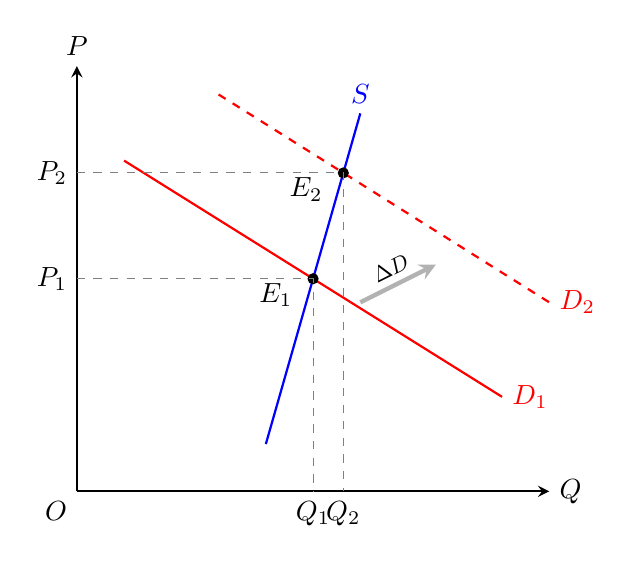
\begin{tikzpicture}[scale=1.2, >=stealth]
				% 坐标轴
				\draw[->, thick] (0,0) -- (5,0) node[right] {$Q$};
				\draw[->, thick] (0,0) -- (0,4.5) node[above] {$P$};
				\node[below left] at (0,0) {$O$};
				
				\draw[thick, blue] (2,0.5) -- (3,4) node[above] {$S$};
				
				% 初始需求曲线 D1
				\draw[thick, red] (0.5,3.5) -- (4.5,1) node[right] {$D_1$};
				
				% 新需求曲线 D2
				\draw[thick, red, dashed] (1.5,4.2) -- (5,2) node[right] {$D_2$};
				
				% 均衡点标注 
				\filldraw (2.5,2.25) circle (1.5pt) node[left, xshift=-4pt,yshift=-6pt] {$E_1$};
				\filldraw (2.82,3.37) circle (1.5pt) node[left, xshift=-4pt,yshift=-6pt] {$E_2$};
				
				% 价格与数量辅助线
				\draw[dashed, gray] (0,2.25) node[left, black] {$P_1$} -- (2.5,2.25) -- (2.5,0) node[below, black] {$Q_1$};
				\draw[dashed, gray] (0,3.37) node[left, black] {$P_2$} -- (2.82,3.37) -- (2.82,0) node[below, black] {$Q_2$};
				
				% 需求移动箭头
				\draw[->, ultra thick, gray!60] (3.0,2.0) -- (3.8,2.4) node[midway, sloped, above, scale=0.8, black] {$\Delta D$};
			\end{tikzpicture}
		\end{center}
		
		在短期内，由于生产商的产能和库存难以迅速调整，供给曲线通常表现得非常陡峭（即缺乏弹性）。当需求曲线从 $D_1$ 右移至 $D_2$ 时，在原均衡价格 $P_1$ 水平上会出现显著的短缺。
		
		这种短缺压力会促使未买到商品的消费者竞相出价，同时零售商也会随之提高售价。随着价格的攀升，一部分需求被抑制，最终在更高的价格水平 $P_2$ 上重新实现供需平衡。
		
			\item \textbf{运用供给曲线和需求曲线说明以下各事件会怎样影响黄油的价格以及黄油的销售量、购买量：}
			\begin{enumerate}[label=(\alph*), leftmargin=2em]
				\item \textbf{人造黄油价格上升；}
				\item \textbf{牛奶价格上升；}
				\item \textbf{平均收入水平下降。}
			\end{enumerate}
			
			\textbf{答：}
			分析这些事件对均衡价格（$P$）和均衡数量（$Q$）的影响，需识别受冲击的是需求侧还是供给侧。
			
				(a)人造黄油与黄油互为替代品。人造黄油价格上升，消费者会转而消费黄油，导致黄油需求增加，价格与销量同步上升。
				
				(b)牛奶是生产黄油的核心原材料。牛奶价格上涨抬高了生产成本，导致供给减少，表现为供给曲线向左上方移动。
				
				(c)黄油通常被视为正常商品。收入水平下降导致消费者购买力减弱，需求曲线向左下方移动。
			
			\item \textbf{如果玉米片的价格上升3\%致使其需求量下降6\%，那么玉米片的需求价格弹性是多少？}
			
			\textbf{答：}
			需求价格弹性的核心定义式如下：
				$$ E_d = \frac{\Delta Q / Q}{\Delta P /P} $$
			
			已知需求量变动 $-6\%$，价格变动 $3\%$。代入公式计算得：
				$$ E_d = \frac{-6\%}{3\%} = -2 $$
			由于 $|E_d| = 2 > 1$，说明玉米片的需求是富有弹性的。

			\item \textbf{试解释供给曲线的移动和沿着供给曲线的移动之间的区别。}
			
			\textbf{答：}
			这两者的根本区别在于引发变动的因素不同。
			
			沿着供给曲线的移动由商品自身价格变动引起。供给曲线整体位置保持不变，仅均衡点在原有供给曲线上上下滑动，仅改变供给数量，不改变供给整体水平。
			
			供给曲线的移动由生产成本、技术、相关品价格、预期等非价格因素变动引起。商品每一价格对应的供给数量整体发生改变，表现为整条供给曲线向左或向右平移，代表供给整体增加或减少。
			
			图形直观对比示意见下：
			
		\begin{center}
			\begin{tikzpicture}[scale=1.1, >=stealth]
				% --- 左图：供给曲线整体移动 ---
				\draw[->, thick] (0,0) -- (3.5,0) node[right] {$Q$};
				\draw[->, thick] (0,0) -- (0,3.5) node[above] {$P$};
				\draw[thick] (0.8,0.5) -- (3.2,3.2) node[above] {$S_1$};
				\draw[thick, dashed, blue] (0.2,0.5) -- (2.6,3.2) node[above] {$S_2$};
				
				\draw[->, blue, thick] (1.6,1.5) -- (1.2,1.5);
				\node[below] at (1.7, -0.4) {\textbf{(a) 曲线的移动 (线变动)}};
				
				% --- 右图：沿供给曲线点移动 ---
				\begin{scope}[xshift=5.5cm]
					\draw[->, thick] (0,0) -- (3.5,0) node[right] {$Q$};
					\draw[->, thick] (0,0) -- (0,3.5) node[above] {$P$};
					\draw[thick] (0.8,0.5) -- (3.2,3.2) node[above] {$S$};

					\coordinate (A) at (1.5,1.29);
					\coordinate (B) at (2.5,2.41);
					
					\fill (A) circle (1.5pt) node[below right] {$A$};
					\fill (B) circle (1.5pt) node[below right] {$B$};

					\draw[->, red, thick, bend right=25, shorten <=3pt, shorten >=3pt] (A) to (B);
					
					\node[below] at (1.7, -0.4) {\textbf{(b) 沿着曲线移动 (点变动)}};
				\end{scope}
			\end{tikzpicture}
		\end{center}
		\item \textbf{试解释为什么许多商品的长期需求弹性要大于短期需求弹性。}
		
		\textbf{答：}
		商品长期需求弹性大于短期需求弹性，核心源于消费者调整行为的时间差异。短期中，消费习惯与消费结构难以快速改变，替代品选择有限，面对价格波动，需求量仅能小幅调整，需求弹性较小。长期条件下，消费者可充分调整消费偏好、更换替代商品、优化消费方案，对价格变化做出充分反应。相同价格变动幅度下，长期需求量的调整幅度更大，因此长期需求弹性更高。
		
		\newpage
		\item \textbf{为什么长期需求弹性与短期需求弹性会有不同？考虑两种商品：纸巾和电视机。哪一种是耐用品？你觉得纸巾的短期需求价格弹性大，还是长期需求价格弹性大？为什么？电视机的需求价格弹性又是怎样的？}
		
		\textbf{答：}
		长期需求弹性与短期需求弹性存在差异，核心在于消费者调整行为所需的时间。电视机属于耐用品，纸巾为日常非耐用消耗品。二者的弹性特征对比如下表所示：
		
		\begin{center}
			\begin{tabularx}{\textwidth}{>{\centering\arraybackslash}X >{\centering\arraybackslash}X >{\centering\arraybackslash}X}
				\toprule
				\textbf{商品类别} & \textbf{短期需求价格弹性} & \textbf{长期需求价格弹性} \\
				\midrule
				纸巾（非耐用消耗品） & 较小 & 较大 \\
				电视机（耐用品） & 较大 & 较小 \\
				\bottomrule
			\end{tabularx}
		\end{center}

		\textbf{纸巾（非耐用消耗品）：长期需求价格弹性更大。}在短期内，人们的生活习惯和消费结构可能很难改变，对价格变化并没有太多反应；但是在长期中，人们会有充足的时间寻找替代品（如改用抹布)或者是改变自己的生活习惯，因此在这个过程中，需求量对于价格的反映就会变得更加灵敏一些。
		
		\textbf{电视机（耐用品）：短期需求价格弹性更大。}因为电视机购买往往具有一定延迟性。当电视机的价格短期上涨时，人们完全可以选择继续使用旧电视而不换新，其短期需求量会剧烈下降（弹性大）；但是在长期里，旧电视将最终报废，即便面临高昂的成本也必须要购买，所以从长期来看，它只有相对较小的需求量（弹性小）。
		
		\item \textbf{以下陈述是否正确？请解释。\\
			a. 需求的价格弹性等于需求曲线的斜率。\\
			b. 交叉价格弹性总是为正。\\
			c. 公寓的短期供给弹性要低于其长期供给弹性。}
		
		\textbf{答：}
		
		\textbf{a. 错误。}
		
		需求价格弹性核心公式如下：

			$$E_d = \frac{\Delta Q/Q}{\Delta P/P} = \frac{\Delta Q}{\Delta P} \cdot \frac{P}{Q}$$

		
		需求曲线斜率为 $\frac{\Delta P}{\Delta Q}$，二者并不等同。弹性除受斜率影响外，还受 $P/Q$ 比值影响。线性需求曲线上斜率恒定，但不同点位的 $P$ 和 $Q$ 不同，因此每一点需求价格弹性均不相等。
		
		\textbf{b. 错误。}
		
		交叉价格弹性核心公式如下：

			$$E_{XY} = \frac{\Delta Q_X/Q_X}{\Delta P_Y/P_Y}$$

		
		交叉价格弹性可正、可负，并非恒为正数。具体分类及其经济学含义如下表所示：
		
		\begin{center}
			\renewcommand{\tabularxcolumn}[1]{m{#1}}
			\begin{tabularx}{\textwidth}{>{\centering\arraybackslash}X >{\centering\arraybackslash}X >{\centering\arraybackslash}X}
				\toprule
				\textbf{商品关系} & \textbf{交叉价格弹性符号} & \textbf{特征描述} \\
				\midrule
				替代品 & 正数（$E_{XY} > 0$） & 一种商品价格上升，导致另一种商品需求量增加 \\
				互补品 & 负数（$E_{XY} < 0$） & 一种商品价格上升，导致另一种商品需求量减少 \\
				\bottomrule
			\end{tabularx}
		\end{center}

		\textbf{c. 正确。}
		
		公寓属于长期建设的不动产，短期房屋数量、楼栋规模难以调整，供给刚性强，短期供给弹性小；长期可通过新建、改造、盘活房源等方式调整供给数量，供给调整空间更大，因此长期供给弹性更高。
		
		\item \textbf{政府对牛肉、鸡肉实施低于市场出清水平的价格管制，分析其对市场及替代品的影响。}
		
		\textbf{答：}
		
		市场短缺状态的形成机制如下：
		\begin{tcolorbox}[colback=white, colframe=black!10, sharp corners, boxrule=0.5pt]
			$$\text{当 } P_{\text{限价}} < P_{\text{均衡}} \text{ 时，} Q_D > Q_S \implies \text{市场出现短缺}$$
		\end{tcolorbox}
		
		政府对牛肉、鸡肉实施低于市场出清水平的价格管制，属于最高限价政策。在管制低价下，生产者利润被压缩，供给量减少；消费者购买成本下降，需求量增加。由此形成 $Q_D > Q_S$ 的市场状态，出现商品短缺。短缺的规模由需求价格弹性与供给价格弹性共同决定：供需弹性越小，供需数量调整幅度越有限，短缺问题越突出。
		
		牛肉、鸡肉与猪肉互为替代品，前者因限价出现供给短缺时，消费者会转向消费猪肉，推动猪肉需求曲线右移，最终导致猪肉均衡价格上升。长期过低的行政限价，还会引发排队抢购、黑市交易、非价格配给等市场乱象，降低资源配置效率。
		
		\begin{center}
			\begin{tikzpicture}[scale=1.2, >=stealth]
				% --- 1. 定义坐标点  ---
				\coordinate (O) at (0,0);
				\coordinate (E) at (2.75, 2.75); 
				\coordinate (P_max_line) at (0, 1.75); 
				\coordinate (Qs_point) at (1.75, 1.75); 
				\coordinate (Qd_point) at (3.75, 1.75); 
				
				% --- 2. 绘制坐标轴 ---
				\draw[->, thick] (O) -- (6,0) node[right] {$Q$};
				\draw[->, thick] (O) -- (0,5) node[above] {$P$};
				\node[below left] at (O) {$O$};
				
				% --- 3. 绘制供给 S 与需求 D 曲线 ---
				\draw[thick] (0.8, 0.8) -- (4.5, 4.5) node[right] {$S$};
				\draw[thick] (0.8, 4.7) -- (4.8, 0.7) node[right] {$D$};
				
				% --- 4. 标注原均衡价格 P0 ---
				\draw[dashed, gray] (0, 2.75) node[left, black] {$P_0$} -- (E);
				\filldraw[black] (E) circle (1.5pt) node[above=2pt] {$E$};
				
				% --- 5. 绘制最高限价 (Price Ceiling) ---
				\draw[thick, blue] (0, 1.75) node[left] {$P_{\text{限价}}$} -- (5, 1.75);
				
				% 标注交点并投影到横轴
				\filldraw (Qs_point) circle (1.5pt);
				\filldraw (Qd_point) circle (1.5pt);
				
				\draw[dashed] (Qs_point) -- (1.75, 0) node[below] {$Q_s$};
				\draw[dashed] (Qd_point) -- (3.75, 0) node[below] {$Q_d$};
				
				% --- 6. 标注短缺区间 (Shortage) ---
				% 将箭头放在限价线上方一点，避免遮挡Q轴投影
				\draw[<->, red, thick] (1.75, 1.2) -- (3.75, 1.2) 
				node[midway, above, black, font=\small] {短缺};
				
			\end{tikzpicture}
		\end{center}
		\newpage
		\item \textbf{假设初始租房市场的市场出清租金为每月 700 美元。随着城市发展，租房需求增加，无管制的自由市场中新均衡租金上升至每月 900 美元。如果政府实施租金管制，设定最高租金限制为 700 美元。请分析：（1）租金变化与市场均衡情况；（2）租金管制是否对所有学生有利？}
		
		\textbf{答：}
		
		(1)租金变化与市场均衡分析
		
		初始租房市场自发均衡，市场出清租金为每月 700 美元。随城市发展，租房需求增加，需求曲线向右平移，在无管制的自由市场中，新均衡租金上升至每月 900 美元。
		
		政府实施租金管制，设定最高租金限制为 700 美元，该价格低于新市场均衡价格，属于限制性价格上限。短期住房供给弹性极低、供给数量近似固定；管制低价刺激租房需求进一步扩张，供给意愿小幅下降，市场出现供不应求与房源短缺。
		
		租金变动总结：自由市场下租金先由 700 美元上涨至 900 美元，管制政策将价格强行锁定在 700 美元，整体表现为先上升、后被管制压低。
		
		\begin{center}
			\begin{tikzpicture}[scale=0.8, >=stealth, thick, 
				dot/.style={circle, fill=black, inner sep=1pt}, every node/.style={scale=0.85}]
				
				% --- 1. 坐标轴 ---
				\draw[->] (0,0) coordinate(O) -- (7.5,0) node[right] {$Q$ \small (住房数量)};
				\draw[->] (0,0) -- (0,5.5) node[above] {$P$ \small (月租金/美元)};
				\node[below left] at (O) {$O$};
				
				% --- 2. 坐标点定义 ---
				\coordinate (E0) at (3, 2.5);     % 初始均衡点
				\coordinate (E1) at (3.5, 3.5);   % 新均衡点
				\coordinate (Qd_p) at (4.5, 2.5); % 限价下的新需求量点
				
				% --- 3. 绘制供需曲线 ---
				% 供给曲线 S
				\draw[black, ultra thick] (2, 0.5) -- (4.25, 5) node[right] {$S$};
				% 初始需求 D0
				\draw[black, thick] (1, 4.5) -- (5, 0.5) node[right] {$D_0$};
				% 新需求 D1
				\draw[blue, thick, dashed] (2.5, 4.5) -- (6.5, 0.5) node[right] {$D_1$};
				
				% --- 4. 需求曲线移动箭头 ---
				% 在上方空白处增加指示箭头，颜色与 D1 一致
				\draw[->, blue!80!black, thick] (1.9, 3.8) -- (3.0, 3.8) node[midway, above, font=\small] {};
				
				% --- 5. 价格上限线 (红色) ---
				\draw[red, ultra thick] (0, 2.5) -- (6.8, 2.5) 
				node[pos=0.1, above, text=red, font=\small\bfseries] {价格上限};
				
				% --- 6. 绘制垂直投影虚线 ---
				% 使用正交语法保证垂直
				\draw[dashed, gray] (E0) -- (E0 |- O) node[below, black] {$Q_0$};
				\draw[dashed, gray] (E1) -- (E1 |- O) node[below, black] {$Q_1$};
				\draw[dashed, gray] (Qd_p) -- (Qd_p |- O) node[below, black] {$Q_d$};
				
				% 仅保留 P1 的纵轴投影，移除 P0 投影
				\draw[dashed, gray] (E1) -- (O |- E1) node[left, black] {$P_1=900$};
				% 轴上的价格刻度（不需要虚线引导）
				\node[left] at (0, 2.5) {$P_0=700$};
				
				% --- 7. 标注交点 (调整位置防止遮挡) ---
				\node[dot] at (E0) {};
				\node[below left, xshift=-2pt] at (E0) {$E_0$}; % 移至左下方，避开 S 线
				
				\node[dot] at (E1) {};
				\node[right, xshift=3pt] at (E1) {$E_1$}; % 移至右侧，避开 D1 线
				
				\node[dot] at (Qd_p) {};
				
				% --- 8. 短缺标注 ---
				\draw[<->, red, very thick] ([yshift=-12pt]E0) -- ([yshift=-12pt]Qd_p) 
				node[midway, fill=white, inner sep=2pt, font=\small\bfseries] {短缺};
				
			\end{tikzpicture}
		\end{center}
		
		(2)租金管制是否对所有学生有利？
		
		否，政策带来福利分化，并非全体学生受益。对于已租房的在校学生，若无管制，房租将上涨至 900 美元/月；价格上限锁定租金为 700 美元，直接降低居住成本，福利改善。而对于尚未租房的潜在租客，短期住房供给刚性、房源总量有限。管制低价催生超额需求，房源竞争加剧，大量学生难以租到住房；同时易出现居住条件下降、隐性收费等问题，该群体利益受损。
		
		\item \textbf{某大学官员宣称，学费上涨并未减少申请入学的人数，反而由于该校声誉和教育质量的提升，申请人数显著增加。他据此认为该校的入学需求是完全无弹性的。请评述该官员的观点。}
		
		\textbf{答：}
		该大学官员的观点是错的。其核心在于混淆了“需求量的变动”与“需求的变动”，未能遵循经济学分析中“其他条件不变”的准则。
		
		该官员认为学费上涨没有减少申请人数，证明需求完全无弹性（即需求曲线是垂直的）。然而，经济学原理告诉我们，在其他条件不变的前提下，学费作为价格，其上涨必然导致需求量下降。
		
		现实中申请人数不降反升，并不是因为需求没有弹性，而是因为需求曲线发生了整体右移。该官员提到的“声誉提升”和“质量改善”，以及居民收入增加等因素，都是影响需求的非价格变量。这些因素的正面冲击足以抵消学费上涨带来的需求量缩减，导致最终观察到的均衡数量增加。
		
		市场变动示意图如下：
		\begin{center}
			\begin{tikzpicture}[scale=0.8, >=stealth, thick, 
				dot/.style={circle, fill=black, inner sep=1pt}, every node/.style={scale=0.85}]
				
				% --- 1. 坐标轴 ---
				\draw[->] (0,0) coordinate(O) -- (7,0) node[right] {$Q$ \small (申请人数)};
				\draw[->] (0,0) -- (0,5.5) node[above] {$P$ \small (学费)};
				\node[below left] at (O) {$O$};
				
				% --- 2. 坐标点 (根据直线方程求解) ---
				\coordinate (E0) at (3, 3);
				\coordinate (Qa) at (1.933, 3.8); 
				\coordinate (E1) at (3.433, 3.8); 
				
				% --- 3. 需求曲线 ---
				% 原需求 D0 (黑色)
				\draw[black, thick] (1, 4.5) -- (5, 1.5) node[below right] {$D_0$};
				% 新需求 D1 (蓝色虚线，代表右移)
				\draw[blue, thick, dashed] (2.5, 4.5) -- (6.5, 1.5) node[below right] {$D_1$};
				% 官员脑补的垂直需求曲线 (灰色点线)
				\draw[gray, dotted, ultra thick] (3, 0.5) -- (3, 5) node[above, font=\small, text=gray] {官员假设的 $D$};
				
				% --- 4. 均衡点与投影 ---
				% 初始均衡 E0
				\draw[dashed, gray] (E0) -- (0, 3) node[left, black] {$P_0$};
				\draw[dashed, gray] (E0) -- (3, 0) node[below, black] {$Q_0$};
				\node[dot] at (E0) {};
				\node[below left] at (E0) {$E_0$};
				
				% 涨价后的横向价格线 P1，贯穿 Qa 和 E1
				\draw[dashed, gray] (0, 3.8) node[left, black] {$P_1$} -- (E1);
				
				% 沿 D0 移动的 Qa 点 (价格效应终点)
				\draw[dashed, gray] (Qa) -- (Qa |- O) node[below, black] {$Q'$};
				\node[dot] at (Qa) {};
				
				% 最终新均衡 E1
				\draw[dashed, gray] (E1) -- (E1 |- O) node[below, black] {$Q_1$};
				\node[dot] at (E1) {};
				\node[above right] at (E1) {$E_1$};
				
				% --- 5. 动态标注 ---
				% 需求移动箭头
				\draw[->, blue!80!black, ultra thick] (3.8, 2.4) -- (5.2, 2.4) ;
				
				% 价格上涨引起的点动箭头
				\draw[->, red, very thick, bend right=15, shorten <=3pt, shorten >=3pt] (E0) to (Qa);
				
			\end{tikzpicture}
		\end{center}
		
		结论：该官员将“需求的变动”（曲线右移）错误地解读为“需求完全无弹性”。如果该校保持学费不变，申请人数本应增加更多（增加到 $D_1$ 在 $P_0$ 对应的水平）。因此，不能依据学费和人数同步增长的事实来断定需求缺乏弹性。

		\item \textbf{假设某种商品的需求曲线为 $Q=10-2P+P_S$，其中，$P$ 是该商品的价格，$P_S$ 是某种替代品的价格。已知该替代品的价格是 $2.00$ 美元。a. 如果 $P=1.00$ 美元，需求的价格弹性等于多少？交叉价格弹性又等于多少？b. 如果该商品的价格 $P$ 上升至 $2.00$ 美元，那么现在需求的价格弹性又是多少？交叉价格弹性呢？}
		
		\textbf{答：}
		将已知替代品价格 $P_S = 2.00$ 代入需求函数，可得化简后的商品需求方程：
		$$Q = 12 - 2P$$
		根据点弹性定义，建立需求价格弹性与交叉价格弹性的核心计算公式：

			$$
			\begin{aligned}
				E_d &= \frac{\partial Q}{\partial P} \cdot \frac{P}{Q}\\
				E_{xy} &= \frac{\partial Q}{\partial P_S} \cdot \frac{P_S}{Q}
			\end{aligned}
			$$

		
		a.当商品价格 $P = 1.00$ 时，对应的市场需求量为 $Q = 10$。代入核心公式计算可得：
		$$
		\begin{aligned}
			E_d &= -2 \times \frac{1.00}{10} = -0.2 \\
			E_{xy} &= \frac{2.00}{10} = 0.2
		\end{aligned}
		$$
		此时 $|E_d| < 1$，表明该价格水平下需求缺乏弹性；$E_{xy} > 0$ 则验证了两种商品互为替代品的经济关系。
		
		b.当商品价格上升至 $P = 2.00$ 时，需求量缩减为 $Q = 8$。重新测算两类弹性：
		$$
		\begin{aligned}
			E_d &= -2 \times \frac{2.00}{8} = -0.5 \\
			E_{xy} &= \frac{2.00}{8} = 0.25
		\end{aligned}
		$$
		计算结果表明，随着价格沿线性需求曲线向上攀升，需求价格弹性的绝对值逐渐增大，消费者对价格变动的敏感度提升。

		\item \textbf{已知铜市场的初始需求曲线为 $Q_d = 27 - 3P$，初始供给曲线为 $Q_s = -9 + 9P$。若生产成本下降导致供给曲线向右移动 40\%，请推导新的供给曲线，计算新的市场均衡，并结合图形分析市场的具体变动。}
		
		\textbf{答：}
		在原有市场结构下，若生产成本发生下降，生产者在任何给定的价格水平下都有能力且愿意提供更多的产品。根据题意，供给曲线整体向右移动 40\%，等价于新供给量等于原供给量的 1.4 倍。由此可推导出新的供给函数方程：
			$$Q'_s = 1.4(-9 + 9P) = -12.6 + 12.6P$$
		
		市场出清原则要求新的总供给量必须等于总需求量。令原需求曲线 $Q_d$ 与新供给曲线 $Q'_s$ 相等，构建均衡等式进行求解：
		$$
		\begin{aligned}
			Q_d &= Q'_s \\
			P &\approx 2.54 \text{ 美元/磅}
		\end{aligned}
		$$
		将计算得到的新均衡价格代回原需求方程，可求得此时的新均衡交易量为 $Q \approx 27 - 3(2.54) = 19.38 \text{ 百万公吨/年}$。

		\begin{center}
			\begin{tikzpicture}[x=0.1875cm, y=0.9cm, >=stealth, every node/.style={scale=0.85}]
				% 坐标轴
				\draw[->, thick] (0,0) -- (28,0) node[right] {$Q \text{ (百万公吨/年)}$};
				\draw[->, thick] (0,0) -- (0,5.5) node[above] {$P \text{ (美元/磅)}$};
				
				% 原需求曲线 D: P = 9 - Q/3 
				\draw[thick, name path=demand] (10, 5.67) -- (26, 0.33) node[below right] {$D$};
				
				% 原供给曲线 S: P = 1 + Q/9 
				\draw[thick, name path=supply0] (4.5, 1.5) -- (26, 3.89) node[above right] {$S$};
				
				% 新供给曲线 S': P = 1 + Q/12.6 
				\draw[thick, blue, dashed, name path=supply1] (6.3, 1.5) -- (26, 3.06) node[right] {$S'$};
				
				% 初始均衡点 E
				\coordinate (E0) at (18, 3);
				\fill (E0) circle (2pt) node[above=4pt, fill=white, inner sep=1pt] {$E$};
				\draw[dashed] (E0) -- (E0 |- 0,0) node[below, fill=white, inner sep=1pt] {$18$};
				\draw[dashed] (E0) -- (0,0 |- E0) node[left] {$3.00$};
				
				% 新均衡点 E'
				\coordinate (E1) at (19.38, 2.54);
				\fill (E1) circle (2pt) node[below left=2pt, fill=white, inner sep=1pt] {$E'$};
				\draw[dashed] (E1) -- (E1 |- 0,0) node[below, fill=white, inner sep=1pt] {$19.38$};
				\draw[dashed] (E1) -- (0,0 |- E1) node[left] {$2.54$};
				
				\coordinate (A) at (9, 2);
				\coordinate (B) at (12, 2);
				\draw[->, thick, blue, shorten <=3pt, shorten >=3pt] (A) -- (B);
			\end{tikzpicture}
		\end{center}

		\item \textbf{假设天然气的需求是完全无弹性的，那么对天然气的价格控制可能会导致什么样的后果？}
		
		\textbf{答：}
		如果天然气的需求完全没有弹性，无论价格怎么变，消费者购买的数量固定。在坐标轴里，需求曲线就是一条垂直的直线。
		
		这时，如果政府干预价格，市场失衡的程度主要取决于供给方的反应。限价或保价政策，会引向截然不同的局面。供应越灵活，市场缺口（无论是短缺还是过剩）就拉得越大。以下是两种政策下的市场变动分析：
		\begin{center}
			\begin{tikzpicture}[scale=1.1, >=stealth]
				% ---------- 左图：最低限价（供给过剩） ----------
				\begin{scope}[shift={(0,0)}]
					% 坐标轴
					\draw[->, thick] (0,0) -- (4.5,0) node[right] {$Q$};
					\draw[->, thick] (0,0) -- (0,4.5) node[above] {$P$};
					
					% 完全无弹性需求曲线 D（垂直，基准线黑）
					\draw[thick, name path=demand1] (2,0) -- (2,4.3) node[above] {$D$};
					
					% 供给曲线 S（基准线黑）
					\draw[thick, name path=supply1] (0.5,0.5) -- (3.5,3.5) node[above right] {$S$};
					
					% 均衡点 E
					\coordinate (E1) at (2,2);
					\fill (E1) circle (1.5pt) node[above left] {$E$};
					\draw[dashed] (E1) -- (E1 |- 0,0) node[below] {$Q^*$};
					\draw[dashed] (E1) -- (0,0 |- E1) node[left] {$P^*$};
					
					% 最低限价 Pmin (政策限制线，红粗)
					\draw[very thick, red] (0,3) node[left] {$P_{\min}$} -- (4,3);
					
					% 供给点与需求点投影
					\coordinate (S1) at (3,3);
					\coordinate (D1) at (2,3);
					\fill (S1) circle (1.5pt);
					\fill (D1) circle (1.5pt);
					\draw[dashed] (S1) -- (S1 |- 0,0) node[below] {$Q_s$};
					
					% 标识失衡区间
					\draw[<->, thick, shorten <=2pt, shorten >=2pt] (2, 0.5) -- (3, 0.5) node[midway, below] {\small 过剩};
				\end{scope}
				
				% ---------- 右图：最高限价（供给短缺） ----------
				\begin{scope}[shift={(6,0)}]
					% 坐标轴
					\draw[->, thick] (0,0) -- (4.5,0) node[right] {$Q$};
					\draw[->, thick] (0,0) -- (0,4.5) node[above] {$P$};
					
					% 完全无弹性需求曲线 D（垂直，基准线黑）
					\draw[thick, name path=demand2] (2,0) -- (2,4.3) node[above] {$D$};
					
					% 供给曲线 S（基准线黑）
					\draw[thick, name path=supply2] (0.5,0.5) -- (3.5,3.5) node[above right] {$S$};
					
					% 均衡点 E
					\coordinate (E2) at (2,2);
					\fill (E2) circle (1.5pt) node[above left] {$E$};
					\draw[dashed] (E2) -- (E2 |- 0,0) node[below] {$Q^*$};
					\draw[dashed] (E2) -- (0,0 |- E2) node[left] {$P^*$};
					
					% 最高限价 P_max (政策限制线，红粗)
					\draw[very thick, red] (0,1) node[left] {$P_{\max}$} -- (4,1);
					
					% 供给点与需求点投影
					\coordinate (S2) at (1,1);
					\coordinate (D2) at (2,1);
					\fill (S2) circle (1.5pt);
					\fill (D2) circle (1.5pt);
					\draw[dashed] (S2) -- (S2 |- 0,0) node[below] {$Q_s$};
					
					% 标识失衡区间
					\draw[<->, thick, shorten <=2pt, shorten >=2pt] (1, 0.5) -- (2, 0.5) node[midway, below] {\small 短缺};
				\end{scope}
			\end{tikzpicture}
		\end{center}
	\end{enumerate}
	\newpage
	\section{练习题}
		\begin{enumerate}[label=\textbf{\arabic*.}, leftmargin=*]
			\item \textbf{假设某种商品的需求曲线是 $Q=300-2P+4I$，其中 $I$ 是以千美元计量的收入。供给曲线是 $Q=3P-50$。请分别求解当 $I=25$ 和 $I=50$ 时的市场出清价格与数量，并画图说明。}
			
			\textbf{答：}
			当 $I=25$ 时，代入需求函数可得当期需求曲线为 $Q_d = 400 - 2P$。根据市场出清条件 $Q_d = Q_s$，直接列式：
			$$ 400 - 2P = 3P - 50 \implies P = 90,\ Q = 220 $$
			当 $I=50$ 时，需求曲线变动为 $Q_d = 500 - 2P$。同理：
			$$ 500 - 2P = 3P - 50 \implies P = 110,\ Q = 280 $$
			由此可见，收入增加使得需求曲线整体右移，带动市场均衡价格与数量双双上升。其市场供需变动图形如下：
			\begin{center}
				\begin{tikzpicture}[x=0.0225cm, y=0.0375cm, >=stealth, every node/.style={scale=0.8}]
					% 坐标轴
					\draw[->, thick] (0,0) -- (350,0) node[right] {$Q$};
					\draw[->, thick] (0,0) -- (0,150) node[above] {$P$};
					
					% 供给与需求曲线
					\draw[thick, name path=S] (50, 33.33) -- (320, 123.33) node[above right] {$S$};
					\draw[thick, name path=D1] (100, 150) -- (300, 50) node[below right] {$D_1 (I=25)$};
					\draw[thick, blue, dashed, name path=D2] (160, 170) -- (320, 90) node[right] {$D_2 (I=50)$};
					
					% 均衡点 E1
					\coordinate (E1) at (220, 90);
					\fill (E1) circle (1.5pt) node[below left=2pt, fill=white, inner sep=1pt] {$E_1$};
					\draw[dashed] (E1) -- (E1 |- 0,0) node[below] {$220$};
					\draw[dashed] (E1) -- (0,0 |- E1) node[left] {$90$};
					
					% 均衡点 E2
					\coordinate (E2) at (280, 110);
					\fill (E2) circle (1.5pt) node[above right=2pt, fill=white, inner sep=1pt] {$E_2$};
					\draw[dashed] (E2) -- (E2 |- 0,0) node[below] {$280$};
					\draw[dashed] (E2) -- (0,0 |- E2) node[left] {$110$};
					
					% 需求右移指示箭头
					\draw[->, thick, blue, shorten <=4pt, shorten >=4pt] (160, 120) -- (250, 120) node[midway, below, fill=white, inner sep=1pt] {\small \text{需求增加}};
				\end{tikzpicture}
			\end{center}
			
			
			\item \textbf{考虑一个竞争性市场，在不同价格下，需求量和供给量如下表所示。请计算价格在 80 美元至 100 美元区间的需求/供给价格弹性，指出均衡状态，并分析 80 美元最高限价的政策影响。}
			\begin{center}
				\begin{tabularx}{\textwidth}{>{\centering\arraybackslash}X >{\centering\arraybackslash}X >{\centering\arraybackslash}X}
					\toprule
					\textbf{价格（美元）} & \textbf{需求量（百万）} & \textbf{供给量（百万）} \\
					\midrule
					60 & 22 & 14 \\
					80 & 20 & 16 \\
					100 & 18 & 18 \\
					120 & 16 & 20 \\
					\bottomrule
				\end{tabularx}
			\end{center}
			
			\textbf{答：}
			首先，计算需求与供给价格弹性。在 80 至 100 美元区间，需求曲线斜率为$-0.1$，供给曲线斜率为 $0.1$。用点弹性核心公式进行计算：
				$$ E = \frac{\Delta Q}{\Delta P} \cdot \frac{P}{Q} $$
			将对应数据代入公式，直接求解得出：
			$$
			\begin{aligned}
				\text{当 } P=80 \text{ 时：} & E_d = -0.1 \times \frac{80}{20} = -0.4, \quad E_s = 0.1 \times \frac{80}{16} = 0.5 \\
				\text{当 } P=100 \text{ 时：} & E_d = -0.1 \times \frac{100}{18} \approx -0.56, \quad E_s = 0.1 \times \frac{100}{18} \approx 0.56
			\end{aligned}
			$$
			
			由表格数据直观可知，当价格 $P=100$ 美元时，市场需求量等于供给量，即均衡价格 $P^* = 100$，均衡数量 $Q^* = 18$。
			
			若政府设定80美元的最高限价，该价格低于均衡价格，属于有效价格干预。此时市场需求量上升至20，而供给量降低至16，直接列式计算短缺缺口：
			$$ \text{短缺量} = Q_d - Q_s = 20 - 16 = 4 $$
			\begin{center}
				\begin{tikzpicture}[x=0.3cm, y=0.0375cm, >=stealth, every node/.style={scale=0.8}]
					% 坐标轴
					\draw[->, thick] (0,0) -- (26,0) node[right] {$Q \text{ (百万)}$};
					\draw[->, thick] (0,0) -- (0,150) node[above] {$P \text{ (美元)}$};
					
					% 需求与供给曲线
					\draw[thick, name path=demand] (14, 140) -- (24, 40) node[below right] {$D$};
					\draw[thick, name path=supply] (12, 40) -- (22, 140) node[above right] {$S$};
					
					% 均衡点 E
					\coordinate (E) at (18, 100);
					\fill (E) circle (1.5pt) node[above=4pt] {$E$};
					\draw[dashed] (E) -- (E |- 0,0) node[below] {$18$};
					\draw[dashed] (E) -- (0,0 |- E) node[left] {$100$};
					
					% 最高限价 (政策线，红粗)
					\draw[very thick, red] (0, 80) node[left] {$80$} -- (25, 80) node[right] {$P_{\max}$};
					
					% 短缺投影与标识
					\coordinate (Qs) at (16, 80);
					\coordinate (Qd) at (20, 80);
					\fill (Qs) circle (1.5pt);
					\fill (Qd) circle (1.5pt);
					\draw[dashed] (Qs) -- (Qs |- 0,0) node[below] {$16$};
					\draw[dashed] (Qd) -- (Qd |- 0,0) node[below] {$20$};
					
					% 调整短缺标识的比例
					\draw[<->, thick, shorten <=2pt, shorten >=2pt] (16, 20) -- (20, 20) node[midway, below, fill=white, inner sep=1pt] {\small $\text{短缺}$};
				\end{tikzpicture}
			\end{center}
			
			\item \textbf{在 1998 年，美国对小麦的需求函数为 $Q_d = 3244 - 283P$，本国供给函数为 $Q_s = 1944 + 207P$。假设巴西和印度尼西亚开放市场后，美国小麦的需求增加了 200 百万蒲式耳。求新的完全竞争均衡价格与产量。}
			
			\textbf{答：}
			国际市场的开放导致美国小麦需求增加。这表现为在任何给定的价格水平下，需求量均增加 200 百万蒲式耳。因此，新的市场需求函数方程变为：
			$$Q'_d = (3244 - 283P) + 200 = 3444 - 283P$$
			
			在供给曲线 $Q_s = 1944 + 207P$ 保持不变的情况下，令新需求等于供给 $Q'_d = Q_s$，直接列式计算新的市场出清状态：
			$$3444 - 283P = 1944 + 207P \implies P \approx 3.06 \text{ 美元},\ Q \approx 2577 \text{ 百万蒲式耳}$$
			
			外部市场开放带来的需求扩张直接拉高了小麦的市场价格，并同时推高了总产出规模。

			\item \textbf{一种植物纤维在竞争性的世界市场上进行贸易，世界市场价格为9美元/磅。在该价格下，美国可以得到无限多的进口商品。在不同的价格水平下，美国国内市场的供给和需求如下表所示：}
			
			\begin{center}
				\begin{tabularx}{\textwidth}{>{\centering\arraybackslash}X >{\centering\arraybackslash}X >{\centering\arraybackslash}X}
					\toprule
					\textbf{价格} & \textbf{美国的供给（百万磅）} & \textbf{美国的需求（百万磅）} \\
					\midrule
					3  & 2  & 34 \\
					6  & 4  & 28 \\
					9  & 6  & 22 \\
					12 & 8  & 16 \\
					15 & 10 & 10 \\
					18 & 12 & 4  \\
					\bottomrule
				\end{tabularx}
			\end{center}
			
			\textbf{a. 求出需求方程和供给方程。\\
				b. 在价格等于9美元处，需求的价格弹性是多少？在价格等于12美元处呢？\\
				c. 在价格等于9美元处，供给的价格弹性是多少？在价格等于12美元处呢？\\
				d. 在自由市场上，植物纤维在美国的价格是多少？此时的进口数量是多少？}
			
			\textbf{答：}
			
			(a) 联立表格数据得：
				$$Q_d = 40 - 2P,\quad Q_s = \frac{2}{3}P$$
			(b) 需求价格弹性：
				$$E_d = \frac{dQ_d}{dP} \cdot \frac{P}{Q_d}$$
				
				$P=9$ 时：$Q_d=22 \implies E_d = -0.82$\\
				$P=12$ 时：$Q_d=16 \implies E_d = -1.5$\\
			(c) 供给价格弹性：
				$$E_s = \frac{dQ_s}{dP} \cdot \frac{P}{Q_s}$$

				$P=9$ 时：$Q_s=6 \implies E_s = 1$\\
				$P=12$ 时：$Q_s=8 \implies E_s = 1$

			(d) 自由市场价格与进口量
			
			1. 封闭国内均衡：令 $Q_d = Q_s$，解得国内自给自足均衡价 $P=15$ 美元。
			
			2. 开放自由市场：世界价格 $9$ 美元更低，美国国内价格等于世界价格 $P=9$ 美元。
			
			3. 进口量计算：
				$$\text{进口} = Q_d - Q_s = 22 - 6 = 16 \text{（百万磅）}$$
				
			\item \textbf{对美国农产品的需求很多是来自其他国家。如在1998年，小麦的总需求是 $Q=3244-283P$，其中美国国内的需求为 $Q_D=1700-107P$，国内的供给是 $Q_S=1944+207P$。假设小麦的出口需求下降了40\%。\\
				a. 美国农民注意到出口需求下降了，这对于美国小麦的自由市场价格会产生什么影响？农民有理由担心吗？\\
				b. 现在假设美国政府想要购买足够的小麦使得价格上升至3.50美元/蒲式耳，如果没有出口需求，政府需要购买多少小麦？政府的购买行为需要支付多少货币？}
			
			\textbf{答：}
			
			(a) 出口需求下降对自由市场价格的影响
			
			计算原出口需求和下降后的新总需求：
				$$Q_{ex0} = Q - Q_D = 1544 - 176P$$
				$$Q_{ex1} = 0.6 \cdot Q_{ex0} = 926.4 - 105.6P$$
				$$Q' = Q_D + Q_{ex1} = 2626.4 - 212.6P$$
			
			计算原均衡价格（令 $Q = Q_S$）与新均衡价格（令 $Q' = Q_S$）：
				$$3244 - 283P_0 = 1944 + 207P_0 \implies P_0 \approx 2.65$$
				$$2626.4 - 212.6P_1 = 1944 + 207P_1 \implies P_1 \approx 1.63$$
			
			自由市场价格从约 2.65 美元/蒲式耳下降至约 1.63 美元/蒲式耳。由于价格大幅下跌会导致农民收入显著减少，因此农民有理由担心。
			
			(b) 政府干预下的购买量与支出（无出口需求，目标价格 $P=3.50$）
			
			当价格为 $P=3.50$ 时，国内的供给量与需求量：
				$$Q_D = 1700 - 107(3.5) = 1325.5$$
				$$Q_S = 1944 + 207(3.5) = 2668.5$$
			
			政府为了维持该价格需要购买过剩的供给，其购买量与总支出为：
				$$Q_{gov} = Q_S - Q_D = 2668.5 - 1325.5 = 1343$$
				$$\text{支出} = 1343 \times 3.5 = 4700.5$$

			结论：政府需要购买 1343 单位小麦，总购买行为需要支付 4700.5 美元。
			
			\item \textbf{纽约市住房总需求为 $Q_D = 160 - 8P$（单位：万间套房），住房供给为 $Q_S = 70 + 7P$（$P$：月租金，单位：百美元）。已知每套住房对应一个三口之家。\\
				a. 求自由市场均衡价格，并计算设定 300 美元租金上限对住房短缺及人口的影响。\\
				b. 若政府设定租金为 900 美元，且由此增加的住房供给中有 50\% 来自新建筑，求需建造的新住房数量。}
			
			\textbf{答：}
			
			(a) 自由市场均衡与租金上限影响：
			$$160 - 8P = 70 + 7P \implies P = 6,\ Q = 112$$
			自由市场月租金为 600 美元，住房数量为 112 万间。
			
			租金上限 $P=3$：$Q_D=136,\ Q_S=91 \implies \text{短缺} = 45$ 万间。
			
			$45 \times 3 = 135$ 万人。因住房短缺，纽约市人口将减少 135 万人。
			
			(b) 900 美元租金下的住房建设需求（$P=9$）：
			$$Q_S = 133,\quad \Delta Q_S = 133 - 112 = 21$$
			
			新建比例 50\%：$Q_{\text{新建}} = 21 \times 50\% = 10.5$ 万间。
			
			\begin{center}
				\begin{minipage}[t]{0.48\textwidth}
					\centering
					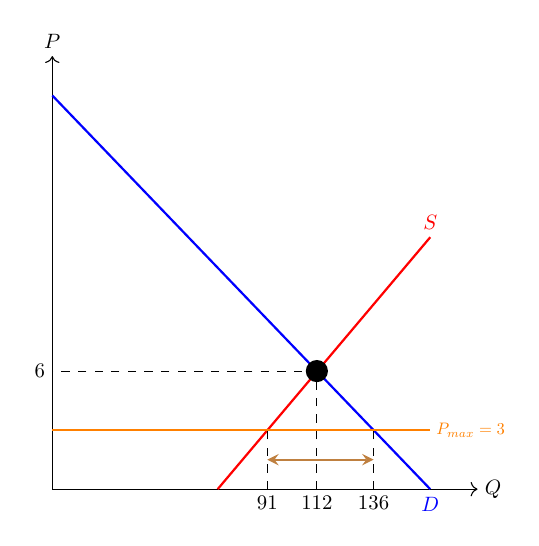
\begin{tikzpicture}[x=0.3cm, y=0.25cm, every node/.style={scale=0.75}]
						% 坐标轴
						\draw[->] (0,0) -- (18,0) node[right] {$Q$};
						\draw[->] (0,0) -- (0,22) node[above] {$P$};
						% 需求曲线 P = 20 - 0.125Q (Q=160, P=20)
						\draw[thick, blue] (0,20) -- (16,0) node[below] {$D$};
						% 供给曲线 P = (Q-70)/7 (Q=160, P~12.8)
						\draw[thick, red] (7,0) -- (16,12.8) node[above] {$S$};
						% 均衡点 E(112, 6)
						\draw[dashed] (11.2,0) node[below] {112} -- (11.2,6) -- (0,6) node[left] {6};
						\fill (11.2,6) circle (4pt);
						% 租金上限 P=3
						\draw[thick, orange] (0,3) -- (16,3) node[right, scale=0.8] {$P_{max}=3$};
						\draw[dashed] (9.1,0) node[below] {91} -- (9.1,3);
						\draw[dashed] (13.6,0) node[below] {136} -- (13.6,3);
						% 短缺箭头
						\draw[<->, >=stealth, thick, brown] (9.1,1.5) -- (13.6,1.5);
					\end{tikzpicture}
					
					\vspace{0.5em}
					{\small (a) 租金上限与短缺}
				\end{minipage}%
				\hfill
				\begin{minipage}[t]{0.48\textwidth}
					\centering
					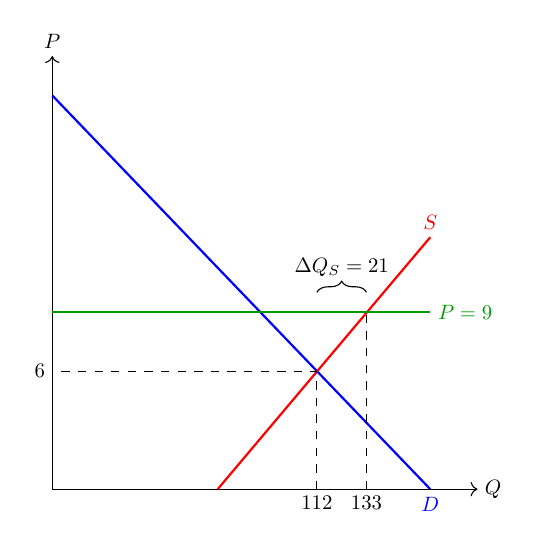
\begin{tikzpicture}[x=0.3cm, y=0.25cm, every node/.style={scale=0.75}]
						% 坐标轴
						\draw[->] (0,0) -- (18,0) node[right] {$Q$};
						\draw[->] (0,0) -- (0,22) node[above] {$P$};
						% 需求与供给
						\draw[thick, blue] (0,20) -- (16,0) node[below] {$D$};
						\draw[thick, red] (7,0) -- (16,12.8) node[above] {$S$};
						% 原均衡点参考
						\draw[dashed, black] (11.2,0) node[below] {112} -- (11.2,6) -- (0,6) node[left] {6};
						% 价格设定 P=9
						\draw[thick, green!60!black] (0,9) -- (16,9) node[right] {$P=9$};
						\draw[dashed] (13.3,0) node[below] {133} -- (13.3,9);
						% 供给增量括号
						\draw[decorate, decoration={brace, amplitude=4pt}] (11.2,10) -- (13.3,10) node[midway, above=4pt] {$\Delta Q_S=21$};
					\end{tikzpicture}
					
					\vspace{0.5em}
					{\small (b) 租金上升与供给增加}
				\end{minipage}
			\end{center}
			
			\newpage
			\item \textbf{2010年，美国人总共消费了3150亿支香烟，合157.5亿包。香烟的每包零售价（含税）大约平均为5美元。统计研究表明，需求的价格弹性是$-0.4$，供给的价格弹性是$0.5$。}
			
			\textbf{(a)根据这些信息，请推导香烟市场的线性需求曲线和线性供给曲线。}
			
			\textbf{答：}
			首先明确线性供需曲线的通用形式：
				$$ \text{需求曲线：} Q_d = a - bP $$
				$$ \text{供给曲线：} Q_s = c + dP $$
			
			根据已知均衡点 $Q^* = 157.5$，$P^* = 5$，推导过程如下：
			
			1. 求解需求曲线 \\
			利用点弹性公式 $$E_d = \frac{dQ_d}{dP} \cdot \frac{P^*}{Q^*}$$
			代入数据：
			$$ -0.4 = -b \cdot \frac{5}{157.5} \implies b = 12.6 $$
			将均衡点代入需求方程求解截距 $a = 220.5$\\
			得线性需求曲线为：$Q_d = 220.5 - 12.6P$。
			
			2. 求解供给曲线 \\
			利用点弹性公式 $$E_s = \frac{dQ_s}{dP} \cdot \frac{P^*}{Q^*}$$
			代入数据：
			$$ 0.5 = d \cdot \frac{5}{157.5} \implies d = 15.75 $$
			将均衡点代入供给方程求解截距 $c = 78.75$\\
			得线性供给曲线为：$\boldsymbol{Q_s = 78.75 + 15.75P}$。
			
			 \textbf{(b)1998年，美国人共消费了235亿包香烟，每包零售价为2美元。1998—2010年，香烟消费下降的部分原因是人们更多地认识到吸烟对健康的危害，部分原因是价格的上升。假设消费下降的所有原因都是价格上升，你可以推断出需求的价格弹性具有什么特征吗？}
			
			若假定消费下降完全由价格上涨导致，则意味着需求曲线未发生位移，观测到的变动完全是沿着同一条需求曲线的点移动。基于此假设，我们计算需求弧弹性：

				$$ E_d = \frac{\Delta Q}{\Delta P} \cdot \frac{(P_1 + P_2)/2}{(Q_1 + Q_2)/2} $$
			
			已知 1998 年数据为 $(P_1, Q_1) = (2, 235)$，2010 年数据为 $(P_2, Q_2) = (5, 157.5)$：
			$$ \Delta Q = 157.5 - 235 = -77.5, \quad \Delta P = 5 - 2 = 3 $$
			代入弧弹性公式：
			$$ \begin{aligned}
				E_d &= \frac{-77.5}{3} \cdot \frac{(2 + 5)/2}{(235 + 157.5)/2} \\
				& \approx -0.46
			\end{aligned} $$
			
			根据计算结果，可以推断该需求具有以下特征：
			\begin{enumerate}
				\item \textbf{需求缺乏弹性}：由于 $|E_d| \approx 0.46 < 1$，香烟需求表现为缺乏弹性。这意味着价格大幅上升仅引起消费量较小幅度的下降。
				\item \textbf{刚需属性}：长期来看，即便将所有消费降幅归结为价格因素，弹性系数依旧偏低。这印证了香烟作为成瘾性商品，消费者对其价格敏感度较低。
				\item \textbf{长期与短期的差异}：对比 2010 年的短期点弹性（$-0.4$）与该长期弧弹性（约 $-0.46$），可以看出随着时间推移，消费者通过调整习惯等方式，对价格的反应会比短期稍微灵敏一些。
			\end{enumerate}

			\item \textbf{在例2.8中，通过第2.6节中推导出来的线性供给曲线和线性需求曲线，我们研究了铜的需求量下降20\%对铜价的影响。假设铜的长期价格弹性是$-0.75$，而非$-0.5$。例题已知初始条件：铜的供给曲线 $Q_s = -9 + 9P$；初始均衡价格 $P^* = 3$ 美元/磅，均衡数量 $Q^* = 18$ 百万公吨/年。}
			
			\begin{enumerate}[label=\textbf{\alph*.}, leftmargin=2em]
				\item \textbf{如前假定，均衡价格和数量为 $P^* = 3$ 美元/磅，$Q^* = 18$ 百万公吨/年，试推导出与更小的需求弹性相一致的线性需求曲线。}
				\item \textbf{运用这一需求曲线，重新计算铜的需求下降55\%对铜价的影响。}
			\end{enumerate}
			
			\textbf{答：}
			
			\textbf{a.} 首先推导新的线性需求曲线。设线性需求曲线为：
				$$ Q_d = a - bP $$
			
			根据需求价格点弹性的定义公式 
			$$E_d = \frac{dQ_d}{dP} \cdot \frac{P}{Q}$$
			将已知的均衡点 $(P^*, Q^*) = (3, 18)$ 以及新的需求价格弹性 $E_d = -0.75$ 代入公式计算：
			$$ -0.75 = -b \cdot \frac{3}{18} $$
			解得 $b = 4.5$。
			
			接着，将市场均衡点和求得的斜率系数代入需求曲线方程，得解截距 $a = 31.5 $

			因此，与更小需求弹性相一致的新线性需求曲线方程为：
			$$ Q_d = 31.5 - 4.5P $$
			
			\vspace{1em}
			
			\textbf{b.} 接下来重新计算铜的需求下降 $55\%$ 对铜价的影响。
			
			当铜的市场需求整体下降 $55\%$ 时，意味着在任何既定的价格水平下，新的需求量仅为原需求量的 $45\%$。基于此，我们推导新的需求曲线方程：
				$$ Q_d' = 0.45 \times (31.5 - 4.5P) = 14.175 - 2.025P $$
			
			已知短期内铜的供给曲线保持不变，仍为 $Q_s = -9 + 9P$。在新的市场均衡状态下，供给量等于变动后的需求量（即 $Q_s = Q_d'$）。联立供需方程求解新的均衡价格：
			$$ \begin{aligned}
				-9 + 9P &= 14.175 - 2.025P \\
				P' &\approx 2.10
			\end{aligned} $$
			
			最后分析价格的变动幅度。初始均衡价格为 $P^* = 3$ 美元/磅，在需求大幅下降 $55\%$ 后，市场均衡价格跌至约 $2.10$ 美元/磅。对应的价格下跌幅度为：
			$$ \frac{3 - 2.10}{3} \times 100\% = 30\% $$
			
			由此可见，当长期的需求变得更加缺乏弹性时，需求量的大幅下降最终会导致铜的市场均衡价格出现显著下跌（降幅达 $30\%$）。
			
			\item \textbf{我们在例2.8中讨论了近几年铜的全球需求的下降，部分归因于中国不断下降的消费。不过，如果中国的需求上升了会怎么样呢？已知初始需求曲线 $Q_D = 27 - 3P$，初始供给曲线 $Q_S = -9 + 9P$；初始均衡价格 $P^* = 3$ 美元/磅，$Q^* = 18$ 百万公吨/年。}
			
			\begin{enumerate}[label=\textbf{\alph*.}, leftmargin=2em]
				\item \textbf{利用初始的需求弹性和供给弹性（即 $E_S = 1.5$ 且 $E_D = -0.5$），计算铜的需求增加20\%对铜价的影响。}
				\item \textbf{计算该需求增加对均衡数量 $Q^*$ 的影响。}
				\item \textbf{正如我们在例2.8中所讨论的，美国铜产量在2000—2003年下降了。计算铜的需求增加20\%且铜的供给下降20\%对均衡价格和产量的影响。}
			\end{enumerate}
			
			\textbf{答：}
			
			\textbf{a.} 当铜的需求整体增加 $20\%$ 时，意味着在任意既定价格下，新需求量变为原需求量的 $1.2$ 倍。推导新需求曲线如下：
				$$ Q_D' = 1.2 \times (27 - 3P) = 32.4 - 3.6P $$
			在短期供给曲线不变（$Q_S = -9 + 9P$）的情况下，联立新的供需方程求解新均衡价格 $P'$：
			$$ \begin{aligned}
				32.4 - 3.6P &= -9 + 9P \\
				P' &\approx 3.29 \text{ 美元/磅}
			\end{aligned} $$
			由此可见，需求增加 $20\%$ 会导致铜的均衡价格从 $3$ 美元上涨至约 $3.29$ 美元/磅。
			
			\vspace{1em}
			\textbf{b.} 将求得的新均衡价格 $P' \approx 3.29$ 代入供给曲线，计算新的均衡数量 $Q'$：
			$$ Q' = -9 + 9 \times 3.29 \approx 20.61 \text{ 百万公吨/年} $$
			均衡数量的变动量为 $\Delta Q = 20.61 - 18 = 2.61 \text{ 百万公吨/年}$。这意味着均衡产量较初始水平提升了约 $14.5\%$。
			
			\vspace{1em}
			\textbf{c.} 当铜的供给整体下降 $20\%$ 时，新的供给量变为原供给量的 $0.8$ 倍。推导新供给曲线如下：
			
				$$ Q_S' = 0.8 \times (-9 + 9P) = -7.2 + 7.2P $$
				
			结合 a 问中右移的新需求曲线 $Q_D' = 32.4 - 3.6P$，再次联立求解全新的市场均衡：
			$$ \begin{aligned}
				32.4 - 3.6P &= -7.2 + 7.2P \\
				P'' &\approx 3.67 \text{ 美元/磅}
			\end{aligned} $$
			将 $P''$ 代入新供给曲线求均衡数量：
			$$ Q'' = -7.2 + 7.2 \times 3.67 \approx 19.22 \text{ 百万公吨/年} $$
			结论：在需求增加 $20\%$ 且供给减少 $20\%$ 的双重冲击下，铜的供不应求状况加剧，均衡价格将进一步推高至约 $3.67$ 美元/磅，而均衡产量变为约 $19.22$ 百万公吨/年。
			
			\newpage
			
			\item \textbf{例2.9分析了世界石油市场。利用该例所提供的数据：}
			\begin{enumerate}[label=\textbf{\alph*.}, leftmargin=2em]
				\item \textbf{证明短期需求曲线和竞争性供给曲线的确是如下形式：$D = 36.75 - 0.035P$，$S_C = 21.85 + 0.023P$}
				\item \textbf{证明长期需求曲线和竞争性供给曲线的确是如下形式：$D = 45.5 - 0.210P$，$S_C = 16.1 + 0.138P$}
				\item \textbf{在例2.9中，我们考察了沙特阿拉伯的石油减产对石油价格的影响。假设由于沙特阿拉伯开发了新油田，从而欧佩克（OPEC）的产量每年增加20亿桶。计算石油产量增加对短期和长期石油价格的影响。}
			\end{enumerate}
			
			\textbf{答：}
			
			\textbf{a.} 根据原例题数据，世界石油市场初始短期均衡价格 $P=50$ 美元/桶，总需求 $Q=35$ 十亿桶/年；短期需求价格弹性 $E_D = -0.05$。
			设短期线性需求曲线为 $D = a - bP$。由点弹性公式推导斜率 $-b$：
			$$ E_D = -b \cdot \frac{P}{Q} \implies b = 0.035 $$
			代入均衡点求截距 $a$：
			$$ 35 = a - 0.035 \times 50 \implies a = 36.75 $$
			因此，短期需求曲线证明为 $D = 36.75 - 0.035P$。
			
			对于短期竞争性供给曲线 $S_C = c + dP$（已知短期竞争性供给弹性 $E_S = 0.05$），若按照给定系数 $d = 0.023$ 反向验证：
			将 $P=50$ 代入目标方程 $S_C = 21.85 + 0.023P$，得非欧佩克竞争性供给量 $S_C = 23$。此时加上欧佩克设定的固定产量（$12$ 十亿桶），总供给刚好为 $23 + 12 = 35$，符合市场出清条件，曲线得证。(也可以用弹性定义求)
			
			\vspace{1em}
			\textbf{b.} 根据例题长期数据，长期需求价格弹性 $E_D = -0.3$。
			设长期线性需求曲线为 $D = a - bP$。推导斜率 $-b$：
			$$ E_D = -b \cdot \frac{P}{Q} \implies b = 0.210 $$
			代入均衡点求截距 $a$：
			$$ 35 = a - 0.210 \times 50 \implies a = 45.5 $$
			因此，长期需求曲线证明为 $D = 45.5 - 0.210P$。
			
			设长期竞争性供给曲线为 $S_C = c + dP$。已知欧佩克产量为 $12$，故市场对竞争性供给的需求为 $23$。若按给定方程验证：
			将 $P=50$ 代入 $S_C = 16.1 + 0.138P$，得到 $S_C = 23$。这与长期供给弹性设定的理论值高度吻合，曲线得证。(也可以用弹性定义求)
			
			\vspace{1em}
			\textbf{c.}当欧佩克产量每年增加 $20$ 亿桶时，意味着其固定供给量由原先的 $12$ 十亿桶/年增加至 $14$ 十亿桶/年。全新的世界总供给曲线变为 $S_T = S_C + 14$。
			
			短期油价影响计算：
			新的短期总供给曲线为：
			$$ S_{T} = (21.85 + 0.023P) + 14 = 35.85 + 0.023P $$
			联立短期供需均衡条件 $S_{T} = D$：
				$$ 35.85 + 0.023P = 36.75 - 0.035P $$
			$$ \implies P \approx 15.52 \text{ 美元/桶} $$
			短期内由于供需双侧均极度缺乏弹性，即便只是 $20$ 亿桶的产能释放，也会导致市场严重供过于求，迫使石油价格从初始的 $50$ 美元/桶大幅暴跌至约 $15.52$ 美元/桶。
			
			长期油价影响计算：
			新的长期总供给曲线为：
			$$ S_{T} = (16.1 + 0.138P) + 14 = 30.1 + 0.138P $$
			联立长期供需均衡条件 $S_{T} = D$：
				$$ 30.1 + 0.138P = 45.5 - 0.210P $$
			$$  \implies P \approx 44.25 \text{ 美元/桶} $$
			结论：长期来看，需求和非欧佩克供给变得更加富有弹性，市场自我调节与吸收过剩产能的能力显著增强。因此石油价格会有所回升，长期均衡价格将稳定在约 $44.25$ 美元/桶，相比初始的 $50$ 美元/桶仅呈现温和下跌。
			
			\item \textbf{参见例2.10，该例分析了价格控制对天然气的影响。a. 利用该例中的数据，证明下述供给曲线和需求曲线的确描述了2005—2007年的市场：供给：$Q=15.90+0.72P_G+0.05P_O$，需求：$Q=0.02-1.8P_G+0.69P_O$。其中，$P_G$和$P_O$分别是天然气和石油的价格。另外请证实，如果石油价格为50美元，这些曲线意味着天然气的自由市场价格为6.40美元。b. 假设天然气的调控价格是4.50美元/千立方英尺，而非3美元/千立方英尺，那么超额需求会是多少？c. 假设天然气的市场并没有受到调控，如果石油价格从50美元涨至100美元，天然气的自由市场价格又将会发生什么变化？}
			
			\textbf{答：}
			本题已知2005-2007年天然气市场基准均衡数据：
			
			均衡数量 $Q=23$ 万亿立方英尺，天然气均衡价格 $P_G=6.40$ 美元/千立方英尺，石油价格 $P_O=50$ 美元/桶；核心弹性数据：天然气需求价格弹性 $E_d=-0.5$，供给价格弹性 $E_s=0.2$，天然气需求对石油的交叉价格弹性 $E_{d,PO}=1.5$，供给对石油的交叉价格弹性 $E_{s,PO}=0.1$。
			
			线性曲线点弹性核心公式如下：
				$$E = \frac{dQ}{dP} \cdot \frac{P}{Q}$$
			
			a. 
			
			步骤1：推导需求曲线\\
			线性需求曲线形式为 $Q_D = a - bP_G + fP_O$
			
			代入需求价格弹性公式：
			$$E_d = -b \cdot \frac{P_G}{Q} = -0.5$$
			解得 $b \approx 1.8$
	
			代入交叉价格弹性公式：
			$$E_{d,PO} = f \cdot \frac{P_O}{Q} = 1.5$$
			解得 $f = 0.69$
			
			将均衡数据、$b=1.8$、$f=0.69$ 代入需求方程：
			$$23 = a - 1.8 \times 6.40 + 0.69 \times 50$$
			解得 $a = 0.02$
			
			最终需求曲线如下：
				$$Q_D = 0.02 - 1.8P_G + 0.69P_O$$
			
			\newpage
			步骤2：推导供给曲线\\
			线性供给曲线形式为 $Q_S = c + dP_G + eP_O$

			代入供给价格弹性公式：
			$$E_s = d \cdot \frac{P_G}{Q} = 0.2$$
			解得 $d \approx 0.72$
			
			代入交叉价格弹性公式：
			$$E_{s,PO} = e \cdot \frac{P_O}{Q} = 0.1$$
			解得 $e = 0.05$
			
			将均衡数据、$d=0.72$、$e=0.05$ 代入供给方程：
			$$23 = c + 0.72 \times 6.40 + 0.05 \times 50$$
			解得 $c \approx 15.90$
			最终供给曲线如下：

				$$Q_S = 15.90 + 0.72P_G + 0.05P_O$$
			
			步骤3：验证自由市场均衡价格\\
			令 $Q_S=Q_D$，代入 $P_O=50$ 美元/桶：
			$$15.90 + 0.72P_G + 0.05 \times 50 = 0.02 - 1.8P_G + 0.69 \times 50$$ 
			$$P_G \approx 6.40$$
			
			b. 调控价格 4.50 美元/千立方英尺时的超额需求
			
			将 $P_G=4.50$、$P_O=50$ 代入供需曲线：
			$$Q_S = 15.90 + 0.72 \times 4.50 + 0.05 \times 50 = 21.64$$
			$$Q_D = 0.02 - 1.8 \times 4.50 + 0.69 \times 50 = 26.42$$
			超额需求的计算如下：
				$$\text{超额需求} = Q_D - Q_S = 26.42 - 21.64 = 4.78 \text{ 万亿立方英尺}$$
			
			c. 石油价格涨至 100 美元/桶的市场变化
			
			求新的自由市场均衡：令 $Q_S=Q_D$，代入 $P_O=100$ 美元/桶：
				$$
				\begin{aligned}
					15.90 + 0.72P_G + 0.05 \times 100 &= 0.02 - 1.8P_G + 0.69 \times 100 \\
					P_G &\approx 19.10 \text{ 美元/千立方英尺}
				\end{aligned}
				$$
			石油价格翻倍后，天然气的自由市场均衡价格从 6.40 大幅上涨至约 19.10 美元/千立方英尺，涨幅近200\%。
			\newpage
			\item \textbf{下表显示的是速溶咖啡和烘焙咖啡两年中的零售价格和销售量。a. 使用下面的数据，估计烘焙咖啡需求的短期价格弹性，并推导烘焙咖啡的线性需求曲线。b. 估计速溶咖啡需求的短期价格弹性，并推导速溶咖啡的线性需求曲线。c. 哪一种咖啡的短期需求价格弹性大一些？你认为这是什么原因？}
			
			\begin{center}
				\renewcommand{\tabularxcolumn}[1]{m{#1}}
				\begin{tabularx}{\textwidth}{>{\centering\arraybackslash}X >{\centering\arraybackslash}X >{\centering\arraybackslash}X >{\centering\arraybackslash}X >{\centering\arraybackslash}X}
					\toprule
					\textbf{年份} & \textbf{速溶咖啡零售价格（美元/磅）} & \textbf{速溶咖啡销售量（百万磅）} & \textbf{烘焙咖啡零售价格（美元/磅）} & \textbf{烘焙咖啡销售量（百万磅）} \\
					\midrule
					第一年 & 10.35 & 75 & 4.11 & 820 \\
					第二年 & 10.48 & 70 & 3.76 & 850 \\
					\bottomrule
				\end{tabularx}
			\end{center}
			
			\textbf{答：}
			本题采用短期弧弹性计算，线性需求曲线通用形式为 $Q = a - bP$
			弹性核心公式如下：
				$$E_d = \frac{\Delta Q / Q_1}{\Delta P / P_1}$$
			其中 $Q_1$、$P_1$ 为第一年的销量与价格。
			
			a. 烘焙咖啡的需求价格弹性与线性需求曲线\\
			已知烘焙咖啡数据：$P_1=4.11$，$Q_1=820$；$P_2=3.76$，$Q_2=850$\\

			$$E_d = \frac{(Q_2-Q_1)/Q_1}{(P_2-P_1)/P_1}\approx -0.43$$

			斜率 $b \approx 85.71$
			代入第一年数据求截距 $a$：
			$$820 = a - 85.71 \times 4.11$$
			解得 $a \approx 1172.27$。最终线性需求曲线如下：
				$$Q = 1172.27 - 85.71P$$

			
			b. 速溶咖啡的需求价格弹性与线性需求曲线\\
			已知速溶咖啡数据：$P_1=10.35$，$Q_1=75$；$P_2=10.48$，$Q_2=70$

			$$E_d = \frac{(Q_2-Q_1)/Q_1}{(P_2-P_1)/P_1} \approx -5.29$$

			斜率 $b \approx 38.46$
			代入第一年数据求截距 $a$：
			$$75 = a - 38.46 \times 10.35$$
			解得 $a \approx 473.06$。最终线性需求曲线如下：
				$$Q = 473.06 - 38.46P$$

			c. 弹性对比与原因\\
			速溶咖啡的短期需求价格弹性远大于烘焙咖啡。可能的原因是：速溶咖啡产品同质化程度高，市场上可替代的饮品、品牌丰富，消费者对价格变动的敏感度更高；烘焙咖啡（现磨/现煮咖啡）具有更强的消费黏性、品牌与品质偏好，日常刚需属性更突出，消费者对其价格变动的容忍度更高，因此需求对价格变化的反应更小。
		\end{enumerate}
	% =======================================================
	%                   第 3 章：消费者行为
	% =======================================================
	\chapter{消费者行为}
	
	\section{复习题}
		\begin{enumerate}[label=\textbf{\arabic*.}, leftmargin=*]
			\item \textbf{个人偏好的四个基本假设是什么？}
			
			\textbf{答：}
			个人偏好的四个基本假设是构建理性消费者行为理论的基础。
				$$ A \succ B \quad \text{（严格偏好）}, \quad A \sim B \quad \text{（无差异）} $$
			
			假设如下：
			\begin{enumerate}
				\item 完备性：消费者能对任意两个商品组合 $A$、$B$ 进行明确排序，要么 $A \succ B$，要么 $B \succ A$，要么 $A \sim B$，不存在无法比较的情况。
				\item 传递性：若 $A \succ B$ 且 $B \succ C$，则必有 $A \succ C$。这保证了偏好的一致性，避免循环矛盾。
				\item 单调性（非餍足性）：对正常商品，消费者总是偏好数量更多的组合。若组合 $A$ 中商品数量不小于 $B$，且至少一种商品数量严格大于 $B$，则 $A \succ B$。当消费超过餍足点后，商品会转变为厌恶品，此时“越多越好”不再成立。
				\item 凸性：偏好是凸的，即两个无差异组合的加权平均，至少与原组合一样好。这等价于边际替代率递减，保证无差异曲线凸向原点。
			\end{enumerate}
			
			四个基本假设的直观图示如下：
			\begin{center}
				\begin{tikzpicture}[scale=0.85, every node/.style={scale=0.9}]
					% 1. 完备性
					\begin{scope}[xshift=0cm]
						\draw[->] (0,0) -- (3.2,0) node[right] {$x_1$};
						\draw[->] (0,0) -- (0,3.2) node[above] {$x_2$};
						\fill (1,1) circle (2pt) node[below left] {$A$};
						\fill (2.2,2.2) circle (2pt) node[above right] {$B$};
						% 缩短箭头并倾斜文本以防止字体遮挡
						\draw[thick,->,red,shorten >=3pt,shorten <=3pt] (1,1) -- (2.2,2.2) node[midway,sloped,above] {$A \prec B$};
						\node[below] at (1.5,-0.5) {完备性};
					\end{scope}
					
					% 2. 传递性
					\begin{scope}[xshift=4.5cm]
						\draw[->] (0,0) -- (3.2,0) node[right] {$x_1$};
						\draw[->] (0,0) -- (0,3.2) node[above] {$x_2$};
						\fill (0.6,0.6) circle (2pt) node[below right] {$C$};
						\fill (1.4,1.4) circle (2pt) node[below right] {$B$};
						\fill (2.2,2.2) circle (2pt) node[above left] {$A$};
						\draw[thick,->,blue,shorten >=3pt,shorten <=3pt] (0.6,0.6) -- (1.4,1.4);
						\draw[thick,->,blue,shorten >=3pt,shorten <=3pt] (1.4,1.4) -- (2.2,2.2);
						% 增加辅助虚线和斜向文本展示传递结果
						\draw[thick,->,blue,dashed,shorten >=3pt,shorten <=3pt] (0.6,0.6) to[bend left=20] node[midway,sloped,above] {$C \prec A$} (2.2,2.2);
						\node[below] at (1.5,-0.5) {传递性};
					\end{scope}
					
					% 3. 单调性（非餍足性）
					\begin{scope}[xshift=9cm]
						\draw[->] (0,0) -- (3.2,0) node[right] {$x_1$};
						\draw[->] (0,0) -- (0,3.2) node[above] {$x_2$};
						\fill (1.2,1.2) circle (2pt) node[below left] {$B$};
						\fill (2.2,2.2) circle (2pt) node[above right] {$A$};
						% 增加阴影区域直观展示非餍足性特征
						\fill[green!10, opacity=0.7] (1.2,1.2) rectangle (3.0,3.0);
						\draw[dashed] (1.2,1.2) -- (3.0,1.2);
						\draw[dashed] (1.2,1.2) -- (1.2,3.0);
						\draw[thick,->,green!60!black,shorten >=3pt,shorten <=3pt] (1.2,1.2) -- (2.2,2.2) node[midway,sloped,below] {$A \succ B$};
						\node[below] at (1.5,-0.5) {单调性};
					\end{scope}
					
					% 4. 凸性（无差异曲线凸向原点）
					\begin{scope}[xshift=13.5cm]
						\draw[->] (0,0) -- (3.2,0) node[right] {$x_1$};
						\draw[->] (0,0) -- (0,3.2) node[above] {$x_2$};
						
						% 绘制真正严格凸向原点的无差异曲线 (双曲线 y = 1.7/x)
						\draw[thick, domain=0.6:2.8, samples=50] plot (\x, {1.7/\x}) node[below] {$U_1$};
						
						% 定义位于曲线上的两点及其连线中点
						\coordinate (X) at (0.7, 2.428);
						\coordinate (Y) at (2.428, 0.7);
						\coordinate (Z) at (1.564, 1.564); % (X+Y)/2 中点
						
						% 绘制连线及点
						\draw[dashed] (X) -- (Y);
						\fill (X) circle (2pt) node[above right] {$X$};
						\fill (Y) circle (2pt) node[above right] {$Y$};
						\fill (Z) circle (2pt) node[above right] {$Z$};
						
				        % 延伸 U2 曲线的 domain 到 3.0，使 label 右移，远离点 Y 及其标注
				        \draw[dashed, gray, domain=0.8:3.3, samples=50] plot (\x, {2.446/\x}) node[right] {$U_2$};
						
						\node[below] at (1.5,-0.5) {凸性};
					\end{scope}
				\end{tikzpicture}
			\end{center}
			
			\item \textbf{一组正常商品的无差异曲线能否向上倾斜？试说明理由。}
			
			\textbf{答：}
			对于正常商品而言，无差异曲线不能向上倾斜。其逻辑矛盾可以通过偏好的基本假设进行证明：
				$$ \text{假设 } A, B \text{ 位于同一条向上倾斜的 } U \implies U(A) = U(B) $$
				$$ \text{若 } B \text{ 位于 } A \text{ 的右上方，则 } B > A \implies U(B) > U(A) \quad (\text{单调性假设}) $$
			上述结论直接违背了单调性（非餍足性）假设，即消费者总是偏好数量更多的商品组合。
			
			若其中一种商品为厌恶品（如噪音、空气污染），为了抵消厌物品带来的效用损失，必须增加另一种正常商品的消费以维持原有效用，此时无差异曲线会向上倾斜。此外，若存在餍足点，当消费量超过该点后，商品转变为厌恶品，无差异曲线将呈现围绕餍足点的闭合环状。
			
			\begin{center}
				\begin{tikzpicture}[scale=0.85, every node/.style={scale=0.9}]
					% 左图：向上倾斜的矛盾
					\begin{scope}[xshift=0cm]
						\draw[->] (0,0) -- (3.5,0) node[right] {$x_1$};
						\draw[->] (0,0) -- (0,3.5) node[above] {$x_2$};
						% 绘制向上倾斜的无差异曲线
						\draw[thick, red] (0.5,0.5) -- (3,3) node[right] {$U$};
						\fill (1,1) circle (2pt) node[below right] {$A$};
						\fill (2.2,2.2) circle (2pt) node[above left] {$B$};
						
						% 采用参考画法：增加阴影区域与虚线边界直观展示更优区域
						\fill[green!10, opacity=0.7] (1,1) rectangle (3.2,3.2);
						\draw[dashed] (1,1) -- (3.2,1);
						\draw[dashed] (1,1) -- (1,3.2);
						\node[green!60!black, font=\bfseries] at (2.4,1.4) {更优区域};
						
						\node[below] at (1.75,-0.6) {违背单调性};
					\end{scope}
					
					% 右图：厌物品/餍足点
					\begin{scope}[xshift=6cm]
						\draw[->] (0,0) -- (3.5,0) node[right] {$x_1$};
						\draw[->] (0,0) -- (0,3.5) node[above] {$x_2$};
						\coordinate (S) at (1.75,1.75);
						\fill (S) circle (2pt); 
						% 绘制环状无差异曲线
						\draw[thick, blue!70] (S) circle (0.6);
						\draw[thick, blue!50] (S) circle (1.1);
						\draw[thick, blue!30] (S) circle (1.6);
						% 从圆心拉出箭头指向外部空白处
						\node (satiation_text) at (4.2, 2.8) {餍足点};
						\draw[->, >=stealth, dashed, gray] (S) -- (satiation_text);
						\node[below] at (1.75,-0.6) {环状无差异曲线};
					\end{scope}
				\end{tikzpicture}
			\end{center}
			
			\item \textbf{解释两条无差异曲线为什么不能相交。}
			
			\textbf{答：}
			两条无差异曲线相交会同时违背偏好的传递性与单调性假设。证明如下：

				$$ \begin{cases} A \sim B \quad (\text{均在无差异曲线 } U_2 \text{ 上}) \\ A \sim C \quad (\text{均在无差异曲线 } U_1 \text{ 上}) \end{cases} \implies B \sim C \quad (\text{传递性}) $$
				$$ \text{观察图示：} B \text{ 位于 } C \text{ 的右上方 } \implies B > C \implies B \succ C \quad (\text{单调性}) $$

			由于逻辑推导出的“无差异”与观察事实得出的“偏好”产生了矛盾，因此两条无差异曲线在同一偏好体系下绝不可能相交。
			
			\begin{center}
				\begin{tikzpicture}[scale=1.2, every node/.style={scale=0.9}]
					\draw[->] (0,0) -- (4.5,0) node[right] {$x_1$};
					\draw[->] (0,0) -- (0,4.5) node[above] {$x_2$};
					
					% 重新设计曲线函数，确保夹角足够大且点绝对落在曲线上
					% U1: y = 4/x (蓝色)
					\draw[thick, blue, domain=1:4.2, samples=100] plot (\x, {4/\x}) node[right] {$U_1$};
					% U2: y = 1.5/x + 1.5 (红色)
					\draw[thick, red, domain=0.6:4.2, samples=100] plot (\x, {1.5/\x + 1.5}) node[right] {$U_2$};
					
					% 交点 A 位于 (1.667, 2.4)，精确计算保证在曲线上
					\coordinate (A) at (1.667, 2.4);
					\fill (A) circle (1.8pt) node[below left] {$A$};
					
					% 取点 C 和 B，直接使用数学函数坐标确保绝对在线上
					% 点 C 位于 U1 上，设 x=2.8，y = 4/2.8 = 1.428
					\coordinate (C) at (2.8, {4/2.8});
					% 点 B 位于 U2 上，设 x=3.5，y = 1.5/3.5 + 1.5 = 1.928
					\coordinate (B) at (3.5, {1.5/3.5 + 1.5});
					
					\fill (B) circle (1.8pt) node[above right] {$B$};
					\fill (C) circle (1.8pt) node[below left] {$C$};
					
					% 绘制辅助虚线，清晰展示 B 完全处于 C 的右上方（x、y均更大）
					\draw[dashed, gray!80] (C) -| (B);
					\node[gray, font=\tiny] at (3.15, 1.6) {$\Delta > 0$};
					
					\node at (2.25, -0.6) {相交无差异曲线的矛盾};
				\end{tikzpicture}
			\end{center}
			
			\item \textbf{乔恩总是愿意以一听可口可乐换取一听雪碧，或者以一听雪碧换取一听可口可乐。\\ a. 你如何看待乔恩的边际替代率？\\ b. 画出乔恩的一组无差异曲线。\\ c. 画出两条斜率不一样的预算线，并说明效用最大化的选择。从中你能得出什么结论？}
			
			\textbf{答：}
			
			a. 边际替代率（$MRS$）衡量消费者在维持效用不变的前提下，愿意用一种商品交换另一种商品的比例。

				$$MRS_{xy} = - \frac{\Delta y}{\Delta x} = 1$$

			由于乔恩认为一听可口可乐与一听雪碧在效用上是完全等同的（1:1 交换），这意味着两种商品对他而言是完全替代品。因此，他的边际替代率是一个常数，且恒等于 $1$。
			
			b. 对于完全替代品，其效用函数可表示为 $U(x, y) = ax + by$。在本题中，$a=b=1$，即 $U = x + y$。其无差异曲线是一组斜率为 $-1$ 的平行直线。
			
			c. 效用最大化的选择取决于预算线的斜率（即相对价格比 $P_x/P_y$）与无差异曲线斜率（$MRS$）的比较。
			
			对于完全替代品，消费者的最优决策通常表现为角点解，即消费者会将其全部收入集中用于购买价格相对较低的那种商品，以实现效用最大化。

			\begin{center}
				\begin{tikzpicture}[scale=1.2, every node/.style={scale=0.9}]
					% --- 图 (1): 无差异曲线 (仅一条线表示 U=x+y) ---
					\begin{scope}[xshift=0cm]
						\draw[->] (0,0) -- (3,0) node[right] {雪碧 ($x$)};
						\draw[->] (0,0) -- (0,3) node[above] {可乐 ($y$)};
						% 无差异曲线: x + y = 2.5
						\draw[thick, blue] (0,2.5) -- (2.5,0) node[above right] {$U$};
						\node[below] at (1.5,-0.5) {(1) 无差异曲线 $U=x+y$};
					\end{scope}
					
					% --- 图 (2): 价格低的情况 (Px < Py) ---
					\begin{scope}[xshift=4.5cm]
						\draw[->] (0,0) -- (3,0) node[right] {$x$};
						\draw[->] (0,0) -- (0,3) node[above] {$y$};
						% 相同的无差异曲线 (蓝色)
						\draw[thick, blue] (0,2.5) -- (2.5,0);
						% 预算线 (红色): 较平缓 (斜率 < 1)，且在 x 轴与无差异曲线交于同一点
						% 设预算线为 y = 1.5 - 0.6x，则 x 截距为 2.5
						\draw[thick, red] (0,1.5) -- (2.5,0);
						% 标注最优解
						\fill[red] (2.5,0) circle (2pt);
						\node[below] at (2.5,0) {\small 最优解};
						\node[below] at (1.5,-0.5) {(2) $P_x < P_y$ (全部买 $x$)};
					\end{scope}
					
					% --- 图 (3): 价格高的情况 (Px > Py) ---
					\begin{scope}[xshift=9cm]
						\draw[->] (0,0) -- (3,0) node[right] {$x$};
						\draw[->] (0,0) -- (0,3) node[above] {$y$};
						% 相同的无差异曲线 (蓝色)
						\draw[thick, blue] (0,2.5) -- (2.5,0);
						% 预算线 (红色): 较陡峭 (斜率 > 1)，且在 y 轴与无差异曲线交于同一点
						% 设预算线为 y = 2.5 - 1.6x，则 y 截距为 2.5
						\draw[thick, red] (0,2.5) -- (1.56,0);
						% 标注最优解
						\fill[red] (0,2.5) circle (2pt);
						\node[left] at (0,2.5) {\small 最优解};
						\node[below] at (1.5,-0.5) {(3) $P_x > P_y$ (全部买 $y$)};
					\end{scope}
				\end{tikzpicture}
			\end{center}
			
			\item \textbf{当你沿着一条凸的无差异曲线移动时，边际替代率如何变化？如果是一条线性的无差异曲线呢？}
			
			\textbf{答：}
			
			1. 凸向原点的无差异曲线：。含义：消费者每增加一单位横轴商品，愿意放弃的纵轴商品数量越来越少，边际替代率持续递减。
			
			2. 线性无差异曲线：线性无差异曲线斜率固定不变，边际替代率为恒定常数，其数值大小等于无差异曲线斜率的绝对值，不存在递减规律，对应完全替代品偏好。
			
			\begin{center}
				\begin{tikzpicture}[scale=1.1, every node/.style={scale=0.9}]
					% --- 左图：凸性无差异曲线 (MRS 递减) ---
					\begin{scope}[xshift=0cm]
						\draw[->] (0,0) -- (4,0) node[right] {$x_1$};
						\draw[->] (0,0) -- (0,4) node[above] {$x_2$};
						
						% 增加曲率的凸曲线 (y = 1.8/x 类型的变体)
						\draw[thick, blue] (0.45,3.6) .. controls (0.6,1.2) and (1.2,0.6) .. (3.6,0.45) node[right] {$U$};
						
						% 第一组梯度 (较陡)
						\draw[dashed, red] (0.6,2.8) -- (1.1,2.8) node[midway, above, scale=0.7] {$\Delta x$};
						\draw[dashed, red] (1.1,2.8) -- (1.1,1.5) node[midway, right, scale=0.7] {$\Delta y_1$};
						\draw[thick, red, ->] (0.6,2.8) -- (1.1,1.5);
						
						% 第二组梯度 (较平)
						\draw[dashed, red] (2.1,0.8) -- (2.6,0.8) node[midway, above, scale=0.7] {$\Delta x$};
						\draw[dashed, red] (2.6,0.8) -- (2.6,0.65) node[midway, right, scale=0.7] {$\Delta y_2$};
						\draw[thick, red, ->] (2.1,0.8) -- (2.6,0.65);
						
						\node[below] at (2,-0.5) {(a) 凸性无差异曲线};
					\end{scope}
					
					% --- 右图：线性无差异曲线 (MRS 恒定) ---
					\begin{scope}[xshift=6cm]
						\draw[->] (0,0) -- (4,0) node[right] {$x_1$};
						\draw[->] (0,0) -- (0,4) node[above] {$x_2$};
						
						% 线性曲线
						\draw[thick, blue] (0,3.5) -- (3.5,0) node[above right] {$U$};
						
						% 第一组梯度
						\draw[dashed, red] (0.5,3.0) -- (1.0,3.0) node[midway, above, scale=0.7] {$\Delta x$};
						\draw[dashed, red] (1.0,3.0) -- (1.0,2.5) node[midway, right, scale=0.7] {$\Delta y$};
						\draw[thick, red, ->] (0.5,3.0) -- (1.0,2.5);
						
						% 第二组梯度
						\draw[dashed, red] (2.0,1.5) -- (2.5,1.5) node[midway, above, scale=0.7] {$\Delta x$};
						\draw[dashed, red] (2.5,1.5) -- (2.5,1.0) node[midway, right, scale=0.7] {$\Delta y$};
						\draw[thick, red, ->] (2.0,1.5) -- (2.5,1.0);
						
						\node[below] at (2,-0.5) {(b) 线性无差异曲线};
					\end{scope}
				\end{tikzpicture}
			\end{center}
			\newpage
			\item \textbf{说明为什么当消费者实现最大化满足时，两种商品的边际替代率必定等于商品的价格比率。}
			
			\textbf{答：}
			
			核心均衡条件如下：
				$$MRS_{12} = \frac{P_1}{P_2}$$
			
			消费者实现效用最大化的均衡条件为无差异曲线与预算线相切。\\
			1. 无差异曲线斜率的经济含义为边际替代率，切点处满足 $$MRS_{12} = - \frac{\text{d}x_2}{\text{d}x_1}$$\\
			2. 预算约束线表达式为 $P_1x_1 + P_2x_2 = I$，其斜率绝对值等于两种商品价格之比 $$|k| = \frac{P_1}{P_2}$$\\
			3. 二者相切时切点斜率相等，因此效用最大化满足上述等式。若边际替代率与价格比率不相等，消费者可通过调整消费组合，进一步提升自身效用水平。
			
			\begin{center}
				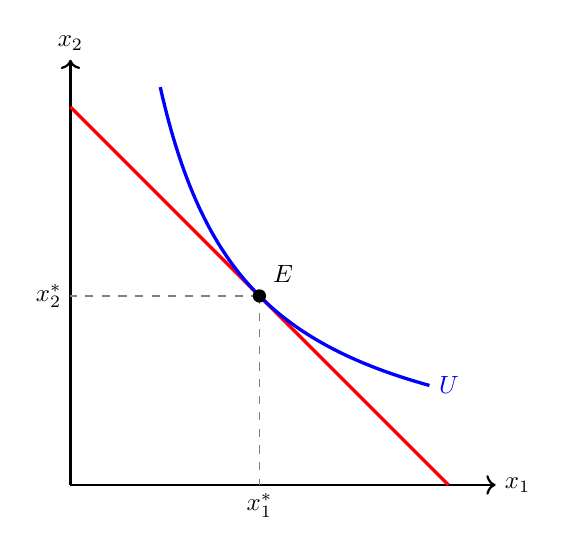
\begin{tikzpicture}[scale=1.2, every node/.style={scale=0.9}]
					% 坐标轴
					\draw[->, thick] (0,0) -- (4.5,0) node[right] {$x_1$};
					\draw[->, thick] (0,0) -- (0,4.5) node[above] {$x_2$};
					
					% 预算线: x1 + x2 = 4 (斜率为 -1)
					\draw[very thick, red] (0,4) -- (4,0);;
					
					% 无差异曲线: 使用 y = 4/x 确保在 (2,2) 处完美相切
					% domain 控制绘制范围，samples 保证曲线圆滑
					\draw[very thick, blue, domain=0.95:3.8, samples=100] 
					plot (\x, {4/\x}) node[right] {$U$};
					
					% 均衡点辅助虚线
					\draw[dashed, gray] (2,2) -- (2,0) node[below, black] {$x_1^*$};
					\draw[dashed, gray] (2,2) -- (0,2) node[left, black] {$x_2^*$};
					
					% 切点标注与防止遮挡
					\fill[black] (2,2) circle (2pt);
					\node[above right, xshift=2pt, yshift=2pt] at (2,2) {$E$};
					
				\end{tikzpicture}
			\end{center}
			\newpage
			\item \textbf{描述与互为完全替代品的两种商品相对应的无差异曲线。假如为完全互补品又怎么样呢？}
			
			\textbf{答：}
			
			1. 完全替代品：两种商品能够按照固定比例相互替代，其无差异曲线是一组相互平行、向右下方倾斜的直线，边际替代率恒定不变。
			
			2. 完全互补品：两种商品必须按照固定搭配比例一同消费，无法单独替代，对应的无差异曲线呈现直角弯折（L型）形态，直角的拐点代表最优搭配的消费组合。
			
			\begin{center}
				\begin{tikzpicture}[scale=1.1, every node/.style={scale=0.9}]
					% --- 左图：完全替代品 ---
					\begin{scope}[xshift=0cm]
						\draw[->] (0,0) -- (3.5,0) node[right] {\text{商品 }$1$};
						\draw[->] (0,0) -- (0,3.5) node[above] {\text{商品 }$2$};
						
						% 修改了节点位置：通过 anchor 和适度偏移，将 U1, U2, U3 整体向上提，避免与横轴重叠
						\draw[thick, blue] (0,2.5) -- (2.5,0) node[anchor=south west, xshift=-9pt, yshift=2pt] {$U_3$};
						\draw[thick, blue] (0,1.8) -- (1.8,0) node[anchor=south west, xshift=-9pt, yshift=2pt] {$U_2$};
						\draw[thick, blue] (0,1.1) -- (1.1,0) node[anchor=south west, xshift=-9pt, yshift=2pt] {$U_1$};
						
						\node[below] at (1.75,-0.5) {(a) 完全替代品};
					\end{scope}
					
					% --- 右图：完全互补品 ---
					\begin{scope}[xshift=6cm]
						\draw[->] (0,0) -- (3.5,0) node[right] {\text{商品 }$1$};
						\draw[->] (0,0) -- (0,3.5) node[above] {\text{商品 }$2$};
						
						% L型无差异曲线
						\draw[thick, red] (1.0,3.0) -- (1.0,1.0) -- (3.0,1.0) node[right] {$U_1$};
						\draw[thick, red] (1.7,3.0) -- (1.7,1.7) -- (3.0,1.7) node[right] {$U_2$};
						\draw[thick, red] (2.4,3.0) -- (2.4,2.4) -- (3.0,2.4) node[right] {$U_3$};
						
						% 拐点射线（固定搭配比例）
						\draw[dashed, gray] (0,0) -- (3.0,3.0);
						
						\node[below] at (1.75,-0.5) {(b) 完全互补品};
					\end{scope}
				\end{tikzpicture}
			\end{center}
			
			\item \textbf{序数效用和基数效用的区别是什么？解释对消费者选择进行排序时为什么不需要基数效用的假定。}
			
			\textbf{答：}
			
			序数效用与基数效用的核心区别在于对“效用是否可以量化”的认知不同。
			
			基数效用论认为，效用是可以具体量化和精确度量的。就像长度有“米”、重量有“千克”一样，效用也可以用明确的绝对数值（如 10 个效用单位）来表示满足程度的高低。这种理论主要采用边际效用分析法来研究消费者行为。
			
			序数效用论则认为，效用只是一种主观心理感受，无法精准量化。在现实中，消费者只需要也能对不同商品组合的偏好程度进行相对高低的“排序”（比如第一、第二、第三），而不需要明确知道具体高出多少数值。该理论主要使用无差异曲线与预算线作为核心分析工具。
			
			在对消费者选择进行分析时，之所以不需要基数效用的假定，是因为基数效用依赖的主观数值度量在现实中缺乏统一且客观的衡量标准，理论显得不够严谨。只要明确消费者对不同商品组合的偏好次序（即能判断出“更喜欢 A 还是 B”，或者“两者无差异”），就可以画出完整的无差异曲线。结合预算约束，这已经足够推导出消费者的最优选择和需求规律。由于序数效用足以完成全部的逻辑推导，且更加贴合人们现实的决策直觉，因此经济学就不再需要引入复杂且难以证伪的基数效用假定了。
			
			\newpage
			\item \textbf{画一条预算线，然后再画一条无差异曲线来说明与两种商品相对应的满足最大化选择。利用图形回答下述问题：\\ a. 假定其中一种商品实施配给。解释为什么消费者的境况可能变坏。\\ b. 假定其中一种商品被固定在当前市场价格以下水平，因此消费者不能想买多少就买多少。你能判断消费者的境况是变好了还是变坏了吗？}
			
			\textbf{答：}
			
			在没有任何限制的市场中，消费者通过寻找无差异曲线和预算线的切点来实现效用最大化。
			
			a.配给对福利的影响：当政府设置配给额度$\bar{x}_1$时，预算线会从配给点处垂直弯折，如果消费者原先的最优消费量超出了该额度，那么其可以得到的消费组合集将成为原来那个额度下的一个真子集。这样消费者不能停留在原来的最优无差异曲线上面，而是必须向左下方移动去寻找新的次优均衡点。由于新的最优决策点意味着更低水平的无差异曲线使消费者的总体效用降低，因此他们变坏。
			
			b.最高限价与短缺的不确定性：最高限价使商品的价格下降，预算线也随之变得更加平缓，增加了消费者的潜在购买力，但由于低廉的供给造成了供给短缺的存在，结果就是消费者的实际消费量被限定在供给配额$x_s$内。如果限价带来的收入足够弥补由购买限制导致的效用损失，那么消费者的福利水平可能提升；相反如果供给限制非常严厉，消费者的最好消费将极易偏离自己的喜好轨迹，使自身境况甚至比限价前还糟糕。所以限价政策对消费者产生的影响依赖于供给短缺程度的大小。
			
			\begin{center}
				\begin{tikzpicture}[scale=0.8, every node/.style={scale=0.75}]
					% --- 图 (a): 商品配给 (境况变坏) ---
					\begin{scope}[xshift=0cm]
						\draw[->] (0,0) -- (4,0) node[right] {$x_1$};
						\draw[->] (0,0) -- (0,4) node[above] {$x_2$};
						% 原预算线: x + y = 3
						\draw[dashed, gray] (0,3) -- (3,0);
						% 原均衡点: xy = 2.25 (1.5, 1.5)
						\draw[thick, blue!40, domain=0.8:2.8] plot (\x, {2.25/\x}) node[above] {$U_0$};
						\fill (1.5,1.5) circle (2pt) node[above right] {$E_0$};
						% 现在的预算线：配给 x=1。转折点 (1, 2)
						\draw[very thick, red] (0,3) -- (1,2); 
						\draw[very thick, red] (1,2) -- (1,0);   
						\draw[dashed, red] (1,2) -- (3,0);   
						\node[red, below] at (1,0) {$\bar{x}_1$};
						% 新均衡点: 落在垂直线上 (1, 2)。U = xy = 2
						\draw[thick, blue, domain=0.6:2.8] plot (\x, {2/\x}) node[right] {$U_R$};
						\fill (1,2) circle (2pt) node[above right] {$E_R$};
						\node[below] at (2,-0.8) {(a) 配给};
					\end{scope}
					
					% --- 图 (b): 最高限价 (境况变好) ---
					\begin{scope}[xshift=5.2cm]
						\draw[->] (0,0) -- (4,0) node[right] {$x_1$};
						\draw[->] (0,0) -- (0,4) node[above] {$x_2$};
						% 原预算线: x + y = 2.5。均衡 xy = 1.5625
						\draw[gray] (0,2.5) -- (2.5,0);
						\draw[thick, blue!30] plot[domain=0.7:2.4] (\x, {1.56/\x});
						\fill (1.25,1.25) circle (1.8pt) node[below left] {$E_0$};
						% 限价后预算线: 0.5x + y = 2.5。x_s = 2 时, y = 1.5。转折点 (2, 1.5)
						\draw[very thick, red] (0,2.5) -- (2,1.5); 
						\draw[very thick, red] (2,1.5) -- (2,0);   
						\draw[dashed, red] (2,1.5) -- (5,0);  
						\node[red, below] at (2,0) {$x_s$};
						% 新均衡点: (2, 1.5)。U = xy = 3
						\fill (2,1.5) circle (2pt) node[above right] {$E_1$};
						\draw[thick, blue] plot[domain=1.1:3.2] (\x, {3/\x}) node[right] {$U_1$};
						\node[below] at (2,-0.8) {(b) 限价：福利改善};
					\end{scope}
					
					% --- 图 (c): 最高限价 (境况变差) ---
					\begin{scope}[xshift=10.4cm]
						\draw[->] (0,0) -- (4,0) node[right] {$x_1$};
						\draw[->] (0,0) -- (0,4) node[above] {$x_2$};
						% 原预算线同上
						\draw[gray] (0,2.5) -- (2.5,0);
						\draw[thick, blue!30] plot[domain=0.7:2.9] (\x, {1.56/\x});
						\fill (1.25,1.25) circle (1.8pt) node[above right,yshift=-5pt] {$E_0$};
						% 限价同上。但供给极度匮乏: x_s = 0.5。转折点 (0.5, 2.25)
						\draw[very thick, red] (0,2.5) -- (0.5,2.25); 
						\draw[very thick, red] (0.5,2.25) -- (0.5,0); 
						\draw[dashed, red] (0.5,2.25) -- (5,0);   
						\node[red, below] at (0.5,0) {$x_s$};
						% 新均衡点: (0.5, 2.25)。U = xy = 1.125
						\fill (0.5,2.25) circle (2pt) node[above right] {$E_2$};
						\draw[thick, blue, domain=0.3:2.9] plot (\x, {1.12/\x}) node[right] {$U_2$};
						\node[below] at (2,-0.8) {(c) 限价：福利受损};
					\end{scope}
				\end{tikzpicture}
			\end{center}
			
			\newpage
			\item \textbf{描述边际相等原则。解释一下，为什么如果一种或两种商品的消费具有递增的边际效用，这一原则可能并不成立。}
			
			\textbf{答：}
			
			1. 边际相等原则：这是消费者效用最大化的核心准则。它指的是在收入与商品价格既定的条件下，消费者最优消费组合必须满足：两种商品的边际替代率等于商品的价格之比，这也等价于花费在每一种商品上的最后一单位货币所获得的边际效用彼此相等。其数学表达式如下：

				$$MRS_{12} = \frac{P_1}{P_2} = \frac{MU_1}{MU_2} \implies \frac{MU_1}{P_1} = \frac{MU_2}{P_2} = \lambda$$

			其中 $\lambda$ 为货币的边际效用。在此条件下，消费者无法通过调整消费组合进一步提升总效用，从而达到均衡状态。
			
			2. 边际效用递增时原则失效的原因：常规商品满足边际效用递减规律，存在内点最优解，因此边际相等原则成立。但如果商品存在边际效用递增的特征（例如成瘾性物品），消费者增加消费量时，额外获得的边际效用会持续上升。此时，消费者会产生不断加大单一商品消费的动机，其最优选择通常为角点解（即将其全部收入集中用于购买边际效用递增的商品），不再遵循将消费均等分配的等边际规则。因此，在这种情况下，边际相等原则不再成立。
			
			\begin{center}
				\begin{tikzpicture}[scale=1.2, every node/.style={scale=0.9}]
					% --- 左图：正常商品 (凸向原点，内点解) ---
					\begin{scope}[xshift=0cm]
						% 坐标轴
						\draw[->, thick] (0,0) -- (4,0) node[right] {商品 $1$};
						\draw[->, thick] (0,0) -- (0,4) node[above] {商品 $2$};
						
						% 预算线: x + y = 3
						\draw[thick, red] (0,3) -- (3,0);;
						
						% 无差异曲线 (凸向原点) 
						\draw[very thick, blue, domain=0.75:3.4, samples=100] 
						plot (\x, {2.25/\x}) node[right] {$U_1$};
						
						% 均衡点标注
						\fill (1.5,1.5) circle (2pt);
						\node[above right, xshift=2pt] at (1.5,1.5) {$E$};
						
						\node[below] at (1.75,-0.6) {(a) 边际效用递减};
					\end{scope}
					
					% --- 右图：成瘾商品 (凹向原点，角点解) ---
					\begin{scope}[xshift=6cm]
						% 坐标轴
						\draw[->, thick] (0,0) -- (4,0) node[right] {普通商品};
						\draw[->, thick] (0,0) -- (0,4) node[above] {成瘾商品};
						
						% 预算线: x + y = 3
						\draw[thick, red] (0,3) -- (3,0);
						
						% 较低的无差异曲线 (切点效用极小)
						% 使用 arc 画完美圆弧：半径 sqrt(4.5) ≈ 2.1213，确保严丝合缝
						\draw[thick, blue!40] (2.1213,0) arc (0:90:2.1213);
						\node[blue!40] at (2.3, 0.4) {$U_1$};
						
						\fill[gray] (1.5,1.5) circle (1.5pt);
						\node[above right, xshift=0pt, yshift=-2pt, gray] at (1.5,1.5) { $E'$ };
						
						% 较高的无差异曲线 (角点效用极大)
						% 使用 arc 画完美圆弧：半径 3，完美连接 (3,0) 和 (0,3)
						\draw[very thick, blue] (3,0) arc (0:90:3);
						\node[blue] at (3.3, 0.4) {$U_2$};
						
						% 角点解标注 (全部收入购买成瘾商品)
						\fill[red] (0,3) circle (2.5pt);
						\node[right, xshift=1pt, yshift=6pt] at (0,3) {$E^*$ （最优点）};
						
						\node[below] at (1.75,-0.6) {(b) 边际效用递增};
					\end{scope}
				\end{tikzpicture}
			\end{center}
			\newpage
			\item \textbf{在过去20年中计算机的价格已经大幅下跌。请用这一价格下跌的情况解释为什么消费者价格指数可能在很大程度上高估了那些密集使用计算机的人的生活成本指数。}
			
			\textbf{答：}
			
			消费者价格指数（CPI）本质上是一种拉氏价格指数，它采用固定基期的商品消费篮子来计算价格变动。这种计算方式存在两类系统性偏误，导致其在面对计算机价格大幅下跌时，会高估密集使用计算机人群的真实生活成本：
			
			1. 替代偏误：拉氏指数固定了基期的消费篮子，没有考虑消费者的替代行为。在计算机价格大幅下跌后，消费者理性的选择是增加计算机的购买量，以替代其他价格相对更高的商品。然而，CPI 仍然以基期的固定权重进行计算，无法反映消费者通过调整消费结构所带来的成本节约，因此高估了实际的生活成本。
			
			2. 质量变化偏误：CPI 未能充分核算商品质量的提升。在过去20年中，计算机价格下跌的同时，其性能、算力和功能等质量指标出现了飞跃式的提升。CPI 往往将这种质量提升带来的巨大效用增益，误判为单纯的商品价格下降，从而低估了消费者的真实购买力，这也进一步导致了对生活成本的高估。
			
			\item \textbf{解释为什么帕氏指数通常会低估理想生活成本指数。}
			
			\textbf{答：}
			
			1. 核心定义：
			帕氏指数是以当期消费组合为权重的价格指数，即用当期价格购买当期组合的成本，与基期价格购买当期组合的成本之比。其核心计算公式如下：

				$$\text{帕氏指数} = \frac{\sum P_t Q_t}{\sum P_0 Q_t}$$

			相对而言，理想生活成本指数是指以当期价格实现基期效用水平所需的最小成本，与基期实现该效用的成本之比。
			
			2. 低估原因：
			帕氏指数采用当期消费组合 $Q_t$ 作为权重，而 $Q_t$ 是消费者在当期价格下，已经根据价格变动完成了消费替代（即减少购买涨价商品、增加购买降价商品）之后的最终结果。这种替代行为自然压低了涨价商品在总消费中的权重，使得帕氏指数计算出的成本变化，低于消费者“维持基期效用不变”所需要面临的真实成本变化。因此，帕氏指数通常会系统性地低估理想生活成本指数。
		\end{enumerate}
		\newpage
	\section{练习题}
		\begin{enumerate}[label=\textbf{\arabic*.}, leftmargin=*]		
			\item \textbf{在本章中，对于不同商品的消费者偏好在分析中没有发生变化。不过在有些情况下，消费时偏好的确会变化。讨论一下，就消费下述这两种商品而言，偏好为什么以及怎样在一段时间后可能会变化。\\ a. 卷烟；\\b. 在一家有特色菜肴的餐厅里初次用餐。}
			
			\textbf{答：}
			
			a. 卷烟为成瘾性商品，消费后尼古丁依赖增强，边际效用递增，对卷烟的偏好随消费次数增加而持续增强。
			
			b. 特色餐厅初次用餐为体验品，偏好随体验结果变化：体验良好则偏好正向增强，体验不佳则偏好减弱甚至消失。
			
			\begin{center}
				\begin{tikzpicture}[scale=0.8, every node/.style={scale=0.8}]
					% --- 图 (a)：卷烟 (偏好增强) ---
					\begin{scope}[xshift=0cm]
						\draw[->, thick] (0,0) -- (3.5,0) node[right] {卷烟};
						\draw[->, thick] (0,0) -- (0,3.5) node[above] {其他商品};
						% 初始 U1
						\draw[thick, gray] (0.5,2.5) -- (2.5,0.5);
						\node[gray, right, fill=white, inner sep=1pt] at (2.5,0.5) {$U_1$};
						% 变动后 U2 (更陡)
						\draw[thick, red, dashed] (0.5,3.0) -- (2.2,0.3);
						\node[red, right, yshift=5pt, fill=white, inner sep=1pt] at (1.5,0.3) {$U_2$};
						\node[below] at (1.75,-0.6) {\textbf{(a) 卷烟：偏好增强}};
					\end{scope}
					
					% --- 图 (b)：餐厅 (体验良好 -> 偏好增强) ---
					\begin{scope}[xshift=5.8cm]
						\draw[->, thick] (0,0) -- (3.5,0) node[right] {餐厅};
						\draw[->, thick] (0,0) -- (0,3.5) node[above] {其他};
						% 初始 U1
						\draw[thick, gray] (0.5,2.5) -- (2.5,0.5);
						\node[gray, right, fill=white, inner sep=1pt] at (2.5,0.5) {$U_1$};
						% 变动后 U2 (斜率变陡，标注上移)
						\draw[thick, blue, dashed] (0.5,3.2) -- (2.0,0.8);
						\node[blue, right, yshift=8pt, fill=white, inner sep=1pt] at (1.7,1.4) {$U_2$};
						\node[below] at (1.75,-0.6) {\textbf{(b) 餐厅：体验良好}};
					\end{scope}
					
					% --- 图 (c)：餐厅 (体验不佳 -> 偏好减弱) ---
					\begin{scope}[xshift=11.6cm]
						\draw[->, thick] (0,0) -- (3.5,0) node[right] {餐厅};
						\draw[->, thick] (0,0) -- (0,3.5) node[above] {其他};
						% 初始 U1
						\draw[thick, gray] (0.5,2.5) -- (2.5,0.5);
						\node[gray, right, fill=white, inner sep=1pt] at (2,1.5) {$U_1$};
						% 变动后 U2 (斜率变平缓，标注上移)
						\draw[thick, red, dashed] (0.5,1.8) -- (3.2,0.2);
						\node[red, right, yshift=8pt, fill=white, inner sep=1pt] at (3.2,0.2) {$U_2$};
						\node[below] at (1.75,-0.6) {\textbf{(c) 餐厅：体验不佳}};
					\end{scope}
				\end{tikzpicture}
			\end{center}
		
			\item \textbf{画出下述两种商品个人偏好的无差异曲线：汉堡包和软饮料。指出个人满足（或效用）增加的方向。\\ a. 乔的无差异曲线为凸的，汉堡包和软饮料都不喜欢。\\ b. 简喜欢汉堡包，但不喜欢软饮料。如果服务员给她一份软饮料，她会不喝倒掉。\\ c. 鲍勃喜欢汉堡包，但不喜欢软饮料。但是如果服务员给他一份软饮料，为了礼貌起见他会喝掉。\\ d. 莫利喜欢汉堡包和软饮料，但坚持精确地按照两个汉堡包搭配一份软饮料来吃。\\ e. 比尔喜欢汉堡包，但对软饮料无所谓喜欢或不喜欢。\\ f. 玛丽从额外一份汉堡包中获得的满足是从额外一份软饮料中所获得满足的两倍。}
			
			\textbf{答：}
			
			a. 两者均为厌物品，无差异曲线凸向原点，效用向原点方向（左下方）增加。
			
			b. 软饮料为厌物品，汉堡包为喜好品。无差异曲线向右上方倾斜，效用随汉堡增加、软饮料减少（向右下方）而增加。
			
			c. 同 b，软饮料对其依然产生负效用（需要强迫自己喝掉），无差异曲线向右上方倾斜，效用向右下方增加。
			
			d. 汉堡与软饮料为完全互补品，无差异曲线为直角形，直角拐点在 $H = 2S$ 射线上，效用向右上方增加。
			
			e. 软饮料为中性商品，无差异曲线为垂直于汉堡包轴的直线（若汉堡在横轴则为垂直线，若在纵轴则为水平线。本图示将其置于纵轴则为水平线，效用向右方增加）。
			
			f. 汉堡与软饮料为完全替代品，无差异曲线为斜率恒定的直线，斜率绝对值为 $1/2$（横轴为汉堡时），效用向右上方增加。
			
			\begin{center}
				\begin{tikzpicture}[scale=0.8, every node/.style={scale=0.85}]
					% ==================== 第一行 ====================
					
					% --- a. 乔：双厌物品 ---
					\begin{scope}[xshift=0cm, yshift=0cm]
						\draw[->, thick] (0,0) -- (3.5,0) node[right] {汉堡};
						\draw[->, thick] (0,0) -- (0,3.5) node[above] {软饮};
						
						% U1 (外侧，效用较低)
						\draw[thick, blue, domain=0.8:2.8, samples=50] plot (\x, {2.25/\x}) node[right] {$U_1$};
						% U2 (内侧，效用较高，靠近原点)
						\draw[thick, blue, domain=0.4:2.5, samples=50] plot (\x, {1/\x}) node[below,xshift=8pt,yshift=5pt] {$U_2$};
						
						% 效用增加箭头 (严格在两线之间，向左下方)
						\draw[->, red, thick] (1.3, 1.3) -- (1.1, 1.1);
						
						\node[below] at (1.75,-0.6) {(a) 乔：都讨厌};
					\end{scope}
					
					% --- b. 简：厌软饮 ---
					\begin{scope}[xshift=5.2cm, yshift=0cm]
						\draw[->, thick] (0,0) -- (3.5,0) node[right] {汉堡};
						\draw[->, thick] (0,0) -- (0,3.5) node[above] {软饮};
						
						% U1 (左上方，效用较低)
						\draw[thick, blue] (0.5, 1.5) -- (2.0, 3.0) node[right] {$U_1$};
						% U2 (右下方，效用较高)
						\draw[thick, blue] (1.5, 0.5) -- (3.0, 2.0) node[right] {$U_2$};
						
						% 效用增加箭头 (严格在两线之间，向右下方)
						\draw[->, red, thick] (1.2, 1.9) -- (1.9, 1.2);
						
						\node[below] at (1.75,-0.6) {(b) 简：讨厌软饮};
					\end{scope}
					
					% --- c. 鲍勃：厌软饮 ---
					\begin{scope}[xshift=10.4cm, yshift=0cm]
						\draw[->, thick] (0,0) -- (3.5,0) node[right] {汉堡};
						\draw[->, thick] (0,0) -- (0,3.5) node[above] {软饮};
						
						% U1 (左上方，效用较低)
						\draw[thick, blue] (0.5, 1.5) -- (2.0, 3.0) node[right] {$U_1$};
						% U2 (右下方，效用较高)
						\draw[thick, blue] (1.5, 0.5) -- (3.0, 2.0) node[right] {$U_2$};
						
						% 效用增加箭头 (严格在两线之间，向右下方)
						\draw[->, red, thick] (1.2, 1.9) -- (1.9, 1.2);
						
						\node[below] at (1.75,-0.6) {(c) 鲍勃：讨厌软饮};
					\end{scope}
					
					% ==================== 第二行 ====================
					% 增大 yshift 的负值（从 -4.5cm 改为 -6.0cm），彻底避免与第一行重叠
					
					% --- d. 莫利：完全互补 ---
					\begin{scope}[xshift=0cm, yshift=-6.0cm]
						\draw[->, thick] (0,0) -- (3.5,0) node[right] {汉堡};
						\draw[->, thick] (0,0) -- (0,3.5) node[above] {软饮};
						
						% 比例射线
						\draw[dashed, gray] (0,0) -- (2.5,1.25);
						
						% U1 (靠近原点)
						\draw[thick, blue] (0.8, 2.5) -- (0.8, 0.4) -- (2.5, 0.4) node[right] {$U_1$};
						% U2 (远离原点)
						\draw[thick, blue] (1.6, 2.5) -- (1.6, 0.8) -- (2.5, 0.8) node[right] {$U_2$};
						
						% 效用增加箭头 (沿比例射线向右上方)
						\draw[->, red, thick] (1.1, 0.55) -- (1.4, 0.7) ;
						
						\node[below] at (1.75,-0.6) {(d) 莫利：完全互补};
					\end{scope}
					
					% --- e. 比尔：中性商品 ---
					\begin{scope}[xshift=5.2cm, yshift=-6.0cm]
						\draw[->, thick] (0,0) -- (3.5,0) node[right] {汉堡};
						\draw[->, thick] (0,0) -- (0,3.5) node[above] {软饮};
						
						% U1 (靠左)
						\draw[thick, blue] (1.0, 0) -- (1.0, 2.8) node[above] {$U_1$};
						% U2 (靠右)
						\draw[thick, blue] (2.0, 0) -- (2.0, 2.8) node[above] {$U_2$};
						
						% 效用增加箭头 (向右方)
						\draw[->, red, thick] (1.2, 1.5) -- (1.8, 1.5) ;
						
						\node[below] at (1.75,-0.6) {(e) 比尔：中性商品};
					\end{scope}
					
					% --- f. 玛丽：完全替代 ---
					\begin{scope}[xshift=10.4cm, yshift=-6.0cm]
						\draw[->, thick] (0,0) -- (3.5,0) node[right] {汉堡};
						\draw[->, thick] (0,0) -- (0,3.5) node[above] {软饮};
						
						% U1 (靠近原点，斜率为 -2)
						\draw[thick, blue] (0, 2.0) -- (2.0, 0) node[right,xshift=-2pt,yshift=6pt] {$U_1$};
						% U2 (远离原点，斜率为 -2)
						\draw[thick, blue] (0, 3.0) -- (3, 0) node[right,xshift=-4pt,yshift=9pt] {$U_2$};
						
						% 效用增加箭头 (向右上方)
						\draw[->, red, thick] (1, 1) -- (1.45, 1.45);		
						\node[below] at (1.75,-0.6) {(f) 玛丽：完全替代};
					\end{scope}
				\end{tikzpicture}
			\end{center}
			
			\item \textbf{假如简目前愿意以4张电影票来换取1张篮球赛门票，那么与电影相比，她肯定更喜欢篮球。这一说法是对还是错？请解释。}
			
			\textbf{答：}
			
			该说法错误。
			
			边际替代率（$MRS$）反映的仅仅是消费者在特定消费组合下的边际意愿：
				$$MRS = \frac{MU_{\text{篮球}}}{MU_{\text{电影}}} = 4$$
			这仅说明在现有持有量下，额外 $1$ 张篮球赛门票带来的边际效用是 $1$ 张电影票的 $4$ 倍，不能等同于她整体更喜欢篮球。根据边际效用递减规律，如果简当前手里有大量电影票而几乎没有篮球票，电影票的边际效用会被拉低，自然愿意用多张电影票换 $1$ 张篮球票，这种高边际替代率是由初始资源禀赋决定的，而非绝对偏好排序。此外，她愿意换票也不一定是因为喜欢篮球运动本身，可能是为了陪同亲友、观看赛场偶像等衍生需求，这些因素同样会提高篮球票对她的边际效用。因此，仅凭边际交换意愿无法判定她与电影相比更喜欢篮球，题干说法不成立。
			
			\begin{center}
				\begin{tikzpicture}[scale=1.2, every node/.style={scale=0.9}]
					% 坐标轴
					\draw[->, thick] (0,0) -- (4.5,0) node[right] {电影票};
					\draw[->, thick] (0,0) -- (0,4.5) node[above] {篮球门票};
					
					% 无差异曲线 (y = 2/x)
					\draw[very thick, blue, domain=0.55:4, samples=100] 
					plot (\x, {2/\x}) node[right, fill=white, inner sep=1pt] {$U$};
					
					% 切线标注与延长 (在 x=3 处，斜率约为 -0.22)
					% 为了视觉平衡，绘制一段较长的切线
					\draw[dashed, red, thick] (1.5, 1.0) -- (4.2, 0.4);
					
					% 切点 A 及其标注
					\fill[black] (3.0, 0.67) circle (2pt);
					\node[above right, fill=white, inner sep=1pt, yshift=3pt] at (3.0, 0.67) {$A$ (此处 $MRS=4$)};
					
	
					
				\end{tikzpicture}
			\end{center}
			
			\item \textbf{加内勒和布赖恩每个人计划花费20000美元在汽车的款式和油耗这两个性能上。他们可以选择款式，也可以选择油耗，或者是两者的组合。加内勒对款式无所谓，但是希望油耗尽可能地低。布赖恩对两者的喜欢程度相同，想在每样性能上花费相同数额的钱。利用无差异曲线和预算线，说明两人各将做怎样的选择。}
			
			\textbf{答：}
			
			加内勒：款式对她而言是中性商品，她仅偏好低油耗（即高燃油经济性）。因此，她的无差异曲线是水平线。她的最优选择是角点解，即将全部 $20000$ 美元预算用于购买高燃油经济性，而在款式上的支出为 $0$。
			
			布赖恩：款式与燃油经济性对他而言是完全替代品，且偏好程度等同。如果两者价格一致，他的最优选择是内点解，比如在款式和燃油经济性上各花费 $10000$ 美元。
			
			\begin{center}
				\begin{tikzpicture}[scale=1.1, every node/.style={scale=0.9}]
					% --- 左图：加内勒 (款式中性，偏好低油耗) ---
					\begin{scope}[xshift=1.2cm]
						\draw[->, thick] (0,0) -- (3.5,0) node[right] {款式};
						\draw[->, thick] (0,0) -- (0,3.5) node[above] {燃油经济性};
						
						% 预算线
						\draw[very thick, black] (0,3) -- (3,0);
						
						% 无差异曲线族 (水平线)
						\draw[thick, blue] (0,1.8) -- (3.2,1.8) node[right] {$U_1$};
						\draw[thick, blue] (0,3) -- (3.2,3) node[right] {$U_2$};
						
						% 效用增加箭头 (添加文字说明，避免空箭头)
						\draw[->, red, thick] (2.2, 2.0) -- (2.2, 2.8);
						
						% 均衡点标注
						\fill[red] (0,3) circle (2.5pt);
						\node[left, xshift=-4pt, fill=white, inner sep=1pt] at (0,3) {最优解 (角点)};
						
						\node[below] at (1.75,-0.7) {\textbf{(a) 加内勒：单方面偏好}};
					\end{scope}
					
					% --- 右图：布赖恩 (完全替代且均等消费) ---
					\begin{scope}[xshift=8cm]
						\draw[->, thick] (0,0) -- (4,0) node[right] {款式};
						\draw[->, thick] (0,0) -- (0,4) node[above] {燃油经济性};
						
						% 预算线
						\draw[very thick, black] (0,3) -- (3,0);
						
						% 支出相等线 (y=x)
						\draw[dashed, gray!80, thick] (0,0) -- (3.2,3.2);
						
						% 无差异曲线 U1
						\draw[thick, blue] (0,1.5) -- (1.5,0) node[right, font=\footnotesize, fill=white,yshift=9pt,xshift=-1pt] {$U_1$};
						
						% 最优无差异曲线 U2 (与预算线重合)
						\draw[thick, blue] (0,3) -- (3,0);
						\node[blue, above right, fill=white, inner sep=1pt] at (2.2,0.9) {$U_2$ （和预算线重合）};
						
						% 效用增加箭头 (添加文字说明)
						\draw[->, red, thick] (0.8, 0.8) -- (1.2, 1.2);
						
						% 投影虚线
						\draw[dashed, gray] (1.5,0) node[below, black] {\small 10000} -- (1.5,1.5) -- (0,1.5) node[left, black] {\small 10000};
						
						% 均衡点及文字标注 (修复点：补全了 {} 及其中的内容)
						\fill[red] (1.5,1.5) circle (2.5pt);
						
						\node[below] at (1.75,-0.7) {\textbf{(b) 布赖恩：均衡偏好}};
					\end{scope}
				\end{tikzpicture}
			\end{center}
			
			\item \textbf{假如布里奇特和艾玲的收入花在两种商品上——食品（$F$）和衣服（$C$）。布里奇特的偏好效用函数 $U(F, C) = 10FC$ 表示，而艾玲的偏好用效用函数 $U(F, C) = 0.20F^2C^2$ 表示。\\ a. 以食品为横轴，以衣服为纵轴，在图上找到能给予布里奇特与组合（10，5）相同效用水平的点集。在另一幅图上为艾玲找到相同的点集。\\ b. 在同样两幅图中，分别找出能给予布里奇特和艾玲与组合（15，8）一样效用水平的点集。\\ c. 你认为布里奇特和艾玲的偏好相同吗？请解释。}
			
			\textbf{答：}
			
			a. 对于组合 $(10, 5)$：
	
				布里奇特的效用为 $U_B = 10 \times 10 \times 5 = 500$，无差异曲线方程为 $FC = 50$。\\
				艾玲的效用为 $U_E = 0.20 \times 10^2 \times 5^2 = 500$，无差异曲线方程同样为 $FC = 50$。
	
			二者在此组合下的点集完全重合。
			
			b. 对于组合 $(15, 8)$：
	
				布里奇特的效用为 $U_B = 10 \times 15 \times 8 = 1200$，无差异曲线方程为 $FC = 120$。\\
				艾玲的效用为 $U_E = 0.20 \times 15^2 \times 8^2 = 2880$，无差异曲线方程化简后同样为 $FC = 120$。
	
			二者在此组合下的点集依然完全重合。
			\newpage
			c. 布里奇特和艾玲的偏好完全相同。
	
				$$U_E = 0.20(FC)^2 = 0.20 \left(\frac{U_B}{10}\right)^2 = 0.002 U_B^2$$
	
			由于 $U_B > 0$，艾玲的效用函数是布里奇特效用函数的严格正单调变换。序数效用论认为，效用函数的绝对数值并不重要，只要单调性一致，它们所反映的商品组合的排序偏好以及无差异曲线族就是完全相同的。
			
			\begin{center}
				\begin{tikzpicture}[scale=1.1, every node/.style={scale=0.9}]
					% --- 左图：组合 (10, 5) ---
					\begin{scope}[xshift=0cm]
						\draw[->, thick] (0,0) -- (4,0) node[right] {\text{食品 }$F$};
						\draw[->, thick] (0,0) -- (0,4) node[above] {\text{衣服 }$C$};
						
						\draw[very thick, blue, domain=0.4:3.5, samples=100] plot (\x, {1.5/\x});
						
						\fill (1.5,1.0) circle (2pt);
						\node[above right] at (1.5,1.0) {$(10,5)$};
						\node[below] at (2,-0.5) {\text{点集 }$FC=50$};
					\end{scope}
					
					% --- 右图：组合 (15, 8) ---
					\begin{scope}[xshift=6cm]
						\draw[->, thick] (0,0) -- (4,0) node[right] {\text{食品 }$F$};
						\draw[->, thick] (0,0) -- (0,4) node[above] {\text{衣服 }$C$};
						
						\draw[very thick, red, domain=0.8:3.8, samples=100] plot (\x, {3.0/\x});
						
						\fill (2.0,1.5) circle (2pt);
						\node[above right] at (2.0,1.5) {$(15,8)$};
						\node[below] at (2,-0.5) {\text{点集 }$FC=120$};
					\end{scope}
				\end{tikzpicture}
			\end{center}
			
			\item \textbf{假设琼斯和史密斯已决定每年花1000美元在曲棍球赛或摇滚音乐会这两种形式的娱乐上。他们都喜欢这两种商品，将会选择消费正数量的这两种商品。但对这两种形式的娱乐，琼斯和史密斯在他们的偏好方面分歧很大，琼斯更偏好曲棍球赛，而史密斯则更偏好摇滚音乐会。\\ a. 为琼斯画一组无差异曲线，为史密斯画第二组曲线。\\ b. 运用边际替代率概念解释为什么这两组曲线彼此不一样。}
			
			\textbf{答：}
			
			a. 设横轴为摇滚音乐会场次 $R$，纵轴为曲棍球赛场次 $H$。琼斯更偏好曲棍球赛，史密斯更偏好摇滚音乐会，两人的无差异曲线特征如下：
			
			\begin{center}
				\begin{tikzpicture}[scale=1.1, every node/.style={scale=0.9}]
					% --- 琼斯的无差异曲线 (偏好 H，曲线较平缓) ---
					\begin{scope}[xshift=0cm]
						\draw[->, thick] (0,0) -- (4.5,0) node[right] {\text{摇滚音乐会} $R$};
						\draw[->, thick] (0,0) -- (0,4.5) node[above] {\text{曲棍球赛} $H$};
						
						\draw[very thick, blue] plot[smooth, tension=0.8] coordinates {(0.5, 2.5) (1.5, 1.5) (3.5, 0.8)};
						\node[right, blue] at (3.5, 0.8) {$U_1$};
						
						\draw[very thick, blue] plot[smooth, tension=0.8] coordinates {(0.8, 3.5) (2.0, 2.2) (4.0, 1.4)};
						\node[right, blue] at (4.0, 1.4) {$U_2$};
						
						\node[below] at (2.25,-0.6) {\textbf{(a) 琼斯：偏好曲棍球（平缓）}};
					\end{scope}
					
					% --- 史密斯的无差异曲线 (偏好 R，曲线较陡峭) ---
					\begin{scope}[xshift=6.5cm]
						\draw[->, thick] (0,0) -- (4.5,0) node[right] {\text{摇滚音乐会} $R$};
						\draw[->, thick] (0,0) -- (0,4.5) node[above] {\text{曲棍球赛} $H$};
						
						\draw[very thick, red] plot[smooth, tension=0.8] coordinates {(0.5, 3.5) (1.0, 1.5) (2.5, 0.5)};
						\node[right, red] at (2.5, 0.5) {$U_1$};
						
						\draw[very thick, red] plot[smooth, tension=0.8] coordinates {(1.0, 4.2) (1.6, 2.4) (3.5, 1.0)};
						\node[right, red] at (3.5, 1.0) {$U_2$};
						
						\node[below] at (2.25,-0.6) {\textbf{(b) 史密斯：偏好摇滚（陡峭）}};
					\end{scope}
				\end{tikzpicture}
			\end{center}
			
			b. 边际替代率（$MRS$）的定义为消费者在保持总效用不变的前提下，为多获得一单位某种商品而愿意放弃的另一种商品的数量。在本题中：
	
				$$MRS_{RH} = - \frac{\Delta H}{\Delta R}$$
	
			此公式表示为多获得 1 单位摇滚音乐会（$R$），愿意放弃的曲棍球赛（$H$）的数量，在几何上等于无差异曲线斜率的绝对值。
	
			对于琼斯：他更偏好曲棍球赛，因此曲棍球赛对他来说边际效用很高。为了让他放弃 1 单位的曲棍球赛，需要给他大量的摇滚音乐会作为补偿。反过来说，他愿意为增加 1 单位摇滚音乐会而放弃的曲棍球赛数量极少，即 $MRS_{RH}$ 较小，导致其无差异曲线平缓。\\
			对于史密斯：他更偏好摇滚音乐会。他愿意放弃大量的曲棍球赛来换取额外的 1 单位摇滚音乐会，即 $MRS_{RH}$ 较大，导致其无差异曲线较陡峭。
	
			\item \textbf{DVD的价格（$D$）是20美元，CD的价格（$C$）是10美元。菲利普有一笔100美元的预算，可以花在这两种商品上。假设他已购买了1张DVD和1张CD。另外，他其实还想再购买3张DVD和5张CD。\\ a. 在上述价格和收入下，以横轴表示CD，画出菲利普的预算约束。\\ b. 考虑菲利普已经购买的和仍然想要购买的这两种商品，找出他可以购买的三个不同的CD与DVD的组合。假定他只能购买整数单位。}
			
			\textbf{答：}
			
			a. 菲利普的预算约束方程为：

				$$20D + 10C = 100 \implies 2D + C = 10$$
			
			\begin{center}
				\begin{tikzpicture}[scale=1.1, every node/.style={scale=0.9}]
					\draw[->, thick] (0,0) -- (6,0) node[right] {$CD$};
					\draw[->, thick] (0,0) -- (0,4) node[above] {$DVD$};
					
					% 预算线: 2D + C = 10 -> 如果 C=10(放x轴), D=5(放y轴)
					% 比例设为 1单位 = 0.5cm
					\draw[very thick, blue] (5,0) node[below, black] {$10$} -- (0,2.5) node[left, black] {$5$};
					
					% 已购买组合 (1,1) -> 坐标 (0.5, 0.5)
					\fill[black] (0.5, 0.5) circle (2pt);
					\node[right, fill=white, inner sep=1pt] at (0.8, 0.5) {\text{已购买 } $(1,1)$};

					\fill[red] (3, 2) circle (2pt);
					\node[above right, fill=white, inner sep=1pt] at (3.1, 2) {计划购买$(6,4)$};
				\end{tikzpicture}
			\end{center}
			
			b. 他想要的总购买量为 $6$ 张 CD 和 $4$ 张 DVD，总花费将达到 $6 \times 10 + 4 \times 20 = 140$ 美元，显然超出了 $100$ 美元的预算约束。由于他已经购买了 $1$ 张 DVD 和 $1$ 张 CD（花费 $30$ 美元），剩余预算为 $70$ 美元。
			满足预算且数量为整数的可行组合如下表：
			
			\begin{center}
				\begin{tabularx}{0.8\textwidth}{>{\centering\arraybackslash}X >{\centering\arraybackslash}X >{\centering\arraybackslash}X}
					\toprule
					\textbf{CD 数量 ($C$)} & \textbf{DVD 数量 ($D$)} & \textbf{总花费 (美元)} \\
					\midrule
					8 & 1 & $8 \times 10 + 1 \times 20 = 100$ \\
					6 & 2 & $6 \times 10 + 2 \times 20 = 100$ \\
					4 & 3 & $4 \times 10 + 3 \times 20 = 100$ \\
					2 & 4 & $2 \times 10 + 4 \times 20 = 100$ \\
					\bottomrule
				\end{tabularx}
			\end{center}
			
			\newpage
			\item \textbf{安妮的工作要求她每四个星期中有三个星期要外出，假定她有一个年交通预算，可以乘火车或者坐飞机。她经常去的航空公司实施了一个里程积分项目，根据她的飞行里程对机票价格打折。当她一年内的飞行里程达到25000英里之后，航空公司在该年的剩余时间里对机票减价25\%；达到50000英里之后，减价50\%。以纵轴表示火车里程数，以横轴表示飞行里程数，画出安妮的预算线。}
			
			\textbf{答：}
			
			本题的核心在于分析价格折扣如何通过改变“相对价格比”来影响预算线的斜率。
   				$$ P_{F}F+P_{T}T=M $$
				$$ k = - \frac{P_{F}}{P_{T}}$$
			
			斜率代表了安妮多飞行 1 英里的“机会成本”，即她必须放弃的火车旅行英里数。随着飞行里程增加并触发折扣，飞行价格 $P_{F}$ 会分阶段下降，导致预算线在不同的里程关口发生“转折”：
			
			1. 0 至 25000 英里阶段：飞行价格为原价 $P_F$。此时预算线最陡峭，机会成本最高。\\
			2. 25000 至 50000 英里阶段：飞行价格降为 $0.75P_F$。由于分子变小，斜率的绝对值减小，预算线在 25000 英里处发生转折并变得平缓。\\
			3. 50000 英里以上阶段：飞行价格降为 $0.5P_F$。机会成本进一步降低，预算线在 50000 英里处第二次转折，变为最平缓的一段。
			
			最终，安妮面临的是一条由三段斜率不同的线段组成的、向外凸出的折线预算线。
			\begin{center}
				\begin{tikzpicture}[scale=0.75, every node/.style={scale=0.85}]
					\draw[->, thick] (0,0) -- (8,0) node[right] {\text{飞行里程 }$F$};
					\draw[->, thick] (0,0) -- (0,5.5) node[above] {\text{火车里程 }$T$};
					
					% 设定坐标点代表不同阶段的折扣
					% 0-25000: 原价 (较陡)
					\draw[very thick, blue] (0, 5) node[left, black] {$M/P_T$} -- (2.5, 3.5);
					\node[above right, rotate=-30] at (1.25, 4.25) {\text{原价}};
					
					% 25000-50000: 75折 (变平缓)
					\draw[very thick, blue] (2.5, 3.5) -- (5.0, 2.375);
					\node[above right, rotate=-24] at (3.75, 2.9375) {\text{75折}};
					
					% >50000: 5折 (最平缓)
					\draw[very thick, blue] (5.0, 2.375) -- (8.0, 1.25);
					\node[above right, rotate=-20] at (6.5, 1.8125) {\text{5折}};
					
					% 辅助虚线与坐标轴标记
					\draw[dashed, gray] (2.5, 0) node[below, black] {$25000$} -- (2.5, 3.5);
					\draw[dashed, gray] (5.0, 0) node[below, black] {$50000$} -- (5.0, 2.375);
				\end{tikzpicture}
			\end{center}
			
			\newpage
			\item \textbf{黛布拉去电影院的时候常常会购买软饮料，她有三个选择：8盎司的饮料要价1.50美元，12盎司的饮料要价2.00美元，16盎司的饮料要价2.25美元。画出黛布拉购买饮料时面临的预算约束。（假定黛布拉处理她不需要的软饮料时无须花费成本。）}
			
			\textbf{答：}
			
			非线性定价（数量折扣）通过改变价格比来影响预算线的斜率。
			
			设纵轴为其他商品 $Y$（假设单价 $P_Y = 1$ 美元），横轴为饮料盎司数 $Q$，总预算为 $M$。预算方程和斜率可表示为：
			$$ P_{Q}Q + Y = M $$
			$$ k = - \frac{P_{Q}}{P_{Y}} = - P_{Q} $$
			
			斜率代表了黛布拉多购买 1 盎司软饮料的“机会成本”，即她必须放弃的其他商品的价值（美元）。随着购买容量的增加，软饮料的边际价格 $P_Q$ 分阶段下降，导致预算线在不同的容量关口发生“转折”：
			
			1. 0 至 8 盎司阶段：总花费 1.50 美元，边际价格为 $1.50 / 8 = 0.1875$ 美元/盎司。此时预算线最陡峭，机会成本最高。\\
			2. 8 至 12 盎司阶段：增加 4 盎司需额外花费 0.50 美元，边际价格降为 $0.50 / 4 = 0.125$ 美元/盎司。由于边际价格变小，斜率的绝对值减小，预算线在 8 盎司处发生转折并变得平缓。\\
			3. 12 至 16 盎司阶段：增加 4 盎司仅需额外花费 0.25 美元，边际价格进一步降为 $0.25 / 4 = 0.0625$ 美元/盎司。机会成本最低，预算线在 12 盎司处第二次转折，变为最平缓的一段。
			
			最终，黛布拉面临的是一条由三段斜率不同的线段组成的、向外凸出的折线预算线。
			
			\begin{center}
				\begin{tikzpicture}[scale=1.2, every node/.style={scale=0.9}]
					% 坐标轴
					\draw[->, thick] (0,0) -- (6,0) node[right] {\text{饮料盎司数 }$Q$};
					\draw[->, thick] (0,0) -- (0,4.2) node[above] {\text{其他商品 }$Y$};
					
					% 预算线绘制 (纯净版，无多余文字)
					\draw[very thick, blue] (0, 3.5) node[left, black] {$M$} -- (2, 2.0);
					\draw[very thick, blue] (2, 2.0) -- (3, 1.5);
					\draw[very thick, blue] (3, 1.5) -- (4, 1.25);
					
					% 辅助虚线与横轴标记 (容量)
					\draw[dashed, gray] (2, 2.0) -- (2, 0) node[below, black] {$8$};
					\draw[dashed, gray] (3, 1.5) -- (3, 0) node[below, black] {$12$};
					\draw[dashed, gray] (4, 1.25) -- (4, 0) node[below, black] {$16$};
					
					% 辅助虚线与纵轴标记 (剩余预算直观表达)
					\draw[dashed, gray] (2, 2.0) -- (0, 2.0) node[left, black] {$M-1.50$};
					\draw[dashed, gray] (3, 1.5) -- (0, 1.5) node[left, black] {$M-2.00$};
					\draw[dashed, gray] (4, 1.25) -- (0, 1.25) node[left, black] {$M-2.25$};
					
					% 拐点强调
					\fill[red] (2, 2.0) circle (1.5pt);
					\fill[red] (3, 1.5) circle (1.5pt);
				\end{tikzpicture}
			\end{center}
			
			\newpage
			\item \textbf{安东尼奥在读大一时买了5本大学新教材，每本花了80美元。而二手教材每本只卖50美元。当书店宣布新教材涨价10\%、旧教材涨价5\%的时候，安东尼奥的父亲多给了他40美元。\\ a. 安东尼奥的预算线如何变动？以纵轴表示新教材进行说明。\\ b. 在价格变动之后，安东尼奥的境况是变好了还是变坏了？请解释。}
			
			\textbf{答：}
			
			a. 初始状态下，新教材（$N$）价格为 $80$ 美元，二手教材（$U$）价格为 $50$ 美元，总预算 $M = 5 \times 80 = 400$ 美元。
			涨价后，新教材价格变为 $88$ 美元，二手教材变为 $52.5$ 美元。由于父亲多给了 $40$ 美元，新预算为 $440$ 美元。
			
				$$ \text{原预算线：} 80N + 50U = 400 $$
				$$ \text{新预算线：} 88N + 52.5U = 440 $$
			
			计算可知，由于新增的补助恰好抵消了新教材的涨价成本，两条预算线的纵轴截距相同（均为 $N=5$）。但新预算线的横轴截距（$U \approx 8.38$）大于原横轴截距（$U=8$），预算线绕纵轴截距点向外旋转。
			
			\begin{center}
				\begin{tikzpicture}[scale=0.75, every node/.style={scale=0.85}]
					% 坐标轴
					\draw[->, thick] (0,0) -- (7.5,0) node[right] {\text{二手教材 }$U$};
					\draw[->, thick] (0,0) -- (0,6.5) node[above] {\text{新教材 }$N$};
					
					% 预算线 (视觉缩放比例: 原横轴截距8->4.5, 新横轴截距8.38->6.5)
					\draw[thick, dashed, gray] (0, 5) -- (4.5, 0) node[below, black] {$8$};
					\draw[very thick, blue] (0, 5) -- (6.5, 0) node[below, black] {$8.38$};
					
					% A点: 纵轴截距点 (价格变化旋转中心)
					\fill[black] (0,5) circle (1.5pt) node[left] {$5$};
					\node[above right] at (0,5) {$A$};
					
					% C点: 原最优选择 (内部切点，取 U=3.15, N=1.5)
					\coordinate (C) at (3.15, 1.5);
					\fill[red] (C) circle (2pt);
					\node[above right, black, fill=white, inner sep=1pt] at (C) {$C$};
					\draw[dashed, gray] (3.15, 0) node[below, black] {$U_C$} -- (C) -- (0, 1.5) node[left, black] {$N_C$};
					
					% B点: 新最优选择 (内部切点，取 U=3.9, N=2.0)
					% 严格满足 C 点在 B 点左下方的要求 (3.15 < 3.9 且 1.5 < 2.0)
					\coordinate (B) at (3.9, 2.0);
					\fill[red] (B) circle (2pt);
					\node[above right, black, fill=white, inner sep=1pt] at (B) {$B$};
					\draw[dashed, gray] (3.9, 0) node[below, black] {$U_B$} -- (B) -- (0, 2.0) node[left, black] {$N_B$};
					
					% 无差异曲线 IC1: 
					% 使用反比例函数，在 C(3.15, 1.5) 处与原预算线精确相切 (原预算线斜率为 -5/4.5 = -1.111)
					\draw[thick, orange, domain=0.8:4.2, samples=100] plot (\x, {27.77/(\x + 1.85) - 4.054});
					\node[orange, right] at (4.2, 0.5) {$IC_1$};
					
					% 无差异曲线 IC2: 
					% 使用反比例函数，在 B(3.9, 2.0) 处与新预算线精确相切 (新预算线斜率为 -5/6.5 = -0.769)
					\draw[thick, red, domain=1.0:6.0, samples=100] plot (\x, {19.225/(\x + 1.1) - 1.845});
					\node[red, right] at (6.0, 0.8) {$IC_2$};
				\end{tikzpicture}
			\end{center}
			
			b. 安东尼奥的境况变好了。
			
			新的预算约束完全覆盖了原来的消费组合（$5$ 本新教材、$0$ 本旧教材），这保证了他的效用底线不会下降。同时，新旧教材的相对价格发生改变，预算空间向外扩张。由于二手教材的相对价格变得更便宜，他可以通过减少新教材购买、增加二手教材购买，从而触及一条比原来更高水平的无差异曲线（从 $IC_1$ 提升至 $IC_2$），实现整体福利的改善。
			
			\item\textbf{在佐治亚，鳄梨的价格是桃子的两倍。不过，在加利福尼亚，两者的价格是一样的。假如两州的消费者都最大化了其效用，对他们来说，桃子对鳄梨的边际替代率是否相同？如果不同，哪个州的消费者该值更高？}
			
			\textbf{答：}
			令商品1=桃子，商品2=鳄梨。
			
			效用最大化时，消费者的边际替代率等于两种商品的价格之比：
				$$MRS_{12} = \frac{MU_1}{MU_2} = \frac{P_1}{P_2}$$
			
			佐治亚州：$P_2=2P_1$，因此
			$$MRS_{12} = \frac{P_1}{P_2} = \frac{1}{2}$$
			
			加利福尼亚州：$P_2=P_1$，因此
			$$MRS_{12} = \frac{P_1}{P_2} = 1$$
			
			两州消费者的边际替代率不相同，加利福尼亚州消费者的桃子对鳄梨的边际替代率更高。
			
			\item \textbf{本在两种商品间分配其预算：比萨饼和墨西哥玉米煎饼。
				a. 以横轴表示比萨饼，用图说明本的最优组合。
				b. 假定现在对比萨饼收税，使得其价格上涨了20\%，说明本现在的最优组合。
				c. 假定比萨饼现在实行配给制，在本要求的数量以下，说明此时的最优组合。}
			
			\textbf{答：}

			a. 初始最优组合：预算线与最高无差异曲线的切点 $E_1$ 即为最优消费组合，此时 $MRS_{XY}=P_X/P_Y$。
			
			b. 价格上涨后的最优组合：预算线绕纵轴向内旋转至 $AB'$，与更低的无差异曲线相切于 $E_2$。比萨饼消费量减少，效用水平下降。
			
			c. 配给制下的最优组合：配给量 $X_R$ 小于初始最优消费量，最优组合为预算线与配给线的交点 $E_3$，此时无差异曲线与预算线相交而非相切，效用水平低于初始最优。
			
			\begin{center}
				\begin{tikzpicture}[scale=0.85, every node/.style={scale=0.9}]
					
					% --- 图 (a): 初始最优组合 (相切均衡) ---
					\begin{scope}[xshift=0cm]
						\draw[->, thick] (0,0) -- (4.2,0) node[right] {$X$};
						\draw[->, thick] (0,0) -- (0,4.2) node[above] {$Y$};
						
						% 预算线: x + y = 3.5
						\draw[thick, black] (0,3.5) node[left] {$A$} -- (3.5,0) node[below] {$B$};
						
						% 无差异曲线 U1: y = 3.0625/x (在 1.75, 1.75 处完美相切)
						\draw[thick, blue, domain=0.85:3.8, samples=100] plot (\x, {3.0625/\x}) node[right] {$U_1$};
						
						% 最优点 E1
						\fill (1.75, 1.75) circle (2pt);
						\node[above right] at (1.75, 1.75) {$E_1$};
						
						\node[below] at (1.75,-0.6) {(a) 初始最优组合};
					\end{scope}
					
					% --- 图 (b): 价格上涨后的最优组合 (斜率变陡，切点左移) ---
					\begin{scope}[xshift=5.8cm]
						\draw[->, thick] (0,0) -- (4.2,0) node[right] {$X$};
						\draw[->, thick] (0,0) -- (0,4.2) node[above] {$Y$};
						
						% 原预算线 (参考) 与 新预算线 (更陡)
						\draw[thick, dashed, gray!60] (0,3.5) -- (3.5,0);
						\draw[thick, black] (0,3.5) node[left] {$A$} -- (2.1,0) node[below] {$B'$};
						
						% 原无差异曲线 U1 (参考)
						\draw[thick, blue!30, domain=1.0:3.8, samples=100] plot (\x, {3.0625/\x})
						node[right,xshift=-25pt,yshift=15pt] {$U_1$};
						
						% 新无差异曲线 U2: y = 1.9/x (在约 1.07, 1.71 处与新线相切)
						\draw[thick, blue, domain=0.6:3.5, samples=100] plot (\x, {1.85/\x}) node[right] {$U_2$};
						
						% 最优点 E2
						\fill (1.07, 1.73) circle (2pt);
						\node[above right] at (0.6, 1.0) {$E_2$};
						
						\node[below] at (1.75,-0.6) {(b) 价格上涨后的最优组合};
					\end{scope}
					
					% --- 图 (c): 配给制下的最优组合 (角点解/非相切) ---
					\begin{scope}[xshift=11.6cm]
						\draw[->, thick] (0,0) -- (4.2,0) node[right] {$X$};
						\draw[->, thick] (0,0) -- (0,4.2) node[above] {$Y$};
						
						% 预算线 (参考)
						\draw[thick, dashed, gray!60] (0,3.5) -- (3.5,0);
						% 配给制预算线: 在 X_R 处垂直
						\draw[thick, black] (0,3.5) node[left] {$A$} -- (1.2, 2.3);
						\draw[thick, black] (1.2, 2.3) -- (1.2, 0) node[below] {$X_R$};
						
						% 穿过配给点 (1.2, 2.3) 的无差异曲线 U2: y = 2.76/x
						\draw[thick, blue, domain=0.8:3.5, samples=100] plot (\x, {2.76/\x}) node[right] {$U_2$};
						% 原无差异曲线 U1 (更高，不可达)
						\draw[thick, blue!30, domain=1.0:3.5, samples=100] plot (\x, {3.0625/\x}) node[right,xshift=-25pt,yshift=15pt] {$U_1$};
						
						% 配给均衡点 E3 (在转折角上)
						\fill (1.2, 2.3) circle (2pt);
						\node[above right] at (1.2, 2.3) {$E_3$};
						
						\node[below] at (1.75,-0.6) {(c) 配给制下的最优组合};
					\end{scope}
					
				\end{tikzpicture}
			\end{center}
			
				\item \textbf{题目：布伦达打算购买新汽车，预算为25000美元。她新近发现了一本杂志，该杂志给每辆汽车就款式和油耗分别赋予一个指数，指数的区间为1\textasciitilde10，10代表最好的款式或者最低的油耗。通过观察汽车清单，她发现款式指数每上升一单位，汽车的价格就上升5000美元。她还发现，油耗指数每下降一单位，汽车的价格就上升2500美元。\\
					a. 以横轴表示油耗，说明布伦达在25000美元的预算下所能选择的款式（$S$）和油耗（$G$）的各种组合。\\
					b. 假定布伦达的偏好是这样的，即她从额外一单位款式中获得的满足总是从油耗中获得的三倍。布伦达将选择什么样的汽车？\\
					c. 假定布伦达的边际替代率（油耗对款式）等于 $S/(4G)$。她希望她的汽车的各项指数为多少呢？\\
					d. 假定布伦达的边际替代率（油耗对款式）等于 $3S/G$。她希望她的汽车的各项指数为多少呢？}
				
				\textbf{答：}
				
				\textbf{a.} 设款式指数为 $S$，油耗指数为 $G$（指数越高，油耗表现越差，即价格越低）。由题意可知，款式价格 $P_S = 5000$ 美元/单位；油耗价格 $P_G = -2500$ 美元/单位。
				
				$$ 5000S - 2500G = 25000 \implies 2S - G = 10 $$
				
				同时，指数存在客观的取值范围约束：$S, G \in [1, 10]$。布伦达在预算下的选择组合如下图所示：
				
				\begin{center}
					\begin{tikzpicture}[scale=0.55, >=stealth, every node/.style={scale=0.9}]
						% 坐标轴
						\draw[->, thick] (0,0) -- (11.5,0) node[right] {$G$};
						\draw[->, thick] (0,0) -- (0,11.5) node[above] {$S$};
						
						% 预算线 (2S - G = 10)
						\draw[very thick, black] (1, 5.5) -- (10, 10);
						
						% 约束点标注
						\fill[black] (1, 5.5) circle (2pt);
						\node[below right] at (1, 5.5) {$(1, 5.5)$};
						\fill[black] (10, 10) circle (2pt);
						\node[above left] at (10, 10) {$(10, 10)$};
						
						% 辅助虚线
						\draw[dashed, gray] (1,0) node[below, black] {$1$} -- (1,5.5) -- (0,5.5) node[left, black] {$5.5$};
						\draw[dashed, gray] (10,0) node[below, black] {$10$} -- (10,10) -- (0,10) node[left, black] {$10$};
					\end{tikzpicture}
				\end{center}
				
				\textbf{b.} 效用函数为 $U = 3S + G$，此时边际替代率为恒定常数：
				$$ MRS_{G,S} = \frac{1}{3} $$
				由于边际替代率小于价格比：
				$$ MRS_{G,S} < \frac{P_G}{P_S} $$
				说明款式的边际效用相对更高，消费者倾向于将全部预算用于购买款式。结合变量取值下限，最优解为角点解：
				$$ G = 1, \quad S = 5.5 $$
				
				\textbf{c.} 当 $MRS_{G,S} = S/(4G)$ 时，效用最大化条件要求 $MRS_{G,S} = P_G/P_S$：
				$$ \frac{S}{4G} = \frac{1}{2} \implies S = 2G $$
				代入预算方程 $2S - G = 10$ 中，解得：
				$$ G = \frac{10}{3}, \quad S = \frac{20}{3} $$
				
				\textbf{d.} 当 $MRS_{G,S} = 3S/G$ 时，效用最大化条件要求：
				$$ \frac{3S}{G} = \frac{1}{2} \implies G = 6S $$
				代入预算方程 $2S - G = 10$ 中，解得：
				$$ S = -2.5 $$
				该结果不符合 $S \ge 1$ 的客观约束，超出可行范围。此时对于消费者而言，油耗的边际效用极高，最优解必然发生在边界处，即角点解：
				$$ S = 10, \quad G = 10 $$
				
				\item \textbf{康妮每月将200美元的收入用于购买两种商品：肉和土豆。\\
					a. 假设肉每磅是4美元，土豆每磅是2美元，画出她的预算约束。\\
					b. 再假设她的效用函数由方程 $U(M,P)=2M+P$ 给出，她应该购买哪种肉和土豆的组合以使其效用最大化？（提示：肉和土豆是完全替代品。）\\
					c. 康妮去的超市有一项特价促销活动，如果她购买20磅土豆（每磅2美元），超市就免费再赠送她10磅土豆，这一赠送只限于她购买的最初20磅土豆。超过最初20磅以上的所有土豆（除了奖励的土豆之外）仍然是每磅2美元。画出她的预算约束。\\
					d. 假设一场使土豆腐烂的病害的爆发将土豆的价格抬至每磅4美元。超市结束了其促销活动。康妮现在的预算约束又会是怎样的呢？哪种肉和土豆的组合使其效用最大化？}
				
				\textbf{答：}
				
				\begin{center}
					\begin{tikzpicture}[scale=0.7, every node/.style={scale=0.8}]
						\begin{scope}[xshift=0cm]
							\draw[->, thick] (0,0) -- (6.0,0) node[right] {$P$};
							\draw[->, thick] (0,0) -- (0,6.0) node[above] {$M$};
							% 比例：M缩放为1/10 (50->5)，P缩放为1/20 (100->5)
							\draw[very thick, black] (0,5) node[left] {$50$} -- (5,0) node[below] {$100$};
							% 无差异曲线重合
							\draw[thick, blue, dashed] (0,5) -- (5,0) node[pos=0.8, above right] {$U_1$};
							\node[below] at (2.5, -0.8) {(1) 初始预算约束};
						\end{scope}

					\begin{scope}[xshift=8cm]
						\draw[->, thick] (0,0) -- (6.5,0) node[right] {$P$};
						\draw[->, thick] (0,0) -- (0,6.0) node[above] {$M$};
						% 预算线折线
						\draw[very thick, black] (0,5) node[left] {$50$} -- (1,4) -- (1.5,4) -- (5.5,0) node[below] {$110$};
						% 辅助线
						\draw[dashed, gray] (1,0) node[below, black] {$20$} -- (1,4) -- (0,4) node[left, black] {$40$};
						\draw[dashed, gray] (1.5,0) node[below, black] {$30$} -- (1.5,4);
						% 无差异曲线 U=110
						\draw[thick, blue, dashed] (0,5.5) -- (5.5,0) node[pos=0.2, above right] {$U_2=110$};
						\fill[red] (1.5,4) circle (2.5pt) node[above right] {$E$};
						\node[below] at (3.25, -0.8) {(2) 促销后的预算约束};
					\end{scope}
					
					\begin{scope}[xshift=16cm]
						\draw[->, thick] (0,0) -- (4.0,0) node[right] {$P$};
						\draw[->, thick] (0,0) -- (0,6.0) node[above] {$M$};
						% 新预算线 M=50-P
						\draw[very thick, black] (0,5) node[left] {$50$} -- (2.5,0) node[below] {$50$};
						% 无差异曲线 MRS=0.5 (较平缓)
						\draw[thick, blue, dashed] (0,5) -- (5,2.5) node[right] {$U_3$};
						\fill[red] (0,5) circle (2.5pt) node[right, xshift=2pt,yshift=5pt] {$E^*$};
						\node[below] at (2.0, -0.8) {(3) 价格上涨后的角点解};
					\end{scope}
					\end{tikzpicture}
				\end{center}
				
				\textbf{a.} 初始预算方程为：
				$$ 2M + P = 100 $$
				
				\textbf{b.} 对于完全替代品，其边际替代率为：
				$$ MRS_{P,M} = \frac{MU_P}{MU_M} = \frac{1}{2} $$
				由于此时边际替代率恰好等于市场价格比：
				$$ \frac{P_P}{P_M} = \frac{1}{2} $$
				康妮在预算线上的任何一点都能获得相同的最大化效用，即满足以下方程的任意 $(P, M)$ 组合均为最优解：
				$$ 2M + P = 100 $$
				
				\textbf{c.} 促销活动使得预算线变为非线性的折线，分为三个阶段：
					1. 当 $0 \le P \le 20$ 时，为正常价格阶段，方程为：
					$$ M = 50 - 0.5P $$
					2.当 $20 < P \le 30$ 时，为免费获赠阶段，不消耗额外预算，方程为：
					$$ M = 40 $$
					3.当 $P > 30$ 时，恢复原价阶段，继续购买需支付每磅 2 美元，方程为：
					$$ 4M + 2(P-10) = 200 \implies M = 55 - 0.5P $$
				
				\textbf{d.} 土豆涨价至 4 美元/磅后，新预算方程变为：
				$$ 4M + 4P = 200 \implies M = 50 - P $$
				此时边际替代率与价格比的关系为：
				$$ MRS_{P,M} = \frac{1}{2} < \frac{P_P}{P_M} = 1 $$
				这说明肉的相对边际效用高于其相对价格。效用最大化的结果是角点解，即康妮会将全部 200 美元用于购买肉：
				$$ M = 50, \quad P = 0 $$
				
				
				
				\item \textbf{简从国内旅游的天数（$D$）和国外旅游的天数（$F$）中获得效用，由效用函数 $U(D,F)=10DF$ 给出。另外，在国内旅游每天的价格为100美元，在国外旅游每天的价格为400美元，简旅游的年预算为4000美元。\\
					a. 分别说明与效用水平800和1200相对应的无差异曲线。\\
					b. 在同一幅图上画出简的预算线。\\
					c. 简有能力购买能给她800效用的组合吗？1200呢？\\
					d. 求简实现效用最大化时国内旅游的天数和国外旅游的天数的选择。}
				
				\textbf{答：}
				
				\begin{center}
					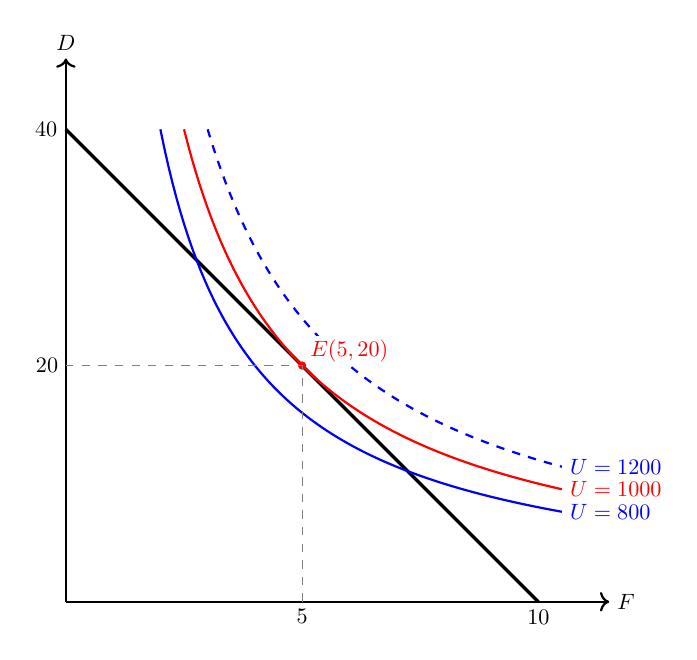
\begin{tikzpicture}[scale=0.6, every node/.style={scale=0.8}]
						\draw[->, thick] (0,0) -- (11.5,0) node[right] {$F$};
						\draw[->, thick] (0,0) -- (0,11.5) node[above] {$D$};
						
						% 缩放设定：纵轴 D 缩放为 1/4 (40->10)
						% 预算线 (y = 10 - x)
						\draw[very thick, black] (0,10) node[left] {$40$} -- (10,0) node[below] {$10$};
						
						% U=800 无差异曲线 (y' = 20/x)
						\draw[thick, blue, domain=2.0:10.5, samples=100] plot (\x, {20/\x}) node[right] {$U=800$};
						
						% U=1200 无差异曲线 (y' = 30/x)
						\draw[thick, blue, dashed, domain=3.0:10.5, samples=100] plot (\x, {30/\x}) node[right] {$U=1200$};
						
						% 最大效用 U=1000 无差异曲线，精确相切于 (5, 5) 对应实际的 (F=5, D=20)
						\draw[thick, red, domain=2.5:10.5, samples=100] plot (\x, {25/\x}) node[right] {$U=1000$};
						
						% 相切均衡点
						\fill[red] (5,5) circle (2.5pt);
						\node[above right, red, fill=white, inner sep=1.5pt,xshift=2pt] at (5,5) {$E(5, 20)$};
						
						% 辅助虚线
						\draw[dashed, gray] (5,0) node[below, black] {$5$} -- (5,5) -- (0,5) node[left, black] {$20$};
					\end{tikzpicture}
				\end{center}
				
				\textbf{a.} 根据效用函数，无差异曲线的数学表达式为：
				$$ U = 800 \implies 10DF = 800 \implies D = \frac{80}{F} $$
				$$ U = 1200 \implies 10DF = 1200 \implies D = \frac{120}{F} $$
				两者均为严格凸向原点的反比例双曲线，效用值为 1200 的曲线位于效用值为 800 的曲线的右上方。
				
				\textbf{b.} 预算约束方程为 $100D + 400F = 4000 \implies D = 40 - 4F$。
				
				\textbf{c.} 将预算线代入无差异曲线进行判断：
				由于最优效用发生在预算线与某条无差异曲线相切处，我们可以在 (d) 问中求得简能实现的最大效用为 $U = 1000$。
				因此，800 效用的无差异曲线与预算线有交点（例如 $D=20, F=4$），简有能力购买；而 1200 效用的曲线完全在预算线之外，简无法负担。
				
				\textbf{d.} 根据效用最大化的切点条件，边际替代率等于价格比：
				$$ MRS_{F,D} = \frac{MU_F}{MU_D} = \frac{D}{F} $$
				$$ \frac{D}{F} = \frac{P_F}{P_D} = 4 \implies D = 4F $$
				将其代入预算方程 $D + 4F = 40$，解得 $F = 5, D = 20$。最优组合为国内旅游 20 天，国外旅游 5 天。

				\item \textbf{朱利奥从消费食品（$F$）和衣服（$C$）中获得效用，由效用函数 $U(F,C)=FC$ 给出。另外，食品的价格为每单位2美元，衣服的价格为每单位10美元，朱利奥每星期的收入为50美元。\\
					a. 当朱利奥实现效用最大化时，食品对衣服的边际替代率是多少？请解释。\\
					b. 假设与效用最大化时的组合相比，朱利奥多购买了食品，少购买了衣服，他的食品对衣服的边际替代率会大于还是小于a部分的答案？请解释。}
				
				\textbf{答：}
				
				\textbf{a.}消费者实现效用最大化时，边际替代率等于市场价格比：
				$$ MRS_{F,C} = \frac{MU_F}{MU_C} = \frac{P_F}{P_C} = \frac{1}{5} $$
				在最优消费点处，由于价格约束，朱利奥主观上愿意放弃 $1$ 单位的衣服来换取额外 $5$ 单位的食品，这恰好等同于市场上购买 $1$ 单位食品所需要付出的衣服的真实机会成本。
				
				\textbf{b.}对于效用函数 $U(F,C) = FC$，其食品对衣服的边际替代率为：
				$$ MRS_{F,C} = \frac{MU_F}{MU_C} = \frac{C}{F} $$
				当朱利奥沿预算线向右下方移动（即 $F$ 增加、$C$ 减少）时，比值 $C/F$ 的分子减小、分母增大，因此 $MRS_{F,C}$ 会小于$0.2$。
				
				这反映了边际替代率递减规律。随着食品消费量的增加，食品的边际效用$MU_F$降低；同时衣服数量的减少使得衣服变得更为稀缺，其边际效用$MU_C$升高。因此，为获得额外一单位食品，他愿意放弃的衣服数量会越来越少（无差异曲线变得更加平缓）。

				\begin{center}
					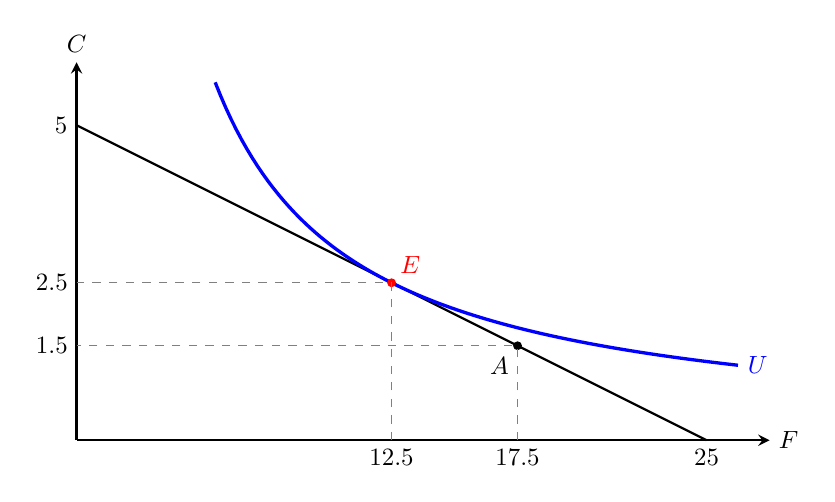
\begin{tikzpicture}[scale=0.8, >=stealth, every node/.style={scale=0.9}]

						\draw[->, thick] (0,0) -- (11,0) node[right] {$F$};
						\draw[->, thick] (0,0) -- (0,6) node[above] {$C$};

						\draw[thick, black] (0,5) node[left] {$5$} -- (10,0) node[below] {$25$};
						
						\draw[very thick, blue, domain=2.2:10.5, samples=100] plot (\x, {12.5/\x}) node[right] {$U$};
						
						\fill[red] (5,2.5) circle (2pt);
						\node[above right, red] at (5,2.5) {$E$};
						\draw[dashed, gray] (5,0) node[below, black] {$12.5$} -- (5,2.5) -- (0,2.5) node[left, black] {$2.5$};

						\fill[black] (7,1.5) circle (2pt);
						\node[above left,yshift=-15pt] at (7,1.5) {$A$};
						\draw[dashed, gray] (7,0) node[below, black] {$17.5$} -- (7,1.5) -- (0,1.5) node[left, black] {$1.5$};
					\end{tikzpicture}
				\end{center}
				
				\newpage
				\item \textbf{玛莉蒂斯从消费食品（$F$）和衣服（$C$）中得到的效用由 $U(F,C)=FC$ 给出。假设1990年她的收入为1200美元，食品和衣服的价格均为每单位1美元。但是到了2000年，食品价格上升至2美元，衣服价格上升至3美元。以100表示1990年的生活成本指数。请计算玛莉蒂斯在这样的偏好下，2000年的理想生活成本指数和拉氏指数。（提示：玛莉蒂斯将购买相同数量的食品和衣服。）}
				
				\textbf{答：}
				
				\textbf{1.计算基期（1990年）最优消费组合与效用水平}
				
				基期预算方程为 $F + C = 1200$。由效用最大化条件 $MRS_{F,C} = C/F = P_F/P_C = 1$，解得基期最优消费篮子为：
				$$ F_0 = 600, \quad C_0 = 600 $$
				玛莉蒂斯在基期获得的效用水平为：
				$$ U_0 = 600 \times 600 = 360000 $$
				
				\textbf{2.计算拉氏指数}
				
				拉氏指数采用基期的固定消费篮子 $(F_0, C_0)$ 作为权重，评估当期价格下购买该组合所需的成本涨幅：
				$$ \text{拉氏指数} = \frac{P_{F1}F_0 + P_{C1}C_0}{P_{F0}F_0 + P_{C0}C_0} \times 100 = \frac{2 \times 600 + 3 \times 600}{1200} \times 100 = 250 $$
				
				\textbf{3.计算理想生活成本指数}
				
				理想指数考量消费者为维持基期效用水平 $U_0 = 360000$ 不变时，在当期价格下所需的最小支出。
				在 2000 年的新价格下，最小化成本的切点条件为 $MRS_{F,C} = C/F = P_{F1}/P_{C1} = 2/3$，即 $C = 2F/3$。将其代入效用水平约束中：
				$$ F \times \left( \frac{2F}{3} \right) = 360000 \implies F_1 = 300\sqrt{6} \approx 734.85, \quad C_1 = 200\sqrt{6} \approx 489.90 $$
				维持该效用所需的当期最小总支出为：
				$$ E_1 = P_{F1}F_1 + P_{C1}C_1 = 2 \times 300\sqrt{6} + 3 \times 200\sqrt{6} \approx 2939.39 \text{ 美元} $$
				$$ \text{理想指数} = \frac{E_1}{E_0} \times 100 = \frac{2939.39}{1200} \times 100 \approx 245 $$
				
				拉氏指数为 250，理想生活成本指数约为 245。由于拉氏指数未能将消费者面对相对价格变化时进行的“消费替代行为”（用相对便宜的商品替代涨价商品）计算在内，它系统性地高估了真实的生活成本上升幅度。
		
		\end{enumerate}
	% =======================================================
	%                 第 4 章：个人需求与市场需求
	% =======================================================
	\chapter{个人需求与市场需求}
	
	\section{复习题}
	\begin{enumerate}[label=\textbf{\arabic*.}, leftmargin=*]
		\item \textbf{解释下面各项中每一项的区别：(1) 价格-消费曲线与需求曲线；(2) 个人需求曲线与市场需求曲线；(3) 收入-消费曲线与恩格尔曲线；(4) 收入效应与替代效应。}
		
		\textbf{答：}
		
		\textbf{(a) 价格-消费曲线 (PCC) 与需求曲线}
		
		价格-消费曲线是在消费者偏好、收入和其他商品价格不变的前提下，某一商品价格变动引起的效用最大化均衡点的轨迹，它反映了两种商品最优消费组合的变动路线。而需求曲线是由价格-消费曲线推导而来的，反映了单一商品需求量与其自身价格的一一对应关系，需求曲线上的每一点都满足效用最大化的均衡条件。
		\begin{center}
			\begin{tikzpicture}[scale=0.75, >=stealth, thick, every node/.style={scale=0.85}]
				% ==================== 左图：价格-消费曲线 (PCC) ====================
				\begin{scope}[xshift=0cm]
					% 横轴延长至9.5，防止标签重叠
					\draw[->] (0,0) -- (9.5,0) node[right] {$X$};
					\draw[->] (0,0) -- (0,5.5) node[above] {$Y$};
					
					% 预算线：假设 I=10, Py=2 (Y轴截距恒为5)
					% BL1: Px=2.5 (X截距=4)
					\draw[blue!60] (0,5) node[left, black] {$I/P_Y$} -- (4,0) node[below, black] {$P_{x1}$};
					% BL2: Px=1.66 (X截距=6)
					\draw[blue!60] (0,5) -- (6,0) node[below, black] {$P_{x2}$};
					% BL3: Px=1.11 (X截距=9)
					\draw[blue!60] (0,5) -- (9,0) node[below, black] {$P_{x3}$};
					
					% 均衡点：Y随X增加，使得PCC向右上方倾斜
					% E1: 在BL1上，选择 (2.0, 2.5)，斜率 m = 1.25
					\fill[black] (2.0, 2.5) circle (2pt) node[above right, fill=white, inner sep=1pt] {$E_1$};
					\draw[blue, domain=1.0:3.8, samples=100] plot (\x, {2.8125/(\x-0.5) + 0.625}) node[right] {$U_1$};
					
					% E2: 在BL2上，选择 (2.7, 2.75)，斜率 m = 5/6
					\fill[black] (2.7, 2.75) circle (2pt) node[above right, fill=white, inner sep=1pt] {$E_2$};
					\draw[blue, domain=1.6:5.0, samples=100] plot (\x, {(10/3)/(\x-0.7) + 13/12}) node[right] {$U_2$};
					
					% E3: 在BL3上，选择 (3.6, 3.0)，斜率 m = 5/9
					\fill[black] (3.6, 3.0) circle (2pt) node[above right, fill=white, inner sep=1pt] {$E_3$};
					\draw[blue, domain=2.2:7.5, samples=100] plot (\x, {4.05/(\x-0.9) + 1.5}) node[right] {$U_3$};
					
					% PCC 曲线：橙色，平滑连接且向右上方倾斜
					\draw[orange, dashed, ultra thick] plot[smooth] coordinates {(1.5, 2.1) (2.0, 2.5) (2.7, 2.75) (3.6, 3.0) (4.5, 3.25)} node[right, fill=white, inner sep=1pt] {PCC};
					
					% 辅助线
					\draw[dashed, gray] (2.0,0) -- (2.0, 2.5);
					\draw[dashed, gray] (2.7,0) -- (2.7, 2.75);
					\draw[dashed, gray] (3.6,0) -- (3.6, 3.0);
					
					\node[below] at (4.5,-1) {(a) 价格-消费曲线};
				\end{scope}
				
				% ==================== 右图：需求曲线推导 ====================
				\begin{scope}[xshift=11cm]
					\draw[->] (0,0) -- (9,0) node[right] {$Q_X$};
					\draw[->] (0,0) -- (0,5.5) node[above] {$P_X$};
					
					% 需求曲线：仅此线条为红色
					\draw[red, ultra thick] plot[smooth] coordinates {(1.2, 4.2) (2.0, 2.5) (2.7, 1.66) (3.6, 1.11) (6.0, 0.5)} node[right] {$D$};
					
					% 对应点：全黑
					\fill[black] (2.0, 2.5) circle (2pt) node[above right, fill=white, inner sep=1pt] {$E'_1$};
					\fill[black] (2.7, 1.66) circle (2pt) node[above right, fill=white, inner sep=1pt] {$E'_2$};
					\fill[black] (3.6, 1.11) circle (2pt) node[above right, fill=white, inner sep=1pt] {$E'_3$};
					
					% 辅助线与标注：黑色/灰色系
					\draw[dashed, gray] (2.0,0) node[below, black] {$X_1$} -- (2.0, 2.5) -- (0, 2.5) node[left, black] {$P_{x1}$};
					\draw[dashed, gray] (2.7,0) node[below, black] {$X_2$} -- (2.7, 1.66) -- (0, 1.66) node[left, black] {$P_{x2}$};
					\draw[dashed, gray] (3.6,0) node[below, black] {$X_3$} -- (3.6, 1.11) -- (0, 1.11) node[left, black] {$P_{x3}$};
					
					\node[below] at (4.5,-1) {(b) 需求曲线 };
				\end{scope}
			\end{tikzpicture}
		\end{center}
		
		\newpage
		\textbf{(b) 个人需求曲线与市场需求曲线}
		
		市场需求曲线是所有个体消费者需求曲线的水平加总。即在任意给定的价格水平下，市场总需求量等于该价格下所有个人的需求量之和。通常情况下，市场需求曲线比单条个人需求曲线更加平缓、更富有弹性。因为当价格下降时，不仅现有消费者会增加购买量，还会吸引新的消费者进入市场。
		\begin{center}
			\begin{tikzpicture}[scale=0.75, >=stealth, thick, every node/.style={scale=0.85}]
				\draw[->] (0,0) -- (12.5,0) node[right] {$Q$};
				\draw[->] (0,0) -- (0,5) node[above] {$P$};
				
				% 个人需求曲线 D_A: P = 4 - Q_A
				\draw[blue] (0,4) -- (4,0) node[below left, yshift=15pt,xshift=-5pt] {$D_A$};
				% 个人需求曲线 D_B: P = 4 - 0.5 Q_B
				\draw[red] (0,4) -- (8,0) node[below left,yshift=25pt] {$D_B$};
				% 市场需求曲线 D_M: Q_M = 12 - 3P => P = 4 - Q/3
				\draw[green!60!black, very thick] (0,4) -- (12,0) node[below left,yshift=25pt] {$D_{\text{市场}}$};
				
				% 水平加总示例 P=2
				\draw[dashed, gray] (0,2) node[left, black] {$P_0$} -- (6,2);
				\fill[black] (2,2) circle (1.5pt) node[above right] {$Q_A$};
				\fill[black] (4,2) circle (1.5pt) node[above right] {$Q_B$};
				\fill[black] (6,2) circle (1.5pt) node[above right] {$Q_A+Q_B$};
				
				\draw[dashed, gray] (2,2) -- (2,0) node[below, black] {$2$};
				\draw[dashed, gray] (4,2) -- (4,0) node[below, black] {$4$};
				\draw[dashed, gray] (6,2) -- (6,0) node[below, black] {$6$};
			\end{tikzpicture}
		\end{center}
		
		\textbf{(c) 收入-消费曲线 (ICC) 与恩格尔曲线}
		
		收入-消费曲线描绘的是商品相对价格不变时，随着人们收入水平的改变而产生最优选择的各种商品组合。恩格尔曲线则表示将其中的收入与单一商品的需求量单独提取出来画成的映射关系。两者区别主要在于：需求曲线考虑了价格对需求量的影响；恩格尔曲线考虑了收入对需求量的影响，正常品的恩格尔曲线向上倾斜，劣等品的恩格尔曲线向下倾斜。
		\begin{center}
			\begin{tikzpicture}[scale=0.8, >=stealth, thick, every node/.style={scale=0.85}]
				% ==================== 左图：收入-消费曲线 (ICC) ====================
				\begin{scope}[xshift=0cm]
					\draw[->] (0,0) -- (7,0) node[right] {$X$};
					\draw[->] (0,0) -- (0,7) node[above] {$Y$};
					
					% 预算线 (平行外移，截距缩小为 3, 4.5, 6，防溢出)
					\draw[red] (0,3) -- (3,0);
					\draw[red] (0,4.5) -- (4.5,0);
					\draw[red] (0,6) -- (6,0);
					
					% 无差异曲线 (精确相切计算，反比例系数分别为 2.25, 5.0625, 9)
					\draw[blue, domain=0.7:3.2, samples=100] plot (\x, {2.25/\x}) node[right] {$U_1$};
					\draw[blue, domain=1.2:4.7, samples=100] plot (\x, {5.0625/\x}) node[right] {$U_2$};
					\draw[blue, domain=1.6:6.0, samples=100] plot (\x, {9/\x}) node[right] {$U_3$};
					
					% ICC 曲线
					\draw[orange, dashed, very thick] (0,0) -- (4.5,4.5) node[above right, fill=white, inner sep=1pt] {ICC};
					
					% 均衡点 (1.5, 1.5), (2.25, 2.25), (3, 3)
					\fill (1.5,1.5) circle (2pt) node[above left, fill=white, inner sep=1pt] {$E_1$};
					\fill (2.25,2.25) circle (2pt) node[above left, fill=white, inner sep=1pt] {$E_2$};
					\fill (3,3) circle (2pt) node[above left, fill=white, inner sep=1pt] {$E_3$};
					
					% 投影辅助线 (明确标出 X_1, X_2, X_3)
					\draw[dashed, gray] (1.5,0) node[below, black] {$X_1$} -- (1.5,1.5);
					\draw[dashed, gray] (2.25,0) node[below, black] {$X_2$} -- (2.25,2.25);
					\draw[dashed, gray] (3,0) node[below, black] {$X_3$} -- (3,3);
					
					\node[below] at (3.5,-0.8) {(a) 收入-消费曲线};
				\end{scope}
				
				% ==================== 右图：恩格尔曲线 ====================
				\begin{scope}[xshift=8.5cm]
					\draw[->] (0,0) -- (6,0) node[right] {$X$};
					\draw[->] (0,0) -- (0,6) node[above] {$I$ (收入)};
					
					% 恩格尔曲线 (等比例映射在画布内)
					\draw[purple, very thick] (0,0) -- (4.5, 4.5) node[right, fill=white, inner sep=1pt] {恩格尔曲线};
					
					% 收入对应点
					\fill (1.5,1.5) circle (2pt) node[above left] {$A$};
					\fill (2.25,2.25) circle (2pt) node[above left] {$B$};
					\fill (3,3) circle (2pt) node[above left] {$C$};
					
					% 投影辅助线 (保持横坐标绝对一致)
					\draw[dashed, gray] (1.5,0) node[below, black] {$X_1$} -- (1.5,1.5) -- (0,1.5) node[left, black] {$I_1$};
					\draw[dashed, gray] (2.25,0) node[below, black] {$X_2$} -- (2.25,2.25) -- (0,2.25) node[left, black] {$I_2$};
					\draw[dashed, gray] (3,0) node[below, black] {$X_3$} -- (3,3) -- (0,3) node[left, black] {$I_3$};
					
					\node[below] at (3,-0.8) {(b) 恩格尔曲线 (正常品)};
				\end{scope}
			\end{tikzpicture}
		\end{center}
		
		\textbf{(d) 收入效应与替代效应}
		
		\textbf{答：}
		商品价格变动引发的总效应可分解为替代效应与收入效应。替代效应是纯粹由相对价格变动引起的需求量变化，表现为同一条无差异曲线上的点移动。收入效应是由实际购买力改变引起的需求量变化，表现为不同无差异曲线之间的跃迁。根据两者的方向与大小关系，商品可分为正常品（两者同向增加）、一般劣等品（收入效应反向但较弱）与吉芬品（收入效应反向且起主导作用）。
		
		\begin{center}
			\begin{tikzpicture}[scale=0.6, >=stealth, thick, every node/.style={scale=0.75}]
				% ==================== 图1：正常品 ====================
				\begin{scope}[xshift=0cm]
					\draw[->] (0,0) -- (8.5,0) node[right] {$X$};
					\draw[->] (0,0) -- (0,5.5) node[above] {$Y$};
					
					% 预算线
					\draw[red] (0,4) -- (4,0);
					\draw[red] (0,4) -- (8,0);
					\draw[red, dashed] (0,2.83) -- (5.66,0); 
					
					% 无差异曲线
					\draw[blue, domain=1.1:4.5, samples=100] plot (\x, {4/\x}) node[right] {$U_1$};
					\draw[blue, domain=2.2:7.5, samples=100] plot (\x, {8/\x}) node[right] {$U_2$};
					
					% 均衡点
					\fill (2,2) circle (2pt) node[above right] {$E_1$};
					\fill (2.83,1.41) circle (2pt) node[below left, xshift=-1pt] {$E_2$};
					\fill (4,2) circle (2pt) node[above right] {$E_3$};
					
					% 投影与标注
					\draw[dashed, gray] (2,2) -- (2,-0.2) node[below, black] {$x_1$};
					\draw[dashed, gray] (2.83,1.41) -- (2.83,-0.2) node[below, black] {$x_2$};
					\draw[dashed, gray] (4,2) -- (4,-0.2) node[below, black] {$x_3$};
					
					% 效应箭头
					\draw[->, orange] (2,-0.6) -- (2.83,-0.6) node[midway, below] {替代};
					\draw[->, purple] (2.83,-0.6) -- (4,-0.6) node[midway, below] {收入};
					\node[below] at (4,-1.8) {(a) 正常品};
				\end{scope}
				
				% ==================== 图2：劣等品 (非吉芬) ====================
				\begin{scope}[xshift=9cm]
					\draw[->] (0,0) -- (8.5,0) node[right] {$X$};
					\draw[->] (0,0) -- (0,5.5) node[above] {$Y$};
					
					% 预算线
					\draw[red] (0,4) -- (4,0);
					\draw[red] (0,4) -- (8,0);
					\draw[red, dashed] (0,2.83) -- (5.66,0);
					
					% 无差异曲线
					\draw[blue, domain=1.1:4.5, samples=100] plot (\x, {4/\x}) node[right] {$U_1$};
					\draw[blue, domain=1.55:7.0, samples=100] plot (\x, {0.5/(\x-1.4) + 2.3}) node[right] {$U_2$};
					
					% 均衡点 (E3在E1和E2之间)
					\fill (2,2) circle (2pt) node[above right,xshift=-6pt] {$E_1$};
					\fill (2.83,1.41) circle (2pt) node[above right, fill=white, inner sep=1pt] {$E_2$};
					\fill (2.4,2.8) circle (2pt) node[above right] {$E_3$};
					
					% 投影与标注
					\draw[dashed, gray] (2,2) -- (2,-0.2) node[below, black] {$x_1$};
					\draw[dashed, gray] (2.83,1.41) -- (2.83,-0.2) node[below, black] {$x_2$};
					\draw[dashed, gray] (2.4,2.8) -- (2.4,-0.2) node[below, black] {$x_3$};
					
					% 效应箭头 (分层防止重叠)
					\draw[->, orange] (2,-0.6) -- (2.83,-0.6) node[midway, below] {替代};
					\draw[->, purple] (2.83,-1.2) -- (2.4,-1.2) node[midway, below] {收入};
					\node[below] at (4,-1.8) {(b) 一般劣等品};
				\end{scope}
				
				% ==================== 图3：吉芬品 ====================
				\begin{scope}[xshift=18cm]
					\draw[->] (0,0) -- (8.5,0) node[right] {$X$};
					\draw[->] (0,0) -- (0,5.5) node[above] {$Y$};
					
					% 预算线
					\draw[red] (0,4) -- (4,0);
					\draw[red] (0,4) -- (8,0);
					\draw[red, dashed] (0,2.83) -- (5.66,0);
					
					% 无差异曲线
					\draw[blue, domain=1.1:4.5, samples=100] plot (\x, {4/\x}) node[right] {$U_1$};
					\draw[blue, domain=0.85:5.5, samples=100] plot (\x, {0.32/(\x-0.7) + 2.85}) node[right] {$U_2$};
					
					% 均衡点 (E3在E1左侧)
					\fill (2,2) circle (2pt) node[above right] {$E_1$};
					\fill (2.83,1.41) circle (2pt) node[above right] {$E_2$};
					\fill (1.5,3.25) circle (2pt) node[above right] {$E_3$};
					
					% 投影与标注
					\draw[dashed, gray] (2,2) -- (2,-0.2) node[below, black] {$x_1$};
					\draw[dashed, gray] (2.83,1.41) -- (2.83,-0.2) node[below, black] {$x_2$};
					\draw[dashed, gray] (1.5,3.25) -- (1.5,-0.2) node[below, black] {$x_3$};
					
					% 效应箭头 (分层防止重叠)
					\draw[->, orange] (2,-0.6) -- (2.83,-0.6) node[midway, below] {替代};
					\draw[->, purple] (2.83,-1.2) -- (1.5,-1.2) node[midway, below] {收入};
					\node[below] at (4,-1.8) {(c) 吉芬品};
				\end{scope}
			\end{tikzpicture}
		\end{center}
		
		\item \textbf{假定某人在食品和衣服这两种商品上花费他全部的预算。两种商品是否可能都为劣等品？请说明原因。}
		
		\textbf{答：}
		不可能。假设消费者仅消费食品与衣服即 $X$ 和 $Y$，其面临的预算约束方程为：
		$$ P_X X + P_Y Y = I $$
		其中，$P_X$ 和 $P_Y$ 分别为食品 $X$ 和衣服 $Y$ 的价格，$I$ 为消费者的总收入。
		
		将预算约束等式两边对收入 $I$ 求偏导得：
		$$ P_X \frac{\partial X}{\partial I} + P_Y \frac{\partial Y}{\partial I} = 1 $$
		
		若一种商品为劣等品，则其需求量随收入的增加而减少，即需求对收入的偏导数小于零。假设 $X$ 和 $Y$ 均为劣等品，则必然有：
		$$ \frac{\partial X}{\partial I} < 0 \quad \text{且} \quad \frac{\partial Y}{\partial I} < 0 $$
		
		由于商品的价格在现实市场中严格为正（$P_X > 0, P_Y > 0$），上述不等式意味着：
		$$ P_X \frac{\partial X}{\partial I} < 0 \quad \text{且} \quad P_Y \frac{\partial Y}{\partial I} < 0 $$
		
		将两式相加，必然推导出：
		$$ P_X \frac{\partial X}{\partial I} + P_Y \frac{\partial Y}{\partial I} < 0 $$
		
		这一不等式与我们之前求导得出的恒等式产生了逻辑矛盾。因此原假设不成立，在消费者只消费两种商品的情况下，这两种商品不可能同时为劣等品，其中至少有一种必须是正常品，以吸收增加的收入份额。
		
		\item \textbf{解释下述说法是对还是错：(1) 当人们沿着其需求曲线往下移动时，边际替代率递减。(2) 当人们沿着其需求曲线往下移动时，效用水平上升。(3) 恩格尔曲线总是向上倾斜的。}
		
		\textbf{答：}
		\begin{enumerate}[label=(\arabic*), leftmargin=*]
			\item 正确。当消费者实现效用最大化时，其边际替代率等于相对价格之比，即 $MRS_{XY} = P_X/P_Y$。当消费者沿着商品 $X$ 的需求曲线向下移动时，意味着商品 $X$ 的自身价格 $P_X$ 正在不断下降。在其他商品价格 $P_Y$ 保持不变的情况下，相对价格比 $P_X/P_Y$ 减小，因此消费者对该商品的边际替代率必然是递减的。
			\item 正确。当人们沿着某商品的需求曲线向下移动时，表明该商品的价格正在下降。在名义收入和其他条件不变的情况下，价格下降使得消费者的实际购买力增强，预算线向外旋转。这种预算集的扩张允许消费者触及更高水平的无差异曲线，从而获得更高的总效用。
			\item 错误。恩格尔曲线的形状完全取决于商品的收入弹性性质。对于正常品，需求量随收入的增加而增加，恩格尔曲线表现为向上倾斜；但对于劣等品，需求量随收入的增加反而下降，其恩格尔曲线会向左上方弯曲，呈现出向下倾斜的形态。
		\end{enumerate}
		
		\item \textbf{一场摇滚音乐会的门票售价为 10 美元。但在该价格下，需求远大于可供的门票数量，那么额外一张门票的价值或边际收益是大于、小于还是等于 10 美元？你怎样来确定这一价值呢？}
		
		\textbf{答：}
		额外一张门票的经济价值大于 10 美元。
		
		商品的边际价值是由消费者为了得到该商品愿意支付最高的价格来决定的，假如一张门票在官方限价上涨10美元且导致了市场严重供不应求时，那么能让市场真正出清的均衡价格远远大于10美元。这个时候许多未买到票的人在私下交易或心理预估中也已经愿意支付超过官方定价的金额。因此，有这样一张门票的真实价值必然大于10美元，可以通过观察黑市的交易价格或问卷调查消费者支付意愿的最高价格来确定。
		
		\item \textbf{在下面的商品组合中，哪些是互补品？哪些是替代品？在不同的情形下，它们可以两者兼而有之吗？讨论一下。a. 一堂数学课和一堂经济学课；b. 网球和网球拍；c. 牛排和龙虾；d. 目的地相同的飞机和火车；e. 培根和鸡蛋。}
		
		\textbf{答：}
		微观经济学中，替代品与互补品的核心判断标准是需求交叉价格弹性。若一种商品价格上升会导致另一种商品需求量增加（交叉价格弹性 $E_{XY} > 0$），二者为替代品，可相互替代满足同类需求；若一种商品价格上升会导致另一种商品需求量减少（交叉价格弹性 $E_{XY} < 0$），二者为互补品，需搭配使用才能发挥完整效用。商品关系并非绝对，会随消费情境变化相互转化。具体分析如下：
		\begin{enumerate}[label=\alph*., leftmargin=*]
			\item 一堂数学课和一堂经济学课：通常用作替代品，如果同一时间上数学课，那么不可能同时上经济学课。但是在长期的学习规划中，两者都属于互补品：如果经济学以数学知识为先修基础，随着学生选择经济学课难度或成本增加，数学课需求量也会减少。
			\item 网球和网球拍：典型的完全互补品，只有按固定比例配合使用才能满足网球运动的需求，缺少任何一方都不可以单独产生效用，交叉价格弹性很小，几乎无法转化为替代品。
			\item 牛排和龙虾：通常是替代品。二者作为正餐的主菜都满足消费者对高蛋白肉类的需求，大多数情况下消费者选择二选一，牛排涨价会带动龙虾增加；但某些消费场景（如西餐厅开办“海陆双拼”套餐），二者被打包为一个消费组合，此时牛排涨价会带动整个套餐的需求量减少，带动龙虾减少，二者则成为了互补品。
			\item 目的地相同的飞机和火车：通常是替代品。二者均提供点对点的空间位移服务，在直达出行中满足同一需求，机票降价会导致火车票的需求量下降。但在长途联程旅行中二者则可以转换成为互补品，如乘坐飞机先到达中转城市再到达火车所在城市，此时机票涨价会带动整个行程的需求量减少，带动中转火车票的需求量减少。
			\item 培根和鸡蛋：通常是互补品。二者经常搭配食用，鸡蛋涨价会导致培根的需求量同步下降，但当消费者只需要补充蛋白质为单一需求时，二者也能够变换成为替代品，如果鸡蛋价格大幅上涨，那么人们就会选择多吃培根来代替鸡蛋来补充蛋白质。
		\end{enumerate}
		
		\newpage
		\item \textbf{消费者每月花费固定数额在下列成对商品上。对于每一对商品，说明它们是替代品还是互补品。a. 咖啡和糖；b. 咖啡和茶；c. 汉堡和薯条；d. 可口可乐和百事可乐。}
		
		\textbf{答：}
		\begin{enumerate}[label=\alph*., leftmargin=*]
			\item 互补品：咖啡与糖通常搭配饮用，咖啡价格上涨会导致糖的需求量下降。
			\item 替代品：二者均满足提神解渴的需求，咖啡价格上涨会导致茶的需求量上升。
			\item 互补品：汉堡与薯条是快餐的经典搭配，汉堡价格上涨会导致薯条的需求量下降。
			\item 完全替代品：二者功能与口感高度同质化，可口可乐价格略微上涨就会导致百事可乐需求量大幅上升。
		\end{enumerate}
		
		\item \textbf{指出下列事件会引起美国国产服装需求曲线的移动，还是需求量的变动（沿需求曲线移动）。a. 取消对外国服装进口的配额；b. 美国消费者收入增加；c. 全行业生产国内服装的成本降低，导致服装价格下降。}
		
		\textbf{答：}
		\begin{enumerate}[label=\alph*., leftmargin=*]
			\item 需求曲线向左移动（需求的变动）：取消进口配额后，外国服装供给增加、价格下降。由于替代品变得更加便宜，消费者会转向购买外国服装，导致在任意给定价格下，对美国国产服装的需求均减少，需求曲线向左平移。
			\item 需求曲线向右移动（需求的变动）：服装通常属于正常商品。美国消费者收入增加会提升其整体购买力，使得任意价格水平下对国产服装的需求量均上升，需求曲线向右平移。
			\item 沿需求曲线向下移动（需求量的变动）：生产成本降低导致国产服装自身价格下降。由商品自身价格变动引起的购买数量增加，表现为沿着原有的需求曲线向右下方滑动，不会引起需求曲线本身的位移。
		\end{enumerate}
		
		\item \textbf{对于下列商品，哪一种商品的价格上涨会导致较大的收入效应？哪一种会导致较大的替代效应？解释原因。a. 盐；b. 住房；c. 剧院门票；d. 食物。}
		
		\textbf{答：}
		\begin{center}
			\renewcommand{\tabularxcolumn}[1]{m{#1}}
			\begin{tabularx}{\textwidth}{c c c >{\arraybackslash}X}
				\toprule
				\textbf{商品} & \textbf{收入效应} & \textbf{替代效应} & \textbf{核心原因} \\
				\midrule
				盐 & 极小 & 极小 & 占消费者预算比例极低（收入效应小），且作为调味必需品几乎无替代品（替代效应小）。 \\
				住房 & 最大 & 较小 & 占家庭总预算比例最高，价格上涨会大幅压缩实际购买力（收入效应大）；但在短期内极难找到合适的居住替代品（替代效应小）。 \\
				剧院门票 & 中等 & 最大 & 占预算比例适中；但作为休闲娱乐消费，存在大量高度同质化的替代品（如看电影、听演唱会等，替代效应大）。 \\
				食物 & 较大 & 较小 & 占家庭整体预算比例较高（收入效应大）；尽管不同食物间可以相互替代，但作为整体的“食物”是生存刚需，没有其他类别的替代品（整体替代效应小）。 \\
				\bottomrule
			\end{tabularx}
		\end{center}
		
		\newpage
		\item \textbf{假设政府对汽油征收 20\% 的从价税，同时将征收的税款以每人 160 美元的一次性退税方式返还给消费者。如果消费者的偏好是凸的，那么消费者的境况是得到改善还是恶化？用预算线和无差异曲线作图说明。}
		
		\textbf{答：}
		消费者的境况将恶化。这是显示偏好理论与税收效率损失的经典应用，具体分析如下：
		
		\begin{enumerate}[label=\arabic*., leftmargin=*]
			\item 预算线变动：征税增加了汽油的相对价格，导致预算线绕纵轴截距点向内旋转。随后的退税作为收入补偿，使预算线向外平行移动。
			\item 均衡位置：在政府实行收入中性政策（即退税额等于消费者在新均衡下的实际缴税额）时，最终的预算线 $L_1$ 必然经过新均衡点 $E_1$，且该点刚好位于原预算线 $L_0$ 上。
			\item 结论：由于 $E_0$ 是原预算线 $L_0$ 上唯一的效用最大化点，任何位于 $L_0$ 上且受相对价格扭曲影响的新选择 $E_1$，其对应的效用水平 $U_1$ 必然低于初始效用 $U_0$。因此，消费者的境况变坏了。
		\end{enumerate}
		
		\begin{center}
			\begin{tikzpicture}[scale=0.85, >=stealth, thick, every node/.style={scale=0.85}]
				% 1. 坐标轴与基本框架
				\draw[->] (0,0) -- (11,0) node[right] {汽油 ($X$)};
				\draw[->] (0,0) -- (0,9) node[above] {其他商品 ($Y$)};
				
				% 2. 初始预算线 L0: y = 6 - 0.5x (黑色实线，斜率平缓)
				\coordinate (A) at (0,6);
				\coordinate (B) at (10,1); 
				\draw[black, very thick] (A) node[left] {$M/P_y$} -- (B) node[right] {$L_0$};
				
				% 3. 价格旋转示意 (灰色虚线): 汽油价格上涨，预算线变陡 y = 6 - x
				\coordinate (C) at (6,0);
				\draw[dashed, gray!80, thick] (A) -- (C);
				
				% 4. 最终预算线 L1 (蓝色实线): 退税后平移，斜率与虚线相同 y = 8 - x
				\coordinate (D) at (0,8);
				\coordinate (E) at (8,0);
				\draw[blue, very thick] (D) -- (E) node[below] {$L_1$};
				
				% 5. 均衡点与无差异曲线
				% 原均衡 E0 (6,3)
				\coordinate (E0) at (6,3);
				\fill (E0) circle (2pt);
				\node[above right, fill=white, inner sep=1pt, xshift=2pt] at (E0) {$E_0$};
				\draw[blue!50, very thick, domain=3.2:10.5, samples=100] plot (\x, {18/\x}) node[right] {$U_0$};
				
				% 新均衡 E1 (4,4)
				% E1 恰好落在 L0 上 (4*0.5+4=6) 且为 L1 的切点
				\coordinate (E1) at (4,4);
				\fill (E1) circle (2pt);
				\node[below left, fill=white, inner sep=1pt, xshift=-2pt, yshift=-2pt] at (E1) {$E_1$};
				\draw[red!50, very thick, domain=2.2:9.5, samples=100] plot (\x, {16/\x}) node[right,yshift=-3pt] {$U_1$};
				
				% 6. 辅助标注与投影线
				% 投影虚线
				\draw[dotted, gray, thick] (E1) -- (4,0) node[below, black] {$x_1$};
				\draw[dotted, gray, thick] (E1) -- (0,4) node[left, black] {$y_1$};
				
				% 箭头指示
				\draw[->, gray, thick] (7, 2.5) to[bend left=15] (4, 2) node[below right, fill=white, inner sep=1pt,yshift=-3pt,xshift=-3pt] {价格上涨旋转};
				\draw[->, gray, thick] (1, 5) -- (2, 6) node[midway, left=4pt,xshift=7pt,yshift=20pt] {退税平移};
				
			\end{tikzpicture}
		\end{center}
		
		\item \textbf{解释为什么下列各组人对商业经济学家协会的成员资格需求具有不同的价格弹性：a. 学生；b. 初级经理；c. 高级经理。}
		
		\textbf{答：}
		需求价格弹性的大小主要由其预算和需求决定，排序为：\text{学生} > \text{初级经理} > \text{高级经理}。
		\begin{enumerate}[label=\alph*., leftmargin=*]
			\item 学生：弹性最大。会员费占学生有限收入的比重很高，且学生可以通过图书馆或互联网获取替代性资源，价格上涨会显著减少其加入意愿。
			\item 初级经理：弹性中等。其收入水平高于学生，且职业发展初期需要建立人脉和获取行业资讯，需求刚性有所增加。
			\item 高级经理：弹性最小。会员费相对于其高额收入几乎可以忽略不计；更重要的是，协会成员资格往往是身份象征或高层社交的门槛，具有极强的不可替代性。
		\end{enumerate}
		
		\newpage
		\item \textbf{解释下列各组商品中，哪一种商品的需求更富有价格弹性，并说明原因。a. 某一特定品牌的牙膏和普通牙膏；b. 汽油在短期内的需求和在长期内的需求。}
		
		\textbf{答：}
		\begin{enumerate}[label=\alph*., leftmargin=*]
			\item 某一特定品牌的牙膏更富有弹性。因为特定品牌（如高露洁）有众多的近似替代品（如佳洁士、黑人），价格微涨即会导致消费者转向竞品。而普通牙膏作为大类，缺乏替代品，需求相对缺乏弹性。
			\item 长期内的汽油需求更富有弹性。短期内，消费者的出行习惯和车辆类型相对固定；长期内，消费者可以更换省油车型、改用电动车或改变居住地点以利用公共交通，从而对价格变化做出更充分的反应。
		\end{enumerate}
		
		\item \textbf{什么是正网络外部性和负网络外部性？各举一个例子说明。}
		
		\textbf{答：}
		网络外部性是指一个消费者的需求受其他消费者购买行为影响的现象。
		\begin{enumerate}[label=\arabic*., leftmargin=*]
			\item \textbf{正网络外部性}：指一名消费者对商品的需求随其他消费者购买数量的增加而增加。比如社交软件（如微信）。用户越多，每个用户的沟通价值越高（协同效应），从而吸引更多人使用。

			\item \textbf{负网络外部性}：指一名消费者对商品的需求随其他消费者购买数量的增加而减少。比如拥挤效应。例如公共景点的游览或热门餐厅的排队，随着人数增加，等待时间和环境恶化降低了每个人的效用。

		\end{enumerate}
		
		
		
	\end{enumerate}
	
	\section{练习题}
	\begin{enumerate}[label=\textbf{\arabic*.}, leftmargin=*]
		\item \textbf{某人每月预算150美元用于购买红酒和书籍，书籍价格固定为10美元/本。不同红酒价格下的最优消费组合如下表所示。请推导并画出红酒的价格-消费曲线（PCC）与需求曲线。}
		\begin{center}
			\begin{tabularx}{0.9\textwidth}{>{\centering\arraybackslash}X >{\centering\arraybackslash}X >{\centering\arraybackslash}X >{\centering\arraybackslash}X >{\centering\arraybackslash}X}
				\toprule
				\textbf{红酒价格} & \textbf{书籍价格} & \textbf{红酒数量} & \textbf{书籍数量} & \textbf{预算} \\
				\midrule
				10 & 10 & 7 & 8 & 150 \\
				12 & 10 & 5 & 9 & 150 \\
				15 & 10 & 4 & 9 & 150 \\
				20 & 10 & 2 & 11 & 150 \\
				\bottomrule
			\end{tabularx}
		\end{center}
		
		\textbf{答：}
		设红酒数量为 $Q_R$，书籍数量为 $Q_B$，预算约束为 $P_R Q_R + 10Q_B = 150$。随着 $P_R$ 从 10、12、15 升至 20，预算线的纵轴截距固定在 15，横轴截距分别变为 15、12.5、10 和 7.5。
		
		将四个效用最大化切点 $(7,8)$、$(5,9)$、$(4,9)$、$(2,11)$ 依次连接，即可得到红酒的价格-消费曲线。
		
		从上述均衡状态中提取红酒的 $(P_R, Q_R)$ 价格与需求量组合数据，在坐标平面上描点连线，即可得到红酒的需求曲线。
		
		\begin{center}
			\begin{tikzpicture}[>=stealth, thick, every node/.style={scale=0.8}]
				% === 左图：价格-消费曲线 (压缩比例) ===
				\begin{scope}[x=0.25cm, y=0.25cm] % 设置单位长度为0.25cm，显著缩小物理尺寸
					\draw[->] (0,0) -- (17,0) node[right] {$Q_R$};
					\draw[->] (0,0) -- (0,17) node[above] {$Q_B$};
					
					% 预算线
					\draw[gray!60] (0,15) node[left, black] {$15$} -- (15,0) node[below, black] {$15$};
					\draw[gray!60] (0,15) -- (12.5,0) node[below, black] {$12.5$};
					\draw[gray!60] (0,15) -- (10,0) node[below, black] {$10$};
					\draw[gray!60] (0,15) -- (7.5,0) node[below, black] {$7.5$};
					
					% 精确相切的无差异曲线 (模型: y = c + k/x)
					\draw[blue, dashed, domain=3.3:14.5, samples=50] plot (\x, {1 + 49/\x});
					\draw[blue, dashed, domain=2.2:11.5, samples=50] plot (\x, {3 + 30/\x});
					\draw[blue, dashed, domain=1.7:9.5, samples=50] plot (\x, {3 + 24/\x});
					\draw[blue, dashed, domain=0.9:6.5, samples=50] plot (\x, {7 + 8/\x});
					
					% 均衡点
					\fill (7,8) circle (2pt);
					\fill (5,9) circle (2pt);
					\fill (4,9) circle (2pt);
					\fill (2,11) circle (2pt);
					
					% PCC曲线
					\draw[red, very thick] (7,8) -- (5,9) -- (4,9) -- (2,11);
					\node[above right, red, fill=white, inner sep=0.5pt] at (5.5,8.8) {PCC};
					
					\node[below] at (8,-2) {(a) 价格-消费曲线};
				\end{scope}
				
				% === 右图：需求曲线 (加大间隔防止重叠) ===
				% 间隔计算：左图宽度约 17*0.25=4.25cm，将xshift设为 6.5cm 左右可保证安全距离
				\begin{scope}[x=0.25cm, y=0.25cm, xshift=6.5cm] 
					\draw[->] (0,0) -- (10,0) node[right] {$Q_R$};
					\draw[->] (0,0) -- (0,12) node[above] {$P_R$};
					
					% 虚线投影 (价格按 1:0.5 比例缩放展示)
					\draw[dashed, gray!80, thin] (7,0) node[below, black] {$7$} -- (7,5) -- (0,5) node[left, black] {$10$};
					\draw[dashed, gray!80, thin] (5,0) node[below, black] {$5$} -- (5,6) -- (0,6) node[left, black] {$12$};
					\draw[dashed, gray!80, thin] (4,0) node[below, black] {$4$} -- (4,7.5) -- (0,7.5) node[left, black] {$15$};
					\draw[dashed, gray!80, thin] (2,0) node[below, black] {$2$} -- (2,10) -- (0,10) node[left, black] {$20$};
					
					% 需求点
					\fill (7,5) circle (2pt);
					\fill (5,6) circle (2pt);
					\fill (4,7.5) circle (2pt);
					\fill (2,10) circle (2pt);
					
					% 需求曲线
					\draw[purple, very thick] (7,5) -- (5,6) -- (4,7.5) -- (2,10);
					\node[above right, purple] at (4,7.5) {$D$};
					
					\node[below] at (5,-2) {(b) 需求曲线};
				\end{scope}
			\end{tikzpicture}
		\end{center}
		
		\item \textbf{某人消费衣服和食品，衣服价格固定为10美元/件，食品价格固定为2美元/单位。不同收入下的最优消费组合如下表所示。请推导并画出衣服的收入-消费曲线（ICC）与恩格尔曲线。}
		\begin{center}
			\begin{tabularx}{0.9\textwidth}{>{\centering\arraybackslash}X >{\centering\arraybackslash}X >{\centering\arraybackslash}X >{\centering\arraybackslash}X >{\centering\arraybackslash}X}
				\toprule
				\textbf{衣服价格} & \textbf{食品价格} & \textbf{衣服数量} & \textbf{食品数量} & \textbf{收入} \\
				\midrule
				10 & 2 & 6 & 20 & 100 \\
				10 & 2 & 8 & 35 & 150 \\
				10 & 2 & 11 & 45 & 200 \\
				10 & 2 & 15 & 50 & 250 \\
				\bottomrule
			\end{tabularx}
		\end{center}
		
		\textbf{答：}
		设衣服为 $Q_C$，食品为 $Q_F$，预算约束为 $10Q_C + 2Q_F = I$。当收入从 100 增至 250 时，预算线保持斜率 $-5$ 平行向外移动。
		
		将四个收入水平下的均衡切点 $(6,20)$、$(8,35)$、$(11,45)$、$(15,50)$ 连接，得到衣服的收入-消费曲线。两种商品数量均随收入增加而增加，说明两者均为正常品。
		
		提取 $(I, Q_C)$ 的组合数据，绘制在横轴为需求量、纵轴为收入的坐标系中，即得到衣服的恩格尔曲线。
		
		\begin{center}
			\begin{tikzpicture}[>=stealth, thick, every node/.style={scale=0.8}]
				% === 左图：收入-消费曲线 (严格限制物理尺寸) ===
				% 设定 x=0.18cm (横轴28最大约5cm)，y=0.035cm (纵轴145最大约5cm)
				\begin{scope}[x=0.18cm, y=0.035cm] 
					\draw[->] (0,0) -- (28,0) node[right] {$Q_C$};
					\draw[->] (0,0) -- (0,145) node[above] {$Q_F$};
					
					% 预算线
					\draw[gray!60] (0,50) node[left, black] {$50$} -- (10,0) node[below, black] {$10$};
					\draw[gray!60] (0,75) node[left, black] {$75$} -- (15,0) node[below, black] {$15$};
					\draw[gray!60] (0,100) node[left, black] {$100$} -- (20,0) node[below, black] {$20$};
					\draw[gray!60] (0,125) node[left, black] {$125$} -- (25,0) node[below, black] {$25$};
					
					% 精确相切的无差异曲线 (模型: y = c + k/x)
					\draw[blue, dashed, domain=3.5:11, samples=50] plot (\x, {-10 + 180/\x});
					\draw[blue, dashed, domain=5:14, samples=50] plot (\x, {-5 + 320/\x});
					\draw[blue, dashed, domain=7:18, samples=50] plot (\x, {-10 + 605/\x});
					\draw[blue, dashed, domain=10:25, samples=50] plot (\x, {-25 + 1125/\x});
					
					% 均衡点
					\fill (6,20) circle (1.5pt);
					\fill (8,35) circle (1.5pt);
					\fill (11,45) circle (1.5pt);
					\fill (15,50) circle (1.5pt);
					
					% ICC曲线
					\draw[red, very thick] (6,20) -- (8,35) -- (11,45) -- (15,50);
					\node[above left, red, fill=white, inner sep=0.5pt] at (11,45) {ICC};
					
					\node[below] at (14,-15) {(a) 收入-消费曲线};
				\end{scope}
				
				% === 右图：恩格尔曲线 (加大间距，匹配高度) ===
				% 左图宽约5cm，这里xshift=7.5cm留出约2.5cm的中间空白
				% 设定 x=0.25cm (横轴20最大约5cm)，y=0.018cm (纵轴280最大约5cm)
				\begin{scope}[xshift=7.5cm, x=0.25cm, y=0.018cm] 
					\draw[->] (0,0) -- (20,0) node[right] {$Q_C$};
					\draw[->] (0,0) -- (0,280) node[above] {$I$};
					
					% 虚线投影
					\draw[dashed, gray!80, thin] (6,0) node[below, black] {$6$} -- (6,100) -- (0,100) node[left, black] {$100$};
					\draw[dashed, gray!80, thin] (8,0) node[below, black] {$8$} -- (8,150) -- (0,150) node[left, black] {$150$};
					\draw[dashed, gray!80, thin] (11,0) node[below, black] {$11$} -- (11,200) -- (0,200) node[left, black] {$200$};
					\draw[dashed, gray!80, thin] (15,0) node[below, black] {$15$} -- (15,250) -- (0,250) node[left, black] {$250$};
					
					% 均衡点
					\fill (6,100) circle (1.5pt);
					\fill (8,150) circle (1.5pt);
					\fill (11,200) circle (1.5pt);
					\fill (15,250) circle (1.5pt);
					
					% 恩格尔曲线
					\draw[purple, very thick] (6,100) -- (8,150) -- (11,200) -- (15,250);
					\node[below] at (10,-25) {(b) 恩格尔曲线};
				\end{scope}
			\end{tikzpicture}
		\end{center}
		
	
		\newpage
		\item \textbf{简从额外一张芭蕾舞门票中获得的效用总是从额外一张篮球门票中获得的两倍，无论她拥有的每种票的数量为多少。画出简对芭蕾舞门票的收入-消费曲线和恩格尔曲线。}
		
		\textbf{答：}
		设芭蕾舞门票为 $B$，篮球门票为 $K$。由题意 $MU_B = 2MU_K$，推导其效用函数为完全替代品模型：
		$$ U(B,K) = 2B + K $$
		其边际替代率 $MRS_{BK} = 2$ 为常数，无差异曲线为一组斜率为 $-2$ 的平行直线。
		
		假设芭蕾舞票与篮球票的价格相等（即 $P_B/P_K = 1 < 2$，也可能有别的价格比，这会导致新的图形，请读者自行绘制），由于芭蕾舞票的相对边际效用更高，简会把全部预算用于购买芭蕾舞门票。此时发生角点解：$B = I/P_B,\ K = 0$。
		
		因为她始终只购买芭蕾舞门票，其收入-消费曲线与横轴完全重合；由 $B = I/P_B$ 可知，恩格尔曲线是一条从原点出发的射线，呈单位弹性。
		
		\begin{center}
			\begin{tikzpicture}[>=stealth, thick, every node/.style={scale=0.8}]
				% === 左图：收入-消费曲线 (修复越界，严格限制尺寸) ===
				\begin{scope}[x=0.4cm, y=0.4cm]
					\draw[->] (0,0) -- (11,0) node[right] {$B$};
					\draw[->] (0,0) -- (0,11) node[above] {$K$};
					
					% 预算线 (斜率 -1)
					\draw[gray!80] (0,4) node[left, black] {$4$} -- (4,0) node[below, black] {$4$};
					\draw[gray!80] (0,8) node[left, black] {$8$} -- (8,0) node[below, black] {$8$};
					
					% 无差异曲线 (斜率 -2)
					\draw[blue, dashed] (0,8) -- (4,0);
					% 修复越界：原先是 (0,16)--(8,0)，现在截断在纵轴顶点 y=11 处 (2*2.5 + 11 = 16)
					\draw[blue, dashed] (2.5,11) -- (8,0);
					
					% 角点均衡点
					\fill[red] (4,0) circle (1.5pt);
					\fill[red] (8,0) circle (1.5pt);
					
					% ICC曲线与横轴重合
					\draw[red, very thick] (0,0) -- (10.5,0);
					\node[above, red, fill=white, inner sep=0.5pt,yshift=3pt] at (6,0) {ICC};
					
					\node[below] at (5,-1.8) {(a) 收入-消费曲线};
				\end{scope}
				
				% === 右图：恩格尔曲线 ===
				% 左图物理宽约 4.4cm，xshift设为 6.5cm 留出合适间隔
				\begin{scope}[xshift=6.5cm, x=0.4cm, y=0.4cm]
					\draw[->] (0,0) -- (11,0) node[right] {$B$};
					\draw[->] (0,0) -- (0,11) node[above] {$I$};
					
					% 投影虚线
					\draw[dashed, gray!80, thin] (4,0) node[below, black] {$4$} -- (4,4) -- (0,4) node[left, black] {$4$};
					\draw[dashed, gray!80, thin] (8,0) node[below, black] {$8$} -- (8,8) -- (0,8) node[left, black] {$8$};
					
					% 均衡点
					\fill (4,4) circle (1.5pt);
					\fill (8,8) circle (1.5pt);
					
					% 恩格尔曲线
					\draw[purple, very thick] (0,0) -- (10,10);
					\node[below] at (5,-1.8) {(b) 恩格尔曲线};
				\end{scope}
			\end{tikzpicture}
		\end{center}
		
		\newpage
		\item \textbf{a. 橙汁和苹果汁被认为是完全替代品。画出合适的价格 - 消费曲线（橙汁价格变化时）和收入 - 消费曲线。b. 左鞋和右鞋是完全互补品。画出合适的价格 - 消费曲线和收入 - 消费曲线。}
		
		\textbf{答：}
		(a) \textbf{完全替代品（橙汁 $X$ 与苹果汁 $Y$）}
		
		\textbf{价格-消费曲线：}
		在完全替代的情况下，消费者会根据性价比选择角点解。假定初始 $P_x > P_y$，均衡点位于纵轴 $(0, I/P_y)$。随着 $P_x$ 下降至 $P_x = P_y$，整条预算线均成为最优组合。当 $P_x$ 进一步下降至 $P_x < P_y$ 时，均衡点跳跃至横轴并随 $P_x$ 降低向右移动。因此，PCC 轨迹由纵轴上的点、转折时的预算线段以及横轴的正半轴组成。
		
		\textbf{收入-消费曲线：} 
		ICC 的形状取决于两种商品的相对价格。若 $P_x < P_y$（如图所示），无论收入如何增加，消费者始终只消费橙汁，此时 ICC 轨迹与横轴重合。同上题，读者请自行分析其他情况。
		
		(b) \textbf{完全互补品（左鞋 $X$ 与右鞋 $Y$）}
		
		\textbf{价格-消费曲线：} 
		由于左鞋和右鞋必须按 1:1 的比例消费，均衡点始终锁定在无差异曲线的直角拐点上。当橙汁价格 $P_x$ 变化导致预算线绕纵轴截距旋转时，新的切点依然满足 $X=Y$。因此，PCC 是一条从原点出发、斜率为 1 的射线。
		
		\textbf{收入-消费曲线：} 
		当收入 $I$ 增加导致预算线向外平行移动时，由于消费比例固定，最优组合点沿 $X=Y$ 的方向同步移动。因此，完全互补品的 ICC 同样是一条从原点出发的 45° 射线。
		
		\begin{center}
			\begin{tikzpicture}[x=0.4cm, y=0.4cm, >=stealth, thick, every node/.style={scale=0.75}]
				% ==================== 第一行：完全替代品 ====================
				
				% 1. 完全替代品 PCC
				\begin{scope}[xshift=0cm, yshift=0cm]
					\draw[->] (0,0) -- (10,0) node[right] {$X$};
					\draw[->] (0,0) -- (0,9) node[above] {$Y$};
					\draw[gray, thin] (0,6) -- (3,0); % Px > Py
					\draw[gray, thin] (0,6) -- (6,0); % Px = Py
					\draw[gray, thin] (0,6) -- (9,0); % Px < Py
					\draw[red, ultra thick] (0,6) -- (6,0) -- (9.5,0);
					\fill[red] (0,6) circle (2pt);
					\node[below] at (5,-1.5) {(a-1) 完全替代品 PCC};
				\end{scope}
				
				% 2. 完全替代品 ICC (Px < Py 示例)
				\begin{scope}[xshift=6.5cm, yshift=0cm]
					\draw[->] (0,0) -- (10,0) node[right] {$X$};
					\draw[->] (0,0) -- (0,9) node[above] {$Y$};
					\draw[gray, thin] (0,3) -- (5,0); 
					\draw[gray, thin] (0,6) -- (9,0); 
					\draw[blue, dashed] (1,8) -- (9,0); 
					\draw[red, ultra thick] (0,0) -- (9.5,0);
					\fill[red] (5,0) circle (2pt);
					\fill[red] (9,0) circle (2pt);
					\node[below] at (5,-1.5) {(a-2) 完全替代品 ICC ($P_x < P_y$)};
				\end{scope}
				
				% ==================== 第二行：完全互补品 ====================
				
				% ==================== 第二行：完全互补品 (Polished) ====================
				
				% 3. 完全互补品 PCC (价格-消费曲线)
				% 特征：当 Px 变动，预算线绕轴旋转，均衡点始终锁定在 L 型拐点（X=Y）上
				\begin{scope}[xshift=0cm, yshift=-6.5cm, x=0.4cm, y=0.4cm]
					\draw[->] (0,0) -- (11,0) node[right] {$X$};
					\draw[->] (0,0) -- (0,10) node[above] {$Y$};
					
					% 预算线旋转 (假设 I=10, Py=1 固定, Px 变动)
					\draw[gray, thin] (0,9.6) -- (4.36,0); % 较陡的预算线 (Px > Py)
					\draw[gray, thin] (0,9.6) -- (9.6,0);  % 较平的预算线 (Px < Py)
					
					% --- 补充：完整的 L 型无差异曲线 ---
					% U1: 拐点在 (3,3)
					\draw[blue, thick] (3,9.5) -- (3,3) -- (9.5,3) node[right] {$U_1$};
					% U2: 拐点在 (4.8,4.8)
					\draw[blue, thick] (4.8,9.5) -- (4.8,4.8) -- (9.5,4.8) node[right] {$U_2$};
					
					% 投影虚线 (由拐点投影至轴)
					\draw[dashed, gray!80, thin] (3,0) -- (3,3) -- (0,3);
					\draw[dashed, gray!80, thin] (4.8,0) -- (4.8,4.8) -- (0,4.8);
					
					% PCC 曲线 (由原点出发的 45度射线)
					\draw[purple, ultra thick] (0,0) -- (8.5,8.5);
					
					% 均衡点 (拐点)
					\fill[purple] (3,3) circle (2.5pt);
					\fill[purple] (4.8,4.8) circle (2.5pt);
					
					\node[below] at (5.5,-1.8) {(b-1) 完全互补品 PCC};
				\end{scope}
				
				% 4. 完全互补品 ICC (收入-消费曲线)
				% 特征：当收入 I 变动，预算线平行移动，均衡点沿射线滑动
				\begin{scope}[xshift=6.5cm, yshift=-6.5cm, x=0.4cm, y=0.4cm]
					\draw[->] (0,0) -- (11,0) node[right] {$X$};
					\draw[->] (0,0) -- (0,10) node[above] {$Y$};
					
					% 预算线平行移动 (Px=1, Py=1)
					\draw[gray, thin] (0,5) -- (5,0); 
					\draw[gray, thin] (0,8) -- (8,0); 
					
					% --- 补充：完整的 L 型无差异曲线 ---
					% U1: 拐点在 (2.5,2.5)
					\draw[blue, thick] (2.5,9.5) -- (2.5,2.5) -- (9.5,2.5) node[right] {$U_1$};
					% U2: 拐点在 (4,4)
					\draw[blue, thick] (4,9.5) -- (4,4) -- (9.5,4) node[right] {$U_2$};
					
					% 投影虚线
					\draw[dashed, gray!80, thin] (2.5,0) -- (2.5,2.5) -- (0,2.5);
					\draw[dashed, gray!80, thin] (4,0) -- (4,4) -- (0,4);
					
					% ICC 曲线
					\draw[purple, ultra thick] (0,0) -- (8.5,8.5);
					
					% 均衡点
					\fill[purple] (2.5,2.5) circle (2.5pt);
					\fill[purple] (4,4) circle (2.5pt);
					
					\node[below] at (5.5,-1.8) {(b-2) 完全互补品 ICC};
				\end{scope}
			\end{tikzpicture}
		\end{center}
		\newpage
		
		\item \textbf{每个星期，比尔、玛丽和简选择他们要消费的两种商品 $x_1$ 和 $x_2$，以最大化他们各自的效用。他们将自己一个星期的所有收入都花在这两种商品上。}
		
		
		\begin{enumerate}
			\item[a.] 假定给予你下面的信息，即三个星期中关于比尔所做选择的信息：
			\begin{center}
				\begin{tabular}{lccccc}
					\toprule
					& $x_1$ & $x_2$ & $P_1$ & $P_2$ & $I$  \\
					\midrule
					第一个星期   & 10    & 20    & 2     & 1     &  40    \\
					第二个星期   & 7     & 19    & 3     & 1     & 40   \\
					第三个星期   & 8     & 31    & 3     & 1     & 55   \\
					\bottomrule
				\end{tabular}
			\end{center}
			从第一个星期到第二个星期，比尔的效用是上升了还是下降了？从第二个星期到第三个星期呢？用图形来论证你的答案。
			
			\item[b.] 现在来考虑下述有关玛丽所做出的选择的信息：
			\begin{center}
				\begin{tabular}{lccccc}
					\toprule
					& $x_1$ & $x_2$ & $P_1$ & $P_2$ & $I$  \\
					\midrule
					第一个星期   & 10    & 20    & 2     & 1     &  40    \\
					第二个星期   & 6     & 28    & 2     & 1     & 40   \\
					第三个星期   & 20    & 10    & 2     & 2     & 60   \\
					\bottomrule
				\end{tabular}
			\end{center}
			从第一个星期到第三个星期，玛丽的效用是上升了还是下降了？对玛丽来说，两种商品都为正常商品吗？请解释。
			
			\item[c.] 最后，下面的信息是关于简的选择的：
			\begin{center}
				\begin{tabular}{lccccc}
					\toprule
					& $x_1$ & $x_2$ & $P_1$ & $P_2$ & $I$  \\
					\midrule
					第一个星期   & 12    & 24    & 2     & 1     &  48    \\
					第二个星期   & 16    & 32    & 1     & 1     & 48   \\
					第三个星期   & 12    & 24    & 1     & 1     & 36   \\
					\bottomrule
				\end{tabular}
			\end{center}
			画出一幅说明简的这三个选择的无差异曲线图和预算线图。你怎样看待本例中简的偏好呢？指出商品$x_1$的价格变动带来的收入效应和替代效应。
		\end{enumerate}
		
		\textbf{答：}

		a. 比尔的效用变化分析
		
		首先计算第一周期的收入：$I_1 = P_1 x_1 + P_2 x_2 = 2 \times 10 + 1 \times 20 = 40$。
		
		第二周价格为 $(3,1)$，收入 $40$。第一周的组合 $(10,20)$ 按第二周价格需支出 $30+20=50 > 40$，第二周买不起。但第二周的组合 $(7,19)$ 按第一周价格计算为 $2\times7 + 1\times19 = 33 < 40$。比尔在第一周完全买得起组合B，却选择了组合A，说明组合A显示偏好于组合B。因此进入第二周只能买组合B时，效用下降了。
			
		从第二周到第三周，价格不变，收入由 $40$ 增至 $55$。第二周组合 $(7,19)$ 在第三周的支出仅需 $40 < 55$，说明第三周完全可以买第二周的商品，但他选择了 $(8,31)$，说明第三周的新组合显示偏好于第二周组合，效用上升了。
		
		\begin{center}
			\begin{tikzpicture}[>=stealth, thick, every node/.style={scale=0.8}]
				% === 左图：第一周到第二周 ===
				\begin{scope}[x=0.3cm, y=0.12cm]
					\draw[->] (0,0) -- (22,0) node[right] {$x_1$};
					\draw[->] (0,0) -- (0,45) node[above] {$x_2$};
					
					% 预算线
					\draw[gray] (0,40) -- (20,0) node[below, black] {$I_1=40$};
					\draw[gray, dashed] (0,40) -- (13.33,0) node[below, black] {$I_2=40$};
					
					% 消费组合
					\fill (10,20) circle (1.5pt) node[above right, fill=white, inner sep=1pt] {$A(10,20)$};
					\fill (7,19) circle (1.5pt) node[below left, fill=white, inner sep=1pt] {$B(7,19)$};
					
					% 无差异曲线
					\draw[blue, domain=6:16, samples=50] plot (\x, {200/\x}) node[right] {$U_A$};
					\draw[red, domain=4.5:12, samples=50] plot (\x, {133/\x}) node[right] {$U_B$};
					
					\node[below] at (10,-6) {(a)第一周与第二周的比较};
				\end{scope}
				
				% === 右图：第二周到第三周 ===
				\begin{scope}[xshift=8cm, x=0.35cm, y=0.08cm]
					\draw[->] (0,0) -- (20,0) node[right] {$x_1$};
					\draw[->] (0,0) -- (0,60) node[above] {$x_2$};
					
					% 预算线
					\draw[gray] (0,40) -- (13.33,0) node[below, black] {$I_2=40$};
					\draw[gray, dashed] (0,55) -- (18.33,0) node[below, black] {$I_3=55$};
					
					% 消费组合
					\fill (7,19) circle (1.5pt) node[below left, fill=white, inner sep=1pt] {$B(7,19)$};
					\fill (8,31) circle (1.5pt) node[above right, fill=white, inner sep=1pt] {$C(8,31)$};
					
					% 无差异曲线 (经过数学修正，确保在 B 和 C 处与预算线完美相切)
					\draw[red, domain=4.5:12, samples=50] plot (\x, {147/\x - 2}) node[right] {$U_B$};
					\draw[purple, domain=5:14, samples=50] plot (\x, {192/\x + 7}) node[right] {$U_C$};
					
					\node[below] at (10,-8) {(b)第二周与第三周的比较};
				\end{scope}
			\end{tikzpicture}
		\end{center}
		
		b. 玛丽的效用变化与正常商品判断
		
		第一周的收入 $I_1 = 2 \times 10 + 1 \times 20 = 40$。
		第一周组合 $(10,20)$ 按第三周的价格 $(2,2)$ 计算，总支出为 $2\times10 + 2\times20 = 60$。
		在第三周，玛丽的收入恰好为 $60$，即她完全有能力继续购买第一周的组合，但她却选择了新的组合 $(20,10)$。因此，第三周的组合显示偏好于第一周的组合，玛丽的效用上升了。
		
		关于正常商品判断：从第二周到第三周，$P_1$ 不变（依然为 $2$），$P_2$ 从 $1$ 升至 $2$，总收入从 $40$ 升至 $60$。由于实际选择中 $x_1$ 的需求量从 $6$ 激增至 $20$，即便其价格没有优势，购买量仍随着收入的大幅增加而猛增，因此 $x_1$ 属于正常商品。而 $x_2$ 的购买量从 $28$ 跌至 $10$，受交叉价格和收入共同影响，推测其可能为低档商品或必需品。
		
		\begin{center}
			\begin{tikzpicture}[>=stealth, thick, every node/.style={scale=0.75}]
				% === 左侧：图 (b) 玛丽 ===
				\begin{scope}[x=0.15cm, y=0.1cm]
					\draw[->] (0,0) -- (35,0) node[right] {$x_1$};
					\draw[->] (0,0) -- (0,45) node[above] {$x_2$};
					
					% 预算线
					\draw[gray] (0,40) node[left, black] {\tiny 40} -- (20,0) node[below, black] {\tiny 20} 
					node[pos=0.85, below left, fill=white, inner sep=1pt] {$I_1$};
					\draw[gray, dashed] (0,30) node[left, black] {\tiny 30} -- (30,0) node[below, black] {\tiny 30} 
					node[pos=0.85, above right, fill=white, inner sep=1pt] {$I_3$};
					
					% 消费组合
					\fill (10,20) circle (1.5pt) node[below left, fill=white, inner sep=1pt] {$A(10,20)$};
					\fill (20,10) circle (1.5pt) node[above right, fill=white, inner sep=1pt] {$C(20,10)$};
					
					% 无差异曲线
					\draw[blue, domain=6:18, samples=50] plot (\x, {200/\x}) node[left,yshift=-2pt] {$U_A$};
					\draw[purple, domain=12:32, samples=50] plot (\x, {400/\x - 10}) node[right] {$U_C$};
					
					\node[below] at (15,-8) {(b) 玛丽};
				\end{scope}
				
				% === 右侧：图 (c) 简 (通过 xshift 平移) ===
				\begin{scope}[xshift=7cm, x=0.1cm, y=0.08cm]
					\draw[->] (0,0) -- (55,0) node[right] {$x_1$};
					\draw[->] (0,0) -- (0,55) node[above] {$x_2$};
					
					% 固定比例射线
					\draw[dashed, gray] (0,0) -- (25,50) node[above, black, fill=white, inner sep=1pt] {$x_2 = 2x_1$};
					
					% 预算线
					\draw[gray!70] (0,48) node[left, black] {\tiny 48} -- (24,0) node[below, black] {\tiny 24} 
					node[pos=0.85, below left, fill=white, inner sep=1pt] {$I_1$};
					\draw[gray!70, dashed] (0,48) -- (48,0) node[below, black] {\tiny 48} 
					node[pos=0.85, above right, fill=white, inner sep=1pt] {$I_2$};
					\draw[gray!70, dotted] (0,36) node[left, black] {\tiny 36} -- (36,0) node[below, black] {\tiny 36} 
					node[pos=0.85, below left, fill=white, inner sep=1pt] {$I_3$};
					
					% L型无差异曲线
					\draw[blue] (12,50) -- (12,24) -- (45,24) node[right, fill=white, inner sep=1pt] {$U_1$};
					\draw[red] (16,50) -- (16,32) -- (45,32) node[right, fill=white, inner sep=1pt] {$U_2$};
					
					% 消费组合
					\fill (12,24) circle (1.5pt) node[below right, fill=white, inner sep=1pt, xshift=2pt] {$A$};
					\fill (16,32) circle (1.5pt) node[above left, fill=white, inner sep=1pt, xshift=-2pt] {$B$};
					
					\node[below] at (25,-10) {(c) 简};
				\end{scope}
			\end{tikzpicture}
		\end{center}
		
		c. 简的偏好与价格效应分析
		
		观察简的选择，三周内消费组合始终维持着严格的固定比例：$x_2/x_1 = 24/12 = 32/16 = 2$。
		这表明简的偏好特征为完全互补品，其效用函数形态为 $U(x_1,x_2) = \min(x_1, x_2/2)$。
		
		价格效应分解：当 $P_1$ 从 2 降为 1 时（即第一周到第二周），购买量组合由 $(12,24)$ 跃升至 $(16,32)$。
		对于完全互补品而言，两种商品必须成比例搭配消费，相对价格的变动不会引发商品间的相互替代，因此替代效应为零。需求量从 $12$ 增加到 $16$ 的总增量 $4$ 个单位，全部由收入效应引起（即价格下降带来的实际购买力提升）。
		
		\newpage
		\item \textbf{有两个人，萨姆和巴布，他们从消费的以小时计的闲暇（$L$）和消费的商品（$G$）中获得效用。为了最大化效用，他们需要将一天中的24个小时在闲暇时间和工作时间中进行分配。假定时间除了花在工作上就是花在闲暇上。商品的价格等于1美元，而闲暇的价格等于小时工资。我们观察到下表的有关这两个人所做选择的信息：}
		
		\begin{center}
			\begin{tabular}{ccccc}
				\toprule
				$w$ (美元) & 萨姆 $L$ & 巴布 $L$ & 萨姆 $G$ & 巴布 $G$ \\
				\midrule
				8          & 16       & 14       & 64       & 80       \\
				9          & 15       & 14       & 81       & 90       \\
				10         & 14       & 15       & 100      & 90       \\
				11         & 14       & 16       & 110      & 88       \\
				\bottomrule
			\end{tabular}
		\end{center}
		\textbf{用图形说明萨姆的闲暇需求曲线和巴布的闲暇需求曲线。以纵轴表示价格，以横轴表示闲暇。在他们都已经最大化效用的条件下，你怎样解释他们的闲暇需求曲线中的差别？}
		
		\textbf{答：}
		闲暇的需求曲线反映了“闲暇的时间”与“闲暇的价格（工资率 $w$）”之间的对应关系。
		
		\begin{center}
			\begin{tikzpicture}[x=1cm, y=0.8cm, >=stealth, thick, every node/.style={scale=0.85}]
				\draw[->] (13,7) -- (17.5,7) node[right] {闲暇 $L$};
				\draw[->] (13,7) -- (13,12) node[above] {工资 $w$};
				
				% 萨姆 (向下倾斜，在顶部垂直)
				\draw[blue] (16,8) -- (15,9) -- (14,10) -- (14,11);
				\fill[blue] (16,8) circle (2pt); \fill[blue] (15,9) circle (2pt);
				\fill[blue] (14,10) circle (2pt); \fill[blue] (14,11) circle (2pt);
				\node[blue, right] at (14, 10.5) {萨姆};
				
				% 巴布 (向上倾斜)
				\draw[red] (14,8) -- (14,9) -- (15,10) -- (16,11);
				\fill[red] (14,8) circle (2pt); \fill[red] (14,9) circle (2pt);
				\fill[red] (15,10) circle (2pt); \fill[red] (16,11) circle (2pt);
				\node[red, right] at (15.5, 10.5) {巴布};
				
				% 刻度
				\foreach \x in {14,15,16} \draw (\x,7) -- (\x,6.9) node[below] {\x};
				\foreach \y in {8,9,10,11} \draw (13,\y) -- (12.9,\y) node[left] {\y};
			\end{tikzpicture}
		\end{center}
		
		工资上升时闲暇的相对价格会增加（替代效应使人们少休闲，多工作），同时还会引起收入水平的提高（收入效应会使得人们多购买包括闲暇在内的所有正常商品)。
		
		萨姆的需求曲线向左上方倾斜,说明当工资从8涨到10时，替代效应占主导地位，他选择减少闲暇去赚取更多的工资以来消费；直到工资涨至11时,两种效应才抵消。
		
		巴布的需求曲线(后弯的劳动供给曲线的缩影）向右上方倾斜,说明当工资突破9美元时，巴布的收入效应占据了主导地位，高工资让他觉得自己“足够富裕”，反而花了更多的时间用于休息（闲暇增加从14至16）。
		
		\newpage
		\item \textbf{位于一个小规模大学城中的一家剧院的经理正在考虑改变门票的定价方式。他已经聘请了一个经济咨询公司来估计门票的需求。这个公司把去该剧院的人分为两个群体，并提出了两个需求函数，普通大众的需求曲线（$Q_{gp}$）和学生的需求曲线（$Q_s$），分别由下面两式给出：}
		
		$$Q_{gp} = 500 - 5P \quad , \quad Q_s = 200 - 4P$$
		
		\textbf{a. 以纵轴表示$P$，以横轴表示$Q$，在图上画出这两条需求曲线。假如当前的价格为35美元，求各个群体的需求数量。\\
			b. 求出各个群体在当前价格和数量下需求的价格弹性。\\
			c. 通过每张票要价35美元，该经理是否最大化了从门票销售中获得的收益？请解释。\\
			d. 如果该经理试图最大化从门票销售中获得的收益，他对各个群体应该要价多少？}
		
		\textbf{答：}
		
		a. 求各个群体的需求数量
		
		将 $P=35$ 代入方程：大众需求：$Q_{gp} = 325$，学生需求：$Q_s = 60$
		
		\begin{center}
			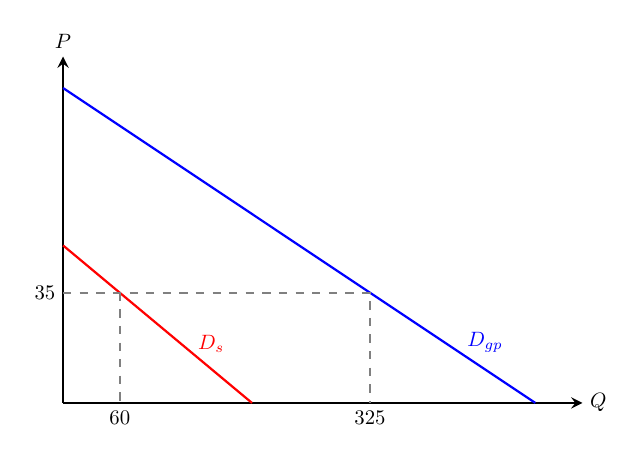
\begin{tikzpicture}[x=0.012cm, y=0.04cm, >=stealth, thick, every node/.style={scale=0.75}]
				\draw[->] (0,0) -- (550,0) node[right] {$Q$};
				\draw[->] (0,0) -- (0,110) node[above] {$P$};
				
				% 大众需求 P = 100 - 0.2Q
				\draw[blue] (0,100) -- (500,0) node[pos=0.85, above right, fill=white, inner sep=1pt] {$D_{gp}$};
				% 学生需求 P = 50 - 0.25Q
				\draw[red] (0,50) -- (200,0) node[pos=0.7, above right, fill=white, inner sep=1pt] {$D_s$};
				
				\draw[dashed, gray] (0,35) node[left, black] {$35$} -- (325,35) -- (325,0) node[below, black] {$325$};
				\draw[dashed, gray] (60,35) -- (60,0) node[below, black] {$60$};
			\end{tikzpicture}
		\end{center}
		
		b. 需求价格弹性计算
		
		根据需求点弹性的定义公式：
		$$ E_d = \frac{dQ}{dP} \cdot \frac{P}{Q} $$
		
		对于普通大众群体，在 $P=35$ 时的弹性为：
		$$ E_{d,gp} = (-5) \times \frac{35}{325} \approx -0.54 $$
		由于 $|E_{d,gp}| < 1$，说明该群体需求缺乏弹性。
		
		对于学生群体，在 $P=35$ 时的弹性为：
		$$ E_{d,s} = (-4) \times \frac{35}{60} \approx -2.33 $$
		由于 $|E_{d,s}| > 1$，说明该群体需求富有弹性。
		
		c. 收益最大化判定
		
		根据总收益与需求弹性的关系：
		$$ \frac{dTR}{dP} = Q(1 + E_d) $$
		当 $|E_d| < 1$ 时，价格与总收益同向变动，提价能增加收益；当 $|E_d| > 1$ 时，价格与总收益反向变动，降价能增加收益。
		目前普通大众缺乏弹性，应通过涨价增加收益；而学生群体富有弹性，应通过降价增加收益。因此，统一标价 35 美元并未实现总收益最大化。
		
		d. 总收益最大化定价
		
		方法一：边际收益法
		
		总收益最大化的必要条件是边际收益等于零，即：
		$$ MR = \frac{dTR}{dQ} = 0 $$
		
		对于普通大众，反需求函数为 $P = 100 - 0.2Q$，则：
		$$ TR_{gp} = 100Q - 0.2Q^2 $$
		$$ MR_{gp} = 100 - 0.4Q = 0 \implies Q^* = 250 $$
		代入需求函数得最优价格：
		$$ P_{gp}^* = 100 - 0.2 \times 250 = 50 $$
		
		对于学生群体，反需求函数为 $P = 50 - 0.25Q$，则：
		$$ TR_s = 50Q - 0.25Q^2 $$
		$$ MR_s = 50 - 0.5Q = 0 \implies Q^* = 100 $$
		代入需求函数得最优价格：
		$$ P_s^* = 50 - 0.25\times 100 = 25 $$
		
		方法二：二次函数最值法
		
		直接建立总收益关于价格 $P$ 的二次函数：
		$$ TR(P) = P \cdot Q(P) $$
		
		对于普通大众：
		$$ TR_{gp} = P(500 - 5P) = -5P^2 + 500P $$
		根据二次函数 $y = ax^2 + bx + c$ 的顶点公式 $x = -b/2a$，总收益最大化的价格为：
		$$ P_{gp}^* = \frac{-500}{2 \times (-5)} = 50 $$
		
		对于学生群体：
		$$ TR_s = P(200 - 4P) = -4P^2 + 200P $$
		总收益最大化的价格为：
		$$ P_s^* = \frac{-200}{2 \times (-4)} = 25 $$
		
		\begin{center}
			\begin{tikzpicture}[>=stealth, thick, every node/.style={scale=0.75}]
				% === 左图：普通大众 ===
				\begin{scope}[x=0.012cm, y=0.04cm]
					\draw[->] (0,0) -- (550,0) node[right] {$Q$};
					\draw[->] (0,0) -- (0,110) node[above] {$P, MR$};
					
					% 需求曲线与MR曲线
					\draw[blue] (0,100) -- (500,0) node[pos=0.9, above right] {$D_{gp}$};
					\draw[blue, dashed] (0,100) -- (250,0) node[below] {$100$};
					
					% 收益最大化点
					\draw[dashed, gray] (250,0) -- (250,50) -- (0,50) node[left, black] {$50$};
					\fill (250,50) circle (2pt) node[above right, fill=white, inner sep=1pt] {$E_1$};
					
					\node[below] at (250,-15) {(1) 普通大众 (最优 $P=50$)};
				\end{scope}
				
				% === 右图：学生群体 ===
				\begin{scope}[xshift=7.5cm, x=0.025cm, y=0.07cm]
					\draw[->] (0,0) -- (220,0) node[right] {$Q$};
					\draw[->] (0,0) -- (0,60) node[above] {$P, MR$};
					
					% 需求曲线与MR曲线
					\draw[red] (0,50) -- (200,0) node[pos=0.8, above right] {$D_s$};
					\draw[red, dashed] (0,50) -- (100,0) node[below] {$100$};
					
					% 收益最大化点
					\draw[dashed, gray] (100,0) -- (100,25) -- (0,25) node[left, black] {$25$};
					\fill (100,25) circle (2pt) node[above right, fill=white, inner sep=1pt] {$E_2$};
					
					\node[below] at (100,-8) {(2) 学生群体 (最优 $P=25$)};
				\end{scope}
			\end{tikzpicture}
		\end{center}
		
		
		\item \textbf{朱蒂已经决定每年不多不少花 500 美元在大学教材上，尽管她知道价格每年可能要上涨，并且她的祖父母明年将会给她一份可观的礼金。朱蒂对教材需求的价格弹性为多少？收入弹性呢？}
		
		\textbf{答：}
		1. 需求价格弹性分析：
		
		根据题意，朱蒂在教材上的总支出始终固定为 $P \cdot Q = 500$ 美元。由此可推导出她的教材需求函数为：
		$$Q = 500P^{-1}$$
		对该需求函数关于价格 $P$ 求导，得：
		$$\frac{dQ}{dP} = -500P^{-2}$$
		将其代入需求价格弹性公式 $E_d = \frac{dQ}{dP} \cdot \frac{P}{Q}$：
		$$E_d = \left( -500P^{-2} \right) \cdot \frac{P}{500/P} = -1$$
		朱蒂对教材的需求价格弹性恒等于 $-1$，属于单位弹性（Unit Elastic）。这意味着价格变动产生的支出效应完全被需求量的反向变动所抵消，总支出保持不变。
		
		2. 需求收入弹性分析：
		
		需求收入弹性定义为需求量变动百分比与收入变动百分比的比值。根据朱蒂的决策规则，无论其总收入 $I$（包括祖父母提供的礼金）如何变化，她分配给教材的预算始终固定为 500 美元。
		由于需求函数 $Q = 500/P$ 中不包含收入变量 $I$，即：
		$$\frac{\partial Q}{\partial I} = 0$$
		因此，需求收入弹性为：
		$$E_I = \frac{\partial Q}{\partial I} \cdot \frac{I}{Q} = 0$$
		朱蒂对教材的需求收入弹性为 $0$，说明教材在她的预算决策中表现为收入无弹性的商品。
		
		\begin{center}
			\begin{tikzpicture}[scale=0.6, >=stealth, thick, every node/.style={scale=0.8}, x=0.1cm, y=0.1cm]
				% 坐标轴
				\draw[->] (0,0) -- (65,0) node[right] {$Q$};
				\draw[->] (0,0) -- (0,65) node[above] {$P$};
				
				% 需求曲线 (PQ=500 -> P=500/Q)
				\draw[domain=8:58, samples=100, color=blue, very thick] plot (\x, {500/\x});
				\node[blue, right] at (58, 8.6) {$PQ=500$};
				
				% 选取两个点展示 TR 不变
				\draw[dashed, gray] (10,0) node[below, black] {$10$} -- (10,50) -- (0,50) node[left, black] {$50$};
				\draw[dashed, gray] (25,0) node[below, black] {$25$} -- (25,20) -- (0,20) node[left, black] {$20$};
				
				\fill (10,50) circle (2pt);
				\fill (25,20) circle (2pt);
				
				% 标注面积相等 (TR1 = TR2)
				\node[fill=white, inner sep=1pt] at (30,40) {\footnotesize $E_d = -1$};
			\end{tikzpicture}
		\end{center}
	
	\newpage
	\item \textbf{ACME公司确定，在目前的价格上，其计算机芯片的短期需求价格弹性为－2，其磁盘驱动器的短期需求价格弹性为－1。\\
		a. 如果公司决定将两种产品的价格都提高10％，其销售量会有什么变化？销售收入呢？\\
		b. 你能否从已知的信息中判断，哪个产品会给厂商带来最大的收入？如果能，为什么？如果不能，你还需要什么别的信息？}
	
	\textbf{答：}
	根据需求价格弹性定义及销售收入公式（$TR = P \times Q$），其核心计算关系如下：
	$$ \frac{\Delta Q}{Q} = E_d \times \frac{\Delta P}{P} $$
	$$ \frac{\Delta TR}{TR} = \left(1 + \frac{\Delta P}{P}\right)\left(1 + \frac{\Delta Q}{Q}\right) - 1 $$
	
	a. 当价格均提高10\%

		计算机芯片（$E_d = -2$）：
		$$ \frac{\Delta Q}{Q} = -2 \times 10\% = -20\% $$
		$$ \frac{\Delta TR}{TR} = (1+10\%)(1-20\%) - 1 = -12\% $$
		销量下降 20\%，销售收入下降 12\%。
		
		磁盘驱动器（$E_d = -1$）：
		$$ \frac{\Delta Q}{Q} = -1 \times 10\% = -10\% $$
		$$ \frac{\Delta TR}{TR} = (1+10\%)(1-10\%) - 1 = -1\% $$
		销量下降 10\%，销售收入下降 1\%。
	
	b. 不能判断。弹性信息仅反映价格变动对收入的边际影响（变动率），无法决定总收入的绝对水平。要比较两者总收入，还需获知两种产品的初始价格 $P$ 与初始销量 $Q$。
	
	\begin{center}
		\begin{tikzpicture}[scale=0.75, >=stealth, thick, every node/.style={scale=0.85}]
			% 坐标轴
			\draw[->] (0,0) -- (6.5,0) node[right] {$Q$};
			\draw[->] (0,0) -- (0,5) node[above] {$P$};
			
			% 需求曲线
			\draw[blue] (1,4.5) -- (5.5,1) node[right] {$D$};
			
			% 弹性区域划分虚线
			\draw[dashed, gray] (3.25, 2.75) -- (3.25, 0) node[below, black] {中点};
			
			% 标注产品与弹性
			\fill (2.125, 3.625) circle (2pt) node[above right, fill=white, inner sep=1pt] {芯片 $|E_d|>1$};
			\fill (3.25, 2.75) circle (2pt) node[above right, fill=white, inner sep=1pt] {驱动器 $|E_d|=1$};

		\end{tikzpicture}
	\end{center}
	\newpage
	\item \textbf{观察在下面概述的情形中一个人的行为，然后确定每一种商品相关的需求收入弹性（即该商品是正常品还是劣等品）。如果你不能确定收入弹性，你还需要别的什么信息？\\
		a. 比尔将其全部收入花在书籍和咖啡上。当他在书店的一只旧纸箱子里翻找东西时发现了20美元，他马上去买了一本新的精装诗集。\\
		b. 比尔丢失了他打算用来购买一杯双份蒸馏咖啡的10美元，他决定把新书折价卖给他的朋友，再用换来的钱买咖啡。\\
		c. 像波希米亚人那样生活已成了最新时尚，结果，咖啡和书籍的价格上涨了25％。比尔将这两种商品的消费削减了同样的百分比。\\
		d. 比尔离开了艺术学校，而获得了一个工商管理硕士（MBA）学位。他不喝咖啡且不读书了。现在他读《华尔街日报》，喝瓶装的矿泉水。}
	
	\textbf{答：}
	需求收入弹性
	$$E_I = \frac{\Delta Q/Q}{\Delta I/I}$$
	若 $E_I > 0$ 为正常品；若 $E_I < 0$ 为劣等品。
	
	a.书籍是正常品，咖啡的收入弹性无法确定。\\捡到20美元（意外的正向收入冲击）使他立即增加了书籍的消费，说明书籍的收入弹性为正，没有看出他对咖啡消费的改变，所以无法判断咖啡。
	
	b.书籍是正常品，咖啡是劣等品或者说必需品。\\丢失10美元是实际购买力的净损失（负向收入冲击)。在比尔的收入下降时，会卖掉新书（对书的需求下降），说明书籍是正常品；而他不惜卖书也要维持咖啡的消费，说明咖啡在收入下降时其需求未减反增，甚至优先维持），属于劣等品或者说必需品。
	
	c. 无法确定两者的收入弹性。\\这是价格同比例变动引发的价格效应（包含替代效应与收入效应），在未明确比尔名义收入是否发生变动以及变动幅度的情况下，无法分离出纯粹的收入弹性。
	
	d.咖啡和书籍是劣等品，《华尔街日报》和瓶装矿泉水是正常品。\\获得MBA学位通常伴随着收入的显著提升。当比尔的收入增加后，咖啡和书籍的需求直接降低到0，这说明其收入弹性为负，而对报纸和矿泉水的需求的增加说明其收入弹性为正。
	
	\item \textbf{假设食品需求的收入弹性是0.5，价格弹性是－1.0。假设费利西亚每年在食品上花费10000美元，食品价格为2美元，她的收入为25000美元。\\
		a. 如果一项食品销售税使得食品价格上升至2.5美元，她的食品消费会有什么变化？（提示：涉及较大价格变化时应假设采用弧弹性）\\
		b. 假设费利西亚得到2500美元的退税以缓解该销售税的影响。她现在的食品消费又将如何呢？\\
		c. 当她得到的退税数额等于销售税的支付数额时，她的境况是改善了还是变糟了？请说明原因。}
	
	\textbf{答：}
	初始食品消费量为：$Q_1 = 10,000 / 2 = 5,000$ 单位。
	
	a. 采用弧弹性公式计算价格上升后的消费量 $Q_2$：
	\[
	\begin{aligned}
		E_d &= \frac{\Delta Q / \bar{Q}}{\Delta P / \bar{P}} = \frac{Q_2 - 5000}{(5000 + Q_2)/2} / \frac{2.5 - 2.0}{(2.0 + 2.5)/2}
	\end{aligned}
	\]
	解得 $Q_2 = 4,000$ 单位。即食品消费量减少了 1,000 单位。
	
	b. 得到 2,500 美元退税后，收入变动率为 $\Delta I / I = 2,500 / 25,000 = 10\%$。
	根据需求收入弹性公式：
	\[
	\frac{\Delta Q}{Q} = E_I \cdot \frac{\Delta I}{I} = 0.5 \times 10\% = 5\%
	\]
	以 $Q_2$ 为基数计算，新的消费量为：$Q_3 = 4,000(1 + 5\%) = 4,200$ 单位。
	
	c. 费利西亚的境况变糟了。
	虽然退税能够在一定程度上弥补购买力的损失，但是销售税改变了食品和其他商品的相对价格，即使退税额等于其支付的税款，由于替代效应，消费者仍会减少对受税商品的消费并调整最优消费组合。根据显示偏好原理，退税后的新预算线虽经过或接近原来的点，但斜率已变化，消费者的最优选择点必然在无差异曲线下方区域。
	
	\begin{center}
		\begin{tikzpicture}[x=0.6cm, y=0.6cm, >=stealth, every node/.style={scale=0.8}]
			% 1. 坐标轴
			\draw[->, thick] (0,0) -- (15,0) node[right] {食品 $X$};
			\draw[->, thick] (0,0) -- (0,11) node[above] {其他商品 $Y$};
			
			% 2. 预算线逻辑计算 (采用夸大的退税截距以彻底分离曲线)：
			% L1 (初始): y = 8 - 4/7x 
			% L2 (征税): y = 8 - 1.25x (绕纵轴截距旋转，变得陡峭)
			% L3 (退税): y = 10 - 1.25x (平行外移，截距夸大至10以实现视觉分离)
			\draw[thick, black] (0,8) -- (14,0) node[pos=0.85, above right, inner sep=1pt] {$L_1$};
			\draw[thin, dashed, gray] (0,8) -- (6.4,0) node[pos=0.8, below left, inner sep=1pt] {$L_2$};
			\draw[thick, gray] (0,10) -- (8,0) node[pos=0.85, above left, inner sep=1pt, xshift=-4pt] {$L_3$};
			
			% 3. 无差异曲线绘制 (严格计算的一阶导数相切点坐标):
			% U0 (初始均衡): 与 L1 精确相切于 E0(7, 4), 系数 k = 28
			\draw[thick, blue, domain=2.8:13, samples=100] plot (\x, {28/\x}) node[right] {$U_0$};
			
			% U1 (最终均衡): 与 L3 精确相切于 E1(4, 5), 系数 k = 20
			\draw[thick, red, domain=2.0:9.5, samples=100] plot (\x, {20/\x}) node[right] {$U_1$};
			
			% 4. 均衡点标注 
			\filldraw[fill=white, draw=black, thick] (7,4) circle (1.5pt) node[above right, inner sep=2pt] {$E_0$};
			\filldraw[fill=white, draw=black, thick] (4,5) circle (1.5pt) node[above left, inner sep=2pt,yshift=-6pt,xshift=-3pt] {$E_1$};
			
			% 5. 辅助投影线与刻度标注
			\draw[dashed, gray] (7,0) node[below, black] {$5000$} -- (7,4);
			\draw[dashed, gray] (4,0) node[below, black, xshift=-4pt] {$4200$} -- (4,5);
			
		\end{tikzpicture}
	\end{center}
	
	\item \textbf{假设你经营着一个小企业，想预测你的产品价格提高之后需求量会发生什么变化。虽然你不知道你的产品的确切需求曲线，但是你知道第一年你要价45美元，销售了1200单位，第二年你要价30美元，销售了1800单位。\\
		a. 如果你打算把价格提高10％，那么，以百分比的形式计，对需求量变动的一个合理预测为多少？\\
		b. 如果你把价格提高10％，收入将会上升还是下降？}
	
	\textbf{答：}
	a. 首先运用弧弹性公式估算该区间的需求价格弹性：
	$$E_d = \frac{\Delta Q}{(Q_1+Q_2)/2} / \frac{\Delta P}{(P_1+P_2)/2} = -1$$
	由于价格提高 10\%，合理预测的需求量变动率为
	$$\frac{\Delta Q}{Q} = E_d \times 10\% = -10\%$$
	需求量将减少 10\%。
	
	b. 销售收入基本不变。由于该区间的需求弹性为单位弹性（$|E_d| = 1$），价格上升带来的正向边际收入与销量下降带来的负向边际损失刚好相互抵消。
	
	现价30美元，销量1800，初始收入 $TR = 54000$。提价10\%至33美元，销量下降10\%至1620，新收入 $TR = 33 \times 1620 = 53460$，两者差距极小。
	
	\newpage
	\item \textbf{假设你在管理一座营运成本基本上为零的收费桥梁。过桥需求 $Q$ 由 $P=15-(1/2)Q$ 给出。\\
		a. 画出过桥服务的需求曲线。\\
		b. 如果不收费，会有多少人通过该桥？\\
		c. 如果过桥费是5美元，相对应的消费者剩余的损失是多少？\\
		d. 该收费桥梁的运营方打算把价格提高到7美元。在这一相对较高的价格上，会有多少人通过该桥？该收费桥梁的收益是上升还是下降了？从你的答案出发，你对需求弹性有何判断？\\
		e. 求与价格从5美元上升到7美元相对应的消费者剩余的损失。}
	
	\textbf{答：}
	a. 需求曲线 $P = 15 - 0.5Q$ 是一条向下倾斜的直线，其纵轴截距为 15，横轴截距为 30,如下图所示）。
	
	b. 当不收费时（$P = 0$）：
	\[ 0 = 15 - 0.5Q \implies Q = 30 \]
	即会有 30 人通过该桥。
	
	c. 消费者剩余损失为两次价格水平下 $CS$ 的差值：
	\[ CS_0 (P=0) = \frac{1}{2} \times 30 \times 15 = 225 \]
	\[ CS_1 (P=5) = \frac{1}{2} \times 20 \times (15-5) = 100 \]
	\[ \Delta CS = 225 - 100 = 125 \text{ 美元} \]
	
	d. 当价格提高到 $P = 7$ 时，过桥人数 $Q = 2 \times (15 - 7) = 16$。
	收益变动分析如下：
	\[ TR_1 = 5 \times 20 = 100, \quad TR_2 = 7 \times 16 = 112 \]
	由于 $TR_2 > TR_1$，总收益上升。
	这表明在 $P \in [5, 7]$ 区间内，需求价格弹性 $|E_d| < 1$，即需求是缺乏弹性的，价格上涨带来的单位收益增加超过了销量下降的损失。
	
	e. 价格从 5 美元上升到 7 美元对应的消费者剩余损失为：
	\[ CS_2 (P=7) = \frac{1}{2} \times 16 \times (15-7) = 64 \]
	\[ \text{损失} = CS_1 - CS_2 = 100 - 64 = 36 \text{ 美元} \]
	
	\begin{center}
		\begin{tikzpicture}[scale=0.7, >=stealth, thick, every node/.style={scale=0.85}]
			% --- 左图：P=0 到 P=5 的变动 ---
			\begin{scope}[xshift=0cm]
				\draw[->] (0,0) -- (6.5,0) node[right] {$Q$};
				\draw[->] (0,0) -- (0,5.5) node[above] {$P$};
				
				% 需求曲线 (x=Q/5, y=P/3)
				\draw[blue] (0,5) node[left, black] {15} -- (6,0) node[below, black] {30};
				
				% P=5 辅助线
				\draw[dashed, gray] (0,1.67) node[left, black] {5} -- (4,1.67) -- (4,0) node[below, black] {20};
				
				% CS损失区域 (梯形 0,0, 4,1.67, 6,0)
				\fill[red, fill opacity=0.2] (0,0) -- (0,1.67) -- (4,1.67) -- (6,0) -- cycle;
				\node[red!80!black, fill=white, inner sep=1pt] at (2,0.8) {$\Delta CS = 125$};
				\node[below] at (3,-0.8) {(1) $P=0 \to 5$ 时的福利损失};
			\end{scope}
			
			% --- 右图：P=5 到 P=7 的变动 ---
			\begin{scope}[xshift=8.5cm]
				\draw[->] (0,0) -- (6.5,0) node[right] {$Q$};
				\draw[->] (0,0) -- (0,5.5) node[above] {$P$};
				
				\draw[blue] (0,5) node[left, black] {15} -- (6,0) node[below, black] {30};
				
				% P=5 辅助线
				\draw[dashed, gray] (0,1.67) node[left, black, xshift=-2pt] {5} -- (4,1.67) -- (4,0) node[below, black] {20};
				% P=7 辅助线
				\draw[dashed, gray] (0,2.33) node[left, black, xshift=-2pt] {7} -- (3.2,2.33) -- (3.2,0) node[below, black] {16};
				
				% CS损失区域 (梯形 0,1.67, 0,2.33, 3.2,2.33, 4,1.67)
				\fill[orange, fill opacity=0.3] (0,1.67) -- (0,2.33) -- (3.2,2.33) -- (4,1.67) -- cycle;
				\node[orange!80!black, fill=white, inner sep=1pt] at (1.6,2) {损失 $= 36$};
				\node[below] at (3,-0.8) {(2) $P=5 \to 7$ 时的福利损失};
			\end{scope}
		\end{tikzpicture}
	\end{center}
	
	\newpage
	\item \textbf{维拉正打算升级她那台新的个人计算机上的操作系统。她听说新操作系统Linux在技术上优于Windows而且价格低很多。然而，在询问了她的朋友之后，她发现他们用的都是装了Windows的个人计算机。他们也认为Linux的拷贝相对较少。维拉选择了Windows。你能解释一下她的决定吗？}
	
	\textbf{答：}
	维拉的决定是正网络外部性（连带外部效应或攀比效应）的典型体现。一个消费者如果需求随着其他人购买该商品数量增加而相应地增多时，那么就存在正的网络外部性。尽管Linux具有技术和价格上的内生优势，但操作系统核心效用更依赖于市场的大规模用户基数，由于维拉的朋友及广大市场都在广泛使用Windows，这种庞大的网络不仅提供了直接的文件兼容、社交等便利，还构筑起远超Linux丰富应用软件和硬件支持；反之则必须独自面对极高的学习成本以及软件缺失造成的隐形折损。因此，Windows巨大的正向网络外部性收益远远超出了Linux价格和技术上的优势，这也是维拉做出最终决策的根本原因。
	
	\item \textbf{假设你是一个农业合作组织的顾问，该组织正在决定其成员明年要不要将他们的棉花生产减半。该组织需要你的建议，即这个决定是否将会提高其成员的收益。了解到棉花（$C$）与大豆（$S$）的种植面积在南方是竞争性的，你对棉花需求的估计为 $C=3.5-1.0P_C+0.25P_S+0.50I$，这里 $P_C$ 为棉花的价格，$P_S$ 为大豆的价格，$I$ 为收入。你是该支持还是反对这项计划？是否需要更多的信息以使你能够做出确切的回答？}
	
	\textbf{答：}
	不能直接得出支持或反对的结论，需要更多的核心市场信息。判定减产能否提高总收益，其核心在于评估棉花的需求价格弹性。如果棉花需求缺乏弹性，即 $|E_d| < 1$，则减产导致的价格涨幅将超过产量的跌幅，从而增加总收益；反之，若需求富有弹性，减产会使总收益锐减。
	
	给定的需求函数仅仅提供了需求曲线的斜率系数 
	$$\frac{\partial C}{\partial P_C} = -1.0$$
	根据点弹性公式：
	$$ E_d = \frac{\partial C}{\partial P_C} \cdot \frac{P_C}{C} = -1.0 \times \frac{P_C}{C} $$
	要计算具体的弹性值并做出确切回答，我们必须另外获得以下信息：一是当期大豆的市场价格$P_S$和宏观收入水平$I$，这用来测算基期棉花实际需求量$C$和市场均衡价格$P_C$；二是其他独立棉花产区供给反应预期。如果其它独立棉花产区不减产甚至增加产量填补空缺，合作社单边减产也没有办法推高市场价格$P_C$，最终只会失去市场份额、导致损失利润。
	
	\newpage
	\item \textbf{一个消费者只吃牛排和土豆。其预算为每10天30美元，而她必须买足够的土豆来吃，至少每天2单位。\\
		a. 土豆价格为0.5美元，牛排价格为10美元。消费者将消费两种商品各多少？\\
		b. 现在假设土豆的价格上升为1美元。消费者购买每种商品各多少？\\
		c. 现在假设土豆价格上升为1.25美元。消费者购买每种商品各多少？\\
		d. 土豆是哪种商品？\\
		e. 你预测土豆的需求曲线会一直保持这种趋势吗？为什么？}
	
	\textbf{答：}
	设消费的土豆数量为 $X$，牛排数量为 $Y$。消费者的预算约束为 $P_X X + P_Y Y = 30$。维持生存的极值约束为 $X \ge 20$（即 10 天至少消费 20 单位土豆）。
	
	a. 当 $P_X = 0.5, P_Y = 10$ 时。
	维持生存至少需购买 20 单位土豆，花费 $20 \times 0.5 = 10$ 美元。剩余 20 美元预算恰好可购买 2 单位牛排。因此，消费组合为 20 单位土豆，2 单位牛排。
	
	b. 当 $P_X = 1$ 时。
	维持生存至少需购买 20 单位土豆，花费 $20 \times 1 = 20$ 美元。剩余 10 美元预算恰好可购买 1 单位牛排。因此，消费组合为 20 单位土豆，1 单位牛排。
	
	c. 当 $P_X = 1.25$ 时。
	维持生存的 20 单位土豆需花费 $20 \times 1.25 = 25$ 美元。剩余 5 美元不足以购买 1 单位的完整牛排。由于牛排不可细分，为了满足生存需要并耗尽预算，所有的资金将被迫全部投入土豆的购买中：
	$$ X = \frac{30}{1.25} = 24 $$
	因此，消费组合为 24 单位土豆，0 单位牛排。
	
	d. 土豆是吉芬品。当土豆价格从 1 美元升至 1.25 美元时，预算空间的极度压缩产生了巨大的负向收入效应。由于必须满足绝对的生存线限制，消费者被迫放弃了昂贵的肉类，转而增加了对廉价主食（土豆）的需求量（从 20 增至 24）。这表现出了“价格上升，需求量反而增加”的违背需求法则的典型特征。
	
	e. 不会一直保持这种趋势。一旦土豆价格超过 1.5 美元（此时 30 美元的总预算全部用于买土豆也无法达到 20 单位的最低生存线），预算约束将彻底崩塌。为了生存，消费者将被迫放弃现有的消费组合体系，去寻找更廉价的替代主食，此时土豆的需求量必然急剧下降。
	
	\begin{center}
		\begin{tikzpicture}[x=0.3cm, y=1.2cm, >=stealth, thick, every node/.style={scale=0.85}]
			% 1. 坐标轴
			\draw[->] (0,0) -- (32,0) node[right] {土豆 $X$};
			\draw[->] (0,0) -- (0,3.6) node[above] {牛排 $Y$};
			
			% 纵轴截距
			\node[left] at (0,3) {$3$};
			
			% 2. 最低消费生存线 (移到底层，颜色调淡，避免喧宾夺主)
			\draw[dashed, red!50, very thick] (20,0) -- (20,3.3) 
			node[above, red!80!black] {$X \ge 20$};
			
			% 3. 预算线演变 (错开标签位置，彻底消除重叠)
			% 预算线 1 (P_x = 0.5) - 浅灰，标签放末端
			\draw[gray] (0,3) -- (28, 1.6) node[right] {$P_X=0.5$};
			
			% 预算线 2 (P_x = 1.0) - 深灰，标签放末端
			\draw[darkgray] (0,3) -- (30, 0) node[above right] {$P_X=1.0$};
			
			% 预算线 3 (P_x = 1.25) - 主题蓝，标签放线段中下部开阔处
			\draw[blue] (0,3) -- (24, 0);
			\node[blue, below left,yshift=3pt] at (14, 1.25) {$P_X=1.25$};
			
			% 4. 投影虚线 (细化线条，精简文字)
			\draw[dashed, gray, thin] (0,2) node[left, black] {$2$} -- (20,2);
			\draw[dashed, gray, thin] (0,1) node[left, black] {$1$} -- (20,1);
			
			% X轴关键刻度
			\draw (20,0) -- (20,-0.1) node[below] {$20$};
			\draw (24,0) -- (24,-0.1) node[below] {$24$};
			
			% 5. 均衡点 (仅保留代号，坐标已由坐标轴自然体现)
			\fill[gray] (20,2) circle (2pt) node[above right] {$E_1$};
			\fill[darkgray] (20,1) circle (2pt) node[above right] {$E_2$};
			\fill[blue] (24,0) circle (2pt) node[above right] {$E_3$};
			
			% 6. 吉芬效应指示 (移至横轴下方，彻底解决画面内部拥挤)
			\draw[->, red, thick] (20.5, -0.5) -- (23.5, -0.5) node[midway, below] {吉芬效应};
		\end{tikzpicture}
	\end{center}
	
	\end{enumerate}
	
	\newpage
	\section{附录练习题}
	\begin{enumerate}[label=\textbf{\arabic*.}, leftmargin=*]
		\item \textbf{下面的效用函数中哪些符合凸的无差异曲线？哪些并不符合？}\\
			a. \( U(X,Y) = 2X + 5Y \)\\
			b. \( U(X,Y) = (XY)^{0.5} \)\\
			c. \( U(X,Y) = \min(X,Y) \)，这里 $\min$ 为 $X$ 和 $Y$ 两个数值中的最小值。\\
			d. \( U(X,Y) = \log(X) + \log(Y) \)
		
		\textbf{答：}
		无差异曲线凸性的定义：偏好是凸的，当且仅当任意两个无差异消费束的加权平均至少与原消费束一样好。其中，边际替代率（$MRS$）严格递减对应严格凸，$MRS$ 非递增对应弱凸。
		
		\begin{enumerate}[label=\textbf{\alph*.}, leftmargin=2em]
			\item $U(X,Y) = 2X + 5Y$：完全替代型效用函数，无差异曲线为直线，$MRS=MU_X/MU_Y=0.4$（恒定不变），属于弱凸。
			\item $U(X,Y) = (XY)^{0.5}$：柯布-道格拉斯效用函数，$MRS=Y/X$（随 $X$ 增加严格递减），无差异曲线凸向原点，属于严格凸。
			\item $U(X,Y) = \min(X,Y)$：完全互补型效用函数，无差异曲线为 L 形，两种商品必须按固定比例消费，不存在替代关系，属于弱凸。
			\item $U(X,Y) = \log(X) + \log(Y) = \log(XY)$：这是柯布-道格拉斯效用函数的严格单调递增变换，与 (b) 代表完全相同的偏好，$MRS=Y/X$ 严格递减，无差异曲线同样凸向原点，属于严格凸。
		\end{enumerate}
		
		\begin{center}
			\begin{tikzpicture}[scale=0.75, >=stealth, thick, every node/.style={scale=0.85}]
				% 完全替代 (a)
				\begin{scope}[xshift=0cm]
					\draw[->] (0,0) -- (4,0) node[right] {$X$};
					\draw[->] (0,0) -- (0,4) node[above] {$Y$};
					\draw[blue] (0.5, 3.0) -- (3.5, 1.2) node[right, fill=white, inner sep=1pt] {$U$};
					\node[below] at (2,-0.5) {(a) 弱凸 (直线)};
				\end{scope}
				% 柯布-道格拉斯 (b)(d)
				\begin{scope}[xshift=5.8cm]
					\draw[->] (0,0) -- (4,0) node[right] {$X$};
					\draw[->] (0,0) -- (0,4) node[above] {$Y$};
					\draw[red, domain=0.6:3.5, samples=100] plot (\x, {2.1/\x}) node[right, fill=white, inner sep=1pt] {$U$};
					\node[below] at (2,-0.5) {(b)(d) 严格凸 (双曲线)};
				\end{scope}
				% 完全互补 (c)
				\begin{scope}[xshift=11.6cm]
					\draw[->] (0,0) -- (4,0) node[right] {$X$};
					\draw[->] (0,0) -- (0,4) node[above] {$Y$};
					\draw[green!60!black] (1.8, 3.5) -- (1.8, 1.8) -- (3.5, 1.8) node[right, fill=white, inner sep=1pt] {$U$};
					\draw[dashed, gray] (0,0) -- (1.8, 1.8);
					\node[below] at (2,-0.5) {(c) 弱凸 (L形)};
				\end{scope}
			\end{tikzpicture}
		\end{center}
		
		\item \textbf{说明下面两个效用函数所导出的商品 $X$ 和 $Y$ 的需求函数相同。\\
			a. \( U(X,Y) = \log(X) + \log(Y) \)\\
			b. \( U(X,Y) = (XY)^{0.5} \)}
		
		\textbf{答：}
		正单调变换不改变消费者的序数偏好，因此得出的最优消费选择与需求函数完全一致。设商品价格为 $P_X, P_Y$，收入为 $I$，预算约束为 $P_X X + P_Y Y = I$。
		
		\textbf{a. $U(X,Y) = \log(X) + \log(Y) = \log(XY)$}
		
		消费者效用最大化的一阶条件为边际效用之比等于价格之比：
		$$\frac{MU_X}{MU_Y} = \frac{Y}{X} = \frac{P_X}{P_Y} \implies Y = \frac{P_X}{P_Y}X$$
		代入预算约束方程：
		$$P_X X + P_Y \left( \frac{P_X}{P_Y}X \right) = I \implies 2P_X X = I$$
		解得需求函数为：
		$$X^* = \frac{I}{2P_X}, \quad Y^* = \frac{I}{2P_Y}$$
		
		\textbf{b. $U(X,Y) = (XY)^{0.5}$}
		
		同样根据一阶条件求解：
		$$\frac{MU_X}{MU_Y} = \frac{0.5X^{-0.5}Y^{0.5}}{0.5X^{0.5}Y^{-0.5}} = \frac{Y}{X} = \frac{P_X}{P_Y} \implies Y = \frac{P_X}{P_Y}X$$
		由于边际替代率与 (a) 完全相同，代入预算约束后得到的需求函数也完全一致：
		$$X^* = \frac{I}{2P_X}, \quad Y^* = \frac{I}{2P_Y}$$
		
		\item \textbf{假设效用函数由 $U(X,Y) = \min(X,Y)$ 给出，正如练习题1中的c部分所示。那么将因为 $X$ 价格的变化而引起的其需求的变化进行分解的斯卢茨基方程是什么？什么是收入效应？什么是替代效应？}
		
		\textbf{答：}
		对于完全互补品 $U(X,Y) = \min(X,Y)$，消费者的最优选择始终满足固定比例消费，即 $X = Y$。结合预算约束方程 $P_X X + P_Y Y = I$，可推导出该商品的初始需求函数为：
		$$X = \frac{I}{P_X + P_Y}$$
		
		斯卢茨基方程的一般形式将价格变动引起的总效应精确分解为替代效应和收入效应两部分：
		$$ \underbrace{\frac{\partial X}{\partial P_X}}_{\text{总效应}} = \underbrace{\left. \frac{\partial X}{\partial P_X} \right|_{\bar{U}}}_{\text{替代效应}} + \underbrace{\left( -X \frac{\partial X}{\partial I} \right)}_{\text{收入效应}} $$
		
		针对完全互补品：
		
		替代效应：由于商品必须按固定比例消费，无差异曲线呈现为直角 L 型。当相对价格发生变化时，如果对消费者进行收入补偿以维持其原有效用水平，其最优消费组合依然被死死锁定在无差异曲线的直角拐点上，不存在两种商品之间的相互替代。因此，完全互补品的替代效应恒等于 $0$，即
		$$\left. \frac{\partial X}{\partial P_X} \right|_{\bar{U}} = 0$$
		
		收入效应：既然替代效应为零，价格的变化便仅仅通过改变消费者的实际购买力来影响需求。当 $X$ 的价格发生变化时，引起的实际收入变动带来的收入效应计算如下：
		$$ -X \frac{\partial X}{\partial I} = -X \left( \frac{1}{P_X + P_Y} \right) = - \frac{I}{(P_X + P_Y)^2} $$
		
		总效应：价格变化带来的总效应完全由收入效应构成。对需求函数直接求导也可印证此结论：
		$$ \frac{\partial X}{\partial P_X} = - \frac{I}{(P_X + P_Y)^2} $$
		
		这说明，对于完全互补品而言，其斯卢茨基方程退化并简化为总效应完全等于收入效应：
		$$ \frac{\partial X}{\partial P_X} = -X \frac{\partial X}{\partial I} $$
		
		\begin{center}
			\begin{tikzpicture}[x=0.8cm, y=0.8cm, >=stealth, thick, every node/.style={scale=0.85}]
				% 坐标轴
				\draw[->] (0,0) -- (9.5,0) node[right] {$X$};
				\draw[->] (0,0) -- (0,8.5) node[above] {$Y$};
				
				% 比例射线 X=Y
				\draw[dashed, gray] (0,0) -- (7.5,7.5);
				
				% 预算线 BL1
				\draw[black] (0,6) node[left] {$BL_1$} -- (9, 1.5) node[right] {$BL_1$}; 
				
				% 预算线 BL2 (X价格上升)
				\draw[blue] (0,6) -- (6,0) node[below] {$BL_2$};
				
				% 斯卢茨基补偿预算线 BLC (经过 E1，平行于 BL2)
				\draw[red, dashed] (0,8) node[left] {$BL_C$} -- (8,0) node[below] {$BL_C$};
				
				% L型无差异曲线
				\draw[thick, blue] (3,6.5) -- (3,3) -- (6.5,3) node[right] {$U_2$};
				\draw[thick, blue] (4,7.5) -- (4,4) -- (7.5,4) node[right] {$U_1$};
				
				% 均衡点 (使用 fill=white 防止遮挡网格与连线)
				\fill[black] (4,4) circle (2pt) node[above right, fill=white, inner sep=1pt,yshift=2pt,xshift=2pt] {$E_1 (E_C)$};
				\fill[black] (3,3) circle (2pt) node[below right, fill=white, inner sep=1pt,yshift=-3pt] {$E_2$};
				
				% 投影线与标注
				\draw[dashed, gray] (4,0) node[below, black] {$X_1$} -- (4,4);
				\draw[dashed, gray] (3,0) node[below, black] {$X_2$} -- (3,3);
				
				% 效应箭头
				\draw[->, purple, very thick] (3.8, -0.6) -- (3.2, -0.6) node[midway, below] {收入效应 = 总效应};
				\node[below, text=black] at (3.5, -1.3) {(替代效应 $= 0$)};
			\end{tikzpicture}
		\end{center}
		
		\item \textbf{莎伦的效用函数如下：$U(X,Y) = \sqrt{X} + \sqrt{Y}$。其中，$X$ 为她对单独包装的块状糖的消费量，价格 $P_X = 1$ 美元，$Y$ 为浓咖啡的消费量，价格 $P_Y = 3$ 美元。\\
			a. 推导莎伦对单独包装的块状糖和浓咖啡的需求函数。\\
			b. 假定她的收入 $I = 100$ 美元。莎伦将消费多少数量的单独包装的块状糖和浓咖啡？\\
			c. 收入的边际效用为多少？}
		
		\textbf{答：}
		
		\textbf{a. 推导需求函数}
		
		消费者预算约束为 $P_X X + P_Y Y = I$。分别计算商品的边际效用：
		$$MU_X = \frac{1}{2\sqrt{X}}, \quad MU_Y = \frac{1}{2\sqrt{Y}}$$
		根据效用最大化条件，边际效用之比等于价格之比：
		$$\frac{MU_X}{MU_Y} = \frac{\sqrt{Y}}{\sqrt{X}} = \frac{P_X}{P_Y} \implies \frac{Y}{X} = \left(\frac{P_X}{P_Y}\right)^2 \implies Y = \left(\frac{P_X}{P_Y}\right)^2 X$$
		代入预算约束方程中：
		$$P_X X + P_Y \left(\frac{P_X}{P_Y}\right)^2 X = I \implies X \left( P_X + \frac{P_X^2}{P_Y} \right) = I$$
		由此解得广义需求函数为：
		$$X^* = \frac{I}{P_X + P_X^2/P_Y}, \quad Y^* = \frac{I}{P_Y + P_Y^2/P_X}$$
		将已知的 $P_X = 1$ 和 $P_Y = 3$ 代入，得到具体的线性需求函数形式：
		$$X^* = \frac{I}{1 + 1/3} = \frac{3I}{4}, \quad Y^* = \frac{I}{3 + 9} = \frac{I}{12}$$
		
		\newpage
		\textbf{b. 计算具体消费量}
		
		将收入 $I = 100$ 美元代入推导出的需求函数中：
		$$X^* = \frac{3 \times 100}{4} = 75, \quad Y^* = \frac{100}{12} \approx 8.33$$
		即莎伦将消费 $75$ 块块状糖和约 $8.33$ 杯浓咖啡。
		
		\textbf{c. 计算收入的边际效用}
		
		收入的边际效用等于拉格朗日乘数 $\lambda$，根据一阶条件 
		$$\lambda = \frac{MU_X}{P_X}$$
		代入最优解进行计算：
		$$\lambda = \frac{1}{2P_X\sqrt{X^*}} \approx 0.0577$$
		这表明，在当前消费水平下，每增加 $1$ 美元的收入，莎伦的总效用将增加约 $0.0577$ 个单位。
		
		\item \textbf{莫里斯的效用函数如下：$U(X,Y) = 20X + 80Y - X^2 - 2Y^2$。其中，$X$ 为他对 CD 的消费量，价格为 1 美元，$Y$ 为他对录像带的消费量，租金价格为 2 美元。他计划在这两种形式的娱乐上花 41 美元。求最大化莫里斯效用的 CD 数量与录像带租赁数量。}
		
		\textbf{答：}
		根据题意，莫里斯的预算约束方程为 $X + 2Y = 41$。分别计算两种商品的边际效用：
		$$MU_X = 20 - 2X, \quad MU_Y = 80 - 4Y$$
		
		根据效用最大化条件，边际效用之比等于价格之比：
		$$\frac{MU_X}{MU_Y} = \frac{P_X}{P_Y} \implies \frac{20 - 2X}{80 - 4Y} = \frac{1}{2}$$
		化简得：$Y = X + 10$
		
		将 $Y = X + 10$ 联立代入预算约束方程：
		$$X + 2(X + 10) = 41 \implies X^* = 7$$
		$$Y^* = 7 + 10 = 17$$
		
		此时莫里斯的最大总效用为：
		$$U(7,17) = 20 \times 7 + 80 \times 17 - 7^2 - 2 \times 17^2) = 873$$
		
		\begin{center}
			\begin{tikzpicture}[x=0.4cm, y=0.2cm, >=stealth, thick, every node/.style={scale=0.85}]
				% 1. 坐标轴 (物理长宽比严格 1:1，呈现完美的方形包围盒)
				\draw[->] (0,0) -- (12,0) node[right] {$X$};
				\draw[->] (0,0) -- (0,24) node[above] {$Y$};
				\node[below left] at (0,0) {$O$};
				
				% 2. 预算线 BL: 只画到正方形边界 (X=11.5处)
				\draw[black] (0, 20.5) -- (11.5, 14.75);
				\fill[black] (0, 20.5) circle (1.5pt) node[left] {$20.5$};
				
				% 3. 无差异曲线 U=873
				\draw[blue!80, domain=4.9:11.5, samples=100, smooth] 
				plot (\x, {20 - sqrt(13.5 - 0.5*(\x-10)^2)}) 
				node[below right, font=\footnotesize] {$U=873$};
				
				% 4. 均衡点 E 与投影辅助线
				\coordinate (E) at (7, 17);
				\draw[dashed, gray!70, thin] (7,0) node[below, text=black] {$7$} -- (E) 
				-- (0,17) node[left, text=black] {$17$};
				\fill[red] (E) circle (1.5pt);
				
				% 5. 核心标签
				\node[above right, text=red, fill=white, inner sep=1pt, xshift=1pt, yshift=1pt] at (E) {$E(7,17)$};
			\end{tikzpicture}
		\end{center}
		
	\end{enumerate}
	% =======================================================
	%               第 5 章：不确定性与消费者行为
	% =======================================================
	\chapter{不确定性与消费者行为}
	
	\section{复习题}
	\begin{enumerate}[label=\textbf{\arabic*.}, leftmargin=*]
		\item \textbf{如果一个人是风险厌恶者，这意味着什么？为什么有些人厌恶风险，而有些人又喜好风险？}
		
		\textbf{答：}
		风险厌恶者是指在面临期望收益相同的确定性方案和不确定性方案时，总是偏好确定性结果。从效用函数来看，其效用函数具有严格凹性（边际效用递减），也就是说增加财富带来的边际效用减损小于减少财富所引起的效用变化。
		
		偏好差异的根源在于每个人的效用函数不同。风险厌恶者面对递减的边际效用。而风险喜好者却会拥有递增的边际效用（效用函数为凸）。这些差异由各种因素决定：一是极度贫困或极度富有都可能改变个体的风险边际偏好；二是心理感知，个人对损失的敏感程度（损失厌恶）不同；三是社会背景、职业特征等会造成不同的期望效用评估框架。
		
		\item \textbf{在对可变性的度量中，为什么方差比取值范围更好？}
		
		\textbf{答：}
		取值范围仅关注分布的两个极端点（最大值与最小值），完全忽略了所有中间结果及其发生的概率分布。若两个方案极值相同但其中一个结果更向均值集中，取值范围将无法区分其风险差异。
		
		方差通过计算所有可能结果与期望值偏离程度的平方，并以概率为权重进行加权平均，全面捕捉了概率分布的离散程度。它不仅考虑了变动的幅度，更考量了变动的频率，因此能够更科学、精准地衡量经济活动的风险（可变性）。
		\begin{center}
			\begin{tikzpicture}[x=0.6cm, y=1.2cm, >=stealth, thick, every node/.style={scale=0.85}]
				% 坐标轴
				\draw[->] (0,0) -- (10.5,0) node[right] {结果 ($X$)};
				\draw[->] (0,0) -- (0,3.6) node[above] {概率密度};
				
				% 绘制两条曲线 (使用 cos 函数的幂次来确保在 x=1 和 x=9 时完美收敛于 0)
				% 曲线A：方差小，集中 (8次幂使其陡峭)
				\draw[blue, thick, domain=1:9, samples=100] plot (\x, {3 * (cos((\x-5)*22.5))^8});
				
				% 曲线B：方差大，分散 (2次幂使其平缓)
				\draw[gray, thick, dashed, domain=1:9, samples=100] plot (\x, {1.4 * (cos((\x-5)*22.5))^2});
				
				% 均值辅助线
				\draw[dashed, thin, gray] (5,0) node[below, text=black] {$E[X]$} -- (5,3.2);
				
				% 边界辅助线 (极值点)
				\draw[dashed, thin, gray] (1,0) node[below, text=black] {$X_{\min}$} -- (1,0.6);
				\draw[dashed, thin, gray] (9,0) node[below, text=black] {$X_{\max}$} -- (9,0.6);
				
				% 标注曲线A (带白色背景防遮挡)
				\draw[->, thin, blue] (3.2, 2.8) node[above, fill=white, inner sep=1pt,xshift=-6pt] {方案 A: 方差小} to[bend left=15] (4.3, 2.1);
				
				% 标注曲线B (带白色背景防遮挡)
				\draw[->, thin, gray!90!black] (7.5, 1.8) node[above, fill=white, inner sep=1pt,xshift=5pt] {方案 B: 方差大} to[bend right=15] (6.6, 1.1);
				
				% 底部大括号表示“相同的取值范围”
				\draw[decorate, decoration={brace, amplitude=5pt, mirror}, black, thin] (1, -0.6) -- (9, -0.6) node[midway, below=5pt] {相同的取值范围};
			\end{tikzpicture}
		\end{center}
		\item \textbf{乔治有5000美元可以投资于共同基金。共同基金 A 的期望回报率为 15\%，共同基金 B 的期望回报率为 10\%。乔治应该选择共同基金 A 还是 B？}
		
		\textbf{答：}
		仅凭期望回报率无法进行理性决策。决策取决于乔治的风险偏好以及两只基金的风险水平（标准差）。
		
		若乔治为风险厌恶者，且基金 A 的风险显著高于基金 B，他可能会选择回报率较低但更稳健的基金 B。乔治的最优决策取决于他的无差异曲线与风险-收益预算线的切点。在未获得基金风险参数（标准差）和乔治风险系数的情况下，无法判定最终选择。
		
		\item \textbf{消费者追求期望效用最大化的含义是什么？你能举出某个人不追求期望效用最大化的例子吗？}
		
		\textbf{答：}
		期望效用最大化的核心含义是：消费者在不确定环境下做决策时，其目标不是追求“金钱数额”的平均值最大化，而是追求“金钱带来的满足感（效用）”的加权平均值最大化。
		由于边际效用递减，风险厌恶者会拒绝一个期望收益为正但风险极大的方案。例如，相对于 50\% 概率获得 2000 元、50\% 概率获得 0 元（期望收益 1000 元）的赌局，消费者往往更偏好稳拿 1000 元，因为后者提供的确定性满足感更高。
		
		在面临收益时，面对“100\% 确定获得 3000 元”与“80\% 概率获得 4000 元（期望收益 3200 元）”，多数人会放弃高期望收益而选择前者，表现出对确定性的强烈偏好（风险厌恶）；\\
		但在面临同等条件的损失时，面对“100\% 确定损失 3000 元”与“80\% 概率损失 4000 元（期望损失 3200 元）”，多数人却会拒绝确定性损失，选择去赌那个概率，表现出风险爱好。
		
		这种“面对收益求稳、面对损失搏命”的偏好，证明了个体决策并非始终遵循期望效用最大化。
		
		\item \textbf{为什么有时即使支付的保险费超过了期望损失，人们通常还是想要得到对风险环境的完全保险？}
		
		\textbf{答：}
		由于风险厌恶者的效用函数是凹的，遭受损失时的效用大幅下降远超同额保费带来的效用减损。支付略高于期望损失的保费，可以换取一种“确定性的效用”，其水平高于承担风险时的“期望效用”。期望财富与确定性等值（CE）之间的差额即为风险溢价。只要保费中的管理费（附加保费）小于风险溢价，完全保险就是理性的。
		
		\begin{center}
			\begin{tikzpicture}[x=0.3cm, y=1.2cm, >=stealth, thick, every node/.style={scale=0.8}]
				% 坐标轴
				\draw[->] (0,0) -- (22,0) node[right] {财富 ($W$)};
				\draw[->] (0,0) -- (0,4.8) node[above] {效用 ($U$)};
				
				% 设定参数: W1=2, W2=18 -> E[W]=10. U=sqrt(x)
				% U(2)=1.41, U(18)=4.24, E[U]=2.825. CE = 2.825^2 = 7.98
				
				% 效用曲线 (去除 ultra thick, 保持小图精致感)
				\draw[blue, thick, domain=0:20, samples=100] plot (\x, {sqrt(\x)}) node[right] {$U(W)$};
				
				% 弦 (期望效用线)
				\draw[red, dashed, thick] (2,1.414) -- (18,4.242);
				
				% 关键点投影 (使用 thin 避免辅助线喧宾夺主)
				\draw[dashed, gray, thin] (2,1.414) -- (2,0) node[below, black] {$W_1$};
				\draw[dashed, gray, thin] (2,1.414) -- (0,1.414) node[left, black] {$U(W_1)$};
				
				\draw[dashed, gray, thin] (18,4.242) -- (18,0) node[below, black] {$W_2$};
				\draw[dashed, gray, thin] (18,4.242) -- (0,4.242) node[left, black] {$U(W_2)$};
				
				% E[W] 与 U(E[W])
				\draw[dashed, gray, thin] (10,3.162) -- (10,0) node[below, black] {$E[W]$};
				\draw[dashed, gray, thin] (10,3.162) -- (0,3.162) node[left, black] {$U(E[W])$};
				\fill (10,3.162) circle (1.5pt);
				
				% E[U] 与 CE
				\draw[dashed, gray, thin] (7.98,2.828) -- (7.98,0) node[below, black] {$CE$};
				\draw[dashed, gray, thin] (0,2.828) node[left, black] {$E[U]$} -- (10,2.828);
				
				% E[U] 在弦上的点 A (微调 label 位置防遮挡)
				\fill (10,2.828) circle (1.5pt) node[below right, xshift=1pt, yshift=2pt] {$A$};
				
				% CE 在曲线上的点
				\fill (7.98,2.828) circle (1.5pt);
				
				% 风险溢价标注 (整体下移至 -0.6，避免与 X 轴标签重叠)
				\draw[<->, >=stealth, red, thin] (7.98, -0.6) -- (10, -0.6) node[midway, below] {风险溢价};
				
				% 首尾极值点
				\fill (2,1.414) circle (1.5pt);
				\fill (18,4.242) circle (1.5pt);
			\end{tikzpicture}
		\end{center}
		
		\item \textbf{为什么保险公司表现为风险中性的，即便它的经理人员是风险厌恶的？}
		
		\textbf{答：}
		这种现象源于个人决策与机构运作逻辑的差异。对于经理人员而言，他们的个人财富、薪酬和职业声誉通常高度依赖于这一家公司的业绩，这种“把鸡蛋放在一个篮子里”的现状决定了他们具有风险厌恶特征。
		
		但保险公司的运作基于“大数定律”：通过承保大量相互独立且分布一致的个体风险，这些偶然的利好与利空会在公司内部相互抵消。对于保险公司这一集体而言，实际总损失会高度趋近于期望损失。在庞大的保单池中，每一笔业务的波动风险几乎被稀释为零，公司只需按期望值定价并保持精算平衡。因此，保险公司在市场行为中表现为只关注期望收益的“风险中性者”。
		
		\item \textbf{在什么时候，为了减少不确定性而花钱获得更多的信息是值得的？}
		
		\textbf{答：}
		从经济学角度看，信息的价值在于它能够帮助决策者“修正概率”，从而做出更优的选择。信息的价值等于“获取信息后的最高期望效用”与“未获信息时的最高期望效用”之差。
		
		只有当信息的价值（即它通过减少决策失误带来的潜在收益提升或损失规避）大于获取信息的货币成本时，付费才是理性的。通常在以下两种情况信息最值钱：一是决策面临极高的不确定性；二是不同状态下的最优策略差异极大（即“选错”的代价极其惨重）。如果信息无法改变你既定的决策，那么它的价值就为零。
		
		\item \textbf{投资者如何通过投资组合的分散化来规避风险？}
		
		\textbf{答：}
		分散化在于利用不同资产之间收益率的“非同步性”，即相关系数 $\rho < 1$。当投资者同时持有多种收益不完全正相关的资产时，某一项资产的意外下跌往往会被另一项资产的上涨或稳定所对冲。
		
		通过构建投资组合，投资者可以几乎完全消除风险（即仅与特定公司或行业相关的风险，如高管变动或技术故障）。这是因为在大量资产的组合中，这些随机的个体扰动会相互抵消。尽管分散化无法消除影响整个市场的“系统性风险”（如宏观经济衰退），但它能以不降低期望收益为前提，显著降低投资组合的总波动率，规避风险。
		
		\item \textbf{为什么有些投资者将他们资产中的大部分投资于风险资产，而另一些投资者却将其大部分资产投资于无风险资产？（提示：这两种投资者得到的平均回报率是否相同？如果相同，为什么？）}
		
		\textbf{答：}
		这反映了投资者在“风险厌恶程度”上的个体差异。风险厌恶系数较低的投资者对波动的容忍度更高，愿意忍受资产价值的剧烈跳动以换取更高的期望收益；而高度风险厌恶者则更看重本金的确定性，宁愿牺牲收益也要确保财富不缩水。
		
		这两种投资者的平均回报率显然不同。风险资产必须提供比无风险资产更高的期望收益，这一差额被称为“风险溢价”。如果两者的回报率相同，理性的投资者将全部涌向无风险资产，导致风险资产价格大跌直至其预期回报率回升。因此，重仓风险资产的投资者虽然面临更大的损失可能，但从长期平均来看，他们获得的回报必然更高，这是市场对他们“承担恐惧”的经济补偿。
		
	\end{enumerate}
	
	\newpage
	\section{练习题}
	\begin{enumerate}[label=\textbf{\arabic*.}, leftmargin=*]
		\item \textbf{考察一种有三种可能结果的彩票：\\获得 125 美元的概率为 0.2；\\获得 100 美元的概率为 0.3；\\获得 50 美元的概率为 0.5。\\a. 该彩票的期望值是多少？b. 结果的方差是多少？c. 一个风险中性者愿意花多少钱购买这种彩票？}
		
		\textbf{答：}
		a. 该彩票的期望值为各潜在结果与其对应发生概率的加权和：
		\[
		\begin{aligned}
			E(X) &= 0.2 \times 125 + 0.3 \times 100 + 0.5 \times 50 = 80
		\end{aligned}
		\]
		即该彩票的期望收益为 80 美元。
		
		b. 方差为各可能结果偏离期望值的平方的概率加权平均：
		\[
		\begin{aligned}
			\text{Var}(X) &= 0.2 \times (125 - 80)^2 + 0.3 \times (100 - 80)^2 + 0.5 \times (50 - 80)^2 = 975
		\end{aligned}
		\]
		即结果的方差为 975。
		
		c. 风险中性者的效用函数为线性函数，其决策唯一取决于期望收益，完全不要求额外的风险溢价。因此，风险中性者愿意为该彩票支付的最高价格严格等于其期望值，即 80 美元。
		
		\item \textbf{假设你正投资于一个新成立的计算机公司，该公司的盈利取决于两个方面：（1）美国国会是否会通过关税议案，从而提高日本计算机的价格；（2）美国经济增长的快慢。你要关注的四种相互不同的世界状态是什么？}
		
		\textbf{答：}
		公司的盈利水平由两个相互独立的宏观不确定性事件共同决定，基于状态依存理论可以分为四种状态。\\状态一：国会通过了关税议案并且经济增长快，此时该类型公司既拥有贸易保护溢价优势又享受着大量宏观需求扩张带来的双重好处，因而盈利最高；\\状态二：国会通过了关税议案并且经济增长慢，此时贸易保护的相对价格优势被总量需求萎缩部分抵消，公司盈利中上；\\状态三:国会未通过议案并且经济增长快，此时公司面临直接的国际竞争，但是繁荣的宏观环境提供了足够的市场容量，因此盈利水平处于中下；\\状态四：国会未通过议案并且经济增长慢，此时公司面临着竞争劣势和需求萎缩等负面冲击，同时陷入两难境地，因而盈利垫底。
		
		\newpage
		\item \textbf{理查德正在决定要不要购买州发行的彩票，每张彩票的价格为 1 美元，取得回报的概率与回报值分别为：
			\begin{center}
				\normalfont % 强制恢复正常字重，消除加粗
				\renewcommand{\arraystretch}{1.3} 
				\begin{tabular}{cc}
					\toprule
					\makebox[3cm][c]{概率} & \makebox[3cm][c]{回报（美元）} \\
					\midrule
					0.50 & 0.00 \\
					0.25 & 1.00 \\
					0.20 & 2.00 \\
					0.05 & 7.50 \\
					\bottomrule
				\end{tabular}
			\end{center}
			a. 期望值与方差是多少？\\b. 理查德的绰号是“风险-不-瑞克”，因为他极度厌恶风险。他会购买彩票吗？\\c. 理查德获得了 1000 张彩票，讨论你将怎样确定他愿意卖出这批彩票的最低价格。\\d. 从长期来看，该州从该活动中可以得到什么？}
		
		\textbf{答：}
		a. 根据概率分布，该单张彩票的期望值为：
		\[
		\begin{aligned}
			E(X) &= 0.5 \times 0 + 0.25 \times 1 + 0.2 \times 2 + 0.05 \times 7.5 = 1.025
		\end{aligned}
		\]
		方差度量了彩票收益的波动性：
		\[
		\begin{aligned}
			\text{Var}(X) &= 0.5 \times (-1.025)^2 + 0.25 \times (-0.025)^2 + 0.2 \times (0.975)^2 + 0.05 \times (6.475)^2 \approx 2.812
		\end{aligned}
		\]
		期望值为 1.025 美元，方差约为 2.812。
		
		b. 他不会购买。尽管彩票的期望收益（1.025 美元）微弱高于其购买成本（1.00 美元），但其方差高达 2.812。由于理查德“极度厌恶风险”，其效用函数呈现高度凹性，这批风险敞口给他带来的“确定性等值（$CE$）”必然因为巨额的风险溢价折损而跌破 1 美元。当 $CE < 1$ 时，理性决策是拒绝购买。
		
		\begin{center}
			\begin{tikzpicture}[x=4.5cm, y=3.2cm, >=stealth, thick, every node/.style={scale=0.85}]
				% 坐标轴
				\draw[->] (0,0) -- (1.5,0) node[right] {$W$};
				\draw[->] (0,0) -- (0,1.3) node[above] {$U$};
				
				% 极强曲率效用曲线 U(W) = W^0.25 (增强凹性，视觉更震撼)
				\draw[blue, domain=0:1.4, samples=100] plot (\x, {\x^0.25}) node[right] {$U(W)$};
				
				% 为了清晰，我们对物理坐标进行微调（夸大 Ew 与 Wc 的间距）
				\def\Wc{0.9}   % 视觉上的成本点
				\def\Ew{1.2}   % 视觉上的期望值点（向右拉开空间）
				\def\CE{0.55}  % 视觉上的确定性等值
				\def\Eu{0.86}  % 期望效用 E[U]
				
				% 1. Wc (成本) 投影
				\draw[dashed, gray, thin] (\Wc,0) node[below, black] {$W_c$} -- (\Wc, 0.974) -- (0, 0.974) node[left, black] {$U(W_c)$};
				
				% 2. Ew (期望回报) 投影
				\draw[dashed, gray, thin] (\Ew,0) node[below, black] {$E[W]$} -- (\Ew, 1.046) -- (0, 1.046) node[left, black, yshift=4pt] {$U(E[W])$};
				
				% 3. CE (确定性等值) 与 Eu (期望效用) 投影
				\draw[dashed, red, thin] (\CE,0) node[below, text=red] {$CE$} -- (\CE, \Eu) -- (0, \Eu) node[left, text=red, yshift=-4pt] {$E[U]$};
				
				% 【关键修正】：补齐从期望效用水平 Eu 出发，连接到期望回报 Ew 的水平辅助线
				\draw[dashed, red, thin] (\CE, \Eu) -- (\Ew, \Eu);
				\draw[dashed, red, thin] (\Ew, 0) -- (\Ew, \Eu);
				
				% 4. 关键标注点
				\fill (\Wc, 0.974) circle (1.5pt);
				\fill (\Ew, 1.046) circle (1.5pt);
				\fill (\Ew, \Eu) circle (1.8pt) node[right, text=red, xshift=2pt] {彩票点}; % 标定彩票位置
				\fill (\CE, \Eu) circle (1.5pt);
				
				% 指示逻辑：CE 远小于 Wc
				\draw[->, red, thin] (0.75, 0.4) node[above, fill=white, inner sep=1pt] {$CE < W_c$} to[bend right=15] (0.65, 0.1);
			\end{tikzpicture}
		\end{center}
		
		c. 理查德愿意卖出彩票的最低价格，本质上是他内心的确定性等值（$CE$）。通俗来说，虽然 1000 张彩票名义上平均能中 1025 美元，但由于他极度害怕风险，不想持有这些彩票。为了换取一份安稳，他愿意接受一个远低于1025 美元的现金价格。这种心理折价幅度取决于他有多怕风险——如果他怕到了极点，哪怕有人只出900美元买他这叠票，他也会因为能立刻换成现金而感到心满意足。
		
		d. 从长期来看，州政府是在做一笔赔本的买卖。根据大数定律，当彩票卖得足够多时，彩票的实际赔付额会非常稳定地接近其期望值 1.025 美元。这意味着州政府每卖出一张 1 美元的彩票，平均就要倒贴 0.025 美元给彩民，这在经济上是完全不可持续的。
		
		\item \textbf{假设有一个投资者关心的某个商业项目可能有三个前景，其概率与回报如下表所示：
			\begin{center}
				\normalfont
				\renewcommand{\arraystretch}{1.3}
				\begin{tabular}{cc}
					\toprule
					\makebox[3cm][c]{概率} & \makebox[3cm][c]{回报（美元）} \\
					\midrule
					0.4 & 100 \\
					0.3 & 30 \\
					0.3 & $-30$ \\
					\bottomrule
				\end{tabular}
			\end{center}
			这项不确定性投资的期望值是多少？方差呢？}
		
		\textbf{答：}
		该项不确定性投资的期望值为：
		\[
		\begin{aligned}
			E(X) &= 0.4 \times 100 + 0.3 \times 30 + 0.3 \times (-30) = 40
		\end{aligned}
		\]
		投资回报的方差为：
		\[
		\begin{aligned}
			\text{Var}(X) &= 0.4 \times (100 - 40)^2 + 0.3 \times (30 - 40)^2 + 0.3 \times (-30 - 40)^2 = 2940
		\end{aligned}
		\]
		即该投资的期望回报为 40 美元，方差为2940。
		
		\begin{center}
			\begin{tikzpicture}[x=0.045cm, y=8cm, >=stealth, thick, every node/.style={scale=0.8}]
				% 坐标轴
				\draw[->] (-50,0) -- (130,0) node[right] {回报};
				\draw[->] (0,0) -- (0,0.55) node[above] {概率 ($P$)};
				
				% 绘制离散概率针状图
				\draw[blue, thick] (-30,0) -- (-30, 0.3) node[above, text=black, fill=white, inner sep=1pt] {$0.3$};
				\fill[blue] (-30, 0.3) circle (1.5pt);
				\node[below] at (-30,0) {$-30$};
				
				\draw[blue, thick] (30,0) -- (30, 0.3) node[above, text=black, fill=white, inner sep=1pt] {$0.3$};
				\fill[blue] (30, 0.3) circle (1.5pt);
				\node[below] at (30,0) {$30$};
				
				\draw[blue, thick] (100,0) -- (100, 0.4) node[above, text=black, fill=white, inner sep=1pt] {$0.4$};
				\fill[blue] (100, 0.4) circle (1.5pt);
				\node[below] at (100,0) {$100$};
				
				% 期望值辅助线
				\draw[dashed, red, thick] (40,0) -- (40,0.46) node[above, text=red, fill=white, inner sep=1pt] {$E[X]=40$};
				
				% 标准差波动区间可视表现 (\sigma \approx 54.2, 左右边界为 -14.2 与 94.2)
				\draw[<->, gray, thin] (-14.2, 0.15) -- (94.2, 0.15);
				\draw[gray, thin] (-14.2, 0.13) -- (-14.2, 0.17);
				\draw[gray, thin] (94.2, 0.13) -- (94.2, 0.17);
				\node[fill=white, inner sep=1pt, text=gray] at (40, 0.15) {波动区间 ($\pm \sigma$)};
			\end{tikzpicture}
		\end{center}
		
		\item \textbf{你是一名保险代理人，必须为一个新顾客山姆制定保单。他的公司目前正致力于研制一种替代品。潜在回报如下：
			\begin{center}
				\normalfont
				\renewcommand{\arraystretch}{1.3}
				\begin{tabular}{ccc}
					\toprule
					\makebox[2cm][c]{概率} & \makebox[4cm][c]{回报（美元）} & \makebox[3cm][c]{结果} \\
					\midrule
					0.999 & $-1,000,000$ & 失败 \\
					0.001 & $1,000,000,000$ & 成功并卖出配方 \\
					\bottomrule
				\end{tabular}
			\end{center}
			a. 期望回报率与方差是多少？\\b. 山姆最多愿意付出多少钱来购买保险？假定他是风险中性的。\\c. 假设日本计划下月推出竞品，而不知情的山姆刚拒绝了你提出的 1000 美元保费方案。若你知道该内幕，谈判中你会提高还是降低保费？山姆基于其已有信息会接受吗？}
		
		\textbf{答：}
		a. 项目的期望回报为两类极端事件的加权和：
		\[
		\begin{aligned}
			E(X) &= 0.999 \times (-1,000,000) + 0.001 \times 1,000,000,000 = 1,000
		\end{aligned}
		\]
		方差计算如下：
		\[
		\begin{aligned}
			\text{Var}(X) &= 0.999 \times (-1,000,000 - 1,000)^2 + 0.001 \times (1,000,000,000 - 1,000)^2 \\
			&\approx 1.001 \times 10^{15}
		\end{aligned}
		\]
		期望回报为 1000 美元，方差约为$1.001 \times 10^{15}$。
		
		b. 若山姆是风险中性者，他只关心期望货币收益，不为规避波动性支付任何风险溢价。保险是对“潜在损失”的转移，该项目失败带来的期望损失额度为 $0.999 \times 1,000,000 = 999,000$ 美元。因此，他愿意付出的最高保费必须等于这项风险敞口精算公平保费为999,000美元。如果任何一笔高于这个数额的保费都会挤占他的净期望收益，就会被拒绝。(听起来很扯，但理论值就是这么多)
		
		c. 日本竞品的推出形成了重大的利空，导致山姆项目成功的概率骤降。从保险精算角度看，失败概率大幅上升，因此保险公司面临的期望赔付额接近1,000,000美元，代理人必须大幅提高保费来覆盖恶化的风险底线。但是处在信息劣势的情况下，他依然基于原有的概率模型做出决策。既然他没有考虑利空都拒绝1000美元，面对代理人突然提高巨额报价时显然会更加坚决地拒绝。也完美诠释了信息不对称下，市场逆向选择所造成的交易失败。
		
		
		\item \textbf{假设娜塔莎的效用函数为 $u(I) = \sqrt{10I}$，其中 $I$ 为以千美元为单位的年收入。a. 娜塔莎是风险喜好的、风险中性的还是风险厌恶的？请解释。b. 假设娜塔莎现在的收入为 40 000 美元，同时明年也肯定可以获得这样的收入。她现在有另外一个工作机会，获得 44 000 美元收入的概率为 0.6，获得 33 000 美元的概率为 0.4。她会选择这份新工作吗？c. 在 b 部分中，娜塔莎为了规避新工作带来的收入波动，愿意购买保险吗？如果愿意，她愿意支付多少保费？}
		
		\textbf{答：}
		a. 风险偏好与效用函数的凹凸性存在严格对应关系。对娜塔莎的效用函数求一阶与二阶导数可知：
		\[
		\begin{aligned}
			u'(I) &= \frac{\sqrt{10}}{2\sqrt{I}} > 0 \\
			u''(I) &= -\frac{\sqrt{10}}{4I^{3/2}} < 0
		\end{aligned}
		\]
		由于其效用函数的二阶导数恒小于 0，表明其具备边际效用递减的特征，因此娜塔莎是风险厌恶者。
		
		b. 她不会选择这份新工作。我们分别计算两种选择的效用：现有工作的收入是确定的，其效用为 $u(40) = \sqrt{10 \times 40} = 20$。而新工作的期望收入为 $E(I) = 0.6 \times 44 + 0.4 \times 33 = 39.6$ 千美元。新工作的期望效用为各潜在结果效用的概率加权和：
		\[
		\begin{aligned}
			E(u) &= 0.6 \times u(44) + 0.4 \times u(33) \\
			&= 0.6 \times \sqrt{440} + 0.4 \times \sqrt{330} \\
			&\approx 19.852
		\end{aligned}
		\]
		由于新工作的期望效用（$19.852$）严格小于现有确定性工作的效用（$20$），且其期望收入本身就低于当前收入，因此理性的风险厌恶者绝不会选择转换工作。
		
		c. 娜塔莎愿意购买保险以锁定收入。假设她接受了新工作，为了彻底规避风险，她心里会有一个确定性等值（$CE$）。令 $u(CE) = E(u) = 19.852$，解得 $CE \approx 39.41$ 千美元。风险溢价为期望收入与确定性等值之间的差额：
		\[
		\begin{aligned}
			\text{风险溢价} = E(I) - CE = 39.6 - 39.41 = 0.19 \text{ 千美元}
		\end{aligned}
		\]
		这意味着，娜塔莎最多愿意支付 190 美元的溢价保费，以将波动的期望收入转化为确定的财富水平。
		
		\begin{center}
			\begin{tikzpicture}[x=0.75cm, y=0.75cm, >=stealth, thick, every node/.style={scale=0.85}]
				% 坐标轴：从绝对原点出发，告别漂浮感
				\draw[->] (0,0) -- (11.5,0) node[right] {$I$ (千美元)};
				\draw[->] (0,0) -- (0,9.5) node[above] {$U(I)$};
				
				% 视觉夸张：采用平滑映射，强制拉大“肚子”以凸显强烈的风险厌恶
				% 数学底座约束：各段斜率依次为 1.5 > 1.2 > 0.4 > 0.3，保证绝对的严格凹函数特征
				\draw[blue, smooth] plot coordinates {(0,0) (2,3) (4.5,6) (8,7.4) (10,8) (11,8.3)} node[right] {$u(I)$};
				
				% 风险弦 (连接 33 和 44 的期望效用线)
				\draw[dashed, gray, thin] (2,3) -- (10,8);
				
				% --- 坐标投影与视觉映射 ---
				
				% 1. 较差结果 (33)
				\draw[dashed, gray, thin] (2,0) node[below, text=black] {$33$} -- (2,3) -- (0,3) node[left, text=black] {$18.17$};
				\fill (2,3) circle (1.5pt);
				
				% 2. 较好结果 (44)
				\draw[dashed, gray, thin] (10,0) node[below, text=black] {$44$} -- (10,8) -- (0,8) node[left, text=black] {$20.98$};
				\fill (10,8) circle (1.5pt);
				
				% 3. 新工作期望值 E[I] 与 风险彩票点 (弦上的点)
				\draw[dashed, gray, thin] (6.8,0) node[below, text=black] {$39.6$} -- (6.8,6);
				\fill (6.8,6) circle (1.5pt) node[below right, text=black, fill=white, inner sep=1pt, xshift=2pt] {新工作期望};
				
				% 4. 确定性等值 CE (曲线上的点，对应 E[U])
				\draw[dashed, red, thin] (4.5,0) node[below, text=red] {$39.41$} -- (4.5,6) -- (0,6) node[left, text=red] {$19.85$};
				% 横向辅助线：极具张力地凸显从期望财富退缩至确定性等值的物理距离
				\draw[dashed, red, thin] (4.5,6) -- (6.8,6); 
				\fill (4.5,6) circle (1.5pt);
				
				% 5. 现有工作 (确定的 40)
				\draw[dashed, black, thin] (8,0) node[below, text=black] {$40$} -- (8,7.4) -- (0,7.4) node[left, text=black] {$20$};
				\fill (8,7.4) circle (1.5pt) node[above left, text=black, fill=white, inner sep=1pt] {现有工作};
				
				% --- 风险溢价指示 ---
				\draw[<->, >=stealth, red, thin] (4.5, -0.6) -- (6.8, -0.6) node[midway, below] {风险溢价};
				
			\end{tikzpicture}
		\end{center}
		
		\item \textbf{假定两个投资项目有相同的三个支付，但是每个支付相对应的概率各不相同，如下表所示。}
		\begin{center}
			\normalfont
			\renewcommand{\arraystretch}{1.3}
			\begin{tabular}{ccc}
				\toprule
				\makebox[3cm][c]{支付（美元）} & \makebox[3cm][c]{项目 A 概率} & \makebox[3cm][c]{项目 B 概率} \\
				\midrule
				300 & 0.10 & 0.30 \\
				250 & 0.80 & 0.40 \\
				200 & 0.10 & 0.30 \\
				\bottomrule
			\end{tabular}
		\end{center}
		\textbf{a. 求每个投资项目的期望支付和标准差。b. 吉尔的效用函数为 $U=5I$，她会选择哪个项目？c. 肯恩的效用函数为 $U=5\sqrt{I}$，他会选择哪个项目？d. 劳拉的效用函数为 $U=5I^2$，她会选择哪个项目？}
		
		\textbf{答：}
		a. 两个投资项目的期望支付在数学上是等价的：
		\[
		\begin{aligned}
			E(I_A) &= 0.1 \times 300 + 0.8 \times 250 + 0.1 \times 200 = 250 \\
			E(I_B) &= 0.3 \times 300 + 0.4 \times 250 + 0.3 \times 200 = 250
		\end{aligned}
		\]
		由于项目 B 的概率分布更向两极分散，其波动性显著更高。具体标准差推导如下：
		\[
		\begin{aligned}
			\text{Var}(I_A) &= 0.1 \times 50^2 + 0.8 \times 0^2 + 0.1 \times (-50)^2 = 500 \implies \sigma_A \approx 22.36 \\
			\text{Var}(I_B) &= 0.3 \times 50^2 + 0.4 \times 0^2 + 0.3 \times (-50)^2 = 1500 \implies \sigma_B \approx 38.73
		\end{aligned}
		\]
		
		b. 吉尔是风险中性者。因为其效用函数二阶导数 $U''(I) = 0$，决策唯一依据于期望支付。由于 $E(I_A) = E(I_B) = 250$，两项目带给她的期望效用均为 1250，因此她对这两个项目完全无差异。
		
		c. 肯恩是风险厌恶者。其效用函数为凹函数（$U''(I) < 0$）。在期望支付相同的约束下，风险厌恶者必然偏好方差更小的选项以寻求确定性。经计算，$E(U_A) \approx 78.98 > E(U_B) \approx 78.82$，因此他会选择风险更低的项目 A。
		
		d. 劳拉是风险喜好者。其效用函数为凸函数（$U''(I) > 0$），表现出边际效用递增。经计算，$E(U_A) = 315,000 < E(U_B) = 320,000$，因此她会选择波动更为剧烈的项目 B。
		
		\begin{center}
			\begin{tikzpicture}[x=3.5cm, y=3.5cm, >=stealth, thick, every node/.style={scale=0.85}]
				% 坐标轴
				\draw[->] (0,0) -- (1.6,0) node[right] {相对收入 ($I$)};
				\draw[->] (0,0) -- (0,1.7) node[above] {效用 ($U$)};
				
				% 学术色彩降噪：统一归一化至点 (1,1)，采用黑、灰、虚线构建高级感
				\draw[black, domain=0:1.5, samples=100] plot (\x, {\x}) node[right, fill=white, inner sep=1pt] {吉尔 (中性)};
				\draw[black, dashed, domain=0:1.5, samples=100] plot (\x, {sqrt(\x)}) node[above right, fill=white, inner sep=1pt] {肯恩 (厌恶)};
				\draw[gray, very thick, domain=0:1.25, samples=100] plot (\x, {\x*\x}) node[left, fill=white, inner sep=1pt, text=black,yshift=4pt,xshift=-4pt] {劳拉 (喜好)};
				
				% 期望点投影
				\draw[dashed, gray, thin] (1,0) node[below, text=black] {$E[I]=250$} -- (1,1) -- (0,1) node[left, text=black] {$E[U]$};
				\fill (1,1) circle (1.5pt);
			\end{tikzpicture}
		\end{center}
		
		\item \textbf{作为一位拥有 250 000 美元财富的农场主，你要在将上年的收入（200 000 美元）投入一个回报率为 5\% 的无风险货币市场基金上等待季节过去与种植夏季玉米之间做选择。种植的成本为 200 000 美元，6 个月之后可以收割。如果雨水充足，那么种植夏季玉米在收割时将获得 500 000 美元的收入；如果遇到干旱，那么收益将为 50 000 美元。第三种选择是你可以购买农业公司的抗干旱夏季玉米，成本为 250 000 美元。如果雨水充足，你将会有 500 000 美元的收益；如果遇到干旱，那么收益为 350 000 美元。你是风险厌恶的，同时你对家庭财富（$W$）的偏好由 $U(W) = \sqrt{W}$ 给出。这个夏季发生干旱的概率为 0.30，而雨水充足的概率为 0.70。你将选择上述三个投资项目中的哪一个？请解释。}
		
		\textbf{答：}
		农场主的决策取决于各投资选项带来的期望效用。根据题意，其初始总财富为 $450,000$ 美元。我们依次计算三种选项的期望财富（$E[W]$）与期望效用（$E[U]$）。
		
		第一，选项一（无风险基金）：最终财富 $W_1 = 450,000 + 200,000 \times 0.05 = 460,000$。由于无不确定性，其效用即为 $U_1 = \sqrt{460,000} \approx 678.23$。
		
		第二，选项二（普通玉米）：雨水充足时财富为 $750,000$，干旱时为 $300,000$。期望财富 $E[W_2] = 0.7(750,000) + 0.3(300,000) = 615,000$。其期望效用为：
		\[ E[U_2] = 0.7 \times \sqrt{750,000} + 0.3 \times \sqrt{300,000} \approx 770.54 \]
		
		第三，选项三（抗旱玉米）：雨水充足时财富为 $700,000$，干旱时为 $550,000$。期望财富 $E[W_3] = 0.7(700,000) + 0.3(550,000) = 655,000$。其期望效用为：
		\[ E[U_3] = 0.7 \times \sqrt{700,000} + 0.3 \times \sqrt{550,000} \approx 808.15 \]
		
		由于 $E[U_3] > E[U_2] > U_1$，农场主将选择购买抗干旱夏季玉米。该选项在提升期望财富的同时大幅收窄了收益波动，对风险厌恶者而言具有绝对的效用占优。
		
		\begin{center}
			\begin{tikzpicture}[x=0.95cm, y=0.8cm, >=stealth, thick, every node/.style={scale=0.85}]
				% 坐标轴：从绝对原点出发，彻底告别漂浮感
				\draw[->] (0,0) -- (12.5,0) node[right] {财富 $W$ (万美元)};
				\draw[->] (0,0) -- (0,11) node[above] {效用 $U(W)$};
				
				% 视觉夸张：放弃真实比例，通过手动坐标映射强制拉大“肚子”
				% 保证数学严谨：各段斜率依次为 2.33 > 1.25 > 0.8 > 0.44 > 0.26，确保是一条完美的严格凹曲线
				\draw[blue, smooth] plot coordinates {(0,0) (1.5,3.5) (3.5,6.0) (5.0,7.2) (9.5,9.2) (11.0,9.6) (12,9.75)} node[right] {$U(W)$};
				
				% --- 风险弦 ---
				% 选项2：普通玉米 (高风险、大波动，用灰色长虚线)
				\draw[dashed, gray, thin] (1.5,3.5) -- (11.0,9.6);
				% 选项3：抗旱玉米 (低风险、对冲型，用黑色实线)
				\draw[black, thin] (5.0,7.2) -- (9.5,9.2);
				
				% --- 坐标投影与视觉映射 ---
				
				% 1. 普通玉米 极值点 (30 和 75)
				\draw[dashed, gray, thin] (1.5,0) node[below, text=black] {$30$} -- (1.5,3.5);
				\fill[gray] (1.5,3.5) circle (1.5pt);
				
				\draw[dashed, gray, thin] (11.0,0) node[below, text=black] {$75$} -- (11.0,9.6);
				\fill[gray] (11.0,9.6) circle (1.5pt);
				
				% 2. 抗旱玉米 极值点 (55 和 70)
				\draw[dashed, gray, thin] (5.0,0) node[below, text=black] {$55$} -- (5.0,7.2);
				\fill (5.0,7.2) circle (1.5pt);
				
				\draw[dashed, gray, thin] (9.5,0) node[below, text=black] {$70$} -- (9.5,9.2);
				\fill (9.5,9.2) circle (1.5pt);
				
				% 3. 选项一：货币基金 (46，确定性点)
				\draw[dashed, black, thin] (3.5,0) node[below, text=black] {$46$} -- (3.5,6.0) -- (0,6.0) node[left, text=black] {$U_1$};
				\fill (3.5,6.0) circle (1.5pt) node[above left, text=black, fill=white, inner sep=1pt] {无风险基金};
				
				% 4. 选项二期望：普通玉米 (E[W2]=61.5)
				\draw[dashed, gray, thin] (6.5,0) node[below, text=black] {$61.5$} -- (6.5,6.71);
				\draw[dashed, gray, thin] (6.5,6.71) -- (0,6.71) node[left, text=gray] {$E[U_2]$};
				\fill[gray] (6.5,6.71) circle (1.5pt) node[below right, text=gray, fill=white, inner sep=1pt] {普通期望};
				
				% 5. 选项三期望：抗旱玉米 (E[W3]=65.5)
				% 运用红色高亮凸显其在均值与方差上的双重占优
				\draw[dashed, red, thin] (8.0,0) node[below, text=red] {$65.5$} -- (8.0,8.53);
				\draw[dashed, red, thin] (8.0,8.53) -- (0,8.53) node[left, text=red] {$E[U_3]$};
				\fill[red] (8.0,8.53) circle (1.5pt) node[above left, text=red, fill=white, inner sep=1pt] {抗旱期望};
				
				% --- 视觉逻辑引导 ---
				% 指示从选项2向选项3的效用跃迁（期望财富增加 + 风险减小）
				\draw[->, red, thick] (6.6, 6.85) -- (7.8, 8.35) node[midway, below right, fill=white, inner sep=1pt] {效用占优};
				
			\end{tikzpicture}
		\end{center}
		
		\item \textbf{画出这样一个人的以收入为变量的效用函数曲线 $U(I)$：他在收入较低时为风险喜好的，但在收入较高时为风险厌恶的。你能说明为什么这样一个效用函数可能合理地描述了一个人的偏好吗？}
		
		\textbf{答：}
		符合该特征的效用曲线在数学形态上表现为一条“反 S 型反转曲线”。在跨越某一阶层门槛收入 $I^*$ 之前，曲线呈现下凸形态（$U''(I) > 0$，边际效用递增）；在跨越该门槛之后，曲线平滑转变为上凸形态（$U''(I) < 0$，边际效用递减）。这种矛盾的偏好结构异常精确地解释了为何现实中同一批人会同时具有“购买彩票（寻求风险）”与“购买保险（规避风险）”的行为异象。
		
		这背后的逻辑源于阶层流动的非线性。身处社会底层的低收入群体深知，微薄的收入增长对跨越阶层毫无用处。既然按部就班不能改变命运，他们就更倾向于追逐博彩这类高方差的资产，试图放手一搏完成财富的阶跃。在这个阶段，他们是典型的风险偏好者。但当财富积累跨过稳固中产阶层的门槛$I^*$后，守住现有的生活成了第一要务。由于任何剧烈的资产波动都可能引发阶层滑落，他们会果断买入保险来对冲下行风险，转变为坚定的风险厌恶者。
		
		\begin{center}
			\begin{tikzpicture}[x=0.85cm, y=0.85cm, >=stealth, thick, every node/.style={scale=0.85}]
				% 坐标轴
				\draw[->] (0,0) -- (7.5,0) node[right] {$I$};
				\draw[->] (0,0) -- (0,5.2) node[above] {$U(I)$};
				
				% Friedman-Savage 曲线 (Logistic 平滑映射)
				\draw[blue, smooth, domain=0:7, samples=100] plot (\x, {4.5 / (1 + exp(-2*(\x-3.5)))});
				
				% 拐点标注 (极简符号化)
				\draw[dashed, gray, thin] (3.5,0) node[below, text=black] {$I^*$} -- (3.5, 2.25);
				\fill (3.5, 2.25) circle (1.5pt) node[above left, text=black, fill=white, inner sep=1pt,xshift=-2pt] {拐点};
				
				% 区间定性大括号 (去除冗余解释词汇)
				\draw[decorate, decoration={brace, amplitude=4pt, mirror}, gray] (0, -0.5) -- (3.5, -0.5) node[midway, below=4pt, text=black] {风险喜好};
				\draw[decorate, decoration={brace, amplitude=4pt, mirror}, gray] (3.5, -0.5) -- (7, -0.5) node[midway, below=4pt, text=black] {风险厌恶};
			\end{tikzpicture}
		\end{center}
		\newpage
		
		\item \textbf{停车监控与最优罚款设计。市政当局目标是在维持既定威慑水平下最小化执法成本。已知监控人员成本为1万美元/人。不同监控人数对应的处罚概率为：1人（0.25），2人（0.5），3人（0.75），4人（1）。现状是雇用2人监控，罚款金额为20美元。\\ a. 如果司机是风险中性的，应如何调整监控人数与罚款金额？\\ b. 如果司机是高度风险厌恶的，结论有何改变？\\ c. 违章处罚保险是否合理？请从公共政策角度分析。}
		
		\textbf{答：}
		
		a. 风险中性司机仅根据期望处罚成本进行决策。现状的威慑水平对应的期望罚款为：
		\[
		\begin{aligned}
			E(F) &= 0.5 \times 20 = 10 \text{ 美元}
		\end{aligned}
		\]
		为维持该威慑水平，不同监控人数所需的罚款金额不同：若雇用 $1$ 人（概率 $0.25$），需罚款 $40$ 美元；若雇用 $3$ 人（概率 $0.75$），需罚款 $13.33$ 美元；若雇用 $4$ 人（概率 $1$），需罚款 $10$ 美元。由于罚款是无社会成本的财富转移，而雇用监控人员需要消耗实际资源，因此“高罚款、低执法概率”是最优模式。市政当局应雇用 $1$ 名监控人员，并将罚款提高至 $40$ 美元。
		
		b. 对于高度风险厌恶的司机，其收入的边际效用递减，对“低概率大额损失”的厌恶程度远高于风险中性者。在相同的期望罚款下，“低概率、高罚款”组合的确定性等价成本更高，威慑力更强。因此，为了维持原有的威慑水平，罚款金额无需达到 $40$ 美元。结论是市政当局仍应雇用 $1$ 名监控人员以最小化执法成本，但设定的罚款金额可低于 $40$ 美元。
		
		c. 不合理。若允许提供违章处罚保险，不确定的罚款将被转化为确定的保费。若保费与违章次数无关，司机违章的边际成本将降为零，从而引发严重的道德风险，导致违章次数大幅增加。此外，违章停车会产生负外部性，保险使得司机无须承担其行为的社会成本，造成资源错配。为抵消威慑力的下降，市政当局不得不增加监控人员或进一步提高罚款，从而形成恶性循环。
		
		\newpage
		\item \textbf{投资组合选择与资本配置线。本题考察资本配置线（CAL）变化对最优投资组合的影响。设无风险资产收益率 $R_f$，风险资产（股票）期望收益率 $R_m$，标准差 $\sigma_m$。\\ a. 股票标准差增大，期望回报率不变，分析其影响。\\ b. 股票期望回报率提高，标准差不变，分析其影响。\\ c. 无风险国库券回报率提高，分析其影响。}
		
		\textbf{答：}
		基本模型中，投资组合的期望收益率 $R_p$ 与标准差 $\sigma_p$ 的关系由资本配置线（CAL）给出：
		\[
		\begin{aligned}
			R_p &= R_f + \left( \frac{R_m - R_f}{\sigma_m} \right) \sigma_p
		\end{aligned}
		\]
		其中，斜率 $(R_m - R_f) / \sigma_m$ 为夏普比率，表示每单位风险的超额回报率。
		
		a. 股票标准差 $\sigma_m$ 增大，期望回报率 $R_m$ 不变。此时夏普比率下降，资本配置线变得更平缓。由于风险价格上升，替代效应促使投资者用无风险资产替代风险资产；同时原组合效用下降，收入效应使风险厌恶者进一步减少风险承担。两效应方向一致，投资者会减少股票在投资组合中的比重。
		
		\begin{center}
			\begin{tikzpicture}[x=1.2cm, y=1.2cm, >=stealth, thick, every node/.style={scale=0.85}]
				\draw[->] (0,0) -- (5,0) node[right] {$\sigma_p$};
				\draw[->] (0,0) -- (0,5) node[above] {$R_p$};
				\coordinate (rf) at (0, 1.5);
				\coordinate (rm_old) at (3, 4);
				\coordinate (rm_new) at (4.5, 4);
				
				\draw[black] (rf) -- (rm_old) node[midway, sloped, above] {原CAL};
				\draw[blue, dashed] (rf) -- (rm_new) node[midway, sloped, below] {新CAL};
				
				\fill[black] (rf) circle (1.5pt) node[left] {$R_f$};
				\fill[black] (rm_old) circle (1.5pt) node[above left] {$(R_m, \sigma_m)$};
				\fill[blue] (rm_new) circle (1.5pt) node[right] {$(R_m, \sigma'_m)$};
				
				\draw[->, gray, thin] (2.5, 3.58) to[bend left=15] (2.9, 3.2);
			\end{tikzpicture}
		\end{center}
		
		b. 股票期望回报率 $R_m$ 提高，标准差 $\sigma_m$ 不变。此时夏普比率上升，资本配置线变得更陡峭。风险价格下降，替代效应促使投资者用风险资产替代无风险资产；原组合效用上升，收入效应使投资者愿意承担更多风险。两效应方向一致，投资者会增加股票在投资组合中的比重。
		
		\begin{center}
			\begin{tikzpicture}[x=1.2cm, y=1.2cm, >=stealth, thick, every node/.style={scale=0.85}]
				\draw[->] (0,0) -- (5,0) node[right] {$\sigma_p$};
				\draw[->] (0,0) -- (0,5) node[above] {$R_p$};
				\coordinate (rf) at (0, 1.5);
				\coordinate (rm_old) at (4, 3.2);
				\coordinate (rm_new) at (4, 4.5);
				
				\draw[black] (rf) -- (rm_old) node[midway, sloped, below] {原CAL};
				\draw[blue, dashed] (rf) -- (rm_new) node[midway, sloped, above] {新CAL};
				
				\fill[black] (rf) circle (1.5pt) node[left] {$R_f$};
				\fill[black] (rm_old) circle (1.5pt) node[below right] {$(R_m, \sigma_m)$};
				\fill[blue] (rm_new) circle (1.5pt) node[above right] {$(R'_m, \sigma_m)$};
				
				\draw[->, gray, thin] (2.5, 2.56) to[bend left=15] (2.3, 3.1);
			\end{tikzpicture}
		\end{center}
		
		c. 无风险国库券回报率 $R_f$ 提高。此时资本配置线截距上移，且超额回报率 $(R_m - R_f)$ 下降导致斜率变小。替代效应使无风险资产更具吸引力，减少股票持有；收入效应使财富增加，投资者愿意承担更多风险。两效应方向相反，总效应不确定。保守型投资者可能减少股票比重，进取型投资者可能增加股票比重。
		
		\begin{center}
			\begin{tikzpicture}[x=1.2cm, y=1.2cm, >=stealth, thick, every node/.style={scale=0.85}]
				\draw[->] (0,0) -- (5,0) node[right] {$\sigma_p$};
				\draw[->] (0,0) -- (0,5) node[above] {$R_p$};
				\coordinate (rf_old) at (0, 1.0);
				\coordinate (rf_new) at (0, 2.5);
				\coordinate (rm) at (4.5, 4.5);
				
				\draw[black] (rf_old) -- (rm) node[midway, sloped, below] {原CAL};
				\draw[blue, dashed] (rf_new) -- (rm) node[midway, sloped, above] {新CAL};
				
				\fill[black] (rf_old) circle (1.5pt) node[left] {$R_f$};
				\fill[blue] (rf_new) circle (1.5pt) node[left] {$R'_f$};
				\fill[black] (rm) circle (1.5pt) node[right] {$(R_m, \sigma_m)$};
				
				\draw[->, gray, thin] (1.5, 2.16) to[bend left=15] (1.3, 3.0);
			\end{tikzpicture}
		\end{center}
		
	\end{enumerate}
	  % 包含 1-5 章
		% =======================================================
	%                       第 6 章：生产
	% =======================================================
	\chapter{生产}
	
	\section{复习题}
	\begin{enumerate}[label=\textbf{\arabic*.}, leftmargin=*]
		\item \textbf{什么是生产函数？长期生产函数与短期生产函数有何区别？}
		
		\textbf{答：}
		生产函数描述了在既定的生产技术水平下，各种可行生产要素组合与所能生产的最大产量之间的客观技术关系。该定义隐含了“技术有效”的前提，即在给定投入下厂商已实现产量最大化。其一般数学表达式为 $q=F(K,L)$。
		
		短期与长期生产函数的核心区别在于生产要素是否全部可变，而非绝对时间的长短。短期生产函数是指至少有一种生产要素（通常为资本）固定不变的生产函数，厂商只能通过调整可变要素（如劳动）来改变产量，形式为 $q=F(\bar{K},L)$。长期生产函数则是指所有生产要素均可自由变动的生产函数，厂商有足够的时间调整企业规模甚至进出行业，形式为 $q=F(K,L)$。
		
		\item \textbf{在短期中，随着可变投入的增加，为什么劳动的边际产出起初可能会上升？}
		
		\textbf{答：}
		短期劳动边际产出（$MP_L$）在初始阶段上升的根本原因在于固定要素的闲置与劳动分工的专业化效应。在生产初期，可变投入较少而固定要素（如厂房、设备）相对过剩，存在大量闲置产能。此时增加劳动投入能够直接使这些闲置的固定要素得到更充分的利用。同时，随着工人数量的增加，工人之间可以进行更为细致的专业化分工，从而大幅提升生产效率，表现为劳动边际产出的上升。但这种上升仅出现在可变投入增加的初始阶段，一旦突破特定临界值，边际产出必然转入递减阶段。
		
		\item \textbf{在短期生产中，为什么最终必然会经历劳动边际报酬递减？}
		
		\textbf{答：}
		短期生产最终必然经历劳动边际报酬递减，这是由边际报酬递减规律决定的。该规律表明，在技术水平不变、其他要素固定不变且可变投入同质的前提下，连续增加某一可变要素的投入，当投入量超过特定临界点后，新增一单位要素所带来的边际产量将最终逐渐递减。
		
		其根本原因在于短期内固定要素的数量是有限且不可分割的。随着可变投入的不断增加，可变要素与固定要素的搭配比例逐渐失衡。当可变投入过多时，新增劳动能够搭配的固定要素越来越少，导致生产效率不可避免地下降。
		
		\begin{center}
			\begin{tikzpicture}[x=1.2cm, y=0.8cm, >=stealth, thick, every node/.style={scale=0.85}]
				% 坐标轴
				\draw[->] (0,0) -- (6.5,0) node[right] {$L$};
				\draw[->] (0,0) -- (0,5.5) node[above] {$q, AP, MP$};
				
				% 平均产出 AP_L (使用平滑曲线模拟)
				\draw[blue, domain=0.5:5.5, samples=100] plot (\x, {-\x*\x/3 + 2*\x}) node[right] {$AP_L$};
				
				% 边际产出 MP_L (AP_L 的导数相关，确保穿过最高点)
				% 当 AP = -1/3 x^2 + 2x 时，Total Product Q = -1/3 x^3 + 2x^2
				% 则 MP = dQ/dx = -x^2 + 4x
				\draw[red, domain=0.3:4.2, samples=100] plot (\x, {-\x*\x + 4*\x}) node[right] {$MP_L$};
				
				% 关键点计算：
				% MP_L 最大值在 x = 2，MP = 4
				% AP_L 最大值在 x = 3，AP = 3 (此时 MP = 3，两者相交)
				
				% MP_L 最大值点
				\coordinate (M_max) at (2,4);
				\fill[black] (M_max) circle (2pt);
				\node[above left, fill=white, inner sep=1pt, xshift=-2pt] at (M_max) {$MP_L$ 最大值};
				
				% AP_L 最大值点 (相交点)
				\coordinate (A_max) at (3,3);
				\fill[black] (A_max) circle (2pt);
				\node[above right, fill=white, inner sep=1pt, xshift=2pt] at (A_max) {$AP_L$ 最大值};
				
				% 辅助线
				\draw[dashed, gray, thin] (2,0) node[below, black] {$L_0$} -- (M_max);
				\draw[dashed, gray, thin] (3,0) node[below, black] {$L_1$} -- (A_max);
			\end{tikzpicture}
		\end{center}
		
		\item \textbf{作为一名雇主，在决定是否雇用更多工人时，你更关心的是劳动的平均产出还是边际产出？如果你发现平均产出刚刚开始下降，你还会雇用更多的工人吗？此时劳动边际产出的状况是怎样的？}
		
		\textbf{答：}
		雇主在雇用决策中更关心的是劳动的边际产出（$MP_L$）。因为厂商的雇用决策遵循边际收益等于边际成本的利润最大化原则。在完全竞争的产品市场中，新增一名工人的边际收益等于其边际产品价值（即产品价格乘以边际产出，$P \times MP_L$）。只要边际产品价值大于或等于边际成本（即工资率 $w$），雇用该工人就能为厂商带来正的净利润增量。
		
		当平均产出刚刚开始下降时，雇主仍有可能雇用更多的工人。平均产出下降仅仅意味着边际产出已经低于平均产出（即 $MP_L < AP_L$），但这并不意味着边际产出为负，也不意味着无利可图。只要此时满足 $P \times MP_L \geq w$，继续雇用工人依然能增加总利润。由边际量与平均量的数学关系可知，当平均产出曲线处于下降阶段时，边际产出曲线必然严格位于平均产出曲线的下方。
		
		\item \textbf{生产函数与等产量线有什么区别？}
		
		\textbf{答：}
		生产函数与等产量线是描述企业生产技术的两种互补方式。生产函数侧重于代数表达，反映的是所有可能的投入要素组合与其所对应的最大产量之间的数值映射关系。其三维生产曲面上某一点的斜率，代表了对应生产要素的边际产出。
		
		等产量线则侧重于几何表达，它是特定产量水平在二维平面上的投影，表示能够产生同一固定产量的所有可能要素投入组合的轨迹。它与消费者理论中的无差异曲线类似，但代表的是客观的技术产出而非主观效用。等产量线上任意一点的斜率绝对值，代表了两种生产要素之间的边际技术替代率（$MRTS_{LK}$）。
		
		\begin{center}
			\begin{tikzpicture}[x=0.7cm, y=0.7cm, >=stealth, thick, every node/.style={scale=0.85}]
				% --- (a) 凸向原点的等产量线 (柯布-道格拉斯) ---
				\begin{scope}[xshift=0cm]
					\draw[->] (0,0) -- (4,0) node[right] {$L$};
					\draw[->] (0,0) -- (0,4) node[above] {$K$};
					\draw[blue, domain=0.6:3.5, samples=100] plot (\x, {2/\x}) node[right] {$q_0$};
					\node[below] at (2,-0.8) {(a) 凸的等产量线};
				\end{scope}
				
				% --- (b) 线性的等产量线 (完全替代) ---
				\begin{scope}[xshift=6cm]
					\draw[->] (0,0) -- (4,0) node[right] {$L$};
					\draw[->] (0,0) -- (0,4) node[above] {$K$};
					\draw[blue] (0.5,3) -- (3,0.5) node[right] {$q_0$};
					\node[below] at (2,-0.8) {(b) 线性等产量线};
				\end{scope}
				
				% --- (c) L形的等产量线 (完全互补) ---
				\begin{scope}[xshift=12cm]
					\draw[->] (0,0) -- (4,0) node[right] {$L$};
					\draw[->] (0,0) -- (0,4) node[above] {$K$};
					\draw[blue] (1.5,3.5) -- (1.5,1.5) -- (3.5,1.5) node[right] {$q_0$};
					\fill[black] (1.5,1.5) circle (1.5pt);
					\node[below] at (2,-0.8) {(c) L形等产量线};
				\end{scope}
			\end{tikzpicture}
		\end{center}
		\newpage
		
		\item \textbf{厂商保持生产要素固定不变的根本原因是什么？要素固定与可变的划分标准是什么？}
		
		\textbf{答：}
		厂商保持生产要素固定不变的根本原因在于，生产要素的调整存在显著的调整成本与时间滞后性。具体而言：第一，大型资本设备（如厂房、生产线）的购置和安装成本极高且专用性强，短期内难以转售或改造，提前调整会造成巨大的沉没成本损失；第二，许多资本品具有不可分割性，只能以离散单位存在，无法根据产量需求进行连续微调；第三，在极短的决策时间内，厂商往往无法完成扩建等复杂流程，只能通过调整劳动、原材料等可变要素来应对产量波动。
		
		要素固定与可变的划分标准并非时间的绝对长短，而是在给定的决策时期内，该要素的投入量是否可被厂商调整，且该调整在经济上是否具备可行性。在给定时期内无法随产量变动而调整的为固定要素，可自由调整的为可变要素。同一生产要素在不同时间跨度下的性质可能发生转化，例如，劳动在短期是可变要素，而厂房在短期是固定要素，在长期（即所有要素均可调整的时期）则转化为可变要素。
		
		\item \textbf{等产量线的形状反映了什么？请对比分析三种典型等产量线的技术性质与要素替代关系。}
		
		\textbf{答：}
		等产量线的形状直接反映了生产函数的技术性质以及两种生产要素之间的替代关系。三种典型等产量线的特征如下：\\第一，凸向原点的等产量线对应柯布-道格拉斯等生产函数，表现为边际技术替代率递减，代表要素之间不完全替代，这也是符合大多数现实生产过程的最常见情况；\\第二，线性等产量线对应完全替代生产函数，表现为边际技术替代率是常数，代表要素之间完全替代（如天然气与石油发电的替代）；\\第三，L形（直角形）等产量线对应里昂惕夫生产函数，其水平段边际技术替代率为零，垂直段趋于无穷大，代表要素完全互补且比例固定（如汽车发动机与轮胎的固定搭配）。
		
		\begin{center}
			\begin{tikzpicture}[x=0.55cm, y=0.55cm, >=stealth, thick, every node/.style={scale=0.85}]
				% (a) 凸向原点的等产量线
				\begin{scope}[xshift=0cm]
					\draw[->] (0,0) -- (5,0) node[right] {$L$};
					\draw[->] (0,0) -- (0,5) node[above] {$K$};
					\draw[blue, domain=0.8:4.5, samples=100] plot (\x, {3.6/\x}) node[right, fill=white, inner sep=1pt] {$q=q_0$};
					\node[below] at (2.5,-1.2) {(a) 凸向原点的等产量线};
				\end{scope}
				
				% (b) 线性等产量线
				\begin{scope}[xshift=6cm]
					\draw[->] (0,0) -- (5,0) node[right] {$L$};
					\draw[->] (0,0) -- (0,5) node[above] {$K$};
					\draw[blue] (0.5,4) -- (4,0.5) node[right, fill=white, inner sep=1pt] {$q=q_0$};
					\node[below] at (2.5,-1.2) {(b) 线性等产量线};
				\end{scope}
				
				% (c) L形等产量线
				\begin{scope}[xshift=12cm]
					\draw[->] (0,0) -- (5,0) node[right] {$L$};
					\draw[->] (0,0) -- (0,5) node[above] {$K$};
					\draw[blue] (2,4.5) -- (2,2) -- (4.5,2) node[right, fill=white, inner sep=1pt] {$q=q_0$};
					\fill[blue] (2,2) circle (2pt);
					\node[below] at (2.5,-1.2) {(c) L形等产量线};
				\end{scope}
			\end{tikzpicture}
		\end{center}
		
		\item \textbf{为什么等产量线绝对不能向上倾斜？}
		
		\textbf{答：}
		等产量线的定义是在技术水平不变的条件下，生产同一产量的两种生产要素所有可能组合的轨迹。这一定义隐含了生产要素的边际产出为正的基本假设（即 $MP_L>0, MP_K>0$），意味着增加任何一种生产要素的投入都会使总产量增加。假设存在向上倾斜的等产量线，则线上必然存在两点 $A(L_1,K_1)$ 和 $B(L_2,K_2)$，满足 $L_2>L_1$ 且 $K_2>K_1$，同时 $q(A)=q(B)$。但根据边际产出为正的假设，要素投入的增加必然导致产量增加，即：
		$$ q(B)=F(L_2,K_2)>F(L_1,K_2)>F(L_1,K_1)=q(A) $$
		这与 $q(A)=q(B)$ 产生根本矛盾，因此向上倾斜的等产量线不可能存在。如下图所示，若从 $A$ 点增加任何要素，产量都会进入更高水平的区域（右上区域），因此若要维持产量不变，要素变动方向必须相反。
		
		\begin{center}
			\begin{tikzpicture}[x=1.2cm, y=1.2cm, >=stealth, thick, every node/.style={scale=0.85}]
				% 坐标轴
				\draw[->] (0,0) -- (5,0) node[right] {$L$};
				\draw[->] (0,0) -- (0,4.5) node[above] {$K$};
				
				% 区域划分辅助线
				\draw[dashed, gray!60, thin] (1.5,0) -- (1.5,4);
				\draw[dashed, gray!60, thin] (0,2) -- (4.5,2);
				
				% 产量增加区域阴影
				\fill[blue!5, opacity=0.5] (1.5,2) rectangle (4.5,4);
				\node[blue!60,yshift=-10pt] at (3,3.5) {$q > q_0$ (\text{产量更高区域})};
				
				% 标准等产量线 (向下倾斜)
				\draw[blue, ultra thick, domain=0.8:4, samples=100] plot (\x, {3/\x}) node[right] {$q = q_0$};
				
				% 反证点 A 和 B
				\coordinate (A) at (1.5,2);
				\coordinate (B) at (3.5,3.5);
				
				\fill (A) circle (2pt) node[below left] {$A(L_1, K_1)$};
				\fill (B) circle (2pt) node[above right] {$B(L_2, K_2)$};
				
				% 错误的向上倾斜线 (假设)
				\draw[red, dashed, thick] (A) -- (B);

			\end{tikzpicture}
		\end{center}
		
		\item \textbf{什么是边际技术替代率（MRTS）？它与边际产出有什么关系？MRTS等于4的经济含义是什么？}
		
		\textbf{答：}
		边际技术替代率（MRTS）是指在保持产量水平不变的前提下，增加一单位某种生产要素的投入量时，所能够减少的另一种生产要素的投入量。劳动对资本的边际技术替代率的数学表达式为：
		$$ MRTS_{LK} = -\frac{\Delta K}{\Delta L} $$
		其中，$\Delta L$ 是劳动投入的增加量，$\Delta K$ 是资本投入的减少量。边际技术替代率与边际产出的核心关系为两种要素的边际产出之比：
		$$ MRTS_{LK} = \frac{MP_L}{MP_K} $$
		当 $MRTS_{LK}=4$ 时，意味着在保持产量不变的前提下，增加一单位劳动的投入可以减少四单位资本的投入。这表明在当前的要素组合下，一单位劳动的边际产出相当于四单位资本的边际产出。该指标衡量了两种要素在生产中的相对生产率，是厂商进行要素替代与成本最小化决策的核心依据。
		
		\item \textbf{边际技术替代率（$MRTS_{LK}$）递减的根本原因是什么？它与边际报酬递减规律有何关联与区别？}
		
		\textbf{答：}
		边际技术替代率递减本质上是边际报酬递减规律在要素替代过程中的合逻辑延伸。根据定义式 $MRTS_{LK} = MP_L / MP_K$，当厂商沿着等产量线增加劳动投入以替代资本时，受边际报酬递减规律支配，劳动的边际产出 $MP_L$ 随投入增加而单调下降，同时资本因投入减少而相对稀缺，其边际产出 $MP_K$ 相应上升。这种“分子减小、分母增大”的对向变动驱动 $MRTS_{LK}$ 必然递减，并在几何上呈现为等产量线凸向原点的特征。
		
		二者的核心区别在于生产维度的差异：边际报酬递减描述的是短期内单一要素变动而其他要素固定时的产出边际变动；而边际技术替代率递减则描述长期内两种要素在维持总产量不变前提下的相对替代能力。从逻辑演化看，前者是后者的微观基础，后者是前者在等产量约束下的必然推论。
		
		\item \textbf{单个要素的生产报酬递减与规模报酬不变是否可以同时存在？请举例说明。}
		
		\textbf{答：}
		二者不仅可以同时存在，且构成了现实生产技术的常态特征，其内在逻辑并无冲突。单个要素报酬递减探讨的是“生产比例”变化带来的边际效率衰减，属于短期分析；规模报酬不变探讨的是“生产规模”等比例缩放时的产出响应，属于长期分析。以柯布-道格拉斯生产函数 $q = AK^{0.5}L^{0.5}$ 为例：
		\[
		\begin{aligned}
			&\text{规模报酬性质：} f(\lambda K, \lambda L) = A(\lambda K)^{0.5}(\lambda L)^{0.5} = \lambda (AK^{0.5}L^{0.5}) = \lambda q \\
			&\text{边际产出性质：} MP_L = \frac{\partial q}{\partial L} = 0.5 A K^{0.5} L^{-0.5} \implies \frac{\partial MP_L}{\partial L} < 0
		\end{aligned}
		\]
		上述推导表明，当所有要素同比例增加时，产出亦同比例增加（规模报酬不变）；但若固定资本 $K$ 而仅增加劳动 $L$，劳动的边际产出将随投入增加而递减（要素报酬递减）。这证明了在长期规模收益稳定的技术条件下，短期生产依然受边际报酬递减规律的制约。
		
		\item \textbf{一个厂商的生产函数是否可能随着产出的增加，依次出现规模报酬递增、不变、递减三种情况？请结合长期平均成本曲线（LAC）说明其经济学成因。}
		
		\textbf{答：}
		一个厂商的生产函数完全可能随着产出的增加，依次经历规模报酬递增、不变、递减三个阶段，这也是绝大多数现实厂商的典型长期生产特征。在低产出区间（规模报酬递增阶段），随着规模扩大，劳动分工日益深化，且大型专用设备的不可分割性得以克服，加之采购与管理的规模经济，使得产出增加的比例大于投入增加的比例，长期平均成本（LAC）显著下降。进入中等产出区间（规模报酬不变阶段），厂商达到最优生产规模，进一步扩大生产主要通过复制现有工厂的方式实现，生产效率保持稳定，LAC 曲线呈现水平状态。而在高产出区间（规模报酬递减阶段），当生产规模超过管理架构的最优限度后，协调成本急剧上升，信息传递失真且决策效率下降，导致产出增加的比例小于投入增加的比例，LAC 曲线随之转为上升。
		
		\begin{center}
			\begin{tikzpicture}[x=1.2cm, y=1.2cm, >=stealth, thick, every node/.style={scale=0.85}]
				% 坐标轴
				\draw[->] (0,0) -- (8,0) node[right] {$q$ \text{（产出）}};
				\draw[->] (0,0) -- (0,4.5) node[above] {$LAC$ \text{（长期平均成本）}};
				
				% 长期平均成本曲线（带有平坦底部的U型，完美对应三个阶段，色彩降噪）
				\draw[blue!70!black, ultra thick] (0.8, 4) to[out=-70, in=180] (3, 1.5) -- (5, 1.5) to[out=0, in=250] (7.2, 4) node[right, fill=white, inner sep=1pt] {$LAC$};
				
				% 阶段分隔虚线
				\draw[dashed, gray, thin] (3, 0) node[below, text=black] {$q_1$} -- (3, 1.5);
				\draw[dashed, gray, thin] (5, 0) node[below, text=black] {$q_2$} -- (5, 1.5);
				
				% 文本标注区（利用 fill=white 防遮挡，确保等高对齐）
				\node[fill=white, inner sep=1pt] at (1.9, 2.5) {\text{规模报酬递增}};
				\node[fill=white, inner sep=1pt] at (4, 1.1) {\text{规模报酬不变}};
				\node[fill=white, inner sep=1pt] at (6.1, 2.5) {\text{规模报酬递减}};
			\end{tikzpicture}
		\end{center}
		
		\item \textbf{请判断以下单一要素生产函数的规模报酬性质：(a) $q=L/2$；(b) $q=L^2+L$；(c) $q=\log(L)$。}
		
		\textbf{答：}
		规模报酬的通用判断标准为：对于任意生产函数 $q=f(L)$，若所有要素投入增加 $\lambda$ 倍（$\lambda>1$），若 $f(\lambda L)>\lambda f(L)$ 为规模报酬递增；若 $f(\lambda L)=\lambda f(L)$ 为规模报酬不变；若 $f(\lambda L)<\lambda f(L)$ 为规模报酬递减。
		
		(a) $q=L/2$，要素投入增加 $\lambda$ 倍后，产出推导如下：
		\[
		\begin{aligned}
			f(\lambda L) &= \frac{\lambda L}{2} = \lambda \cdot \frac{L}{2} = \lambda f(L)
		\end{aligned}
		\]
		由于产出严格增加了 $\lambda$ 倍，因此该生产函数表现为规模报酬不变。
		
		(b) $q=L^2+L$，要素投入增加 $\lambda$ 倍后，产出推导如下：
		\[
		\begin{aligned}
			f(\lambda L) &= (\lambda L)^2 + \lambda L = \lambda^2 L^2 + \lambda L
		\end{aligned}
		\]
		将其与 $\lambda f(L) = \lambda L^2 + \lambda L$ 相比，由于 $\lambda>1$，必然存在 $\lambda^2 L^2 > \lambda L^2$。因此 $f(\lambda L) > \lambda f(L)$，该生产函数表现为规模报酬递增。
		
		(c) $q=\log(L)$（经济学意义上要求 $L>1$ 以确保产出非负），要素投入增加 $\lambda$ 倍后，产出推导如下：
		\[
		\begin{aligned}
			f(\lambda L) &= \log(\lambda L) = \log\lambda + \log L
		\end{aligned}
		\]
		将其与 $\lambda f(L) = \lambda \log L$ 相比，在经济学通常讨论的合理生产区间（当 $L$ 足够大，如 $L>2$ 时），增加对数项 $\log\lambda$ 带来的增量远小于将原对数函数整体放大 $\lambda$ 倍的增量。例如取 $\lambda=2, L=10$（以 10 为底），则 $f(20) \approx 1.301$，而 $2f(10) = 2$。显然存在 $f(\lambda L) < \lambda f(L)$，因此在有效的经济区域内，该生产函数表现为规模报酬递减。
		
	\end{enumerate}
	\section{练习题}
	\begin{enumerate}[label=\textbf{\arabic*.}, leftmargin=*]
		\item \textbf{乔伊的咖啡店供应各种咖啡饮料、糕点和三明治。增加一个工人的边际产出可以定义为在一个给定期间该工人所能服务的客人的数量。乔伊已经雇用了一个工人，正考虑再雇用两个。解释为什么第二和第三个工人的边际产出可能比第一个工人更高。为什么增加工人最终会导致边际产出下降？}
		
		\textbf{答：}
		第二和第三个工人边际产出更高的根本原因在于劳动分工与专业化效应。当只有一名工人时，他必须频繁在点单、制作咖啡、准备糕点和清洁收银等任务间切换，时间浪费显著且效率低下。增加两名工人后，店面可以实现专业化分工，每位工人专注于单一工序，熟练度大幅提升并消除了任务切换成本，因此新增工人带来的总产出增加量（即边际产出）会超过第一名工人。
		
		但是，增加工人最终必然导致边际产出下降，这是由边际报酬递减规律决定的。由于咖啡店的固定要素（如店面空间、咖啡机、烤箱）是有限的，当工人数量增加到一定规模并充分利用固定要素后，继续增雇工人便会效率降低。工人需要排队等待使用设备，工作流相互干扰，每新增一名工人能带来的产出增量越来越少，边际产出必然表现出递减趋势。
		
		\item \textbf{假设一个椅子制造商在短期内的厂房和设备是不变的，该制造商观察到劳动投入和产出之间的关系如下表所示。\\
			a. 计算该生产函数下劳动的平均产出和边际产出。\\
			b. 该生产函数是否显示了劳动的边际报酬递减？请解释。\\
			c. 请直观地解释劳动的边际产出为负的原因。}
		\begin{center}
			\begin{tabular}{c|ccccccc}
				\hline
				\text{工人数量} & 1 & 2 & 3 & 4 & 5 & 6 & 7 \\
				\text{椅子数量} & 10 & 18 & 24 & 28 & 30 & 28 & 25 \\
				\hline
			\end{tabular}
		\end{center}
		
		\textbf{答：}
		a. 根据劳动平均产出 $AP_L = q / L$ 与劳动边际产出 $MP_L = \Delta q / \Delta L$，计算结果如下表所示：
		\begin{center}
			\begin{tabular}{cccc}
				\hline
				\text{工人数量} ($L$) & \text{总产出} ($q$) & \text{平均产出} ($AP_L$) & \text{边际产出} ($MP_L$) \\
				\hline
				1 & 10 & 10.00 & 10 \\
				2 & 18 & 9.00 & 8 \\
				3 & 24 & 8.00 & 6 \\
				4 & 28 & 7.00 & 4 \\
				5 & 30 & 6.00 & 2 \\
				6 & 28 & 4.67 & -2 \\
				7 & 25 & 3.57 & -3 \\
				\hline
			\end{tabular}
		\end{center}
		
		b. 该生产函数显示了明显的劳动边际报酬递减。如上表所示，从增加第2名工人开始，劳动的边际产出便呈现持续下降趋势（依次为 8, 6, 4, 2，直至负数）。这符合边际报酬递减规律的典型特征：在厂房等固定要素不变的条件下，连续增加可变劳动投入，其边际产出最终会逐渐递减。
		
		c. 边际产出为负意味着厂房和设备已经严重过载。当工人数量超过5人时，新增工人不仅无法获得设备进行生产，反而会因为车间过于拥挤而干扰现有工人的正常工作（例如长时间排队等待设备、物料搬运受阻或引发操作失误），导致总产出绝对量下降，边际产出表现为负值。
		
		\newpage
		\item \textbf{填写下表中的空白部分（要求列出包含总产出、可变投入边际产出与平均产出的完整数据）。}
		
		\textbf{答：}
		根据总产出（TP）、边际产出（MP）和平均产出（AP）之间的恒等关系（$MP = \Delta TP / \Delta L$ 且 $AP = TP / L$），推导完成后的完整表格如下：
		\begin{center}
			\begin{tabular}{cccc}
				\hline
				\text{可变投入要素的数量} & \text{总产出} & \text{边际产出} & \text{平均产出} \\
				\hline
				0 & 0 & — & — \\
				1 & 225 & 225 & 225 \\
				2 & 600 & 375 & 300 \\
				3 & 900 & 300 & 300 \\
				4 & 1140 & 240 & 285 \\
				5 & 1365 & 225 & 273 \\
				6 & 1350 & -15 & 225 \\
				\hline
			\end{tabular}
		\end{center}
		
		\item \textbf{为了赢得选举，候选人要决定是加大电视宣传还是写信给潜在的投票人。请写出选举的生产函数，该生产函数的有关信息（如等产量线的形状）如何帮助他进行决策？}
		
		\textbf{答：}
		设选举的总产出为获得的选票数量 $q$，两种投入要素分别为电视宣传的投入 $T$ 和写信的投入 $M$，则选举的生产函数可表示为 $q = f(T, M)$。该函数反映了在既定竞选技术下，两种投入组合所能获得的最大选票数量。
		
		等产量线的几何形状直接反映了电视宣传与写信之间的替代关系，是实现既定选票下成本最小化决策的核心依据。具体而言：第一，若等产量线凸向原点（表明两种手段不完全替代且边际技术替代率递减），候选人应寻找内点解，即选择等产量线与等成本线相切的要素组合点，使边际技术替代率等于价格之比（$MRTS_{TM} = P_T / P_M$）；第二，若等产量线为线性（表明二者完全替代），候选人通常会采用角点解，将所有资源全部投入到单位成本获取选票更多的单一手段上；第三，若等产量线为 L 形（表明二者完全互补），候选人必须按照等产量线拐点对应的固定比例同时进行两项投入，任何偏离该比例的单方面投入均无法增加选票。
		
		\begin{center}
			\begin{tikzpicture}[x=0.85cm, y=0.85cm, >=stealth, thick, every node/.style={scale=0.85}]
				% ================= Panel A: 不完全替代 (相切解) =================
				\begin{scope}[xshift=0cm]
					\draw[->] (0,0) -- (4.5,0) node[right] {$T$ \text{(电视)}};
					\draw[->] (0,0) -- (0,4.5) node[above] {$M$ \text{(写信)}};
					
					% 等产量线 (凸向原点 q = 3.6/x)
					\draw[blue!70!black, domain=0.8:4.5, samples=100] plot (\x, {3.6/\x}) node[right, fill=white, inner sep=1pt] {$q_0$};
					
					% 等成本线 (切点在 x=2, y=1.8，斜率为 -0.9)
					% y - 1.8 = -0.9(x - 2) => y = -0.9x + 3.6
					\draw[red!70!black, dashed] (0.5, 3.15) -- (3.5, 0.45) node[right, fill=white, inner sep=1pt] {$C_{min}$};
					
					% 最优点
					\fill[black] (2, 1.8) circle (1.5pt);
					\draw[dashed, gray, thin] (2, 0) node[below] {$T^*$} -- (2, 1.8);
					\draw[dashed, gray, thin] (0, 1.8) node[left] {$M^*$} -- (2, 1.8);
					
					\node[below] at (2.25, -0.8) {(a) 不完全替代 };
				\end{scope}
				
				% ================= Panel B: 完全替代 (角点解) =================
				\begin{scope}[xshift=5.5cm]
					\draw[->] (0,0) -- (4.5,0) node[right] {$T$ \text{(电视)}};
					\draw[->] (0,0) -- (0,4.5) node[above] {$M$ \text{(写信)}};
					
					% 等产量线 (线性: x + y = 3.5 => y = 3.5 - x)
					\draw[blue!70!black] (0, 3.5) -- (3.5, 0) node[below right, fill=white, inner sep=1pt] {$q_0$};
					
					% 等成本线 (斜率更平缓，寻找最低成本。过 (3.5, 0)，斜率设为 -0.5)
					% y - 0 = -0.5(x - 3.5) => y = -0.5x + 1.75
					\draw[red!70!black, dashed] (0, 1.75) -- (3.5, 0) node[pos=0.3, above right, fill=white, inner sep=1pt] {$C_{min}$};
					
					% 最优点 (角点)
					\fill[black] (3.5, 0) circle (1.5pt);
					\node[below, fill=white, inner sep=1pt] at (3.5, 0) {$T^*$};
					
					\node[below] at (2.25, -0.8) {(b) 完全替代};
				\end{scope}
				
				% ================= Panel C: 完全互补 (拐点解) =================
				\begin{scope}[xshift=11cm]
					\draw[->] (0,0) -- (4.5,0) node[right] {$T$ \text{(电视)}};
					\draw[->] (0,0) -- (0,4.5) node[above] {$M$ \text{(写信)}};
					
					% 等产量线 (L形, 拐点在 (2,2))
					\draw[blue!70!black] (2, 4) -- (2, 2) -- (4, 2) node[right, fill=white, inner sep=1pt] {$q_0$};
					
					% 等成本线 (过 (2,2)，斜率为 -1)
					% y - 2 = -1(x - 2) => y = -x + 4
					\draw[red!70!black, dashed] (0.5, 3.5) -- (3.5, 0.5) node[right, fill=white, inner sep=1pt] {$C_{min}$};
					
					% 最优点 (拐点)
					\fill[black] (2, 2) circle (1.5pt);
					\draw[dashed, gray, thin] (2, 0) node[below] {$T^*$} -- (2, 2);
					\draw[dashed, gray, thin] (0, 2) node[left] {$M^*$} -- (2, 2);
					
					\node[below] at (2.25, -0.8) {(c) 完全互补};
				\end{scope}
			\end{tikzpicture}
		\end{center}
		
		\newpage
		\item \textbf{就下列情形，画出代表性的等产量线。每种情形的边际技术替代率怎样？\\
			a. 一个厂商可以全部采用全职工人生产，也可以采用全职工人加兼职员工的组合方式。每当一个全职员工离职，就必须雇用更多的兼职员工，以保持同样的产出水平。\\
			b. 一个厂商发现，总能够用两单位劳动代替一单位资本而保持产出不变。\\
			c. 一个厂商要求每两名全职工人操作工厂里的一台机器。}
		
		\textbf{答：}
		三种情形分别对应不完全替代、完全替代与完全互补的技术关系，其等产量线与边际技术替代率特征分析如下：
		
		a，随着全职员工数量的减少，为了维持同等产出，所需要补充的兼职员工数量越来越多。这意味着全职员工对兼职员工的边际技术替代率逐渐递减，等产量线呈现凸向原点的特征。\\b，由于厂商能够以绝对固定的比例（2 单位劳动替代 1 单位资本）进行要素替换，即 $\Delta L = 2, \Delta K = -1$，则其边际技术替代率 $MRTS_{LK} = -\Delta K / \Delta L = 1/2$。该替代率为一固定常数，等产量线呈现为向右下方倾斜的直线。\\c，两名工人必须固定配对一台机器，要素之间完全互补。在 L 形等产量线的水平段增加劳动无法替代资本（$MRTS_{LK} = 0$），在垂直段增加资本无法替代劳动（$MRTS_{LK} = \infty$），厂商仅在固定比例拐点（$K/L = 1/2$）处生产才是有效率的。
		
		\begin{center}
			\begin{tikzpicture}[x=0.55cm, y=0.55cm, >=stealth, thick, every node/.style={scale=0.85}]
				% 情形a：不完全替代 (凸向原点)
				\begin{scope}[xshift=0cm]
					\draw[->] (0,0) -- (4.8,0) node[right] {\text{兼职}};
					\draw[->] (0,0) -- (0,4.8) node[above] {\text{全职}};
					\draw[blue!70!black, domain=0.8:4.2, samples=100] plot (\x, {3.6/\x}) node[right, fill=white, inner sep=1pt] {$q_0$};
					\node[below] at (2.4, -1.2) {(a) 不完全替代};
				\end{scope}
				
				% 情形b：完全替代 (线性)
				\begin{scope}[xshift=5.2cm]
					\draw[->] (0,0) -- (4.8,0) node[right] {$L$};
					\draw[->] (0,0) -- (0,4.8) node[above] {$K$};
					\draw[blue!70!black] (0.5, 3.5) -- (4.2, 1.65) node[right, fill=white, inner sep=1pt] {$q_0$};
					\node[fill=white, inner sep=1pt,xshift=12pt] at (2.5, 3.5) {$MRTS_{LK}=\frac{1}{2}$};
					\node[below] at (2.4, -1.2) {(b) 完全替代};
				\end{scope}
				
				% 情形c：完全互补 (L形)
				\begin{scope}[xshift=10.4cm]
					\draw[->] (0,0) -- (4.8,0) node[right] {$L$};
					\draw[->] (0,0) -- (0,4.8) node[above] {$K$};
					\draw[blue!70!black] (2, 4) -- (2, 1) -- (4.2, 1) node[right, fill=white, inner sep=1pt] {$q_0$};
					\fill[blue!70!black] (2, 1) circle (2pt);
					\node[above right, fill=white, inner sep=1pt,xshift=5pt,yshift=3pt] at (2, 1) {$K/L=1/2$};
					\node[below] at (2.4, -1.2) {(c) 完全互补};
				\end{scope}
			\end{tikzpicture}
		\end{center}
		
		\item \textbf{在长期生产过程中，一个厂商的投入间是完全可替代的，你能否告诉我边际技术替代率是高还是低？是否还需要其他信息？请讨论。}
		
		\textbf{答：}
		仅凭借“投入要素间完全可替代”这一条件，无法判定边际技术替代率的高低，必须引入两种投入的相对生产率（边际产出）作为额外信息。在几何意义上，“完全可替代”仅意味着等产量线是一条向右下方倾斜的直线，即边际技术替代率（$MRTS_{LK}$）为一个常数，但这并未限定该常数绝对值的大小。根据 $MRTS_{LK} = MP_L / MP_K$，该常数完全取决于两种要素的相对边际产出。如果单位劳动的边际产出远高于资本（例如熟练工替代简单机械），等产量线将非常陡峭，$MRTS_{LK}$ 就会很高；反之，若单位劳动的边际产出远低于资本（例如自动化机器人替代普通劳动力），等产量线将十分平缓，$MRTS_{LK}$ 则极低。因此，必须掌握要素之间的实际替代比例才能确定其具体数值。
		
		\begin{center}
			\begin{tikzpicture}[x=0.8cm, y=0.8cm, >=stealth, thick, every node/.style={scale=0.85}]
				% Panel A: 高 MRTS
				\begin{scope}[xshift=0cm]
					\draw[->] (0,0) -- (4.5,0) node[right] {$L$};
					\draw[->] (0,0) -- (0,4.5) node[above] {$K$};
					
					% 等产量线 (陡峭)
					\draw[blue!70!black] (0.5, 4) -- (2.25, 0.5) node[right, fill=white, inner sep=1pt] {$q_0$};
					
					% 辅助线与标注
					\draw[dashed, gray, thin] (1, 3) -- (1, 1) -- (2, 1);
					\node[left, fill=white, inner sep=1pt] at (1, 2) {$\Delta K = -2$};
					\node[below, fill=white, inner sep=1pt,xshift=-4pt,yshift=-1pt] at (1.5, 1) {$\Delta L = 1$};
					\node[right, text=black] at (1.5, 3.2) {$MRTS_{LK} = 2$ \text{(高)}};
					
					\node[below] at (2.25, -0.8) {(a) 高边际技术替代率 ($MP_L > MP_K$)};
				\end{scope}
				
				% Panel B: 低 MRTS
				\begin{scope}[xshift=6.5cm]
					\draw[->] (0,0) -- (4.5,0) node[right] {$L$};
					\draw[->] (0,0) -- (0,4.5) node[above] {$K$};
					
					% 等产量线 (平缓)
					\draw[blue!70!black] (0.5, 2.25) -- (4, 0.5) node[right, fill=white, inner sep=1pt] {$q_0$};
					
					% 辅助线与标注
					\draw[dashed, gray, thin] (1, 2) -- (1, 1) -- (3, 1);
					\node[left, fill=white, inner sep=1pt] at (1, 1.5) {$\Delta K = -1$};
					\node[below, fill=white, inner sep=1pt,yshift=-1pt] at (2, 1) {$\Delta L = 2$};
					\node[right, text=black] at (1.5, 3.2) {$MRTS_{LK} = 0.5$ \text{(低)}};
					
					\node[below] at (2.25, -0.8) {(b) 低边际技术替代率 ($MP_L < MP_K$)};
				\end{scope}
			\end{tikzpicture}
		\end{center}
		
		\item \textbf{在计算机芯片的生产过程中，劳动小时的边际产出为 50 块，此时劳动小时和机器小时的边际技术替代率为 1/4。资本的边际产出为多少？}
		
		\textbf{答：}
		边际技术替代率等于两种生产要素边际产出之比。已知劳动对资本的边际技术替代率 $MRTS_{LK} = 1/4$，且劳动的边际产出 $MP_L = 50$。将已知条件代入公式推导如下：
		\[
		\begin{aligned}
			MRTS_{LK} &= \frac{MP_L}{MP_K} \\
			MP_K &= \frac{MP_L}{MRTS_{LK}} = \frac{50}{1/4} = 200
		\end{aligned}
		\]
		因此，资本的边际产出为 200 块/机器小时。需要强调的是，在替代率下标中，$MRTS_{LK}$ 明确表示增加单位劳动所能替代的资本数量，其对应的代数比值为 $MP_L / MP_K$，不可颠倒顺序。
		
		\item \textbf{下面的这些生产函数的规模报酬是递增、不变还是递减？当某个要素增加而其他要素保持不变时，每个要素的边际产出会发生什么变化？\\(a) $q=3L+2K$；\\(b) $q=(2L+2K)^{1/2}$；\\(c) $q=3LK^2$；\\(d) $q=L^{1/2}K^{1/2}$；\\(e) $q=4L^{1/2}+4K$。}
		
		\textbf{答：}
		判定生产函数的规模报酬性质通常考察所有要素投入同比例增加 $\lambda$ 倍(默认$\lambda >1$)后的产出变动。而边际产出的性状则通过考察产出对单一要素的一阶偏导数随该要素投入量增加的变化趋势来确定。
		\[
		\begin{aligned}
			&\text{规模报酬判定：若 } f(\lambda L, \lambda K) \gtreqless \lambda f(L, K) \text{，则分别对应递增、不变、递减。} \\
			&\text{边际产出判定：通过分析 } MP_i = \partial q / \partial x_i \text{ 随 } x_i \text{ 的单调性确定其增减。}
		\end{aligned}
		\]
		
		(a) 对于线性生产函数 $q=3L+2K$，其规模报酬性质为：
		\[ f(\lambda L, \lambda K) = 3(\lambda L) + 2(\lambda K) = \lambda (3L + 2K) = \lambda f(L, K) \]
		该函数表现为规模报酬不变。由于劳动的边际产出 $MP_L = 3$ 且资本的边际产出 $MP_K = 2$，两种要素的边际产出在生产过程中均保持常数不变。
		
		(b) 对于函数 $q=(2L+2K)^{1/2}$，其规模报酬性质为：
		\[ f(\lambda L, \lambda K) = [2(\lambda L) + 2(\lambda K)]^{1/2} = \lambda^{1/2} (2L + 2K)^{1/2} < \lambda f(L, K) \]
		由于 $\lambda > 1$ 时 $\lambda^{1/2} < \lambda$，该函数表现为规模报酬递减。其边际产出 $MP_L = MP_K = (2L+2K)^{-1/2}$，随着要素投入的增加，分母增大导致边际产出严格递减。
		
		(c) 对于函数 $q=3LK^2$，其规模报酬性质为：
		\[ f(\lambda L, \lambda K) = 3(\lambda L)(\lambda K)^2 = \lambda^3 (3LK^2) = \lambda^3 f(L, K) \]
		由于齐次度为 3，该函数表现为规模报酬递增。其边际产出表现各异：在资本固定时，劳动的边际产出 $MP_L = 3K^2$ 表现为常数不变；在劳动固定时，资本的边际产出 $MP_K = 6LK$ 则随资本投入增加而严格递增。
		
		(d) 对于函数 $q=L^{1/2}K^{1/2}$，这是一类齐次度为 1 的柯布-道格拉斯生产函数：
		\[ f(\lambda L, \lambda K) = (\lambda L)^{1/2} (\lambda K)^{1/2} = \lambda L^{1/2} K^{1/2} = \lambda f(L, K) \]
		该函数表现为规模报酬不变。其劳动边际产出 $MP_L = 0.5L^{-1/2}K^{1/2}$ 与资本边际产出 $MP_K = 0.5L^{1/2}K^{-1/2}$ 均表现为随自身投入增加而严格递减。
		
		(e) 对于准线性形式的函数 $q=4L^{1/2}+4K$，其规模报酬性质为：
		\[ f(\lambda L, \lambda K) = 4\lambda^{1/2}L^{1/2} + 4\lambda K < \lambda (4L^{1/2} + 4K) \]
		由于 $\lambda > 1$ 导致 $4\lambda^{1/2}L^{1/2} < 4\lambda L^{1/2}$，整体增长率小于投入增加倍数，故为规模报酬递减。其劳动的边际产出 $MP_L = 2L^{-1/2}$ 表现为严格递减，而资本的边际产出 $MP_K = 4$ 表现为常数不变。
		
		\item \textbf{DISK 个人计算机公司的生产函数为 $q=10K^{0.5}L^{0.5}$，FLOPPY 公司的生产函数为 $q=10K^{0.6}L^{0.4}$。\\
			a. 如果两个公司使用同样多的资本和劳动，哪一个会有更多的产出？\\
			b. 假设资本限于 9 个机器小时，劳动的供给是无限的，哪一个公司的劳动的边际产出大？请解释。}
		
		\textbf{答：}
		
		a.当两家公司投入等量的资本 $K$ 和劳动 $L$ 时，DISK 公司的产出为 $q_D=10(KL)^{0.5}$，而 FLOPPY 公司的产出可表示为 $q_F=10(KL)^{0.5}(K/L)^{0.1}$。由此推断，二者总产出的相对高低完全取决于资本与劳动的投入比例：当 $K=L$ 时两公司产出相等；当 $K>L$ 时，资本偏向型的 FLOPPY 公司产出更高；当 $K<L$ 时，劳动偏向型的 DISK 公司则占优。
		
		b.在资本被限定为 $K=9$ 机器小时的短期生产中，对劳动投入 $L$ 求导可得两家公司的劳动边际产出函数：
		\[
		\begin{aligned}
			MP_{L,D} &= \frac{\partial q_D}{\partial L} = 5K^{0.5}L^{-0.5} \xrightarrow{K=9} 15L^{-0.5} \\
			MP_{L,F} &= \frac{\partial q_F}{\partial L} = 4K^{0.6}L^{-0.6} \xrightarrow{K=9} 4 \cdot 9^{0.6} L^{-0.6} \approx 14.95 L^{-0.6}
		\end{aligned}
		\]
		通过对比可知，在有效生产区间（$L>1$）内，$L^{-0.5}$ 的衰减速度慢于 $L^{-0.6}$，且系数 $15 > 14.95$，故必然存在 $MP_{L,D} > MP_{L,F}$。这意味着 DISK 公司的劳动产出弹性（$0.5$）高于对手（$0.4$），在资本固定的前提下，其劳动力的边际生产率衰减更慢，产出效率更高。
		
		\begin{center}
			\begin{tikzpicture}[x=1.2cm, y=1.2cm, >=stealth, thick, every node/.style={scale=0.85}]
				\draw[->] (0,0) -- (5,0) node[right] {$L$};
				\draw[->] (0,0) -- (0,4) node[above] {$MP_L$};
				
				% MP_L,D = 15*L^-0.5 (缩放比例处理)
				\draw[blue!70!black, ultra thick, domain=0.4:4.5, samples=100] plot (\x, {2.5*(\x^-0.5)}) node[right] {$MP_{L,D}$};
				% MP_L,F = 14.95*L^-0.6
				\draw[red!70!black, dashed, domain=0.4:4.5, samples=100] plot (\x, {2.49*(\x^-0.6)}) node[below] {$MP_{L,F}$};
				
				\node[anchor=north west, font=\small] at (1.5,3.5) {\text{当 } K=9, L>1 \text{ 时：}};
				\node[anchor=north west, font=\small, blue!70!black] at (1.5,3.1) {$MP_{L,D} > MP_{L,F}$};
			\end{tikzpicture}
		\end{center}
		
		\item \textbf{在例 6.4 中，小麦的生产函数为 $q=100K^{0.8}L^{0.2}$。\\
			a. 开始时资本投入为 4 单位，劳动投入为 49 单位，证明劳动的边际产出和资本的边际产出都下降。\\
			b. 该生产函数显示的规模报酬是递增、递减还是不变？}
		
		\textbf{答：}
		严密证明边际产出递减需验证产出函数关于要素投入的二阶偏导数性质。根据原生产函数，劳动与资本的边际产出函数及其导数分别为：
		\[
		\begin{aligned}
			MP_L &= 20K^{0.8}L^{-0.8} \implies \frac{\partial MP_L}{\partial L} = -16K^{0.8}L^{-1.8} < 0 \\
			MP_K &= 80K^{-0.2}L^{0.2} \implies \frac{\partial MP_K}{\partial K} = -16K^{-1.2}L^{0.2} < 0
		\end{aligned}
		\]
		由于二阶偏导数在定义域内恒小于零，这证明了边际产出递减是该柯布-道格拉斯生产函数的内在数学属性，并不依赖于具体的初始投入值。因此，当 $K=4, L=49$ 时，随着任何单一要素投入的增加，其相应的边际产出必然下降。在规模报酬判定方面，令所有要素投入同比例扩大 $\lambda$ 倍（$\lambda > 1$）：
		\[ f(\lambda K, \lambda L) = 100(\lambda K)^{0.8}(\lambda L)^{0.2} = \lambda^{0.8+0.2} (100K^{0.8}L^{0.2}) = \lambda q \]
		结果显示产出与要素投入同比例增长，故该生产函数呈现严格的规模报酬不变特性。
		
		\item\textbf{假设预期寿命（$L$，按年计算）是医疗支出（$H$）和营养支出（$N$）的函数：$L=cH^{0.8}N^{0.2}$。\\
			a. 开始时 $H=4, N=49$，证明两者的边际产出都是递减的。\\
			b. 该生产函数的规模报酬如何？\\
			c. 若 $N=2, c=20$，画出以纵轴为 $L$、横轴为 $H$ 的生产函数。\\
			d. 若 $N$ 上升到 4，画出新的生产函数。\\
			e. 假设 $N=4, H=2$，作为一个慈善家，你更愿意提供医疗援助还是营养援助？}
		
		\textbf{答：}
		与标准柯布-道格拉斯形式的分析逻辑一致，严密证明边际产出递减需考察函数关于要素投入的二阶偏导数。对预期寿命的边际产出分别再次求偏导可得：
		\[
		\begin{aligned}
			\frac{\partial MP_H}{\partial H} &= -0.16 c H^{-1.2} N^{0.2} < 0 \\
			\frac{\partial MP_N}{\partial N} &= -0.16 c H^{0.8} N^{-1.8} < 0
		\end{aligned}
		\]
		由于二阶偏导数在有效经济区间内恒严格小于零，这意味着在包含 $H=4, N=49$ 的任意正投入规模下，医疗与营养支出的边际产出均具有绝对的递减趋势。同时，该生产函数的要素弹性指数之和为 $0.8 + 0.2 = 1$，这充分证明了其具备严格的规模报酬不变属性。
		
		当国家遭遇饥荒（技术水平 $c=20$）且营养投入在短期内被固定时，我们将 $N=2$ 和 $N=4$ 依次代入原方程，即可将长期的预期寿命函数坍缩为仅受医疗支出驱动的短期总产出曲线：
		\[
		\begin{aligned}
			L|_{N=2} &= 20 \times 2^{0.2} H^{0.8} \approx 22.97 H^{0.8} \\
			L|_{N=4} &= 20 \times 4^{0.2} H^{0.8} \approx 26.39 H^{0.8}
		\end{aligned}
		\]
		在具体的援助决策中，当代入援助前的基准状态 $N=4, H=2$ 时，增加一单位（百美元）医疗援助带来的预期寿命边际增量为 $MP_H \approx 18.38$ 年；而同等金额的营养援助带来的边际增量仅为 $MP_N \approx 2.30$ 年。显然，在等额资金的强约束下，医疗援助带来的边际产出远大于营养援助，理性的慈善家应将资源优先分配至医疗领域。
		
		\begin{center}
			\begin{tikzpicture}[x=1.5cm, y=0.05cm, >=stealth, thick, every node/.style={scale=0.85}]
				% 坐标轴 (缩小尺度，y最高至90即可，因为 x=4 时 y最大约为 80)
				\draw[->] (0,0) -- (4.5,0) node[right] {$H$ \text{（医疗支出）}};
				\draw[->] (0,0) -- (0,95) node[above] {$L$ \text{（预期寿命）}};
				
				% 网格辅助线
				\draw[dashed, gray!40, thin] (0,20) -- (4.2,20);
				\draw[dashed, gray!40, thin] (0,40) -- (4.2,40);
				\draw[dashed, gray!40, thin] (0,60) -- (4.2,60);
				\draw[dashed, gray!40, thin] (0,80) -- (4.2,80);
				
				% 刻度
				\foreach \x in {1, 2, 3, 4} {
					\draw (\x, 1.5) -- (\x, -1.5) node[below] {\x};
				}
				\foreach \y in {20, 40, 60, 80} {
					\draw (0.05, \y) -- (-0.05, \y) node[left] {\y};
				}
				
				% N=2的生产函数
				\draw[blue!70!black, domain=0:4.1, samples=100] plot (\x, {22.974 * (\x^0.8)}) node[right, fill=white, inner sep=1pt] {$N=2$};
				
				% N=4的生产函数
				\draw[gray!80!black, domain=0:4.1, samples=100] plot (\x, {26.390 * (\x^0.8)}) node[right, fill=white, inner sep=1pt] {$N=4$};
				
				% 标注H=2的点
				\coordinate (P1) at (2, {22.974 * (2^0.8)}); 
				\coordinate (P2) at (2, {26.390 * (2^0.8)}); 
				
				\draw[dashed, gray, thin] (2, 0) -- (P2);
				\draw[dashed, gray, thin] (0, {22.974 * (2^0.8)}) -- (P1);
				\draw[dashed, gray, thin] (0, {26.390 * (2^0.8)}) -- (P2);
				
				\fill[black] (P1) circle (1.5pt);
				\fill[black] (P2) circle (1.5pt);
				
				\node[fill=white, inner sep=1pt, anchor=west] at (0.1, {22.974 * (2^0.8) - 4}) {$\approx 40$};
				\node[fill=white, inner sep=1pt, anchor=west] at (0.1, {26.390 * (2^0.8) + 4}) {$\approx 46$};
			\end{tikzpicture}
		\end{center}
		
	\end{enumerate}
	
	% =======================================================
	%                     第 7 章：生产成本
	% =======================================================
	\chapter{生产成本}
	
	\section{复习题}
	\begin{enumerate}[label=\textbf{\arabic*.}, leftmargin=*]
		\item \textbf{某公司支付给会计人员 10000 美元的年薪，这笔费用是一项经济成本吗？}
		
		\textbf{答：}
		这笔费用是一项经济成本。
		
		经济成本是显性成本（会计成本）和隐性成本之和。显性成本指企业在生产要素市场上购买或租用他人所拥有的生产要素的实际支出。公司支付给会计人员的 $10000$ 美元薪酬，属于直接的货币交易行为，是购买劳动力要素的实际支出。因此，这笔费用构成了企业的显性成本，自然也属于经济成本的范畴。
		
		\item \textbf{某小零售店女店主自己做账，你将如何计算她工作的机会成本？}
		
		\textbf{答：}
		该店主自己做账的机会成本是：她将这些用于做账的时间和精力投向其他次优替代用途时，所能获得的最大潜在收入。
		
		根据机会成本的定义，资源被用于某种用途的代价，是放弃其在其他用途中所能产生的最高价值。若女店主不亲自做账，她可以将这部分时间用于拓展销售、从事其他兼职工作或享受闲暇。因此，她从事其他最有价值的活动所能创造的收益（如可能获得的兼职工资或额外利润），即构成了她亲自做账的机会成本（隐性成本）。
		
		\item \textbf{请解释为什么以下说法正确或不正确：\\（1）如果一家企业的所有者不给自己支付工资，则会计成本为零，而经济成本为正。\\（2）会计利润为正的厂商不一定经济利润也为正。\\（3）企业雇佣了一些目前处于失业状态的工人，则其使用这些工人服务的机会成本为零。}
		
		\textbf{答：}
		（1）\textbf{正确。} 会计成本仅记录实际发生的货币支出（显性成本）。企业所有者不给自己支付工资，未发生资金流转，故会计成本为零；但其投入的时间和劳动本可以受雇于其他企业获取薪酬，这部分放弃的潜在收入构成了正的隐性成本，从而使得经济成本为正。
		
		（2）\textbf{正确。} 经济利润等于会计利润减去隐性成本。企业在生产经营中使用的自有资本和自有劳动等均存在隐性成本。如果企业的隐性成本大于其获得的会计利润，则在会计账面上盈利（会计利润 $> 0$）的同时，其实际的经济利润为负。这意味着企业的资源并未得到最高效的配置。
		
		（3）\textbf{错误。} 机会成本衡量的是资源在其他替代用途中的最高价值。即便工人处于失业状态，他们被雇佣依然是有机会成本的。这是因为工人的时间具有价值，被雇佣意味着他们必须放弃闲暇带来的效用、在家从事家务劳动的价值，或是寻找其他潜在工作机会的可能性。因此，使用这些工人服务的机会成本必定大于零。
		\newpage
		\item \textbf{假设某种生产中只有劳动为可变成本，如果边际成本随产量增加而下降，你认为劳动的边际产出将如何变化？}
		
		\textbf{答：}
		劳动的边际产出（$MP_L$）将呈现递增趋势。
		
		短期生产中，边际成本（$MC$）是指增加一单位产量所引起的总成本的增加量。由于劳动是唯一的可变要素，增加产量所需的额外成本即为雇佣额外劳动的成本。根据边际成本与边际产出的对偶关系公式：
		\[
		\begin{aligned}
			MC = \frac{\Delta VC}{\Delta Q} = \frac{w \cdot \Delta L}{\Delta Q} = \frac{w}{MP_L}
		\end{aligned}
		\]
		在要素市场工资率 $w$ 给定的假设下，$MC$ 与 $MP_L$ 成严格的反比关系。如果边际成本 $MC$ 随产量增加而下降，意味着生产每一单位新增产量所需的额外劳动投入在不断减少，因此劳动的边际产出 $MP_L$ 必然是递增的。
		
		\item \textbf{假定某椅子制造商发现其生产过程中资本对劳动的边际替代率实际上大于机器租金与工人工资率的比率。他会如何改变资本和劳动的使用来使成本最小化？}
		
		\textbf{答：}
		该制造商应当增加资本的使用量，并减少劳动的使用量。
		
		要实现既定产量下的成本最小化，厂商必须调整要素投入组合，使得生产要素的边际技术替代率等于要素市场的相对价格比率。本题中，资本对劳动的边际替代率（$MP_K / MP_L$）大于要素价格比率（$r / w$），即：
		\[
		\begin{aligned}
			\frac{MP_K}{MP_L} > \frac{r}{w} \implies \frac{MP_K}{r} > \frac{MP_L}{w}
		\end{aligned}
		\]
		这表明，花费在资本上的最后一单位货币所带来的边际产量，大于花费在劳动上的最后一单位货币的边际产量。为了最小化成本，制造商应增加对资本（机器）的投入并减少劳动投入。根据边际收益递减规律，增加资本会导致 $MP_K$ 下降，减少劳动会导致 $MP_L$ 上升，这一替代过程将持续进行，直至
		$$\frac{MP_K}{r} = \frac{MP_L}{w}$$
		从而达到成本最小化的均衡状态。
		
		\item \textbf{为什么等成本线是直线？}
		
		\textbf{答：}
		等成本线之所以是直线，是因为在竞争性的要素市场中，生产要素的价格对单个厂商而言是给定的常数。
		
		假设劳动的价格（工资率）为 $w$，资本的价格（租金率）为 $r$，既定的总成本支出为 $C$。厂商的成本方程可表示为：
		\[
		\begin{aligned}
			C = wL + rK
		\end{aligned}
		\]
		将其改写为以 $K$ 为因变量的函数形式：
		\[
		\begin{aligned}
			K = \frac{C}{r} - \frac{w}{r}L
		\end{aligned}
		\]
		这是一个标准的线性方程。其中，纵截距和横截距分别代表全部成本用于购买单一要素时的最大数量。由于要素市场价格 $w$ 和 $r$ 不随厂商购买量的变动而变动，其比值（即斜率）恒定，因此等成本线必定是一条向右下方倾斜的直线。
		
		\begin{center}
			\begin{tikzpicture}[x=1.2cm, y=1.2cm, >=stealth, thick, every node/.style={scale=0.85}]
				% 坐标轴
				\draw[->] (0,0) -- (4.5,0) node[right] {$L \text{ (劳动)}$};
				\draw[->] (0,0) -- (0,4) node[above] {$K \text{ (资本)}$};
				
				% 等成本线
				\draw[blue, ultra thick] (0,3) node[left, black] {$\frac{C}{r}$} -- (4,0) node[below, black] {$\frac{C}{w}$};
				\node[above right, blue, fill=white, inner sep=1pt,yshift=10pt] at (1.5, 1.875) {$C = wL + rK$};
				
				% 斜率标识
				\draw[dashed, gray] (1.6, 1.8) -- (2.8, 1.8) node[midway, above, scale=0.8] {$\Delta L$};
				\draw[dashed, gray] (2.8, 1.8) -- (2.8, 0.9) node[midway, right, scale=0.8] {$\Delta K$};
				\draw[->, red, thick] (1.6, 1.8) -- (2.8, 0.9) node[midway, sloped, below, fill=white, inner sep=1pt] {$\text{斜率} = -\frac{w}{r}$};
			\end{tikzpicture}
		\end{center}
		
		\item \textbf{假设产品的边际成本递增，这是否意味着平均可变成本递增或递减？请解释。}
		
		\textbf{答：}
		产品的边际成本（$MC$）递增，并不意味着平均可变成本（$AVC$）必定递增。在此阶段，$AVC$ 可能递减，也可能递增，这取决于 $MC$ 与 $AVC$ 的相对大小关系。
		
		两者之间的变动关系由边际量与平均量的基本数学性质决定：
		如果 $MC < AVC$：即使 $MC$ 处于递增阶段，由于新增一单位产量的成本低于当前的平均可变成本，它依然会拉低整体的平均水平，导致 $AVC$ 递减。
		如果 $MC > AVC$：新增一单位产量的成本高于当前的平均水平，会拉高整体的平均成本，导致 $AVC$ 递增。
		
		在图形上表现为，$MC$ 曲线必定从下方穿过 $U$ 型 $AVC$ 曲线的最低点。因此，仅凭“边际成本递增”这一条件，无法判定平均可变成本的增减趋势，必须明确 $MC$ 曲线当时是否已经穿过了 $AVC$ 曲线的最低点。
		
		\begin{center}
			\begin{tikzpicture}[x=0.7cm, y=0.6cm, >=stealth, thick, every node/.style={scale=0.85},
				declare function={
					MC(\x) = 0.125*(\x-2)*(\x-2) + 2;   % MC最低点在 (2, 2)
					AVC(\x) = 0.125*(\x-4)*(\x-4) + 2.5; % AVC最低点在 (4, 2.5)
					AC(\x) = 0.0625*(\x-6)*(\x-6) + 4;   % AC最低点在 (6, 4)
				}]
				
				% 1. 坐标轴
				\draw[->] (0,0) -- (10.5,0) node[right] {$Q \text{ (产量)}$};
				\draw[->] (0,0) -- (0,10) node[above] {$\text{成本 } (C)$};
				
				% 2. 绘制从关键点到横轴的垂直虚线
				\draw[dashed, gray!80, thin] (2,0) node[below, black] {$Q_{MC_{min}}$} -- (2,2);
				\draw[dashed, gray!80, thin] (4,0) node[below, black] {$Q_{AVC_{min}}$} -- (4,2.5);
				\draw[dashed, gray!80, thin] (6,0) node[below, black] {$Q_{AC_{min}}$} -- (6,4);
				
				% 3. 绘制平滑曲线
				\draw[red, ultra thick, domain=0.5:8.5, samples=100] plot (\x, {MC(\x)}) node[right] {$MC$};
				\draw[blue, ultra thick, domain=0.8:9.5, samples=100] plot (\x, {AC(\x)}) node[right] {$AC$};
				\draw[cyan!80!black, ultra thick, domain=0.8:9.0, samples=100] plot (\x, {AVC(\x)}) node[right] {$AVC$};
				
				% 4. 标记三个关键交点（实心黑点）
				\fill (2,2) circle (2pt);  % MC最低点
				\fill (4,2.5) circle (2pt); % MC与AVC交点
				\fill (6,4) circle (2pt);   % MC与AC交点
			
				% 辅助标签
				\node[above left, scale=0.7] at (4,2.5) {最低点};
			\end{tikzpicture}
		\end{center}
		
		\item \textbf{假设产品的边际成本大于平均可变成本，这是否意味着平均可变成本递增或递减？请解释。}
		
		\textbf{答：}
		假设产品的边际成本大于平均可变成本，这意味着平均可变成本处于递增状态。
		
		这一结论由边际量与平均量的基本数学关系决定。边际成本（$MC$）代表每新增一单位产量所带来的额外可变成本。当产品的边际成本大于平均可变成本（$MC > AVC$）时，意味着新增加的这一单位产品的生产成本，高于此前所有已生产产品的平均可变成本水平。这高出的“边际增量”必然会将整体的“平均水平”向上拉升。因此，只要 $MC$ 曲线位于 $AVC$ 曲线之上，$AVC$ 就必然是单调递增的。
		
		\item \textbf{如果厂商的平均成本曲线为 U 形，为什么其平均可变成本曲线比平均总成本曲线在较低的产出水平上达到其最低点？}
		
		\textbf{答：}
		这一现象源于平均固定成本在总成本结构中的分摊效应。
		
		企业的平均总成本（$ATC$）由平均可变成本（$AVC$）和平均固定成本（$AFC$）两部分加总构成，即 $ATC = AVC + AFC$。随着产量的增加，固定成本被分摊到更多的产品上，因此 $AFC$ 始终呈现严格递减的趋势。
		
		由于边际成本（$MC$）曲线必然分别穿过 $AVC$ 曲线和 $ATC$ 曲线的最低点，这意味着 $AVC$ 的最低点满足 $MC = AVC$，而 $ATC$ 的最低点满足 $MC = ATC$。因为在任何产量下 $AFC > 0$，所以 $ATC$ 始终大于 $AVC$。在 $MC$ 曲线处于递增阶段时，其必须先达到较低的 $AVC$ 数值（即 $AVC$ 的最低点），随着产量的继续增加，才能攀升至较高的 $ATC$ 数值（即 $ATC$ 的最低点）。
		
		此外，当产量超过 $AVC$ 的最低点时，$AVC$ 开始递增，但此时 $AFC$ 仍在递减。在初期，$AFC$ 的下降幅度大于 $AVC$ 的上升幅度，这使得两者的总和 $ATC$ 继续保持下降趋势，直到产量进一步扩大、$AVC$ 的上升幅度完全抵消 $AFC$ 的下降幅度时，$ATC$ 才达到其真正的最低点。因此，$AVC$ 曲线必然比 $ATC$ 曲线在更低的产出水平上触底。
		
		\begin{center}
			\begin{tikzpicture}[x=0.9cm, y=0.55cm, >=stealth, thick, every node/.style={scale=0.85}]
				% 坐标轴
				\draw[->] (0,0) -- (10.5,0) node[right] {$Q \text{ (产量)}$};
				\draw[->] (0,0) -- (0,11) node[above] {$\text{成本 } (C)$};
				
				% 利用平滑曲线绘制标准的成本曲线族
				% 设定 MC 穿过 AVC 的最低点 (4, 3) 和 ATC 的最低点 (6, 5)
				\draw[red, ultra thick] plot[smooth] coordinates {(1.5, 1) (4, 3) (6, 5) (8, 9)} node[right] {$MC$};
				\draw[cyan!80!black, ultra thick] plot[smooth] coordinates {(1.5, 6) (3, 3.5) (4, 3) (6, 3.8) (8, 6.5)} node[right] {$AVC$};
				\draw[blue, ultra thick] plot[smooth] coordinates {(1.5, 10) (3, 6) (4, 5.2) (6, 5) (8, 7.2)} node[right] {$ATC$};
				
				% 关键交点（最低点）
				\fill[black] (4,3) circle (2pt);
				\fill[black] (6,5) circle (2pt);
				
				% 投影虚线与标注
				\draw[dashed, gray!80, thin] (4,0) node[below, black] {$Q_1$} -- (4,3);
				\draw[dashed, gray!80, thin] (6,0) node[below, black] {$Q_2$} -- (6,5);
				
				\node[above left, fill=white, inner sep=1pt,yshift=10pt,xshift=14pt] at (4,3) {$AVC_{min}$};
				\node[above left, fill=white, inner sep=1pt,yshift=4pt] at (6,5) {$ATC_{min}$};

			\end{tikzpicture}
		\end{center}
		
		\item \textbf{如果某厂商在达到一定产出水平前存在规模经济，随后成本随产量增加等比例变化，那么你能说出该企业的长期平均成本曲线的形状吗？}
		
		\textbf{答：}
		该企业的长期平均成本（$LAC$）曲线表现为：先向右下方倾斜，在达到某一特定的临界产量水平后，转变为一条水平线。
		
		长期平均成本曲线的形状由生产过程中的规模经济状况决定。在企业扩张的初始阶段，由于劳动分工的细化、专业化程度的提高以及大型设备的有效利用，企业呈现出明显的规模经济特性，即总成本的增加比例小于产量增加的比例，这表现为长期平均成本曲线向右下方倾斜。
		
		当生产扩张达到一定规模后，若企业的成本随产量增加等比例变化，说明企业进入了规模收益不变（成本经济不变）的阶段。此时，扩大规模既不再带来单位成本的节约，也没有引发管理冗余等导致的规模不经济。因此，在此产量水平之后，单位产出的平均成本保持恒定，长期平均成本曲线演变为一条平行于横轴的直线。
		
		\begin{center}
			\begin{tikzpicture}[x=1.2cm, y=1.2cm, >=stealth, thick, every node/.style={scale=0.85}]
				% 1. 坐标轴：适当加高纵轴至 4.5，增加开阔感
				\draw[->] (0,0) -- (7,0) node[right] {$Q \text{ (产量)}$};
				\draw[->] (0,0) -- (0,4.5) node[above] {$LAC \text{ (长期平均成本)}$};
				
				% 2. 绘制平滑拼接的 LAC 曲线
				% 调整函数为 y = 2.4/x + 1.0
				% 初始点：x=1.2 => y=3.0 (距纵轴有 1.2 单位间距，高度适中)
				% 切换点：x=3.2 => y=0.75+1.0=1.75
				\draw[blue, ultra thick, domain=1.2:3.2, samples=100] plot (\x, {2.4/\x + 1.0});
				
				% 后段：水平线 (从 x=3.2 延伸至 6.2)
				\draw[blue, ultra thick] (3.2, 1.75) -- (6.2, 1.75) node[right] {$LAC$};
				
				% 3. 临界点虚线：标记规模经济结束的产出水平 Q*
				\draw[dashed, gray!80, thin] (3.2, 0) node[below, black] {$Q^*$} -- (3.2, 1.75);
				
				% 4. 区域标注：使用带箭头的范围线，并确保文字不被线条穿过
				\draw[<->, gray, thin] (1.2, 0.6) -- (3.2, 0.6) 
				node[midway, fill=white, inner sep=1pt] {\textbf{规模经济}};
				
				\draw[<->, gray, thin] (3.2, 0.6) -- (6.2, 0.6) 
				node[midway, fill=white, inner sep=1pt] {\textbf{规模报酬不变}};

			\end{tikzpicture}
		\end{center}
		
		\item \textbf{一种要素价格的变化是如何引起企业长期扩张路径的变化的？}
		
		\textbf{答：}
		扩张路径是企业在要素价格保持不变的前提下，对应于每一个产出水平实现成本最小化的最优要素投入组合点的轨迹。它取决于投入要素的相对价格比率，即等成本线的斜率。
		
		当某一种要素的价格发生改变时，要素的相对价格比随之改变，等成本线的斜率发生偏转。例如，如果资本的价格保持不变，而劳动工资率下降，这意味着劳动变得相对便宜。在长期中，企业具有充分的灵活性，会为了追求利润最大化而调整生产技术，用变得相对廉价的劳动来部分替代变得相对昂贵的资本。
		
		这种要素替代行为会导致在任何既定的产出水平上，成本最小化的新切点都将包含更多的劳动和更少的资本。因此，连接所有新切点所形成的全新扩张路径，会向着变得相对便宜的投入要素所在的坐标轴，即劳动轴，发生整体性弯曲和偏移。
		
		\begin{center}
			\begin{tikzpicture}[x=0.65cm, y=0.65cm, >=stealth, thick, every node/.style={scale=0.85}]
				% 坐标轴 (延长至 10.5 以防溢出)
				\draw[->] (0,0) -- (10.5,0) node[right] {劳动 ($L$)};
				\draw[->] (0,0) -- (0,9.5) node[above] {资本 ($K$)};
				
				% 等产量线
				\draw[cyan!80!black, domain=1:8, samples=100] plot (\x, {8/\x}) node[right, scale=0.7] {$Q_1$};
				\draw[cyan!80!black, domain=2.2:9, samples=100] plot (\x, {20/\x}) node[right, scale=0.7] {$Q_2$};
				
				% 原等成本线（陡峭，w较高）
				\draw[gray, thin, dashed] (0, 5.66) -- (5.66, 0);
				\draw[gray, thin, dashed] (0, 8.94) -- (8.94, 0);
				
				% 原切点
				\fill (2.83, 2.83) circle (1.5pt); % 坐标为 sqrt(8)
				\fill (4.47, 4.47) circle (1.5pt); % 坐标为 sqrt(20)
				
				% 原扩张路径 (直线，y=x)
				\draw[red!60!black, dashed] (0,0) -- (7, 7) node[above, fill=white, inner sep=1pt] {原扩张路径};
				
				% 新等成本线（平缓，劳动降价）
				\draw[gray, thin] (0, 3.58) -- (8.95, 0);
				\draw[gray, thin] (0, 5.66) -- (10.2, 1.58); % 限制长度防溢出
				
				% 新切点 (经过严格推导，斜率为原先的0.4)
				\fill (4.47, 1.79) circle (1.5pt);
				\fill (7.07, 2.83) circle (1.5pt);
				
				% 新扩张路径 (因位似函数特性，必须为精确直线 y=0.4x)
				\draw[red, ultra thick] (0,0) -- (9, 3.6) node[right, fill=white, inner sep=1pt] {新扩张路径};
				
				% 替代效应箭头
				\draw[->, gray!80, thick] (2.83, 2.83) to[bend right=15] (4.47, 1.79);
			\end{tikzpicture}
		\end{center}
		
		\item \textbf{区分规模经济与范围经济的差别。为什么其中一个能在另一个不存在的情况下存在？}
		
		\textbf{答：}
		规模经济与范围经济虽然均表现为成本的节约，但其驱动机制与适用条件存在本质差异。
		
		概念与维度的差别：规模经济聚焦于单一产品，指企业随着该产品生产规模的扩大，由于劳动分工细化或技术效率提升，导致生产单位商品的平均成本下降。它强调的是产量维度带来的经济性。范围经济聚焦于产品组合，指一家企业同时联合生产多种产品的总成本，低于由多个单独企业分别生产这些产品时的成本之和。它强调的是品种维度上通过共享研发、营销渠道、管理资源或副产品利用所带来的协同经济性。
		
		两者独立存在的原因：这两类经济效应依赖的微观基础完全不同，因此彼此独立。企业可能专注于单一产品的流水线生产，产量极大且单位成本极低，但其生产线高度刚性，无法联合生产其他任何产品，此时它不存在范围经济。反之，一家小型咨询公司可能同时提供多项服务，联合提供服务的成本更低，存在范围经济，但由于受限于人力瓶颈，即便增加其中一项服务的产量，其平均成本也会迅速上升，不存在规模经济。
		
		\item \textbf{企业的扩张路径是否总是一条直线？请举例说明。}
		
		\textbf{答：}
		企业的扩张路径并不总是一条直线。其形状完全取决于生产函数的性质，尤其是边际技术替代率如何随产出规模发生变化。
		
		第一，对于位似生产函数，扩张路径是一条直线。位似函数（如典型的柯布—道格拉斯函数）的几何特征是：在任何给定的要素比例下，等产量线的斜率保持不变。这意味着，只要要素价格比固定，无论产量如何扩张，最优要素投入比例始终保持恒定。因此，连接各切点的轨迹是从原点出发的一条射线。
		
		第二，对于非位似生产函数，扩张路径通常表现为曲线。在这类生产函数中，随着产量的增加，企业对某种要素的依赖程度或该要素的边际产出效率提升更快。例如，在某些自动化程度随规模提升的产业中，扩张路径会向资本轴偏移。这种要素比例随规模动态调整的特征，使得扩张路径呈现出非线性的弯曲形态。
		
		\begin{center}
			\begin{tikzpicture}[>=stealth, thick, every node/.style={scale=0.85}]
				% ================= 左图：位似生产函数（直线） =================
				\begin{scope}[xshift=0cm, x=0.6cm, y=0.6cm]
					\draw[->] (0,0) -- (8,0) node[right] {$L$};
					\draw[->] (0,0) -- (0,8) node[above] {$K$};
					\node at (4,-1.2) {(a) 位似函数 (如 $Q=L^{0.5}K^{0.5}$)};
					
					% 等成本线 (斜率为 -1)
					\draw[gray, thin, dashed] (0, 3) -- (3, 0);
					\draw[gray, thin, dashed] (0, 5) -- (5, 0);
					\draw[gray, thin, dashed] (0, 7) -- (7, 0);
					
					% 等产量线 (数学严格相切，斜率为 -1)
					\draw[cyan!80!black] plot[smooth, domain=0.7:5] (\x, {2.25/\x}) node[right, scale=0.7] {$Q_1$};
					\fill (1.5, 1.5) circle (1.5pt);
					
					\draw[cyan!80!black] plot[smooth, domain=1.3:6.5] (\x, {6.25/\x}) node[right, scale=0.7] {$Q_2$};
					\fill (2.5, 2.5) circle (1.5pt);
					
					\draw[cyan!80!black] plot[smooth, domain=1.8:7.5] (\x, {12.25/\x}) node[right, scale=0.7] {$Q_3$};
					\fill (3.5, 3.5) circle (1.5pt);
					
					% 扩张路径
					\draw[red, ultra thick] (0,0) -- (5.5, 5.5) node[right] {线性路径};
				\end{scope}
				
				% ================= 右图：非位似生产函数（曲线） =================
				\begin{scope}[xshift=6.5cm, x=0.6cm, y=0.6cm]
					\draw[->] (0,0) -- (8,0) node[right] {$L$};
					\draw[->] (0,0) -- (0,8) node[above] {$K$};
					\node at (4,-1.2) {(b) 非位似函数 (资本密集型偏向)};
					
					% 等成本线 (斜率严格统一为 -1)
					\draw[gray, thin, dashed] (0, 3.5) -- (3.5, 0);
					\draw[gray, thin, dashed] (0, 5.5) -- (5.5, 0);
					\draw[gray, thin, dashed] (0, 7.8) -- (7.8, 0);
					
					% 等产量线 (数学推导：导数在A,B,C点严格等于-1，定义域严格避开分母零点)
					\draw[cyan!80!black] plot[smooth, domain=1.05:5.5] (\x, {1.0/(\x-0.8) + 0.7}) node[right, scale=0.7] {$Q_1$};
					
					\draw[cyan!80!black] plot[smooth, domain=1.4:6.5] (\x, {1.44/(\x-1.1) + 2.0}) node[right, scale=0.7] {$Q_2$};
					
					\draw[cyan!80!black] plot[smooth, domain=1.8:7.5] (\x, {1.96/(\x-1.4) + 3.6}) node[right, scale=0.7] {$Q_3$};
					
					% 扩张路径 (平滑穿过切点)
					\draw[red, ultra thick] (0,0) .. controls (1,0.8) and (1.5,1.2) .. (1.8,1.7) 
					.. controls (2.1,2.5) and (2.2,2.8) .. (2.3,3.2) 
					.. controls (2.5,4) and (2.6,4.5) .. (2.8, 5.0) 
					.. controls (3.0,5.8) .. (3.1, 6.5) node[right] {曲线路径};
				\end{scope}
			\end{tikzpicture}
		\end{center}
		
		\item \textbf{规模经济和规模报酬有何不同？}
		
		\textbf{答：}
		这是两个紧密相关但属于不同维度的经济学概念，主要区别体现在分析视角和约束条件上：
		
		（1）分析维度不同：规模报酬是一个纯粹的实物面或技术面概念。它探讨的是在长期中，当所有生产要素按相同的比例同时增加时，实物产量增加的倍数与要素增加倍数之间的物理技术关系。规模经济是一个货币面或成本面概念。它分析的是当企业产量扩大时，以货币衡量的长期平均成本是如何变动的。
		
		（2）要素比例的约束不同：规模报酬的分析前提极其严格，要求所有生产要素必须按固定同比例增加。规模经济则允许企业在扩张产量的过程中，根据要素市场的相对价格动态调整要素投入的最优比例，只要最终的结果是长期平均成本下降，即属于规模经济。
		
		（3）两者的因果联系：在要素价格保持不变的前提下，规模报酬递增必然导致规模经济，因为同比例增加投入带来了更大比例的产出，单位成本自然下降。但这并非唯一原因，即便生产技术处于规模报酬不变状态，企业依然可以通过大宗采购获得的原材料价格折扣，或管理费用的摊薄来实现规模经济。
		
	\end{enumerate}
	\section{练习题}
	\begin{enumerate}[label=\textbf{\arabic*.}, leftmargin=*]
		\item \textbf{乔辞去了他在一家计算机软件公司的工作来开办自己的软件公司。辞职前他的工资为 50000 美元/年，他的新公司在他自己的一座房子中，这座房子以前出租的租金为 24000 美元/年。新公司第一年的支出如下：支付给他自己工资 40000 美元，租金 0 美元，其他支出 25000 美元。计算乔的新软件公司的会计成本和经济成本。}
		
		\textbf{解：}
		乔的新软件公司的会计成本为 $65000$ 美元，经济成本为 $99000$ 美元。
		
		会计成本（即显性成本）是指企业在生产经营过程中实际发生的各项货币支出。根据题意，乔的公司第一年实际发生的各项支出构成了会计成本：
		\[
		\begin{aligned}
			\text{会计成本} &= \text{支付给自己的工资} + \text{实际支付租金} + \text{其他支出} \\
			&= 40000 + 0 + 25000 \\
			&= 65000 \text{ (美元)}
		\end{aligned}
		\]
		
		经济成本不仅包括企业实际支出的会计成本，还必须包含企业使用自有资源所产生的隐性成本（即机会成本）。乔使用自有房屋办公，放弃了该房屋原本可获取的租金收益；同时，他支付给自己的工资低于他在原公司能获得的工资，放弃了潜在的薪酬差额。这两部分构成了隐性成本：
		\[
		\begin{aligned}
			\text{隐性成本} &= \text{放弃的租金} + \text{放弃的薪水差额} \\
			&= 24000 + (50000 - 40000) \\
			&= 34000 \text{ (美元)}
		\end{aligned}
		\]
		因此，乔的新公司的总经济成本为：
		\[
		\begin{aligned}
			\text{经济成本} &= \text{会计成本} + \text{隐性成本} \\
			&= 65000 + 34000 \\
			&= 99000 \text{ (美元)}
		\end{aligned}
		\]
		\newpage
		\item \textbf{（1）填充下表中的空格。\\（2）作图，在图上表示出边际成本、平均可变成本和平均总成本。（横轴表示产量，纵轴表示成本。）}
		
		\textbf{解：}
		（1）由于当产量 $Q = 0$ 时，总成本 $TC = 100$，可知该企业的固定成本为 $FC = 100$，且在短期内保持不变。根据固定成本，结合总成本即可推算出可变成本（$VC = TC - FC$）、边际成本（$MC = \Delta TC / \Delta Q$）及各项平均成本（$AFC = FC/Q$，$AVC = VC/Q$，$ATC = TC/Q$）。完整填表结果如下：
		
		\begin{center}
			\footnotesize % 使用较小字号，完美适配 10pt 密排防溢出
			\setlength{\tabcolsep}{2pt}
			\renewcommand{\arraystretch}{1.3}
			% 直接使用底层的 >{\centering\arraybackslash}X，无需在导言区自定义宏
			\begin{tabularx}{\linewidth}{@{} *{8}{>{\centering\arraybackslash}X} @{}}
				\toprule
				产量 & 固定成本 & 可变成本 & 总成本 & 边际成本 & 平均固定成本 & 平均可变成本 & 平均总成本 \\
				\midrule
				0  & 100 & 0   & 100 & -- & --    & --    & --    \\
				1  & 100 & 25  & 125 & 25 & 100.0 & 25.0  & 125.0 \\
				2  & 100 & 45  & 145 & 20 & 50.0  & 22.5  & 72.5  \\
				3  & 100 & 57  & 157 & 12 & 33.3  & 19.0  & 52.3  \\
				4  & 100 & 77  & 177 & 20 & 25.0  & 19.25 & 44.25 \\
				5  & 100 & 102 & 202 & 25 & 20.0  & 20.4  & 40.4  \\
				6  & 100 & 136 & 236 & 34 & 16.67 & 22.67 & 39.3  \\
				7  & 100 & 170 & 270 & 34 & 14.3  & 24.3  & 38.6  \\
				8  & 100 & 226 & 326 & 56 & 12.5  & 28.25 & 40.75 \\
				9  & 100 & 298 & 398 & 72 & 11.1  & 33.1  & 44.2  \\
				10 & 100 & 390 & 490 & 92 & 10.0  & 39.0  & 49.0  \\
				\bottomrule
			\end{tabularx}
		\end{center}
		
		（2）根据上表数据，绘制边际成本（$MC$）、平均可变成本（$AVC$）与平均总成本（$ATC$）曲线如下。图中清晰展现了 $MC$ 曲线从下方先后穿过 $AVC$ 曲线和 $ATC$ 曲线最低点的几何特征。
		
		\begin{center}
			\begin{tikzpicture}[x=0.75cm, y=0.06cm, >=stealth, thick, every node/.style={scale=0.85}]
				% 坐标轴
				\draw[->] (0,0) -- (11,0) node[right] {$Q$};
				\draw[->] (0,0) -- (0,140) node[above] {$C$};
				
				% Y轴刻度（去噪声，仅保留关键梯度）
				\foreach \y in {20, 40, 60, 80, 100, 120} {
					\draw[gray!30, thin, dashed] (0,\y) -- (10.5,\y);
					\node[left, scale=0.7] at (0,\y) {\y};
				}
				
				% X轴刻度
				\foreach \x in {1, 3, 5, 7, 9} {
					\draw (\x, 0) -- (\x, -2) node[below, scale=0.7] {\x};
				}
				
				% 绘制 MC 曲线 (学术红)
				\draw[red!80!black, ultra thick] plot[smooth] coordinates {
					(1, 25) (2, 20) (3, 12) (4, 20) (5, 25) (6, 34) (7, 34) (8, 56) (9, 72) (10, 92)
				} node[right] {\small $MC$};
				
				% 绘制 AVC 曲线 (学术青)
				\draw[cyan!70!black, ultra thick] plot[smooth] coordinates {
					(1, 25) (2, 22.5) (3, 19) (4, 19.25) (5, 20.4) (6, 22.67) (7, 24.3) (8, 28.25) (9, 33.1) (10, 39)
				} node[right] {\small $AVC$};
				
				% 绘制 ATC 曲线 (深邃蓝)
				\draw[blue!70!black, ultra thick] plot[smooth] coordinates {
					(1, 125) (2, 72.5) (3, 52.3) (4, 44.25) (5, 40.4) (6, 39.3) (7, 38.6) (8, 40.75) (9, 44.2) (10, 49)
				} node[right] {\small $ATC$};
				
				% 标记最低点及交点 (纯线条/圆点，无冗余文字)
				\fill[black] (3,19) circle (1.8pt); 
				\fill[black] (7,38.6) circle (1.8pt);
				
				% 引导虚线
				\draw[dashed, gray!60, thin] (3,0) -- (3,19);
				\draw[dashed, gray!60, thin] (7,0) -- (7,38.6);
			\end{tikzpicture}
		\end{center}
		
		\newpage
		\item \textbf{一家厂商的固定生产成本为 5000 美元，边际生产成本为常数，500 美元。（1）总成本函数是什么？平均成本呢？（2）如果想使平均总成本最低，它应该选择非常大的产量还是比较小的产量？解释你的结论。}
		
		\textbf{答：}
		（1）由于边际生产成本为常数，根据边际成本与可变成本的关系，平均可变成本等于边际成本，即 $AVC = MC = 500$。
		总成本函数为固定成本与可变成本之和：
		\[ TC = FC + VC = 5000 + 500q \]
		平均总成本函数为总成本除以产量：
		\[ ATC = \frac{TC}{q} = \frac{5000}{q} + 500 \]
		
		（2）企业应该选择非常大的产量。
		由平均总成本函数可知，$ATC$ 由平均固定成本 $5000/q$ 和平均可变成本 $500$ 组成。随着产量 $q$ 的不断增加，平均固定成本趋于 0，从而使 $ATC$ 持续递减。当产量 $q$ 趋向于无穷大时，平均总成本将趋向于其下限值 500（即边际成本）。因此，为了实现平均总成本最低，厂商应尽可能扩大生产规模。
		
		\begin{center}
			\begin{tikzpicture}[x=0.04cm, y=0.005cm, >=stealth, thick, every node/.style={scale=0.85}]
				% 坐标轴
				\draw[->] (0,0) -- (130,0) node[right] {$q$};
				\draw[->] (0,0) -- (0,1100) node[above] {$C$};
				
				% 原点
				\node[below left] at (0,0) {$O$};
				
				% 渐近线 (MC=500)
				\draw[dashed, gray, thin] (0,500) node[left, text=black] {500} -- (120,500) node[below] {$MC=500$};
				
				% ATC 曲线: y = 5000/x + 500
				% x从9开始计算，最大y值为 5000/9+500 ≈ 1055，完美落在1100的轴距内
				\draw[blue, smooth, domain=9:115] plot (\x, {5000/\x + 500}) node[right] {$ATC$};
			\end{tikzpicture}
		\end{center}
		
		\item \textbf{假定某公司必须支付一笔固定数目的年金税，这笔费用与该公司的产量无关。（1）这项税收将如何影响公司的固定成本、边际成本和平均成本？（2）现假定该公司需支付一笔与其产量成比例的税收。那么，该税收又是如何影响公司的固定成本、边际成本以及平均成本的？}
		
		\textbf{答：}
		（1）由于年金税（设为 $T$）额度固定且与产量无关，属于固定成本。因此，这项税收将导致公司的固定成本 $FC$ 增加 $T$。
		边际成本 $MC$ 是总成本对产量的导数，由于定额税不随产量变动而变动，即 $\Delta T / \Delta q = 0$，故 $MC$ 保持不变。在平均成本方面，由于固定成本增加，平均总成本 $ATC$ 会整体向上位移，其变动量为 $T/q$。随着产量的增加，税收的摊薄效应显现。
		\[
		\begin{aligned}
			FC_2 &= FC_1 + T \\
			MC_2 &= MC_1 \\
			ATC_2 &= ATC_1 + \frac{T}{q}
		\end{aligned}
		\]
		
		（2）当税收与产量成比例（设单位税率为 $t$）时，它构成了公司的可变成本。此时，固定成本 $FC$ 不受该税收影响，保持不变。
		由于每增加一单位产量，企业必须多支付 $t$ 的税收，因此边际成本 $MC$ 和平均可变成本 $AVC$ 均会垂直向上平移 $t$。相应的，平均总成本 $ATC$ 也会同步向上平移 $t$。
		\[
		\begin{aligned}
			FC_2 &= FC_1 \\
			MC_2 &= MC_1 + t \\
			ATC_2 &= ATC_1 + t
		\end{aligned}
		\]
		
		\begin{center}
			\begin{tikzpicture}[x=0.7cm, y=0.7cm, >=stealth, thick, every node/.style={scale=0.8}]
				
				% ================= 左图：定额税 =================
				\begin{scope}[xshift=0cm]
					% 坐标轴
					\draw[->] (0,0) -- (4.8,0) node[right] {$q$};
					\draw[->] (0,0) -- (0,5) node[above] {$C$};
					\node[below left] at (0,0) {$O$};
					\node[above] at (2.4, 5) {（1）定额税：最低点向右上偏移};
					
					% MC线: y = x
					\draw[red, smooth, domain=0:4.5] plot (\x, {\x}) node[right] {$MC_1=MC_2$};
					
					% ATC1线: y = 1/x + 0.5x (最低点 q=1.41, C=1.41)
					\draw[blue, smooth, domain=0.35:4.5] plot (\x, {1/\x + 0.5*\x}) node[right] {$ATC_1$};
					
					% ATC2线: y = 2.5/x + 0.5x (最低点 q=2.24, C=2.24)
					\draw[cyan!80!blue, smooth, domain=0.7:4.5] plot (\x, {2.5/\x + 0.5*\x}) node[right] {$ATC_2$};
					
					% 最低点交点与辅助线
					\fill (1.41, 1.41) circle (1.5pt);
					\draw[dashed, gray, thin] (1.41,0) node[below, text=black] {$q_1$} -- (1.41,1.41);
					
					\fill (2.24, 2.24) circle (1.5pt);
					\draw[dashed, gray, thin] (2.24,0) node[below, text=black] {$q_2$} -- (2.24,2.24);
				\end{scope}
				
				% ================= 右图：比例税 =================
				\begin{scope}[xshift=5.8cm]
					% 坐标轴
					\draw[->] (0,0) -- (4.8,0) node[right] {$q$};
					\draw[->] (0,0) -- (0,5) node[above] {$C$};
					\node[below left] at (0,0) {$O$};
					\node[above] at (2.4, 5) {（2）比例税：最低点垂直向上平移};
					
					% MC1线: y = x
					\draw[red, smooth, domain=0:4] plot (\x, {\x}) node[right] {$MC_1$};
					
					% MC2线: y = x + 1.2
					\draw[red!60!purple, smooth, domain=0:3] plot (\x, {\x + 1.2}) node[right] {$MC_2$};
					
					% ATC1线: y = 1/x + 0.5x (最低点 q=1.41, C=1.41)
					\draw[blue, smooth, domain=0.35:4.5] plot (\x, {1/\x + 0.5*\x}) node[right] {$ATC_1$};
					
					% ATC2线: y = 1/x + 0.5x + 1.2 (最低点 q=1.41, C=2.61)
					\draw[cyan!80!blue, smooth, domain=0.35:4.2] plot (\x, {1/\x + 0.5*\x + 1.2}) node[right] {$ATC_2$};
					
					% 最低点交点与辅助线
					\fill (1.41, 1.41) circle (1.5pt);
					\fill (1.41, 2.61) circle (1.5pt);
					
					% 统一的 q1 辅助线，贯穿两个切点
					\draw[dashed, gray, thin] (1.41,0) node[below, text=black] {$q_1 = q_2$} -- (1.41,2.61);
					
					% 标记税收 t 的间距
					\draw[<->, gray, thin] (3.5, 2.04) -- (3.5, 3.24) node[midway, right] {$t$};
				\end{scope}
				
			\end{tikzpicture}
		\end{center}
		
		\item \textbf{最近一期《商业周刊》报道：“在汽车销售不景气时期，通用、福特和克莱斯勒认为，将汽车卖给出租公司的损失要比让工人暂时休息的成本小。这是因为汽车制造商现有的工会契约规定，即使工人无事可做也要给他们发工资。”这篇文章讨论的出售汽车的“损失”，是指会计利润还是指经济利润？这两种利润不同吗?简要说明为什么。}
		
		\textbf{答：}
		文章讨论的出售汽车的“损失”是指会计利润。
		会计利润与经济利润在成本界定上存在本质区别：
		
		（1）会计利润仅关注显性成本，即账面上实际发生的货币支出。文中提到的工人工资由于受到工会契约的法律约束，无论是否开工都必须支付，在会计核算中被视为必须扣除的营业成本。当售价低于包含这部分工资在内的总会计成本时，会计利润即为负，表现为“损失”。
		
		（2）经济利润则关注机会成本。对于厂商而言，既然契约规定必须支付这笔工资，那么在短期决策中，这笔支出属于沉没成本，其机会成本为零。在经济学逻辑下，只要出售汽车的收益能够覆盖除这笔沉没成本之外的其他变动成本（如材料、电力等），生产便是理性的。因此，从经济利润的角度看，这种“损失”可能并不存在，或者说这种选择实际上是实现了亏损最小化。
		
		\item \textbf{假定经济处于衰退期，且劳动力的成本下降了 50\%，人们预期劳动力成本将在目前水平上保持较长的时间。试用图表表示劳动和资本的相对价格变动对企业扩张路径的影响。}
		
		\textbf{答：}
		扩张路径反映了在不同产出水平下实现成本最小化的最优要素投入组合。当劳动力成本 $w$ 下降 50\% 而资本价格 $r$ 保持不变时，等成本线的斜率绝对值 $w/r$ 会相应减小，导致等成本线绕其纵轴（资本轴）的截距点向外旋转，变得更加平缓。
		
		根据成本最小化原则，均衡点必须满足边际技术替代率等于要素价格比（$MRTS_{LK} = w/r$）。由于劳动变得相对便宜，厂商会倾向于用劳动替代资本。在任意既定的产出水平下（如等产量线 $Q_1, Q_2$），成本最小化的最优切点将由原切点 $E_1, E_2$ 沿着等产量线向右下方移动至新切点 $E_1', E_2'$。
		
		连接原切点形成的初始扩张路径 $EP_1$，将向代表劳动的横轴方向发生旋转，形成新的扩张路径 $EP_2$。这在图形上表现为一条斜率更小的射线，深刻体现了企业生产过程向劳动密集型技术的系统性转型。
		
		\begin{center}
			\begin{tikzpicture}[x=0.9cm, y=0.9cm, >=stealth, thick, every node/.style={scale=0.85}]
				% 坐标轴
				\draw[->] (0,0) -- (7.5,0) node[right] {$L$};
				\draw[->] (0,0) -- (0,6) node[above] {$K$};
				\node[below left] at (0,0) {$O$};
				
				% 等产量线 Q=KL (Q1=2, Q2=4.5)
				\draw[gray, smooth, domain=0.4:6.5] plot (\x, {2/\x}) node[right] {$Q_1$};
				\draw[gray, smooth, domain=0.8:7] plot (\x, {4.5/\x}) node[right] {$Q_2$};
				
				% 原始情况 (w/r = 1, 斜率为 -1)
				\draw[dashed, gray!80, thin] (0, 2.828) -- (2.828, 0); % Q1 对应的初始等成本线
				\draw[dashed, gray!80, thin] (0, 4.242) -- (4.242, 0); % Q2 对应的初始等成本线
				
				% 原始扩张路径 EP1 (K = L)
				\draw[gray, thick] (0,0) -- (5, 5) node[above] {$EP_1$};
				
				% 原始切点
				\fill[gray] (1.414, 1.414) circle (1.5pt) node[above right, fill=white, inner sep=1pt] {$E_1$};
				\fill[gray] (2.121, 2.121) circle (1.5pt) node[above right, fill=white, inner sep=1pt] {$E_2$};
				
				% 劳动力价格下降后 (w/r = 0.5, 斜率为 -0.5)
				\draw[dashed, cyan!80!black, thin] (0, 2) -- (4, 0); % Q1 对应的新等成本线
				\draw[dashed, cyan!80!black, thin] (0, 3) -- (6, 0); % Q2 对应的新等成本线
				
				% 新扩张路径 EP2 (K = 0.5L)
				\draw[blue, thick] (0,0) -- (6.5, 3.25) node[right] {$EP_2$};
				
				% 新切点
				\fill[blue] (2, 1) circle (1.5pt) node[above right, fill=white, inner sep=1pt] {$E_1'$};
				\fill[blue] (3, 1.5) circle (1.5pt) node[above right, fill=white, inner sep=1pt] {$E_2'$};
				
				% 旋转指示箭头 (从 EP1 指向 EP2)
				\draw[->, cyan!80!black, thin] (4, 4) to[bend left=15] (4.8, 2.6);
			\end{tikzpicture}
		\end{center}
		
		\item \textbf{从 A 地到 B 地的飞行成本为 50000 美元，每天有四趟航班，分别在上午 7 点、10 点，下午 1 点和 4 点。飞机容量为 240 个座位，每天第一班和最后一班都是满载的，而第二班和第三班只有一半座位坐满，计算每趟航班的平均成本。如果你是航空公司的咨询顾问，航空公司想知道它应该吸引哪一类顾客，是非高峰期顾客（乘坐中间两趟航班）还是高峰期顾客（乘坐第一趟和最后一趟航班），你的建议是什么？}
		
		\textbf{答：}
		对于第一趟和最后一趟（高峰期）航班而言，满载（240人）时的平均总成本为：
		\[
		\begin{aligned}
			ATC_{\text{高峰}} = \frac{50000}{240} \approx 208.33 \text{（美元）}
		\end{aligned}
		\]
		
		对于第二趟和第三趟（非高峰期）航班而言，半载（120人）时的平均总成本为：
		\[
		\begin{aligned}
			ATC_{\text{非高峰}} = \frac{50000}{120} \approx 416.67 \text{（美元）}
		\end{aligned}
		\]
		
		在经营策略上，作为咨询顾问，建议航空公司应该致力于吸引更多的非高峰期顾客。
		
		这是因为航班的单次飞行成本（50000 美元）在起飞前已大多转化为固定成本或沉没成本。对于尚有一半空座的中间两趟非高峰期航班（对应需求曲线 $D_1$）而言，在达到最大物理容量（240个座位）之前，额外搭载一名乘客的边际成本（$MC$）几乎为零。只要向非高峰期顾客收取的票价大于这极低的边际成本，就能为公司带来正的边际利润，从而摊薄目前高昂的平均成本。
		
		相反，高峰期航班（对应需求曲线 $D_2$）已经达到容量上限。此时边际成本曲线呈垂直形态，吸引更多乘客既无法实质性增加上座率，也无法带来额外收益。除非航空公司实行高峰期价格歧视以获取更多消费者剩余，否则在现有航班班次下，唯一的利润增长点在于填补非高峰期的闲置产能。
		
		\begin{center}
			\begin{tikzpicture}[x=1.2cm, y=0.6cm, >=stealth, thick, every node/.style={scale=0.85}]
				% 坐标轴
				\draw[->] (0,0) -- (6,0) node[right] {$Q$};
				\draw[->] (0,0) -- (0,6.5) node[above] {$P, C$};
				\node[below left] at (0,0) {$O$};
				
				% 容量约束线 (Q_max = 240, 映射到 x=4.8)
				\draw[dashed, gray, thin] (4.8, 0) node[below, text=black] {$240$} -- (4.8, 5.5);
				
				% 非高峰期当前人数 (Q = 120, 映射到 x=2.4)
				\draw[dashed, gray, thin] (2.4, 0) node[below, text=black] {$120$} -- (2.4, 3.6);
				
				% L型边际成本曲线 (MC)
				\draw[red, thick] (0, 0.5) node[left] {$MC$} -- (4.8, 0.5) -- (4.8, 6.2) node[right] {$MC$};
				
				% 非高峰期需求曲线 (D1) 
				% 修正: domain最高取到3.2, 避免 y = 4.8 - 1.5*x 变成负数而穿透横轴
				\draw[blue, smooth, domain=0.5:3.2] plot (\x, {4.8 - 1.5*\x}) node[right,xshift=-20pt,yshift=20pt] {$D_1$};
				
				% 高峰期需求曲线 (D2)
				\draw[cyan!80!black, smooth, domain=2.5:5.5] plot (\x, {9.5 - 1.2*\x}) node[right] {$D_2$};
				
				% 均衡点标记
				\fill[blue] (2.4, 1.2) circle (1.5pt); % 非高峰期半载均衡点
				\fill[cyan!80!black] (4.8, 3.74) circle (1.5pt); % 高峰期满载均衡点
			\end{tikzpicture}
		\end{center}
		
		\newpage
		\item \textbf{你管理一家大规模生产发动机的工厂，通过在装配线上团队工作。生产技术由下列生产函数给出：$q = 5KL$。式中，$q$ 为每周生产出的发动机；$K$ 为装配线的数量；$L$ 为劳动团队的数量。租用一套装配线的每周租金 $r = 10000$ 美元，每个劳动团队的成本 $w = 5000$ 美元。发动机的成本为劳动和装配线成本之和，外加每台发动机的原材料成本 2000 美元。你的工厂安装了固定的 5 套装配线。\\（1）你的工厂的成本函数是什么？即生产 $q$ 台发动机需要多少成本？生产 $q$ 台发动机的平均成本和边际成本为多少？平均成本如何随 $q$ 的变动而变化？\\（2）生产 250 台发动机需投入多少个劳动团队？每台发动机的平均成本为多少？\\（3）如果要你为一新的生产能力提出建议。如果你想最小化每一产出下的总成本，那么新工厂的资本/劳动比率（$K/L$）应为多少？}
		
		\textbf{解：}
		（1）在短期内，资本固定为 $K = 5$。代入生产函数得 $q = 25L$，因此生产 $q$ 单位产量所需的劳动团队数量为 $L = \frac{q}{25}$。
		总成本（$TC$）由资本成本、劳动成本和原材料可变成本构成：
		\[
		\begin{aligned}
			TC &= rK + wL + 2000q \\
			&= 10000 \times 5 + 5000 \times \left(\frac{q}{25}\right) + 2000q \\
			&= 50000 + 2200q \ \text{（美元）}
		\end{aligned}
		\]
		平均成本（$ATC$）和边际成本（$MC$）分别为：
		\[
		\begin{aligned}
			ATC &= \frac{TC}{q} = \frac{50000}{q} + 2200 \\
			MC &= \frac{dTC}{dq} = 2200
		\end{aligned}
		\]
		随着产量 $q$ 的增加，固定成本被不断摊薄，平均成本将持续递减，并无限趋近于边际成本 2200 美元。
		
		（2）生产 250 台发动机所需的劳动团队数量为：
		\[
		\begin{aligned}
			L = \frac{250}{25} = 10 \text{（个）}
		\end{aligned}
		\]
		此时，每台发动机的平均成本为：
		\[
		\begin{aligned}
			ATC = \frac{50000}{250} + 2200 = 2400 \text{（美元）}
		\end{aligned}
		\]
		
		（3）在长期中，资本与劳动均可变。为了最小化总成本，企业应使要素的边际技术替代率等于要素价格比，即
		$$\frac{MP_L}{MP_K} = \frac{w}{r}$$
		已知生产函数 $q = 5KL$，则 $MP_L = 5K$，$MP_K = 5L$。代入最优条件：
		\[
		\begin{aligned}
			\frac{5K}{5L} = \frac{5000}{10000} \implies \frac{K}{L} = \frac{1}{2}
		\end{aligned}
		\]
		因此，新工厂的资本/劳动比率应设定为 $1/2$。无论目标产出是多少，维持这一要素投入比例始终能实现长期成本最小化。
		\newpage
		\item \textbf{某公司的短期总成本函数由等式 $TC = 200 + 55q$ 给出，式中，$TC$ 为总成本；$q$ 为总产出数量；两者均以千计。\\（1）该公司的固定成本是多少？\\（2）如果该公司生产了 100000 单位的产品，它的平均可变成本是多少？\\（3）生产的边际成本是多少？\\(4) 平均固定成本是多少?\\（5）假定该公司通过贷款扩大生产规模，其固定成本增加 50000 美元，但其可变成本降至每 1000 单位产品 45000 美元，利率 $i$ 也进入成本函数。利率每上升 1\%，成本增加 3000 美元。写出新的成本函数。}
		
		\textbf{解：}
		（1）由于 $q=0$ 时的成本即为固定成本，由函数可知固定成本 $FC = 200$（千美元），即 $200,000$ 美元。
		
		（2）当公司生产 100,000 单位产品时，由于变量 $q$ 以千计，此时 $q = 100$。
		总可变成本 $VC = 55q$，因此平均可变成本为：
		\[
		\begin{aligned}
			AVC = \frac{VC}{q} = 55 \text{（千美元）}
		\end{aligned}
		\]
		
		（3）生产的边际成本是对总成本函数求导：
		\[
		\begin{aligned}
			MC = \frac{dTC}{dq} = 55 \text{（千美元）}
		\end{aligned}
		\]
		
		（4）在 $q = 100$ 时的平均固定成本为：
		\[
		\begin{aligned}
			AFC = \frac{FC}{q} = \frac{200}{100} = 2 \text{（千美元）}
		\end{aligned}
		\]
		
		（5）贷款扩产后，固定成本从 200 增加到 250（增加 50千美元）；单位可变成本从 55 降至 45（千美元）。利率影响作为固定成本的一部分，可表示为 $3i$（由于利率上升1\%增加3千美元，设定 $i$ 以百分点计）。新的总成本函数为：
		\[
		\begin{aligned}
			TC = 250 + 45q + 3i
		\end{aligned}
		\]
		
		
		
		\item \textbf{某椅子生产商以 30 美元/小时的价格为其生产线雇佣劳动，并假定其机器设备的租金为 15 美元/小时。假定以任何劳动和机器设备的组合生产每把椅子都需 4 小时，如果该公司每使用 3 小时的劳动搭配 1 小时机器设备，它最小化了生产成本吗？如果是，请解释其原因；如果不是，怎样才能改善当前的境况呢？在图上画出等产量线和两条等成本线，其中一条为该厂商当前劳动和资本组合对应的等成本线，另一条为该厂商最优劳动和资本组合对应的等成本线。}
		
		\textbf{答：}
		该生产商目前的投入组合（3 小时劳动，1 小时机器）并未实现生产成本最小化。
		
		由题意可知，“以任何劳动和机器设备的组合生产每把椅子都需 4 小时”，这意味着劳动（$L$）和资本（$K$）在生产过程中是完全替代品。生产 1 把椅子的等产量线方程为 $L + K = 4$，其斜率的绝对值即边际技术替代率恒为 1（$MRTS = 1$）。
		
		考察要素市场的相对价格：
		\[
		\begin{aligned}
			\frac{w}{r} &= \frac{30}{15} = 2
		\end{aligned}
		\]
		由于 $$MRTS < \frac{w}{r}$$
		即 $1 < 2$，这表明市场要求用 2 单位资本去换取 1 单位劳动，但在生产技术上 1 单位资本就能完全替代 1 单位劳动。劳动的相对市场价格被高估，厂商处于技术上的比较劣势。
		
		为了改善境况并最小化成本，该厂商应彻底放弃雇佣劳动，转向全部使用机器设备，形成“角点解”。将产量目标 $L + K = 4$ 与非负约束结合，最优要素组合为 $L = 0, K = 4$。
		此时的成本节约效应如下：
		\[
		\begin{aligned}
			TC_A &= wL_A + rK_A = 30 \times 3 + 15 \times 1 = 105 \text{（美元）} \\
			TC_E &= wL_E + rK_E = 30 \times 0 + 15 \times 4 = 60 \text{（美元）}
		\end{aligned}
		\]
		通过调整至最优组合，该厂商成功节约了 45 美元的生产成本。
		
		\begin{center}
			\begin{tikzpicture}[x=0.8cm, y=0.8cm, >=stealth, thick, every node/.style={scale=0.85}]
				% 坐标轴
				\draw[->] (0,0) -- (5.5,0) node[right] {$L$};
				\draw[->] (0,0) -- (0,8) node[above] {$K$};
				\node[below left] at (0,0) {$O$};
				
				% 等产量线 Q=1 (L+K=4)
				\draw[blue, smooth] (0, 4) -- (4, 0) node[below right] {$Q_1$};
				
				% 当前等成本线 C1: TC=105 (K = 7 - 2L)
				\draw[gray, dashed, thin] (0, 7) node[left, text=black] {$7$} -- (3.5, 0) node[below, text=black] {$3.5$} node[right,yshift=50pt,xshift=-20pt] {$C_1$};
				
				% 最优等成本线 C2: TC=60 (K = 4 - 2L)
				\draw[red, dashed, thin] (0, 4) node[left, text=black] {$4$} -- (2, 0) node[below, text=black] {$2$} node[left,xshift=-5pt,yshift=7pt] {$C_2$};
				
				% 当前组合点 A
				\fill (3, 1) circle (2pt) node[above right, fill=white, inner sep=1pt] {$A(3, 1)$};
				\draw[dashed, gray, thin] (3,0) node[below, text=black] {$3$} -- (3,1) -- (0,1) node[left, text=black] {$1$};
				
				% 最优角点解 E
				\fill (0, 4) circle (2pt) node[above right, fill=white, inner sep=1pt] {$E(0, 4)$};
			\end{tikzpicture}
		\end{center}
		
		
		
		\item \textbf{假定厂商的生产函数为 $q = 10L^{1/2}K^{1/2}$，单位劳动成本为 20 美元，单位资本成本为 80 美元。\\（1）厂商目前的产量为 100 单位，成本最小化的劳动和资本分别为 20 和 5。在图上用等产量线和等成本线表示出来。\\（2）厂商想将产量扩大为 140 单位，如果资本在短期固定，需要多少劳动？在图形上表示出来，并计算厂商新的成本。\\（3）在图形上表示出厂商在长期生产 140 单位产品的成本最小化劳动和资本投入。\\（4）如果边际技术替代率为 $K / L$，计算生产 140 单位产品的最优劳动和资本投入水平。}
		
		\textbf{答：}
		（1）当前产量 $q=100$，代入生产函数得 $100 = 10L^{1/2}K^{1/2}$，整理可得该产出水平下的等产量线方程为 $LK = 100$。
		已知当前投入为 $L=20, K=5$，此时最小化的总成本为：
		\[
		\begin{aligned}
			TC_1 &= 20 \times 20 + 80 \times 5 = 800 \text{（美元）}
		\end{aligned}
		\]
		对应的等成本线方程为 $20L + 80K = 800$。在图上，该状态对应等产量线 $Q_1$ 与等成本线 $C_1$ 相切的最优均衡点 $A$。
		
		（2）在短期内，资本要素不可变动，被锁定在当前水平 $K = 5$。若企业要将产量扩大至 140 单位，代入生产函数：
		\[
		\begin{aligned}
			140 &= 10L^{1/2}(5)^{1/2} \\
			14 &= \sqrt{5L} \implies 196 = 5L \implies L = 39.2
		\end{aligned}
		\]
		在短期扩张中，企业必须雇佣 39.2 单位劳动。此时新的总成本为：
		\[
		\begin{aligned}
			TC_2 &= 20 \times 39.2 + 80 \times 5 = 784 + 400 = 1184 \text{（美元）}
		\end{aligned}
		\]
		由于资本固定，这一非最优要素组合在图上表现为沿短期扩张路径$EP_S$移动至点 $C$。
		
		（4）在长期，要素投入比例可自由调整以实现成本最小化，均衡条件要求边际技术替代率等于要素相对价格（$MRTS = w/r$）。已知 $MRTS = K/L$：
		\[
		\begin{aligned}
			\frac{K}{L} &= \frac{20}{80} = \frac{1}{4} \implies L = 4K
		\end{aligned}
		\]
		将最优比例 $L = 4K$ 代入目标产量为 140 的等产量线方程（$LK = 196$）：
		\[
		\begin{aligned}
			(4K)K &= 196 \implies K^2 = 49 \\
			K &= 7, \quad L = 4 \times 7 = 28
		\end{aligned}
		\]（水平线
		因此，长期生产 140 单位产品的最优要素投入为 $L=28, K=7$。此时长期最小化总成本为：
		\[
		\begin{aligned}
			TC_3 &= 20 \times 28 + 80 \times 7 = 560 + 560 = 1120 \text{（美元）}
		\end{aligned}
		\]
		
		（3）综合上述分析，所有的成本变动与要素选择均映射于下图中。从原点出发的射线代表长期扩张路径（$EP_L$），点 $B$ 为长期重新实现效率优化的新切点。点 $C$ 则直观反映了短期内因要素刚性而偏离扩张路径所造成的效率损失，其对应的成本（1184 美元）显著高于长期均衡成本（1120 美元）。
		
		\begin{center}
			\begin{tikzpicture}[x=0.15cm, y=0.5cm, >=stealth, thick, every node/.style={scale=0.85}]
				% 坐标轴
				\draw[->] (0,0) -- (50,0) node[right] {$L$};
				\draw[->] (0,0) -- (0,15) node[above] {$K$};
				\node[below left] at (0,0) {$O$};
				
				% 等产量线 Q1 = 100 -> K = 100/L
				\draw[cyan!80!black, smooth, domain=8:48] plot (\x, {100/\x}) node[right] {$Q_1(q=100)$};
				
				% 等产量线 Q2 = 140 -> K = 196/L
				\draw[blue, smooth, domain=14:48] plot (\x, {196/\x}) node[right] {$Q_2(q=140)$};
				
				% 等成本线 C1 (过 A 点): TC = 800 -> K = 10 - 0.25L
				\draw[gray, dashed, thin] (0, 10) node[left, text=black] {$10$} -- (40, 0) node[above,xshift=-15pt,yshift=15pt] {$C_1$};
				
				% 等成本线 C2 (过 B 点): TC = 1120 -> K = 14 - 0.25L
				\draw[red!60!black, dashed, thin] (0, 14) node[left, text=black] {$14$} -- (48, 2) node[above,xshift=-5pt,yshift=5pt] {$C_2$};
				
				% 长期扩张路径 EP_L (K = 0.25L)
				\draw[gray, thick] (0,0) -- (44, 11) node[above right] {$EP_L$};
				
				% A 点 (20, 5)
				\fill (20, 5) circle (1.5pt) node[below left, fill=white, inner sep=1pt] {$A(20,5)$};
				
				% B 点 (28, 7)
				\fill (28, 7) circle (1.5pt) node[above right, fill=white, inner sep=1pt,xshift=3pt] {$B(28,7)$};
				
				% C 点 (39.2, 5)
				\fill (39.2, 5) circle (1.5pt) node[above right, fill=white, inner sep=1pt,xshift=3pt] {$C(39.2,5)$};
				
				% 短期扩张路径 EP_S (K=5 的水平线)
				\draw[->, red, thick] (20, 5) -- (38, 5) node[midway, below,xshift=5pt] {$EP_S$};
				
				% 辅助投影线
				\draw[dashed, gray, thin] (0, 5) node[left, text=black] {$5$} -- (20, 5);
				\draw[dashed, gray, thin] (0, 7) node[left, text=black] {$7$} -- (28, 7);
				\draw[dashed, gray, thin] (20, 0) node[below, text=black] {$20$} -- (20, 5);
				\draw[dashed, gray, thin] (28, 0) node[below, text=black] {$28$} -- (28, 7);
				\draw[dashed, gray, thin] (39.2, 0) node[below, text=black] {$39.2$} -- (39.2, 5);
			\end{tikzpicture}
		\end{center}
		
		\item \textbf{某计算机公司的成本函数将其生产的平均成本（$AC$）与累积的计算机产量（$Q$，以千计）和每年所制造的计算机千台数表示的工厂规模（$q$，范围在 10000～50000 台）联系在一起，其关系式如下：
			\[
			AC = 10 - 0.1Q + 0.3q
			\]
			（1）是否存在学习曲线效应？\\
			（2）是否存在规模经济或规模不经济？\\
			（3）从公司创立以来，共生产了 40000 台计算机，且今年生产了 10000 台。下一年度，公司打算将其生产扩大到 12000 台。公司的平均生产成本会上升还是下降？请解释。}
		
		\textbf{解：}
		（1）存在学习曲线效应。
		学习曲线反映的是企业的平均生产成本随着历史累积产量的增加而下降的现象。对平均成本函数求关于累积产量 $Q$ 的偏导数可得：
		\[
		\begin{aligned}
			\frac{\partial AC}{\partial Q} = -0.1 < 0
		\end{aligned}
		\]
		这表明，在当前生产规模 $q$ 给定的情况下，随着累积产量 $Q$ 的增加，平均成本呈现严格递减的趋势，印证了学习曲线效应的存在。
		
		（2）存在规模不经济。
		规模经济的判定取决于当期边际成本（$MC$）与平均成本（$AC$）的相对大小关系（即成本产出弹性 $E_c = MC/AC$）。
		已知当期总成本 $TC = AC \cdot q = 10q - 0.1Qq + 0.3q^2$，对其求当期产量 $q$ 的导数可得边际成本：
		\[
		\begin{aligned}
			MC = \frac{\partial TC}{\partial q} = 10 - 0.1Q + 0.6q
		\end{aligned}
		\]
		将边际成本与平均成本进行比较：
		\[
		\begin{aligned}
			MC - AC &= (10 - 0.1Q + 0.6q) - (10 - 0.1Q + 0.3q) \\
			&= 0.3q
		\end{aligned}
		\]
		由于工厂的实际产出 $q > 0$，因此必定有 $MC > AC$，即成本产出弹性 $E_c > 1$。这说明生产扩张带来的边际成本增量高于当前的平均成本，存在规模不经济。
		
		（3）公司的平均生产成本会下降。
		根据题意，$Q$ 和 $q$ 的单位均为千台。
		今年，公司的累积产量为 $Q_1 = 40$，当期产量为 $q_1 = 10$。今年的平均成本为：
		\[
		\begin{aligned}
			AC_1 = 10 - 0.1 \times 40 + 0.3 \times 10 = 10 - 4 + 3 = 9 \text{（千美元/千台）}
		\end{aligned}
		\]
		明年初，累积产量变为 $Q_2 = 40 + 10 = 50$。明年计划的当期产量为 $q_2 = 12$。明年的预期平均成本为：
		\[
		\begin{aligned}
			AC_2 = 10 - 0.1 \times 50 + 0.3 \times 12 = 10 - 5 + 3.6 = 8.6 \text{（千美元/千台）}
		\end{aligned}
		\]
		尽管扩大当期规模带来了规模不经济（导致单位成本承受了 $0.6$ 的上行压力），但由于这一年间积累了 10000 台的生产经验，强大的学习曲线效应（带来了 $1.0$ 的下行拉力）抵消并主导了成本走向，最终使平均成本由 9 下降至 8.6。
		
		\item \textbf{假定某行业的长期总成本函数为三次方程：$TC = a + bq + cq^2 + dq^3$。证明（用微积分）总成本函数至少在 $a$、$b$、$c$、$d$ 四个参数取某些值时体现为 U 形平均成本曲线。}
		
		\textbf{证明：}
		对于长期的 U 形平均成本（$AC$）曲线，我们可以通过微积分设定相关的约束条件来推导其参数特性。
		
		首先，在长期中所有生产要素都是可变的，不存在固定成本，因此当 $q=0$ 时 $TC=0$，这意味着 $a = 0$。
		此时，长期平均成本函数为：
		\[
		\begin{aligned}
			AC = \frac{TC}{q} = b + cq + dq^2
		\end{aligned}
		\]
		要使该曲线呈现标准的 U 形特征，必须满足以下三个微积分与经济学条件：
		第一，曲线存在一个极小值点，即二阶导数必须大于零：
		\[
		\begin{aligned}
			\frac{d^2 AC}{dq^2} = 2d > 0 \implies d > 0
		\end{aligned}
		\]
		第二，曲线的极小值点必须位于第一象限（产出 $q > 0$）：
		令一阶导数为零：
		\[
		\begin{aligned}
			\frac{dAC}{dq} = c + 2dq = 0 \implies q = -\frac{c}{2d}
		\end{aligned}
		\]
		由于 $d > 0$ 且极值点 $q > 0$，可推知 $c < 0$。
		
		第三，在极小值点处，平均成本不仅要最小化，且必须在经济学上是有意义的正值（$AC_{min} > 0$）：
		将 $q$ 代入平均成本函数：
		\[
		\begin{aligned}
			AC_{min} = b + c\left(-\frac{c}{2d}\right) + d\left(-\frac{c}{2d}\right)^2 = b - \frac{c^2}{4d} > 0
		\end{aligned}
		\]
		这就要求
		$$b > \frac{c^2}{4d}$$
		因为 $c^2 > 0$ 且 $d > 0$，所以 $b$ 必须严格大于 $0$。
		
		第四，（补充条件）为了保证在所有产出水平上边际成本 $MC > 0$。
		边际成本函数为 $MC = b + 2cq + 3dq^2$。其最小化产出点位于 $$q = -\frac{c}{3d}$$将此代入 $MC$ 函数并要求其最小值为正：
		\[
		\begin{aligned}
			MC_{min} = b - \frac{c^2}{3d} > 0 \implies 3bd > c^2
		\end{aligned}
		\]
		由于 $3bd > c^2$ 的条件比 $4bd > c^2$ 更为严格，因此只要满足前者即可。
		
		\textbf{举例：已知某厂商的成本函数参数设定为 $a=0, b=1, c=-1, d=1$，试推导其总成本、平均成本与边际成本函数，并绘制相应的成本曲线模型。}
		
		\textbf{答：}
		该参数设定满足 $d>0, c<0$ 且 $3bd > c^2$（即 $3 > 1$）的常规三次成本函数条件。根据参数，总成本函数为：
		\[
		\begin{aligned}
			TC &= q - q^2 + q^3
		\end{aligned}
		\]
		进一步求得平均成本函数 $AC = \frac{TC}{q}$ 为：
		\[
		\begin{aligned}
			AC &= 1 - q + q^2
		\end{aligned}
		\]
		对平均成本求导并令其为零，可得在 $q = 1/2$ 处 $AC$ 达到最低点，此时 $AC_{\min} = 3/4$。
		
		同时，对总成本求导可得边际成本函数：
		\[
		\begin{aligned}
			MC &= \frac{\mathrm{d}TC}{\mathrm{d}q} = 1 - 2q + 3q^2
		\end{aligned}
		\]
		同理，可知在 $q = 1/3$ 处 $MC$ 达到最低点，此时 $MC_{\min} = 2/3$。
		
		如下图所示，边际成本 $MC$ 曲线精准地从下方穿过了平均成本 $AC$ 曲线的最低点，构成了经典的长期 U 形成本几何模型。
		
		\begin{center}
			\begin{tikzpicture}[x=6cm, y=3cm, >=stealth, thick, every node/.style={scale=0.85}]
				% 坐标轴
				\draw[->] (0,0) -- (1.2,0) node[right] {$q$};
				\draw[->] (0,0) -- (0,2.1) node[above] {$C$};
				
				% 曲线绘制 (精确对应的代数方程)
				\draw[blue, ultra thick, domain=0:1.1, samples=100] plot (\x, {1 - \x + \x*\x}) node[right] {$AC$};
				\draw[red, ultra thick, domain=0:0.95, samples=100] plot (\x, {1 - 2*\x + 3*\x*\x}) node[right] {$MC$};
				
				% 关键点计算
				\fill[black] (0.5, 0.75) circle (1.5pt);
				\fill[black] (0.333, 0.667) circle (1.5pt);
				
				% AC 最低点辅助线
				\draw[dashed, gray, thin] (0.5, 0) node[below, black] {$1/2$} -- (0.5, 0.75);
				\draw[dashed, gray, thin] (0, 0.75) node[left, black] {$3/4$} -- (0.5, 0.75);
				
				% MC 最低点辅助线
				\draw[dashed, gray, thin] (0.333, 0) node[below, black] {$1/3$} -- (0.333, 0.667);
				\draw[dashed, gray, thin] (0, 0.667) node[left, black] {$2/3$} -- (0.333, 0.667);
			\end{tikzpicture}
		\end{center}
		\newpage
		\item \textbf{某计算机公司以同样的厂房和劳动生产硬件和软件。生产计算机处理器 $H$ 和软件 $S$ 的总成本由下式给出：$TC = aH + bS - cHS$，式中，$a$、$b$ 和 $c$ 均为正数。该总成本函数是否存在规模经济或规模不经济？是否存在范围经济或范围不经济？}
		
		\textbf{答：}
		首先，分别求出生产硬件和软件的边际成本：
		\[
		\begin{aligned}
			MC_H &= \frac{\partial TC}{\partial H} = a - cS \\
			MC_S &= \frac{\partial TC}{\partial S} = b - cH
		\end{aligned}
		\]
		
		关于规模经济。在多产品联合生产的环境下，规模经济指数定义为总成本与各项产出的边际成本之和的比例：
		\[
		\begin{aligned}
			S_{H, S} &= \frac{TC(H, S)}{H \cdot MC_H + S \cdot MC_S} \\
			&= \frac{aH + bS - cHS}{H(a - cS) + S(b - cH)} \\
			&= \frac{aH + bS - cHS}{aH + bS - 2cHS}
		\end{aligned}
		\]
		由于 $a$、$b$、$c$、$H$、$S$ 均为正数，交叉影响项 $cHS > 0$。分母比分子小了一个正向值 $cHS$，必然存在 $S_{H, S} > 1$。这说明该公司在联合生产硬件和软件时存在显著的规模经济。进一步考查单一产品专业化生产的规模经济指数（以硬件为例，将软件产出设为 $0$）：
		\[
		\begin{aligned}
			S_H &= \frac{TC(H, S) - TC(0, S)}{H \cdot MC_H} = \frac{(aH + bS - cHS) - bS}{H(a - cS)} = 1
		\end{aligned}
		\]
		同理可得 $S_S = 1$。这表明在此成本函数设定下，单一产品的自身生产技术表现为规模报酬不变，公司整体的规模经济完全来源于多产品的联合生产过程。
		
		关于范围经济。范围经济衡量的是多个企业分别专业化生产各项产品的总成本与单一企业联合生产所有产品总成本的差异程度。其指数定义为：
		\[
		\begin{aligned}
			SC &= \frac{TC(H, 0) + TC(0, S) - TC(H, S)}{TC(H, S)} \\
			&= \frac{aH + bS - (aH + bS - cHS)}{TC(H, S)} \\
			&= \frac{cHS}{TC(H, S)}
		\end{aligned}
		\]
		由于 $c > 0$ 且各项产出均为正，分子交叉项 $cHS > 0$，而总成本 $TC$ 必然大于 $0$。因此推导出 $SC > 0$。这充分证明了该成本函数存在明显的范围经济，即共享厂房和劳动进行软硬件联合生产的成本，严格低于单独设厂分别专业化生产软硬件的成本之和。
		
		\newpage
		\item \textbf{第15题：分析Jacob Viner关于长期平均成本（LAC）曲线与短期平均成本（SAC）曲线相切于各SAC曲线最低点的要求是否合理，并加以推导与作图说明。}
		
		\textbf{答：}
		完全支持画图员的观点，Jacob Viner 的要求在数学与几何上均不可能实现（除非在规模报酬不变的特殊前提下，即 LAC 曲线为绝对水平线）。短期内，由于存在固定生产要素，受边际报酬递减规律约束，每条代表特定工厂规模的短期平均成本（SAC）曲线均呈 U 形。而在长期中，厂商可以自由调整所有要素以实现特定产量下的成本最小化。
		
		长期平均成本（LAC）曲线在本质上是所有可能 SAC 曲线的下包络线，这一性质由包络线定理严格保证。它代表了厂商在长期内为每一个产量水平所能选择的最优工厂规模的最低平均成本集合。从几何映射来看，由于 LAC 曲线是下包络线，它只能与每条 SAC 曲线相切一次，且绝不相交。
		
		在规模经济阶段（即 LAC 曲线处于下降段），切点必然位于对应最优工厂 SAC 曲线最低点的左侧，因为此时 SAC 曲线在切点处也必须具有负斜率以满足相切的代数条件。同理，在规模不经济阶段（LAC 曲线处于上升段），切点必然位于 SAC 曲线最低点的右侧。只有在长期平均成本的唯一最低点处，由于切线斜率为零，SAC 曲线的最底端才会与 LAC 曲线精确相切。任何试图令下降或上升段的 SAC 最低点与 LAC 相切的尝试，在数学上必然导致 SAC 曲线穿透并低于 LAC 曲线，这直接推翻了下包络线的根本定义。
		
		\begin{center}
			\begin{tikzpicture}[x=1.4cm, y=1.0cm, >=stealth, thick, every node/.style={scale=0.85}]
				% 坐标轴
				\draw[->] (0,0) -- (7.5,0) node[right] {$Q$};
				\draw[->] (0,0) -- (0,6.5) node[above] {$C$};
				
				% 纯代数推导的函数图像：完美保证相切与交点几何性质
				% LAC = 0.1*(x-4)^2 + 3.2
				% LMC = 0.3*x^2 - 1.6*x + 4.8
				\draw[blue, very thick, domain=1:6.5, samples=100] plot (\x, {0.1*(\x-4)^2 + 3.2}) node[right] {$LAC$};
				\draw[blue, dashed, domain=1.5:5.8, samples=100] plot (\x, {0.3*\x^2 - 1.6*\x + 4.8}) node[right] {$LMC$};
				
				% SAC1: Tangent at x=2.5, Min at x=2.8
				% SAC1 = 0.5*(x-2.8)^2 + 3.38
				% SMC1 = 1.5*x^2 - 5.6*x + 7.3
				% 严格限制 domain 防止 SMC 溢出
				\draw[cyan!80!black, thick, domain=1.3:4.0, samples=100] plot (\x, {0.5*(\x-2.8)^2 + 3.38}) node[right, fill=white, inner sep=1pt] {$SAC_1$};
				\draw[cyan!80!black, dashed, domain=1.8:3.4, samples=100] plot (\x, {1.5*\x^2 - 5.6*\x + 7.3}) node[right, fill=white, inner sep=1pt] {$SMC_1$};
				
				% SAC2: Tangent and Min at x=4
				% SAC2 = 0.5*(x-4)^2 + 3.2
				% SMC2 = 1.5*x^2 - 8*x + 11.2
				\draw[cyan!80!black, thick, domain=2.5:5.5, samples=100] plot (\x, {0.5*(\x-4)^2 + 3.2}) node[above right, fill=white, inner sep=1pt] {$SAC_2$};
				\draw[cyan!80!black, dashed, domain=3.2:4.8, samples=100] plot (\x, {1.5*\x^2 - 8*\x + 11.2}) node[right, fill=white, inner sep=1pt] {$SMC_2$};
				
				% SAC3: Tangent at x=5.5, Min at x=5.2
				% SAC3 = 0.5*(x-5.2)^2 + 3.38
				% SMC3 = 1.5*x^2 - 10.4*x + 16.9
				% 严格限制 domain 防止 SMC3 高度溢出
				\draw[cyan!80!black, thick, domain=4.0:6.7, samples=100] plot (\x, {0.5*(\x-5.2)^2 + 3.38}) node[right, fill=white, inner sep=1pt] {$SAC_3$};
				\draw[cyan!80!black, dashed, domain=4.6:5.8, samples=100] plot (\x, {1.5*\x^2 - 10.4*\x + 16.9}) node[right, fill=white, inner sep=1pt] {$SMC_3$};
				
				% 辅助线与坐标投影 (避开奇点，使用细虚线防干扰)
				\draw[dashed, gray, thin] (2.5,0) node[below, text=black] {$Q_1$} -- (2.5, 3.425);
				\draw[dashed, gray, thin] (4,0) node[below, text=black] {$Q_2$} -- (4, 3.2);
				\draw[dashed, gray, thin] (5.5,0) node[below, text=black] {$Q_3$} -- (5.5, 5.075);
				
				% 关键点标注（使用代数坐标确保完美压线）
				\fill (2.5, 3.425) circle (1.5pt); % SAC1 切点
				\fill (2.8, 3.38) circle (1.5pt);  % SAC1 最低点
				\fill (2.5, 2.675) circle (1.5pt); % LMC 与 SMC1 交点
				
				\fill (4, 3.2) circle (1.5pt);     % SAC2/LAC 切点兼最低点
				
				\fill (5.5, 3.425) circle (1.5pt); % SAC3 切点
				\fill (5.2, 3.38) circle (1.5pt);  % SAC3 最低点
				\fill (5.5, 5.075) circle (1.5pt); % LMC 与 SMC3 交点
			\end{tikzpicture}
		\end{center}
		\newpage
		\item \textbf{第16题：已知某停车场建设项目的产量固定为1000个停车位，土地（$T$）为固定要素。水泥价格 $P_C=4000$ 美元/英亩，劳动价格 $P_L=12$ 美元/小时。当前要素配置下，水泥的边际产量 $MP_C=50$，劳动的边际产量 $MP_L=4$。问厂商是否实现了成本最小化？若未实现，应如何调整要素投入比例？}
		
		\textbf{答：}
		该厂商并未实现成本最小化。在既定产量且存在固定要素的短期生产决策中，实现可变成本最小化的一阶必要条件是：厂商在每一种可变生产要素上花费的最后一单位货币，所带来的边际产量必须严格相等。
		
		根据已知参数对当前的要素边际生产率进行代数核算，劳动与水泥的单位货币边际收益分别为：
		\[
		\begin{aligned}
			\frac{MP_L}{P_L} &= \frac{4}{12} \approx 0.3333 \\
			\frac{MP_C}{P_C} &= \frac{50}{4000} = 0.0125
		\end{aligned}
		\]
		
		核算结果显示
		
		$$\frac{MP_L}{P_L} \gg \frac{MP_C}{P_C}$$
		
		这意味着在当前的要素组合下，劳动的边际性价比显著优于水泥。具体而言，厂商每增加 $1$ 美元的劳动投入可额外获得约 $0.33$ 个停车位的产出，而同等额度资金若投入水泥，仅能带来 $0.0125$ 个停车位的边际贡献。
		
		为纠正这一无效率的要素配置状态并压缩总成本，厂商必须启动要素替代机制。核心调整策略是：在保持 $1000$ 个停车位总产量绝对不变的前提下，持续减少水泥的投入量，并将节约的资金用于增加劳动雇佣量。依据微观经济学中的边际报酬递减规律，随着劳动投入的不断增加，其边际产量 $MP_L$ 将随之内生性下降；反之，水泥投入的缩减将促使其边际产量 $MP_C$ 逐步回升。厂商应维持这一动态替代过程，直至两者的单位货币边际产量完全趋同，即等产量线与等成本线在几何上实现完美相切，方可达到该产量下的成本最小化均衡解。
	\end{enumerate}
	
	\newpage
	\section{第7章附录}
	\begin{enumerate}[label=\textbf{\arabic*.}, leftmargin=*]
		\item \textbf{在下列生产函数中，哪些显示出规模报酬递增、不变和递减？\\(1) $F(K, L) = K^2 L$；\\(2) $F(K, L) = 10K + 5L$；\\(3) $F(K, L) = (KL)^{0.5}$}
		
		\textbf{答：}
		判断规模报酬属性，需考察所有生产要素等比例增加 $\lambda$ 倍（$\lambda > 1$）时，产出水平的变化情况。若 $F(\lambda K, \lambda L) > \lambda F(K, L)$ 为递增；相等为不变；小于则为递减。
		
		（1）对于 $F(K, L) = K^2 L$：
		\[
		\begin{aligned}
			F(\lambda K, \lambda L) &= (\lambda K)^2 (\lambda L) \\
			&= \lambda^3 K^2 L \\
			&= \lambda^3 F(K, L) > \lambda F(K, L)
		\end{aligned}
		\]
		该生产函数表现为规模报酬递增。
		
		（2）对于 $F(K, L) = 10K + 5L$：
		\[
		\begin{aligned}
			F(\lambda K, \lambda L) &= 10(\lambda K) + 5(\lambda L) \\
			&= \lambda (10K + 5L) \\
			&= \lambda F(K, L)
		\end{aligned}
		\]
		该生产函数表现为规模报酬不变。
		
		（3）对于 $F(K, L) = (KL)^{0.5}$：
		\[
		\begin{aligned}
			F(\lambda K, \lambda L) &= (\lambda K \cdot \lambda L)^{0.5} \\
			&= (\lambda^2 KL)^{0.5} \\
			&= \lambda (KL)^{0.5} = \lambda F(K, L)
		\end{aligned}
		\]
		该生产函数表现为规模报酬不变。
		
		\item \textbf{某产品的生产函数由 $q = 100KL$ 给出。若资本价格为 120 美元/天，而劳动价格为 30 美元/天。生产 1000 单位产出的最小成本是多少？}
		
		\textbf{答：}
		已知劳动与资本的边际产量分别为 $MP_L = 100K$，$MP_K = 100L$。
		成本最小化的一阶条件要求边际技术替代率等于要素价格比：
		\[
		\begin{aligned}
			MRTS &= \frac{MP_L}{MP_K} = \frac{w}{r} \\
			\frac{100K}{100L} &= \frac{30}{120} \implies L = 4K
		\end{aligned}
		\]
		将 $L = 4K$ 代入目标产量的生产函数 $q = 100KL$ 中：
		\[
		\begin{aligned}
			1000 &= 100K(4K) \\
			400K^2 &= 1000 \implies K \approx 1.58
		\end{aligned}
		\]
		由此可得最优劳动投入量 $L \approx 6.32$。
		最小化总成本为：
		\[
		\begin{aligned}
			TC &= wL + rK \\
			&= 30 \times 6.32 + 120 \times 1.58 \\
			&\approx 379.2 \text{（美元）}
		\end{aligned}
		\]
		
		\item \textbf{假定某生产函数由 $F(K, L) = KL^2$ 给出，资本价格为 10 美元，劳动力价格为 15 美元，什么是生产既定产出的成本最小化的资本和劳动的组合？}
		
		\textbf{答：}
		已知要素价格 $r=10$，$w=15$。给定产出约束为 $Q_0$。为求解成本最小化的要素组合，构建拉格朗日函数如下：
		\[
		\begin{aligned}
			\mathcal{L}(K, L, \lambda) &= 10K + 15L - \lambda (KL^2 - Q_0)
		\end{aligned}
		\]
		极值的一阶条件为：
		\[
		\begin{aligned}
			\frac{\partial \mathcal{L}}{\partial K} &= 10 - \lambda L^2 = 0 \\
			\frac{\partial \mathcal{L}}{\partial L} &= 15 - 2\lambda KL = 0
		\end{aligned}
		\]
		将上述两式相除消去拉格朗日乘数 $\lambda$，可得要素的边际技术替代率等于要素价格之比：
		\[
		\begin{aligned}
			\frac{10}{15} &= \frac{L^2}{2KL} \\
			\frac{2}{3} &= \frac{L}{2K} \implies \frac{K}{L} = \frac{3}{4}
		\end{aligned}
		\]
		因此，生产既定产出的成本最小化要素组合需满足资本与劳动之比为 $3:4$。
		
		如下图所示，当要素组合比例满足上述条件时，等成本线与等产量线实现相切，达到给定产量下的成本最小值。
		
		\begin{center}
			\begin{tikzpicture}[x=0.6cm, y=0.6cm, >=stealth, thick, every node/.style={scale=0.85}]
				% 坐标轴 (高度截断至6.5，大幅节省垂直版面)
				\draw[->] (0,0) -- (6.5,0) node[right] {$L$};
				\draw[->] (0,0) -- (0,6.5) node[above] {$K$};
				
				% 等成本线 C = 10K + 15L (局部截断：不再画到 K=9 的截距，只画 L=1.667 到 L=6 的核心区间)
				\draw[cyan!80!black] (1.667, 6.5) -- (6,0) node[pos=0.75, left,xshift=-3pt,yshift=-3pt, fill=white, inner sep=1pt] {$C_0$};
				
				% 等产量线 K = 48 / L^2 (同步限制定义域，防止曲线向上冲出坐标轴)
				\draw[blue, smooth, domain=2.75:6.2, samples=100] plot (\x, {48/(\x*\x)}) node[right] {$Q_0$};
				
				% 切点与辅助线
				\fill[black] (4,3) circle (1.5pt) node[above right, fill=white, inner sep=1pt] {$E$};
				\draw[dashed, gray, thin] (4,0) node[below, black] {$L^*$} -- (4,3) -- (0,3) node[left, black] {$K^*$};
			\end{tikzpicture}
		\end{center}
		
		\newpage
		\item \textbf{假定波莉制衣公司生产的轻型大衣的生产过程由下列生产函数给出：$q = 10K^{0.8}(L - 40)^{0.2}$。其中，$q$ 是大衣的生产数量，$K$ 是机器工作小时数，$L$ 是劳动小时数量。除资本和劳动外，每件大衣还需 10 美元原材料。（1）将成本最小化，推导出对 $K$ 和 $L$ 的成本最小化需求函数。再推导出总成本函数。（2）已知熟练工人工资为 32 美元/小时，机器租金为 64 美元/小时。作为 $q$ 的函数的总成本为多少？该技术呈现出规模递减、不变还是递增？（3）若每周生产 2000 件大衣，需雇佣多少劳动力和机器（每周按 40 小时计）？此产出水平的边际成本和平均成本各为多少？}
		
		\textbf{答：}
		（1）为实现成本最小化，首先计算资本与劳动的边际产量，并令边际技术替代率等于要素价格比：
		\[
		\begin{aligned}
			MP_L = 2 \left( \frac{K}{L - 40} \right)^{0.8}, \quad MP_K = 8 \left( \frac{L - 40}{K} \right)^{0.2} \implies \frac{MP_L}{MP_K} = \frac{1}{4}\frac{K}{L - 40} = \frac{w}{r}
		\end{aligned}
		\]
		由此可得要素替代关系式为 $K = \frac{4w}{r}(L - 40)$。将其代回原生产函数，解得条件要素需求函数分别为：
		\[
		\begin{aligned}
			K &= \frac{q}{10} \left( \frac{4w}{r} \right)^{0.2} \\
			L &= 40 + \frac{q}{10} \left( \frac{r}{4w} \right)^{0.8}
		\end{aligned}
		\]
		总成本 $TC$ 包含原材料成本（$10q$）以及资本和劳动成本，代入要素需求函数整合可得：
		\[
		\begin{aligned}
			TC &= 10q + Kr + Lw = 10q + 40w + \frac{q}{10}\left[ r\left(\frac{4w}{r}\right)^{0.2} + w\left(\frac{r}{4w}\right)^{0.8} \right]
		\end{aligned}
		\]
		
		（2）将要素价格 $r = 64$、$w = 32$ 代入上述总成本函数中，化简得到关于产量 $q$ 的短期总成本函数：
		\[
		\begin{aligned}
			TC &= 10q + 32 \times 40 + \frac{q}{10} \left[ 64 \left(\frac{128}{64}\right)^{0.2} + 32 \left(\frac{64}{128}\right)^{0.8} \right] \approx 1280 + 19.184q
		\end{aligned}
		\]
		考察规模报酬性质，令投入要素按同比例 $\lambda$（$\lambda > 1$）增加：
		\[
		\begin{aligned}
			F(\lambda K, \lambda L) = 10(\lambda K)^{0.8}(\lambda L - 40)^{0.2} = \lambda \cdot 10K^{0.8}\left(L - \frac{40}{\lambda}\right)^{0.2} > \lambda F(K, L)
		\end{aligned}
		\]
		因为当 $\lambda > 1$ 时 $L - 40/\lambda > L - 40$，产出增加的比例严格大于要素增加的比例，故该技术呈现规模报酬递增。
		
		（3）当目标产量为 $q = 2000$ 时，代入第一问的条件要素需求函数中：
		\[
		\begin{aligned}
			L &= 40 + 200 \left(\frac{64}{128}\right)^{0.8} \approx 155 \text{ (小时)} \\
			K &= \frac{2000}{10(64/128)^{0.2}} \approx 230 \text{ (机器小时)}
		\end{aligned}
		\]
		按每周 40 小时折算，需雇佣劳动力约为 $155 / 40 = 3.875$ 人，需租用机器约为 $230 / 40 = 5.75$ 台。此产出水平下的边际成本与平均成本分别为：
		\[
		\begin{aligned}
			MC &= \frac{\mathrm{d}TC}{\mathrm{d}q} = 19.184 \text{ (美元/件)} \\
			AC &= \frac{TC}{q} = \frac{1280 + 19.184 \times 2000}{2000} \approx 19.824 \text{ (美元/件)}
		\end{aligned}
		\]
		\newpage
		\item \textbf{斯蒂文的农场用资本和劳动生产苹果，生产函数为 $q_{\text{apple}} = KL^2 - L^3$。假设农场有 600 单位资本。\\
			a. 给出斯蒂文劳动的总产出函数。\\
			b. 给出斯蒂文劳动的平均产出函数。\\
			c. 给出斯蒂文劳动的边际产出函数。\\
			d. 劳动投入超出多少后劳动的边际报酬递减？}
		
		\textbf{答：}
		将农场固定的资本投入 $K=600$ 代入给定的苹果生产函数，可直接得出仅关于可变要素劳动 $L$ 的总产出函数：
		\[
		\begin{aligned}
			q_{\text{apple}} &= 600L^2 - L^3 \quad (L > 0)
		\end{aligned}
		\]
		
		劳动的平均产出反映了单位劳动投入所能创造的苹果总产量。将总产出函数除以劳动投入量 $L$ 并进行代数化简，可得斯蒂文农场劳动的平均产出函数：
		\[
		\begin{aligned}
			AP_L &= \frac{q_{\text{apple}}}{L} = \frac{600L^2 - L^3}{L} = 600L - L^2 \quad (L > 0)
		\end{aligned}
		\]
		
		劳动的边际产出代表了每增加微小一单位劳动投入所带来的苹果产量增量。在连续且可微的条件下，其数学本质为总产出函数对劳动投入量的一阶导数：
		\[
		\begin{aligned}
			MP_L &= \frac{\mathrm{d}(q_{\text{apple}})}{\mathrm{d}L} = \frac{\mathrm{d}}{\mathrm{d}L}(600L^2 - L^3) = 1200L - 3L^2 \quad (L > 0)
		\end{aligned}
		\]
		
		边际报酬递减规律的核心经济学直觉是：在给定固定资本不变的约束下，连续增加劳动要素的投入量，其所带来的边际产出最终将呈现下降趋势。由此可知，边际报酬开始递减的临界点，必然严格对应于劳动边际产出曲线 $MP_L$ 的极大值点。根据函数极值的一阶必要条件，对 $MP_L$ 关于 $L$ 求导并令其等于零：
		\[
		\begin{aligned}
			\frac{\mathrm{d}(MP_L)}{\mathrm{d}L} &= 1200 - 6L = 0
		\end{aligned}
		\]
		解该方程可得临界要素投入量 $L = 200$。进一步通过二阶充分条件进行代数验证：
		\[
		\begin{aligned}
			\frac{\mathrm{d}^2(MP_L)}{\mathrm{d}L^2} &= -6 < 0
		\end{aligned}
		\]
		由于二阶导数严格小于零，可确认 $L=200$ 确实为边际产出函数的全局极大值点。综上分析，当斯蒂文农场的劳动投入量超出 $200$ 单位后，劳动的边际产出将越过峰值并持续下降，即农业生产过程正式进入边际报酬递减阶段。
	\end{enumerate}
	% =======================================================
	%               第 8 章：利润最大化与竞争性供给
	% =======================================================
	\chapter{利润最大化与竞争性供给}
	
	\section{复习题}
	\begin{enumerate}[label=\textbf{\arabic*.}, leftmargin=*]
		\item \textbf{为什么一个发生亏损的厂商选择继续进行生产而不是关闭？}
		
		\textbf{答：}
		一个发生亏损的厂商选择继续生产而不是关闭的根本原因在于：此时的市场价格虽然低于平均成本（$AC$），但依然高于平均可变成本（$AVC$）。在此情形下，厂商继续生产所获得的总收益（$TR$）不仅能够完全弥补总可变成本（$TVC$），还能额外弥补一部分总固定成本（$TFC$）。若厂商选择停业，其亏损额将等同于全部固定成本。因此，遵循亏损最小化原则，只要生产时的亏损小于停业时的亏损，厂商便会维持短期运营。
		
		停止营业点标志着企业决策的临界状态。当市场价格刚好等于平均可变成本的最低点时，企业生产与否的亏损均等于总固定成本，该点即为停止营业点。如下方图示，当市场决定的价格为 $P_2$ 时，均衡产量为 $Q_2$，恰好对应 $AVC$ 曲线的最低点 $N$。此时厂商的总收益只能覆盖可变成本，总亏损面积等于固定成本。若价格进一步跌破 $P_2$，厂商将彻底停止生产。
		
		\begin{center}
			\begin{tikzpicture}[x=1.5cm, y=1cm, >=stealth, thick, every node/.style={scale=0.85}]
				% 坐标轴
				\draw[->] (0,0) -- (4,0) node[right] {$Q$};
				\draw[->] (0,0) -- (0,7) node[above] {$P, C$};
				
				% 亏损面积填充 (防遮挡放底层)
				\fill[cyan!10] (0,2) rectangle (2,4);
				
				% 精确代数绘图
				% TVC = x^3 - 4x^2 + 6x  =>  AVC = x^2 - 4x + 6, min at (2,2)
				% SMC = 3x^2 - 8x + 6, intersects AVC min at (2,2)
				% TC = x^3 - 4x^2 + 6x + 4  =>  SAC = x^2 - 4x + 6 + 4/x
				% 严格限制 domain，防止函数值 Y 溢出坐标轴 (限制最高 y < 7)
				\draw[domain=0:2.7, smooth, variable=\x, blue] plot ({\x}, {3*\x*\x - 8*\x + 6}) node[right] {$SMC$};
				\draw[domain=0.5:3.5, smooth, variable=\x, cyan!80!black] plot ({\x}, {\x*\x - 4*\x + 6}) node[right] {$AVC$};
				\draw[domain=1.05:3.5, smooth, variable=\x, red] plot ({\x}, {\x*\x - 4*\x + 6 + 4/\x}) node[right] {$SAC$};
				
				% 辅助线与坐标点
				\draw[dashed, thin, gray] (2,0) node[below] {$Q_2$} -- (2,4);
				\draw[dashed, thin, gray] (0,4) node[left] {$SAC_2$} -- (2,4);
				\draw[dashed, thin, gray] (0,2) node[left] {$P_2$} -- (2,2);
				
				\fill (2,2) circle (1.5pt) node[below right, fill=white, inner sep=1pt] {$N$};
				\fill (2,4) circle (1.5pt);
				
				\node at (1,3) [fill=white, inner sep=1pt] {$TFC$};
				\node[below left] at (0,0) {$O$};
			\end{tikzpicture}
		\end{center}
		\newpage
		
		\item \textbf{解释为什么行业长期供给曲线不是行业长期边际成本曲线。}
		
		\textbf{答：}
		行业长期供给曲线并非行业内各厂商长期边际成本曲线（$LMC$）的简单水平加总。在完全竞争市场中，个别厂商的短期供给曲线确实是其短期边际成本曲线（$SMC$）高于平均可变成本（$AVC$）最低点的部分。这是因为在短期内，生产要素价格和行业规模被假定为不变。然而在长期内，随着市场需求的变动，厂商的自由进出不仅会改变行业总产量，更会引发核心生产要素价格的变动，从而导致厂商的整套成本曲线发生根本性的物理平移。
		
		为了清晰说明这一动态机制，我们可以结合如下的联动图示（以典型的成本递增行业为例）进行推导验证：
		
		第一阶段（初始长期均衡）： 如图 (b) 所示，初始市场需求为 $D_1$，行业总供给为 $S_1$，市场在 $E_1$ 点出清，决定了初始价格 $P_1$。对应到图 (a)，代表性厂商作为价格接受者，在 $P_1$ 的引导下，于长期平均成本曲线 $LAC_1$ 的最低点 $A$ 进行生产。此时经济利润为零，处于长期均衡状态。
		
		第二阶段（短期需求冲击）： 当市场需求增加导致需求曲线右移至 $D_2$ 时，短期内由于行业内厂商数量固定，价格飙升至 $P_2$（图 (b) 中的 $E_2$ 点）。面对高企的价格，图 (a) 中的厂商会沿着原有的边际成本曲线 $SMC_1$ 增加产量至点 $B$。此时 $P_2 > LAC_1$，厂商获得了丰厚的正经济利润。
		
		第三阶段（长期产能调整与成本平移）： 巨额的超额利润必然吸引大量新厂商跨越零壁垒涌入该行业。由于该行业是成本递增行业，全行业规模的急剧扩张导致对稀缺生产要素（如熟练技术工人、特定原材料）的争夺加剧，直接推高了要素采购价格。这一“外部不经济”现象导致单个厂商的成本曲线整体向上平移，从 $LAC_1$ 和 $SMC_1$ 漂移至 $LAC_2$ 和 $SMC_2$。
		
		第四阶段（新长期均衡与曲线生成）：与此同时，新厂商的涌入使得图 (b) 中的短期供给曲线右移至 $S_2$。随着供给的增加，市场价格从 $P_2$ 逐渐回落。当价格下降与不断攀升的 $LAC_2$ 在 $P_3$ 处相遇时（图 (b) 的 $E_3$ 点与图 (a) 的 $C$ 点），经济利润被彻底抹平，市场重新恢复长期零利润均衡状态。
		
		综上所述，连结图 (b) 中初始均衡点 $E_1$ 和新均衡点 $E_3$ 所得到的长期供给曲线 $LS$，反映的是在要素价格变动和厂商自由进出双重作用下，一系列不同 $LAC$ 最低点所对应的价格与总产量的连线轨迹。它是在无数条发生位移的成本曲线间穿梭的均衡点集合，而绝非单条静态的、假设要素价格不变的 $LMC$ 曲线的简单加总。
		
		\begin{center}
			\begin{tikzpicture}[x=0.8cm, y=0.8cm, >=stealth, thick, every node/.style={scale=0.85}]
				
				% ================= 贯穿左右两图的全局价格参考线 (置于底层防遮挡) =================
				\draw[dashed, thin, gray] (0,2) node[left, black] {$P_1$} -- (8.5,2);  % P=2 延伸至 E1
				\draw[dashed, thin, gray] (0,4) node[left, black] {$P_2$} -- (10.5,4); % P=4 延伸至 E2
				\draw[dashed, thin, gray] (0,3) node[left, black] {$P_3$} -- (11.5,3); % P=3 延伸至 E3
				
				% ================= 左图：代表性厂商 =================
				\draw[->] (0,0) -- (4.5,0) node[right] {$q$};
				\draw[->] (0,0) -- (0,5.5) node[above] {$P, C$};
				\node[below] at (2,-0.5) {(a) 代表性厂商};
				
				% 初始状态 1
				\draw[domain=0.6:3.4, smooth, variable=\x, blue] plot ({\x}, {0.8*(\x-2)*(\x-2) + 2}) node[right] {$LAC_1$};
				\draw[domain=1.2:3.3, smooth, variable=\x, blue] plot ({\x}, {1.8*(\x-2) + 2}) node[right] {$SMC_1$};
				
				% 扩张后状态 2 
				% 将 LAC2 的标签强行锚定在左侧定义域起点 x=0.2 处 (y=4.35)
				\draw[domain=0.2:2.8, smooth, variable=\x, red] plot ({\x}, {0.8*(\x-1.5)*(\x-1.5) + 3});
				\node[right,red] at (0.2, 4.35) {$LAC_2$};
				\draw[domain=0.6:2.7, smooth, variable=\x, red] plot ({\x}, {1.8*(\x-1.5) + 3}) node[left] {$SMC_2$};
				
				% 核心交点 (加入 fill=white 防遮挡)
				\fill (2,2) circle (1.5pt) node[below right, fill=white, inner sep=1pt] {$A$};
				\fill (1.5,3) circle (1.5pt) node[below left, fill=white, inner sep=1pt] {$C$};
				\fill (3.11,4) circle (1.5pt) node[right, fill=white, inner sep=1pt] {$B$};
				
				% 底部投影线
				\draw[dashed, thin, gray] (2,0) node[below, black] {$q_1$} -- (2,2);
				\draw[dashed, thin, gray] (1.5,0) node[below, black] {$q_3$} -- (1.5,3);
				\draw[dashed, thin, gray] (3.11,0) node[below, black] {$q_2$} -- (3.11,4);
				
				
				% ================= 右图：行业市场 =================
				\begin{scope}[xshift=6.5cm]
					\draw[->] (0,0) -- (6.5,0) node[right] {$Q$};
					\draw[->] (0,0) -- (0,5.5) node[above] {$P$};
					\node[below] at (3,-0.5) {(b) 竞争性行业};
					
					% 需求曲线
					\draw[domain=0.5:3.5, smooth, variable=\x, blue] plot ({\x}, {4-\x}) node[right] {$D_1$};
					\draw[domain=3:5.5, smooth, variable=\x, blue] plot ({\x}, {8-\x}) node[right] {$D_2$};
					
					% 短期供给曲线
					\draw[domain=0.5:4.5, smooth, variable=\x, cyan!80!black] plot ({\x}, {\x}) node[above] {$S_1$};
					\draw[domain=2.8:5.5, smooth, variable=\x, cyan!80!black] plot ({\x}, {\x-2}) node[right] {$S_2$};
					
					% 长期供给曲线 LS (稍微延长至 6.2 以错开 S2 标签)
					\draw[domain=1:6.2, smooth, variable=\x, orange, line width=1.2pt] plot ({\x}, {0.333*\x + 1.333}) node[right] {$LS$};
					
					% 交点 (全方位错开排版，加入 fill=white 清除交叉线干扰)
					\fill (2,2) circle (1.5pt) node[below=2pt, fill=white, inner sep=1.5pt] {$E_1$};
					\fill (4,4) circle (1.5pt) node[above=2pt, fill=white, inner sep=1.5pt] {$E_2$};
					\fill (5,3) circle (1.5pt) node[below right=2pt, fill=white, inner sep=1.5pt] {$E_3$};
					
					% 底部投影线
					\draw[dashed, thin, gray] (2,0) node[below, black] {$Q_1$} -- (2,2);
					\draw[dashed, thin, gray] (4,0) node[below, black] {$Q_2$} -- (4,4);
					\draw[dashed, thin, gray] (5,0) node[below, black] {$Q_3$} -- (5,3);
				\end{scope}
				
			\end{tikzpicture}
		\end{center}
		
		\newpage
		\item \textbf{在长期均衡时，行业中所有厂商的经济利润为零。为什么？}
		
		\textbf{答：}
		在完全竞争市场中，长期经济利润必然趋于零，其根本原因在于行业毫无壁垒的“自由进出”机制。
		
		若短期内行业存在正的经济利润，必然吸引新厂商进入。供给的增加会导致行业供给曲线右移、市场价格下降，从而持续挤压利润空间；反之，若价格过低导致经济亏损，部分厂商将退出市场，供给减少又会促使价格回升。这一动态博弈最终必然收敛于一点——价格恰好等于长期平均成本的最低点，所有厂商的经济利润被彻底抹平，进出市场的激励随之消失。
		
		需要指出的是，部分厂商由于拥有稀缺资源（如绝佳地段或顶尖管理才能），其账面上的“会计利润”可能远高于同行。但若扣除这些资源在别处能获得的最高报酬（即隐性机会成本或经济租金），其真实的经济利润依然为零。
		
		如下图所示，在长期均衡点 $E$ 处，厂商达成 $P = LMC = LAC = SMC = SAC$ 的四线共点完美状态，总收益严格等于总成本。
		
		\begin{center}
			\begin{tikzpicture}[x=1.2cm, y=0.8cm, >=stealth, thick, every node/.style={scale=0.85}]
				% 坐标轴 (Y轴最高设定为6)
				\draw[->] (0,0) -- (5.5,0) node[right] {$Q$};
				\draw[->] (0,0) -- (0,6) node[above] {$P, C$};
				
				% 需求曲线与价格线
				\draw[blue, thick] (0,2) node[left, black] {$P^*$} -- (5,2) node[right, black] {$d (MR)$};
				
				% LAC = 0.5(x-3)^2 + 2, 最低点 (3,2)
				\draw[domain=0.8:5.2, smooth, variable=\x, cyan!80!black] plot ({\x}, {0.5*(\x-3)*(\x-3) + 2}) node[right] {$LAC$};
				
				% SAC = (x-3)^2 + 2, 最低点 (3,2)
				\draw[domain=1.5:4.5, smooth, variable=\x, gray] plot ({\x}, {(\x-3)*(\x-3) + 2}) node[above left] {$SAC$};
				
				% LMC = 1.5x^2 - 6x + 6.5. 严格限制 domain 防止 Y>6
				\draw[domain=1.8:3.8, smooth, variable=\x, red] plot ({\x}, {1.5*\x*\x - 6*\x + 6.5}) node[above right] {$LMC$};
				
				% SMC = 3x^2 - 12x + 11. 严格限制 domain 防止 Y>6
				\draw[domain=2.45:3.5, smooth, variable=\x, orange] plot ({\x}, {3*\x*\x - 12*\x + 11}) node[left] {$SMC$};
				
				% 均衡点与辅助线
				\draw[dashed, thin, gray] (3,0) node[below, black] {$Q^*$} -- (3,2);
				\fill (3,2) circle (1.5pt) node[below right=1pt, fill=white, inner sep=1.5pt] {$E$};
				
				\node[below left] at (0,0) {$O$};
			\end{tikzpicture}
		\end{center}
		
		\item \textbf{经济利润和生产者剩余之间有什么不同？}
		
		\textbf{答：}
		经济利润与生产者剩余之间的核心差额即为生产的总固定成本（$TFC$）。经济利润是指属于企业所有者的、超过生产过程中所运用的所有要素的机会成本的一种收益，在数值上它等于总收益（$TR$）与总成本（$TC$）的差额。而生产者剩余则是指厂商在提供一定数量的产品时，实际接受的总支付与愿意接受的最小总支付之间的差额。
		
		在几何图形上，生产者剩余通常用市场价格线以下、短期边际成本（$SMC$）曲线以上的面积来表示。这是因为在短期内固定成本无法改变，边际成本的积分即为总可变成本（$TVC$）。只要价格大于边际成本，厂商每多生产一单位产品就能获得额外的剩余价值。两者的代数关系可严格表述为：
		\[
		\begin{aligned}
			\text{经济利润} (\pi) &= TR - TC = TR - (TVC + TFC) \\
			\text{生产者剩余} (PS) &= TR - TVC \\
			\implies PS - \pi &= TFC
		\end{aligned}
		\]
		总之，即使短期内经济利润为负，只要生产者剩余为正且能弥补部分固定成本，厂商依然有动力维持生产。
		
		\begin{center}
			\begin{tikzpicture}[x=1.2cm, y=0.5cm, >=stealth, thick, every node/.style={scale=0.85}]
				% 坐标轴
				\draw[->] (0,0) -- (6,0) node[right] {$Q$};
				\draw[->] (0,0) -- (0,8) node[above] {$P, C$};
				
				% SMC = 0.5 * x^2 + 2, P* = 6.5
				% 交点 x = 3
				\fill[cyan!10] (0,6.5) -- (3,6.5) -- plot[domain=3:0, smooth, variable=\x] ({\x}, {0.5*\x*\x + 2}) -- (0,2) -- cycle;
				
				% 曲线与价格线
				\draw[domain=0:3.8, smooth, variable=\x, blue] plot ({\x}, {0.5*\x*\x + 2}) node[right] {$SMC$};
				\draw[blue] (0,2) -- (0,6.5); % 纵轴截距段
				\draw[thin, gray] (0,6.5) node[left] {$P^*$} -- (5,6.5) node[right, black] {$P=AR=MR$};
				
				% 辅助线
				\draw[dashed, thin, gray] (3,0) node[below] {$Q^*$} -- (3,6.5);
				
				\node at (1.5, 5) {$PS$};
				\node[below left] at (0,0) {$O$};
			\end{tikzpicture}
		\end{center}
		
		\item \textbf{当厂商知道在长期它们的经济利润为零时，它们为什么还进入这个行业？}
		
		\textbf{答：}
		厂商在明知长期经济利润为零的前提下依然选择进入行业，主要基于短期套利动机与机会成本补偿两方面的考量。
		
		首先，长期均衡的实现是一个漫长的动态调整过程。在向零利润状态收敛的短期和中期内，受市场需求激增或技术创新影响，行业内往往存在可观的正经济利润。由于进入竞争性行业的门槛极低，厂商完全可以为了捕获这些短期的超额利润而果断入场。
		
		其次，零经济利润绝不意味着厂商陷入账面亏损，而是表明厂商的所有生产要素（包括企业家的资本和时间）都获得了正常利润。换言之，厂商投资该行业的收益率已经完全覆盖了其最佳替代选择的机会成本。此时厂商的资源配置已达到有效状态，自然没有任何动机退出该行业。
		
		\item \textbf{在 20 世纪初，美国有许多小的汽车生产厂家，20 世纪末仅有三家大的厂家。假设这种情况不是反垄断法实施不力的结果，你怎样解释汽车制造厂家的数量减少？（提示：汽车行业的固有成本结构是怎样的？）}
		
		\textbf{答：}
		汽车制造厂家数量的剧减，深刻反映了该行业资本密集型属性所内生的规模经济效应。
		
		汽车产业的固有成本结构呈现出极高的固定成本（如庞大的冲压设备、流水线与研发投入）和相对较低的边际成本特征。这意味着在极大的产量范围内，企业的长期平均成本（$LAC$）会随着产量的增加而持续大幅下降。在长期演进中，率先扩大生产规模的厂商能够有效摊薄巨额固定成本，从而以远低于竞争对手的单位成本和价格向市场提供产品。
		
		面对大型厂商主导的不断探底的市场价格，未能实现规模扩张的小型厂商将面临长期亏损的境地，最终被迫退出市场。随着市场份额向少数几家巨头集中，行业逐渐形成了寡头垄断甚至准自然垄断的格局。因此，厂家数量的减少并非单纯的市场失灵，而是市场追求成本最小化和规模报酬递增的自然演化结果。
		
		\newpage
		\item \textbf{因为 X 行业是完全竞争的，该行业的每个厂商的经济利润为零。如果产品价格下降，没有厂商可以生存。你同意还是不同意这种认识？讨论一下。}
		
		\textbf{答：}
		不同意此观点。这种认识严重混淆了微观经济学中的短期经营决策准则与长期市场动态调整机制。
		
		在短期内，如果市场需求收缩导致产品价格下降，只要新价格并未跌破厂商平均可变成本（$AVC$）的最低点，即满足 $P > AVC_{\min}$ 的停业原则，厂商为了最大程度地弥补固定成本带来的沉没亏损，依然会理性选择继续维持生产。由于全行业各厂商的短期成本结构必然存在异质性，只要价格不跌破所有厂商的 $AVC$ 最低点，短期内就绝不会出现全行业覆灭的现象。
		
		在长期内，持续的经济亏损确实会导致部分处于劣势的厂商退出市场。然而，根据竞争市场的自发调节机制，大量厂商的退出会导致行业总供给骤减，促使短期行业供给曲线向左上方移动。这一动态收缩过程会持续推高市场均衡价格。当价格回升至代表性厂商长期平均成本（$LAC$）的最低点时，退出过程停止，市场达到新的长期均衡。此时，留在行业内的幸存厂商其经济利润恢复为零，能够继续稳定生存。
		
		如下方联动图所示，市场价格在短期内受需求冲击从 $P_1$ 跌至 $P_2$，但由于 $P_2$ 依然高于 $AVC$ 的最低点 $N$，厂商在短期内存活；长期内供给收缩（$S_1 \to S_2$），价格重新回归 $P_1$。
		
		\begin{center}
			\begin{tikzpicture}[x=1cm, y=0.8cm, >=stealth, thick, every node/.style={scale=0.85}]
				
				% ================= 左图：代表性厂商 =================
				\draw[->] (0,0) -- (4.5,0) node[right] {$q$};
				\draw[->] (0,0) -- (0,7) node[above] {$P, C$};
				\node[below] at (2,-0.5) {(a) 代表性厂商};
				
				% 代数基准：TC = x^3 - 4x^2 + 5.5x + 6.25
				% AVC = x^2 - 4x + 5.5, min at N(2, 1.5)
				% SMC = 3x^2 - 8x + 5.5, passes (2, 1.5) and (2.5, 4.25)
				% SAC = x^2 - 4x + 5.5 + 6.25/x, min at A(2.5, 4.25)
				\draw[domain=0.5:3.5, smooth, variable=\x, cyan!80!black] plot ({\x}, {\x*\x - 4*\x + 5.5}) node[right] {$AVC$};
				\draw[domain=1.2:3.5, smooth, variable=\x, red] plot ({\x}, {\x*\x - 4*\x + 5.5 + 6.25/\x}) node[right] {$SAC(LAC)$};
				\draw[domain=1.3:2.8, smooth, variable=\x, blue] plot ({\x}, {3*\x*\x - 8*\x + 5.5}) node[right] {$SMC$};
				
				\fill (2.5, 4.25) circle (1.5pt) node[above left, fill=white, inner sep=1pt] {$A$};
				\fill (2, 1.5) circle (1.5pt) node[below right, fill=white, inner sep=1pt] {$N(AVC_{\min})$};
				
				% ================= 右图：行业市场 =================
				\begin{scope}[xshift=6cm]
					\draw[->] (0,0) -- (5.5,0) node[right] {$Q$};
					\draw[->] (0,0) -- (0,7) node[above] {$P$};
					\node[below] at (2.5,-0.5) {(b) 竞争性行业};
					
					% D1: P = -Q + 8.25. D2: P = -Q + 5.5
					\draw[domain=1.5:5, smooth, variable=\x, blue] plot ({\x}, {-\x + 8.25}) node[right] {$D_1$};
					\draw[domain=0.5:4.5, smooth, variable=\x, blue] plot ({\x}, {-\x + 5.5}) node[right] {$D_2$};
					
					% S1: P = Q + 0.25. S2: P = Q + 3
					\draw[domain=1.5:5.5, smooth, variable=\x, cyan!80!black] plot ({\x}, {\x + 0.25}) node[right] {$S_1$};
					\draw[domain=0.2:3.5, smooth, variable=\x, cyan!80!black] plot ({\x}, {\x + 3}) node[above] {$S_2$};
					
					% 交点
					\fill (4, 4.25) circle (1.5pt) node[above=2pt, fill=white, inner sep=1.5pt] {$E_1$};
					\fill (2.625, 2.875) circle (1.5pt) node[below=2pt, fill=white, inner sep=1.5pt] {$E_2$};
					\fill (1.25, 4.25) circle (1.5pt) node[above left=2pt, fill=white, inner sep=1.5pt] {$E_3$};
					
					% 投影
					\draw[dashed, thin, gray] (4,0) node[below, black] {$Q_1$} -- (4,4.25);
					\draw[dashed, thin, gray] (2.625,0) node[below, black] {$Q_2$} -- (2.625,2.875);
					\draw[dashed, thin, gray] (1.25,0) node[below, black] {$Q_3$} -- (1.25,4.25);
				\end{scope}
				
				% ================= 贯穿左右全局投影 =================
				% P1 = 4.25
				\draw[dashed, thin, gray] (0,4.25) node[left, black] {$P_1$} -- (10,4.25);
				% P2 = 2.875
				\draw[dashed, thin, gray] (0,2.875) node[left, black] {$P_2$} -- (8.625,2.875);
				
			\end{tikzpicture}
		\end{center}
		
		\item \textbf{对音像电影的需求增加也可以增加演员的薪水。解释电影的长期供给曲线是水平的还是向上倾斜的。}
		
		\textbf{答：}
		电影行业的长期供给曲线是向上倾斜的。这一现象深刻反映了该行业属于微观经济学中典型的“成本递增行业”。
		
		长期供给曲线的最终形状，取决于全行业规模扩张对核心生产要素价格的冲击程度。随着市场对音像电影需求的急剧增加，行业内的制作公司纷纷扩大生产规模，导致对特定生产要素（特别是高水平的主演演员）的需求量激增。由于顶尖演员的供给在长期内依然具有极强的稀缺性（缺乏弹性），这种强烈的要素需求不可避免地拉动了演员薪水在全行业的系统性上涨。
		
		要素采购价格的攀升，意味着企业的生产具有“外部不经济”特征，这将直接导致所有电影制作厂商的平均成本曲线与边际成本曲线发生整体向上的物理平移。因此，整个电影行业必须在更高的市场价格水平下，才能重新覆盖上涨的成本并实现长期零利润均衡。连结新旧均衡点所描绘出的轨迹，便是一条向右上方倾斜的长期供给曲线（$LS$）。
		
		\begin{center}
			\begin{tikzpicture}[x=0.8cm, y=0.8cm, >=stealth, thick, every node/.style={scale=0.85}]
				
				% 全局价格参考线 (置于底层防遮挡)
				\draw[dashed, thin, gray] (0,2) node[left, black] {$P_1$} -- (8.5,2); 
				\draw[dashed, thin, gray] (0,4) node[left, black] {$P_2$} -- (10.5,4);
				\draw[dashed, thin, gray] (0,3) node[left, black] {$P_3$} -- (11.5,3);
				
				% ================= 左图：代表性厂商 =================
				\draw[->] (0,0) -- (4.5,0) node[right] {$q$};
				\draw[->] (0,0) -- (0,5.5) node[above] {$P, C$};
				\node[below] at (2,-0.5) {(a) 电影制作厂商};
				
				% 初始成本状态
				\draw[domain=0.6:3.4, smooth, variable=\x, blue] plot ({\x}, {0.8*(\x-2)*(\x-2) + 2}) node[right] {$LAC_1$};
				\draw[domain=1.2:3.3, smooth, variable=\x, blue] plot ({\x}, {1.8*(\x-2) + 2}) node[right] {$SMC_1$};
				
				% 演员薪水上涨导致成本平移
				\draw[domain=0.2:2.8, smooth, variable=\x, red] plot ({\x}, {0.8*(\x-1.5)*(\x-1.5) + 3});
				\node[right,red] at (0.2, 4.35) {$LAC_2$};
				\draw[domain=0.6:2.7, smooth, variable=\x, red] plot ({\x}, {1.8*(\x-1.5) + 3}) node[left] {$SMC_2$};
				
				\fill (2,2) circle (1.5pt) node[below right, fill=white, inner sep=1pt] {$A$};
				\fill (1.5,3) circle (1.5pt) node[below left, fill=white, inner sep=1pt] {$C$};
				
				\draw[dashed, thin, gray] (2,0) node[below, black] {$q_1$} -- (2,2);
				\draw[dashed, thin, gray] (1.5,0) node[below, black] {$q_3$} -- (1.5,3);
				
				% ================= 右图：行业市场 =================
				\begin{scope}[xshift=6.5cm]
					\draw[->] (0,0) -- (6.5,0) node[right] {$Q$};
					\draw[->] (0,0) -- (0,5.5) node[above] {$P$};
					\node[below] at (3,-0.5) {(b) 电影产业市场};
					
					% 需求增加
					\draw[domain=0.5:3.5, smooth, variable=\x, blue] plot ({\x}, {4-\x}) node[right] {$D_1$};
					\draw[domain=3:5.5, smooth, variable=\x, blue] plot ({\x}, {8-\x}) node[right] {$D_2$};
					
					% 供给扩张
					\draw[domain=0.5:4.5, smooth, variable=\x, cyan!80!black] plot ({\x}, {\x}) node[above] {$S_1$};
					\draw[domain=2.8:5.5, smooth, variable=\x, cyan!80!black] plot ({\x}, {\x-2}) node[right] {$S_2$};
					
					% 向上倾斜的长期供给曲线
					\draw[domain=1:6.2, smooth, variable=\x, orange, line width=1.2pt] plot ({\x}, {0.333*\x + 1.333}) node[right] {$LS$};
					
					\fill (2,2) circle (1.5pt) node[below=2pt, fill=white, inner sep=1.5pt] {$E_1$};
					\fill (4,4) circle (1.5pt) node[above=2pt, fill=white, inner sep=1.5pt] {$E_2$};
					\fill (5,3) circle (1.5pt) node[below right=2pt, fill=white, inner sep=1.5pt] {$E_3$};
					
					\draw[dashed, thin, gray] (2,0) node[below, black] {$Q_1$} -- (2,2);
					\draw[dashed, thin, gray] (4,0) node[below, black] {$Q_2$} -- (4,4);
					\draw[dashed, thin, gray] (5,0) node[below, black] {$Q_3$} -- (5,3);
				\end{scope}
				
			\end{tikzpicture}
		\end{center}
		
		\item \textbf{判断正误：一个厂商的生产总是在长期平均成本最小化的地方。解释一下。}
		
		\textbf{答：}
		错误。该观点忽略了短期与长期决策条件的区别，以及不同市场结构下的效率差异。
		
		在短期内，由于存在无法自由调整的固定生产要素，厂商只能遵循边际收益等于短期边际成本（$MR = SMC$）的原则进行生产。受限于既定的工厂规模，此时的短期均衡产量完全可能偏离长期平均成本（$LAC$）的最低点。
		
		即便在长期（所有生产要素均可调整），也只有在完全竞争市场的长期动态均衡状态下，自由进出机制才会迫使厂商在 $LAC$ 的最低点进行生产（满足 $P = MR = LMC = LAC_{\min}$）。而在诸如垄断或垄断竞争等市场结构中，厂商面临向下倾斜的需求曲线，其长期均衡点往往落在 $LAC$ 曲线向下或向上倾斜的阶段，而非最低点。
		
		如下图所示，若市场需求使得厂商在短期选择在 $Q_1$ 处生产最优，厂商会构建一个对应于 $SAC$ 的短期生产规模，使 $SAC$ 与 $LAC$ 在点 $A$ 精确相切。显然，生产切点 $A$ 并非长期平均成本的最低点 $B$（对应规模 $Q_2$）。
		
		\begin{center}
			\begin{tikzpicture}[x=1.2cm, y=0.6cm, >=stealth, thick, every node/.style={scale=0.85}]
				% 坐标轴
				\draw[->] (0,0) -- (6.5,0) node[right] {$Q$};
				\draw[->] (0,0) -- (0,8.5) node[above] {$C$};
				
				% 核心代数函数驱动，确保数学绝对相切
				% LAC = 0.5(x-4)^2 + 4, min at B(4,4)
				\draw[domain=1.5:6.2, smooth, variable=\x, blue] plot ({\x}, {0.5*(\x-4)*(\x-4) + 4}) node[right] {$LAC$};
				
				% SAC = 1.5x^2 - 8x + 16
				% At x=2: SAC(2) = 6, SAC'(2) = -2. LAC(2) = 6, LAC'(2) = -2. 完美相切于 A(2,6).
				\draw[domain=1.2:3.5, smooth, variable=\x, red] plot ({\x}, {1.5*\x*\x - 8*\x + 16}) node[right] {$SAC$};
				
				% 切点与极值点
				\fill (2,6) circle (1.5pt) node[above right] {$A$};
				\fill (4,4) circle (1.5pt) node[below right] {$B$};
				
				% 辅助线
				\draw[dashed, thin, gray] (2,0) node[below, black] {$Q_1$} -- (2,6);
				\draw[dashed, thin, gray] (4,0) node[below, black] {$Q_2$} -- (4,4);
				
				\node[below left] at (0,0) {$O$};
			\end{tikzpicture}
		\end{center}
		
		\item \textbf{在具有向上倾斜的供给曲线的行业，能存在规模报酬不变吗？}
		
		\textbf{答：}
		完全能够存在。这种认知必须严格区分生产函数的“技术属性”与行业层面的“外部经济/不经济属性”。
		
		规模报酬不变是单个厂商生产函数的内在纯技术特征。它意味着当单个厂商在物理层面上将所有投入要素同比例增加时，其实际产量也会以完全相同的比例增加（即 $F(tK, tL) = tF(K, L)$）。
		
		相反，行业拥有向上倾斜的长期供给曲线，是因为该行业呈现成本递增特征，这属于市场价格范畴。当行业内的所有企业为了满足市场需求而集体同时扩张时，会打破原有要素市场的供求平衡，推高稀缺生产要素（如特殊土地、专业技术劳力）的市场采购价格。因此，即便厂商在物理技术上实现了投入与产出的双倍增加（规模报酬不变），但由于要素单价的上涨，其总成本的上升幅度将远超两倍。总而言之，由于外部要素价格变动导致的行业成本递增，与厂商内部的规模报酬不变，在微观逻辑上可以完美并存。
		
		\item \textbf{市场是完全竞争的必要假设有哪些？根据本章所学，解释为什么这些假设都是重要的。}
		
		\textbf{答：}
		完全竞争市场是一种理想化的基准市场结构，其赖以成立的必要假设主要包括以下三个核心维度，它们在微观经济分析中具有不可替代的作用：
		
		价格接受者。假设市场中存在无数极小规模的买者和卖者，任何单一主体的买卖行为都不足以对总体市场价格施加可见的影响。这一假设至关重要，它使得单个厂商面临的需求曲线退化为一条由市场供需决定的水平线。这确保了厂商的边际收益严格等于市场价格（$MR = P$），从而将一般的利润最大化条件 $MC = MR$ 转化为完全竞争特有的黄金准则 $MC = P$。
		
		产品同质性。假设所有生产者向市场提供的均是物理属性与消费者主观认知上完全无差异的同质产品。该假设排除了厂商通过品牌溢价、包装或质量差异进行非价格竞争的可能。它不仅是实现“一物一价”市场定律的前提，更保证了价格机制在资源引导中作为唯一信号的纯粹性。
		
		自由进出。假设厂商进入或退出该行业不存在任何显著的沉没成本、技术壁垒或政策限制。这一动态假设是微观经济学推导长期均衡的基础。它构筑了优胜劣汰的调节机制：超额利润将无阻碍地吸引新进入者摊薄利润，而亏损将导致资源退出。最终，它驱使所有厂商的长期经济利润收敛于零（即生产点落在 $P = LAC_{\min}$），从而保证整个竞争性市场的产出实现了帕累托最优配置。
		
		\item \textbf{假设一个竞争性行业面临着需求的增长（即曲线向上移动）。一个竞争市场保证产出增加的步骤是什么？如果政府限制了最高价，你的答案会不会改变？}
		
		\textbf{答：}
		当行业需求激增（需求曲线由 $D_1$ 右移至 $D_2$）时，产出的增加与长期均衡的恢复经历以下动态步骤：
		
		短期内，行业供给曲线 $S_1$ 保持不变，需求冲击使市场价格从 $P_1$ 飙升至 $P_2$（均衡点由 $E_1$ 移至 $E_2$）。高价诱使现有厂商沿短期边际成本曲线扩产，并获得超额经济利润。长期内，超额利润吸引新厂商无壁垒涌入。新产能的加入促使短期供给曲线右移至 $S_2$，不断压低市场价格。当价格回落至原始水平 $P_1$ 时（点 $E_3$），利润归零，市场达成新的长期均衡。连结 $E_1$ 与 $E_3$ 即得到水平的长期供给曲线 $LS$。
		
		若政府施加了有效最高限价 $P_{\max}$（处于 $P_1$ 与 $P_2$ 之间）：短期内价格被压制在 $P_{\max}$，厂商仅愿意提供 $Q_A$ 的产量，而市场需求高达 $Q_B$，产生严重的供需短缺。然而，只要限价 $P_{\max}$ 仍高于长期平均成本（即仍有利润），新厂商就会随时间推移持续进入（$S_1 \to S_2$）。当供给的增加最终消除短缺、价格压力解除时，市场依然会收敛于零利润状态。因此，限价不改变长期产出增加的总趋势，但会严重扭曲短期资源配置并极大地拉长调整周期。
		
		\begin{center}
			\begin{tikzpicture}[x=1.2cm, y=0.8cm, >=stealth, thick, every node/.style={scale=0.85}]
				% 坐标轴
				\draw[->] (0,0) -- (6.5,0) node[right] {$Q$};
				\draw[->] (0,0) -- (0,7) node[above] {$P$};
				
				% 需求曲线 D1, D2
				\draw[domain=1.5:5.5, smooth, variable=\x, blue] plot ({\x}, {6-\x}) node[right] {$D_1$};
				\draw[domain=2.5:6.5, smooth, variable=\x, blue] plot ({\x}, {8-\x}) node[right] {$D_2$};
				
				% 短期供给曲线 S1, S2
				\draw[domain=0.5:4.5, smooth, variable=\x, cyan!80!black] plot ({\x}, {\x+2}) node[right] {$S_1$};
				\draw[domain=2:5.5, smooth, variable=\x, cyan!80!black] plot ({\x}, {\x}) node[right] {$S_2$};
				
				% 长期供给曲线 LS
				\draw[domain=1:6, smooth, variable=\x, orange, line width=1.2pt] plot ({\x}, {4}) node[right] {$LS$};
				
				% 政府限价线 P_max
				\draw[dashed, thin, red] (0,4.5) node[left, black] {$P_{\max}$} -- (6,4.5);
				
				% 交点 (严格防重叠排版)
				\fill (2,4) circle (1.5pt) node[below right=2pt, fill=white, inner sep=1pt] {$E_1$};
				\fill (3,5) circle (1.5pt) node[above=2pt, fill=white, inner sep=1pt] {$E_2$};
				\fill (4,4) circle (1.5pt) node[below right=2pt, fill=white, inner sep=1pt] {$E_3$};
				
				% 限价导致的供需缺口端点
				\fill (2.5,4.5) circle (1.2pt);
				\fill (3.5,4.5) circle (1.2pt);
				
				% 投影线
				\draw[dashed, thin, gray] (2.5,0) node[below, black] {$Q_A$} -- (2.5,4.5);
				\draw[dashed, thin, gray] (3.5,0) node[below, black] {$Q_B$} -- (3.5,4.5);
				\draw[dashed, thin, gray] (3,0) node[below, black] {$Q_2$} -- (3,5);
				
				\draw[dashed, thin, gray] (0,5) node[left, black] {$P_2$} -- (3,5);
				\draw[dashed, thin, gray] (0,4) node[left, black] {$P_1$} -- (2,4);
			\end{tikzpicture}
		\end{center}
		
		\item \textbf{政府通过了一项法令，允许对每英亩用于种植烟草的土地给予补贴。这一措施会怎样影响烟草的长期供给曲线？}
		
		\textbf{答：}
		该补贴政策将导致烟草行业的长期供给曲线整体垂直向下（或向右下方）平移。
		
		政府按面积发放补贴，实质上外生地抵消了厂商的部分生产成本，导致整个行业的平均成本和边际成本曲线整体向下平移。如图所示，若市场初始均衡于点 $E_1$，成本下移会使现有农户瞬间获得超额利润。这一价格信号必然吸引新农户转产进入，并促使原有农户扩大种植。全行业供给激增导致市场价格持续下行。
		
		该扩张过程会一直持续到价格完全跌落至扣除补贴后的新平均成本最低点（即价格下降至 $P_2$），经济利润再次归零。宏观上，这必然表现为行业的长期供给曲线由 $LS_1$ 平移至 $LS_2$（平移量即为单位产量的补贴额度），最终市场在点 $E_2$ 达成新均衡，均衡价格永久性降低，总产出增加。
		
		\begin{center}
			\begin{tikzpicture}[x=1.2cm, y=0.8cm, >=stealth, thick, every node/.style={scale=0.85}]
				% 坐标轴
				\draw[->] (0,0) -- (6.5,0) node[right] {$Q$};
				\draw[->] (0,0) -- (0,6) node[above] {$P$};
				
				% 需求曲线 D (P = 7 - Q)
				\draw[domain=1.5:6, smooth, variable=\x, blue] plot ({\x}, {7-\x}) node[right] {$D$};
				
				% 初始长期供给曲线 LS1 (P = 0.5Q + 2.5) 
				\draw[domain=1:5.5, smooth, variable=\x, orange] plot ({\x}, {0.5*\x + 2.5}) node[above left] {$LS_1$};
				
				% 补贴后的长期供给曲线 LS2 (P = 0.5Q + 1)，向下平移 1.5
				\draw[domain=1:6, smooth, variable=\x, red] plot ({\x}, {0.5*\x + 1}) node[right] {$LS_2$};
				
				% 核心交点 
				\fill (3,4) circle (1.5pt) node[above right=1pt, fill=white, inner sep=1pt] {$E_1$};
				\fill (4,3) circle (1.5pt) node[above right=1pt, fill=white, inner sep=1pt] {$E_2$};
				
				% 平移指示箭头
				\draw[->, thin, gray] (2.5, 3.75) -- (2.5, 2.25);
				\draw[->, thin, gray] (4.5, 4.75) -- (4.5, 3.25);
				
				% 投影线
				\draw[dashed, thin, gray] (3,0) node[below, black] {$Q_1$} -- (3,4);
				\draw[dashed, thin, gray] (4,0) node[below, black] {$Q_2$} -- (4,3);
				\draw[dashed, thin, gray] (0,4) node[left, black] {$P_1$} -- (3,4);
				\draw[dashed, thin, gray] (0,3) node[left, black] {$P_2$} -- (4,3);
			\end{tikzpicture}
		\end{center}
		\newpage
		\item \textbf{一个地区有若干家本地商店以及其他直销点或网站销售某种品牌的真空吸尘器。假如所有销售商要价相同，他们的长期经济利润是否都等于零？假如所有销售商要价相同，但是一家当地商店的经营场所为他自己拥有的房子，不必付租金，这个销售商的经济利润为正吗？不必付租金的这家销售商是否有激励去降低其销售价格？}
		
		\textbf{答：}
		如果所有销售商要价相同，他们的长期经济利润必然都等于零。在高度竞争的零售市场中，若存在超额利润，无壁垒的特性将迅速吸引新竞争者涌入，摊薄客流并压低毛利；若全行业亏损则会引发退出潮。市场的动态调整终将抹平所有超额收益。
		
		该免租商店的经济利润依然为零。免交租金仅使其账面上的“会计利润”虚高，但自有商业房产存在“机会成本”（即按市价出租给他人可获得的最高租金收益）。经济学的核心利润测算公式为：
		\[
		\begin{aligned}
			\text{经济利润} = \text{总收益} - (\text{显性会计成本} + \text{隐性机会成本})
		\end{aligned}
		\]
		该房屋作为商业门市的地段溢价，恰好被其自身高昂的隐性地租完全抵消。扣除这一机会成本后，其真实经济利润与其他需要按月付租金的竞品没有区别。
		
		该免租销售商毫无激励去主动降低销售价格。在完全竞争市场中，该商店面临一条近乎完全弹性的水平需求曲线。按照当前的市价，他完全有能力出清所有库存。盲目降价不仅无法让他长期垄断市场，反而会白白流失边际收益（$MR$），导致原本为零的经济利润直接跌成负值。因此，安于接受市价是其维持利润最大化的唯一理性决策。
		
	\end{enumerate}
	\newpage
	\section{练习题}
	\begin{enumerate}[label=\textbf{\arabic*.}, leftmargin=*]
		\item \textbf{下表给出了一家厂商的单位产品销售价格（单位：美元）和总成本的信息。假设你需要填充表中空格，并分析：如果价格从 60 美元下降到 50 美元，企业的产量选择和利润将发生何种变化？}
		
		\textbf{答：}
		首先，基于收益、成本与利润的基本核算逻辑可推导出表中的各项经营指标。其次，当市场价格为 60 美元时，企业遵循利润最大化原则（$MR=MC$），将最优产量设定为 10 个单位，获取最大利润 190 美元。最终，若价格滑落至 50 美元，边际收益同步下沉，企业必须将产量相应缩减至 9 个单位以重新实现均衡，此时最高利润亦随之缩水至 95 美元。
		
		\begin{center}
			\footnotesize
			\setlength{\tabcolsep}{2pt}
			\begin{tabularx}{\linewidth}{@{} *{10}{>{\centering\arraybackslash}X} @{}}
				\toprule
				& & \multicolumn{2}{c}{$R$} & $\pi$ & $MC$ & $MR$ & $R$ & $MR$ & $\pi$ \\
				\cmidrule(lr){3-4} \cmidrule(lr){5-5} \cmidrule(lr){6-7} \cmidrule(lr){8-10}
				$q$ & $P$ & $P=60$ & $C$ & $P=60$ & $P=60$ & $P=60$ & $P=50$ & $P=50$ & $P=50$ \\
				\midrule
				0 & 60 & 0 & 100 & -100 & — & — & 0 & — & -100 \\
				1 & 60 & 60 & 150 & -90 & 50 & 60 & 50 & 50 & -100 \\
				2 & 60 & 120 & 178 & -58 & 28 & 60 & 100 & 50 & -78 \\
				3 & 60 & 180 & 198 & -18 & 20 & 60 & 150 & 50 & -48 \\
				4 & 60 & 240 & 212 & 28 & 14 & 60 & 200 & 50 & -12 \\
				5 & 60 & 300 & 230 & 70 & 18 & 60 & 250 & 50 & 20 \\
				6 & 60 & 360 & 250 & 110 & 20 & 60 & 300 & 50 & 50 \\
				7 & 60 & 420 & 272 & 148 & 22 & 60 & 350 & 50 & 78 \\
				8 & 60 & 480 & 310 & 170 & 38 & 60 & 400 & 50 & 90 \\
				9 & 60 & 540 & 355 & 185 & 45 & 60 & 450 & 50 & 95 \\
				10 & 60 & 600 & 410 & 190 & 55 & 60 & 500 & 50 & 90 \\
				11 & 60 & 660 & 475 & 185 & 65 & 60 & 550 & 50 & 75 \\
				\bottomrule
			\end{tabularx}
		\end{center}
		
		\item \textbf{从上一题的数据进一步分析，如果固定成本从 100 美元增加到 150 美元，再增加到 200 美元，给定每单位 60 美元的价格保持不变，厂商的产出选择和利润会发生什么变化？从固定成本对厂商产出选择的影响中能得出什么一般结论？}
		
		\textbf{答：}
		首先，如表所示，随着固定成本从 100 美元递增至 200 美元，厂商在各产量上的总成本等额攀升，导致绝对利润被逐级压缩。其次，尽管利润总额缩水，厂商为实现利润最大化（或亏损最小化）的最优产量始终锚定在 10 个单位。最终可得出微观经济学的一般结论：在短期内，固定成本的高低对厂商的最优产出决策完全呈中性。因为利润最大化的一阶条件为边际收益等于边际成本（$MR = MC$），而固定成本作为常数，在对总成本求导时即被消除，不对边际成本构成任何影响，故最优产量维持不变。
		
		\begin{center}
			\footnotesize
			\setlength{\tabcolsep}{2pt}
			\begin{tabularx}{\linewidth}{@{} *{10}{>{\centering\arraybackslash}X} @{}}
				\toprule
				$q$ & $P$ & $TR$ & $TC_{FC=100}$ & $\pi_{FC=100}$ & $MC$ & $TC_{FC=150}$ & $\pi_{FC=150}$ & $TC_{FC=200}$ & $\pi_{FC=200}$ \\
				\midrule
				0 & 60 & 0 & 100 & -100 & — & 150 & -150 & 200 & -200 \\
				1 & 60 & 60 & 150 & -90 & 50 & 200 & -140 & 250 & -190 \\
				2 & 60 & 120 & 178 & -58 & 28 & 228 & -108 & 278 & -158 \\
				3 & 60 & 180 & 198 & -18 & 20 & 248 & -68 & 298 & -118 \\
				4 & 60 & 240 & 212 & 28 & 14 & 262 & -22 & 312 & -72 \\
				5 & 60 & 300 & 230 & 70 & 18 & 280 & 20 & 330 & -30 \\
				6 & 60 & 360 & 250 & 110 & 20 & 300 & 60 & 350 & 10 \\
				7 & 60 & 420 & 272 & 148 & 22 & 322 & 98 & 372 & 48 \\
				8 & 60 & 480 & 310 & 170 & 38 & 360 & 120 & 410 & 70 \\
				9 & 60 & 540 & 355 & 185 & 45 & 405 & 135 & 455 & 85 \\
				10 & 60 & 600 & 410 & 190 & 55 & 460 & 140 & 510 & 90 \\
				\bottomrule
			\end{tabularx}
		\end{center}
		\newpage
		\item \textbf{使用与上述相同的信息，请推导厂商的短期供给曲线。假如市场中存在 100 家相同的厂商，市场供给曲线将呈现何种形态？}
		
		\textbf{答：}
		首先，在完全竞争市场中，个体厂商的短期供给曲线是其平均可变成本（$AVC$）曲线最低点以上的边际成本（$MC$）曲线片段。如左图所示，当市场价格高于 $AVC$ 最低点（短期停业临界点）时，厂商将沿着向右上方倾斜的 $MC$ 曲线扩张产出。其次，行业的短期供给曲线是所有私人厂商供给曲线在水平方向上的加总。假设市场包含 100 家同质化厂商，则在任一给定价格下，市场总供给量均扩大为个体产量的 100 倍。如右图所示，加总后的市场短期供给曲线在纵向价格坐标上与个体保持一致，横轴规模则被等比例延展了 100 倍。
		
		\begin{center}
			\footnotesize
			\setlength{\tabcolsep}{2pt}
			\begin{tabularx}{0.8\linewidth}{@{} *{6}{>{\centering\arraybackslash}X} @{}}
				\toprule
				$q$ & $TC$ & $MC$ & $TVC$ & $TFC$ & $AVC$ \\
				\midrule
				0 & 100 & — & 0 & 100 & — \\
				1 & 150 & 50 & 50 & 100 & 50.0 \\
				2 & 178 & 28 & 78 & 100 & 39.0 \\
				3 & 198 & 20 & 98 & 100 & 32.7 \\
				4 & 212 & 14 & 112 & 100 & 28.0 \\
				5 & 230 & 18 & 130 & 100 & 26.0 \\
				6 & 250 & 20 & 150 & 100 & 25.0 \\
				7 & 272 & 22 & 172 & 100 & 24.6 \\
				8 & 310 & 38 & 210 & 100 & 26.3 \\
				9 & 355 & 45 & 255 & 100 & 28.3 \\
				10 & 410 & 55 & 310 & 100 & 31.0 \\
				11 & 475 & 65 & 375 & 100 & 34.1 \\
				\bottomrule
			\end{tabularx}
		\end{center}
		
		\begin{center}
			\begin{tikzpicture}[>=stealth, thick, every node/.style={scale=0.85}]
				% 全局辅助线 (底层防遮挡)
				\draw[dashed, gray, thin] (0, 1.47) -- (14, 1.47); % AVC min 对应的价格水位
				
				% 左图：个体厂商
				\begin{scope}[x=0.35cm, y=0.06cm]
					\draw[->] (0,0) -- (13,0) node[right] {$q$};
					\draw[->] (0,0) -- (0,75) node[above] {$C, P$};
					
					\draw[cyan!80!black] plot[smooth] coordinates {(1,50) (2,28) (3,20) (4,14) (5,18) (6,20) (7,22) (8,38) (9,45) (10,55) (11,65)} node[right] {$MC$};
					\draw[blue!70!black] plot[smooth] coordinates {(1,50) (2,39) (3,32.7) (4,28) (5,26) (6,25) (7,24.6) (8,26.3) (9,28.3) (10,31) (11,34.1)} node[right] {$AVC$};
					
					\node at (6, -10) {个体厂商};
				\end{scope}
				
				% 右图：市场供给
				\begin{scope}[xshift=7cm, x=0.0035cm, y=0.06cm]
					\draw[->] (0,0) -- (1300,0) node[right] {$Q$};
					\draw[->] (0,0) -- (0,75) node[above] {$P$};
					
					\draw[red!80!black] plot[smooth] coordinates {(700,24.6) (800,38) (900,45) (1000,55) (1100,65)} node[right] {$S$};
					
					\node at (600, -10) {市场供给};
				\end{scope}
			\end{tikzpicture}
		\end{center}
		
		\item \textbf{假设你是竞争市场上一家钟表制造厂的经理，你的生产成本函数为：$C = 200 + 2q^{2}$，其中 $q$ 为产出水平；$C$ 为总成本（该函数的边际成本为 $4q$，固定成本为 $200$ 美元）。如果市场价格定为 $100$ 美元，为追求利润最大化，你应该生产多少钟表并能获取多少利润？此外，厂商保持正产出的最低价格底线是多少？}
		
		\textbf{答：}
		首先，基于竞争性厂商面对既定市场价格的前提，钟表制造厂的总利润函数可被构建为总收益减去总成本的代数式。要实现利润极值，必须满足利润函数关于产量的一阶导数等于零的优化条件，即边际收益等于边际成本。通过构建一阶条件方程并代入 $P = 100$：
		\[
		\begin{aligned}
			\pi &= P q - C = 100 q - (200 + 2q^{2}) \\
			\frac{\mathrm{d}\pi}{\mathrm{d}q} &= 100 - 4q = 0
		\end{aligned}
		\]
		解得利润最大化的最优产出水平为 $q = 25$。其次，将最优产量反代回利润函数进行核算，可精确求得制造厂在该产量下的经济利润为：
		\[
		\begin{aligned}
			\pi &= 100 \times 25 - (200 + 2 \times 25^{2}) = 1050 \, \text{（美元）}
		\end{aligned}
		\]
		最终，关于企业的停业决策，微观经济学原理指出，在短期经营中只要总收益大于或等于总可变成本，厂商维持正产出便是有利的。这一底线条件等价于价格必须高于平均可变成本曲线的最低点。提取出平均可变成本函数与边际成本函数：
		\[
		\begin{aligned}
			AVC &= \frac{VC}{q} = \frac{2q^{2}}{q} = 2q \\
			MC &= 4q
		\end{aligned}
		\]
		从代数逻辑可知，对于任意正向产出 $q > 0$，恒存在 $MC > AVC$ 的不等式关系。这意味着平均可变成本曲线的最低端逼近原点。因此，只要市场价格微弱大于零，厂商在短期内就有充足的动力维持正的产出以弥补部分固定成本。
		
		\item \textbf{假设竞争性厂商生产产量为 $q$ 时的边际成本由下式给出：$MC(q) = 3 + 2q$。如果该产品的市场价格为 9 美元，厂商的产出水平与其对应的生产者剩余各是多少？若已知厂商的平均可变成本曲线为 $AVC(q) = 3 + q$，且固定成本为 3 美元，短期内厂商的利润状态是正、为负还是为零？}
		
		\textbf{答：}
		首先，身处完全竞争市场，厂商锁定最优产量的行为准则是将边际成本推至与市场价格齐平的边界。构建均衡等式 $P = MC$，即 $9 = 3 + 2q$，经过代数移项可迅速解得最优产出水平 $q = 3$。其次，衡量厂商在生产中获得的净福利，需计算生产者剩余。由于给定的边际成本函数呈现完美的线性特征，如图所示，生产者剩余在几何形态上严格映射为水平价格线与向右上倾斜的边际成本曲线之间所夹的阴影三角形面积。运用三角形面积公式计算如下：
		\[
		\begin{aligned}
			PS &= \frac{1}{2} \times (9 - 3) \times 3 = 9 \, \text{（美元）}
		\end{aligned}
		\]
		最终，为了探究底层的真实盈利状况，需要从可变成本与固定成本中还原出完整的总成本函数。根据题意推导总成本并将其引入利润等式中：
		\[
		\begin{aligned}
			TC(q) &= AVC(q) \times q + FC = (3 + q)q + 3 = 3q + q^{2} + 3 \\
			\pi &= TR - TC = 9q - (3q + q^{2} + 3)
		\end{aligned}
		\]
		将最优产量 $q = 3$ 代入上式进行最终核算，得出总利润 $\pi = 27 - (9 + 9 + 3) = 6$ 美元。由此可以做出严谨判定：在给定的市场与成本结构下，短期内厂商将斩获严格为正的经济利润。
		
		\begin{center}
			\begin{tikzpicture}[x=1.2cm, y=0.5cm, >=stealth, thick, every node/.style={scale=0.85}]
				% 1. 阴影面积填充 (置于底层)
				\fill[cyan!15] (0,3) -- (3,9) -- (0,9) -- cycle;
				
				% 2. 坐标轴与辅助线
				\draw[dashed, gray, thin] (3,0) -- (3,9);
				\draw[->] (0,0) -- (4.5,0) node[right] {$q$};
				\draw[->] (0,0) -- (0,11) node[above] {$P$};
				
				% 3. 核心曲线绘制
				\draw[blue!80!black, domain=0:3.5] plot (\x, {3 + 2*\x}) node[right] {$MC$};
				\draw[red!80!black] (0,9) -- (4,9) node[right] {$P=9$};
				
				% 4. 关键点与标签标注 (防遮挡)
				\node[fill=white, inner sep=1.5pt] at (3,9) {$E$};
				\node at (1, 7.5) {$PS$};
				\node[left] at (0,3) {$3$};
				\node[below] at (3,0) {$3$};
				\node[left] at (0,9) {$9$};
			\end{tikzpicture}
		\end{center}
		
		\item \textbf{竞争性市场中某厂商的生产成本函数为 $C = 50 + 4q + 2q^2$，边际成本函数为 $MC = 4 + 4q$。当市场价格给定为 20 美元时，若厂商产量为 5，厂商利润达到最大化了吗？在长期，厂商产量应该定为多少？}
		
		\textbf{答：}
		首先，在完全竞争市场下，厂商构筑利润最大化的绝对核心法则为边际收益等于边际成本（$P = MC$）。将给定的市场价格 $P=20$ 代入边际成本函数，构建一阶最优条件：
		\[
		\begin{aligned}
			20 &= 4 + 4q \\
			q &= 4
		\end{aligned}
		\]
		由此可知，当产量为 5 时，边际成本远超边际收益，厂商并未实现利润最大化，其最优产出水平应紧缩至 4 个单位。其次，基于该最优产量节点，核算厂商的当期绝对利润：
		\[
		\begin{aligned}
			\pi &= P q - C(q) \\
			&= 20 \times 4 - \left(50 + 4 \times 4 + 2 \times 4^{2}\right) \\
			&= 80 - 98 = -18
		\end{aligned}
		\]
		最终，利润核算表明，即便企业在边际上达到了最优（亏损最小化），其经济利润依然为负（$-18$）。基于微观经济学的长期动态调整机制，在价格与成本结构不发生根本性反转的前提下，长期内所有的固定成本将转化为可变成本，厂商无法承受持续的经济亏损，必将理性地选择退出该行业，此时的长期产量将归零。
		
		\item \textbf{假设厂商成本为 $C(q) = 16 + 4q^2$。请推导并绘制平均成本、固定成本、可变成本、平均可变成本和平均固定成本曲线。进一步求出使平均成本最小的产出水平，并界定在何种价格区间内厂商会保持正产量、承受负利润或赚取正利润。}
		
		\textbf{答：}
		首先，由总成本函数 $C(q) = 16 + 4q^2$ 可分离出固定成本 $FC = 16$ 与可变成本 $VC = 4q^2$。将其分别除以产量 $q$，可推导出平均可变成本 $AVC = 4q$，平均固定成本 $AFC = 16/q$，以及平均成本 $AC = 4q + 16/q$。其次，通过对总成本求导可得边际成本 $MC = 8q$。如图所示，平均成本曲线呈 U 型，而边际成本与平均可变成本曲线均为由原点出发的射线。再者，当边际成本等于平均成本（$AC = MC$）时，平均成本达到最低点：
		\[
		\begin{aligned}
			4q + \frac{16}{q} &= 8q \\
			q &= 2
		\end{aligned}
		\]
		将 $q = 2$ 代入可得最小平均成本为 $AC_{min} = 16$。最终，基于厂商的停业点与盈亏平衡点界定价格区间：由于 $MC$ 始终位于 $AVC$ 上方，只要市场价格 $P > 0$，厂商就会提供正的产量；当价格 $P > 16$ 时，价格高于最小平均成本，厂商赚取正利润；当价格处于 $0 < P < 16$ 区间时，厂商虽能弥补可变成本并维持运转，但必然承受负利润。
		
		\begin{center}
			\begin{tikzpicture}[x=1.5cm, y=0.12cm, >=stealth, thick, every node/.style={scale=0.85}]
				% 1. 全局辅助虚线 (置于最底层防遮挡)
				\draw[dashed, gray, thin] (0, 16) -- (2, 16) -- (2, 0);
				
				% 2. 坐标轴
				\draw[->] (0,0) -- (4.5,0) node[right] {$q$};
				\draw[->] (0,0) -- (0,35) node[above] {$C$};
				
				% 3. 核心数学曲线绘制 (严格裁切定义域防溢出)
				\draw[cyan!80!black, domain=0:4] plot (\x, {8*\x}) node[right] {$MC$};
				\draw[blue!70!black, domain=0:4] plot (\x, {4*\x}) node[right] {$AVC$};
				\draw[red!80!black, domain=0.6:4, samples=100] plot (\x, {16/\x + 4*\x}) node[right] {$AC$};
				
				% 4. 标签与交点标注
				\node[fill=white, inner sep=1.5pt] at (2,16) {$E$};
				\node[left] at (0,16) {$16$};
				\node[below] at (2,0) {$2$};
			\end{tikzpicture}
		\end{center}
		
		\item \textbf{一家竞争性厂商的短期成本函数为 $C(q) = q^3 - 8q^2 + 30q + 5$。请推导边际成本、平均成本和平均可变成本并在图形上标示。分析当价格处于何种区间时厂商产量为零，在图上勾勒厂商的供给曲线，并计算当产量为 6 时所需的市场价格。}
		
		\textbf{答：}
		首先，对总成本函数求导并运用均摊法则，可分别推导出边际成本 $MC = 3q^2 - 16q + 30$、平均可变成本 $AVC = q^2 - 8q + 30$ 以及平均成本 $AC = q^2 - 8q + 30 + 5/q$。其次，厂商在短期内维持生产的物理底线是价格不低于 $AVC$ 的最低点（即短期停业点）。通过联立 $MC = AVC$ 搜寻该临界点：
		\[
		\begin{aligned}
			3q^2 - 16q + 30 &= q^2 - 8q + 30 \\
			2q^2 - 8q &= 0
		\end{aligned}
		\]
		解得停业临界产量 $q = 4$。将其反代入 $AVC$ 函数，得到最低可变成本 $AVC_{min} = 14$。这意味着，当市场价格处于 $P < 14$ 区间时，厂商连基本的可变成本都无法弥补，理性的选择是瞬间停产，产量归零。再者，当超越该停业点后，向右上方倾斜的边际成本曲线片段（图中点 $A$ 右侧的加粗红线段）在几何上严格映射为厂商的短期供给曲线。最终，依据 $P = MC$ 的利润最大化原则，若要使厂商提供 6 个单位的产量，市场价格必须被精准锁定在：
		\[
		\begin{aligned}
			P &= 3 \times 6^2 - 16 \times 6 + 30 = 42
		\end{aligned}
		\]
		
		\begin{center}
			\begin{tikzpicture}[x=1.5cm, y=0.12cm, >=stealth, thick, every node/.style={scale=0.85}]
				% 1. 全局辅助虚线 (置于最底层防遮挡)
				\draw[dashed, gray, thin] (0, 14) -- (4, 14) -- (4, 0);
				\draw[dashed, gray, thin] (0, 42) -- (6, 42) -- (6, 0);
				
				% 2. 坐标轴
				\draw[->] (0,0) -- (7.5,0) node[right] {$q$};
				\draw[->] (0,0) -- (0,55) node[above] {$C, P$};
				
				% 3. 核心数学曲线绘制 (严格裁切定义域，手动锚定标签防堆叠)
				% AVC 曲线
				\draw[cyan!80!black, domain=1:6.8, samples=100] plot (\x, {\x*\x - 8*\x + 30});
				\node[cyan!80!black, right] at (6.8, {6.8*6.8 - 8*6.8 + 30 - 1.5}) {$AVC$}; % 标签刻意向下偏移
				
				% AC 曲线 (由于 AC = AVC + 5/q，在大产量时两线必然数学趋近。此处微调标签位置以错开视觉重叠)
				\draw[blue!70!black, domain=1.2:6.8, samples=100] plot (\x, {\x*\x - 8*\x + 30 + 5/\x});
				\node[blue!70!black, right] at (6.8, {6.8*6.8 - 8*6.8 + 30 + 5/6.8 + 1.5}) {$AC$}; % 标签刻意向上偏移
				
				% 边际成本分为两段绘制：低于停业点的为普通线，高于停业点的加粗变色作为供给曲线
				\draw[gray, domain=1.5:4, samples=50] plot (\x, {3*\x*\x - 16*\x + 30});
				\draw[red!80!black, line width=1.2pt, domain=4:6.3, samples=100] plot (\x, {3*\x*\x - 16*\x + 30});
				\node[red!80!black, above left] at (6.3, {3*6.3*6.3 - 16*6.3 + 30}) {$MC \, (\text{供给曲线})$};
				
				% 4. 标签与交点标注
				\node[fill=white, inner sep=1.5pt] at (4,14) {$A$};
				\node[left] at (0,14) {$14$};
				\node[below] at (4,0) {$4$};
				\node[left] at (0,42) {$42$};
				\node[below] at (6,0) {$6$};
			\end{tikzpicture}
		\end{center}
		
		\item \textbf{假设某厂商的生产函数为 $q = 9x^{1/2}$，在短期内，固定成本为 1000 美元，可变投入 $x$ 的单位成本为 4000 美元。请推导出生产 $q$ 单位产品的总成本函数并写出供给曲线方程。如果市场价格跃升至 1000 美元，厂商的产量和利润水平将达到多少？并在成本曲线图上标示出结论。}
		
		\textbf{答：}
		对生产函数进行逆推，得可变要素需求量 $x = q^2/81$。将其与要素价格相乘，并叠加恒定的固定成本，即可获得关于产出的二次总成本函数：
		\[
		\begin{aligned}
			C(q) &= FC + P_{x} \cdot x \\
			&= 1000 + 4000 \left(\frac{q^2}{81}\right) = \frac{4000}{81}q^2 + 1000
		\end{aligned}
		\]
		其次，基于完全竞争法则，厂商的短期供给曲线等同于边际成本曲线。由此，厂商的线性供给曲线方程直接确立为 $P = 8000q/81 \, (q>0)$。再者，当遭遇 1000 美元的价格信号冲击时，将价格代入供给方程：
		\[
		\begin{aligned}
			1000 &= \frac{8000q}{81} \\
			q &= 10.125
		\end{aligned}
		\]
		最终，利润等于总收益减去总成本。将最优产量回代至利润表达式中进行核算：
		\[
		\begin{aligned}
			\pi &= TR - TC \\
			&= 1000 \times 10.125 - \left[\frac{4000}{81} \times (10.125)^{2} + 1000\right] \\
			&= 10125 - (5062.5 + 1000) = 4062.5 \, \text{（美元）}
		\end{aligned}
		\]
		在几何图面上，如图所示，这笔高达 4062.5 美元的超额利润，被精确映射为夹在市场价格线（$P=1000$）与平均成本曲线交点（$AC \approx 598.7$）之间，且宽度延展至均衡产量 $10.125$ 的浅色阴影矩形块。
		
		\begin{center}
			\begin{tikzpicture}[x=0.6cm, y=0.0035cm, >=stealth, thick, every node/.style={scale=0.85}]
				% 1. 阴影面积填充 (置于底层防遮挡) 
				% 10.125 处的 AC 大约为 598.76
				\fill[cyan!15] (0, 598.76) rectangle (10.125, 1000);
				
				% 2. 坐标轴与辅助线
				\draw[dashed, gray, thin] (10.125, 0) -- (10.125, 1000);
				\draw[dashed, gray, thin] (0, 598.76) -- (10.125, 598.76);
				\draw[->] (0,0) -- (15,0) node[right] {$q$};
				\draw[->] (0,0) -- (0,1500) node[above] {$C, P$};
				
				% 3. 核心曲线绘制
				\draw[red!80!black] (0, 1000) -- (14, 1000) node[right] {$P=1000$};
				% 修复：加括号改变运算顺序，避免 8000*\x 内部计算超过 16384 的上限
				\draw[cyan!80!black, domain=0:13] plot (\x, {(8000/81)*\x}) node[right] {$MC$};
				% 修复：同理处理 4000*\x
				\draw[blue!70!black, domain=2:13, samples=100] plot (\x, {(4000/81)*\x + 1000/\x}) node[right] {$AC$};
				
				% 4. 标签与交点标注
				\node at (5, 800) {$\pi = 4062.5$};
				\node[left] at (0,1000) {$1000$};
				\node[left] at (0,598) {$598.7$};
				\node[below] at (10.125,0) {$10.125$};
			\end{tikzpicture}
		\end{center}
		
		\item \textbf{假设某一特殊行业的市场需求为 $Q^D = 6500 - 100P$，市场供给为 $Q^S = 1200P$。行业内所有厂商完全相同且处于完全竞争状态，单家厂商的总成本为 $C(q) = 722 + q^2/200$，边际成本为 $MC(q) = 2q/200$。请计算当期均衡指标，并详细分析行业的长期进退动态以及短/长期的底线销售价格。}
		
		\textbf{答：}
		首先，联立市场需求与供给方程可求得当期市场均衡指标。由 $6500 - 100P = 1200P$ 解得市场均衡价格 $P = 5$，代入可得行业总产量 $Q = 6000$。在完全竞争市场中，厂商依据价格等于边际成本（$P = MC$）原则实现利润最大化，即：
		\[
		\begin{aligned}
			5 = \frac{q}{100} \implies q = 500
		\end{aligned}
		\]
		此时行业内生产的厂商数量为 $N = Q/q = 12$ 家，单家厂商所获经济利润为 $\pi = 5 \times 500 - (722 + 500^2/200) = 528$。
		
		其次，分析行业的长期进退动态。由于当前存在正的经济利润（$\pi = 528$），在长期会吸引外部新厂商进入该行业。随着厂商数量增加，行业供给曲线将向右下方移动，导致市场均衡价格不断压低，直至单家厂商的超额经济利润被完全榨干，行业达到长期的稳态均衡。
		
		再者，行业的长期底线销售价格取决于平均成本（$AC$）的最低点。令边际成本等于平均成本以求取长期均衡状态下的厂商产量与价格底线：
		\[
		\begin{aligned}
			\frac{722}{q} + \frac{q}{200} &= \frac{q}{100} \\
			\frac{q}{200} &= \frac{722}{q} \implies q = 380
		\end{aligned}
		\]
		将长期底线产量 $q = 380$ 代入，求得长期的绝对底线价格 $P_{LR} = AC(380) = 3.8$。当价格低于 $3.8$ 时，厂商在长期将亏损并选择退出行业。
		
		最终，在短期内厂商维持生产的底线是价格不低于最低平均可变成本（$\min AVC$）。由于本题中可变成本为 $VC = q^2/200$，其平均可变成本为 $AVC = q/200$。当产量 $q$ 趋近于零时，$AVC$ 的谷底极限值为 $0$。因此，在短期内只要价格微大于零，厂商继续生产所获得的收益便能部分弥补固定成本，故短期的底线销售价格理论上趋于 $0$。

		
		\item \textbf{竞争性厂商的总成本函数为 $C(q) = 450 + 15q + 2q^{2}$，边际成本函数为 $MC(q) = 15 + 4q$。如果市场价格为 $P=115$ 美元/单位，求出厂商生产的产量，并计算利润和生产者剩余。}
		
		\textbf{答：}
		首先，竞争性厂商通过将边际成本与给定的市场价格对齐来搜寻最优产出规模。构建一阶利润最大化条件 $P = MC$，即 $115 = 15 + 4q$，通过简单的代数移项可解得厂商的最优产量为 $q = 25$。其次，将该产量代入总收益与总成本之差的等式中，可核算出厂商当期截获的绝对经济利润：
		\[
		\begin{aligned}
			\pi &= P q - C(q) \\
			&= 115 \times 25 - \left(450 + 15 \times 25 + 2 \times 25^{2}\right) \\
			&= 2875 - (450 + 375 + 1250) = 800 \, \text{（美元）}
		\end{aligned}
		\]
		最终，考察该厂商的生产者剩余。从代数逻辑上看，生产者剩余等于总收益剥离总可变成本，亦等价于经济利润加上固定成本。从几何形态上看，如图所示，由于边际成本曲线呈完美线性，生产者剩余严格映射为市场价格线与边际成本曲线之间所夹的阴影三角形面积。两种路径的计算殊途同归：
		\[
		\begin{aligned}
			PS &= \pi + FC = 800 + 450 = 1250 \, \text{（美元）} \\
			PS &= \frac{1}{2} \times (115 - 15) \times 25 = 1250 \, \text{（美元）}
		\end{aligned}
		\]
		
		\begin{center}
			\begin{tikzpicture}[x=0.25cm, y=0.04cm, >=stealth, thick, every node/.style={scale=0.85}]
				% 1. 阴影填充 (底层)
				\fill[cyan!15] (0,15) -- (25,115) -- (0,115) -- cycle;
				
				% 2. 辅助线
				\draw[dashed, gray, thin] (25,0) -- (25,115);
				\draw[dashed, gray, thin] (0,65) -- (25,65);
				
				% 3. 坐标轴
				\draw[->] (0,0) -- (35,0) node[right] {$q$};
				\draw[->] (0,0) -- (0,140) node[above] {$P, C$};
				
				% 4. 核心曲线绘制
				\draw[red!80!black] (0,115) -- (32,115) node[right] {$P=115$};
				\draw[cyan!80!black, domain=0:30] plot (\x, {15 + 4*\x}) node[right] {$MC$};
				\draw[blue!70!black, domain=0:30] plot (\x, {15 + 2*\x}) node[right] {$AVC$};
				
				% 5. 标签防遮挡锚定
				\node[fill=white, inner sep=1.5pt] at (25,115) {$E$};
				\node at (8, 85) {$PS = 1250$};
				\node[left] at (0,115) {$115$};
				\node[left] at (0,65) {$65$};
				\node[left] at (0,15) {$15$};
				\node[below] at (25,0) {$25$};
			\end{tikzpicture}
		\end{center}
		
		\item \textbf{很多商店提供相片冲洗服务。如果每家商店的成本函数均为 $C(q) = 50 + 0.5q + 0.08q^2$，边际成本为 $MC(q) = 0.5 + 0.16q$。如果当前收费为 8.50 美元，该行业处在长期均衡状态吗？若不是，长期均衡价格是多少？假设新冲洗技术可使成本整体降低 25\%，在行业处于长期均衡时，厂商最多愿意支付多高的价格购买该技术？}
		
		\textbf{答：}
		首先，检验当前 8.50 美元价格下的行业状态。根据利润最大化条件 $P = MC$，将 $P = 8.5$ 代入边际成本函数解得最优产量 $q = 50$。此时单家厂商所获的经济利润为：
		\[
		\begin{aligned}
			\pi &= 8.5 \times 50 - \left[50 + 0.5 \times 50 + 0.08 \times (50)^2\right] \\
			&= 425 - 275 = 150 \text{（美元）}
		\end{aligned}
		\]
		由于此时存在严格为正的经济利润（如图中 $A$ 点所示），行业将吸引新厂商进入，因此当前并不处于长期均衡状态。
		
		在长期动态演化中，新厂商的进入会增加市场供给并压低价格。长期均衡的达成条件是超额经济利润被完全消除，此时市场价格必须等于平均成本曲线的最底端（即满足 $MC = AC$ 的临界点）：
		\[
		\begin{aligned}
			0.5 + 0.16q &= \frac{50}{q} + 0.5 + 0.08q \\
			0.08q^2 &= 50 \implies q = 25
		\end{aligned}
		\]
		由此推导出，该行业的长期均衡价格为 $P = MC(25) = 4.5$ 美元，对应图中的 $E_1$ 点。
		
		当厂商引入降低 25\% 成本的新技术后，其总成本函数更新为 $C_{new}(q) = 37.5 + 0.375q + 0.06q^2$，相应的边际成本下移为 $MC_{new} = 0.375 + 0.12q$。如图所示，新技术的采用使得该厂商的平均成本曲线由 $AC_1$ 下移至 $AC_2$，边际成本曲线由 $MC_1$ 下移至 $MC_2$。若市场价格仍处于原长期均衡位势（$P = 4.5$），率先采用该技术的厂商将依据新的边际成本曲线重新设定产量至 $E_2$ 点：
		\[
		\begin{aligned}
			4.5 &= 0.375 + 0.12q \implies q = 34.375
		\end{aligned}
		\]
		
		最终，将新的最优产量 $34.375$ 代入新成本结构，核算该厂商由于技术红利所能获得的经济利润：
		\[
		\begin{aligned}
			\pi_{new} &= 4.5 \times 34.375 - \left[37.5 + 0.375 \times 34.375 + 0.06 \times (34.375)^2\right] \\
			&= 154.6875 - 121.2891 \approx 33.40 \text{（美元）}
		\end{aligned}
		\]
		由于引入新技术前厂商在长期均衡状态下的经济利润为零，这笔约 33.40 美元的额外经济利润，便构成了该厂商为购买该项技术专利所愿意支付的最高对价。
		
		\begin{center}
			\begin{tikzpicture}[x=0.15cm, y=0.8cm, >=stealth, thick, every node/.style={scale=0.85}]
				% 1. 辅助虚线
				\draw[dashed, gray, thin] (25,0) -- (25,4.5);
				\draw[dashed, gray, thin] (34.375,0) -- (34.375,4.5);
				
				% 2. 坐标轴
				\draw[->] (0,0) -- (55,0) node[right] {$q$};
				\draw[->] (0,0) -- (0,10) node[above] {$P, C$};
				
				% 3. 原成本曲线
				\draw[cyan!80!black, domain=10:50] plot (\x, {0.5 + 0.16*\x}) node[right] {$MC$};
				\draw[blue!70!black, domain=10:50, samples=100] plot (\x, {50/\x + 0.5 + 0.08*\x}) node[right] {$AC$};
				
				% 4. 新成本曲线 (技术进步)
				\draw[cyan!40!black, dashed, domain=10:50] plot (\x, {0.375 + 0.12*\x}) node[right] {$MC_{new}$};
				\draw[blue!40!black, dashed, domain=10:50, samples=100] plot (\x, {37.5/\x + 0.375 + 0.06*\x}) node[right] {$AC_{new}$};
				
				% 5. 均衡价格线与标签
				\draw[red!80!black] (0,4.5) -- (50,4.5) node[above right] {$P=4.5$};
				\node[left] at (0,4.5) {$4.5$};
				\node[below] at (25,0) {$25$};
				\node[below] at (34.375,0) {$34.38$};
			\end{tikzpicture}
		\end{center}
		\newpage
		\item \textbf{假设某城市市中心的热狗销售亭边际成本均为 1.50 美元/个，无固定成本，且面临每天最多销售 100 个的产能天花板。如果当前售价 2 美元，每家想销售多少？该完全竞争状态下的 2 美元能否长期持续？若市场需求为 $Q = 4400 - 1200P$，均衡时有多少家销售亭？若政府无偿限发 20 个许可证，销售价格和牌照的最大支付意愿各是多少？}
		
		\textbf{答：}
		首先，在 2 美元的市场价格下，由于单家厂商面临的边际收益（2 美元）严格大于边际成本（1.5 美元），利润最大化将驱使销售亭满负荷运转。受限于刚性的产能天花板，其最优日销售量处于 $q = 100$ 个的角点解。
		
		在无进入壁垒的完全竞争生态中，2 美元的价格无法在长期维持。单件 0.5 美元的正向利润空间将吸引新厂商进入市场，总供给的增加会导致市场均衡价格下行，直至价格收敛于边际成本，即长期均衡价格为 $P = 1.5$ 美元。
		
		如图 (a) 所示，当市场在长期底线出清时，将 $P = 1.5$ 代入市场需求函数，可得均衡总成交量：
		\[
		\begin{aligned}
			Q &= 4400 - 1200 \times 1.5 = 2600
		\end{aligned}
		\]
		按照每家销售亭满载 100 个计算，长期均衡状态下市场将容纳 $N = 2600 / 100 = 26$ 家厂商，对应图中 $E_1$ 点。
		
		最终，若市政当局实施配额干预，将特许经营牌照限制在 20 张，市场的总供给量将被强制截断在垂直的供给线 $S_{quota} = 20 \times 100 = 2000$ 个。将此配额供给量代入需求函数以求取新的市场出清价格：
		\[
		\begin{aligned}
			2000 &= 4400 - 1200P \implies P = 2 \text{（美元）}
		\end{aligned}
		\]
		在配额制度下（图中 $E_2$ 点），热狗售价回升至 2 美元。此时，拥有牌照的单家销售亭每天可获得超额经济利润 $\pi = 100 \times (2 - 1.5) = 50$ 美元。这笔每日 50 美元的稳定经济地租，即构成了理性厂商为争夺该经营许可证所愿意支付的最大竞价。
		
		\begin{center}
			\begin{tikzpicture}[>=stealth, thick, every node/.style={scale=0.85}, x=0.0022cm, y=1.2cm]
				% 全局投影虚线
				\draw[dashed, gray, thin] (0, 2) -- (2000, 2) -- (2000, 0);
				\draw[dashed, gray, thin] (0, 1.5) -- (2600, 1.5) -- (2600, 0);
				
				% 坐标轴
				\draw[->] (0,0) -- (3500,0) node[right] {$Q$};
				\draw[->] (0,0) -- (0,3.5) node[above] {$P$};
				\node[below left] at (0,0) {$0$};
				
				% 需求与供给曲线
				\draw[draw=blue, domain=500:3200, smooth] plot (\x, {44/12 - \x/1200}) node[right] {$D$};
				\draw[draw=orange, domain=0:3200] plot (\x, {1.5}) node[above] {$S_{LR}$};
				\draw[draw=red, domain=0:3] (2000, 0) -- (2000, 3) node[right] {$S_{quota}$};
				
				% 交点与标号
				\fill (2600, 1.5) circle (1.5pt);
				\node[above right, fill=white, inner sep=1pt] at (2600, 1.5) {$E_1$};
				\node[below, text=black] at (2600, 0) {$2600$};
				\node[left, text=black] at (0, 1.5) {$1.5$};
				
				\fill (2000, 2) circle (1.5pt);
				\node[above right, fill=white, inner sep=1pt] at (2000, 2) {$E_2$};
				\node[below, text=black] at (2000, 0) {$2000$};
				\node[left, text=black] at (0, 2) {$2$};
				
				\node[below] at (1500, -0.6) {(a) 热狗市场总供需与配额效应};
			\end{tikzpicture}
		\end{center}
		\newpage
		\item \textbf{对竞争性行业中的一个售价为 5 美元的产品厂商开征 1 美元的销售税。该孤立税收如何扭曲该厂商的成本曲线？厂商的价格、产出与利润将发生何种异动？长期来看，该厂商是坚守还是逃离？}
		
		\textbf{答：}
		该笔仅针对单一厂商征收的 1 美元专属销售税，在数学几何上等效于将其总成本曲线整体向上平移。这将直接导致其平均成本曲线上移至 $AC_{tax} = AC + 1$，边际成本曲线也同步上移至 $MC_{tax} = MC + 1$。
		
		在完全竞争市场中，单个厂商是宏观价格的被动接受者。由于全行业仅有该单一厂商被征税，其个体的产量缩减不足以影响市场总供给，因此厂商面临的外部销售价格将维持在 $P = 5$ 美元不变。如图 (b) 所示，在成本曲线上移的压迫下，为了重新满足 $P = MC_{tax}$ 的利润最大化条件，厂商的最优产量点将由 $E_1$ 沿着新的边际成本曲线左移至 $E_2$，产出不可避免地出现缩减。与此同时，由于价格被锁定而平均成本全面抬升，厂商的利润空间被严重挤压并陷入负值区域。
		
		考量长期的市场演化。在完全竞争的稳态下，原生厂商本身处于 $P = \min AC$ 的零经济利润均衡点。这 1 美元的额外税负使得厂商税后的最低平均成本严格高于市场价格（$\min AC_{tax} > P$）。面对长期中无法消除的绝对亏损，理性的经济决策注定该厂商将被迫清算资产，永久性地退出该行业。
		
		\begin{center}
			\begin{tikzpicture}[>=stealth, thick, every node/.style={scale=0.85}, x=0.4cm, y=0.6cm]
				% 全局投影虚线
				\draw[dashed, gray, thin] (0, 5) -- (12, 5);
				\draw[dashed, gray, thin] (8, 0) -- (8, 6.125);
				\draw[dashed, gray, thin] (10, 0) -- (10, 5);
				\draw[dashed, gray, thin] (0, 6.125) -- (8, 6.125);
				
				% 坐标轴
				\draw[->] (0,0) -- (15,0) node[right] {$q$};
				\draw[->] (0,0) -- (0,8.5) node[above] {$P, C$};
				\node[below left] at (0,0) {$0$};
				
				% 价格线
				\draw[draw=black] (0, 5) -- (14, 5) node[right] {$P=5$};
				
				% 原成本曲线 (设定 MC = 0.5q, AC = 0.25q + 25/q， min AC = 5 在 q=10)
				\draw[draw=blue, domain=4.5:14, smooth] plot (\x, {0.25*\x + 25/\x}) node[right] {$AC_1$};
				\draw[draw=cyan!80!black, domain=0:14, smooth] plot (\x, {0.5*\x}) node[right] {$MC_1$};
				
				% 税后成本曲线 (上移 1 个单位)
				\draw[draw=red, domain=4.5:14, smooth] plot (\x, {0.25*\x + 25/\x + 1}) node[right] {$AC_{tax}$};
				\draw[draw=orange!90!red, domain=0:14, smooth] plot (\x, {0.5*\x + 1}) node[right] {$MC_{tax}$};
				
				% 交点与标号
				\fill (10, 5) circle (1.5pt);
				\node[below right, fill=white, inner sep=1pt] at (10, 5) {$E_1$};
				\node[below, text=black] at (10, 0) {$q_1$};
				
				\fill (8, 5) circle (1.5pt);
				\node[below right, fill=white, inner sep=1pt] at (8, 5) {$E_2$};
				\node[below, text=black] at (8, 0) {$q_2$};
				
				\fill (8, 6.125) circle (1.5pt);
				\node[left, text=black] at (0, 6.125) {$AC_2$};
				\node[left, text=black] at (0, 5) {$5$};
				
				\node[below] at (7, -1.2) {(b) 单一厂商的征税效应与退出动态};
			\end{tikzpicture}
		\end{center}
		\newpage
		\item \textbf{在一竞争性行业中，一半的环境污染厂商被征收 10\% 销售税，税收全额转用作对另一半无污染厂商的 10\% 销售补贴。假设初态所有厂商长期平均成本相同，长短期内各变量将如何演化？这种完美的税补预算平衡政策能否长久维系？}
		
		\textbf{答：}
		首先，分析短期的产量与价格调整。征收 10\% 的税收使污染厂商的成本曲线整体上移，而 10\% 的补贴使清洁厂商的成本曲线对称下移。如图 (a) 与 (b) 所示，在初始市场均衡价格 $P_0$ 下，污染厂商依据 $P_0 = MC_t$ 将最优产量由 $q_0$ 缩减至 $q_1$；清洁厂商则依据 $P_0 = MC_s$ 将产量由 $q_0$ 扩张至 $q_2$。由于双方初始规模对称且成本平移幅度相同，个体产量的增减相互抵消（$\Delta q_p + \Delta q_c = 0$）。因此，短期内行业总供给保持不变，市场出清价格维持在 $P_0$。
		
		接着分析长期的行业进退动态。在价格 $P_0$ 下，污染厂商因平均成本高于价格（$AC_t > P_0$）而遭受经济亏损，将逐渐退出市场；清洁厂商因平均成本低于价格（$AC_s < P_0$）获得超额利润，从而吸引新资本进入。长期来看，污染厂商将被完全淘汰，市场结构彻底转变为全清洁产能。
		
		最终，检验该预算平衡政策的长期可持续性。若政府需维持财政收支平衡，必须满足税收等于补贴的约束：
		\[
		\begin{aligned}
			t \cdot P \cdot Q_p &= s \cdot P \cdot Q_c \implies s = t \left( \frac{Q_p}{Q_c} \right)
		\end{aligned}
		\]
		式中 $Q_p$ 与 $Q_c$ 分别代表污染与清洁厂商的总产量。随着污染厂商退出（$Q_p \to 0$）与清洁厂商扩张，在固定税率 $t$ 下，政府必须持续下调补贴率 $s$ 以维持收支平衡。当行业完全由清洁厂商构成时（$Q_p = 0$），税收总额归零，补贴率 $s$ 必然降至零。此时税补政策自然终止，留存厂商的成本曲线回落至初始状态，市场将以原价格 $P_0$ 达成全新的长期零利润均衡。
		
		\begin{center}
			\begin{tikzpicture}[>=stealth, thick, every node/.style={scale=0.85}, x=0.55cm, y=0.32cm]
				% ------------------ 层 0: 全局价格投影虚线 ------------------
				\draw[dashed, gray, thin] (0, 8) -- (16.5, 8);
				\node[left, text=black] at (0, 8) {$P_0$};
				
				% ------------------ 层 1: 左图 (污染厂商) ------------------
				\begin{scope}[xshift=0cm]
					% 坐标轴
					\draw[->] (0,0) -- (7.5,0) node[right] {$q$};
					\draw[->] (0,0) -- (0,14) node[above] {$P, C$};
					\node[below left] at (0,0) {$0$};
					
					% 原初成本曲线 (AC = q + 16/q, MC = 2q)
					\draw[draw=blue, domain=1.8:6.5, smooth] plot (\x, {\x + 16/\x});
					\draw[draw=cyan!80!black, domain=0:6.5, smooth] plot (\x, {2*\x});
					
					% 征税后成本曲线 (上移 2 个单位)
					\draw[draw=red, domain=1.8:6.5, smooth] plot (\x, {\x + 16/\x + 2}) node[right] {$AC_t$};
					\draw[draw=orange!90!red, domain=0:5.5, smooth] plot (\x, {2*\x + 2}) node[right] {$MC_t$};
					
					% 交点与标号
					\fill (4, 8) circle (1.5pt);
					\node[below right, fill=white, inner sep=1pt] at (4, 8) {$E_0$};
					\draw[dashed, gray, thin] (4,0) node[below] {$q_0$} -- (4,8);
					
					\fill (3, 8) circle (1.5pt);
					\node[above left, fill=white, inner sep=1pt] at (3, 8) {$E_1$};
					\draw[dashed, gray, thin] (3,0) node[below] {$q_1$} -- (3,8);
					
					\node[below] at (3.75, -1.8) {(a) 污染厂商减产与亏损};
				\end{scope}
				
				% ------------------ 层 2: 右图 (清洁厂商) ------------------
				\begin{scope}[xshift=5.2cm] 
					% 坐标轴
					\draw[->] (0,0) -- (7.5,0) node[right] {$q$};
					\draw[->] (0,0) -- (0,14) node[above] {$P, C$};
					\node[below left] at (0,0) {$0$};
					
					% 原初成本曲线
					\draw[draw=blue, domain=1.8:6.5, smooth] plot (\x, {\x + 16/\x});
					\draw[draw=cyan!80!black, domain=0:6.5, smooth] plot (\x, {2*\x});
					
					% 补贴后成本曲线 (下移 2 个单位)
					\draw[draw=green!60!black, domain=2:6.5, smooth] plot (\x, {\x + 16/\x - 2}) node[right] {$AC_s$};
					\draw[draw=teal, domain=0:7, smooth] plot (\x, {2*\x - 2}) node[above right] {$MC_s$};
					
					% 交点与标号
					\fill (4, 8) circle (1.5pt);
					\node[above left, fill=white, inner sep=1pt] at (4, 8) {$E_0$};
					\draw[dashed, gray, thin] (4,0) node[below] {$q_0$} -- (4,8);
					
					\fill (5, 8) circle (1.5pt);
					\node[below right, fill=white, inner sep=1pt] at (5, 8) {$E_2$};
					\draw[dashed, gray, thin] (5,0) node[below] {$q_2$} -- (5,8);
					
					\node[below] at (3.75, -1.8) {(b) 清洁厂商扩张与盈利};
				\end{scope}
			\end{tikzpicture}
		\end{center}
	\end{enumerate}
	
	% =======================================================
	%                   第 9 章：竞争性市场分析
	% =======================================================
	\chapter{竞争性市场分析}
	
	\section{复习题}
	\begin{enumerate}[label=\textbf{\arabic*.}, leftmargin=*]
		\item \textbf{无谓损失的含义是什么？为什么价格上限通常导致无谓损失？}
		
		\textbf{答：}
		首先，无谓损失是指市场在偏离竞争性均衡的非效率状态下，生产者与消费者总剩余的净减少量，即任何一方都未能获得的福利。其次，价格上限管制导致无谓损失的机制如下。
		
		如图所示，当政府设定低于市场均衡价格 $P_0$ 的价格上限 $P_{max}$ 时，市场有效交易量由 $Q_0$ 减少至 $Q_1$。对于仍能以低价购得商品的消费者，其消费者剩余增加了矩形 $A$ 的面积；但由于产出减少，部分需求无法满足，产生面积为 $B$ 的福利损失。对于生产者，由于价格下降且产出减少，其生产者剩余的损失包括向消费者转移的矩形 $A$ 以及产出减少造成的三角形 $C$。相关的福利变动可量化为：
		\[
		\begin{aligned}
			\Delta CS &= A - B \\
			\Delta PS &= -A - C \\
			\Delta TS &= \Delta CS + \Delta PS = -(B + C)
		\end{aligned}
		\]
		最终，社会总剩余（$\Delta TS$）的净损失为图中的三角形 $B$ 与 $C$ 之和，这确切地映射了价格上限所引发的无谓损失。
		
		\begin{center}
			\begin{tikzpicture}[x=0.6cm, y=0.6cm, >=stealth, thick, every node/.style={scale=0.85}]
				% 1. 福利或剩余区域填充 (最底层)
				\fill[blue!15] (0, 3) rectangle (3, 5);
				\node at (1.5, 4) {$A$};
				\fill[red!25] (3, 5) -- (3, 7) -- (5, 5) -- cycle;
				\node at (3.65, 5.65) {$B$};
				\fill[orange!25] (3, 3) -- (3, 5) -- (5, 5) -- cycle;
				\node at (3.65, 4.35) {$C$};
				
				% 2. 全局辅助虚线
				\draw[dashed, gray, thin] (0, 5) node[left, text=black] {$P_0$} -- (5, 5);
				\draw[dashed, gray, thin] (5, 0) node[below, text=black] {$Q_0$} -- (5, 5);
				\draw[dashed, gray, thin] (0, 3) node[left, text=black] {$P_{max}$} -- (8, 3);
				\draw[dashed, gray, thin] (3, 0) node[below, text=black] {$Q_1$} -- (3, 7);
				
				% 3. 坐标轴
				\draw[->] (0,0) -- (10,0) node[right] {$Q$};
				\draw[->] (0,0) -- (0,10) node[above] {$P$};
				\node[below left] at (0,0) {$0$};
				
				% 4. 绘图代码
				\draw[draw=blue, domain=1:9, smooth] plot (\x, {10-\x}) node[right] {$D$};
				\draw[draw=red, domain=1:9, smooth] plot (\x, {\x}) node[right] {$S$};
				
				% 5. 均衡点
				\fill (5, 5) circle (1.5pt);
				\node[above right, fill=white, inner sep=1pt] at (5, 5) {$E_0$};
			\end{tikzpicture}
		\end{center}
		\newpage
		\item \textbf{假设某商品的供给曲线完全无弹性。如果政府规定的最高价格低于市场出清价格，这会导致无谓损失吗？请加以解释。}
		
		\textbf{答：}
		首先，供给完全无弹性意味着其价格弹性为零（$E_s = 0$），在几何图形上表现为一条垂直于横轴的供给曲线 $S$，即市场供给量不随价格波动而变化。在此极端条件下，政府设定低于市场出清价格的最高限价并不会导致无谓损失。
		
		如图所示，实施最高限价 $P_{max}$ 后，虽然需求量沿需求曲线 $D$ 扩张至 $Q_1$，但实际交易量受限于刚性供给，依然保持在原均衡产出 $Q_0$ 水平。该政策的实质是一场纯粹的福利转移：价格强制下降使生产者剩余减少了矩形 $A$ 的面积，而这部分福利完全转化为消费者剩余的等量增加。剩余变化如下：
		\[
		\begin{aligned}
			\Delta CS &= A \\
			\Delta PS &= -A \\
			\Delta TS &= \Delta CS + \Delta PS = 0
		\end{aligned}
		\]
		由于市场的总产销量未发生任何实质性萎缩，社会总剩余保持恒定，因此不存在因产出不足而引发的无谓损失（即 $DWL = 0$）。
		
		\begin{center}
			\begin{tikzpicture}[x=0.6cm, y=0.6cm, >=stealth, thick, every node/.style={scale=0.85}]
				% 1. 福利或剩余区域填充
				\fill[blue!15] (0, 3) rectangle (4, 6);
				\node at (2, 4.5) {$A$};
				
				% 2. 全局辅助虚线
				\draw[dashed, gray, thin] (0, 6) node[left, text=black] {$P_0$} -- (4, 6);
				\draw[dashed, gray, thin] (0, 3) node[left, text=black] {$P_{max}$} -- (7, 3);
				\draw[dashed, gray, thin] (7, 0) node[below, text=black] {$Q_1$} -- (7, 3);
				
				% 3. 坐标轴
				\draw[->] (0,0) -- (10,0) node[right] {$Q$};
				\draw[->] (0,0) -- (0,10) node[above] {$P$};
				\node[below left] at (0,0) {$0$};
				
				% 4. 绘图代码
				\draw[draw=blue, domain=1:9, smooth] plot (\x, {10-\x}) node[right] {$D$};
				\draw[draw=red, thick] (4, 0) node[below, text=black] {$Q_0$} -- (4, 9) node[right] {$S$};
				
				% 5. 均衡点
				\fill (4, 6) circle (1.5pt);
				\node[above right, fill=white, inner sep=1pt] at (4, 6) {$E_0$};
			\end{tikzpicture}
		\end{center}
		
		\item \textbf{价格上限怎样改善消费者境况？在什么条件下它可能使消费者的处境变糟？}
		
		\textbf{答：}
		首先，价格上限政策旨在通过限制最高售价来改善消费者的整体福利。当市场供给相对缺乏弹性而需求相对富有弹性时，这一改善效果最为显著，因为价格下调带来的福利转移通常能覆盖产量减少引发的福利损失。然而，当市场供需弹性结构发生反转时，该政策可能使消费者的整体处境恶化。
		
		如图所示，假设市场面临缺乏弹性的需求曲线 $D$ 与富有弹性的供给曲线 $S$。实施价格上限 $P_{max}$ 后，供给量萎缩，市场实际交易量由 $Q_0$ 降至 $Q_1$。对于未能购买到商品而被迫退出市场的消费者，其产生的福利损失为面积较大的深色三角形 $B$；而以低价购得商品的消费者所获得的福利增加，仅为狭长的浅色矩形 $A$。此时，消费者剩余的净变动为：
		\[
		\begin{aligned}
			\Delta CS = A - B < 0
		\end{aligned}
		\]
		在这种极端的数量配给约束下，由于福利损失 $B$ 远大于转移收益 $A$，消费者遭遇了严重的净福利亏损，价格管制反而恶化了需求端的整体处境。
		
		\begin{center}
			\begin{tikzpicture}[x=0.6cm, y=0.35cm, >=stealth, thick, every node/.style={scale=0.85}]
				% 1. 福利或剩余区域填充 (最底层)
				\fill[blue!15] (0, 4) rectangle (2, 5);
				\node at (1, 4.5) {$A$};
				\fill[red!25] (2, 5) -- (4, 5) -- (2, 13) -- cycle;
				\node at (2.6, 7.5) {$B$};
				
				% 2. 全局辅助虚线
				\draw[dashed, gray, thin] (0, 5) node[left, text=black] {$P_0$} -- (4, 5);
				\draw[dashed, gray, thin] (4, 0) node[below, text=black] {$Q_0$} -- (4, 5);
				\draw[dashed, gray, thin] (0, 4) node[left, text=black] {$P_{max}$} -- (8, 4);
				\draw[dashed, gray, thin] (2, 0) node[below, text=black] {$Q_1$} -- (2, 13);
				
				% 3. 坐标轴
				\draw[->] (0,0) -- (10,0) node[right] {$Q$};
				\draw[->] (0,0) -- (0,16) node[above] {$P$};
				\node[below left] at (0,0) {$0$};
				
				% 4. 绘图代码
				\draw[draw=blue, domain=1.5:5, smooth] plot (\x, {21 - 4*\x}) node[right] {$D$};
				\draw[draw=red, domain=0:9, smooth] plot (\x, {3 + 0.5*\x}) node[right] {$S$};
				
				% 5. 均衡点
				\fill (4, 5) circle (1.5pt);
				\node[below right, fill=white, inner sep=1pt] at (4, 5) {$E_0$};
			\end{tikzpicture}
		\end{center}
		
		\item \textbf{假设政府规定商品的最低价格，这会使生产者整体的处境恶化吗？请加以解释。}
		
		\textbf{答：}
		首先，政府设定高于市场出清水平的最低价格（价格下限）会直接干预市场配给，其对生产者整体处境的负面影响通常体现在两种不同的生产决策情境中。
		
		如图 (a) 所示，在法定的最低价格 $P_{min}$ 约束下，需求端收缩导致市场实际容纳量降至 $Q_1$。若生产者具备完全的信息并选择按需生产（产量控制在 $Q_1$），其能够从消费者处获得等同于矩形 $A$ 的价格转移收益，但同时因销量缩减而承受三角形 $C$ 的福利损失。此时生产者剩余变动取决于 $A$ 与 $C$ 的面积博弈。若市场需求富有弹性，产量的大幅萎缩将导致 $C > A$，从而恶化生产者的整体境况。
		
		其次，现实中更常见且具破坏性的是图 (b) 所示的盲目扩产情境。受高价 $P_{min}$ 的信号诱导，生产者通常会将总产量扩张至 $Q_2$。然而，市场实际消化的成交量仍受限于 $Q_1$，这直接导致了规模为 $Q_2 - Q_1$ 的产品滞销。这部分过剩产出未能转化为任何收入，却确切地消耗了要素投入，其成本总额映射为供给曲线下方的梯形区域 $D$。最终，在存在产能过剩的常态下，生产者剩余的总变动量恶化为：
		\[
		\begin{aligned}
			\Delta PS = A - C - D
		\end{aligned}
		\]
		由于无效生产的沉没成本 $D$ 通常十分庞大，该行业生产者往往会陷入严重的净亏损，其整体境况遭到彻底恶化。
		
		\begin{center}
			\begin{tikzpicture}[x=0.45cm, y=0.45cm, >=stealth, thick, every node/.style={scale=0.85}]
				% ---------- 左图 (a) 按需生产 ----------
				\begin{scope}[xshift=3cm]
					% 1. 区域填充
					\fill[blue!15] (0, 5) rectangle (3, 7);
					\node at (1.5, 6) {$A$};
					\fill[orange!25] (3, 3) -- (3, 5) -- (5, 5) -- cycle;
					\node at (3.65, 4.35) {$C$};
					
					% 2. 辅助虚线
					\draw[dashed, gray, thin] (0, 7) node[left, text=black] {$P_{min}$} -- (7, 7);
					\draw[dashed, gray, thin] (0, 5) node[left, text=black] {$P_0$} -- (5, 5);
					\draw[dashed, gray, thin] (3, 0) node[below, text=black] {$Q_1$} -- (3, 7);
					\draw[dashed, gray, thin] (5, 0) node[below, text=black] {$Q_0$} -- (5, 5);
					
					% 3. 坐标轴
					\draw[->] (0,0) -- (9,0) node[right] {$Q$};
					\draw[->] (0,0) -- (0,9) node[above] {$P$};
					\node[below left] at (0,0) {$0$};
					
					% 4. 曲线
					\draw[draw=blue, domain=1:8, smooth] plot (\x, {10-\x}) node[right] {$D$};
					\draw[draw=red, domain=1:8, smooth] plot (\x, {\x}) node[right] {$S$};
					
					\node[below] at (4.5, -1.5) {(a) 按需生产};
				\end{scope}
				
				% ---------- 右图 (b) 盲目扩产 ----------
				\begin{scope}[xshift=9cm]
					% 1. 区域填充
					\fill[blue!15] (0, 5) rectangle (3, 7);
					\node at (1.5, 6) {$A$};
					\fill[orange!25] (3, 3) -- (3, 5) -- (5, 5) -- cycle;
					\node at (3.65, 4.35) {$C$};
					\fill[gray!30] (3, 0) -- (7, 0) -- (7, 7) -- (3, 3) -- cycle;
					\node at (5.5, 2.5) {$D$};
					
					% 2. 辅助虚线
					\draw[dashed, gray, thin] (0, 7) node[left, text=black] {$P_{min}$} -- (7, 7);
					\draw[dashed, gray, thin] (0, 5) node[left, text=black] {$P_0$} -- (5, 5);
					\draw[dashed, gray, thin] (3, 0) node[below, text=black] {$Q_1$} -- (3, 7);
					\draw[dashed, gray, thin] (7, 0) node[below, text=black] {$Q_2$} -- (7, 7);
					
					% 3. 坐标轴
					\draw[->] (0,0) -- (9,0) node[right] {$Q$};
					\draw[->] (0,0) -- (0,9) node[above] {$P$};
					\node[below left] at (0,0) {$0$};
					
					% 4. 曲线
					\draw[draw=blue, domain=1:8, smooth] plot (\x, {10-\x}) node[right] {$D$};
					\draw[draw=red, domain=1:8, smooth] plot (\x, {\x}) node[right] {$S$};
					
					\node[below] at (4.5, -1.5) {(b) 盲目扩产};
				\end{scope}
			\end{tikzpicture}
		\end{center}
		\newpage
		\item \textbf{现实生活中怎样利用限产来提高下列商品或服务的价格？（1）出租车服务；（2）餐馆或酒吧出售的酒类；（3）小麦或玉米。}
		
		\textbf{答：}
		现实生活中，针对不同商品或服务的特征，政府通常采取差异化的限产机制来干预市场供给，从而提高均衡价格。
		
		首先，针对出租车服务，市政当局通常通过控制营运牌照的发放总额来限制供给。如图 (a) 所示，法定的牌照配额 $Q_{max}$ 将原始供给曲线 $S$ 截断为一条完全无弹性的垂直线（形成折线供给曲线 $S'$）。这种严格的数量配给导致市场均衡由 $E_0$ 移至 $E_1$，服务价格被强制抬高至 $P_1$，从而为既有牌照持有者创造了超额垄断利润。
		
		其次，对于餐馆或酒吧的酒类销售，政府通常通过控制特许经营许可的审批来限制合法的销售终端数量。如图 (b) 所示，营业许可数量的减少使得行业总供给曲线由 $S$ 左移至 $S'$。供给的收缩导致均衡点沿需求曲线 $D$ 向上移动，市场出清价格从 $P_0$ 稳步上升至 $P_1$。
		
		最终，在农产品（如小麦或玉米）市场中，政府通常采用休耕补贴等政策，通过直接的财政转移支付鼓励农场主闲置部分耕地。如图 (c) 所示，休耕政策从生产要素（土地）端限制了产出，使农业供给曲线由 $S$ 左移至 $S'$。更关键的是，初级农作物的需求曲线 $D$ 通常高度缺乏弹性（表现为图形上极为陡峭）。因此，供给的微幅收缩即可促使农产品价格由 $P_0$ 大幅攀升至 $P_1$。由于价格上升的比例远超产量下降的比例，农民的总收益（$TR = P \times Q$）得以实现净增长，从而真正达到托底保收的政策目的。
		
		\begin{center}
			\begin{tikzpicture}[x=0.35cm, y=0.35cm, >=stealth, thick, every node/.style={scale=0.85}]
				
				% ==================== 图 (a): 出租车牌照配额 ====================
				\begin{scope}[xshift=0cm]
					% 辅助线
					\draw[dashed, gray, thin] (0, 4) node[left, text=black] {$P_0$} -- (4, 4);
					\draw[dashed, gray, thin] (4, 0) node[below, text=black] {$Q_0$} -- (4, 4);
					\draw[dashed, gray, thin] (0, 5) node[left, text=black] {$P_1$} -- (3, 5);
					\draw[dashed, gray, thin] (3, 0) node[below, text=black] {$Q_{max}$} -- (3, 7);
					
					% 坐标轴
					\draw[->] (0,0) -- (6,0) node[right] {$Q$};
					\draw[->] (0,0) -- (0,8) node[above] {$P$};
					\node[below left] at (0,0) {$0$};
					
					% 曲线
					\draw[draw=blue, domain=1:6, smooth] plot (\x, {8-\x}) node[right] {$D$};
					\draw[draw=red!40, domain=3:6, dashed] plot (\x, {\x}); % 原始被截断部分
					\draw[draw=red, thick] (0,0) -- (3,3) -- (3, 7.5) node[right] {$S'$}; % 配额截断供给
					
					% 均衡点
					\fill (4,4) circle (1.5pt);
					\node[right, fill=white, inner sep=1pt] at (4.2, 4) {$E_0$};
					\fill (3,5) circle (1.5pt);
					\node[right, fill=white, inner sep=1pt] at (3.2, 5) {$E_1$};
					
					\node[below] at (3, -1.5) {(a) 牌照配额};
				\end{scope}
				
				% ==================== 图 (b): 酒类营业许可 ====================
				\begin{scope}[xshift=4.5cm]
					% 辅助线
					\draw[dashed, gray, thin] (0, 4) node[left, text=black] {$P_0$} -- (4, 4);
					\draw[dashed, gray, thin] (4, 0) node[below, text=black] {$Q_0$} -- (4, 4);
					\draw[dashed, gray, thin] (0, 5) node[left, text=black] {$P_1$} -- (3, 5);
					\draw[dashed, gray, thin] (3, 0) node[below, text=black] {$Q_1$} -- (3, 5);
					
					% 坐标轴
					\draw[->] (0,0) -- (6,0) node[right] {$Q$};
					\draw[->] (0,0) -- (0,8) node[above] {$P$};
					\node[below left] at (0,0) {$0$};
					
					% 曲线
					\draw[draw=blue, domain=1:6, smooth] plot (\x, {8-\x}) node[right] {$D$};
					\draw[draw=red, domain=1:6, smooth] plot (\x, {\x}) node[right] {$S$};
					\draw[draw=red, domain=1:5, smooth] plot (\x, {2+\x}) node[right] {$S'$};
					
					% 均衡点
					\fill (4,4) circle (1.5pt);
					\node[right, fill=white, inner sep=1pt] at (4.2, 4) {$E_0$};
					\fill (3,5) circle (1.5pt);
					\node[right, fill=white, inner sep=1pt] at (3.2, 5) {$E_1$};
					
					\node[below] at (3, -1.5) {(b) 限制销售};
				\end{scope}
				
				% ==================== 图 (c): 农产品休耕补贴 ====================
				\begin{scope}[xshift=9cm]
					% 辅助线
					\draw[dashed, gray, thin] (0, 3) node[left, text=black] {$P_0$} -- (4, 3);
					\draw[dashed, gray, thin] (4, 0) node[below, text=black] {$Q_0$} -- (4, 3);
					\draw[dashed, gray, thin] (0, 5) node[left, text=black] {$P_1$} -- (3, 5);
					\draw[dashed, gray, thin] (3, 0) node[below, text=black] {$Q_1$} -- (3, 5);
					
					% 坐标轴
					\draw[->] (0,0) -- (6,0) node[right] {$Q$};
					\draw[->] (0,0) -- (0,8) node[above] {$P$};
					\node[below left] at (0,0) {$0$};
					
					% 曲线 (陡峭需求)
					\draw[draw=blue, domain=2.5:4.5, smooth] plot (\x, {11-2*\x}) node[right] {$D$};
					\draw[draw=red, domain=1.5:6, smooth] plot (\x, {\x-1}) node[right] {$S$};
					\draw[draw=red, domain=1:5, smooth] plot (\x, {\x+2}) node[right] {$S'$};
					
					% 均衡点
					\fill (4,3) circle (1.5pt);
					\node[right, fill=white, inner sep=1pt] at (4.2, 3) {$E_0$};
					\fill (3,5) circle (1.5pt);
					\node[right, fill=white, inner sep=1pt] at (3.2, 5) {$E_1$};
					
					\node[below] at (3, -1.5) {(c) 休耕补贴};
				\end{scope}
				
			\end{tikzpicture}
		\end{center}
		
		\item \textbf{假设政府要提高农民的收入。为什么对社会来说，价格支持或限耕方案比直接发钱给农民的成本大？}
		
		\textbf{答：}
		这三种干预方案在社会总成本与无谓损失（$DWL$）的产生机制上存在本质差异。
		
		首先，直接发放现金补贴属于纯粹的财政转移支付。该方案不扭曲边际价格信号，产出维持在竞争性均衡水平，因此无谓损失为零（$DWL = 0$）。
		
		其次，若实行价格支持（最低限价），高价 $P_s$ 会导致需求萎缩至 $Q_1$ 且刺激农民盲目扩产至 $Q_2$。如图 (a) 所示，庞大的过剩产出（$Q_2 - Q_1$）不仅无法转化为有效消费，反而真实地消耗了生产要素。这笔无效生产成本精确映射为供给曲线下方的灰色梯形区域 $C_{prod}$，构成了巨大的社会资源浪费。
		
		最终，限耕方案旨在人为限制产出（图 (b) 中供给曲线在 $Q_1$ 处截断为垂直线）。虽然避免了无效生产，但本质是“花钱买闲置”。为了促使农民放弃扩产，政府必须向其支付高昂的非生产性补贴，其金额至少等同于图 (b) 中农民因未生产而损失的潜在额外利润（即橘色三角形区域 $Sub$）。
		
		综合考量，价格支持导致了实质性的要素浪费（$C_{prod}$），而限耕方案引发了人为的资源闲置与沉重的财政包袱（橙色区域），两者的社会总成本均远高于零摩擦的现金转移支付。
		
		\begin{center}
			\begin{tikzpicture}[x=0.35cm, y=0.35cm, >=stealth, thick, every node/.style={scale=0.85}]
				
				% ==================== 图 (a): 价格支持 ====================
				\begin{scope}[xshift=0cm]
					% 1. 区域填充: 无效生产成本 (S下方的梯形)
					\fill[gray!25] (3, 0) -- (7, 0) -- (7, 7) -- (3, 3) -- cycle;
					\node at (5.5, 2.5) {$C_{prod}$};
					
					% 2. 辅助虚线
					\draw[dashed, gray, thin] (0, 7) node[left, text=black] {$P_s$} -- (7, 7);
					\draw[dashed, gray, thin] (0, 5) node[left, text=black] {$P_0$} -- (5, 5);
					\draw[dashed, gray, thin] (3, 0) node[below, text=black] {$Q_1$} -- (3, 7);
					\draw[dashed, gray, thin] (5, 0) node[below, text=black] {$Q_0$} -- (5, 5);
					\draw[dashed, gray, thin] (7, 0) node[below, text=black] {$Q_2$} -- (7, 7);
					
					% 3. 坐标轴
					\draw[->] (0,0) -- (9,0) node[right] {$Q$};
					\draw[->] (0,0) -- (0,9) node[above] {$P$};
					\node[below left] at (0,0) {$0$};
					
					% 4. 曲线
					\draw[draw=blue, domain=1:8, smooth] plot (\x, {10-\x}) node[right] {$D$};
					\draw[draw=red, domain=1:8, smooth] plot (\x, {\x}) node[right] {$S$};
					
					% 5. 均衡点
					\fill (5, 5) circle (1.5pt);
					\node[above right, fill=white, inner sep=1pt] at (5, 5) {$E_0$};
					
					\node[below] at (4.5, -1.5) {(a) 价格支持};
				\end{scope}
				
				% ==================== 图 (b): 限耕方案 ====================
				\begin{scope}[xshift=5.5cm]
					% 1. 区域填充: 政府必须支付的底线补贴 (利润损失)
					\fill[orange!25] (3, 3) -- (3, 7) -- (7, 7) -- cycle;
					
					% 2. 辅助虚线
					\draw[dashed, gray, thin] (0, 7) node[left, text=black] {$P_s$} -- (7, 7);
					\draw[dashed, gray, thin] (0, 5) node[left, text=black] {$P_0$} -- (5, 5);
					\draw[dashed, gray, thin] (3, 0) node[below, text=black] {$Q_1$} -- (3, 7);
					\draw[dashed, gray, thin] (5, 0) node[below, text=black] {$Q_0$} -- (5, 5);
					\draw[dashed, gray, thin] (7, 0) node[below, text=black] {$Q_2$} -- (7, 7);
					
					% 3. 坐标轴
					\draw[->] (0,0) -- (9,0) node[right] {$Q$};
					\draw[->] (0,0) -- (0,9) node[above] {$P$};
					\node[below left] at (0,0) {$0$};
					
					% 4. 曲线
					\draw[draw=blue, domain=1:8, smooth] plot (\x, {10-\x}) node[right] {$D$};
					\draw[draw=red, domain=1:3, smooth] plot (\x, {\x});
					\draw[draw=red, thick] (3, 3) -- (3, 8.5) node[right] {$S'$}; % 截断的无弹性供给
					\draw[draw=red, domain=3:8, dashed] plot (\x, {\x}) node[right] {$S$};
					
					% 5. 均衡点
					\fill (5, 5) circle (1.5pt);
					\node[above right, fill=white, inner sep=1pt] at (5, 5) {$E_0$};
					
					\node[below] at (4.5, -1.5) {(b) 限耕方案};
				\end{scope}
				
			\end{tikzpicture}
		\end{center}
		
		\item \textbf{假设政府要限制对某商品的进口。进口配额与关税，哪种政策更好？为什么？}
		
		\textbf{答：}
		相对而言，进口关税政策优于进口配额政策。
		
		在同等限产目标下，进口配额与关税会引发等量的国内价格上涨（由 $P_w$ 升至 $P_d$）与进口量萎缩（由 $Q_4 - Q_1$ 降至 $Q_3 - Q_2$）。因此，两者造成的消费者剩余净缩减，以及引发的无谓损失（图中的三角形 $B$ 和 $C$）完全相同。
		
		两者的核心分歧在于对超额利润（图中的矩形 $R$）的截留去向不同：若实行关税，矩形 $R$ 转化为本国政府的关税收入。这笔资金留在国内，可通过转移支付等形式返还给国民，从而在宏观上部分抵消社会的福利损失。若实行配额，由于国内外存在巨大的价格落差，矩形 $R$ 通常会沦为配额租金。除非政府公开拍卖配额，否则这笔巨额利润将被持有配额的外国出口商直接攫取，造成国内财富向国外的净流失。
		
		最终，由于关税能够将政策租金截留在国内，其在保护国内整体福利总量方面，显然是更优的贸易干预工具。
		
		\begin{center}
			\begin{tikzpicture}[x=0.6cm, y=0.6cm, >=stealth, thick, every node/.style={scale=0.85}]
				% 1. 区域填充 (福利与租金)
				\fill[blue!15] (2.5, 2) rectangle (5.5, 4);
				\node at (4, 3) {$R$};
				
				\fill[red!15] (1.5, 2) -- (2.5, 2) -- (2.5, 4) -- cycle;
				\node at (2.15, 2.65) {$B$};
				
				\fill[red!15] (5.5, 2) -- (6.5, 2) -- (5.5, 4) -- cycle;
				\node at (5.85, 2.65) {$C$};
				
				% 2. 辅助虚线 (置于最底层防遮挡)
				\draw[dashed, gray, thin] (0, 4) node[left, text=black] {$P_d$} -- (5.5, 4);
				\draw[dashed, gray, thin] (0, 2) node[left, text=black] {$P_w$} -- (6.5, 2);
				
				\draw[dashed, gray, thin] (1.5, 0) node[below, text=black] {$Q_1$} -- (1.5, 2);
				\draw[dashed, gray, thin] (2.5, 0) node[below, text=black] {$Q_2$} -- (2.5, 4);
				\draw[dashed, gray, thin] (5.5, 0) node[below, text=black] {$Q_3$} -- (5.5, 4);
				\draw[dashed, gray, thin] (6.5, 0) node[below, text=black] {$Q_4$} -- (6.5, 2);
				
				% 3. 坐标轴
				\draw[->] (0,0) -- (8,0) node[right] {$Q$};
				\draw[->] (0,0) -- (0,8) node[above] {$P$};
				\node[below left] at (0,0) {$0$};
				
				% 4. 供需曲线 (精确裁切 domain，切除无用的高耸部分)
				\draw[draw=blue, domain=3.5:7.2, smooth] plot (\x, {15-2*\x}) node[right] {$D_{dom}$};
				\draw[draw=red, domain=0.5:4.5, smooth] plot (\x, {2*\x-1}) node[right] {$S_{dom}$};
				
				% 5. 均衡点与标号 (强制白底防交叉线干扰)
				\fill (4, 7) circle (1.5pt);
				\node[left] at (4, 7.15) {$E_0$};
			\end{tikzpicture}
		\end{center}
		
		\item \textbf{税收负担由生产者和消费者分担。在什么情况下，消费者支付大部分税款？生产者支付大部分税款？消费者从补贴中受益的份额的决定因素是什么？}
		
		\textbf{答：}
		首先，税收负担在买卖双方之间的分配比例并不取决于法定纳税人，而是完全取决于市场需求与供给的相对价格弹性。税负总倾向于落在缺乏弹性（即对价格变动反应迟钝）的一方。
		
		如图 (a) 所示，当需求相对缺乏弹性而供给富有弹性时，等额的税收楔子 $t$ 导致买方支付价格 $P_b$ 大幅上升，而卖方净得价格 $P_s$ 仅微幅下降。税收主要切入了消费者剩余，因此消费者承担了绝大部分税款（上方较大的蓝色矩形 $C$）。相反，如图 (b) 所示，当需求富有弹性而供给缺乏弹性时，买方价格 $P_b$ 仅略微上升，卖方价格 $P_s$ 则大幅跳水，税收负担主要落在生产者肩上（下方较大的红色矩形 $P$）。
		
		这一规律可通过“转嫁因子”公式进行精确的代数量化：
		\[
		\begin{aligned}
			\text{买方转嫁因子} = \frac{E_s}{E_s - E_d}
		\end{aligned}
		\]
		当需求完全无弹性（$E_d = 0$）时，转嫁因子为 $1$，消费者承担全部税负；当需求完全富有弹性（$E_d = -\infty$）时，转嫁因子为 $0$，生产者承担全部税负。
		
		最终，补贴可视为“负税收”，其福利归属机制与税收完全一致。消费者从补贴中受益的份额同样由相对弹性决定。如果需求缺乏弹性而供给富有弹性，补贴将导致市场均衡价格大幅跳水，红利主要转化为消费者的福利；反之，若供给缺乏弹性，补贴将主要推高生产者的出厂结算价，使生产者成为最大受益方。
		
		\begin{center}
			\begin{tikzpicture}[x=0.55cm, y=0.55cm, >=stealth, thick, every node/.style={scale=0.85}]
				
				% ==================== 图 (a): 缺乏弹性的需求 ====================
				\begin{scope}[xshift=0cm]
					% 1. 税负区域填充 
					\fill[blue!15] (0, 4) rectangle (2.4, 5.8);
					\fill[red!15] (0, 3.7) rectangle (2.4, 4);
					
					% 2. 辅助虚线与无重叠标签 (将线与文字物理分离)
					\draw[dashed, gray, thin] (0, 5.8) -- (2.4, 5.8);
					\node[left] at (0, 5.8) {$P_b$};
					
					\draw[dashed, gray, thin] (0, 4) -- (3, 4);
					\node[left] at (0, 4.2) {$P_0$}; % 物理上移防重叠
					
					\draw[dashed, gray, thin] (0, 3.7) -- (2.4, 3.7);
					\node[left] at (0, 3.5) {$P_s$}; % 物理下移防重叠
					
					\draw[dashed, gray, thin] (2.4, 0) node[below, text=black] {$Q_1$} -- (2.4, 5.8);
					\draw[dashed, gray, thin] (3, 0) node[below, text=black] {$Q_0$} -- (3, 4);
					
					% 3. 坐标轴 (已修复纵轴)
					\draw[->] (0,0) -- (6,0) node[right] {$Q$};
					\draw[->] (0,0) -- (0,8) node[above] {$P$};
					\node[below left] at (0,0) {$0$};
					
					% 4. 曲线与税收楔子
					\draw[draw=blue, domain=1.5:4, smooth] plot (\x, {13-3*\x}) node[right] {$D$};
					\draw[draw=red, domain=0:6, smooth] plot (\x, {2.5+0.5*\x}) node[right] {$S$};
					
					\draw[<->, thick] (2.4, 3.7) -- (2.4, 5.8) node[midway, right, fill=white, inner sep=1pt] {$t$};
					
					% 5. 交点
					\fill (3, 4) circle (1.5pt);
					\node[below] at (3, -1.5) {(a) 需求缺乏弹性};
				\end{scope}
				
				% ==================== 图 (b): 富有弹性的需求 ====================
				\begin{scope}[xshift=7cm]
					% 1. 税负区域填充
					\fill[blue!15] (0, 4) rectangle (2.4, 4.3);
					\fill[red!15] (0, 2.2) rectangle (2.4, 4);
					
					% 2. 辅助虚线与无重叠标签 (将线与文字物理分离)
					\draw[dashed, gray, thin] (0, 4.3) -- (2.4, 4.3);
					\node[left] at (0, 4.45) {$P_b$}; % 物理上移防重叠
					
					\draw[dashed, gray, thin] (0, 4) -- (3, 4);
					\node[left] at (0, 3.85) {$P_0$}; % 物理下移防重叠
					
					\draw[dashed, gray, thin] (0, 2.2) -- (2.4, 2.2);
					\node[left] at (0, 2.2) {$P_s$};
					
					\draw[dashed, gray, thin] (2.4, 0) node[below, text=black] {$Q_1$} -- (2.4, 4.3);
					\draw[dashed, gray, thin] (3, 0) node[below, text=black] {$Q_0$} -- (3, 4);
					
					% 3. 坐标轴 (已修复纵轴)
					\draw[->] (0,0) -- (6,0) node[right] {$Q$};
					\draw[->] (0,0) -- (0,8) node[above] {$P$};
					\node[below left] at (0,0) {$0$};
					
					% 4. 曲线与税收楔子
					\draw[draw=blue, domain=0:6, smooth] plot (\x, {5.5-0.5*\x}) node[right] {$D$};
					\draw[draw=red, domain=2:4, smooth] plot (\x, {-5+3*\x}) node[right] {$S$};
					
					\draw[<->, thick] (2.4, 2.2) -- (2.4, 4.3) node[midway, right, fill=white, inner sep=1pt] {$t$};
					
					% 5. 交点
					\fill (3, 4) circle (1.5pt);
					\node[below] at (3, -1.5) {(b) 需求富有弹性};
				\end{scope}
				
			\end{tikzpicture}
		\end{center}
		
		\item \textbf{为什么征税会产生无谓损失？损失大小由什么决定？}
		
		\textbf{答：}首先，税收在买方支付价格 $P_b$ 与卖方接受价格 $P_s$ 之间打入楔子，导致市场出清受阻，交易量由均衡数量 $Q_0$ 强制降至 $Q_1$。在这一过程中，消费者剩余减少面积 $A+B$，生产者剩余减少面积 $C+D$，而政府的税收收入仅增加 $A+D$。总福利的净损失即无谓损失，面积为 $B+C$，代表了价格控制带来的无效率。
		
		无谓损失的大小由供需曲线的绝对价格弹性及税收规模决定。供需弹性越大，既定税收造成的均衡数量萎缩越严重；税收规模越大，无谓损失亦呈指数级扩大。
		
		\begin{center}
			\begin{tikzpicture}[x=0.75cm, y=0.75cm, >=stealth, thick, every node/.style={scale=0.85}]
				% 1. 福利或剩余区域填充 (最底层)
				\fill[blue!10] (3, 4) -- (4, 3) -- (3, 3) -- cycle;
				\fill[red!10]  (3, 2) -- (4, 3) -- (3, 3) -- cycle;
				
				% 2. 全局辅助虚线
				\draw[dashed, gray, thin] (0, 4) node[left, text=black] {$P_b$} -- (3, 4) -- (3, 0) node[below, text=black] {$Q_1$};
				\draw[dashed, gray, thin] (0, 3) node[left, text=black] {$P_0$} -- (4, 3) -- (4, 0) node[below, text=black] {$Q_0$};
				\draw[dashed, gray, thin] (0, 2) node[left, text=black] {$P_s$} -- (3, 2);
				
				% 3. 坐标轴
				\draw[->] (0, 0) -- (6.5, 0) node[below] {$Q$};
				\draw[->] (0, 0) -- (0, 6.5) node[left] {$P$};
				
				% 4. 供需实线
				\draw plot[domain=1:5.5] (\x, 7-\x) node[right] {$D$};
				\draw plot[domain=1:5.5] (\x, -1+\x) node[right] {$S$};
				
				% 5. 交点与标号
				\node[fill=white, inner sep=1pt] at (1.5, 3.5) {$A$};
				\node[fill=white, inner sep=1pt] at (1.5, 2.5) {$D$};
				\node[fill=none, inner sep=0pt] at (3.35, 3.35) {$B$};
				\node[fill=none, inner sep=0pt] at (3.35, 2.65) {$C$};
				
				\fill (4,3) circle (1.5pt);
				\fill (3,4) circle (1.5pt);
				\fill (3,2) circle (1.5pt);
			\end{tikzpicture}
		\end{center}
	\end{enumerate}
	\section{练习题}
	\begin{enumerate}[label=\textbf{\arabic*.}, leftmargin=*]
		\item \textbf{假设低技术劳动力供给为 $L^S = 10w$（$L^S$ 单位为百万；$w$ 为美元/小时），劳动力需求为 $L^D = 80 - 10w$。（1）自由市场工资率和雇用水平为多少？假设规定最低工资为 5 美元/小时，雇用人数为多少？（2）若不规定最低工资，而是向每位雇员支付 1 美元补贴，雇用水平与均衡工资率各为多少？}
		
		\textbf{答：}首先，在完全竞争的劳动市场中，无干预情况下的供需均衡条件为 $L^S = L^D$。通过联立可得初始均衡点 $E_0$：
		\[
		\begin{aligned}
			10w &= 80 - 10w \\
			w &= 4 \text{，} L = 40
		\end{aligned}
		\]
		均衡工资率为 4 美元/小时，雇用水平为 40（百万）。其次，若实施 $w=5$ 的法定最低工资，高薪吸引劳动供给扩张至 $L^S = 50$，而厂商需求缩减至 $L^D = 30$。受限于需求短边原则，实际雇用人数将下降至 30（百万），从而引发数量为 20（百万）的结构性失业（如左图线段 $AB$ 所示）。最终，若政策转为向每位雇员支付 1 美元/小时的补贴，买方实付工资 $w^D$ 与卖方实收工资 $w^S$ 将发生分离并形成楔子，需同时满足：
		\[
		\begin{aligned}
			L^S &= 10w^S \\
			L^D &= 80 - 10w^D \\
			w^S - w^D &= 1 \\
			L^S &= L^D
		\end{aligned}
		\]
		联立方程解得雇员实发工资 $w^S = 4.5$，雇主实付工资 $w^D = 3.5$。此时雇用水平沿供需曲线扩张至 $L = 45$（百万），实现新的市场均衡（如右图点 $C, D$ 所示）。
		
		\begin{center}
			\begin{tikzpicture}[x=0.08cm, y=0.7cm, >=stealth, thick, every node/.style={scale=0.75}]
				% 劳动市场 - 最低工资
				\begin{scope}[xshift=0cm]
					\draw[dashed, gray, thin] (0, 4) -- (40, 4) -- (40, 0);
					\draw[dashed, gray, thin] (0, 5) -- (50, 5);
					\draw[dashed, gray, thin] (30, 5) -- (30, 0);
					\draw[dashed, gray, thin] (50, 5) -- (50, 0);
					
					\draw[->] (0,0) -- (65,0) node[right] {$L$};
					\draw[->] (0,0) -- (0,7) node[above] {$w$};
					
					\node[left] at (0, 4) {$4$};
					\node[left] at (0, 5) {$5$};
					\node[below] at (30, 0) {$30$};
					\node[below] at (40, 0) {$40$};
					\node[below] at (50, 0) {$50$};
					
					\draw[domain=15:60, samples=2] plot (\x, {\x/10}) node[right] {$S$};
					\draw[domain=15:60, samples=2] plot (\x, {8 - \x/10}) node[right] {$D$};
					
					\draw[very thick, black] (30,5) -- (50,5);
					
					\fill[white] (40,4) circle (1.2pt);
					\draw (40,4) circle (1.2pt) node[below, yshift=-8pt, fill=white, inner sep=1pt] {$E_0$};
					\fill[white] (30,5) circle (1.2pt);
					\draw (30,5) circle (1.2pt) node[below left, fill=white, inner sep=1pt] {$A$};
					\fill[white] (50,5) circle (1.2pt);
					\draw (50,5) circle (1.2pt) node[below right, fill=white, inner sep=1pt] {$B$};
				\end{scope}
				
				% 劳动市场 - 补贴
				\begin{scope}[xshift=8.5cm]
					\draw[dashed, gray, thin] (0, 4) -- (40, 4) -- (40, 0);
					\draw[dashed, gray, thin] (0, 4.5) -- (45, 4.5);
					\draw[dashed, gray, thin] (0, 3.5) -- (45, 3.5);
					\draw[dashed, gray, thin] (45, 4.5) -- (45, 0);
					
					\draw[->] (0,0) -- (65,0) node[right] {$L$};
					\draw[->] (0,0) -- (0,7) node[above] {$w$};
					
					\node[left] at (0, 4.5) {$4.5$};
					\node[left] at (0, 4) {$4$};
					\node[left] at (0, 3.5) {$3.5$};
					\node[below left] at (40, 0) {$40$};
					\node[below right] at (45, 0) {$45$};
					
					\draw[domain=15:60, samples=2] plot (\x, {\x/10}) node[right] {$S$};
					\draw[domain=15:60, samples=2] plot (\x, {8 - \x/10}) node[right] {$D$};
					
					\draw[very thick, black] (45,3.5) -- (45,4.5);
					
					\fill[white] (40,4) circle (1.2pt);
					\draw (40,4) circle (1.2pt) node[left, xshift=-7pt, fill=white, inner sep=1pt] {$E_0$};
					\fill[white] (45,4.5) circle (1.2pt);
					\draw (45,4.5) circle (1.2pt) node[above left, fill=white, inner sep=1pt] {$C$};
					\fill[white] (45,3.5) circle (1.2pt);
					\draw (45,3.5) circle (1.2pt) node[below left, fill=white, inner sep=1pt] {$D$};
				\end{scope}
			\end{tikzpicture}
		\end{center}
		\newpage
		\item \textbf{假设小器具市场需求为 $P = 10 - Q$，供给为 $P = Q - 4$（$P, Q$ 的单位分别为美元/件和千件）。（1）均衡价格与数量是多少？（2）若政府征税 1 美元/件，新的均衡数量、买方支付与卖方接受价格是多少？（3）若取消税收，给予生产者补贴 1 美元/件，新的均衡数量、价格及政府总成本各是多少？}
		
		\textbf{答：}首先，自由市场均衡由供需等式 $10 - Q = Q - 4$ 决定，解得初始交点 $E_0$ 的均衡产出 $Q_0 = 7$（千件），均衡价格 $P_0 = 3$（美元/件）。其次，征收 1 美元/件的单位税收后，买方价格 $P_b$ 与卖方价格 $P_s$ 产生分离，且满足差额条件。将其与供需系统联立：
		\[
		\begin{aligned}
			P_b &= 10 - Q_1 \\
			P_s &= Q_1 - 4 \\
			P_b - P_s &= 1
		\end{aligned}
		\]
		解得新均衡数量萎缩至 $Q_1 = 6.5$（千件）。对应买方支付价格 $P_b = 3.5$，卖方接受价格 $P_s = 2.5$。税收干预导致了图面左侧阴影区域 $\Delta E_0AB$ 所示的无谓损失。最终，若政策反转为向生产者提供 1 美元/件的单位补贴，卖方实际获取的价格将反超买方支付价格，联立系统变更为 $P_s - P_b = 1$。代入解得：
		\[
		\begin{aligned}
			(Q_2 - 4) - (10 - Q_2) &= 1 \\
			Q_2 &= 7.5
		\end{aligned}
		\]
		新均衡数量扩张至 $Q_2 = 7.5$（千件），对应卖方接受价格 $P_s = 3.5$，买方支付价格 $P_b = 2.5$（如右图点 $C, D$ 所示）。政府支出的总补贴成本为单位补贴与新产量的乘积（如右侧阴影矩形）：
		\[
		\begin{aligned}
			\text{总成本} = \text{单位补贴} \times Q_2 = 1 \times 7.5 = 7.5 \text{（千美元）}
		\end{aligned}
		\]
		
		\begin{center}
			\begin{tikzpicture}[x=0.6cm, y=0.6cm, >=stealth, thick, every node/.style={scale=0.75}]
				% 产品市场 - 征税
				\begin{scope}[xshift=0cm]
					\fill[gray!20] (6.5, 2.5) -- (6.5, 3.5) -- (7, 3) -- cycle;
					
					\draw[dashed, gray, thin] (0, 3) -- (7, 3) -- (7, 0);
					\draw[dashed, gray, thin] (0, 3.5) -- (6.5, 3.5);
					\draw[dashed, gray, thin] (0, 2.5) -- (6.5, 2.5);
					\draw[dashed, gray, thin] (6.5, 3.5) -- (6.5, 0);
					
					\draw[->] (0,0) -- (9.5,0) node[right] {$Q$};
					\draw[->] (0,0) -- (0,6) node[above] {$P$};
					
					\node[left] at (0, 3.5) {$3.5$};
					\node[left] at (0, 3) {$3$};
					\node[left] at (0, 2.5) {$2.5$};
					\node[below left] at (6.5, 0) {$6.5$};
					\node[below right] at (7, 0) {$7$};
					
					\draw[domain=4:9, samples=2] plot (\x, {10 - \x}) node[right] {$D$};
					\draw[domain=4:9, samples=2] plot (\x, {\x - 4}) node[right] {$S$};
					
					\draw[very thick, black] (6.5, 2.5) -- (6.5, 3.5);
					
					\fill[white] (7,3) circle (1.2pt);
					\draw (7,3) circle (1.2pt) node[right, fill=white, inner sep=1pt,xshift=6pt] {$E_0$};
					\fill[white] (6.5,3.5) circle (1.2pt);
					\draw (6.5,3.5) circle (1.2pt) node[above right, fill=white, inner sep=1pt] {$A$};
					\fill[white] (6.5,2.5) circle (1.2pt);
					\draw (6.5,2.5) circle (1.2pt) node[below right, fill=white, inner sep=1pt] {$B$};
				\end{scope}
				
				% 产品市场 - 补贴
				\begin{scope}[xshift=8cm]
					\fill[blue!10] (0, 2.5) rectangle (7.5, 3.5);
					
					\draw[dashed, gray, thin] (0, 3) -- (7, 3) -- (7, 0);
					\draw[dashed, gray, thin] (0, 3.5) -- (7.5, 3.5);
					\draw[dashed, gray, thin] (0, 2.5) -- (7.5, 2.5);
					\draw[dashed, gray, thin] (7.5, 3.5) -- (7.5, 0);
					
					\draw[->] (0,0) -- (9.5,0) node[right] {$Q$};
					\draw[->] (0,0) -- (0,6) node[above] {$P$};
					
					\node[left] at (0, 3.5) {$3.5$};
					\node[left] at (0, 3) {$3$};
					\node[left] at (0, 2.5) {$2.5$};
					\node[below left] at (7, 0) {$7$};
					\node[below right] at (7.5, 0) {$7.5$};
					
					\draw[domain=4:9, samples=2] plot (\x, {10 - \x}) node[right] {$D$};
					\draw[domain=4:9, samples=2] plot (\x, {\x - 4}) node[right] {$S$};
					
					\draw[very thick, black] (7.5, 2.5) -- (7.5, 3.5);
					
					\fill[white] (7,3) circle (1.2pt);
					\draw (7,3) circle (1.2pt) node[left, xshift=-8pt, fill=white, inner sep=1pt] {$E_0$};
					\fill[white] (7.5,3.5) circle (1.2pt);
					\draw (7.5,3.5) circle (1.2pt) node[above right, fill=white, inner sep=1pt] {$C$};
					\fill[white] (7.5,2.5) circle (1.2pt);
					\draw (7.5,2.5) circle (1.2pt) node[below right, fill=white, inner sep=1pt] {$D$};
					
					\node at (3.75, 3) {总成本};
				\end{scope}
			\end{tikzpicture}
		\end{center}
		\newpage
		
		\item \textbf{日本大米的生产成本极高，这主要归因于土地的高额机会成本及不能取得规模经济效益。试分析两种维持日本大米生产的政策：（1）发放补贴；（2）征收进口关税。运用供求图表描绘均衡价格和数量、国内大米产量、政府收入或赤字、政策带来的无谓损失。日本政府偏爱哪种政策？日本农场主呢？}
		
		\textbf{答：}首先，考察发放补贴的政策效应。如左图所示，补贴促使国内实际均衡产量扩张至 $Q_1$。此时，卖方接受价格上升至 $P_s$，买方支付价格下降至 $P_b$。在此干预下，生产者剩余增加面积 $A+B$，消费者剩余增加面积 $C+F$。然而，政府必须承担总额为矩形 $A+B+C+E+F$ 的补贴赤字，社会总福利的净损失即无谓损失表现为三角形 $E$。
		
		接着考察征收进口关税的政策效应。在无关税的世界价格 $P_w$ 下，国内产出仅为 $Q_1^S$，需求为 $Q_1^D$。征收关税后，国内价格抬升至 $P_w+T$，刺激国内大米产量扩张至 $Q_2^S$，而国内需求萎缩至 $Q_2^D$。此时，生产者剩余增加面积 $A$，消费者剩余严重受损，减少面积 $A+B+C+E$。政府由此获得面积 $C$ 的关税收入，整体政策造成的无谓损失为 $B+E$。
		
		通过政策对比可知，日本政府偏爱征收进口关税，因其不仅能保护国内农业，还能产生直接的财政收入，避免巨额赤字。相反，日本农场主更偏爱发放补贴政策，因为补贴不仅同样提高了实际售价，还避免了因价格上涨导致的需求萎缩风险。
		
		\begin{center}
			\begin{tikzpicture}[x=0.55cm, y=0.55cm, >=stealth, thick, every node/.style={scale=0.75}]
				% 1. 补贴政策
				\begin{scope}[xshift=0cm]
					% 填充
					\fill[blue!10] (4,4) -- (5,5) -- (5,3) -- cycle;
					
					% 辅助虚线
					\draw[dashed, gray, thin] (0,5) -- (5,5) -- (5,0);
					\draw[dashed, gray, thin] (0,4) -- (4,4) -- (4,0);
					\draw[dashed, gray, thin] (0,3) -- (5,3);
					
					% 坐标轴
					\draw[->] (0,0) -- (6.5,0) node[right] {$Q$};
					\draw[->] (0,0) -- (0,6.5) node[above] {$P$};
					
					\node[left, inner sep=1pt] at (0, 5) {$P_s$};
					\node[left, inner sep=1pt] at (0, 4) {$P_0$};
					\node[left, inner sep=1pt] at (0, 3) {$P_b$};
					\node[below, inner sep=1pt] at (4, 0) {$Q_0$};
					\node[below, inner sep=1pt] at (5, 0) {$Q_1$};
					
					% 供需线
					\draw[domain=1:6, samples=2] plot (\x, {\x}) node[right] {$S$};
					\draw[domain=1.5:6, samples=2] plot (\x, {8-\x}) node[right] {$D$};
					
					% 交点与标号
					\node at (2.5, 4.5) {$A$};
					\node at (1.5, 4.5) {$B$};
					\node at (2.5, 3.5) {$C$};
					\node at (1.5, 3.5) {$F$};
					\fill[white] (4.65, 4) circle (3pt);
					\node[inner sep=1pt] at (4.65, 4) {$E$};
					\node at (3, -1.5) {（a）补贴政策};
				\end{scope}
				
				% 2. 关税政策
				\begin{scope}[xshift=8.5cm]
					% 填充
					\fill[gray!20] (2,2) -- (3,3) -- (3,2) -- cycle; 
					\fill[gray!20] (6,2) -- (5,3) -- (5,2) -- cycle; 
					\fill[blue!10] (3,2) rectangle (5,3); 
					
					% 辅助虚线
					\draw[dashed, gray, thin] (0,3) -- (5,3);
					\draw[dashed, gray, thin] (0,2) -- (6,2);
					\draw[dashed, gray, thin] (2,2) -- (2,0);
					\draw[dashed, gray, thin] (3,3) -- (3,0);
					\draw[dashed, gray, thin] (5,3) -- (5,0);
					\draw[dashed, gray, thin] (6,2) -- (6,0);
					
					% 坐标轴
					\draw[->] (0,0) -- (7.5,0) node[right] {$Q$};
					\draw[->] (0,0) -- (0,5.5) node[above] {$P$};
					
					\node[left, inner sep=1pt] at (0, 3) {$P_w+T$};
					\node[left, inner sep=1pt] at (0, 2) {$P_w$};
					\node[below, inner sep=1pt] at (2, 0) {$Q_1^S$};
					\node[below, inner sep=1pt] at (3, 0) {$Q_2^S$};
					\node[below, inner sep=1pt] at (5, 0) {$Q_2^D$};
					\node[below, inner sep=1pt] at (6, 0) {$Q_1^D$};
					
					% 供需线
					\draw[domain=0:4.5, samples=2] plot (\x, {\x}) node[right] {$S$};
					\draw[domain=2:7, samples=2] plot (\x, {8-\x}) node[right] {$D$};
					
					% 交点与标号
					\node at (1.5, 2.5) {$A$};
					\node[inner sep=1pt] at (2.65, 2.35) {$B$};
					\node at (4, 2.5) {$C$};
					\node[inner sep=1pt] at (5.35, 2.35) {$E$};
					\node at (3.5, -1.5) {（b）关税政策};
				\end{scope}
			\end{tikzpicture}
		\end{center}
		
		\item \textbf{1983 年里根执政时推行“实物支付计划”。假设小麦需求函数为 $Q^D = 28 - 2P$，供给函数为 $Q^S = 4 + 4P$（$P$ 单位为美元/蒲式耳，$Q$ 单位为 10 亿蒲式耳）。（1）求自由市场均衡价格和产量。（2）假设政府向农民支付储备小麦，鼓励其退耕使供给减少自由市场均衡产量的 25\%。农民可在市场上自由出售这些小麦。问农民的产量、政府间接供应量、新市场价格、农民获益及消费者福利各是多少？（3）若政府不返送小麦，其将积压或变质。纳税人是否受益？该计划存在何种潜在问题？}
		
		\textbf{答：}在自由市场出清条件下，由 $Q^D = Q^S$ 联立解得初始均衡点 $E_0$ 的产出 $Q^* = 20$（十亿蒲式耳），均衡价格 $P^* = 4$（美元/蒲式耳）。
		
		实施“实物支付计划”要求缩减 25\% 的市场产能，即农场主实际产出降至 15（十亿蒲式耳）。政府从储备中提取 5（十亿蒲式耳）进行转移支付。由于市场总供给仍维持 20（十亿蒲式耳），均衡价格严格锁定为 $P=4$，故消费者福利无损耗。在此机制下，农场主在总销售额不变的前提下，节约了削减产能对应的可变成本。反解供给函数得 $P = 0.25Q - 1$，该节约成本等价于供给曲线下方 $Q \in [15, 20]$ 区间的几何面积（如图中阴影梯形所示）：
		\[
		\begin{aligned}
			\Delta PS = \frac{1}{2} \times (2.75 + 4.00) \times 5 = 16.875 \text{（十亿美元）}
		\end{aligned}
		\]
		即农场主获取额外政策租金 168.75 亿美元。最终，若政府选择不返送小麦而任其积压，纳税人确实能在短期内因免于支付高昂的跨期仓储及物流费用而受益。但该计划的底层风险在于，过度消耗国家战略粮食储备将削弱系统应对气候灾害等突发性供给冲击的缓冲能力，极易引发未来的价格剧烈波动。
		
		\begin{center}
			\begin{tikzpicture}[x=0.35cm, y=1cm, >=stealth, thick, every node/.style={scale=0.85}]
				% 1. 区域填充 (节约的可变成本/增加的生产者剩余)
				\fill[blue!10] (15, 0) -- (15, 2.75) -- (20, 4) -- (20, 0) -- cycle;
				
				% 2. 辅助虚线
				\draw[dashed, gray, thin] (0, 4) -- (20, 4) -- (20, 0);
				\draw[dashed, gray, thin] (0, 2.75) -- (15, 2.75) -- (15, 0);
				\draw[dashed, gray, thin] (15, 2.75) -- (15, 4);
				
				% 3. 坐标轴
				\draw[->] (0,0) -- (30,0) node[right] {$Q$};
				\draw[->] (0,0) -- (0,5.5) node[above] {$P$};
				
				\node[left, inner sep=1pt] at (0, 4) {$4.00$};
				\node[left, inner sep=1pt] at (0, 2.75) {$2.75$};
				\node[below, inner sep=1pt] at (15, 0) {$15$};
				\node[below, inner sep=1pt] at (20, 0) {$20$};
				
				% 4. 供需实线
				\draw[domain=4:24, samples=2] plot (\x, {0.25*\x - 1}) node[right] {$S$};
				\draw[domain=14:26, samples=2] plot (\x, {14 - 0.5*\x}) node[right] {$D$};
				
				% 5. 交点与标号 (强制清除干扰)
				\fill[white] (20,4) circle (1.5pt);
				\draw (20,4) circle (1.5pt) node[right, inner sep=2pt, fill=white,xshift=8pt] {$E_0$};
				\fill[white] (15,2.75) circle (1.5pt);
				\draw (15,2.75) circle (1.5pt) node[above left, inner sep=2pt, fill=white,xshift=-2pt] {$A$};
				
				\node at (17.5, 1.5) {$\Delta PS$};
			\end{tikzpicture}
		\end{center}
		
		
		\item \textbf{美国的果冻软糖年消费量约 1 亿磅，价格为 50 美分/磅。政府决定买断维持 1 美元/磅所必需的全部软糖。（1）该方案会使政府年花费超过 0.5 亿美元吗？在何种情况下如此？（2）方案会使消费者年花费（以消费者剩余损失衡量）超过 0.5 亿美元吗？试用图表加以描绘。}
		
		\textbf{答：}在实施 $P_s = 1$ 美元/磅的价格支持政策后，市场买方需求量沿需求曲线滑落至 $Q_1$，而卖方供给量沿供给曲线扩张至 $Q_2$。为维持该支持价格并吸收过剩产能，政府必须出资购买数量为 $Q_2 - Q_1$ 的全部软糖。
		
		关于政府的财政支出规模，其总额等于采购量与支持价格的乘积，即 $1 \times (Q_2 - Q_1)$。当且仅当市场过剩量 $(Q_2 - Q_1) > 0.5$（亿磅）时，政府年花费将超过 0.5 亿美元。在几何映射上，这完全取决于供需曲线在 $P_s$ 处的价格弹性：若供需弹性均较高，曲线平缓导致过剩缺口大幅拉大，政府成本便会超过 0.5 亿美元。
		
		同时，考察政策干预引发的消费者剩余净损失。该损失表现为图中价格区间内的梯形面积 $A+B$，其代数式为：
		\[
		\begin{aligned}
			\Delta CS &= 0.5Q_1 + \frac{1}{2}(1 - Q_1)(1 - 0.5) \\
			&= 0.25 + 0.25Q_1
		\end{aligned}
		\]
		在需求完全无弹性的极端情形下（即需求曲线垂直，$Q_1 = 1$），消费者剩余损失达到理论最大值 0.5 亿美元。只要需求存在任何微弱的弹性（即 $Q_1 < 1$），则必然满足 $\Delta CS < 0.5$。因此，在常规市场环境下，消费者福利损失不会超过 0.5 亿美元。
		
		\begin{center}
			\begin{tikzpicture}[x=2.5cm, y=3cm, >=stealth, thick, every node/.style={scale=0.85}]
				% 1. 福利与成本区域填充 (最底层)
				\fill[blue!10] (0.5, 0) rectangle (1.5, 1);
				\fill[gray!20] (0, 0.5) -- (0, 1) -- (0.5, 1) -- (1, 0.5) -- cycle;
				
				% 2. 全局辅助虚线
				\draw[dashed, gray, thin] (0, 1) -- (1.5, 1) -- (1.5, 0);
				\draw[dashed, gray, thin] (0, 0.5) -- (1, 0.5) -- (1, 0);
				\draw[dashed, gray, thin] (0.5, 1) -- (0.5, 0);
				
				% 3. 坐标轴
				\draw[->] (0,0) -- (2,0) node[right] {$Q$};
				\draw[->] (0,0) -- (0,1.5) node[above] {$P$};
				
				\node[left, inner sep=1pt] at (0, 1) {$P_s = 1.0$};
				\node[left, inner sep=1pt] at (0, 0.5) {$P_0 = 0.5$};
				\node[below, inner sep=1pt] at (0.5, 0) {$Q_1$};
				\node[below, inner sep=1pt] at (1, 0) {$Q_0 = 1.0$};
				\node[below, inner sep=1pt] at (1.5, 0) {$Q_2$};
				
				% 4. 供需实线
				\draw[domain=0.5:1.75, samples=2] plot (\x, {\x - 0.5}) node[right] {$S$};
				\draw[domain=0.1:1.3, samples=2] plot (\x, {1.5 - \x}) node[right] {$D$};
				
				% 5. 交点与标号 (强制清除干扰，严格使用英文半角逗号)
				\node at (0.25, 0.75) {$A$};
				\node[inner sep=1pt] at (0.65, 0.65) {$B$};
				
				\fill[white] (1,0.5) circle (1.5pt);
				\draw (1,0.5) circle (1.5pt) node[right, inner sep=2pt, fill=white, xshift=6pt] {$E_0$};
			\end{tikzpicture}
		\end{center}
		
		
		\item \textbf{在竞争性国际市场上，一种植物纤维的世界价格为 9 美元/磅。美国国内供给与需求方程分别为 $Q_S = (2/3)P$ 与 $Q_D = 40 - 2P$。（1）验证无贸易限制时进口量为 1600 万磅。（2）若征收 3 美元/磅关税，国内价格、进口水平、关税收入及无谓损失各为多少？（3）若无关税但实行 800 万磅进口配额，国内价格是多少？消费者的配额成本与生产者的获益各是多少？}
		
		\textbf{答：}在自由贸易条件下，国内市场价格等于世界价格 $P_w = 9$（美元/磅）。将此价格代入需求与供给方程，可得国内需求量 $Q_D = 40 - 2(9) = 22$（百万磅），国内供给量 $Q_S = (2/3)(9) = 6$（百万磅）。产需缺口由进口填补，即进口量为 $22 - 6 = 16$（百万磅）。
		
		若征收 3 美元/磅的关税，国内价格上升至 $P_t = 12$（美元/磅）。此时国内供给量扩张至 $Q_S = (2/3)(12) = 8$（百万磅），需求量减少至 $Q_D = 40 - 2(12) = 16$（百万磅）。新的进口规模收缩为 $16 - 8 = 8$（百万磅）。政府获取的关税收入为 $3 \times 8 = 24$（百万美元）。
		
		由资源配置扭曲产生的无谓损失为：
		\[
		\begin{aligned}
			\text{DWL} &= \frac{1}{2} \times 3 \times (8 - 6) + \frac{1}{2} \times 3 \times (22 - 16) \\
			&= 12 \text{（百万美元）}
		\end{aligned}
		\]
		
		若实行 800 万磅的进口配额，数量限制直接决定国内均衡价格。联立供需等式 $Q_D - Q_S = 8$，即 $(40 - 2P) - (2/3)P = 8$，解得国内影子价格为 $P_q = 12$（美元/磅）。由于配额与等效关税产生相同的价格干预效应，如图所示，消费者的配额成本即为消费者剩余的损失，表现为图中的梯形面积 $ABCE$：
		\[
		\begin{aligned}
			\text{配额成本} &= \frac{1}{2} \times (12 - 9) \times (22 + 16) \\
			&= 57 \text{（百万美元）}
		\end{aligned}
		\]
		同时，国内生产者的获益表现为生产者剩余的增加，即图中的梯形面积 $AGFE$：
		\[
		\begin{aligned}
			\text{生产者获益} &= \frac{1}{2} \times (12 - 9) \times (8 + 6) \\
			&= 21 \text{（百万美元）}
		\end{aligned}
		\]
		
		\begin{center}
			\begin{tikzpicture}[x=0.25cm, y=0.35cm, >=stealth, thick, every node/.style={scale=0.85}]
				% 1. 福利与成本区域填充 (最底层)
				\fill[blue!10] (0,9) -- (22,9) -- (16,12) -- (0,12) -- cycle; 
				\fill[red!15] (0,9) -- (6,9) -- (8,12) -- (0,12) -- cycle; 
				
				% 2. 全局辅助虚线
				\draw[dashed, gray, thin] (0,12) -- (16,12) -- (16,0);
				\draw[dashed, gray, thin] (8,12) -- (8,0);
				\draw[dashed, gray, thin] (0,9) -- (22,9) -- (22,0);
				\draw[dashed, gray, thin] (6,9) -- (6,0);
				
				% 3. 坐标轴
				\draw[->] (0,0) -- (26,0) node[right] {$Q$};
				\draw[->] (0,0) -- (0,15) node[above] {$P$};
				
				\node[left, inner sep=1pt] at (0, 12) {$12$};
				\node[left, inner sep=1pt] at (0, 9) {$9$};
				\node[below, inner sep=1pt] at (6, 0) {$6$};
				\node[below, inner sep=1pt] at (8, 0) {$8$};
				\node[below, inner sep=1pt] at (16, 0) {$16$};
				\node[below, inner sep=1pt] at (22, 0) {$22$};
				
				% 4. 供需实线 (严格裁切 domain 防溢出)
				\draw[domain=0:9.5, samples=2] plot (\x, {1.5*\x}) node[right] {$S$};
				\draw[domain=11:25, samples=2] plot (\x, {20 - 0.5*\x}) node[right] {$D$};
				
				% 5. 交点与标号 (物理坐标分离，彻底防止覆盖轴标签)
				\node[above right, inner sep=2pt] at (0, 12) {$E$};
				\node[below right, inner sep=2pt] at (0, 9) {$A$};
				
				\fill[white] (22,9) circle (1.2pt);
				\draw (22,9) circle (1.2pt) node[above right, inner sep=1pt, fill=white] {$B$};
				
				\fill[white] (16,12) circle (1.2pt);
				\draw (16,12) circle (1.2pt) node[above right, inner sep=1pt, fill=white] {$C$};
				
				\fill[white] (6,9) circle (1.2pt);
				\draw (6,9) circle (1.2pt) node[below right, inner sep=1pt, fill=white] {$G$};
				
				\fill[white] (8,12) circle (1.2pt);
				\draw (8,12) circle (1.2pt) node[above left, inner sep=1pt, fill=white] {$F$};
			\end{tikzpicture}
		\end{center}
		
		\newpage
		\item \textbf{美国目前对所有的进口咖啡征收关税。美国每年的咖啡需求曲线为 $Q = 250 - 10P$，式中，$Q$ 为需求量（百万磅），$P$ 为市场价格。世界生产者可以以不变的边际成本（等于平均成本）8 美元/磅给美国的批发商供货。美国批发商转手每磅加价 2 美元出售。美国咖啡市场是竞争性的。国会正考虑对每磅进口咖啡征收 2 美元的关税。（1）如果没有关税，消费者支付多少？需求量多少？（2）如果征收关税，消费者支付多少？需求量多少？（3）计算消费者剩余损失。（4）计算政府税收收入。（5）税收带来的是净福利还是净损失？}
		
		\textbf{答：}在未受政策干预的竞争性市场中，消费者支付的初始终端价格由世界市场的边际成本与批发商的恒定加价共同决定，即 $P_0 = 8 + 2 = 10$（美元/磅）。将其代入需求函数 $Q = 250 - 10P$，解得初始市场需求量为 $Q_0 = 150$（百万磅）。
		
		若实施 2 美元/磅的进口关税，由于面向美国市场的咖啡供给具有完全弹性（表现为水平的供给曲线），关税负担将完全前向转嫁给消费者。此时，买方实际支付价格上升至 $P_t = 10 + 2 = 12$（美元/磅）。在此价格水平下，对应的新需求量沿需求曲线收缩至 $Q_t = 250 - 10 \times 12 = 130$（百万磅）。
		
		关于政策引发的社会福利变动，政府获取的税收收入等于单位关税额与最终进口需求量的乘积（如图中矩形区域所示）：
		\[
		\begin{aligned}
			\text{税收收入} = 2 \times 130 = 260 \text{（百万美元）}
		\end{aligned}
		\]
		在价格上升与需求萎缩的双重挤压下，消费者剩余显著减少，其损失规模等于图示矩形与三角形面积之和：
		\[
		\begin{aligned}
			\Delta CS &= - \left[ (12 - 10) \times 130 + \frac{1}{2} \times (12 - 10) \times (150 - 130) \right] \\
			&= -280 \text{（百万美元）}
		\end{aligned}
		\]
		由于供给侧为完全弹性，外国生产商与本土批发商均不承担实际福利变动。综上，消费者剩余的绝对损失（280 百万美元）大于政府获得的税收转移（260 百万美元），其差额 20 百万美元即为税收扭曲导致的无谓损失（如图中阴影三角形 $ABE_0$ 所示），故对整体社会而言该干预带来的是净福利损失。
		
		\begin{center}
			\begin{tikzpicture}[x=0.05cm, y=0.4cm, >=stealth, thick, every node/.style={scale=0.85}]
				% 1. 福利与成本区域填充 (最底层)
				\fill[blue!10] (0, 10) rectangle (130, 12); 
				\fill[gray!20] (130, 10) -- (130, 12) -- (150, 10) -- cycle; 
				
				% 2. 全局辅助虚线
				\draw[dashed, gray, thin] (0, 12) -- (130, 12) -- (130, 0);
				\draw[dashed, gray, thin] (0, 10) -- (150, 10) -- (150, 0);
				
				% 3. 坐标轴
				\draw[->] (0,0) -- (180,0) node[right] {$Q$};
				\draw[->] (0,0) -- (0,15) node[above] {$P$};
				
				\node[left, inner sep=1pt] at (0, 12) {$12$};
				\node[left, inner sep=1pt] at (0, 10) {$10$};
				\node[below, inner sep=1pt] at (130, 0) {$130$};
				\node[below, inner sep=1pt] at (150, 0) {$150$};
				
				% 4. 供需实线 (严格裁切 domain 防溢出)
				\draw[domain=0:165, samples=2] plot (\x, {10}) node[right] {$S_0$};
				\draw[domain=0:145, samples=2] plot (\x, {12}) node[right] {$S_t$};
				\draw[domain=90:170, samples=2] plot (\x, {25 - 0.1*\x}) node[right] {$D$};
				
				% 5. 交点与标号 (强制清除干扰，严格使用英文半角逗号)
				\node at (65, 11) {税收收入};
				
				\fill[white] (130,12) circle (1.2pt);
				\draw (130,12) circle (1.2pt) node[above right, inner sep=1pt, fill=white] {$A$};
				
				\fill[white] (150,10) circle (1.2pt);
				\draw (150,10) circle (1.2pt) node[above right, inner sep=1pt, fill=white] {$E_0$};
				
				\fill[white] (130,10) circle (1.2pt);
				\draw (130,10) circle (1.2pt) node[below left, inner sep=1pt, fill=white] {$B$};
			\end{tikzpicture}
		\end{center}
		\newpage
		\item \textbf{在高度竞争的国际市场上，某种特殊金属的世界价格为 9 美元/盎司。美国国内供给方程为 $Q^S = (2/3)P$，需求方程为 $Q^D = 40 - 2P$（$Q$ 单位为百万盎司）。（1）当关税为 9 美元/盎司时，国内价格是多少？（2）如果取消关税，通过“自愿限制进口协议”（VER）将年进口量限制为 800 万盎司，国内该金属价格是多少？}
		
		\textbf{答：}分析征收 9 美元/盎司关税时的国内市场均衡。若实施该关税，进口金属的含税到岸价格将被推高至 $P_w + T = 9 + 9 = 18$（美元/盎司）。在此情形下，需先考察无国际贸易的封闭市场均衡条件 $Q^S = Q^D$：
		\[
		\begin{aligned}
			\frac{2}{3}P &= 40 - 2P \\
			P^* &= 15 \text{，} Q^* = 10
		\end{aligned}
		\]
		由于国内封闭均衡价格（15 美元/盎司）低于含税进口价格（18 美元/盎司），该关税构成了禁止性关税。国内市场需求将完全由国内供给满足，实际进口量降为零，国内均衡价格锁定在 15 美元/盎司。
		
		若取消关税并实施年进口量 800 万盎司的“自愿限制进口协议”（VER），该数量限制决定了国内产需缺口。联立供需方程与配额等式：
		\[
		\begin{aligned}
			Q^S &= \frac{2}{3}P \\
			Q^D &= 40 - 2P \\
			Q^D - Q^S &= 8
		\end{aligned}
		\]
		代入得 
		$$(40 - 2P) - \frac{2}{3}P = 8$$
		解得国内市场价格为 $P = 12$（美元/盎司）。
		
		\begin{center}
			\begin{tikzpicture}[x=0.3cm, y=0.35cm, >=stealth, thick, every node/.style={scale=0.85}]
				% 1. 全局辅助虚线
				\draw[dashed, gray, thin] (0, 18) -- (24, 18);
				\draw[dashed, gray, thin] (0, 15) -- (10, 15) -- (10, 0);
				\draw[dashed, gray, thin] (0, 12) -- (16, 12) -- (16, 0);
				\draw[dashed, gray, thin] (8, 12) -- (8, 0);
				\draw[dashed, gray, thin] (0, 9) -- (22, 9) -- (22, 0);
				\draw[dashed, gray, thin] (6, 9) -- (6, 0);
				
				% 2. 坐标轴
				\draw[->] (0,0) -- (26,0) node[right] {$Q$};
				\draw[->] (0,0) -- (0,21) node[above] {$P$};
				
				\node[left, inner sep=1pt] at (0, 18) {$P_w+T=18$};
				\node[left, inner sep=1pt] at (0, 15) {$P^*=15$};
				\node[left, inner sep=1pt] at (0, 12) {$P_{\text{VER}}=12$};
				\node[left, inner sep=1pt] at (0, 9) {$P_w=9$};
				\node[below, inner sep=1pt] at (6, 0) {$6$};
				\node[below, inner sep=1pt] at (8, 0) {$8$};
				\node[below, inner sep=1pt] at (10, 0) {$10$};
				\node[below, inner sep=1pt] at (16, 0) {$16$};
				\node[below, inner sep=1pt] at (22, 0) {$22$};
				
				% 3. 供需实线 (严格裁切 domain 防溢出)
				\draw[domain=0:13, samples=2] plot (\x, {1.5*\x}) node[right] {$S$};
				\draw[domain=4:24, samples=2] plot (\x, {20 - 0.5*\x}) node[right] {$D$};
				
				% 4. 交点与标号 (强制清除交叉线干扰)
				\fill[white] (10,15) circle (1.5pt);
				\draw (10,15) circle (1.5pt) node[above, inner sep=2pt, fill=white,xshift=15pt,yshift=-1pt] {$E^*$};
			\end{tikzpicture}
		\end{center}
		\newpage
		\item \textbf{国会经常讨论征收白酒税，这项税收不适用于啤酒。白酒供给价格弹性为 4.0，需求价格弹性为 -0.2，啤酒与白酒的需求交叉价格弹性为 0.1。（1）如果征税，谁将承担主要税负，生产者还是消费者？为什么？（2）假定啤酒供给具有无限弹性，该税收将怎样影响啤酒市场？}
		
		\textbf{答：}根据税收归宿原理，税负在买卖双方间的分配取决于供需的相对价格弹性。买方（消费者）承担的税收转嫁份额公式为：
		\[
		\begin{aligned}
			\text{买方税负份额} = \frac{E_s}{E_s - E_d}
		\end{aligned}
		\]
		代入白酒的供给弹性 $E_s = 4.0$ 与需求弹性 $E_d = -0.2$：
		\[
		\begin{aligned}
			\text{买方税负份额} = \frac{4.0}{4.0 - (-0.2)} \approx 0.95
		\end{aligned}
		\]
		计算结果表明，由于白酒供给富有弹性而需求严重缺乏弹性，约 95\% 的实质税负将由消费者承担。因此，消费者将承担该税收的主要税负。
		
		考察该税收对啤酒市场的影响。白酒与啤酒的交叉需求弹性为 $0.1 > 0$，表明两者互为替代品。对白酒征收从量税导致其消费者实际支付价格上升，进而促使消费者将部分需求向啤酒转移，表现为啤酒的需求曲线向右平移。由于假定啤酒的供给具有无限弹性（供给曲线为一条水平线），需求曲线的右移不会改变啤酒的均衡价格。如图所示，全部溢出效应均表现为均衡产量的增加（从 $Q_0$ 扩张至 $Q_1$），价格保持刚性。
		
		\begin{center}
			\begin{tikzpicture}[x=1.5cm, y=1.5cm, >=stealth, thick, every node/.style={scale=0.85}]
				% 1. 全局辅助虚线
				\draw[dashed, gray, thin] (1.5, 1) -- (1.5, 0);
				\draw[dashed, gray, thin] (2.5, 1) -- (2.5, 0);
				
				% 2. 坐标轴
				\draw[->] (0,0) -- (4,0) node[right] {$Q_{\text{啤酒}}$};
				\draw[->] (0,0) -- (0,3) node[above] {$P_{\text{啤酒}}$};
				
				\node[left, inner sep=1pt] at (0, 1) {$P_0$};
				\node[below, inner sep=1pt] at (1.5, 0) {$Q_0$};
				\node[below, inner sep=1pt] at (2.5, 0) {$Q_1$};
				
				% 3. 供需实线
				\draw[domain=0:3.5, samples=2] plot (\x, {1}) node[right] {$S$};
				\draw[domain=0.5:2.5, samples=2] plot (\x, {2.5 - \x}) node[above,yshift=22pt,xshift=-19pt] {$D_0$};
				\draw[domain=1.5:3.5, samples=2] plot (\x, {3.5 - \x}) node[above,yshift=2pt] {$D_1$};
				
				% 4. 动态箭头
				\draw[->, gray, shorten >=2pt, shorten <=2pt] (1.3, 1.5) -- (1.8, 1.5);
				
				% 5. 交点与标号
				\fill[white] (1.5,1) circle (1.5pt);
				\draw (1.5,1) circle (1.5pt) node[below left, inner sep=2pt, fill=white,xshift=-2pt,yshift=-2pt] {$E_0$};
				
				\fill[white] (2.5,1) circle (1.5pt);
				\draw (2.5,1) circle (1.5pt) node[above right, inner sep=2pt, fill=white,xshift=2pt,yshift=2pt] {$E_1$};
			\end{tikzpicture}
		\end{center}
		
		\item \textbf{在例 9.1 中，计算了天然气价格控制带来的损益，发现无谓损失为 56.8 亿美元（基于 $P=50$ 美元/桶）。已知供给 $Q^S = 15.90 + 0.72P_G + 0.05P_O$，需求 $Q^D = 0.02 - 1.8P_G + 0.69P_O$（$P_G$ 为天然气价格，$P_O$ 为石油价格）。（1）如果 $P_O = 60$ 美元/桶，天然气的自由市场价格是多少？如果价格上限为 3 美元/千立方英尺，无谓损失多大？（2）石油价格应为多少，才会得到 3 美元的天然气自由市场价格？}
		
		\textbf{答：}在 $P_O = 60$ 的约束下代入供需函数，得到特定状态下的天然气供给与需求方程：
		\[
		\begin{aligned}
			Q^S &= 18.9 + 0.72P_G \\
			Q^D &= 41.42 - 1.8P_G
		\end{aligned}
		\]
		令 $Q^S = Q^D$ 使得市场出清，解得自由市场均衡价格 $P_G = 8.94$（美元/千立方英尺），对应均衡产出 $Q_0 = 25.3$（万亿立方英尺）。
		
		若政府将价格上限定在 $P_{max} = 3$ 美元/千立方英尺，生产者将沿供给曲线缩减产能，实际供给量收缩至 $Q^S = 18.9 + 0.72 \times 3 = 21.1$。由于产出下降，受限产量 $Q=21.1$ 在需求曲线上对应的消费者支付意愿价格为 $P_D = (41.42 - 21.1) / 1.8 = 11.29$。如图所示，数量控制切断了有效交易，造成的无谓损失为需求曲线与供给曲线之间的三角形区域：
		\[
		\begin{aligned}
			\text{DWL} &= \frac{1}{2} \times (P_D - P_{max}) \times (Q_0 - Q^S) \\
			&= \frac{1}{2} \times (11.29 - 3) \times (25.3 - 21.1) = 17.4 \text{（亿美元）}
		\end{aligned}
		\]
		
		最终，若要使自由市场原生出清价格恰好等于 3 美元/千立方英尺，需将 $P_G = 3$ 作为已知变量代入供需平衡等式：
		\[
		\begin{aligned}
			15.90 + 0.72(3) + 0.05P_O &= 0.02 - 1.8(3) + 0.69P_O \\
			0.64P_O &= 15.88 + 2.52(3)
		\end{aligned}
		\]
		解得此时的石油价格必须回落至 $P_O = 36.63$（美元/桶）。
		
		\begin{center}
			\begin{tikzpicture}[x=0.5cm, y=0.4cm, >=stealth, thick, every node/.style={scale=0.85}]
				% 1. 底层填充
				\fill[gray!15] (21.1, 3) -- (21.1, 11.29) -- (25.3, 8.94) -- cycle;
				
				% 2. 辅助虚线
				\draw[dashed, gray, thin] (18, 11.29) node[left, text=black] {$11.29$} -- (21.1, 11.29);
				\draw[dashed, gray, thin] (18, 8.94) node[left, text=black] {$8.94$} -- (25.3, 8.94) -- (25.3, 0) node[below, text=black] {$25.3$};
				\draw[dashed, gray, thin] (18, 3) node[left, text=black] {$3.00$} -- (21.1, 3);
				\draw[dashed, gray, thin] (21.1, 11.29) -- (21.1, 0) node[below, text=black] {$21.1$};
				
				% 3. 坐标轴
				\draw[->] (18, 0) -- (28, 0) node[below] {$Q$};
				\draw[->] (18, 0) -- (18, 14) node[left] {$P_G$};
				
				% 4. 供需实线
				\draw plot[domain=19:27] (\x, 1.388*\x - 26.25) node[right] {$S$};
				\draw plot[domain=19:27] (\x, 23.01 - 0.555*\x) node[right] {$D$};
				
				% 5. 交点与标号
				\node[fill=white, inner sep=1pt] at (22.5, 8.75) {DWL};
				\fill (25.3, 8.94) circle (1.5pt);
				\fill (21.1, 11.29) circle (1.5pt);
				\fill (21.1, 3) circle (1.5pt);
			\end{tikzpicture}
		\end{center}
		
		
		\item \textbf{在 2011 年，食糖进口限额为 69 亿磅，拉动价格上升到 36.2 美分/磅。假设进口限额扩大为 100 亿磅。已知需求 $Q_D = 29.73 - 0.19P$，供给 $Q_S = -7.95 + 0.66P$（世界价格为 24 美分/磅）。（1）新的国内价格将是多少？（2）国内生产者和消费者的损益各为多少？（3）对无谓损失和国外生产者会产生什么影响？}
		
		\textbf{答：}当进口配额放宽至 100 亿磅时，新的市场均衡要求国内供需差额严格等于配额限制，即 $Q_D - Q_S = 10$。联立需求与供给方程：
		\[
		\begin{aligned}
			(29.73 - 0.19P) - (-7.95 + 0.66P) &= 10 \\
			37.68 - 0.85P &= 10
		\end{aligned}
		\]
		解得新的国内出清价格 $P = 32.6$（美分/磅）。将其代回原供需方程，国内供给量收缩至 $Q_S = 13.6$（10 亿磅），国内需求量扩张至 $Q_D = 23.6$（10 亿磅）。
		
		对比 69 亿磅旧配额时期（对应 $P=36.2$，$Q_S=15.9$，$Q_D=22.8$），配额放宽导致国内价格下跌。在此过程中，消费者剩余表现为图中大梯形面积的扩张：
		\[
		\begin{aligned}
			\Delta CS &= \frac{1}{2} \times (36.2 - 32.6) \times (22.8 + 23.6) \times 10^{-2} \times 10 \\
			&= 8.352 \text{（亿美元）}
		\end{aligned}
		\]
		即消费者福利增加 8.352 亿美元。相反，国内价格的下跌使得国内生产者剩余遭受了相应的梯形面积压缩：
		\[
		\begin{aligned}
			\Delta PS &= - \frac{1}{2} \times (36.2 - 32.6) \times (15.9 + 13.6) \times 10^{-2} \times 10 \\
			&= -5.31 \text{（亿美元）}
		\end{aligned}
		\]
		即国内生产者福利减少 5.31 亿美元。
		
		考察配额扩张对国外生产者租金及市场效率的影响。国外生产者在 69 亿磅旧配额下的租金利润为 $(36.2 - 24) \times 6.9 \times 10^{-1} = 8.418$（亿美元）。配额扩至 100 亿磅后，单位利润空间虽受挤压，但销售总量的扩张抵消了价格劣势，新租金利润为 $(32.6 - 24) \times 10 \times 10^{-1} = 8.60$（亿美元）。因此，国外生产者净获益增加 1820 万美元。由于配额限额的扩大缓解了国内市场的供需扭曲，整体无谓损失的缩减量等于国内社会总剩余的净增加（$\Delta CS + \Delta PS = 3.042$ 亿美元）减去转移给国外生产者的租金增量（0.182 亿美元），这体现了贸易壁垒降低对资源配置效率的有效修复。
		
		\begin{center}
			\begin{tikzpicture}[x=0.25cm, y=0.35cm, >=stealth, thick, every node/.style={scale=0.75}]
				% 1. 福利与成本区域填充 (最底层，灰色覆盖蓝色形成重叠效果)
				\fill[blue!10] (0, 32.6) -- (23.6, 32.6) -- (22.8, 36.2) -- (0, 36.2) -- cycle; 
				\fill[gray!20] (0, 32.6) -- (13.6, 32.6) -- (15.9, 36.2) -- (0, 36.2) -- cycle; 
				
				% 2. 全局辅助虚线
				\draw[dashed, gray, thin] (0, 36.2) -- (22.8, 36.2) -- (22.8, 20);
				\draw[dashed, gray, thin] (0, 32.6) -- (23.6, 32.6) -- (23.6, 20);
				\draw[dashed, gray, thin] (15.9, 36.2) -- (15.9, 20);
				\draw[dashed, gray, thin] (13.6, 32.6) -- (13.6, 20);
				
				% 3. 坐标轴 (为节省纵向空间，截断起始坐标点为 20)
				\draw[->] (0, 20) -- (28, 20) node[right] {$Q$};
				\draw[->] (0, 20) -- (0, 42) node[above] {$P$};
				
				\node[left, inner sep=1pt] at (0, 36.2) {$36.2$};
				\node[left, inner sep=1pt] at (0, 32.6) {$32.6$};
				
				% 轴标签：采用引线错层分离技术，彻底杜绝紧凑数值重叠
				\node[below left, inner sep=1pt] at (13.6, 20) {$13.6$};
				\draw[gray, thin] (15.9, 20) -- (15.9, 18.5) node[below, text=black, inner sep=1pt] {$15.9$};
				
				\node[below left, inner sep=1pt] at (22.8, 20) {$22.8$};
				\draw[gray, thin] (23.6, 20) -- (23.6, 18.5) node[below, text=black, inner sep=1pt] {$23.6$};
				
				% 4. 供需实线 (严格裁切 domain 防溢出，点斜式还原真实斜率)
				\draw[domain=8:18, samples=2] plot (\x, {1.565*\x + 11.31}) node[right] {$S$};
				\draw[domain=21.5:26, samples=2] plot (\x, {138.8 - 4.5*\x}) node[right] {$D$};
				
				% 5. 交点与标号 (物理坐标分离，彻底防止覆盖轴标签)
				\node at (6.8, 34.4) {$\Delta PS$};
				\node at (18.5, 34.4) {$\Delta CS$};
				
				\fill[white] (15.9, 36.2) circle (1.2pt);
				\draw (15.9, 36.2) circle (1.2pt);
				
				\fill[white] (13.6, 32.6) circle (1.2pt);
				\draw (13.6, 32.6) circle (1.2pt);
				
				\fill[white] (22.8, 36.2) circle (1.2pt);
				\draw (22.8, 36.2) circle (1.2pt);
				
				\fill[white] (23.6, 32.6) circle (1.2pt);
				\draw (23.6, 32.6) circle (1.2pt);
			\end{tikzpicture}
		\end{center}
		
		
		\item \textbf{Hula 豆的国内供给 $P = 50 + Q$，需求 $P = 200 - 2Q$（$P$ 单位为美分/磅，$Q$ 单位为百万磅）。世界时价为 60 美分/磅。美国拟征收关税 40 美分/磅。试找出征收关税后 Hula 豆的国内价格，同时计算关税给消费者、生产者和政府带来的收益或损失。}
		
		\textbf{答：}在未干预的自由贸易条件下，世界市场价格为 $P_w = 60$（美分/磅）。将其代入国内供需方程，可得国内供给量为 $Q_S = 60 - 50 = 10$（百万磅），国内需求量为 $Q_D = (200 - 60)/2 = 70$（百万磅）。产需缺口由进口填补，初始进口量为 60（百万磅）。
		
		拟征收 40 美分/磅的关税后，进口的含税价格上升至 $P_{w+t} = 100$（美分/磅）。此时需考察国内封闭状态下的绝对自给均衡条件 $Q_S = Q_D$：
		\[
		\begin{aligned}
			50 + Q &= 200 - 2Q \\
			Q^* &= 50 \text{，} P^* = 100
		\end{aligned}
		\]
		计算表明，国内封闭均衡价格恰好等于加征关税后的进口价格（100 美分/磅）。因此，该关税构成了禁止性关税，实际进口量降为零，国内市场出清价格锁定在 100（美分/磅）。
		
		考察该干预政策造成的福利变动。由于价格大幅上升，消费者剩余显著减少，其损失表现为图中价格区间内的大梯形面积：
		\[
		\begin{aligned}
			\Delta CS &= - \frac{1}{2} \times (100 - 60) \times (70 + 50) \\
			&= -2400 \text{（百万美分）}
		\end{aligned}
		\]
		即消费者福利损失 24（百万美元）。同时，国内生产者因关税保护获得了福利增加，其生产者剩余的扩张表现为图中的小梯形面积：
		\[
		\begin{aligned}
			\Delta PS &= \frac{1}{2} \times (100 - 60) \times (10 + 50) \\
			&= 1200 \text{（百万美分）}
		\end{aligned}
		\]
		即生产者福利增加 12（百万美元）。由于禁止性关税导致进口贸易完全停止，关税税基归零，故政府获得的关税收入为 0。
		
		\begin{center}
			\begin{tikzpicture}[x=0.08cm, y=0.06cm, >=stealth, thick, every node/.style={scale=0.85}]
				% 1. 福利与成本区域填充 (灰色代表总 CS 损失，蓝色覆盖其上代表 PS 增加)
				\fill[gray!20] (0, 60) -- (70, 60) -- (50, 100) -- (0, 100) -- cycle; 
				\fill[blue!10] (0, 60) -- (10, 60) -- (50, 100) -- (0, 100) -- cycle; 
				
				% 2. 全局辅助虚线
				\draw[dashed, gray, thin] (0, 100) -- (50, 100) -- (50, 0);
				\draw[dashed, gray, thin] (0, 60) -- (70, 60) -- (70, 0);
				\draw[dashed, gray, thin] (10, 60) -- (10, 0);
				
				% 3. 坐标轴
				\draw[->] (0, 0) -- (90, 0) node[right] {$Q$};
				\draw[->] (0, 0) -- (0, 130) node[above] {$P$};
				
				\node[left, inner sep=1pt] at (0, 100) {$100$};
				\node[left, inner sep=1pt] at (0, 60) {$60$};
				\node[left, inner sep=1pt] at (0, 50) {$50$};
				\node[below, inner sep=1pt] at (10, 0) {$10$};
				\node[below, inner sep=1pt] at (50, 0) {$50$};
				\node[below, inner sep=1pt] at (70, 0) {$70$};
				
				% 4. 供需实线 (严格裁切 domain 防溢出)
				\draw[domain=0:65, samples=2] plot (\x, {50 + \x}) node[right] {$S$};
				\draw[domain=35:85, samples=2] plot (\x, {200 - 2*\x}) node[right] {$D$};
				
				% 5. 交点与标号 (强制清除交叉线干扰)
				\node at (20, 80) {$\Delta PS$};
				\node at (45, 75) {DWL};
				
				\fill[white] (50, 100) circle (1.5pt);
				\draw (50, 100) circle (1.5pt) node[above right, inner sep=2pt, fill=white] {$E^*$};
				
				\fill[white] (10, 60) circle (1.5pt);
				\draw (10, 60) circle (1.5pt) node[below right, inner sep=1pt, fill=white,xshift=2pt,yshift=-2pt] {$A$};
				
				\fill[white] (70, 60) circle (1.5pt);
				\draw (70, 60) circle (1.5pt) node[above right, inner sep=1pt, fill=white] {$B$};
			\end{tikzpicture}
		\end{center}
		
		\item \textbf{当前，美国的社会保障人头税是在雇主与雇员之间分摊的。雇主向政府支付雇员工资的 $6.2\%$，而雇员也支付其工资的 $6.2\%$。假定这一税种有了变化，雇主支付 $12.4\%$，而雇员无需纳税，雇员的福利会改善吗？}
		
		\textbf{答：}在完全竞争的劳动力市场中，税收的经济归宿（即实际税负分配）完全由劳动力供给和需求的相对价格弹性决定，而与税收的法定归宿无关。
		
		如左图（a）所示，当法定纳税义务由劳资双方平摊（各承担 $6.2\%$）时，劳动力供给曲线向上平移，需求曲线向下平移，共同形成总额为 $12.4\%$ 的税收楔子。
		
		如右图（b）所示，当税制调整为雇主全额承担 $12.4\%$ 时，相当于将原本作用于供给侧的税收楔子全部转移至需求侧，使得有效需求曲线向下平移 $12.4\%$，而供给曲线保持初始状态。由于打入劳动力市场的总税收楔子严格维持在 $12.4\%$ 未变，两类情形下决定的均衡雇佣数量（$L_1$），以及雇员实际获取的税后净工资（$w_S$）与雇主实际支付的毛工资（$w_D$）均完全一致。因此，该税制调整不会改善雇员的真实经济福利。
		
		\begin{center}
			\begin{tikzpicture}[x=0.45cm, y=0.45cm, >=stealth, thick, every node/.style={scale=0.85}]
				% ----------------------------------------------------
				% 子图 (a)：劳资双方平摊 (各 6.2%)
				% ----------------------------------------------------
				\begin{scope}[xshift=0cm]
					% 1. 底层填充 (总税收矩形)
					\fill[gray!20] (0, 4) rectangle (4, 8);
					
					% 2. 全局辅助虚线
					\draw[dashed, gray, thin] (0, 8) -- (4, 8) -- (4, 0);
					\draw[dashed, gray, thin] (0, 6) -- (6, 6) -- (6, 0);
					\draw[dashed, gray, thin] (0, 4) -- (4, 4);
					
					% 3. 坐标轴
					\draw[->] (0, 0) -- (9, 0) node[right] {$L$};
					\draw[->] (0, 0) -- (0, 10) node[above] {$w$};
					
					\node[left, inner sep=1pt] at (0, 8) {$w_D$};
					\node[left, inner sep=1pt] at (0, 6) {$w_0$};
					\node[left, inner sep=1pt] at (0, 4) {$w_S$};
					\node[below, inner sep=1pt] at (4, 0) {$L_1$};
					\node[below, inner sep=1pt] at (6, 0) {$L_0$};
					
					% 4. 供需实线 (严格裁切 domain)
					\draw[domain=1.5:8, samples=2] plot (\x, {\x}) node[right] {$S$};
					\draw[domain=2:8, samples=2] plot (\x, {12-\x}) node[right] {$D$};
					\draw[domain=1.5:6.5, samples=2] plot (\x, {\x+2}) node[right] {$S'$};
					\draw[domain=2:6.5, samples=2] plot (\x, {10-\x}) node[right] {$D'$};
					
					\node at (2, 6.5) {总税收};
					
					% 5. 交点与标号 (强制清除交叉线干扰)
					\fill[white] (6, 6) circle (1.2pt);
					\draw (6, 6) circle (1.2pt) node[above right, inner sep=1pt, fill=white] {$E_0$};
					
					\fill[white] (4, 6) circle (1.2pt);
					\draw (4, 6) circle (1.2pt) node[left, inner sep=2pt, fill=white] {$E_1$};
					
					\node at (4.5, -2) {（a）劳资双方平摊};
				\end{scope}
				
				% ----------------------------------------------------
				% 子图 (b)：雇主全额承担 (12.4%)
				% ----------------------------------------------------
				\begin{scope}[xshift=7.5cm]
					% 1. 底层填充 (总税收矩形)
					\fill[gray!20] (0, 4) rectangle (4, 8);
					
					% 2. 全局辅助虚线
					\draw[dashed, gray, thin] (0, 8) -- (4, 8) -- (4, 0);
					\draw[dashed, gray, thin] (0, 6) -- (6, 6) -- (6, 0);
					\draw[dashed, gray, thin] (0, 4) -- (4, 4);
					
					% 3. 坐标轴
					\draw[->] (0, 0) -- (9, 0) node[right] {$L$};
					\draw[->] (0, 0) -- (0, 10) node[above] {$w$};
					
					\node[left, inner sep=1pt] at (0, 8) {$w_D$};
					\node[left, inner sep=1pt] at (0, 6) {$w_0$};
					\node[left, inner sep=1pt] at (0, 4) {$w_S$};
					\node[below, inner sep=1pt] at (4, 0) {$L_1$};
					\node[below, inner sep=1pt] at (6, 0) {$L_0$};
					
					% 4. 供需实线
					\draw[domain=1.5:8, samples=2] plot (\x, {\x}) node[right] {$S$};
					\draw[domain=2:8, samples=2] plot (\x, {12-\x}) node[right] {$D$};
					\draw[domain=2:6.5, samples=2] plot (\x, {8-\x}) node[right] {$D''$};
					
					\node at (2, 7) {总税收};
					
					% 5. 交点与标号
					\fill[white] (6, 6) circle (1.2pt);
					\draw (6, 6) circle (1.2pt) node[above right, inner sep=1pt, fill=white] {$E_0$};
					
					\fill[white] (4, 4) circle (1.2pt);
					\draw (4, 4) circle (1.2pt) node[below right, inner sep=1pt, fill=white] {$E_2$};
					
					\node at (4.5, -2) {（b）雇主全额承担};
				\end{scope}
			\end{tikzpicture}
		\end{center}
		
		\item \textbf{税收负担常由生产者和消费者分摊，并且，汽车需求要经历缓慢的存量调整过程。假设政府突然对进口汽车征收 $20\%$ 的销售税，长期内消费者支付的税收份额是上升、下降还是不变？如果征收 50 美分/加仑的汽油税，情况又将如何？}
		
		\textbf{答：}税负分摊法则表明，缺乏价格弹性的一方将承担更大比例的税负。汽车作为耐用品，其短期需求极富弹性（消费者可推迟换车计划），而长期需求逐渐缺乏弹性（汽车彻底报废后产生刚性重置需求）。因此，汽车被征税后，其需求曲线将随时间推移发生从平缓到陡峭的旋转。如图所示，在短期内（图 a），由于需求富有弹性，大部分税负由生产者吸收；而在长期内（图 b），随着需求刚性显现，大部分税负将被重新转嫁给消费者。即长期内消费者支付的汽车税份额将上升。
		
		相反，汽油作为非耐用消耗品，其需求弹性随时间呈现相反的演化路径。短期内，受限于通勤刚性，汽油需求高度缺乏弹性，消费者承担了绝大部分的汽油税；而在长期内，消费者可以通过购买高燃油经济性车辆或改变出行方式，使得汽油需求变得极富弹性。在此过程中，需求曲线从陡峭趋于平缓，消费者通过削减需求使税收负担回流至生产者。即长期内消费者支付的汽油税份额将下降。
		
		\begin{center}
			\begin{tikzpicture}[x=1.2cm, y=0.8cm, >=stealth, thick, every node/.style={scale=0.85}]
				% 1. 短期汽车市场 (富有弹性)
				\begin{scope}[xshift=0cm]
					% 底层填充：蓝=消费者税负，红=生产者税负
					\fill[blue!10] (0, 3.67) rectangle (1.67, 4.17);
					\fill[red!10]  (0, 2.67) rectangle (1.67, 3.67);
					
					% 辅助虚线
					\draw[dashed, gray, thin] (0, 4.17) -- (1.67, 4.17) -- (1.67, 0);
					\draw[dashed, gray, thin] (0, 3.67) -- (2.67, 3.67) -- (2.67, 0);
					\draw[dashed, gray, thin] (0, 2.67) -- (1.67, 2.67);
					
					% 坐标轴
					\draw[->] (0, 0) -- (5.5, 0) node[right] {$Q$};
					\draw[->] (0, 0) -- (0, 6) node[above] {$P$};
					
					\node[left, inner sep=1pt] at (0, 4.17) {$P_c$};
					\node[left, inner sep=1pt] at (0, 3.67) {$P_0$};
					\node[left, inner sep=1pt] at (0, 2.67) {$P_s$};
					\node[below, inner sep=1pt] at (1.67, 0) {$Q_t$};
					\node[below, inner sep=1pt] at (2.67, 0) {$Q_0$};
					
					% 供需实线
					\draw[domain=0.5:4.5, samples=2] plot (\x, {1+\x}) node[right] {$S$};
					\draw[domain=0.5:5, samples=2] plot (\x, {5-0.5*\x}) node[below] {$D_{SR}$};
					
					% 交点与标号
					\fill[white] (2.67, 3.67) circle (1.5pt);
					\draw (2.67, 3.67) circle (1.5pt) node[above, inner sep=1pt, fill=white,yshift=6pt] {$E_0$};
					
					\node at (2.75, -1) {（a）汽车市场（短期）};
				\end{scope}
				
				% 2. 长期汽车市场 (缺乏弹性)
				\begin{scope}[xshift=8cm]
					% 底层填充
					\fill[blue!10] (0, 3.4) rectangle (1.8, 4.3);
					\fill[red!10]  (0, 2.8) rectangle (1.8, 3.4);
					
					% 辅助虚线
					\draw[dashed, gray, thin] (0, 4.3) -- (1.8, 4.3) -- (1.8, 0);
					\draw[dashed, gray, thin] (0, 3.4) -- (2.4, 3.4) -- (2.4, 0);
					\draw[dashed, gray, thin] (0, 2.8) -- (1.8, 2.8);
					
					% 坐标轴
					\draw[->] (0, 0) -- (5.5, 0) node[right] {$Q$};
					\draw[->] (0, 0) -- (0, 6) node[above] {$P$};
					
					\node[left, inner sep=1pt] at (0, 4.3) {$P_c$};
					\node[left, inner sep=1pt] at (0, 3.4) {$P_0$};
					\node[left, inner sep=1pt] at (0, 2.8) {$P_s$};
					\node[below, inner sep=1pt] at (1.8, 0) {$Q_t$};
					\node[below, inner sep=1pt] at (2.4, 0) {$Q_0$};
					
					% 供需实线
					\draw[domain=0.5:4.5, samples=2] plot (\x, {1+\x}) node[right] {$S$};
					\draw[domain=0.8:3.5, samples=2] plot (\x, {7-1.5*\x}) node[right] {$D_{LR}$};
					
					% 交点与标号
					\fill[white] (2.4, 3.4) circle (1.5pt);
					\draw (2.4, 3.4) circle (1.5pt) node[above, inner sep=1pt, fill=white,yshift=7pt,xshift=1pt] {$E_0$};
					
					\node at (2.75, -1) {（b）汽车市场（长期）};
				\end{scope}
			\end{tikzpicture}
		\end{center}
		
		\newpage
		
		
		\item \textbf{2011 年，美国人消费了 160 亿包香烟。他们支付的平均零售价格为 5 美元/包。（1）给定供给弹性为 0.5，需求弹性为 -0.4，推导香烟的线性需求与供给曲线。（2）香烟税为每包 1 美元，该税收对市场出清价格和产量产生了什么影响？（3）消费者将支付多少香烟税？生产者呢？}
		
		\textbf{答：}在初始出清点 $Q_0 = 160$（亿包）、$P_0 = 5$（美元/包）处，基于点弹性公式推导线性供需方程。设定需求函数 $Q_D = a - bP$，由需求弹性 $E_D = -0.4$ 可得：
		\[
		\begin{aligned}
			-0.4 &= -b \times \frac{5}{160} \implies b = 12.8
		\end{aligned}
		\]
		代入截距项 $a = 160 + 12.8 \times 5 = 224$，得需求曲线方程为 $Q_D = 224 - 12.8P$。同理，设定供给函数 $Q_S = c + dP$，由供给弹性 $E_S = 0.5$ 可得：
		\[
		\begin{aligned}
			0.5 &= d \times \frac{5}{160} \implies d = 16
		\end{aligned}
		\]
		代入截距项 $c = 160 - 16 \times 5 = 80$，得供给曲线方程为 $Q_S = 80 + 16P$。
		
		当政府征收 $T=1$（美元/包）的单位从量税时，买方支付价格 $P_b$ 与卖方接受价格 $P_s$ 产生分离，且满足差额等式 $P_b - P_s = 1$。将其与供需平衡条件联立：
		\[
		\begin{aligned}
			224 - 12.8P_b &= 80 + 16(P_b - 1) \\
			28.8P_b &= 160
		\end{aligned}
		\]
		解得新的买方支付价格 $P_b \approx 5.56$（美元/包），对应的卖方接受价格 $P_s = P_b - 1 \approx 4.56$（美元/包）。此时均衡交易量下降至 $Q_1 = 80 + 16 \times 4.56 = 152.96 \approx 153$（亿包）。
		
		考察税负在买卖双方间的分配。在总计 1.00 美元的单位税收中，消费者承担的部分为 $5.56 - 5.00 = 0.56$（美元/包），生产者承担的部分为 $5.00 - 4.56 = 0.44$（美元/包）。该结果严格符合税收归宿的弹性转嫁公式：
		\[
		\begin{aligned}
			\text{消费者税负占比} = \frac{E_S}{E_S - E_D} = \frac{0.5}{0.5 - (-0.4)} \approx 56\%
		\end{aligned}
		\]
		即消费者承担了约 56\% 的绝对税负（56 美分），而生产者承担了剩余的 44\%（44 美分）。如图中阴影矩形所示，上方蓝色区域代表消费者承担的税收，下方灰色区域代表生产者承担的税收。
		
		\begin{center}
			\begin{tikzpicture}[x=0.045cm, y=0.8cm, >=stealth, thick, every node/.style={scale=0.85}]
				% 1. 底层填充 (蓝=消费者税负, 灰=生产者税负)
				\fill[blue!10] (0, 5) rectangle (153, 5.56);
				\fill[gray!20] (0, 4.56) rectangle (153, 5);
				
				% 2. 全局辅助虚线
				\draw[dashed, gray, thin] (0, 5.56) -- (153, 5.56) -- (153, 0);
				\draw[dashed, gray, thin] (0, 5) -- (160, 5) -- (160, 0);
				\draw[dashed, gray, thin] (0, 4.56) -- (153, 4.56);
				
				% 3. 坐标轴
				\draw[->] (0,0) -- (190,0) node[right] {$Q$};
				\draw[->] (0,0) -- (0,7.5) node[above] {$P$};
				
				\node[left, inner sep=1pt] at (0, 5.56) {$5.56$};
				\node[left, inner sep=1pt] at (0, 5) {$5.00$};
				\node[left, inner sep=1pt] at (0, 4.56) {$4.56$};
				\node[below, inner sep=1pt] at (153, 0) {$153$};
				\node[below, inner sep=1pt] at (160, 0) {$160$};
				
				% 4. 供需实线 (点斜式还原真实斜率，严格裁切 domain 防溢出)
				\draw[domain=100:185, samples=2] plot (\x, {\x/16 - 5}) node[right] {$S$};
				\draw[domain=130:185, samples=2] plot (\x, {17.5 - \x/12.8}) node[right] {$D$};
				
				% 5. 交点与标号 (强制清除交叉线干扰)
				\fill[white] (160, 5) circle (1.2pt);
				\draw (160, 5) circle (1.2pt) node[right, inner sep=2pt, fill=white] {$E_0$};
				
				\fill[white] (153, 5.56) circle (1.2pt);
				\draw (153, 5.56) circle (1.2pt) node[above right, inner sep=1pt, fill=white] {$A$};
				
				\fill[white] (153, 4.56) circle (1.2pt);
				\draw (153, 4.56) circle (1.2pt) node[below right, inner sep=1pt, fill=white] {$B$};
			\end{tikzpicture}
		\end{center}
		
		
	\end{enumerate}
	
	% =======================================================
	%               第 10 章：市场势力：垄断与买方垄断
	% =======================================================
	\chapter{市场势力：垄断与买方垄断}
	
	\section{复习题}
	\begin{enumerate}[label=\textbf{\arabic*.}, leftmargin=*]
		\item \textbf{假设某个垄断者在边际成本大于边际收益处生产，它将如何调整产量水平以增加其利润？}
		
		\textbf{答：}垄断者应降低产量直至边际成本等于边际收益。当边际成本大于边际收益时，生产边际产品的增量成本高于增量收益，导致利润受损。为实现利润最大化，垄断者必须缩减产量，这一调整过程将使边际成本递减而边际收益递增，最终收敛于二者相等的利润最大化均衡点。
		
		\item \textbf{我们将边际成本上的加价百分比写成 $(P - MC) / P$。对一个追求利润最大化的垄断者，这个加价是如何取决于需求弹性的？为什么这个加价率可被看作垄断势力的一种量度？}
		
		\textbf{答：}该加价率（勒纳指数）等于需求价格弹性 $E_d$ 的负倒数，即：
		\[
		\begin{aligned}
			\frac{P - MC}{P} = -\frac{1}{E_d}
		\end{aligned}
		\]
		当需求变得更有弹性（$|E_d|$ 增大）时，弹性的倒数变小，垄断势力相应减弱。这表明厂商将价格提升至边际成本之上的能力直接受制于需求弹性。该加价率反映了市场价格偏离边际成本的相对程度，加价幅度越小，说明市场对厂商定价权的约束越强，因此它是测度厂商垄断势力的核心指标。
		
		\item \textbf{为什么在垄断下没有市场供给曲线？}
		
		\textbf{答：}市场供给曲线本质上要求价格与产量之间存在严格的一一对应关系。在垄断条件下，产量决策不仅取决于边际成本，还取决于需求曲线的形状。
		
		\begin{center}
			\begin{tikzpicture}[x=0.6cm, y=0.45cm, >=stealth, thick, every node/.style={scale=0.85}]
				% ================= Scope (a): Same Q, Different P =================
				\begin{scope}[xshift=0cm]
					% 2. 辅助虚线
					\draw[thin, gray, dashed] (1.8, 0) node[below, text=black] {$Q_1$} -- (1.8, 6.4);
					\draw[thin, gray, dashed] (0, 6.4) node[left, text=black] {$P_1$} -- (1.8, 6.4);
					\draw[thin, gray, dashed] (0, 4.6) node[left, text=black] {$P_2$} -- (1.8, 4.6);
					
					% 3. 坐标轴
					\draw[->] (0,0) -- (6,0) node[right] {$Q$};
					\draw[->] (0,0) -- (0,9) node[above] {$P$};
					\node[below left] at (0,0) {$O$};
					
					% 4. 绘图代码 (严格裁切 domain)
					\draw[domain=0:4.5] plot (\x, {1 + \x}) node[right] {$MC$};
					\draw[domain=0:4] plot (\x, {10 - 2*\x}) node[right] {$D_1$};
					\draw[dashed, domain=0:2.1] plot (\x, {10 - 4*\x}) node[right] {$MR_1$};
					\draw[domain=0:5.5] plot (\x, {6.4 - \x}) node[right] {$D_2$};
					\draw[dashed, domain=0:2.8] plot (\x, {6.4 - 2*\x}) node[right] {$MR_2$};
					
					% 5. 均衡点
					\fill (1.8, 6.4) circle (1.5pt);
					\fill (1.8, 4.6) circle (1.5pt);
					\fill (1.8, 2.8) circle (1.5pt);
					
					\node at (3, -2) {(a) 产量不变};
				\end{scope}
				
				% ================= Scope (b): Same P, Different Q =================
				\begin{scope}[xshift=8cm]
					% 2. 辅助虚线
					\draw[thin, gray, dashed] (1.8, 0) node[below, text=black] {$Q_1$} -- (1.8, 6.4);
					\draw[thin, gray, dashed] (3, 0) node[below, text=black] {$Q_2$} -- (3, 6.4);
					\draw[thin, gray, dashed] (0, 6.4) node[left, text=black] {$P_1 = P_2$} -- (3, 6.4);
					
					% 3. 坐标轴
					\draw[->] (0,0) -- (7,0) node[right] {$Q$};
					\draw[->] (0,0) -- (0,9) node[above] {$P$};
					\node[below left] at (0,0) {$O$};
					
					% 4. 绘图代码 (严格裁切 domain)
					\draw[domain=0:4.5] plot (\x, {1 + \x}) node[right] {$MC$};
					\draw[domain=0:4] plot (\x, {10 - 2*\x}) node[above right] {$D_1$};
					\draw[dashed, domain=0:2.1] plot (\x, {10 - 4*\x}) node[right] {$MR_1$};
					\draw[domain=0:6.5] plot (\x, {8.8 - 0.8*\x}) node[above right] {$D_2$};
					\draw[dashed, domain=0:5] plot (\x, {8.8 - 1.6*\x}) node[right] {$MR_2$};
					
					% 5. 均衡点
					\fill (1.8, 6.4) circle (1.5pt);
					\fill (3, 6.4) circle (1.5pt);
					\fill (1.8, 2.8) circle (1.5pt);
					\fill (3, 4) circle (1.5pt);
					
					\node at (3.5, -2) {(b) 价格不变};
				\end{scope}
			\end{tikzpicture}
		\end{center}
		首先，需求的变动可能导致价格变动而产量维持不变。如图 (a) 所示，需求曲线由 $D_1$ 旋转移至 $D_2$ 时，对应的边际收益曲线 $MR_1$ 与 $MR_2$ 恰好在同一产量 $Q_1$ 处与边际成本曲线 $MC$ 相交，导致产量不变而价格由 $P_1$ 降至 $P_2$。其次，需求变动也可能导致产量变动而价格不变。如图 (b) 所示，当需求曲线移动使新的边际收益曲线在更高产量 $Q_2$ 处与 $MC$ 相交，但由于新需求曲线更具弹性，均衡价格维持在 $P_1$。最终，这种需求变化引发的多重结果证明，垄断市场中同一价格可对应多种产量，或同一产量对应多种价格，彻底打破了价格与产量的必然映射，故不存在独立的市场供给曲线。
		
		\item \textbf{为什么即使一个厂商不是市场中唯一的生产商还可以有垄断势力？}
		
		\textbf{答：}垄断势力源于厂商对其产品价格的控制力，其大小可通过勒纳指数度量：
		\[
		\begin{aligned}
			L = \frac{P - MC}{P} = -\frac{1}{E_d}
		\end{aligned}
		\]
		公式中 $E_d$ 为该特定厂商所面临的需求价格弹性。只要该厂商生产的产品与其他厂商的产品不完全替代，其面临的需求曲线即向下倾斜（即弹性绝对值小于无穷大）。因此，即便市场中存在多个生产商，只要个体厂商的需求曲线不具备完全弹性，其利润最大化定价便能高于边际成本，从而具备一定程度的垄断势力。
		
		\item \textbf{有哪些不同类型的进入壁垒会引起垄断势力？各给出一个例子。}
		
		\textbf{答：}引起垄断势力的进入壁垒主要包括专有权、对关键资源的控制以及规模经济。
		
		法律授予的专有权构成了制度性壁垒，例如政府向制药企业颁发的新药专利，或赋予特定软件的版权，直接从法理层面排除了潜在竞争者。
		
		对生产所必需的原材料的绝对控制形成资源性壁垒，例如某企业若垄断了全球绝大部分铝土矿矿脉，即可从物理源头上阻止其他企业进入制铝行业。
		
		显著的规模经济会催生自然垄断，此时单一厂商的生产成本随产量增加而持续下降，能够以低于多个竞争厂商共同生产时的平均成本供应整个市场，例如需要铺设庞大地下管网的城市供水系统。
		
		\item \textbf{哪些因素决定了一个厂商大约会有多少垄断势力？简要解释每种因素。}
		
		\textbf{答：}厂商垄断势力的大小本质上由其面临的需求价格弹性决定，而该弹性主要受市场需求弹性、厂商数目以及厂商间的互动方式三大核心因素制约。
		
		市场需求弹性构成了厂商垄断势力的理论上限；由于单一厂商的需求弹性绝对值必然大于或等于整个市场的需求弹性，若整体市场需求极富弹性，任何单一厂商的垄断潜力均会被严格压制。
		
		市场中的竞争者数目直接影响消费者的选择空间；随着厂商数量增加，产品替代性增强，单一厂商面临的需求弹性随之增大，其垄断势力被不断稀释。
		
		厂商间的博弈与互动模式对实际垄断势力起决定性作用；即便市场呈高度集中的寡头格局，若各厂商为争夺市场份额而展开激烈的价格竞争，均衡价格将被迫逼近边际成本，导致所有厂商的实际垄断势力大幅收缩。
		
		\item \textbf{垄断势力为什么有社会成本？如果生产商从垄断势力中的得利能够被再分配给消费者，垄断势力的社会成本能够被消除吗？试简要解释。}
		
		\textbf{答：}垄断势力会导致产量低于完全竞争水平，从而产生消费者与生产者剩余的无谓损失，这构成了其核心社会成本。在垄断均衡点，厂商基于边际收益等于边际成本定价，此时价格 $P_m$ 高于竞争价格 $P_c$，且产量 $Q_m$ 低于竞争产量 $Q_c$。
		
		首先，由于价格上升与购买量减少，消费者损失了由矩形 $A$ 和三角形 $B$ 构成的消费者剩余。生产者虽通过高价攫取了矩形 $A$ 的消费者剩余，但因减产损失了三角形 $C$ 的潜在利润。剩余的净损失（$B+C$）即为无法被任何机制回收的无谓损失。此外，厂商为维持垄断地位所进行的寻租等非生产性行为，会进一步推高实际社会成本。即使通过税收等手段将垄断利润（矩形 $A$）再分配给消费者，也仅是财富转移，由于系统性减产导致的福利绝对蒸发（$B+C$）依然存在，故社会成本无法被消除。
		
		\begin{center}
			\begin{tikzpicture}[x=0.8cm, y=0.7cm, >=stealth, thick, every node/.style={scale=0.85}]
				% 1. 福利填充 (最底层)
				\fill[gray!20] (0, 5) rectangle (2, 6);
				\node at (1, 5.5) {$A$};
				\fill[blue!15] (2, 5) -- (2, 6) -- (3, 5) -- cycle;
				\node at (2.3, 5.3) {$B$};
				\fill[red!15] (2, 4) -- (2, 5) -- (3, 5) -- cycle;
				\node at (2.3, 4.6) {$C$};
				
				% 2. 辅助虚线
				\draw[thin, gray, dashed] (2, 0) node[below, text=black] {$Q_m$} -- (2, 6);
				\draw[thin, gray, dashed] (3, 0) node[below, text=black] {$Q_c$} -- (3, 5);
				\draw[thin, gray, dashed] (0, 6) node[left, text=black] {$P_m$} -- (2, 6);
				\draw[thin, gray, dashed] (0, 5) node[left, text=black] {$P_c$} -- (3, 5);
				\draw[thin, gray, dashed] (0, 4) node[left, text=black] {$MC(Q_m)$} -- (2, 4);
				
				% 3. 坐标轴
				\draw[->] (0,0) -- (6,0) node[right] {$Q$};
				\draw[->] (0,0) -- (0,8.5) node[above] {$P$};
				\node[below left] at (0,0) {$O$};
				
				% 4. 绘图代码
				\draw[domain=0:5.5] plot (\x, {8 - \x}) node[right] {$AR$};
				\draw[domain=0:3.8] plot (\x, {8 - 2*\x}) node[right] {$MR$};
				\draw[domain=0:4.5] plot (\x, {2 + \x}) node[right] {$MC$};
				
				% 5. 交点与标号
				\fill[white] (2,4) circle (1.5pt); \draw (2,4) circle (1.5pt);
				\fill[white] (2,6) circle (1.5pt); \draw (2,6) circle (1.5pt);
				\fill[white] (3,5) circle (1.5pt); \draw (3,5) circle (1.5pt);
			\end{tikzpicture}
		\end{center}
		
		\item \textbf{如果政府迫使垄断者降低价格，为什么垄断者的产量会增加？如果政府要设置一个促使垄断者生产最大产量的最高限价，该限价如何设定？}
		
		\textbf{答：}政府实施价格管制会通过改变垄断者面临的边际收益曲线形状来诱发产量增加。在无管制状态下，垄断者在边际收益等于边际成本处定价，产量为 $Q_m$。
		
		当政府设定低于垄断价格的最高限价 $P_1$ 时，对小于 $Q_1$ 的产出范围，厂商的平均收益与边际收益均被强制拉平且恒等于 $P_1$；超过此产量后，边际收益断崖式跌落至原曲线。这一水平截断使得厂商在较低价格下仍能保持边际收益高于边际成本，从而激励其增产至新的交点 $Q_1$。为促使垄断者实现产量最大化，政府应将最高限价严格设定在完全竞争条件下的均衡价格 $P_c$ 处（即边际成本与平均收益的交点）。若限价进一步降低至 $P_3$，由于此时边际成本超过限价导致厂商大幅减产至 $Q_m$，而消费者需求激增至 $Q_3'$，市场将陷入 $Q_3' - Q_m$ 的严重短缺状态。
		
		\begin{center}
			\begin{tikzpicture}[x=0.8cm, y=0.7cm, >=stealth, thick, every node/.style={scale=0.85}]
				% 2. 辅助虚线
				\draw[thin, gray, dashed] (2, 0) node[below, text=black] {$Q_m$} -- (2, 6);
				\draw[thin, gray, dashed] (2.5, 0) node[below, text=black] {$Q_1$} -- (2.5, 5.5);
				\draw[thin, gray, dashed] (3, 0) node[below, text=black] {$Q_c$} -- (3, 5);
				\draw[thin, gray, dashed] (2, 4) -- (2, 0); 
				\draw[thin, gray, dashed] (4, 0) node[below, text=black] {$Q_3'$} -- (4, 4);
				\draw[thin, gray, dashed] (0, 6) node[left, text=black] {$P_m$} -- (2, 6);
				\draw[thin, gray, dashed] (0, 5.5) node[left, text=black] {$P_1$} -- (2.5, 5.5);
				\draw[thin, gray, dashed] (0, 5) node[left, text=black] {$P_c$} -- (3, 5);
				\draw[thin, gray, dashed] (0, 4) node[left, text=black] {$P_3$} -- (4, 4);

				
				% 3. 坐标轴
				\draw[->] (0,0) -- (6,0) node[right] {$Q$};
				\draw[->] (0,0) -- (0,8.5) node[above] {$P$};
				\node[below left] at (0,0) {$O$};
				
				% 4. 绘图代码
				\draw[domain=0:5.5] plot (\x, {8 - \x}) node[right] {$AR$};
				\draw[domain=0:4.5] plot (\x, {2 + \x}) node[above left] {$MC$};
				\draw[thin, domain=0:4] plot (\x, {8 - 2*\x}) node[right] {$MR$};
				
				% Highlighted new MR curve
				\draw[ultra thick, domain=0:2.5] plot (\x, {5.5});
				\draw[ultra thick, dashed] (2.5, 5.5) -- (2.5, 3);
				\draw[ultra thick, domain=2.5:3.8] plot (\x, {8 - 2*\x});
				
				% 5. 交点与标号
				\fill[white] (2,6) circle (1.5pt); \draw (2,6) circle (1.5pt);
				\fill[white] (2.5,5.5) circle (1.5pt); \draw (2.5,5.5) circle (1.5pt);
				\fill[white] (3,5) circle (1.5pt); \draw (3,5) circle (1.5pt);
			\end{tikzpicture}
		\end{center}
		
		\item \textbf{一个买方垄断者是如何决定购买数量的？它会比一个竞争的买方买得多还是少？作简短解释。}
		
		\textbf{答：}买方垄断者遵循边际价值等于边际支出（$MV = ME$）的最优原则来决定其购买数量，且其购买量必然少于竞争性买方。由于买方垄断者是市场上唯一（或主要）的购买者，其面临的要素供给曲线即为向右上方倾斜的平均支出曲线（$AE$）。由于购买额外单位要素不仅需要支付更高的边际价格，还必须对之前所有已购买要素支付同样上升的价格，这导致其边际支出曲线（$ME$）始终位于平均支出曲线之上。为实现购买利益最大化，垄断者将产量压缩至 $MV$ 与 $ME$ 的交点处，决定了较低的购买量 $Q_m^*$。随后，垄断者沿平均支出曲线向下索取价格，最终达成的要素价格 $P_m^*$ 及其对应的购买量 $Q_m^*$，均严格低于完全竞争市场中由供需曲线直接相交决定的均衡水平（$P_c$ 与 $Q_c$）。
		
		\begin{center}
			\begin{tikzpicture}[x=0.8cm, y=0.7cm, >=stealth, thick, every node/.style={scale=0.85}]
				% 2. 辅助虚线
				\draw[thin, gray, dashed] (2, 0) node[below, text=black] {$Q_m^*$} -- (2, 6);
				\draw[thin, gray, dashed] (3, 0) node[below, text=black] {$Q_c$} -- (3, 5);
				\draw[thin, gray, dashed] (0, 6) node[left, text=black] {$P_v$} -- (2, 6);
				\draw[thin, gray, dashed] (0, 5) node[left, text=black] {$P_c$} -- (3, 5);
				\draw[thin, gray, dashed] (0, 4) node[left, text=black] {$P_m^*$} -- (2, 4);
				
				% 3. 坐标轴
				\draw[->] (0,0) -- (6,0) node[right] {$Q$};
				\draw[->] (0,0) -- (0,8.5) node[above] {$P$};
				\node[below left] at (0,0) {$O$};
				
				% 4. 绘图代码
				\draw[domain=0:5.5] plot (\x, {8 - \x}) node[right] {$MV \text{ (需求)}$};
				\draw[domain=0:4.5] plot (\x, {2 + \x}) node[right] {$AE \text{ (供给)}$};
				\draw[domain=0:3] plot (\x, {2 + 2*\x}) node[right] {$ME$};
				
				% 5. 交点与标号
				\fill[white] (2,6) circle (1.5pt); \draw (2,6) circle (1.5pt);
				\fill[white] (2,4) circle (1.5pt); \draw (2,4) circle (1.5pt);
				\fill[white] (3,5) circle (1.5pt); \draw (3,5) circle (1.5pt);
			\end{tikzpicture}
		\end{center}
		
		\item \textbf{术语“买方垄断势力”的含义是什么？为什么即使不是市场中唯一的买方，厂商也可以有买方垄断势力？}
		
		\textbf{答：}买方垄断势力指购买者通过压低要价，将市场均衡价格降至完全竞争水平以下的能力。该势力的本质是购买者面临向右上方倾斜的要素供给曲线，导致其边际支出始终大于平均支出。因此，只要特定厂商面临的供给价格弹性不是无穷大，其在利润最大化决策下就能将购买价格压低至其边际价值之下。即使该厂商并非市场中的唯一买方，只要市场要素供给不具备完全弹性且买方间存在一定的市场分割或差异化，它依然能够保有一定程度的买方垄断势力。
		
		\item \textbf{买方垄断势力有哪些来源？单个厂商大概有多大的买方垄断势力？由什么决定？}
		
		\textbf{答：}买方垄断势力的大小（即边际价值偏离购买价格的程度）核心取决于厂商面临的供给弹性，而该弹性直接受制于三大底层因素。
		
		市场总体的供给弹性构成了买方势力的基础，供给曲线越缺乏弹性，边际支出偏离平均支出的幅度越大，买方的潜在压价能力越强。
		
		市场中买方的数目稀释了个体的垄断势力，当买方数量极少时，单个厂商的购买决策才能显著改变市场总需求，进而有效压低价格。
		
		买方间的互动模式决定了势力的实际发挥；若寡头买方之间为争夺要素展开激烈竞争，要价会被迅速抬升至接近边际价值，导致买方势力收缩；反之，若买方间存在默契甚至串谋，其买方垄断势力则将逼近纯粹唯一买方下的最大理论水平。
		
		\item \textbf{为什么买方垄断势力有社会成本？如果买方从买方垄断势力中所获利益能够被再分配给卖方，买方垄断势力的社会成本能够被消除吗？作简短解释。}
		
		\textbf{答：}买方垄断势力会导致要素购买量被限制在完全竞争水平之下，从而产生不可逆的社会无谓损失。首先，垄断买方遵循边际价值等于边际支出的原则在 $Q_m$ 处决定购买量，此时其支付的价格 $P_m$ 严格低于竞争均衡价格 $P_c$。由于价格下跌与销售量缩减，卖方不仅损失了面积为 $A$ 的矩形剩余，还丧失了面积为 $C$ 的三角形潜在剩余。
		
		买方虽通过低价攫取了原本属于卖方的矩形 $A$ 剩余，但自身也因购买量从 $Q_c$ 缩减至 $Q_m$ 而损失了面积为 $B$ 的三角形利益。
		
		社会总剩余的净减少量即为无谓损失 $B+C$。即使政府出面干预，将买方通过压价攫取的利益（矩形 $A$）悉数再分配给卖方，这也仅仅是存量财富的转移。只要由垄断定价机制引发的系统性产量萎缩（$Q_m < Q_c$）这一物理事实不被改变，由产量缺口直接导致的无谓损失（$B+C$）就无法被消除。
		
		\begin{center}
			\begin{tikzpicture}[x=1.1cm, y=0.9cm, >=stealth, thick, every node/.style={scale=0.85}]
				% 1. 福利或剩余区域填充 (最底层)
				\fill[gray!20] (0, 4) rectangle (2, 5);
				\node at (1, 4.5) {$A$};
				\fill[blue!15] (2, 5) -- (2, 6) -- (3, 5) -- cycle;
				\node at (2.35, 5.3) {$B$};
				\fill[red!15] (2, 4) -- (2, 5) -- (3, 5) -- cycle;
				\node at (2.35, 4.65) {$C$};
				
				% 2. 辅助虚线与防重叠标签分离
				\draw[thin, gray, dashed] (2, 0) node[below, text=black] {$Q_m$} -- (2, 6);
				\draw[thin, gray, dashed] (3, 0) node[below, text=black] {$Q_c$} -- (3, 5);
				\draw[thin, gray, dashed] (0, 6) node[left, text=black] {$P_v$} -- (2, 6);
				\draw[thin, gray, dashed] (0, 5) node[left, text=black] {$P_c$} -- (3, 5);
				\draw[thin, gray, dashed] (0, 4) node[left, text=black] {$P_m$} -- (2, 4);
				
				% 3. 坐标轴
				\draw[->] (0,0) -- (6,0) node[right] {$Q$};
				\draw[->] (0,0) -- (0,7.5) node[above] {$P$};
				\node[below left] at (0,0) {$O$};
				
				% 4. 绘图代码（严格裁切 domain）
				\draw[domain=0:5.5] plot (\x, {8 - \x}) node[right] {$MV$};
				\draw[domain=0:4.5] plot (\x, {2 + \x}) node[right] {$AE$};
				\draw[domain=0:2.5] plot (\x, {2 + 2*\x}) node[right] {$ME$};
				
				% 5. 均衡点与标号 (fill=white)
				\fill[white] (2,4) circle (1.5pt); \draw (2,4) circle (1.5pt);
				\fill[white] (2,6) circle (1.5pt); \draw (2,6) circle (1.5pt);
				\fill[white] (3,5) circle (1.5pt); \draw (3,5) circle (1.5pt);
			\end{tikzpicture}
		\end{center}
		
		\item \textbf{在美国，反托拉斯法是如何限制市场势力的？给出该法主要条款的例子。}
		
		\textbf{答：}美国反托拉斯法旨在通过一系列明文条例禁止限制竞争的行为，从而防止厂商获取过度市场势力。
		
		具体而言，该法律体系主要通过以下几部核心法案予以界定。1890年《谢尔曼法案》明确判定任何旨在限制贸易或商业的托拉斯、契约或共谋行为（如寡头间的固定价格协议）为非法。
		
		1914年《克莱顿法案》及其后由1936年《罗宾逊—帕特曼法案》修订的条款，不仅禁止具有巨大市场份额的厂商实施排他性交易和掠夺性定价，还严禁可能实质性损害竞争的歧视性定价行为。
		
		《1914年联邦交易委员会法案》创立了联邦交易委员会（FTC），并通过一整套针对欺骗性广告、排他性协定等不公正反竞争做法的禁令，进一步收紧了对市场势力的法律限制。
		
		\item \textbf{简要解释美国反托拉斯法是如何实施的。}
		
		\textbf{答：}美国反托拉斯法的实施体系主要依赖三大途径。
		
		首先，美国司法部反托拉斯局作为行政分支，可基于外部申诉或内部实证研究结果，直接对涉嫌垄断的厂商提起刑事或民事诉讼。
		
		其次，联邦交易委员会（FTC）可通过行政程序主动发起调查或响应外部申诉，要求调查对象自愿配合，或直接下达具有强制约束力的委员会命令以迫使其遵守反托拉斯法。
		
		最终，最常被调用的实施机制是受害实体发起的民事诉讼；原告不仅可向法院申请禁令迫使违规者停止反竞争行为，还可依法索取高达实际损失三倍的惩罚性损害赔偿，这一“三重损害”赔偿机制构成了对潜在违法者最强有力的经济制约。
	\end{enumerate}
	\newpage
	\section{练习题}
	\begin{enumerate}[label=\textbf{\arabic*.}, leftmargin=*]
		\item \textbf{对垄断者产品的需求的增加是否总是会导致较高的价格？解释理由。买方垄断者面临的供给的增加是否总会导致较低的价格？解释理由。}
		
		\textbf{答：}这两种情况均不必然发生，其核心原因在于垄断与买方垄断市场中缺乏独立且一一对应的供给或需求曲线。
		
		首先，对垄断者产品的需求增加并不必然导致价格上升。如图 (a) 所示，当需求曲线由 $D_1$ 移至 $D_2$ 时，由于新需求曲线更具弹性，新的边际收益曲线 $MR_2$ 与边际成本曲线 $MC$ 的交点决定了更高的产量 $Q_2$，但对应的均衡价格恰好维持在 $P$ 不变。
		
		买方垄断者面临的要素供给增加也并不必然导致购买价格下降。如图 (b) 所示，当平均支出曲线（要素供给曲线）由 $AE_1$ 移至 $AE_2$ 时，由于新供给曲线弹性发生变化，新的边际支出曲线 $ME_2$ 与边际价值曲线 $MV$ 的交点决定了更大的购买量 $Q_2$，但垄断买方沿新供给曲线向下索取的价格依然精准维持在 $P$。
		
		在具备市场势力的条件下，需求或供给的变动可能仅改变数量而不改变价格，价格的最终走向严格取决于边际曲线的交点映射与弹性的相对变动。
		
		\begin{center}
			\begin{tikzpicture}[x=0.65cm, y=0.55cm, >=stealth, thick, every node/.style={scale=0.85}]
				% ================= Scope (a): Monopoly =================
				\begin{scope}[xshift=0cm]
					% 2. 辅助虚线
					\draw[thin, gray, dashed] (2, 0) node[below, text=black] {$Q_1$} -- (2, 5);
					\draw[thin, gray, dashed] (3, 0) node[below, text=black] {$Q_2$} -- (3, 5);
					\draw[thin, gray, dashed] (0, 5) node[left, text=black] {$P$} -- (3, 5);
					\draw[thin, gray, dashed] (2, 3) -- (0, 3) node[left, text=black] {$MC_1$};
					\draw[thin, gray, dashed] (3, 4) -- (0, 4) node[left, text=black] {$MC_2$};
					
					% 3. 坐标轴
					\draw[->] (0,0) -- (6,0) node[right] {$Q$};
					\draw[->] (0,0) -- (0,8) node[above] {$P$};
					\node[below left] at (0,0) {$O$};
					
					% 4. 绘图代码
					\draw[domain=0:4.5] plot (\x, {1 + \x}) node[right] {$MC$};
					\draw[domain=0:3.5] plot (\x, {7 - \x}) node[above right] {$D_1$};
					\draw[dashed, domain=0:2.8] plot (\x, {7 - 2*\x}) node[right] {$MR_1$};
					\draw[domain=0:6.5] plot (\x, {6 - 0.333*\x}) node[right] {$D_2$};
					\draw[dashed, domain=0:5] plot (\x, {6 - 0.666*\x}) node[right] {$MR_2$};
					
					% 5. 均衡点
					\fill[white] (2, 5) circle (1.5pt); \draw (2, 5) circle (1.5pt);
					\fill[white] (3, 5) circle (1.5pt); \draw (3, 5) circle (1.5pt);
					\fill[white] (2, 3) circle (1.5pt); \draw (2, 3) circle (1.5pt);
					\fill[white] (3, 4) circle (1.5pt); \draw (3, 4) circle (1.5pt);
					
					\node at (3, -1.8) {(a) 需求增加但价格不变};
				\end{scope}
				
				% ================= Scope (b): Monopsony =================
				\begin{scope}[xshift=8.5cm]
					% 2. 辅助虚线
					\draw[thin, gray, dashed] (2, 0) node[below, text=black] {$Q_1$} -- (2, 6);
					\draw[thin, gray, dashed] (3, 0) node[below, text=black] {$Q_2$} -- (3, 5);
					\draw[thin, gray, dashed] (0, 3) node[left, text=black] {$P$} -- (3, 3);
					\draw[thin, gray, dashed] (0, 6) node[left, text=black] {$MV_1$} -- (2, 6);
					\draw[thin, gray, dashed] (0, 5) node[left, text=black] {$MV_2$} -- (3, 5);
					
					% 3. 坐标轴
					\draw[->] (0,0) -- (6,0) node[right] {$Q$};
					\draw[->] (0,0) -- (0,8) node[above] {$P$};
					\node[below left] at (0,0) {$O$};
					
					% 4. 绘图代码
					\draw[domain=0:5.5] plot (\x, {8 - \x}) node[right] {$MV$};
					\draw[domain=0:2.5] plot (\x, {1.5*\x}) node[above left] {$AE_1$};
					\draw[dashed, domain=0:2.3] plot (\x, {3*\x}) node[right] {$ME_1$};
					\draw[domain=0:5.5] plot (\x, {1 + 0.666*\x}) node[right] {$AE_2$};
					\draw[dashed, domain=0:4.2] plot (\x, {1 + 1.333*\x}) node[right] {$ME_2$};
					
					% 5. 均衡点
					\fill[white] (2, 3) circle (1.5pt); \draw (2, 3) circle (1.5pt);
					\fill[white] (3, 3) circle (1.5pt); \draw (3, 3) circle (1.5pt);
					\fill[white] (2, 6) circle (1.5pt); \draw (2, 6) circle (1.5pt);
					\fill[white] (3, 5) circle (1.5pt); \draw (3, 5) circle (1.5pt);
					
					\node at (3, -1.8) {(b) 供给增加但价格不变};
				\end{scope}
			\end{tikzpicture}
		\end{center}
		
		\item \textbf{卡特彼勒拖拉机公司，世界上最大的农用拖拉机生产商之一，雇佣你为该公司的定价策略进行咨询。该公司想要知道的事情之一是价格提高 $5\%$ 会减少多少销售。为了帮助该公司解决问题你需要知道些什么？解释这些事实为何是重要的。}
		
		\textbf{答：}作为具备显著市场势力的寡头垄断厂商，该公司评估提价效应的核心在于准确测算其产品所面临的残余需求价格弹性。为量化价格提高 $5\%$ 导致的销量损失，必须系统收集并分析以下四大关键变量。
		
		首先，需明确市场上竞争对手产品的相近替代程度；若竞争机型构成完美的接近替代品，微小的价格上浮将导致极高的交叉弹性效应，迫使客户大量倒戈。
		
		评估存量设备的平均使用折旧状态；作为耐用品，若当前市场上的拖拉机普遍尚未到达报废更新期，客户将倾向于推迟购买，表现为需求对涨价极为敏感。
		
		测算下游农业部门的预期资本收益率；若宏观农产品价格低迷导致农场预期利润下滑，农业投资萎缩将大幅放大提价所诱发的销量下跌幅度。
		
		预测竞争对手的反制策略；若竞争者出于维持寡头默契而选择同步涨价，卡特彼勒的相对价格优势并未受损，其销量降幅将显著小于单方面涨价引发的断崖式下跌。
		
		\newpage
		\item \textbf{某垄断厂商面临一条弹性为常数 $-2.0$ 的需求曲线，该厂商的边际成本为每单位 $20$ 美元，确定利润最大化价格。如果边际成本增加 $25\%$，价格是否也应该增加 $25\%$？}
		
		\textbf{解：}价格确实应同比例增加 $25\%$。根据垄断厂商利润最大化原则（$MR = MC$），可推导出基于勒纳指数的加价定价核心公式：
		\[
		\begin{aligned}
			P &= \frac{MC}{1 + 1/E_d}
		\end{aligned}
		\]
		将给定的常数需求价格弹性 $E_d = -2.0$ 代入上式，可得均衡价格模型为 $P = 2MC$。当初始边际成本 $MC = 20$ 时，利润最大化价格 $P = 40$。由于在常数弹性需求下，价格与边际成本之间存在严格的正比例线性映射，当边际成本上涨 $25\%$ 达到 $25$ 时，新的最优定价将同步升至 $P = 50$，其相对增幅精确锁定在 $25\%$。
		
		\item \textbf{一厂商面临如下平均收益（需求）曲线：$P = 120 - 0.02Q$。式中，$Q$ 为每周产量；$P$ 为价格，以美分/单位计。厂商的成本函数由 $C = 60Q + 25000$ 给出。假设该厂商欲使利润最大化，请问：（1）产量、价格和每周总利润的水平为多少？（2）政府决定对该产品征收每单位 14 美分的税，新的产量、价格和利润水平为多少？}
		
		\textbf{答：}在征税前，根据利润函数 $\pi = PQ - C$ 的一阶最大化条件，厂商的边际收益必须等于边际成本。对利润函数求导可得：
		\[
		\begin{aligned}
			\frac{\mathrm{d}\pi}{\mathrm{d}Q} &= \frac{\mathrm{d}}{\mathrm{d}Q} [(120 - 0.02Q)Q - (60Q + 25000)] \\
			&= 60 - 0.04Q = 0
		\end{aligned}
		\]
		解得均衡产量 $Q = 1500$，代入需求曲线得均衡价格 $P = 90$ 美分，此时每周总利润为 $20000$ 美分（即 $200$ 美元）。当政府决定对该产品征收每单位 $14$ 美分的从量税时，厂商的边际成本向上平移，新的利润函数重构为：
		\[
		\begin{aligned}
			\pi &= (120 - 0.02Q)Q - (74Q + 25000) \\
			&= -0.02Q^2 + 46Q - 25000
		\end{aligned}
		\]
		最终，再次应用利润最大化条件，求导可得 $0.04Q = 46$，解得税后产量缩减至 $Q = 1150$，对应的市场价格上升至 $P = 97$ 美分，导致税后每周总利润下降至 $1450$ 美分（即 $14.5$ 美元）。
		\newpage
		\item \textbf{下表显示了一个以常数边际成本 10 美元生产的垄断者面临的需求曲线。}
		\begin{center}
			\begin{tabular}{lcccccccccc}
				\hline
				\textbf{价格} & 18 & 16 & 14 & 12 & 10 & 8 & 6 & 4 & 2 & 0 \\
				\textbf{数量} & 0 & 4 & 8 & 12 & 16 & 20 & 24 & 28 & 32 & 36 \\
				\hline
			\end{tabular}
		\end{center}
		\textbf{（1）计算该厂商的边际收益曲线。（2）该厂商的利润最大化产量和价格是多少？该厂商的利润为多少？（3）在一竞争性行业中均衡价格和数量各为多少？（4）如果该垄断者被迫以完全竞争的均衡价格生产，社会得益是什么？结果是谁获益谁受损？}
		
		\textbf{答：}由表格中价格与数量的恒定变化率可得需求曲线方程为 $P = 18 - 0.5Q$，进而导出其对应的边际收益曲线为 $MR = 18 - Q$。其次，垄断厂商基于边际收益等于边际成本（$MR = MC = 10$）的原则，将利润最大化产量设定为 $Q_m = 8$，此时要价 $P_m = 14$ 美元，获取总利润 $32$ 美元。
		
		若该行业转为完全竞争市场，均衡条件则变为价格等于边际成本（$P_c = MC$），从而推动产量扩张至 $Q_c = 16$，价格回落至 $P_c = 10$ 美元。
		
		最终，强制推行完全竞争价格将消除垄断导致的无谓损失，带来面积为 $B$ 的社会福利净增加（$16$ 美元）；在此重分配过程中，消费者剩余实现了巨额扩张，其增量由原垄断利润剥离的矩形 $A$ 与新增福利三角形 $B$ 共同构成（合计 $48$ 美元），而厂商则因丧失定价权而承受了等同于矩形 $A$ 面积的利润损失（$32$ 美元）。
		
		\begin{center}
			\begin{tikzpicture}[x=0.35cm, y=0.45cm, >=stealth, thick, every node/.style={scale=0.85}]
				% 1. 福利填充 (最底层)
				\fill[gray!20] (0, 10) rectangle (8, 14);
				\node at (4, 12) {$A$};
				\fill[blue!15] (8, 10) -- (8, 14) -- (16, 10) -- cycle;
				\node at (10.5, 11.2) {$B$};
				
				% 2. 辅助虚线与防重叠标签分离
				\draw[thin, gray, dashed] (8, 0) node[below, text=black] {$Q_m (8)$} -- (8, 14);
				\draw[thin, gray, dashed] (16, 0) node[below, text=black] {$Q_c (16)$} -- (16, 10);
				\draw[thin, gray, dashed] (0, 14) node[left, text=black] {$P_m (14)$} -- (8, 14);
				\draw[thin, gray, dashed] (0, 10) -- (16, 10);
				\node[left] at (0, 10) {$P_c (10)$};
				
				% 3. 坐标轴
				\draw[->] (0,0) -- (22,0) node[right] {$Q$};
				\draw[->] (0,0) -- (0,19) node[above] {$P$};
				\node[below left] at (0,0) {$O$};
				
				% 4. 绘图代码
				\draw[domain=0:20] plot (\x, {18 - 0.5*\x}) node[right] {$D$};
				\draw[domain=0:9] plot (\x, {18 - \x}) node[right] {$MR$};
				\draw[domain=0:20] plot (\x, {10}) node[above right] {$MC = AC$};
				
				% 5. 交点与标号 (fill=white 清除交叉线干扰)
				\fill[white] (8,14) circle (1.5pt); \draw (8,14) circle (1.5pt);
				\fill[white] (8,10) circle (1.5pt); \draw (8,10) circle (1.5pt);
				\fill[white] (16,10) circle (1.5pt); \draw (16,10) circle (1.5pt);
			\end{tikzpicture}
		\end{center}
		\newpage
		\item \textbf{假设一个行业的特征如下：$C = 100 + 2Q^{2}$ 为每个厂商的总成本函数；$MC = 4Q$ 为厂商的边际成本函数；$P = 90 - 2Q$ 为行业需求曲线；$MR = 90 - 4Q$ 为行业边际收益曲线。（1）如果行业中仅有一个厂商，求垄断价格、产量和利润水平。（2）如果行业是竞争性的，求价格、产量和利润水平。（3）图示说明需求曲线、边际收益曲线、边际成本曲线和平均成本曲线。以两种不同的方式指出垄断的利润水平和竞争行业中的利润水平之间的差异。证明这两种方法所得出的结果数值上相等。}
		
		\textbf{答：}
		
		若行业为完全垄断，厂商遵循边际收益等于边际成本（$MR = MC$）的利润最大化条件，即 $90 - 4Q = 4Q$，解得垄断产量 $Q = 11.25$；将其代入需求函数可得垄断价格 $P = 67.5$，此时计算总利润为 $406.25$。
		
		若行业是竞争性的，均衡价格等于边际成本（$P = MC$），即 $90 - 2Q = 4Q$，解得竞争产量 $Q = 15$，市场价格 $P = 60$，此时对应利润为 $350$。最终，垄断导致的利润增量为 $406.25 - 350 = 56.25$。
		
		在几何图示上，该利润差异可通过两种方式严格度量：其一，考察 $Q=11.25$ 至 $Q=15$ 区间内边际成本高于边际收益所累积的面积，即由交点构成的利润损失三角形 $L$，其面积精确等于 $0.5 \times (60 - 30) \times (15 - 11.25) = 56.25$；其二，分别计算垄断与竞争状态下价格与平均成本之差构成的总利润矩形面积，两矩形面积之差在代数上同样等于 $56.25$。
		
		\begin{center}
			\begin{tikzpicture}[x=0.45cm, y=0.08cm, >=stealth, thick, every node/.style={scale=0.85}]
				% 1. 福利填充 (最底层)
				\fill[blue!15] (11.25, 45) -- (15, 60) -- (15, 30) -- cycle;
				\node at (13.8, 45) {$L$};
				
				% 2. 辅助虚线
				\draw[thin, gray, dashed] (11.25, 0) node[below, text=black] {$11.25$} -- (11.25, 67.5);
				\draw[thin, gray, dashed] (15, 0) node[below, text=black] {$15$} -- (15, 60);
				\draw[thin, gray, dashed] (0, 67.5) node[left, text=black] {$67.5$} -- (11.25, 67.5);
				\draw[thin, gray, dashed] (0, 60) node[left, text=black] {$60$} -- (15, 60);
				\draw[thin, gray, dashed] (0, 45) node[left, text=black] {$45$} -- (11.25, 45);
				\draw[thin, gray, dashed] (0, 30) node[left, text=black] {$30$} -- (15, 30);
				
				% 3. 坐标轴
				\draw[->] (0,0) -- (22,0) node[right] {$Q$};
				\draw[->] (0,0) -- (0,95) node[above] {$P, C$};
				\node[below left] at (0,0) {$O$};
				
				% 4. 绘图代码
				\draw[domain=0:20] plot (\x, {90 - 2*\x}) node[right] {$D$};
				\draw[domain=0:20] plot (\x, {90 - 4*\x}) node[right] {$MR$};
				\draw[domain=0:20] plot (\x, {4*\x}) node[above right] {$MC$};
				\draw[domain=5.5:20] plot (\x, {100/\x + 2*\x}) node[right] {$AC$};
				
				% 5. 均衡点与标号 (清除交叉线干扰)
				\fill[white] (11.25, 45) circle (1.5pt); \draw (11.25, 45) circle (1.5pt);
				\fill[white] (11.25, 67.5) circle (1.5pt); \draw (11.25, 67.5) circle (1.5pt);
				\fill[white] (15, 60) circle (1.5pt); \draw (15, 60) circle (1.5pt);
				\fill[white] (15, 30) circle (1.5pt); \draw (15, 30) circle (1.5pt);
			\end{tikzpicture}
		\end{center}
		
		\item \textbf{假设一个利润最大化的垄断者的生产的产出为 800 单位，并索取每单位 40 美元的价格。（1）如果产品的需求弹性为 -2，求生产最后一单位产品的边际成本。（2）厂商边际成本上的百分比价格加成为多少？（3）假设生产最后一单位产品的平均成本为 15 美元，且厂商的固定成本为 2000 美元。求厂商的利润。}
		
		\textbf{答：}首先，根据垄断厂商基于勒纳指数的定价原则，价格、边际成本与需求价格弹性之间严格满足如下关系式：
		\[
		\begin{aligned}
			P = \frac{MC}{1 + 1/E_d}
		\end{aligned}
		\]
		代入市场价格 $P=40$ 与需求弹性 $E_d=-2$，可直接解得生产最后一单位产品的边际成本 $MC = 20$ 美元。
		
		厂商在边际成本基础上的百分比价格加成（即勒纳指数本身）计算可得 $(P - MC)/P = (40 - 20)/40 = 0.5$，即加价率为 $50\%$。最终，鉴于已知生产最后一单位时的平均成本 $AC = 15$ 美元（已内含固定成本分摊项），厂商的总利润可直接通过单位利润乘以总产量得出，即 $\pi = (P - AC) \times Q = (40 - 15) \times 800 = 20000$ 美元。
		
		\item \textbf{某厂商有两个工厂，各自的成本由下列两式给出：工厂 1：$C_1(Q_1) = 10Q_1^2$；工厂 2：$C_2(Q_2) = 20Q_2^2$。厂商面临如下需求曲线：$P = 700 - 5Q$，式中 $Q$ 为总产量，即 $Q = Q_1 + Q_2$。（1）在一幅图中，画出两工厂的边际成本曲线、平均收益曲线和边际收益曲线，以及总边际成本曲线。标出各工厂的利润最大化产量、总产量，以及价格。（2）计算利润最大化的 $Q_1$、$Q_2$、$Q$ 和 $P$。（3）假设工厂 1 的劳动成本增加而工厂 2 没有提高，厂商该如何调整工厂 1 和工厂 2 的产量？如何调整总产量和价格？}
		
		\textbf{答：}通过对两工厂的成本函数分别求导，可得边际成本 $MC_1 = 20Q_1$ 与 $MC_2 = 40Q_2$。由市场需求 $P = 700 - 5Q$ 可推导出边际收益 $MR = 700 - 10Q$。根据多工厂垄断的分配原则，总边际成本必须在各工厂间均等（$MC_T = MC_1 = MC_2$），将两工厂产量水平相加（$Q = Q_1 + Q_2$）后，可推导出总边际成本曲线方程：
		\[
		\begin{aligned}
			MC_T = \frac{40}{3}Q
		\end{aligned}
		\]
		
		基于利润最大化条件 $MR = MC_T$，即 $700 - 10Q = 40Q/3$，解得总产量 $Q = 30$。代入需求函数得统一定价 $P = 550$。此时均衡边际成本为 $400$，反代入各工厂的边际成本函数，得到具体的产量分配为 $Q_1 = 20$ 与 $Q_2 = 10$。
		
		若工厂 1 的劳动成本单方面增加，将导致其边际成本曲线 $MC_1$ 向左上方平移，进而牵动总边际成本曲线 $MC_T$ 左移。新的 $MC_T$ 与 $MR$ 将在更低的总产量和更高的边际收益水平处实现新均衡。由于交点处的均衡边际收益（亦即均衡边际成本）升高，未受冲击的工厂 2 必然扩张其产量，而系统总产量的缩减必然伴随着市场价格的攀升。这意味着工厂 1 必须承受内部份额转移与总产出收缩的双重挤压，从而大幅下调其产量。
		
		\begin{center}
			\begin{tikzpicture}[x=0.15cm, y=0.008cm, >=stealth, thick, every node/.style={scale=0.8}]
				% 2. 辅助虚线
				\draw[thin, gray, dashed] (30, 0) node[below, text=black] {$Q_T (30)$} -- (30, 550);
				\draw[thin, gray, dashed] (20, 0) node[below, text=black] {$Q_1 (20)$} -- (20, 400);
				\draw[thin, gray, dashed] (10, 0) node[below, text=black] {$Q_2 (10)$} -- (10, 400);
				\draw[thin, gray, dashed] (0, 550) node[left, text=black] {$550$} -- (30, 550);
				\draw[thin, gray, dashed] (0, 400) node[left, text=black] {$400$} -- (30, 400);
				
				% 3. 坐标轴
				\draw[->] (0,0) -- (40,0) node[right] {$Q$};
				\draw[->] (0,0) -- (0,750) node[above] {$P, C$};
				\node[below left] at (0,0) {$O$};
				
				% 4. 绘图代码
				\draw[domain=0:23] plot (\x, {20*\x}) node[left,xshift=-10pt] {$MC_1$};
				\draw[domain=0:15] plot (\x, {40*\x}) node[above left,xshift=-20pt,yshift=-50pt] {$MC_2$};
				\draw[domain=0:35] plot (\x, {40*\x/3}) node[right] {$MC_T$};
				\draw[domain=0:36] plot (\x, {700 - 5*\x}) node[right] {$D$};
				\draw[domain=0:32] plot (\x, {700 - 10*\x}) node[right] {$MR$};
				
				% 5. 交点与标号 (清除交叉线干扰)
				\fill[white] (30, 550) circle (1.5pt); \draw (30, 550) circle (1.5pt);
				\fill[white] (30, 400) circle (1.5pt); \draw (30, 400) circle (1.5pt);
				\fill[white] (20, 400) circle (1.5pt); \draw (20, 400) circle (1.5pt);
				\fill[white] (10, 400) circle (1.5pt); \draw (10, 400) circle (1.5pt);
			\end{tikzpicture}
		\end{center}
		
		\item \textbf{某制药公司在一种专利药品上占有垄断地位。两工厂都能生产该产品。两工厂的生产成本分别为 $MC_1 = 20 + 2Q_1$ 和 $MC_2 = 10 + 5Q_2$。厂商估计该产品的需求为 $P = 20 - 3(Q_1 + Q_2)$。该厂商应计划在各个工厂生产多少，以及以什么价格销售？}
		
		\textbf{答：}由于工厂 1 的初始边际成本（$MC_1 = 20$）等于市场需求曲线的价格截距，这意味着在任何正的产量水平下，工厂 1 的生产成本都将严格高于消费者愿意支付的最高价格以及对应的边际收益。因此，厂商最优的决策是彻底关闭工厂 1（即 $Q_1 = 0$），将所有生产任务集中于工厂 2，此时工厂 2 的边际成本曲线 $MC_2$ 即构成整个厂商的总边际成本曲线。
		
		在 $Q_1 = 0$ 的条件下，市场需求曲线退化为 $P = 20 - 3Q_2$，对应的边际收益曲线为 $MR = 20 - 6Q_2$。厂商追求利润最大化的目标函数可构建为：
		\[
		\begin{aligned}
			\pi &= (20 - 3Q_2)Q_2 - \int (10 + 5Q_2) \mathrm{d}Q_2
		\end{aligned}
		\]
		依据利润最大化的一阶条件 $MR = MC_2$，即 $20 - 6Q_2 = 10 + 5Q_2$，解得工厂 2 的最优产量 $Q_2 = 10/11 \approx 0.91$。将该产量代入需求函数，求得垄断销售价格 $P \approx 17.27$。
		
		厂商应计划在工厂 1 不安排生产，在工厂 2 生产 $0.91$ 单位产品，并以 $17.27$ 的统一定价向市场销售。
		
		\begin{center}
			\begin{tikzpicture}[x=1.5cm, y=0.15cm, >=stealth, thick, every node/.style={scale=0.85}]
				% 辅助虚线
				\draw[thin, gray, dashed] (0.91, 0) node[below, text=black] {$0.91$} -- (0.91, 17.27);
				\draw[thin, gray, dashed] (0, 17.27) node[left, text=black] {$17.27$} -- (0.91, 17.27);
				\draw[thin, gray, dashed] (0, 14.55) node[left, text=black] {$14.55$} -- (0.91, 14.55);
				
				% 坐标轴
				\draw[->] (0,0) -- (4.5,0) node[right] {$Q$};
				\draw[->] (0,0) -- (0,30) node[above] {$P, C$};
				\node[below left] at (0,0) {$O$};
				
				% 绘图代码
				\draw[domain=0:4] plot (\x, {20 - 3*\x}) node[right] {$D$};
				\draw[domain=0:3.2] plot (\x, {20 - 6*\x}) node[right] {$MR$};
				\draw[domain=0:3.5] plot (\x, {20 + 2*\x}) node[left,xshift=-12pt] {$MC_1$};
				\draw[domain=0:3.5] plot (\x, {10 + 5*\x}) node[right] {$MC_2 = MC_T$};
				
				% 均衡点
				\fill[white] (0.91, 17.27) circle (1.5pt); \draw (0.91, 17.27) circle (1.5pt);
				\fill[white] (0.91, 14.55) circle (1.5pt); \draw (0.91, 14.55) circle (1.5pt);
			\end{tikzpicture}
		\end{center}
		
		\item \textbf{20世纪较重要的反托拉斯案例之一涉及到1945年的美国铝业公司。当时，美铝业公司控制着大约 $90\%$ 的美国原铝生产，该公司被指控垄断铝市场。美铝公司争辩说虽然它确实控制了原铝生产的很大份额，但再生铝也占铝的总供给的 $30\%$ 左右，而且有许多竞争厂商从事再生铝生产，因而它没有多大的垄断势力。（1）提供一个有利于美铝的明确的论据。（2）提供一个反对美铝的明确的论据。（3）法官伦特·汉德 1945 年的判决被称为“当代最值得称颂的司法见解之一”。你知道汉德法官的裁决是什么吗？}
		
		\textbf{答：}在这起经典的反托拉斯案例中，关于美铝是否具备垄断势力的争论核心在于“相关市场”的界定。有利于美铝的论据强调了再生铝的强替代效应。由于再生铝占总供给的 $30\%$，美铝对整个广义铝市场的实际控制份额仅为 $63\%$；若美铝试图提高原铝价格，市场供给将迅速转向具有高度价格弹性的再生铝及其他金属替代品（如铜、铁），这种潜在的替代约束有效削弱了其操控价格的能力。
		
		反对美铝的论据则直接击中了产业链的内生控制逻辑。尽管再生铝由大量竞争性厂商生产，但再生铝的物理来源完全依赖于美铝过去生产的原铝废料。美铝作为原铝的绝对供给者，完全有能力在当期的产量决策中前瞻性地将未来再生铝的冲击内生化。实质上，美铝通过控制原铝的源头，间接实现了对整个再生铝二次供给流的垄断控制。
		
		汉德法官的裁决突破了简单拆分的传统框架，采取了深刻的结构性补救措施。法院并未强令出售美铝现存的国内生产设施，而是明确禁止其收购美国政府在二战期间出资建设的两座大型原铝厂，并强制剥离其加拿大子公司（即后来的加拿大铝业公司），以此从根本上培育出有力的市场竞争者。
		
		\newpage
		\item \textbf{一垄断者面临需求曲线 $P = 11 - Q$，其中 $P$ 以每单位美元衡量；$Q$ 以千单位计。该垄断者有一个每单位 6 美元的不变平均成本。（1）画出平均收益曲线和边际收益曲线，以及平均成本和边际成本曲线。该垄断者的利润最大化价格和产量是多少？相应的利润是多少？用勒纳指数计算该厂商的垄断势力度。（2）一政府管制机构设了一个每单位 7 美元的价格上限，生产的产量将是多少？厂商的利润将是多少？垄断势力会产生什么变化？（3）什么样的价格上限会产生最大产出水平？最大产出水平是多少？在此价格厂商的垄断势力为多少？}
		
		\textbf{答：}在无管制状态下，垄断者依据需求曲线 $P = 11 - Q$ 导出边际收益曲线 $MR = 11 - 2Q$。由于平均成本恒定为 $6$ 美元，边际成本亦保持 $MC = 6$。令 $MR = MC$，解得利润最大化产量 $Q = 2.5$（千单位），对应价格 $P = 8.5$ 美元，总利润为 $\pi = (8.5 - 6) \times 2.5 = 6.25$（千美元）。此时，度量垄断势力的勒纳指数为 $L = (8.5 - 6)/8.5 \approx 0.294$。
		
		当政府施加 $7$ 美元的价格上限时，厂商的边际收益曲线在 $Q \leq 4$ 的区间内被强行截断为一条高度为 $7$ 的水平线。在此区间内，新的边际收益恒定大于边际成本（$7 > 6$），激励厂商将产量扩张至需求曲线与限价线的交点 $Q = 4$（千单位）。此时厂商只能索取限价 $P = 7$，利润萎缩至 $\pi = (7 - 6) \times 4 = 4$（千美元），同时勒纳指数被压缩至 $L = (7 - 6)/7 \approx 0.143$，垄断势力显著受限。
		
		若政府旨在诱导最大的社会产出水平，应将价格上限精准设定在需求曲线与边际成本曲线的交点，即 $P_c = MC = 6$ 美元。在此限价下，垄断特权被完全剥夺，产量达到最大化的完全竞争水平 $Q = 5$（千单位）；勒纳指数降为 $L = (6 - 6)/6 = 0$，垄断势力被彻底消除。若限价低于 $6$ 美元，厂商将陷入亏损并停止生产。
		
		\begin{center}
			\begin{tikzpicture}[x=1.1cm, y=0.55cm, >=stealth, thick, every node/.style={scale=0.85}]
				% 辅助虚线
				\draw[thin, gray, dashed] (2.5, 0) node[below, text=black] {$2.5$} -- (2.5, 8.5);
				\draw[thin, gray, dashed] (0, 8.5) node[left, text=black] {$8.5$} -- (2.5, 8.5);
				\draw[thin, gray, dashed] (4, 0) node[below, text=black] {$4.0$} -- (4, 7);
				\draw[thin, gray, dashed] (0, 7) node[left, text=black] {$7.0$} -- (4, 7);
				\draw[thin, gray, dashed] (5, 0) node[below, text=black] {$5.0$} -- (5, 6);
				
				% 坐标轴
				\draw[->] (0,0) -- (6.5,0) node[right] {$Q$};
				\draw[->] (0,0) -- (0,12) node[above] {$P$};
				\node[below left] at (0,0) {$O$};
				
				% 绘图代码
				\draw[domain=0:6] plot (\x, {11 - \x}) node[right] {$D (AR)$};
				\draw[domain=0:2.5] plot (\x, {11 - 2*\x}) node[left,yshift=-5pt] {$MR$};
				\draw[domain=0:6] plot (\x, {6}) node[right] {$MC = AC$};
				
				% 价格上限下的新 MR
				\draw[ultra thick, domain=0:4] plot (\x, {7});
				\draw[ultra thick, dashed] (4, 7) -- (4, 3);
				\draw[ultra thick, domain=4:5.3] plot (\x, {11 - 2*\x});
				
				% 均衡点
				\fill[white] (2.5, 8.5) circle (1.5pt); \draw (2.5, 8.5) circle (1.5pt);
				\fill[white] (2.5, 6) circle (1.5pt); \draw (2.5, 6) circle (1.5pt);
				\fill[white] (4, 7) circle (1.5pt); \draw (4, 7) circle (1.5pt);
				\fill[white] (5, 6) circle (1.5pt); \draw (5, 6) circle (1.5pt);
			\end{tikzpicture}
		\end{center}
		\newpage
		
		\item \textbf{米歇尔公司（MMMT）对忍者神龟的垄断，使得它拥有在美国销售忍者神龟 T 恤衫的专有权。对这种 T 恤衫的需求为 $Q = 10000 / P^2$。厂商的短期成本为 $SRTC = 2000 + 5Q$，而它的长期成本为 $LRTC = 6Q$。（1）为了实现短期利润最大化，MMMT 应要价多少？销售量为多少？能赚多少利润？短期中停业是否合算？（2）长期中 MMMT 应定价多少？它销售多大数量和赚得多少利润？长期中停业是否合算？（3）能期望 MMMT 在短期中有比长期中更低的边际成本吗？解释为什么。}
		
		\textbf{答：}在短期决策中，可将需求函数转化为反需求函数 $P = 100Q^{-1/2}$。基于此构建米歇尔公司的短期利润函数：
		\[
		\begin{aligned}
			\pi_{SR} &= 100Q^{1/2} - (2000 + 5Q)
		\end{aligned}
		\]
		令利润对产量的导数等于零（$MR = MC$），即 $50Q^{-1/2} - 5 = 0$，解得短期最优产销量 $Q = 100$。代入反需求函数得产品要价 $P = 10$ 美元。此时厂商的总利润为 $\pi_{SR} = 1000 - 2500 = -1500$ 美元。尽管厂商处于亏损状态，但产品价格（$10$ 美元）严格高于平均可变成本（$AVC = 5$ 美元），继续生产所产生的边际收益不仅能完全覆盖可变成本，还能分担 $500$ 美元的固定成本。若选择停业，厂商将直接承受 $2000$ 美元的固定成本损失。因此，在短期内继续营业是理性选择。
		
		在长期决策中，所有生产要素均变为可变要素，利润函数重构为：
		\[
		\begin{aligned}
			\pi_{LR} &= 100Q^{1/2} - 6Q
		\end{aligned}
		\]
		根据利润最大化的一阶条件，边际收益等于长期边际成本，即 $50Q^{-1/2} - 6 = 0$。解得长期均衡销量 $Q = 625/9 \approx 69.44$。代入反需求函数求得定价 $P = 12$ 美元。此时厂商的长期利润转化为正值，为 $\pi_{LR} = 12 \times 69.44 - 6 \times 69.44 \approx 416.67$ 美元。由于长期的经济利润大于零，厂商必然继续经营，停业不合算。
		
		通过比较可知，该厂商的短期边际成本（$5$）确实低于长期边际成本（$6$）。这种现象源于短期边际成本仅核算了可变要素（如劳动力或原材料）的增量消耗，而忽视了固定资本的潜在调整；长期边际成本则包含了为支撑产出扩张而必须同步增加的所有生产要素的综合边际耗费。
		
		\item \textbf{生产在完全竞争的市场上以每件 10 美元价格销售的小器具。这些产品是在两个工厂制造的，一个工厂在马萨诸塞州，另一个在康涅狄格州。由于在康涅狄格州有劳动纠纷，厂商被迫提高了那个工厂的工资，因此那个厂的边际成本上升了。对于这种情况，厂商应该转移生产，在马萨诸塞州工厂多生产一些吗？}
		
		\textbf{答：}厂商不应该将生产转移至马萨诸塞州工厂。在完全竞争市场结构下，多工厂厂商实现总利润最大化的充分必要条件是，令各个工厂的边际成本独立且同时等于市场外生给定的价格，即 $P = MC_{m} = MC_{c}$。
		
		\begin{center}
			\begin{tikzpicture}[x=0.5cm, y=0.45cm, >=stealth, thick, every node/.style={scale=0.85}]
				% ================= Scope (a): Massachusetts =================
				\begin{scope}[xshift=0cm]
					\draw[thin, gray, dashed] (0, 5) node[left, text=black] {$P=10$} -- (6, 5);
					\draw[thin, gray, dashed] (4, 0) node[below, text=black] {$Q_m$} -- (4, 5);
					
					\draw[->] (0,0) -- (7,0) node[right] {$Q$};
					\draw[->] (0,0) -- (0,8) node[above] {$P, MC$};
					\node[below left] at (0,0) {$O$};
					
					\draw[domain=0:6] plot (\x, {1.25*\x}) node[right] {$MC_m$};
					
					\fill[white] (4,5) circle (1.5pt); \draw (4,5) circle (1.5pt);
					\node at (3.5, -2) {(a) 马萨诸塞州工厂};
				\end{scope}
				
				% ================= Scope (b): Connecticut =================
				\begin{scope}[xshift=9cm]
					\draw[thin, gray, dashed] (0, 5) node[left, text=black] {$P=10$} -- (6, 5);
					\draw[thin, gray, dashed] (5, 0) node[below, text=black] {$Q_c$} -- (5, 5);
					\draw[thin, gray, dashed] (2.5, 0) node[below, text=black] {$Q_c'$} -- (2.5, 5);
					
					\draw[->] (0,0) -- (7,0) node[right] {$Q$};
					\draw[->] (0,0) -- (0,8) node[above] {$P, MC$};
					\node[below left] at (0,0) {$O$};
					
					\draw[domain=0:6.5] plot (\x, {\x}) node[right] {$MC_c$};
					\draw[domain=0:3.5] plot (\x, {2*\x}) node[right] {$MC_c'$};
					
					\fill[white] (5,5) circle (1.5pt); \draw (5,5) circle (1.5pt);
					\fill[white] (2.5,5) circle (1.5pt); \draw (2.5,5) circle (1.5pt);
					\node at (3.5, -2) {(b) 康涅狄格州工厂};
				\end{scope}
			\end{tikzpicture}
		\end{center}
		
		由于市场价格维持在每件 $10$ 美元的水平不变，马萨诸塞州工厂的生产决策应完全取决于其自身的边际成本曲线 $MC_{m}$ 与固定价格线 $P$ 的交点。由于该工厂并未受到工资冲击，其边际成本曲线未发生位移，因此原有的最优产量 $Q_{m}$ 是锁定不变的。康涅狄格州工厂的工资上涨引发其边际成本曲线上移至 $MC_{c}'$，在相同的固定价格约束下，新的交点必然对应一个较低的产量 $Q_{c}'$。厂商的理性反应仅是缩减康涅狄格州的产量，而不会以违背边际利润为零原则为代价去人为干预马萨诸塞州的既定最优产出。
		
		
		
		\item \textbf{各主要大学在雇佣助教方面可以看作是买方垄断。设对助教的需求为 $W = 30000 - 125n$，式中，$W$ 是工资（以年薪计）；$n$ 是雇佣助教的人数。助教的供给由 $W = 1000 + 75n$ 给出。（1）如果大学利用它买方垄断地位的优势，它会雇佣多少助教？付多少工资？（2）换一种情况，如果大学面临年工资 10000 美元水平上的无限大的助教供给，它会雇佣多少助教？}
		
		\textbf{答：}在纯粹的买方垄断模型下，大学面临向右上方倾斜的要素供给曲线（即平均支出曲线 $AE$）。由 $W = 1000 + 75n$ 可直接导出雇佣助教的总支出函数为 $TE = 1000n + 75n^2$。对总支出函数求导，得到边际支出曲线：
		\[
		\begin{aligned}
			ME = 1000 + 150n
		\end{aligned}
		\]
		为了实现买方利益的最大化，大学将依照边际价值等于边际支出（$MV = ME$）的原则进行决策。其中对助教的需求曲线即代表了边际价值曲线，令其与边际支出相等：
		\[
		\begin{aligned}
			30000 - 125n &= 1000 + 150n
		\end{aligned}
		\]
		解得最优雇佣人数 $n = 105.5$。将此人数代回助教的供给曲线中，求得大学凭借买方垄断势力成功压低后的支付工资为 $W = 1000 + 75 \times 105.5 = 8912.5$ 美元/年。
		
		若供给条件发生突变，大学面临年工资恒为 $10000$ 美元的无限弹性供给。要素供给曲线转变为一条水平线，此时平均支出与边际支出完全重合且恒等于 $10000$（即 $AE = ME = 10000$）。大学此时直接以该恒定边际支出对齐边际价值，即令 $30000 - 125n = 10000$，解得雇佣人数大幅扩张至 $n = 160$ 名助教。
		
		\item \textbf{戴娜门挡公司（DD）是门档行业的一个垄断者。它的成本为 $C = 100 - 5Q + Q^2$，需求为 $P = 55 - 2Q$。（1）为了使利润最大化，DD 应将价格定在多少，该厂商会生产多少产量？DD 会产出多少利润和消费者剩余？（2）如果 DD 像一个完全竞争者那样行动，并令其 MC = P，它的产量是多少？产生的利润和消费者剩余是多少？（3）（1）中的垄断势力导致的无谓损失是多少？（4）设政府规定了一个 27 美元的最高限价，这会如何影响价格、产量、消费者剩余和 DD 的利润？相应的无谓损失为多少？（5）现在再假设政府规定的最高限价为 23 美元，这又会如何影响各项指标？（6）考虑一个 12 美元的最高限价，这又会对各项指标造成什么影响？}
		
		\textbf{答：}由需求函数 $P = 55 - 2Q$ 与成本函数 $C = 100 - 5Q + Q^2$，可推导边际收益 $MR = 55 - 4Q$ 与边际成本 $MC = 2Q - 5$。利润最大化条件 $MR = MC$ 决定垄断产量 $Q = 10$，定价 $P = 35$，此时利润为 $200$，消费者剩余 $CS = 100$。若作为完全竞争者运行，均衡由 $P = MC$ 决定，即 $55 - 2Q = 2Q - 5$，解得竞争产量 $Q = 15$，价格 $P = 25$。此时利润降至 $125$，$CS$ 增至 $225$。垄断导致的产出缺口产生无谓损失：
		\[
		\begin{aligned}
			DWL &= \frac{1}{2} \times (35 - 15) \times (15 - 10) = 50
		\end{aligned}
		\]
		实施 $27$ 美元最高限价后，厂商面临受管制的水平边际收益曲线，在 $Q = 14$ 处满足新利润最大化条件（此时 $MC = 23 < P_{max}$）。实际价格为 $27$，$CS$ 扩张至 $196$，利润缩减至 $152$，无谓损失被压缩：
		\[
		\begin{aligned}
			DWL &= \frac{1}{2} \times (27 - 23) \times (15 - 14) = 2
		\end{aligned}
		\]
		若限价下调至 $23$ 美元（低于完全竞争均衡点），厂商按 $P_{max} = MC$ 生产，解得产出仍维持 $Q = 14$。但对应市场需求量为 $16$，形成短缺。因实际产出未变，无谓损失锁定为 $2$。此时 $CS$ 升至 $252$，利润跌至 $96$。当限价极度压缩至 $12$ 美元时，厂商被迫减产至 $Q = 8.5$，陷入 $-27.75$ 的亏损，市场极度短缺。买到产品的消费者总 $CS$ 维持在 $293.25$，但产出严重萎缩导致无谓损失剧增：
		\[
		\begin{aligned}
			DWL &= \frac{1}{2} \times (38 - 12) \times (15 - 8.5) = 84.5
		\end{aligned}
		\]
		
		\begin{center}
			\begin{tikzpicture}[x=0.28cm, y=0.08cm, >=stealth, thick, every node/.style={scale=0.85}]
				% ================= Scope (a): 限价 27 与 23 =================
				% 采用拓扑映射技术：物理绘图使用 x=13 以放大区域，标签维持真实数值 14, 27, 23
				\begin{scope}[xshift=0cm]
					\fill[blue!15] (13, 29) -- (15, 25) -- (13, 21) -- cycle;
					
					\draw[thin, gray, dashed] (13, 0) node[below] {$14$} -- (13, 29);
					\draw[thin, gray, dashed] (15, 0) node[below] {$15$} -- (15, 25);
					\draw[thin, gray, dashed] (0, 29) node[left] {$27$} -- (13, 29);
					\draw[thin, gray, dashed] (0, 25) node[left] {$25$} -- (15, 25);
					\draw[thin, gray, dashed] (0, 21) node[left] {$23$} -- (13, 21);
					
					\draw[->] (0,0) -- (18,0) node[right] {$Q$};
					\draw[->] (0,0) -- (0,58) node[above] {$P, C$};
					\node[below left] at (0,0) {$O$};
					
					\draw[domain=0:17] plot (\x, {55 - 2*\x}) node[right] {$D$};
					\draw[domain=3:17] plot (\x, {-5 + 2*\x}) node[right] {$MC$};
					
					\fill[white] (13, 29) circle (1.5pt); \draw (13, 29) circle (1.5pt);
					\fill[white] (15, 25) circle (1.5pt); \draw (15, 25) circle (1.5pt);
					\fill[white] (13, 21) circle (1.5pt); \draw (13, 21) circle (1.5pt);
					
					\node at (9, -12) {(a) 限价 $27$ 与 $23$};
				\end{scope}
				
				% ================= Scope (b): 限价 12 =================
				\begin{scope}[xshift=6.5cm]
					\fill[blue!15] (8.5, 38) -- (15, 25) -- (8.5, 12) -- cycle;
					
					\draw[thin, gray, dashed] (8.5, 0) node[below] {$8.5$} -- (8.5, 38);
					\draw[thin, gray, dashed] (15, 0) node[below] {$15$} -- (15, 25);
					\draw[thin, gray, dashed] (0, 38) node[left] {$38$} -- (8.5, 38);
					\draw[thin, gray, dashed] (0, 25) node[left] {$25$} -- (15, 25);
					\draw[thin, gray, dashed] (0, 12) node[left] {$12$} -- (8.5, 12);
					
					\draw[->] (0,0) -- (18,0) node[right] {$Q$};
					\draw[->] (0,0) -- (0,58) node[above] {$P, C$};
					\node[below left] at (0,0) {$O$};
					
					\draw[domain=0:17] plot (\x, {55 - 2*\x}) node[right] {$D$};
					\draw[domain=3:17] plot (\x, {-5 + 2*\x}) node[right] {$MC$};
					
					\fill[white] (8.5, 38) circle (1.5pt); \draw (8.5, 38) circle (1.5pt);
					\fill[white] (15, 25) circle (1.5pt); \draw (15, 25) circle (1.5pt);
					\fill[white] (8.5, 12) circle (1.5pt); \draw (8.5, 12) circle (1.5pt);
					
					\node at (9, -12) {(b) 限价 $12$};
				\end{scope}
			\end{tikzpicture}
		\end{center}
		
		\item \textbf{在明尼苏达的沃伯根湖有 10 户人家，各电力的需求各为 $Q = 50 - P$。沃伯根湖电业（LWE）生产电力的成本为 $TC = 500 + Q$。（1）如果 LWE 的管制者想要确保该市场没有无谓损失，他们会迫使 LWE 定价多少？此时产出多少？计算该价格下的 LWE 的利润和消费者剩余。（2）如果管制者想要确保 LWE 不会亏损，它们最低可规定什么价格？计算这种情况下的产量、消费者剩余和利润。此时是否有无谓损失？（3）克丽斯蒂娜提议每个家庭不管使用多少电力，都先付一个固定数，然后再根据每单位付费，这样 LWE 在按照（1）中计算出的价格收费时能实现收支平衡。要使该计划成功，各家庭必须支付的固定数是多少？为什么肯定没有家庭会选择宁愿不用电也不愿付这笔固定电费？}
		
		\textbf{答：}由 $10$ 户个体的需求函数加总可得市场反需求函数 $P = 50 - 0.1Q$。依据总成本 $TC = 500 + Q$，可知边际成本恒定为 $MC = 1$。若监管者以消除无谓损失为目标，须实施边际成本定价法令 $P = MC = 1$。此时产出达社会最优 $Q = 490$，$CS$ 最大化至 $12005$。但价格无法覆盖固定成本，企业面临 $500$ 亏损。为确保企业不亏损，监管者可实施平均成本定价（$P = AC$）：
		\[
		\begin{aligned}
			50 - 0.1Q &= \frac{500}{Q} + 1
		\end{aligned}
		\]
		解得有效产出 $Q \approx 479.6$，最低保本价格 $P \approx 2.04$。此时企业利润归零，$CS$ 缩水至约 $11500.81$。由于产出偏离最优产量，析出无谓损失：
		\[
		\begin{aligned}
			DWL &= \frac{1}{2} \times (2.04 - 1) \times (490 - 479.6) \approx 5.41
		\end{aligned}
		\]
		为破解效率与保本的权衡，可引入两部制定价。在维持边际成本定价（每单位 $1$ 美元）以消除无谓损失的同时，通过固定收费对冲 $500$ 的固定成本。平摊至 $10$ 户家庭，每户固定入网费为 $50$。由于边际成本定价下每户平均获取的 $CS$ 高达 $1200.5$，远超 $50$ 的参与成本，理性家庭必将接受该计划。
		
		\begin{center}
			\begin{tikzpicture}[x=1.1cm, y=1.1cm, >=stealth, thick, every node/.style={scale=0.85}]
				\fill[blue!15] (5.5, 2.2) -- (7.5, 1) -- (5.5, 1) -- cycle;
				
				\draw[thin, gray, dashed] (5.5, 0) node[below, xshift=-0.25cm] {$479.6$} -- (5.5, 2.2);
				\draw[thin, gray, dashed] (0, 2.2) node[left] {$2.04$} -- (5.5, 2.2);
				\draw[thin, gray, dashed] (7.5, 0) node[below, xshift=0.25cm] {$490$} -- (7.5, 1);
				
				\draw[->] (0,0) -- (9,0) node[right] {$Q$};
				\draw[->] (0,0) -- (0,5) node[above] {$P, C$};
				\node[below left] at (0,0) {$O$};
				\node[left] at (0, 1) {$1.00$};
				
				\draw[domain=1:8.5] plot (\x, {1}) node[right] {$MC$};
				\draw[domain=1.5:8.5] plot (\x, {1 + 6.6/\x}) node[above right] {$AC$};
				\draw[domain=2:8.5] plot (\x, {5.5 - 0.6*\x}) node[right] {$D$};
				
				\fill[white] (5.5, 2.2) circle (1.5pt); \draw (5.5, 2.2) circle (1.5pt);
				\fill[white] (7.5, 1) circle (1.5pt); \draw (7.5, 1) circle (1.5pt);
			\end{tikzpicture}
		\end{center}
		
		\item \textbf{中西部的一个小镇从一个叫北星电力的公司获取它的电力。虽然该公司是垄断者，但它由镇里的居民拥有，所有人在年末平分利润。公司的 CEO 声称，由于所有利润都返还给了居民，所以电力索取垄断价格有经济意义。这种说法是否正确？请解释。}
		
		\textbf{答：}这种说法是错误的。垄断定价不仅涉及财富转移，更会导致资源配置的扭曲。当公司制定垄断价格时，必须通过限制产出（即供电量）来维持高价。
		
		对于镇民而言，虽然他们支付的高昂电费最终以利润形式全额返还，实现了资金的内部循环而没有流失，但为了应对高电价，他们被迫减少了原本需要的电力消费。这部分未被生产和消费的电力，其对居民的边际价值实际上高于公司的边际发电成本，这就产生了无谓损失。无谓损失代表了社会总福利的绝对减少，这种由物理产量不足导致的效率折损，是无法通过事后的金钱重新分配来弥补的。
		
		\item \textbf{某垄断者面临下列需求曲线: $Q = 144 / P^2$，式中 $Q$ 是需求数量，$P$ 是价格。它的平均可变成本为 $AVC = Q^{1/2}$，且它有固定成本 5。（1）它的利润最大化价格和产量是多少？相应的利润为多少？（2）设政府将价格管制在不超过每单位 4 美元，该垄断者会生产多少？它的利润为多少？（3）设政府想要规定一个能促使该垄断者生产最大可能产量的最高限价，哪个价格能达到这个目的？}
		
		\textbf{答：}首先，由需求曲线推导反需求函数 $P = 12Q^{-1/2}$，基于平均可变成本与固定成本构建总成本 $TC = 5 + Q^{3/2}$。由此分别推导边际收益与边际成本：
		\[
		\begin{aligned}
			MR &= 6Q^{-1/2} \\
			MC &= 1.5Q^{1/2}
		\end{aligned}
		\]
		令 $MR = MC$，解得垄断产出 $Q = 4$，对应需求曲线上的定价 $P = 6$（如图点 $M$）。此时企业利润为 $\pi = 11$ 美元。
		
		其次，当政府实施 $4$ 美元的最高限价时，需求边界被截断至 $Q = 9$。厂商面临受管制的水平边际收益曲线，依据 $P_{max} = MC$ 决定新的利润最大化产出：
		\[
		\begin{aligned}
			4 &= 1.5Q^{1/2}
		\end{aligned}
		\]
		解得交点产出 $Q \approx 7.11 < 9$（如图点 $R$）。这说明厂商在折断的需求曲线内部即实现了新约束下的均衡，实际产出为 $7.11$。将其代入利润函数，算得此时利润大幅缩减：
		\[
		\begin{aligned}
			\pi &= 4 \times 7.11 - \left( 5 + 7.11^{3/2} \right) \approx 4.48 \text{ (美元)}
		\end{aligned}
		\]
		
		最终，若监管者意图最大化系统产出，须彻底消除垄断导致的产出缺口，实施等同于完全竞争条件的边际成本定价策略（即 $P = MC$）：
		\[
		\begin{aligned}
			12Q^{-1/2} &= 1.5Q^{1/2}
		\end{aligned}
		\]
		解得社会最优产量 $Q = 8$，对应的最优限价为 $P \approx 4.24$ 美元（如图点 $C$）。
		
		\begin{center}
			\begin{tikzpicture}[x=0.7cm, y=0.55cm, >=stealth, thick, every node/.style={scale=0.85}]
				% 辅助虚线与防重叠标签分离
				\draw[thin, gray, dashed] (4, 0) node[below] {$4$} -- (4, 6);
				\draw[thin, gray, dashed] (0, 6) node[left] {$6$} -- (4, 6);
				\draw[thin, gray, dashed] (4, 3) -- (4, 6);
				
				\draw[thin, gray, dashed] (8, 0) node[below] {$8$} -- (8, 4.24);
				\draw[thin, gray, dashed] (0, 4.24) node[left] {$4.24$} -- (8, 4.24);
				
				\draw[thin, gray, dashed] (7.11, 0) node[below, xshift=-0.15cm] {$7.11$} -- (7.11, 4);
				\draw[thin, gray, dashed] (0, 4) node[left, yshift=-0.15cm] {$4.00$} -- (7.11, 4);
				
				% 坐标轴
				\draw[->] (0,0) -- (11,0) node[right] {$Q$};
				\draw[->] (0,0) -- (0,8.5) node[above] {$P, C$};
				\node[below left] at (0,0) {$O$};
				
				% 核心曲线
				\draw[domain=1.8:10.5, samples=100] plot (\x, {12/sqrt(\x)}) node[right] {$D$};
				\draw[domain=1.8:10.5, samples=100] plot (\x, {6/sqrt(\x)}) node[right] {$MR$};
				\draw[domain=0:9.5, samples=100] plot (\x, {1.5*sqrt(\x)}) node[above left] {$MC$};
				
				% 均衡点与标号
				\fill[white] (4, 6) circle (1.5pt); \draw (4, 6) circle (1.5pt) node[above right] {$M$};
				\fill[white] (8, 4.24) circle (1.5pt); \draw (8, 4.24) circle (1.5pt) node[above right] {$C$};
				\fill[white] (7.11, 4) circle (1.5pt); \draw (7.11, 4) circle (1.5pt) node[below right] {$R$};
			\end{tikzpicture}
		\end{center}
		
		\item \textbf{在一些城市，Uber 在共享乘车市场具有垄断势力。在某个城市，平日的需求曲线如下：$P=50-Q$。不过，在周末晚间或节假日，需求曲线变为：$P=100-Q$。假设边际成本为0。（a）确定平日和节假日利润最大化的价格。（b）如果边际成本为10，请确定平日和节假日利润最大化的价格。（c）画出图形，描述(b)部分中节假日时的需求曲线、边际收益曲线、边际成本曲线，标出利润最大化价格和数量。计算此时Uber的利润和无谓损失，并在图中标出。}
		
		\textbf{答：}首先，当边际成本 $MC = 0$ 时，垄断厂商的利润最大化条件为 $MR = 0$。平日需求反函数为 $P = 50 - Q$，推导边际收益 $MR = 50 - 2Q$，解得平日产出 $Q = 25$，定价 $P = 25$。节假日需求跃升为 $P = 100 - Q$，推导 $MR = 100 - 2Q$，解得节假日产出 $Q = 50$，定价 $P = 50$。
		
		当边际成本上升至 $MC = 10$ 时，依 $MR = MC$ 重新实现边际匹配。平日市场中 $50 - 2Q = 10$，解得产出紧缩至 $Q = 20$，定价抬升至 $P = 30$。节假日市场中 $100 - 2Q = 10$，解得产出 $Q = 45$，定价 $P = 55$。最终，针对节假日 $MC = 10$ 的情形进行福利映射（如图所示）。企业利润等同于价格溢价与垄断产量的乘积（即图示矩形区域 $\pi$）：
		\[
		\begin{aligned}
			\pi &= (55 - 10) \times 45 = 2025
		\end{aligned}
		\]
		若市场处于完全竞争状态，均衡由 $P = MC$ 决定（即 $100 - Q = 10$），社会最优产量为 $Q = 90$。垄断定价导致的产出缺口必然析出无谓损失（即图示三角形区域 $DWL$）：
		\[
		\begin{aligned}
			DWL &= \frac{1}{2} \times (90 - 45) \times (55 - 10) = 1012.5
		\end{aligned}
		\]
		
		\begin{center}
			\begin{tikzpicture}[x=0.065cm, y=0.055cm, >=stealth, thick, every node/.style={scale=0.85}]
				% 1. 福利与租金区域填充 (最底层)
				\fill[gray!20] (0, 10) rectangle (45, 55);
				\fill[blue!15] (45, 55) -- (45, 10) -- (90, 10) -- cycle;
				
				\node at (22.5, 32.5) {$\pi$};
				\node at (60, 25) {$DWL$};
				
				% 2. 辅助虚线与防重叠标签分离
				\draw[thin, gray, dashed] (45, 0) node[below] {$45$} -- (45, 55);
				\draw[thin, gray, dashed] (90, 0) node[below] {$90$} -- (90, 10);
				\draw[thin, gray, dashed] (0, 55) node[left] {$55$} -- (45, 55);
				\draw[thin, gray, dashed] (0, 10) node[left, yshift=-0.15cm] {$10$} -- (90, 10);
				\draw[thin, gray, dashed] (0, 100) node[left] {$100$} -- (2, 100);
				
				% 3. 坐标轴
				\draw[->] (0,0) -- (110,0) node[right] {$Q$};
				\draw[->] (0,0) -- (0,115) node[above] {$P$};
				\node[below left] at (0,0) {$O$};
				
				% 4. 绘图代码（严格裁切 domain）
				\draw[domain=0:98] plot (\x, {100 - \x}) node[right] {$D$};
				\draw[domain=0:49] plot (\x, {100 - 2*\x}) node[right,yshift=3pt] {$MR$};
				\draw[domain=0:98] plot (\x, {10}) node[right] {$MC$};
				
				% 5. 均衡点与标号 (fill=white)
				\fill[white] (45, 55) circle (1.5pt); \draw (45, 55) circle (1.5pt);
				\fill[white] (45, 10) circle (1.5pt); \draw (45, 10) circle (1.5pt);
				\fill[white] (90, 10) circle (1.5pt); \draw (90, 10) circle (1.5pt);
			\end{tikzpicture}
		\end{center}
		
	\end{enumerate}
	  % 包含 6-10 章
		% =======================================================
	%                 第 11 章：有市场势力的定价
	% =======================================================
	\chapter{有市场势力的定价}
	
	\section{复习题}
	\begin{enumerate}[label=\textbf{\arabic*.}, leftmargin=*]
		\item \textbf{假设某厂商能实行完全的一级价格歧视。它会定的最低价格是什么？它的总产量是什么？}
		
		\textbf{答：}
		厂商会定的最低价格等于其最后生产单位的边际成本，总产量则等于完全竞争市场下的有效产量水平。
		
		首先，在完全的一级价格歧视下，厂商能够向每位消费者索取其愿意支付的最高保留价格，此时其面临的边际收益曲线与市场需求曲线完全重合（即 $MR=D$）。
		
		由于价格歧视策略并不改变厂商的基础成本结构，厂商为了实现利润最大化，将持续扩大产量，直到销售额外单位所带来的边际收益等于生产该单位的边际成本。
		
		如图所示，厂商的生产决策点位于需求曲线与边际成本曲线的交点，此时对应的总产量为 $Q$，边际消费者支付的最低价格为 $P$。在该均衡状态下，无谓损失被完全消除，厂商将原本的消费者剩余全部榨取并转化为图中标注的剥夺区域 $A$ 的可变利润。
		
		\begin{center}
			\begin{tikzpicture}[x=0.8cm, y=0.8cm, >=stealth, thick, every node/.style={scale=0.85}]
				\coordinate (E) at (4.5, 2.5);
				
				% 1. 福利或剩余区域填充 (最底层)
				\fill[blue!10] (0, 7) -- (E) -- (0, 0.25) -- cycle;
				\node[blue] at (1.5, 3.2) {$A$};
				
				% 2. 辅助虚线
				\draw[dashed, thin, gray] (E) -- (4.5, 0) node[below, text=black] {$Q$};
				\draw[dashed, thin, gray] (E) -- (0, 2.5) node[left, text=black] {$P$};
				
				% 3. 坐标轴
				\draw[->] (0,0) -- (6.5,0) node[right] {$Q$};
				\draw[->] (0,0) -- (0,7.5) node[above] {$P$};
				
				% 4. 绘图代码
				\draw[domain=0:6, color=black] plot (\x, {7 - \x}) node[right] {$D=MR$};
				\draw[domain=0:6, color=black] plot (\x, {0.25 + 0.5*\x}) node[right] {$MC$};
				
				% 5. 均衡点与标号
				\fill[white] (E) circle (1.5pt);
				\draw (E) circle (1.5pt);
			\end{tikzpicture}
		\end{center}
		
		\item \textbf{汽车推销员是怎样实行价格歧视的？正确利用价格歧视的能力是怎样影响他的收入的？}
		
		\textbf{答：}
		推销员主要通过在议价过程中甄别消费者的保留价格和需求价格弹性来实现近似的一级价格歧视。
		
		首先，推销员利用信息不对称，以厂商建议的标价作为初始索价上限，随后通过观察和试探消费者的搜寻成本、耐心程度及购买意愿，动态决定让利幅度。
		
		对于搜寻成本高、缺乏耐心或急于购车的消费者（呈现低需求弹性），推销员给予极少折扣甚至维持原价；而对于明确表示可能转向竞争品牌、对价格极为敏感的消费者（呈现高需求弹性），推销员则提供较大幅度的折扣以促成交易。
		
		这种甄别能力使得推销员能够根据个体的边际支付意愿进行“量体裁衣”式的定价，从而最大程度地榨取消费者剩余并将其转化为自身的销售佣金，因此其精准实施价格歧视的能力与个人收入呈现高度的的正相关。
		
		\item \textbf{电力事业公司常常实行二级价格歧视。为什么这可能会改善消费者的福利？}
		
		\textbf{答：}
		电力公司通过对不同消费量区段制定阶梯式费率（即分段定价）实施二级价格歧视，此举通过产量扩张效应改善了整体福利水平。
		
		电力等公共事业通常具备显著的规模经济特征，其长期平均成本（$AC$）与边际成本（$MC$）在有效市场需求范围内随产量增加而递减。若强制实行单一垄断定价（如 $P_1$），厂商为了维持高额利润会严重限制产量，导致大量低支付意愿消费者被挤出市场。而在二级价格歧视下，厂商将价格结构分段（第一区段索价 $P_1$，第二区段索价 $P_2$），不仅继续从高需求量消费者处榨取利润，同时也将产品边际延伸至对价格敏感的低收入群体。
		
		如图所示，实行分段定价后，第一区段的消费者保留了面积为 $CS_1$ 的消费者剩余，而原本被高价排斥的消费者现在能够以较低的 $P_2$ 进行购买，从而获得了原本不存在的新增剩余 $CS_2$。这种机制在提升厂商总利润的同时，使总产出向竞争均衡逼近，有效削减了无谓损失并实质性地增进了社会总福利。
		
		\begin{center}
			\begin{tikzpicture}[x=0.8cm, y=0.8cm, >=stealth, thick, every node/.style={scale=0.85}]
				% 1. 福利或剩余区域填充 (最底层)
				\fill[green!15] (0, 7) -- (0, 5) -- (2, 5) -- cycle;
				\fill[orange!15] (2, 5) -- (2, 3) -- (4, 3) -- cycle;
				
				% 2. 辅助虚线
				\draw[dashed, thin, gray] (2, 5) -- (2, 0) node[below, text=black] {$Q_1$};
				\draw[dashed, thin, gray] (2, 5) -- (0, 5) node[left, text=black] {$P_1$};
				\draw[dashed, thin, gray] (4, 3) -- (4, 0) node[below, text=black] {$Q_2$};
				\draw[dashed, thin, gray] (4, 3) -- (0, 3) node[left, text=black] {$P_2$};
				
				% 3. 坐标轴
				\draw[->] (0,0) -- (7,0) node[right] {$Q$};
				\draw[->] (0,0) -- (0,8) node[above] {$P$};
				
				% 4. 绘图代码
				\draw[domain=0:6.5, color=black] plot (\x, {7 - \x}) node[right] {$D$};
				\draw[domain=0.8:6.5, color=blue] plot (\x, {3.5/\x + 1.2}) node[right] {$AC$};
				\draw[domain=0.8:6.5, color=red] plot (\x, {1.5/\x + 0.6}) node[right] {$MC$};
				
				% 分段定价阶梯线
				\draw[very thick] (0, 5) -- (2, 5);
				\draw[dashed, thick, gray] (2, 5) -- (2, 3);
				\draw[very thick] (2, 3) -- (4, 3);
				
				% 5. 标号
				\node[yshift=5pt] at (0.6, 5.6) {$CS_1$};
				\node at (2.6, 3.6) {$CS_2$};
				
				\fill[white] (2, 5) circle (1.5pt);
				\draw (2, 5) circle (1.5pt);
				\fill[white] (4, 3) circle (1.5pt);
				\draw (4, 3) circle (1.5pt);
			\end{tikzpicture}
		\end{center}
		
		\item \textbf{给出一些三级价格歧视的例子。如果不同的消费群体有不同的需求水平但有相同的价格弹性，三级价格歧视会是有效的吗？}
		
		\textbf{答：}
		三级价格歧视是指垄断厂商将消费者划分为具有不同需求曲线的独立群体，并根据各群体的需求价格弹性分别索取不同价格的定价策略。常见的应用场景包括：针对学生和老年人的电影票或景点门票折扣、航空公司的全价与特价机票、软件的商业版与教育版定价，以及针对不同时段的公共交通错峰费率。
		
		如果不同的消费群体虽然需求水平不同，但具有完全相同的需求价格弹性，三级价格歧视将失去效用并退化为单一价格垄断。根据利润最大化条件，厂商在不同市场中分配产量的原则是使各市场的边际收益相等，即：
		\[
		\begin{aligned}
			MR_1 = MR_2
		\end{aligned}
		\]
		
		根据边际收益与价格弹性的代数关系，该条件可等价转换为：
		\[
		\begin{aligned}
			P_1 \left( 1 + \frac{1}{E_1} \right) = P_2 \left( 1 + \frac{1}{E_2} \right)
		\end{aligned}
		\]
		
		将其整理为价格比率的形式：
		\[
		\begin{aligned}
			\frac{P_1}{P_2} = \frac{1 + 1/E_2}{1 + 1/E_1}
		\end{aligned}
		\]
		
		在此方程中，若两个市场的需求价格弹性严格相等（$E_1 = E_2$），等式右侧将等于 1，必然推导出 $P_1 = P_2$。这意味着厂商的最优决策是对两个群体索取完全相同的价格，试图实施价格歧视既无法增加利润，也无任何实际意义。
		
		\item \textbf{说明为什么最优的三级价格歧视要求对各消费者群体的边际收益等于边际成本。用这个条件解释当一个消费群体的需求曲线外移，从而对该群体的边际收益增加时，厂商应怎样变动它的价格和总产量。}
		
		\textbf{答：}
		实现最优的三级价格歧视必须同时满足两个边际条件。各独立市场的边际收益必须相互相等（$MR_1 = MR_2$）。如果某一市场的边际收益更高，厂商在不改变总成本的前提下，只需将一单位产量从低边际收益市场转移至高边际收益市场，即可获得纯增量利润，直至两者的边际收益被拉平。统一的边际收益必须严格等于厂商生产总产量的边际成本（$MR_1 = MR_2 = MC$）。如果统一的边际收益大于边际成本，扩大总产量能继续增加利润；若小于边际成本，则必须缩减总产量。
		
		当消费群体 1 的需求曲线发生外移时，其对应的边际收益曲线 $MR_1$ 会同步向右平移。在初始的均衡产量下，这会打破原有的等式，导致 $MR_1$ 瞬间大于 $MR_2$ 且大于 $MC$。为了捕获新增的利润空间，厂商会增加对群体 1 的产量供应。
		
		这种总产量的扩张会导致厂商沿着向上倾斜的边际成本曲线移动，使得全局均衡边际成本（$MC$）被推高。为了在更高的边际成本水平上重新建立 $MR_1 = MR_2 = MC$ 的均衡，厂商必须对消费群体 2 进行被动调整。由于群体 2 的需求曲线并未改变，为了使其边际收益 $MR_2$ 提升至新的、更高的 $MC$ 水平，厂商必须削减投放至群体 2 的产量并相应地提高其价格。总体而言，厂商将扩大总产量，增加群体 1 的供给并视需求变动形态调整其价格，同时必然缩减群体 2 的供给并提高其价格。
		
		\begin{center}
			\begin{tikzpicture}[x=1.8cm, y=1.0cm, >=stealth, thick, every node/.style={scale=0.85}]
				% 2. 辅助虚线与防重叠标签 (底层)
				% 初始状态 (MC_0 = 2.4)
				\draw[dashed, thin, gray] (0, 2.4) node[left, text=black, yshift=-2pt] {$MC_0$} -- (2.8, 2.4);
				\draw[dashed, thin, gray] (1.2, 2.4) -- (1.2, 0) node[below, text=black, xshift=-4pt] {$Q_1$};
				\draw[dashed, thin, gray] (1.6, 2.4) -- (1.6, 0) node[below, text=black] {$Q_2$};
				\draw[dashed, thin, gray] (2.8, 2.4) -- (2.8, 0) node[below, text=black] {$Q_T$};
				
				% 变动后状态 (MC_1 = 2.71)
				\draw[dashed, thin, gray] (0, 2.71) node[left, text=black, yshift=5pt] {$MC_1$} -- (3.43, 2.71);
				\draw[dashed, thin, gray] (2.14, 2.71) -- (2.14, 0) node[below, text=black] {$Q_1'$};
				% Q_2' (1.29) 与 Q_1 (1.2) 在横轴上距离过近，采用物理分离（高度错落排版）彻底防重叠
				\draw[dashed, thin, gray] (1.29, 2.71) -- (1.29, 0) node[below, text=black, xshift=6pt] {$Q_2'$};
				\draw[dashed, thin, gray] (3.43, 2.71) -- (3.43, 0) node[below, text=black] {$Q_T'$};
				
				% 3. 坐标轴
				\draw[->] (0,0) -- (5.5,0) node[right] {$Q$};
				\draw[->] (0,0) -- (0,6.5) node[above] {$P, MR, MC$};
				
				% 4. 绘图代码
				% 市场 2 的 MR (保持不变)
				\draw[domain=0:4, color=red] plot (\x, {4 - \x}) node[right,yshift=5pt,xshift=-5pt] {$MR_2$};
				% 市场 1 的初始 MR
				\draw[domain=0:2, color=blue] plot (\x, {6 - 3*\x}) node[right,xshift=-18pt,yshift=26pt] {$MR_1$};
				% 总的初始 MR_T (分段)
				\draw[color=black] (0, 6) -- (0.66, 4) -- (4.66, 0);
				\node[black, right,xshift=-5pt] at (4.66, 0.3) {$MR_T$};
				
				% 市场 1 变动后的 MR_1'
				\draw[domain=0:3.5, color=blue, dashed] plot (\x, {7 - 2*\x}) node[left,yshift=6pt,xshift=-6pt] {$MR_1'$};
				% 总的变动后 MR_T' (分段)
				\draw[color=black, dashed] (0, 7) -- (1.5, 4) -- (5.5, 0);
				\node[black, left,yshift=8pt] at (5.5, 0.3) {$MR_T'$};
				
				% 边际成本 MC
				\draw[domain=0:4.5, color=green!60!black] plot (\x, {0.5*\x + 1}) node[right] {$MC$};
				
				% 5. 均衡点标号
				\fill[white] (1.2, 2.4) circle (1.5pt); \draw[blue] (1.2, 2.4) circle (1.5pt);
				\fill[white] (1.6, 2.4) circle (1.5pt); \draw[red] (1.6, 2.4) circle (1.5pt);
				\fill[white] (2.8, 2.4) circle (1.5pt); \draw[black] (2.8, 2.4) circle (1.5pt);
				
				\fill[white] (2.14, 2.71) circle (1.5pt); \draw[blue, dashed] (2.14, 2.71) circle (1.5pt);
				\fill[white] (1.29, 2.71) circle (1.5pt); \draw[red] (1.29, 2.71) circle (1.5pt);
				\fill[white] (3.43, 2.71) circle (1.5pt); \draw[black, dashed] (3.43, 2.71) circle (1.5pt);
			\end{tikzpicture}
		\end{center}
		\newpage
		
		\item \textbf{在对批发给经销商的汽车定价时，美国的汽车公司典型地对“豪华配置”（例如真皮座椅等）的成本的百分比加价比对汽车本身或对较“基本”配置（如动力方向盘和自动变速器）的加成要高得多。解释原因？}
		
		\textbf{答：}
		这是一种基于产品特征进行甄别的典型三级价格歧视策略。汽车公司通过提供不同档次的配置，将潜在消费者自发地划分为对价格极为敏感的群体和对价格不敏感的群体，并以此实施差异化的加成定价。
		
		购买汽车基础配置的消费者通常面临较硬的预算约束，将汽车视为代步工具，其对应的需求价格弹性较高。相反，愿意支付额外费用选装真皮座椅或高级音响等豪华配置的消费者，通常具有更高的收入水平和强烈的享受型消费动机。这部分群体对价格变动的敏感度极低，表现出显著较低的需求价格弹性。
		
		根据利润最大化的逆弹性定价法则，价格加成幅度与需求价格弹性的绝对值成反比：
		\[
		\begin{aligned}
			\frac{P - MC}{P} = -\frac{1}{E_d}
		\end{aligned}
		\]
		
		该法则表明，目标群体的需求弹性绝对值越小，厂商能够并且应当设定的利润加成百分比就越高。因此，汽车厂商对需求缺乏弹性的“豪华配置”设定了远高于“基础配置”的成本加成，以此在不流失基础盘销量的前提下，精准且最大化地榨取高收入群体的消费者剩余。
		
		\item \textbf{为什么高峰负荷定价是价格歧视的一种形式？它能使消费者受益吗？举一个例子。}
		
		\textbf{答：}
		高峰负荷定价在表象上类似于三级价格歧视，因其针对同一商品在不同时段向消费者索取不同价格。然而，从严格的微观经济学定价机制来看，两者存在本质区别。
		
		价格歧视的核心前提是服务不同群体的边际成本相同，厂商仅依靠需求价格弹性的差异来进行差别定价；而在高峰负荷定价中，由于厂商在需求高峰期面临刚性的产能限制，导致该时段的边际成本急剧攀升，各时期的价格差异实际上是对独立且真实变动的边际成本的反映。
		
		\begin{center}
			\begin{tikzpicture}[x=1.3cm, y=0.8cm, >=stealth, thick, every node/.style={scale=0.85}]
				% 1. 福利或剩余区域填充 (最底层)
				% 高峰期 CS (CS1)
				\fill[green!10] (0, 9) -- (0, 6) -- (3, 6) -- cycle;
				\node[green!50!black] at (0.5, 7) {$CS_1$};
				
				% 非高峰期 CS (CS2)
				\fill[blue!10] (0, 5) -- (0, 3) -- (2, 3) -- cycle;
				\node[blue!70!black] at (0.4, 3.2) {$CS_2$};
				
				% 2. 辅助虚线与防重叠标签
				\draw[dashed, thin, gray] (2, 3) -- (2, 0) node[below, text=black] {$Q_2$};
				\draw[dashed, thin, gray] (2, 3) -- (0, 3) node[left, text=black] {$P_2$};
				
				\draw[dashed, thin, gray] (3, 6) -- (3, 0) node[below, text=black] {$Q_1$};
				\draw[dashed, thin, gray] (3, 6) -- (0, 6) node[left, text=black] {$P_1$};
				
				% 均衡交点到轴的连线 (MR=MC点)
				\draw[dashed, thin, gray] (2, 1) -- (0, 1);
				\draw[dashed, thin, gray] (3, 3) -- (2, 3); 
				
				% 3. 坐标轴
				\draw[->] (0,0) -- (6,0) node[right] {$Q$};
				\draw[->] (0,0) -- (0,10.5) node[above] {$P, MR, MC$};
				
				% 4. 绘图代码
				% 非高峰期需求与边际收益
				\draw[domain=0:5, color=blue] plot (\x, {5 - \x}) node[right] {$D_2$};
				\draw[domain=0:2.5, color=blue, dashed] plot (\x, {5 - 2*\x}) node[right, yshift=9pt,xshift=-5pt] {$MR_2$};
				
				% 高峰期需求与边际收益
				\draw[domain=0:5.5, color=red] plot (\x, {9 - \x}) node[right] {$D_1$};
				\draw[domain=0:4.5, color=red, dashed] plot (\x, {9 - 2*\x}) node[left,yshift=5pt,xshift=-3pt] {$MR_1$};
				
				% 边际成本 MC (平缓后急剧上升，模拟产能约束)
				\draw[domain=0:3.45, color=green!60!black, samples=100] plot (\x, {1 + 2*(\x/3)^10}) node[right] {$MC$};
				
				% 5. 均衡点与标号 (fill=white清除交叉线)
				% 需求曲线上的定价点
				\fill[white] (2, 3) circle (1.5pt); \draw[blue] (2, 3) circle (1.5pt);
				\fill[white] (3, 6) circle (1.5pt); \draw[red] (3, 6) circle (1.5pt);
				
				% MR=MC 的利润最大化产量决定点
				\fill[white] (2, 1) circle (1.5pt); \draw[black] (2, 1) circle (1.5pt);
				\fill[white] (3, 3) circle (1.5pt); \draw[black] (3, 3) circle (1.5pt);
			\end{tikzpicture}
		\end{center}
		实行该定价策略通过消除单一价格下的市场扭曲，实质性地改善了消费者福利乃至社会总福利。如果公共设施强制设定统一的平均价格，会导致高峰期出现严重的过度需求与短缺，而非高峰期则产生大量的产能闲置。
		
		如图所示，厂商面临非高峰期需求 $D_2$ 与高峰期需求 $D_1$。在非高峰期，资源未达到产能瓶颈，边际成本极低且平缓，厂商根据 $MR_2 = MC$ 的利润最大化原则设定较低的价格 $P_2$ 与产量 $Q_2$；而在高峰期，由于逼近产能极限，边际成本高昂且陡峭，厂商根据 $MR_1 = MC$ 设定较高的价格 $P_1$ 与产量 $Q_1$。这种紧随边际成本波动的动态定价不仅实现了资源的帕累托最优配置，还使得那些对价格敏感的消费者能够在非高峰期以极低的 $P_2$ 进入市场，从而获得了图中标注为 $CS_2$ 的新增消费者剩余，极大地增加了这一特定群体的福利总额（电影院按日场和夜场成本独立定价便属于此类典型机制）。
		
		
		
		\item \textbf{如果某厂商有两个具有不同需求曲线的顾客，它怎样确定一种最优的两部收费？（假设它了解顾客的需求曲线。）}
		
		\textbf{答：}
		当厂商面临具有不同需求规模的异质性消费者时，单一两部收费（收取固定的入门费 $T$ 和单位使用费 $P$）的定价决策需要权衡消费者剩余的榨取与总使用利润的获取。如果厂商试图将使用费定为等于边际成本（$P=MC$），为了不失去低需求消费者，它只能将入门费 $T$ 设定为该消费者在边际成本价格下所能获得的全部剩余。这虽然保证了销量，但未能从高需求消费者那里榨取充分的利润。
		
		为了实现全局利润最大化，厂商应当将使用费提高至边际成本之上（$P^* > MC$），并同步将入门费设定为在新的较高使用费下，低需求消费者所剩余的全部消费者剩余。
		
		如图所示，这种策略虽然损失了部分由低需求者贡献的入门费，但通过对所有消耗的产品收取高于边际成本的使用费，获得了更为可观的补偿。已知低需求曲线 $D_1$ 和高需求曲线 $D_2$，厂商的总利润函数可表示为入门费与两市场总销量的函数：
		\[
		\begin{aligned}
			\pi = 2T^* + (P^* - MC)(Q_1 + Q_2)
		\end{aligned}
		\]
		
		厂商通过微积分最优化技术求解该函数，即可确定具体的 $P^*$ 和 $T^*$。在该均衡状态下，由于对高需求消费者征收了大量可变利润，厂商获得的最大化总利润必然大于单纯定价在边际成本时截取的两倍低需求者剩余面积。
		
		\begin{center}
			\begin{tikzpicture}[x=1.4cm, y=1.2cm, >=stealth, thick, every node/.style={scale=0.85}]
				% 1. 福利或剩余区域填充 (最底层)
				\fill[blue!10] (0, 5) -- (0, 2) -- (3, 2) -- cycle;
				\node[blue] at (0.8, 2.8) {$T^*$};
				
				% 2. 辅助虚线与防重叠标签
				\draw[dashed, thin, gray] (3, 2) -- (3, 0) node[below, text=black] {$Q_1$};
				\draw[dashed, thin, gray] (5, 2) -- (5, 0) node[below, text=black] {$Q_2$};
				\draw[dashed, thin, gray] (0, 2) node[left, text=black] {$P^*$} -- (5, 2);
				
				% 3. 坐标轴
				\draw[->] (0,0) -- (7,0) node[right] {$Q$};
				\draw[->] (0,0) -- (0,7.5) node[above] {$P$};
				
				% 4. 绘图代码
				\draw[domain=0:4.5, color=blue] plot (\x, {5 - \x}) node[right] {$D_1$};
				\draw[domain=0:6.5, color=red] plot (\x, {7 - \x}) node[right] {$D_2$};
				\draw[domain=0:6.5, color=green!60!black] plot (\x, {1}) node[right, yshift=-4pt] {$MC$};
				
				% 5. 均衡点与标号 (fill=white)
				\fill[white] (3, 2) circle (1.5pt); \draw[blue] (3, 2) circle (1.5pt);
				\fill[white] (5, 2) circle (1.5pt); \draw[red] (5, 2) circle (1.5pt);
			\end{tikzpicture}
		\end{center}
		
		\item \textbf{为什么吉列安全剃须刀的定价是一种两部收费？吉列必须是它的刀片以及它的剃须刀的垄断生产者吗？假设吉列正在向你咨询如何决定两部收费，你会建议怎样做？}
		
		\textbf{答：}
		吉列安全剃须刀的商业模式是经济学中经典的互补品两部收费策略的体现。消费者必须先购买剃须刀架这一固定资产，这构成了准入市场所需支付的固定“入门费”（$T$）；随后持续消耗的替换刀片，则构成了与其使用频率直接相关的“使用费”（$P$）。
		
		吉列并不一定要是绝对的垄断生产者，但必须在互补品组件上拥有显著的市场势力。厂商必须通过技术专利保护、特有接口设计或系统封闭性来实现产品物理上的硬捆绑。只有防止竞争对手在市场上供应通用兼容且价格低廉的替换刀片，吉列才能在维持使用费高于边际成本的同时，迫使消费者在封闭生态内支付入门费并接受两部收费机制。
		
		在制定具体的两部收费战略时，厂商必须深入评估目标消费群体的需求异质性。当目标市场的需求规模高度同质化时，厂商应将刀片使用费定为等于或极接近边际成本（$P=MC$），同步设定高昂的剃须刀架入门费，以此一次性、无损地榨取所有消费者的消费者剩余。
		
		当市场存在显著的低频与高频异质性需求时，过高的刀架价格将直接把低频消费者排斥在市场之外。此时，厂商应当大幅降低甚至以低于成本的价格销售剃须刀架（$T$）以扩大用户基数，并将刀片使用费大幅定在边际成本之上（$P>MC$）。通过这种方式，厂商依靠高频剃须群体对高利润刀片的持续消耗来弥补硬件亏损，并实现长期总利润的最大化。
		
		\item \textbf{在加利福尼亚州伍德兰小镇，有许多牙医但只有一个眼科医生。对于牙齿检查或眼睛检查，哪个项目有钱人将更可能被提供折扣价格？为什么？}
		
		\textbf{答：}
		对于这两项检查，有钱人不仅不会获得折扣，反而更有可能在眼科检查中被定向索取高价。
		
		在完全竞争的牙医市场中，由于存在大量替代供给，厂商完全不具备市场势力，无法实施任何形式的价格歧视。此时市场统一价格被竞争机制推平至等于边际成本：
		\[
		\begin{aligned}
			P = MC
		\end{aligned}
		\]
		在这种市场结构下，不论患者的收入高低，任何牙医都无法提供低于成本的折扣。
		
		相反，作为当地唯一供给者的眼科医生拥有绝对的垄断势力，具备实施三级价格歧视的基础条件。根据逆弹性定价法则，垄断者制定差异化价格的依据是不同群体的需求价格弹性：
		\[
		\begin{aligned}
			\frac{P - MC}{P} = -\frac{1}{E_d}
		\end{aligned}
		\]
		相较于低收入群体，有钱人通常面临极高的搜寻成本和时间成本，且对医疗费用的变动极不敏感，这导致其呈现出极低的需求价格弹性。为了实现总利润的最大化，眼科医生必然会对高弹性的低收入群体提供折扣以保住市场份额，同时对低弹性的有钱人群体实施价格歧视，索取最高水平的单价。
		
		\item \textbf{为什么 MGM 要将《飘》和《吉蒂的奖赏》捆绑销售？若捆绑销售能增加利润，需求必须具备什么特征？}
		
		\textbf{答：}
		MGM 采用纯捆绑销售策略的核心目的在于通过平抑异质性需求来攫取原本散落的消费者剩余。假设采取分别销售模式，为了不流失任何一家影院的订单，《飘》的单价上限只能定为 $10000$ 美元，《吉蒂的奖赏》的单价上限只能定为 $3000$ 美元。在此策略下，总收益被死死限制在较低水平：
		\[
		\begin{aligned}
			TR_{\text{分别销售}} = 10000 \times 2 + 3000 \times 2 = 26000
		\end{aligned}
		\]
		
		若实施捆绑销售，影院 A 对两部电影的总估值为 $15000$ 美元，影院 B 为 $14000$ 美元。厂商以组合估值下限 $14000$ 美元作为统一定价，依然可以同时卖给两家影院，此时总收益大幅跃升：
		\[
		\begin{aligned}
			TR_{\text{捆绑销售}} = 14000 \times 2 = 28000
		\end{aligned}
		\]
		
		\begin{center}
			\begin{tabular}{lcc}
				\hline
				& 《飘》保留价格 & 《吉蒂的奖赏》保留价格 \\
				\hline
				影院 A & $12000$ 美元 & $3000$ 美元 \\
				影院 B & $10000$ 美元 & $4000$ 美元 \\
				\hline
			\end{tabular}
		\end{center}
		
		捆绑销售若要实现利润增值，核心前提是消费者对不同商品的保留价格必须呈现负相关特征。即愿意为某部特定影片支付高价的消费者，必须对应只愿为另一部影片支付较低的价格。
		
		若需求呈现严格的正相关，即某消费者对所有商品的估值均单边碾压另一消费者，如以下表格所示。影院 A 对两部电影的总估值（$16000$ 美元）全面高于影院 B（$13000$ 美元）。若此时实施捆绑销售，为了促成全市场交易，捆绑价只能被迫降至 $13000$ 美元。最终总收入为 $26000$ 美元，与分别销售时的利润毫无二致，捆绑策略彻底失效。
		
		\begin{center}
			\begin{tabular}{lcc}
				\hline
				& 《飘》保留价格 & 《吉蒂的奖赏》保留价格 \\
				\hline
				影院 A & $12000$ 美元 & $4000$ 美元 \\
				影院 B & $10000$ 美元 & $3000$ 美元 \\
				\hline
			\end{tabular}
		\end{center}
		
		\item \textbf{混合捆绑销售与纯捆绑销售有何不同？在什么条件下混合捆绑销售优于纯捆绑销售？为什么许多餐馆实行混合捆绑销售（通过供应套餐和点菜）而不是纯捆绑销售？}
		
		\textbf{答：}
		纯捆绑销售是一种极其刚性的定价策略，它剥夺了消费者的拆分购买权，要求其只能完整购买一揽子商品组合。混合捆绑销售则赋予了消费者自主选择的机制，允许其以略低于单品总价的组合优惠价购买全套产品，或者按相对高昂的单价独立购买部分组件。
		
		当市场满足两个核心微观条件时，混合捆绑销售的利润转化边界将绝对超越纯捆绑销售。一方面，消费者需求不能是完美的负相关，必须存在极大的估值离散度；另一方面，商品本身必须具备不可忽视的边际生产成本。在纯捆绑模式下，厂商往往会强迫某些对特定单品估值极低（甚至低于边际成本）的消费者购买该组件，这不仅造成了生产资源的无谓消耗，还倒逼厂商必须拉低整体捆绑包的定价上限。
		
		许多餐馆采用混合捆绑（即同时提供折扣套餐与高价单点）正是受制于极具差异化的消费者偏好与食材真实的边际成本约束。
		
		部分顾客对主菜和餐后甜点均有均衡且极高的评价，这部分人群构成套餐的完美受众群体。然而，另一部分顾客受限于预算或饮食习惯，仅对主菜有极高的支付意愿，对甜点的估值甚至远远低于厨房制作该甜点的边际成本。
		
		如果强制推行纯捆绑，餐馆要么彻底流失这部分偏好单一的顾客，要么在他们身上被动承受甜点高昂边际成本的绝对亏损。通过引入混合捆绑机制，餐馆用高溢价的单点菜单彻底榨取了偏好单一者的消费者剩余，同时用折扣套餐锁定了偏好均衡者的整体利润，完美规避了边际成本倒挂的风险并实现了跨客群的最优提取。
		
		\item \textbf{搭售与捆绑销售有何不同？为什么厂商想要实行搭售？}
		
		\textbf{答：}
		搭售通常涉及具有严格互补关系的主产品与消耗品，其核心机制在于强迫购买，即消费者在购买某一产品时必须连带购买另一特定产品。捆绑销售的适用范围更为广泛，组合内的商品既可以是互补品，也可以是独立的替代品，且往往允许消费者进行混合选择。厂商实施搭售策略的根本动机是将其作为一种计量潜在需求的甄别工具，以克服信息不对称并实现近似的完全价格歧视。在经典的 IBM 穿孔卡片案例中，厂商以接近甚至低于成本的低价出租大型计算机主机（主产品），但强制要求客户必须配套使用其垄断生产的高价穿孔卡片（搭售品）。高频使用计算机的大规模企业必然消耗海量卡片，从而被厂商精准识别并以高额的卡片溢价榨取了其巨大的消费者剩余，这使得搭售成为在异质性需求市场中最大化厂商总利润的有效手段。
		
		\item \textbf{为什么广告投入增加到最后 1 美元广告支出正好产生 1 美元额外销售这一点是不正确的？什么是边际广告费的正确法则？}
		
		\textbf{答：}
		这割裂了销售与生产的内在物理联系，其核心谬误在于完全忽略了满足新增需求所必须付出的边际生产成本（$MC$）。
		
		如图所示，假设厂商初始处于未投放广告的均衡状态，面临需求曲线 $D_0$ 与边际收益曲线 $MR_0$，利润最大化产量为 $Q_0$。当厂商增加广告支出时，成功将需求曲线向右推移至 $D_1$（对应的边际收益移至 $MR_1$）。此时，厂商为了在新的交点实现利润最大化，必须将产量扩张至 $Q_1$。这一产量的扩张并非无代价的，它迫使厂商沿着向上倾斜的边际成本曲线（$MC$）移动，图中标注的阴影区域即为必须额外支付的实际生产成本。
		
		因此，增加一单位广告支出，厂商不仅要承担广告本身的绝对成本（$1$ 美元），还要承担由新增销量 $\Delta Q$ 所引发的额外生产成本。正确的边际广告费法则要求广告投放推进至其带来的边际收益恰好等于总的边际成本之和。若 $\Delta A$ 代表增加的广告支出，该均衡条件可表达为：
		\[
		\begin{aligned}
			P \frac{\Delta Q}{\Delta A} = 1 + MC \frac{\Delta Q}{\Delta A}
		\end{aligned}
		\]
		为了便于企业在实际经营中进行统筹决策，通过代数重排与弹性代换，该法则可转化为基于弹性指标的直观等式：
		\[
		\begin{aligned}
			\frac{A}{PQ} = -\frac{E_A}{E_D}
		\end{aligned}
		\]
		
		\begin{center}
			\begin{tikzpicture}[x=1.2cm, y=0.8cm, >=stealth, thick, every node/.style={scale=0.85}]
				% 1. 福利或剩余区域填充 (最底层)
				% 填充新增的生产成本区域 (沿着 MC 曲线从 Q0 到 Q1 的下方梯形面积)
				\fill[red!10] (2, 0) -- (2, 2) -- (3.2, 2.6) -- (3.2, 0) -- cycle;
				\node[red!60!black] at (2.6, 0.5) {新增生产成本};
				
				% 2. 辅助虚线与防重叠标签
				% 初始均衡辅助线
				\draw[dashed, thin, gray] (2, 4) -- (2, 0) node[below, text=black] {$Q_0$};
				\draw[dashed, thin, gray] (2, 4) -- (0, 4) node[left, text=black] {$P_0$};
				\draw[dashed, thin, gray] (2, 2) -- (0, 2); 
				
				% 广告后均衡辅助线
				\draw[dashed, thin, gray] (3.2, 5.8) -- (3.2, 0) node[below, text=black] {$Q_1$};
				\draw[dashed, thin, gray] (3.2, 5.8) -- (0, 5.8) node[left, text=black] {$P_1$};
				\draw[dashed, thin, gray] (3.2, 2.6) -- (0, 2.6);
				
				% 3. 坐标轴
				\draw[->] (0,0) -- (6,0) node[right] {$Q$};
				\draw[->] (0,0) -- (0,9) node[above] {$P, MR, MC$};
				
				% 4. 绘图代码
				% 初始需求与边际收益
				\draw[domain=0:4.5, color=blue] plot (\x, {6 - \x}) node[above] {$D_0$};
				\draw[domain=0:2.5, color=blue, dashed] plot (\x, {6 - 2*\x}) node[right] {$MR_0$};
				
				% 广告后需求与边际收益
				\draw[domain=0:5.5, color=red] plot (\x, {9 - \x}) node[above] {$D_1$};
				\draw[domain=0:4, color=red, dashed] plot (\x, {9 - 2*\x}) node[right] {$MR_1$};
				
				% 边际成本 MC
				\draw[domain=0:5, color=green!60!black] plot (\x, {1 + 0.5*\x}) node[left,yshift=3pt] {$MC$};
				
				% 5. 均衡点与标号 (fill=white清除交叉线)
				\fill[white] (2, 4) circle (1.5pt); \draw[blue] (2, 4) circle (1.5pt);
				\fill[white] (2, 2) circle (1.5pt); \draw[black] (2, 2) circle (1.5pt);
				
				\fill[white] (3.2, 5.8) circle (1.5pt); \draw[red] (3.2, 5.8) circle (1.5pt);
				\fill[white] (3.2, 2.6) circle (1.5pt); \draw[black] (3.2, 2.6) circle (1.5pt);
				
				% 箭头指示需求推移
				\draw[->, very thick, gray] (4.6, 1.4) -- (5.6, 3.4);
			\end{tikzpicture}
		\end{center}
		\newpage
		\item \textbf{厂商如何检查它的广告对销售比率是否合理？它需要什么信息？}
		
		\textbf{答：}
		厂商可以依据利润最大化条件推导出的广告经验法则，从数学上来精准评估其当前的广告与销售比率是否处于最优边界。根据边际收益等于边际成本的均衡法则，最优的广告支出占比可被分解如下：
		\[
		\begin{aligned}
			\frac{P - MC}{P} \times \left( \frac{A}{Q} \times \frac{\Delta Q}{\Delta A} \right) = \frac{A}{PQ}
		\end{aligned}
		\]
		等式左侧括号内的乘积项在经济学上定义为广告的需求弹性（$E_A$），即广告支出每变动百分之一所引起的需求量变动的百分比。同时，根据基于垄断势力定价的勒纳指数公式，价格加成率 $\frac{P - MC}{P}$ 在最优均衡下严格等于 $-\frac{1}{E_D}$。将这两项代入替换后，厂商理论上的最优广告对销售比率必须等于负的广告需求弹性与产品价格弹性之比：
		\[
		\begin{aligned}
			\frac{A}{PQ} = -\frac{E_A}{E_D}
		\end{aligned}
		\]
		为了应用该数学法则进行实证检验，厂商必须通过市场调研与计量经济学工具获取两项核心的参数信息：目标市场的价格需求弹性（$E_D$）以及消费者对广告变动的敏感度（$E_A$）。厂商只需将这两个估测出的弹性参数代入上述公式，计算出理论上的最优比值，并将其与财务报表中的实际广告营收比进行对比。若实际比值低于理论值，说明边际广告收益仍大于成本，厂商应继续扩张广告预算；若实际比值偏高，则表明广告支出已陷入边际效用递减阶段，应当立即缩减营销开支。
		
		\newpage
	\end{enumerate}
	\section{练习题}
	\begin{enumerate}[label=\textbf{\arabic*.}, leftmargin=*]
		\item \textbf{价格歧视需要有将顾客分类的能力和防止套利的能力。解释下列项目是怎样起价格歧视的作用的，并讨论其分类和套利。}
		
		\textbf{答：}
		针对要求周末在家过夜的特价机票，航空公司通过这一时间限制条件将旅客精准划分为对价格不敏感的商务旅客和对价格高度敏感的休闲旅游者。由于机票采用实名登记与身份核验机制，这种物理层面的严格管控彻底封死了低价票向高价群体倒卖的套利空间。
		
		针对以购买者住址为定价基础的水泥送货服务，厂商实质上实施了空间价格歧视，将运费差异内化于最终报价中以实现按地理位置的客群分割。由于水泥具有极大的体积与重量，其高昂的二次物流运输成本远远超过了潜在的套利价差，从而在物理形态上阻断了跨区域套利行为。
		
		针对销售食品加工机时附送的回扣优惠券，厂商利用消费者对兑换时间与精力成本的敏感度，将顾客自动甄别为高机会成本（低价格弹性）与低机会成本（高价格弹性）两个独立群体。为了防止套利，厂商通常通过限制单个家庭住址的兑换总数或绑定机器唯一的硬件序列号来维持市场的严格分割。
		
		针对卫生纸提供的临时促销活动属于典型的跨期价格歧视策略。厂商利用不同消费者对商品库存的容忍度进行分类，价格敏感型消费者会在促销期大量囤货，而缺乏耐心的不敏感型消费者只按需高价购买。尽管实物商品存在转售可能，但卫生纸单位价值极低且占据庞大仓储空间，其储存与转卖的交易成本足以彻底抹平套利利润。
		
		针对整形外科医生向高收入病人索取更高费用的行为，医生在术前面诊过程中通过观察和交流探查病人的支付意愿与收入水平，从而实现个体的精准甄别。由于医疗服务直接作用于患者本人的身体，具备绝对的非排他性和不可转让性，低价购买的“手术服务”绝无可能被剥离并转售给高收入群体，套利在逻辑层面上被完全杜绝。
		
		\item \textbf{如果夫妻对汽车影院的需求比单身个人更有弹性，则影院向开车者收门票费并向乘车者收额外的费用是最优的。这种说法对还是错？试解释。}
		
		\textbf{答：}
		正确。这种定价模式本质上是针对具有异质性需求的群体所实施的互补性两部收费策略。
		
		\begin{center}
			\begin{tikzpicture}[x=1.3cm, y=1.0cm, >=stealth, thick, every node/.style={scale=0.85}]
				% 1. 福利或剩余区域填充 (最底层)
				% 入门费 T* (等于单身群体的 CS)
				\fill[blue!10] (0, 6) -- (0, 2) -- (2, 2) -- cycle;
				\node[blue] at (0.65, 3.3) {$T^*$};
				
				% 2. 辅助虚线与防重叠标签
				\draw[dashed, thin, gray] (2, 2) -- (2, 0) node[below, text=black] {$Q_S$};
				\draw[dashed, thin, gray] (4, 2) -- (4, 0) node[below, text=black] {$Q_C$};
				\draw[dashed, thin, gray] (0, 2) node[left, text=black] {$P^*$} -- (4, 2);
				
				% 3. 坐标轴
				\draw[->] (0,0) -- (6.5,0) node[right] {$Q$};
				\draw[->] (0,0) -- (0,7) node[above] {$P$};
				
				% 4. 绘图代码
				% 单身需求 (缺乏弹性，较陡峭)
				\draw[domain=0:2.8, color=blue] plot (\x, {6 - 2*\x}) node[right] {$D_S$};
				% 夫妻需求 (富有弹性，较平缓)
				\draw[domain=0:5.5, color=red] plot (\x, {6 - \x}) node[right] {$D_C$};
				% 边际成本 MC
				\draw[domain=0:6, color=green!60!black] plot (\x, {1}) node[right, yshift=-4pt] {$MC$};
				
				% 5. 均衡点与标号 (fill=white清除交叉线)
				\fill[white] (2, 2) circle (1.5pt); \draw[blue] (2, 2) circle (1.5pt);
				\fill[white] (4, 2) circle (1.5pt); \draw[red] (4, 2) circle (1.5pt);
			\end{tikzpicture}
		\end{center}
		
		汽车影院向开车者收取的固定门票费构成了准入市场的“入门费”（$T$），而向乘车者收取的额外费用则构成了边际“使用费”（$P$）。由于单身个人独自承担高昂的入门费，其人均观影成本必然高于两人共同分摊入门费与边际使用费的夫妻群体。这种价格结构的内在机制完美契合了目标市场的弹性特征。夫妻群体由于面临更多的替代娱乐选择或受制于家庭预算约束，呈现出较高的需求价格弹性，厂商必须为其提供较低的人均实际价格以促成交易；相反，单身个人具有更低的价格弹性，厂商可以通过向其榨取全额入门费来最大化获取利润。
		
		如图所示，我们可以将这一微观定价逻辑映射至标准的异质性需求两部收费模型中。厂商面临缺乏弹性的单身群体需求 $D_S$ 与富有弹性的夫妻群体需求 $D_C$。为了实现全局利润最大化，厂商不会将使用费设定为等于边际成本（$MC$），而是将其战略性地提升至 $P^*$。同时，厂商将入门费 $T^*$ 严格设定为在该价格下单身群体（即需求较弱者）所能获得的全部消费者剩余（图中标注的蓝色阴影面积）。
		
		在这个最优化均衡中，厂商牺牲了少部分单身人群的固定的入门费空间，却成功地以高于边际成本的使用费 $P^*$ 从弹性大、人数多（或消费频次高）的夫妻群体身上攫取了更为可观的增量利润，最终实现总利润越过单一统一定价的边界。
		
		
		
		\item \textbf{在教材例 11.1 中，加工食品及相关消费品的制造商使用优惠券作为价格歧视的一种方式。尽管优惠券在美国很盛行，在其他一些国家情况却不同。例如在德国，优惠券是非法行为。（1）禁止在德国使用优惠券是改善了还是恶化了德国消费者的境况？（2）禁止在德国使用优惠券是改善了还是恶化了德国生产者的境况？}
		
		\textbf{答：}
		禁止使用优惠券对消费者总境况的影响在理论上是不确定的，但在很大程度上极有可能恶化了消费者的整体福利水平。优惠券作为实施三级价格歧视的工具，其对消费者剩余的最终净影响取决于市场的扩张效应。
		
		\begin{center}
			\begin{tikzpicture}[x=0.7cm, y=0.7cm, >=stealth, thick, every node/.style={scale=0.85}]
				% ==== 左侧：第1组消费者 (高WTP) ====
				\begin{scope}
					% 福利填充
					\fill[green!15] (0, 8) -- (0, 4) -- (4, 4) -- cycle;
					\node[green!50!black] at (1.0, 5.0) {$CS_1$};
					
					% 辅助线
					\draw[dashed, thin, gray] (4, 4) -- (4, 0) node[below, text=black] {$Q_1$};
					\draw[dashed, thin, gray] (4, 4) -- (0, 4) node[left, text=black] {$P_1 = P_U$};
					
					% 坐标轴
					\draw[->] (0,0) -- (6,0) node[right] {$Q$};
					\draw[->] (0,0) -- (0,9) node[above] {$P$};
					
					% 绘图代码
					\draw[domain=0:6, color=blue] plot (\x, {8 - \x}) node[right] {$D_1$};
					\draw[domain=0:3.5, color=blue, dashed] plot (\x, {8 - 2*\x}) node[below] {$MR_1$};
					\draw[domain=0:6, color=green!60!black] plot (\x, {0}) node[below, yshift=-5pt] {$MC=0$};
					
					% 标号
					\fill[white] (4, 4) circle (1.5pt); \draw[black] (4, 4) circle (1.5pt);
					\node at (3, 8.5) {\textbf{第 1 组（不敏感市场）}};
				\end{scope}
				
				% ==== 右侧：第2组消费者 (低WTP) ====
				\begin{scope}[xshift=8cm]
					% 福利填充
					\fill[orange!15] (0, 3) -- (0, 1.5) -- (1.5, 1.5) -- cycle;
					\node[orange!60!black] at (1, 2.5) {$CS_2$};
					
					% 辅助线
					\draw[dashed, thin, gray] (1.5, 1.5) -- (1.5, 0) node[below, text=black] {$Q_2$};
					\draw[dashed, thin, gray] (1.5, 1.5) -- (0, 1.5) node[left, text=black] {$P_2$};
					% 统一定价水平线（将其排除在外）
					\draw[dashed, thick, red] (0, 4) node[left, text=black] {$P_U$} -- (4, 4);
					
					% 坐标轴
					\draw[->] (0,0) -- (5,0) node[right] {$Q$};
					\draw[->] (0,0) -- (0,9) node[above] {$P$};
					
					% 绘图代码
					\draw[domain=0:3, color=red] plot (\x, {3 - \x}) node[above,yshift=4pt] {$D_2$};
					\draw[domain=0:1.4, color=red, dashed] plot (\x, {3 - 2*\x}) node[right] {$MR_2$};
					\draw[domain=0:5, color=green!60!black] plot (\x, {0}) node[below, yshift=-5pt] {$MC=0$};
					
					% 标号
					\fill[white] (1.5, 1.5) circle (1.5pt); \draw[black] (1.5, 1.5) circle (1.5pt);
					\node at (2.5, 8.5) {\textbf{第 2 组（敏感市场）}};
				\end{scope}
			\end{tikzpicture}
		\end{center}
		
		如图所示，假设市场存在两组消费者。在被禁止使用优惠券的统一定价体制下，垄断厂商为了保住高支付意愿群体（第 1 组）的巨额利润，会设定极高的统一价格 $P_U$。由于该价格完全高于对价格敏感群体（第 2 组）的保留价格，这部分消费者被彻底排斥在市场之外，产生巨大的无谓损失。
		
		若允许使用优惠券实施价格歧视，厂商将继续向第 1 组索取原高价 $P_1$（此时 $P_1 = P_U$，第 1 组的消费者剩余 $CS_1$ 毫发无损），同时利用优惠券向第 2 组提供折扣价 $P_2$。这一举措激活了原本死寂的弱势市场，使得第 2 组消费者获得了图中标注的 $CS_2$ 面积的新增剩余。在产量绝对扩张的情形下，总消费者剩余必然增加，禁止优惠券无疑是剥夺了这部分底层消费者的福利。
		
		禁止使用优惠券必然恶化德国生产者的境况。价格歧视是厂商主动优化的理性选择，其目标函数唯一指向总利润的最大化。厂商能够借助优惠券剥离出高弹性的边际消费者，在不侵蚀核心客群利润盘的前提下将这部分隐藏的剩余转化为自身的增量利润。法律的一刀切禁止直接剥夺了厂商的定价工具，迫使其退守至次优的单一统一定价均衡点，不可逆地削弱了生产者的盈利能力。
		
		\item \textbf{假设宝马能够以常数边际成本 20000 美元和 100 亿美元的固定成本生产任意数量的汽车。你被要求关于宝马应该给在欧洲市场的销售和在美国的销售定什么价格和数量向 CEO 提供咨询意见。各市场对宝马的需求由下式给出：}
		\[
		\begin{aligned}
			Q_E &= 4000000 - 100P_E \\
			Q_U &= 1000000 - 20P_U
		\end{aligned}
		\]
		\textbf{其中，下标 E 代表欧洲；下标 U 代表美国。假设宝马能够将美国的销售限制于只能由宝马授权的经销商来进行。（1）厂商在各市场应该销售多少宝马以及各个市场的价格为多少？总利润是多少？（2）如果宝马被迫在各个市场制定相同的价格，在各市场销售的数量是多少？均衡价格是多少？公司利润是多少？}
		
		\textbf{答：}
		（1）由于宝马能够通过授权经销商限制跨区套利，其实际上具备了实施三级价格歧视的市场条件。厂商为了实现全局利润最大化，应分别将两个独立市场的边际收益（$MR$）等同于统一的边际成本（$MC$）。
		
		通过反转需求函数，可得欧洲与美国市场的反需求曲线：
		\[
		\begin{aligned}
			P_E &= 40000 - 0.01Q_E \\
			P_U &= 50000 - 0.05Q_U
		\end{aligned}
		\]
		构建包含固定成本与可变成本的全局利润函数：
		\[
		\begin{aligned}
			\pi = (40000 - 0.01Q_E)Q_E + (50000 - 0.05Q_U)Q_U - 10^{10} - 20000(Q_E + Q_U)
		\end{aligned}
		\]
		对 $Q_E$ 和 $Q_U$ 分别求偏导并令其等于零（即 $MR_E = MR_U = MC$）：
		\[
		\begin{aligned}
			\frac{\partial \pi}{\partial Q_E} &= 40000 - 0.02Q_E - 20000 = 0 \\
			\frac{\partial \pi}{\partial Q_U} &= 50000 - 0.1Q_U - 20000 = 0
		\end{aligned}
		\]
		解得各市场的最优产销量与均衡价格：
		\[
		\begin{aligned}
			Q_E &= 1000000, \quad P_E = 30000 \\
			Q_U &= 300000, \quad P_U = 35000
		\end{aligned}
		\]
		将上述最优解代入利润函数，得出在实施三级价格歧视下的总利润为 $45$ 亿美元。
		
		（2）如果宝马被迫实行单一的统一垄断定价，无法分隔市场，此时面临的总需求为两个市场需求曲线的水平加总：
		\[
		\begin{aligned}
			Q = Q_E + Q_U = 5000000 - 120P
		\end{aligned}
		\]
		转化为总反需求函数：
		\[
		\begin{aligned}
			P = \frac{5000000}{120} - \frac{Q}{120}
		\end{aligned}
		\]
		构建统一定价下的利润函数：
		\[
		\begin{aligned}
			\pi = \left( \frac{500000}{12} - \frac{Q}{120} \right)Q - 10^{10} - 20000Q
		\end{aligned}
		\]
		依据利润最大化一阶条件，对总产量 $Q$ 求导并令其等于零：
		\[
		\begin{aligned}
			\frac{\mathrm{d}\pi}{\mathrm{d}Q} = \frac{500000}{12} - \frac{Q}{60} - 20000 = 0
		\end{aligned}
		\]
		解得统一市场下的最优总产量 $Q^* = 1300000$。将其代回需求函数得到统一的均衡价格 $P^* = 30833.33$ 美元。
		此时，欧洲与美国市场的实际销量分别为：
		\[
		\begin{aligned}
			Q_E &= 4000000 - 100 \times 30833.33 = 916667 \\
			Q_U &= 1000000 - 20 \times 30833.33 = 383333
		\end{aligned}
		\]
		统一垄断定价下的总利润降为 $40.83$ 亿美元。相较于价格歧视，统一定价导致美国消费者少支付了 $4166.67$ 美元，欧洲消费者多支付了 $833.33$ 美元，而宝马公司的总利润则不可逆地蒸发了 $4.17$ 亿美元。
		
		\item \textbf{某垄断者正在决定如何在两个市场之间分配产量。两市场在地理上是分开的（东海岸和中西部）。两市场的需求和边际收益为：}
		\[
		\begin{aligned}
			P_1 &= 15 - Q_1, \quad MR_1 = 15 - 2Q_1 \\
			P_2 &= 25 - 2Q_2, \quad MR_2 = 25 - 4Q_2
		\end{aligned}
		\]
		\textbf{垄断者的总成本为 $C = 5 + 3(Q_1 + Q_2)$。问在以下两种情况下价格、产量、利润、边际收益和无谓损失各为多少？（1）如果垄断者可以采取价格歧视；（2）如果法律禁止在两个地区索要不同的价格。}
		
		\textbf{答：}
		（1）在允许三级价格歧视的条件下，厂商分别在两个市场满足 $MR_1 = MC$ 与 $MR_2 = MC$ 的均衡条件，其中 $MC = 3$。
		\[
		\begin{aligned}
			MR_1 = 15 - 2Q_1 = 3 \quad &\Rightarrow \quad Q_1 = 6, \quad P_1 = 9 \\
			MR_2 = 25 - 4Q_2 = 3 \quad &\Rightarrow \quad Q_2 = 5.5, \quad P_2 = 14
		\end{aligned}
		\]
		此时，两市场的边际收益等于边际成本（$MR_1 = MR_2 = 3$）。厂商的总利润为：
		\[
		\begin{aligned}
			\pi = 6 \times 9 + 5.5 \times 14 - (5 + 3 \times 11.5) = 91.5
		\end{aligned}
		\]
		无谓损失（$DWL$）等于完全竞争产出（$P=MC=3$）与垄断产出之间的福利差额。在完全竞争下，$Q_{1C} = 12$，$Q_{2C} = 11$：
		\[
		\begin{aligned}
			DWL_1 &= \frac{1}{2} \times (12 - 6) \times (9 - 3) = 18 \\
			DWL_2 &= \frac{1}{2} \times (11 - 5.5) \times (14 - 3) = 30.25
		\end{aligned}
		\]
		全局总无谓损失为 $DWL = 48.25$。
		
		（2）如果法律禁止索要不同价格，厂商面临的总需求曲线由两个区域市场水平加总而成。由于市场 1 的保留价格仅为 $15$，总需求曲线在 $P=15$ 处存在一个折点，形成分段反需求函数：
		\[
		\begin{aligned}
			P = 
			\begin{cases} 
				25 - 2Q & (Q \leq 5) \\ 
				\frac{55}{3} - \frac{2}{3}Q & (Q > 5) 
			\end{cases}
		\end{aligned}
		\]
		与之对应的分段总边际收益（$MR$）在 $Q=5$ 处出现不连续的断裂下跳：
		\[
		\begin{aligned}
			MR = 
			\begin{cases} 
				25 - 4Q & (Q \leq 5) \\ 
				\frac{55}{3} - \frac{4}{3}Q & (Q > 5) 
			\end{cases}
		\end{aligned}
		\]
		令 $MR = MC = 3$，解得均衡产量 $Q = 11.5$。由于 $11.5 > 5$，该解落在平缓的需求段上。对应统一价格 $P = 10.67$。将统一价格代入原独立需求函数，可得被动接受的区域销量与边际收益：
		\[
		\begin{aligned}
			Q_1 &= 15 - 10.67 = 4.33, \quad &MR_1 = 15 - 2(4.33) = 6.34 \\
			Q_2 &= \frac{25 - 10.67}{2} = 7.17, \quad &MR_2 = 25 - 4(7.17) = -3.68
		\end{aligned}
		\]
		统一定价下的总利润降为：
		\[
		\begin{aligned}
			\pi = 10.67 \times 11.5 - (3 \times 11.5 + 5) = 83.17
		\end{aligned}
		\]
		各市场的无谓损失变为：
		\[
		\begin{aligned}
			DWL_1 &= \frac{1}{2} \times (12 - 4.33) \times (10.67 - 3) = 29.39 \\
			DWL_2 &= \frac{1}{2} \times (11 - 7.17) \times (10.67 - 3) = 14.69
		\end{aligned}
		\]
		全局总无谓损失为 $DWL = 44.08$。统一定价虽然降低了总利润，但在该参数设定下意外地微幅削减了总无谓损失。
		
		\begin{center}
			\begin{tikzpicture}[x=0.22cm, y=0.18cm, >=stealth, thick, every node/.style={scale=0.85}]
				% 2. 辅助虚线与防重叠标签
				\draw[dashed, thin, gray] (11.5, 10.67) -- (11.5, 0) node[below, text=black] {$11.5$};
				\draw[dashed, thin, gray] (11.5, 10.67) -- (0, 10.67) node[left, text=black] {$10.67$};
				\draw[dashed, thin, gray] (5, 15) -- (5, 0) node[below, text=black] {$5$};
				\draw[dashed, thin, gray] (5, 15) -- (0, 15) node[left, text=black] {$15$};
				
				% 3. 坐标轴
				\draw[->] (0,0) -- (32,0) node[right] {$Q$};
				\draw[->] (0,0) -- (0,28) node[above] {$P, MR, MC$};
				
				% 4. 绘图代码
				% 水平加总后的总需求折线
				\draw[color=blue, very thick] (0, 25) -- (5, 15) -- (27.5, 0) node[above, yshift=17pt,xshift=-15pt] {$\sum D$};
				
				% 不连续的总边际收益 MR
				\draw[color=red] (0, 25) -- (5, 5);
				\draw[color=red, dashed] (5, 5) -- (5, 11.67); % 断裂跳跃部分
				\draw[color=red] (5, 11.67) -- (13.75, 0) node[below right] {$\sum MR$};
				
				% 边际成本 MC
				\draw[color=green!60!black] (0, 3) -- (30, 3) node[right] {$MC$};
				
				% 5. 均衡点与标号 (fill=white清除交叉线)
				\fill[white] (11.5, 10.67) circle (1.5pt); \draw[blue] (11.5, 10.67) circle (1.5pt); % 定价点
				\fill[white] (11.5, 3) circle (1.5pt); \draw[black] (11.5, 3) circle (1.5pt); % MR=MC 交点
				\fill[white] (5, 15) circle (1.5pt); \draw[blue] (5, 15) circle (1.5pt); % 需求折点
			\end{tikzpicture}
		\end{center}
		\newpage
		\item \textbf{伊丽莎白航空公司（EA）只飞一条航线：芝加哥—檀香山。对这条航线上各航班的需求是 $Q = 500 - P$。伊丽莎白运行各个航班的成本是 $30000$ 美元，增加一位乘客成本增加 $100$ 美元。\\（1）EA的利润最大化价格是什么？每个航班会有多少乘客？EA每个航班的利润是多少？\\（2）伊丽莎白了解到每个航班的固定成本是 $41000$ 美元而不是 $30000$ 美元，它会长期经营下去吗？画一张EA面临的需求曲线，当固定成本为 $30000$ 美元时EA的平均成本曲线，以及当固定成本为 $41000$ 美元时EA的平均成本曲线构成的图来演示你的答案。\\（3）等一下，EA发现有两种不同类型的人飞到檀香山。类型A是需求为 $Q_A = 260 - 0.4P$ 的商务人员。类型B是总需求为 $Q_B = 240 - 0.6P$ 的学生。学生是很容易识别的，所以EA决定对他们定不同的价格。画出各条需求曲线及他们的水平叠加之和。EA给学生定什么价？它对其他乘客定什么价？各航班上各类型乘客各有多少？\\（4）每个航班 EA 的利润将是多少？她还会继续经营下去吗？计算各消费者群体的消费者剩余。总的消费者剩余是多少？\\（5）在 EA 开始实行价格歧视之前，需要到檀香山旅行的类型 A 乘客的消费者剩余是多少？类型 B 呢？为什么总剩余会随着价格歧视而下降，虽然销售总量没有变化？}
		
		\textbf{答：}
		在实行单一垄断定价时，厂商依据边际收益等于边际成本（$MR = MC$）的原则确定最优产销量。根据市场反需求函数 $P = 500 - Q$，可得边际收益 $MR = 500 - 2Q$。令其等于边际成本 $100$ 美元，解得利润最大化乘客数为 $200$ 人，对应均衡价格为 $300$ 美元。此时，航班的总利润为：
		\[
		\begin{aligned}
			\pi = (300 - 100) \times 200 - 30000 = 10000 \text{ 美元}
		\end{aligned}
		\]
		
		当固定成本剧增至 $41000$ 美元时，最优定价与产量并不受影响，但总利润将急剧恶化为 $-1000$ 美元。如图所示，在 $Q = 200$ 处，当固定成本为 $30000$ 美元时，平均成本（$AC_1 = 250$）低于价格，厂商获得标注为蓝色的正向利润矩形；而当固定成本变为 $41000$ 美元时，平均成本（$AC_2 = 305$）反超价格，厂商陷入标注为红色的亏损状态。由于在长期中所有的成本均可变，面对必然的绝对经济亏损，厂商将选择退出市场，停止该航线的运营。
		
		\begin{center}
			\begin{tikzpicture}[x=0.015cm, y=0.015cm, >=stealth, thick, every node/.style={scale=0.85}]
				% 1. 福利或剩余区域填充
				\fill[blue!15] (0, 250) rectangle (200, 300);
				\fill[red!25] (0, 300) rectangle (200, 305);
				\node[blue!80!black] at (100, 275) {$\pi > 0$};
				
				% 2. 辅助虚线
				\draw[dashed, thin, gray] (200, 305) -- (200, 0) node[below, text=black] {$200$};
				\draw[dashed, thin, gray] (200, 250) -- (0, 250) node[left, text=black] {$250$};
				\draw[dashed, thin, gray] (200, 300) -- (0, 300) node[left, text=black,yshift=-6pt] {$300$};
				\draw[dashed, thin, gray] (200, 305) -- (0, 305) node[left, text=black] {$305$};
				
				% 3. 坐标轴
				\draw[->] (0,0) -- (400,0) node[right] {$Q$};
				\draw[->] (0,0) -- (0,500) node[above] {$P, AC$};
				
				% 4. 绘图代码 (通过同比例缩放除数彻底解决 PGFmath 16384 上限溢出问题)
				\draw[domain=0:380, color=black] plot (\x, {500 - \x}) node[right] {$D$};
				\draw[domain=100:380, color=blue, samples=100] plot (\x, {300/(\x/100) + 100}) node[right] {$AC_1$};
				\draw[domain=120:380, color=red, samples=100] plot (\x, {410/(\x/100) + 100}) node[right] {$AC_2$};
				
				% 5. 交点
				\fill[white] (200, 300) circle (2pt); \draw[black] (200, 300) circle (2pt);
			\end{tikzpicture}
		\end{center}
		
		当厂商能够精准识别不同群体的身份时，便具备了实施三级价格歧视的市场条件。通过反转各自的需求曲线，可得商务人员的反需求函数为 $P_A = 650 - 2.5Q_A$，学生的反需求函数为 $P_B = 400 - \frac{5}{3}Q_B$。令各市场的边际收益等于统一的边际成本 $100$ 美元：
		\[
		\begin{aligned}
			MR_A = 650 - 5Q_A = 100 \quad &\Rightarrow \quad Q_A = 110, \quad P_A = 375 \\
			MR_B = 400 - \frac{10}{3}Q_B = 100 \quad &\Rightarrow \quad Q_B = 90, \quad P_B = 250
		\end{aligned}
		\]
		如图所示，厂商面临的总需求是由两个异质性市场水平加总而成的折线。在实施价格歧视后，厂商向商务人员索要 $375$ 美元的高价，向学生提供 $250$ 美元的折扣价。此时航班的总利润大幅反弹，由于利润重新转正，厂商在固定成本极高的情况下依然能够维持长期经营：
		\[
		\begin{aligned}
			\pi = 375 \times 110 + 250 \times 90 - (41000 + 100 \times 200) = 2750 \text{ 美元}
		\end{aligned}
		\]
		
		\begin{center}
			\begin{tikzpicture}[x=0.012cm, y=0.01cm, >=stealth, thick, every node/.style={scale=0.85}]
				% 2. 辅助虚线
				\draw[dashed, thin, gray] (100, 400) -- (100, 0) node[below, text=black] {$100$};
				\draw[dashed, thin, gray] (100, 400) -- (0, 400) node[left, text=black] {$400$};
				
				% 3. 坐标轴
				\draw[->] (0,0) -- (550,0) node[right] {$Q$};
				\draw[->] (0,0) -- (0,700) node[above] {$P$};
				
				% 4. 绘图代码
				\draw[domain=0:260, color=blue] plot (\x, {650 - 2.5*\x}) node[right,yshift=10pt] {$D_A$};
				\draw[domain=0:240, color=red] plot (\x, {400 - 1.667*\x}) node[above left,xshift=-5pt] {$D_B$};
				
				% 水平加总曲线
				\draw[color=black, very thick] (0, 650) -- (100, 400) -- (500, 0) node[above right] {$\sum D$};
				
				% 5. 交点
				\fill[white] (100, 400) circle (2pt); \draw[black] (100, 400) circle (2pt);
			\end{tikzpicture}
		\end{center}
		
		在实行价格歧视时，各群体的消费者剩余分别为：
		\[
		\begin{aligned}
			CS_A &= \frac{1}{2} \times (650 - 375) \times 110 = 15125 \text{ 美元} \\
			CS_B &= \frac{1}{2} \times (400 - 250) \times 90 = 6750 \text{ 美元}
		\end{aligned}
		\]
		全局总剩余为 $21875$ 美元。而在单一统一定价时期（$P=300$），商务人员的消费量为 $140$，学生的消费量仅为 $60$，各群体的消费者剩余为：
		\[
		\begin{aligned}
			CS_A &= \frac{1}{2} \times (650 - 300) \times 140 = 24500 \text{ 美元} \\
			CS_B &= \frac{1}{2} \times (400 - 300) \times 60 = 3000 \text{ 美元}
		\end{aligned}
		\]
		全局总剩余高达 $27500$ 美元。
		
		尽管在这两种定价策略下，航班的售出座位总数严格保持在 $200$ 个，但社会总消费者剩余却随着价格歧视的实施出现了实质性的净损耗。这种现象的经济学本质在于稀缺资源的错配。价格歧视将 $30$ 个座位从边际估值极高的商务人员手中剥夺，并转移给了边际估值较低的学生,损害了消费者的福利。
		\newpage
		
		\item \textbf{影碟租赁采用会员两部收费与无会员单一定价两种模式，分析两部收费原理与双方案设置原因。}
		
		\textbf{答：}
		两部收费制由固定会员费与边际使用费构成。厂商通常将边际费率设定在边际成本（$MC$）以消除无谓损失，再通过收取等于消费者剩余的固定会员费，将其完全转化为垄断利润。然而，在消费者偏好异质且信息不对称的市场中，单一的两部收费制面临两难：高会员费会流失低需求群体，低会员费则无法充分提取高需求群体的剩余。
		
		为此，厂商引入了基于自我选择的菜单甄别机制（二级价格歧视）。如图所示，厂商同时提供两套方案：其一是无会员费的高单价直接租赁模式（$P_S$），该方案满足低需求者的个体理性约束，保留了这部分客群并赚取单次高额溢价；其二是收取较高会员费 $T$ 且单价极低（$P_M = MC$）的会员模式。高需求群体出于总支付成本最小化的动机，满足激励相容约束，将主动选择会员模式。这种双轨制通过不同定价结构的组合，成功诱导消费者按自身类型分流，实现了严格优于单一模式的利润最大化。
		
		\begin{center}
			\begin{tikzpicture}[x=0.8cm, y=0.8cm, >=stealth, thick, every node/.style={scale=0.85}]
				% 1. 最底层：福利区域透明填充
				% 会员模式下高需求者的最大剩余（蓝色大三角形）
				\fill[blue!5] (0,2) -- (0,9) -- (7,2) -- cycle; 
				% 单一定价下低需求者获得的剩余（红色小三角形）
				\fill[red!10] (0,5) -- (0,7) -- (2,5) -- cycle; 
				
				% 2. 辅助虚线层 (严格裁切领域)
				\draw[dashed, gray, thin] (0,5) -- (4,5);
				\draw[dashed, gray, thin] (2,0) -- (2,5);
				\draw[dashed, gray, thin] (4,0) -- (4,5);
				\draw[dashed, gray, thin] (0,2) -- (8,2);
				\draw[dashed, gray, thin] (7,0) -- (7,2);
				
				% 3. 坐标轴与防重叠物理标签
				\draw[->] (0,0) -- (9.5,0) node[right] {$Q$};
				\draw[->] (0,0) -- (0,10) node[above] {$P$};
				
				\node[left, xshift=-2pt] at (0,2) {$MC=P_M$};
				\node[left, xshift=-2pt] at (0,5) {$P_S$};
				\node[left, xshift=-2pt] at (0,7) {$a_L$};
				\node[left, xshift=-2pt] at (0,9) {$a_H$};
				
				\node[below, yshift=-2pt] at (2,0) {$Q_{LS}$};
				\node[below, yshift=-2pt] at (4,0) {$Q_{HS}$};
				\node[below, yshift=-2pt] at (7,0) {$Q_{HM}$};
				
				% 4. 供需实线
				\draw[blue] (0,9) -- (8.5,0.5) node[above right, blue] {$D_H$};
				\draw[red] (0,7) -- (6.5,0.5) node[above,yshift=3pt, red] {$D_L$};
				
				% 5. 均衡交点与核心区域代号 (强制清除交叉线干扰)
				\fill[black] (2,5) circle (2pt);
				\fill[black] (4,5) circle (2pt);
				\fill[black] (7,2) circle (2pt);
				
				% 通过坐标微调确保文字不被任何线条遮挡
				\node[text=blue!80!black, font=\large] at (2.5, 4) {$T$};
				\node[text=red!80!black] at (0.6, 5.7) {$CS_L$};
			\end{tikzpicture}
		\end{center}
		
		
		\item \textbf{已知纽约市场需求为 $Q_{NY}=60-0.25P_{NY}$，洛杉矶市场需求为 $Q_{LA}=100-0.5P_{LA}$，总成本为 $C=1000+40Q$。求解实施分市场三级价格歧视与统一定价时的均衡价格、产量及利润，并分析厂商与各市场消费者的福利偏好。}
		
		\textbf{答：}
		三级价格歧视的核心在于基于不同市场的需求价格弹性实施差异化定价。在分隔市场下，厂商遵循边际收益等于边际成本（$MR = MC$）的原则实现利润最大化。根据已知需求，纽约市场的反需求曲线与边际收益曲线分别为
		$$P_{NY} = 240 - 4Q_{NY}\ \ \ \ \ \ MR_{NY} = 240 - 8Q_{NY}$$
		洛杉矶市场分别为
		$$P_{LA} = 200 - 2Q_{LA}\ \ \ \ \ \ MR_{LA} = 200 - 4Q_{LA}$$
		由于 $MC = 40$，分别求解一阶条件：
		\[
		\begin{aligned}
			240 - 8Q_{NY} &= 40 \implies Q_{NY} = 25, \; P_{NY} = 140 \\
			200 - 4Q_{LA} &= 40 \implies Q_{LA} = 40, \; P_{LA} = 120
		\end{aligned}
		\]
		此策略下的总利润为各市场营业利润加总扣除固定成本：$\pi_{sep} = (140 - 40) \times 25 + (120 - 40) \times 40 - 1000 = 4700$。
		
		若实施统一定价，需对两市场需求进行水平加总。总需求函数为 $Q = 160 - 0.75P$。对应的反需求与边际收益函数分别为 
		
		$$P = \frac{640}{3} - \frac{4}{3}Q \ \ \ \ \ \ MR = \frac{640}{3} - \frac{8}{3}Q$$令 $MR = MC = 40$，解得总产量 $Q = 65$，统一均衡价格 $P_U \approx 126.67$。此时两市场销量分别为 $Q_{NY} \approx 28.33, Q_{LA} \approx 36.67$，总利润降为 $\pi_{uni} = (126.67 - 40) \times 65 - 1000 \approx 4633.33$。
		
		各主体的福利偏好受需求弹性差异的严格支配。如图所示，纽约市场需求弹性较小，在价格歧视下承受 $140$ 的高价；统一定价使其价格大幅回落至基准线 $P_U$，消费者剩余扩张，故偏好统一定价。相反，洛杉矶市场需求弹性较大，歧视定价下享有 $120$ 的低价；统一定价使其被迫跨越基准线承受价格上涨（交叉补贴纽约市场），福利受损，故偏好分开定价。对厂商而言，三级价格歧视消除了统一定价带来的妥协漏损，实现了更精准的剩余提取（$\pi_{sep} > \pi_{uni}$），必然偏好分市场定价。
		
		\begin{center}
			\begin{tikzpicture}[x=0.06cm, y=0.015cm, >=stealth, thick, every node/.style={scale=0.85}]
				% 纽约市场 Scope
				\begin{scope}
					% 1. 透明利润区域填充
					\fill[blue!5] (0,40) rectangle (25,140);
					
					% 2. 辅助虚线与统一定价基准线 (红虚线)
					\draw[dashed, gray, thin] (0, 40) -- (60, 40);
					\draw[dashed, gray, thin] (25, 0) -- (25, 140) -- (0, 140);
					\draw[dashed, red, thick] (0, 126.67) -- (35, 126.67);
					
					% 3. 坐标轴
					\draw[->] (0,0) -- (65,0) node[right] {$Q_{NY}$};
					\draw[->] (0,0) -- (0,260) node[above] {$P$};
					
					% 标签分离 (引入 PU 标签直观显示落差)
					\node[below, yshift=-2pt] at (25,0) {25};
					\node[left, xshift=-2pt] at (0,40) {40};
					\node[left, text=red, xshift=-2pt] at (0,120) {$P_U$};
					\node[left, xshift=-2pt] at (0,140) {140};
					\node[left, xshift=-2pt] at (0,240) {240};
					
					% 4. 供需实线与边际成本线
					\draw[blue] (0,240) -- (60,0) node[above right, blue,yshift=50pt,xshift=-50pt] {$D_{NY}$};
					\draw[blue] (0,240) -- (30,0) node[below right, blue, yshift=16pt] {$MR_{NY}$};
					\node[above, xshift=5pt] at (50,40) {$MC$};
					
					% 5. 均衡点与标号
					\fill[black] (25,140) circle (2.5pt) node[fill=white, inner sep=1.5pt, above right, xshift=2pt, yshift=2pt] {$E_{NY}$};
				\end{scope}
				
				% 洛杉矶市场 Scope
				\begin{scope}[xshift=6.5cm]
					% 1. 透明利润区域填充
					\fill[blue!5] (0,40) rectangle (40,120);
					
					% 2. 辅助虚线与统一定价基准线 (红虚线)
					\draw[dashed, gray, thin] (0, 40) -- (100, 40);
					\draw[dashed, gray, thin] (40, 0) -- (40, 120) -- (0, 120);
					\draw[dashed, red, thick] (0, 126.67) -- (50, 126.67);
					
					% 3. 坐标轴
					\draw[->] (0,0) -- (105,0) node[right] {$Q_{LA}$};
					\draw[->] (0,0) -- (0,260) node[above] {$P$};
					
					% 标签分离
					\node[below, yshift=-2pt] at (40,0) {40};
					\node[left, xshift=-2pt] at (0,40) {40};
					\node[left, xshift=-2pt] at (0,110) {120};
					\node[left, text=red, xshift=-2pt] at (0,135) {$P_U$};
					\node[left, xshift=-2pt] at (0,200) {200};
					
					% 4. 供需实线与边际成本线
					\draw[red] (0,200) -- (100,0) node[above right, red,yshift=40pt,xshift=-90pt] {$D_{LA}$};
					\draw[red] (0,200) -- (50,0) node[below right, red, yshift=16pt] {$MR_{LA}$};
					\node[above, xshift=5pt] at (90,40) {$MC$};
					
					% 5. 均衡点与标号
					\fill[black] (40,120) circle (2.5pt) node[fill=white, inner sep=1.5pt, above right, xshift=2pt, yshift=2pt] {$E_{LA}$};
				\end{scope}
			\end{tikzpicture}
		\end{center}
		
		\item \textbf{你是出租超级计算机的超级计算机公司（SC）的执行官。SC 出租计算机每次可以得到一个固定的租费（与使用时间无关），并从每秒钟的使用时间中收费 P 美分。SC 有相同数目的两类潜在顾客——10 家企业和 10 个学术机构。各家企业客户有需求函数 $Q = 10 - P$，其中 Q 以每月百万秒计；各学术机构有需求函数 $Q = 8 - P$。SC 增加的计算时间的边际成本为每秒 2 美分，不管总量是多少。\\（1）假设你能将企业和学术机构分开，你对各组要的租费和使用费各是多少？你的利润是多少？\\（2）假设你无法把两类客户分开，且你不要租费，使你利润最大的使用费是多少？你的利润又是多少？\\（3）假设你定一种两部收费，即定一种企业客户和学术机构客户共同的租费和使用费。你所定的使用费和租费各为多少？你的利润是多少？解释为什么价格不等于边际成本。}
		
		\textbf{答：}
		如果厂商能够完全甄别企业与学术机构并实施隔离定价，为实现利润最大化，应当向两类群体分别制定最优的两部收费策略。由于不存在跨群体的信息不对称限制，最优策略是将使用费严格设定为等于边际成本（$P=MC=2$ 美分/秒），并利用固定的租费将两类群体在该价格下所获得的消费者剩余全额榨取。对于学术机构，在 $P=2$ 时对应的租费为：
		\[
		\begin{aligned}
			T_A = \frac{1}{2} \times (8 - 2) \times (8 - 2) = 18 \text{ 百万美分/月} = 180000 \text{ 美元/月}
		\end{aligned}
		\]
		对于企业客户，在 $P=2$ 时对应的租费为：
		\[
		\begin{aligned}
			T_B = \frac{1}{2} \times (10 - 2) \times (10 - 2) = 32 \text{ 百万美分/月} = 320000 \text{ 美元/月}
		\end{aligned}
		\]
		此时，每秒的边际使用利润为零，厂商的所有可变利润均来源于租费。总利润为：
		\[
		\begin{aligned}
			\pi = 10 \times 180000 + 10 \times 320000 - FC = 5000000 - FC \text{ （美元/月）}
		\end{aligned}
		\]
		
		如果无法将两类客户分开且被迫放弃两部收费（即仅收取单一的使用费），厂商面临的总需求为两类客户需求的水平加总。总需求函数与反需求函数为：
		\[
		\begin{aligned}
			Q &= 10(10 - P) + 10(8 - P) = 180 - 20P \\
			P &= 9 - \frac{Q}{20}
		\end{aligned}
		\]
		构建厂商的利润函数并根据一阶最优化条件（$MR = MC$）求解：
		\[
		\begin{aligned}
			\pi &= \left(9 - \frac{Q}{20}\right)Q - 2Q \\
			\frac{\mathrm{d}\pi}{\mathrm{d}Q} &= 7 - \frac{Q}{10} = 0 \quad \Rightarrow \quad Q = 70
		\end{aligned}
		\]
		将其代回反需求函数，解得最优使用费为 $P = 5.5$ 美分/秒。此时的最大利润为 $(5.5 - 2) \times 70 = 245$ 百万美分/月（即 $2.45$ 百万美元/月）。
		
		如果采用针对全市场的统一两部收费策略，由于必须兼顾学术机构与企业客户，租费 $T$ 必须受限于需求较弱的学术机构的保留消费者剩余。如果将租费定得过高（如等于企业客户的剩余），学术机构将彻底退出市场。因此，对于任意使用费 $P^*$，租费的理论上限为：
		\[
		\begin{aligned}
			T = CS_A = \frac{1}{2}(8 - P^*)^2
		\end{aligned}
		\]
		厂商的总利润函数由 $20$ 家客户的固定租费以及总产量的边际使用费加成两部分构成：
		\[
		\begin{aligned}
			\pi &= 20T + (P^* - MC)(Q_A + Q_B) \\
			&= 10(8 - P^*)^2 + (P^* - 2)(180 - 20P^*)
		\end{aligned}
		\]
		对 $P^*$ 求导以求极值：
		\[
		\begin{aligned}
			\frac{\mathrm{d}\pi}{\mathrm{d}P^*} = -20P^* + 60 = 0 \quad \Rightarrow \quad P^* = 3 \text{ 美分/秒}
		\end{aligned}
		\]
		将最优使用费代回租费公式，解得租费 $T = 12.5$ 百万美分/月（即 $125000$ 美元/月）。此时整体的最大化利润为 $370$ 百万美分/月（即 $3.70$ 百万美元/月）。
		
		在这种混合两部收费均衡中，价格并没有等于边际成本（$P^* > MC$）。如图所示，其微观经济学原理在于厂商为了平衡从高需求者那里提取剩余的效率。当使用费从 $MC$ 稍微提高时，厂商虽然在每个客户身上损失了与提价幅度等比的固定租费（蓝色三角形面积缩小），但却能从高需求群体（企业客户）更为庞大的消费量中获得额外的边际使用利润的补偿。当边际租费损失等于边际使用费收益时，利润达到全局最大化。
		
		\begin{center}
			\begin{tikzpicture}[x=0.55cm, y=0.55cm, >=stealth, thick, every node/.style={scale=0.85}]
				% 1. 区域填充 (底层)
				\fill[blue!15] (0, 8) -- (0, 3) -- (5, 3) -- cycle;
				\node[blue!80!black] at (1.5, 4.5) {$T = CS_A$};
				
				\fill[red!15] (0, 3) rectangle (7, 2);
				\fill[red!15] (0, 2) rectangle (5, 3);
				\node[red!80!black] at (3.5, 2.5) {$(P^*-MC)Q_B$};
				
				% 2. 辅助虚线
				\draw[dashed, thin, gray] (5, 3) -- (5, 0) node[below, text=black] {$Q_A$};
				\draw[dashed, thin, gray] (7, 3) -- (7, 0) node[below, text=black] {$Q_B$};
				\draw[dashed, thin, gray] (0, 3) node[left, text=black] {$P^*=3$} -- (7, 3);
				
				% 3. 坐标轴
				\draw[->] (0,0) -- (11,0) node[right] {$Q$};
				\draw[->] (0,0) -- (0,11) node[above] {$P$};
				
				% 4. 绘图代码
				\draw[domain=0:8, color=blue] plot (\x, {8 - \x}) node[above right] {$D_A$};
				\draw[domain=0:10, color=red] plot (\x, {10 - \x}) node[above right] {$D_B$};
				\draw[domain=0:10.5, color=green!60!black] plot (\x, {2}) node[right, yshift=-4pt] {$MC=2$};
				
				% 5. 交点
				\fill[white] (5, 3) circle (1.5pt); \draw[blue] (5, 3) circle (1.5pt);
				\fill[white] (7, 3) circle (1.5pt); \draw[red] (7, 3) circle (1.5pt);
			\end{tikzpicture}
		\end{center}
		
		\item \textbf{作为一孤立的富裕社区惟一的网球俱乐部的拥有者，你必须决定会员费和场地时间费。有两种类型的网球手：“网球发烧友”的需求为 $Q_1 = 10 - P$，其中 $Q_1$ 为每周场地小时；P 为每人每小时的费用。“散客”球手的需求为 $Q_2 = 4 - 0.25P$。设各类型都有 1000 人。你有足够的场地，因而场地时间的边际成本为 0。你有每周 10000 美元的固定成本。“网球发烧友”和“散客”球手看上去是类似，所以你必须给他们定同样的价格。\\（1）假设为了保持一种“职业”气氛，你想将会员限制在“网球发烧友”。你将如何定年度会员费和场地费（假设每年为52周）以使利润最大化？（记住，只有那些热衷的网球手才会选择入会的限制）。\\（2）有个朋友告诉你鼓励两类网球手都入会将能赚的利润更多。这个朋友说的是否有道理？多少年费和场地费，会使周利润最大化？利润是多少？\\（3）假设过了几年，年轻的、进取的专业人员搬到你的社区，他们都是“网球发烧友”。你相信现在有3000个“网球发烧友”和1000个“散客”球手。对“散客”球手开放还有利可图吗？利润最大化的年会费和场地费是多少？每周利润是多少？}
		
		\textbf{答：}
		如果俱乐部的战略是将所有会员严格限制在核心网球发烧友群体中，其相当于面临单一的同质化需求市场。为了实现利润最大化，应当将边际场地费定为边际成本（由于产能充足，$P=MC=0$），并将全部的消费者剩余作为会员费予以榨取。在 $P=0$ 时，发烧友每周的消费者剩余为：
		\[
		\begin{aligned}
			T = \frac{1}{2} \times 10 \times 10 = 50 \text{ 美元/周}
		\end{aligned}
		\]
		将其折算为年度会员费为 $50 \times 52 = 2600$ 美元。此时俱乐部的每周总利润为 $(50 \times 1000) - 10000 = 40000$ 美元。
		
		朋友的建议在经济学上是完全成立的，因为异质性市场的混合两部收费往往能越过单一市场排斥策略的利润边界。如图所示，偶尔参与的散客具有极高的初始保留价格（$P=16$），但需求衰减极快；而发烧友需求相对平缓且规模庞大。为了将两类群体同时纳入会员体系，俱乐部必须将每周会员费 $T$ 设定为需求较弱者（散客）在特定使用费 $P$ 下的剩余：
		\[
		\begin{aligned}
			T = CS_2 = \frac{1}{2} \times Q_2 \times (16 - P) = \frac{1}{2}(4 - 0.25P)(16 - P) = 32 - 4P + \frac{1}{8}P^2
		\end{aligned}
		\]
		此时，面向 $2000$ 名混合会员的总收入 $TR$ 为会员费与场地费之和：
		\[
		\begin{aligned}
			TR &= 2000T + P(1000Q_1 + 1000Q_2) \\
			&= 2000\left(32 - 4P + \frac{1}{8}P^2\right) + 1000P(14 - 1.25P) \\
			&= 1000(64 + 6P - P^2)
		\end{aligned}
		\]
		构建周利润函数并求解一阶最大化条件：
		\[
		\begin{aligned}
			\pi &= 1000(64 + 6P - P^2) - 10000 \\
			\frac{\mathrm{d}\pi}{\mathrm{d}P} &= 1000(6 - 2P) = 0 \quad \Rightarrow \quad P = 3 \text{ 美元/小时}
		\end{aligned}
		\]
		将最优使用费代入，解得年度会员费为 $(32 - 12 + 1.125) \times 52 = 1098.5$ 美元，对应的每周最大化利润大幅跃升至 $63000$ 美元，显著优于仅限制发烧友入会的利润水平。
		
		\begin{center}
			\begin{tikzpicture}[x=0.75cm, y=0.35cm, >=stealth, thick, every node/.style={scale=0.85}]
				% 1. 区域填充
				\fill[orange!15] (0, 16) -- (0, 3) -- (3.25, 3) -- cycle;
				\node[orange!80!black] at (1, 6.5) {$T = CS_2$};
				
				% 2. 辅助虚线
				\draw[dashed, thin, gray] (3.25, 3) -- (3.25, 0) node[below, text=black] {$3.25$};
				\draw[dashed, thin, gray] (7, 3) -- (7, 0) node[below, text=black] {$7$};
				\draw[dashed, thin, gray] (0, 3) node[left, text=black] {$P^*=3$} -- (7, 3);
				
				% 3. 坐标轴
				\draw[->] (0,0) -- (11,0) node[right] {$Q$};
				\draw[->] (0,0) -- (0,18) node[above] {$P$};
				
				% 4. 绘图代码
				\draw[domain=0:10, color=blue] plot (\x, {10 - \x}) node[above,yshift=8pt] {$D_1$ (发烧友)};
				\draw[domain=0:4, color=red] plot (\x, {16 - 4*\x}) node[right,yshift=10pt] {$D_2$ (散客)};
				\draw[domain=0:10.5, color=green!60!black] plot (\x, {0}) node[below, yshift=-4pt] {$MC=0$};
				
				% 5. 交点
				\fill[white] (3.25, 3) circle (1.5pt); \draw[red] (3.25, 3) circle (1.5pt);
				\fill[white] (7, 3) circle (1.5pt); \draw[blue] (7, 3) circle (1.5pt);
			\end{tikzpicture}
		\end{center}
		
		当人口结构发生剧变，高需求的发烧友扩张至 $3000$ 人时，我们需要重新评估战略。若退回仅限制发烧友入会的排他策略（即 $P=0, T=50$），凭借人口红利，周利润能够达到 $(50 \times 3000) - 10000 = 140000$ 美元。
		若继续向散客开放并实施混合两部收费，总收益函数将重构为：
		\[
		\begin{aligned}
			TR &= 4000T + P(3000Q_1 + 1000Q_2) \\
			&= 4000\left(32 - 4P + \frac{1}{8}P^2\right) + 1000P\left[3(10 - P) + (4 - 0.25P)\right] \\
			&= 1000(128 + 18P - 2.75P^2)
		\end{aligned}
		\]
		求解新的利润最大化条件：
		\[
		\begin{aligned}
			\frac{\mathrm{d}\pi}{\mathrm{d}P} = 1000(18 - 5.5P) = 0 \quad \Rightarrow \quad P \approx 3.27 \text{ 美元/小时}
		\end{aligned}
		\]
		将最优使用费代入，解得包含所有群体的最大化周利润为 $147455$ 美元。由于 $147455 > 140000$，即使发烧友在绝对基数上占据了压倒性优势，只要通过精算上调边际使用费（从 $3$ 美元升至 $3.27$ 美元）来动态挤压散客剩余并提取发烧友的增量价值，对散客保持开放依然是实现全局最优的有利可图之举。
		\newpage
		
		\item \textbf{图 11.15 反映了三个消费者对两种产品的保留价格。假设两种产品的边际生产成本都是零，生产商能通过分开出售、捆绑销售或混合捆绑销售（即既分开供应也捆绑销售）能赚到最多的钱吗？价格应怎么定？}
		
		\textbf{答：}
		基于消费者对两种产品的保留价格（表 1），可分别计算三种定价策略的利润最大化均衡。
		
		\begin{center}
			\renewcommand{\arraystretch}{1.1}
			\begin{tabular}{lccc}
				\toprule
				消费者 & 产品 1 ($r_1$) & 产品 2 ($r_2$) & 捆绑总估值 ($r_1+r_2$) \\
				\midrule
				消费者 A & 3.25 & 6.00 & 9.25 \\
				消费者 B & 8.25 & 3.25 & 11.50 \\
				消费者 C & 10.00 & 10.00 & 20.00 \\
				\bottomrule
			\end{tabular}
		\end{center}
		
		在分开销售策略下，厂商需对产品 1 和 2 分别独立定价。由数据可知，最优单独定价为 $P_1 = 8.25$ 与 $P_2 = 6.00$。此时消费者 B、C 购买产品 1，消费者 A、C 购买产品 2。总销售量各为 2 单位，实现利润 $2 \times 8.25 + 2 \times 6.00 = 28.50$。
		
		在纯捆绑销售策略下，消费者只能以统一价格购买消费束。由于厂商追求利润最大化，且边际成本为零，最优捆绑价格由最低总估值决定，即 $P_B = 9.25$。所有消费者均购买该消费束，实现总利润 $3 \times 9.25 = 27.75$。
		
		在混合捆绑销售策略下，厂商同时提供单品与消费束。最优定价组合为 $P_1 = 10.00, P_2 = 6.00, P_B = 11.50$。此时，消费者 A 选择单独购买产品 2（获得剩余为 $0$），消费者 B 与 C 均选择购买捆绑消费束。均衡利润为：
		\[
		\begin{aligned}
			\pi_{mixed} = P_2 + 2P_B = 6.00 + 2 \times 11.50 = 29.00
		\end{aligned}
		\]
		
		比较三种策略，混合捆绑销售产生的利润最高。当不同消费者的需求呈现非完全的负相关性，且边际成本较低时，混合捆绑销售能通过诱导极端偏好者购买单品、中间偏好者购买消费束，实现更优的价格歧视与剩余提取。
		
		\begin{center}
			\begin{tikzpicture}[x=0.55cm, y=0.55cm, >=stealth, thick, every node/.style={scale=0.85}]
				% 辅助虚线
				\draw[dashed, gray, thin] (3.25, 0) -- (3.25, 6) -- (0, 6);
				\draw[dashed, gray, thin] (8.25, 0) -- (8.25, 3.25) -- (0, 3.25);
				\draw[dashed, gray, thin] (10, 0) -- (10, 10) -- (0, 10);
				
				% 坐标轴
				\draw[->] (0,0) -- (12,0) node[right] {$r_1$};
				\draw[->] (0,0) -- (0,12) node[above] {$r_2$};
				
				% 标签与坐标点物理分离
				\node[below, yshift=-2pt] at (3.25, 0) {3.25};
				\node[below, yshift=-2pt] at (8.25, 0) {8.25};
				\node[below, yshift=-2pt] at (10, 0) {10.00};
				
				\node[left, xshift=-2pt] at (0, 3.25) {3.25};
				\node[left, xshift=-2pt] at (0, 6) {6.00};
				\node[left, xshift=-2pt] at (0, 10) {10.00};
				
				% 绘制散点
				\fill[black] (3.25, 6) circle (2.5pt) node[fill=white, inner sep=1.5pt, above left, xshift=-2pt, yshift=2pt] {A};
				\fill[black] (8.25, 3.25) circle (2.5pt) node[fill=white, inner sep=1.5pt, above right, xshift=2pt, yshift=2pt] {B};
				\fill[black] (10, 10) circle (2.5pt) node[fill=white, inner sep=1.5pt, above right, xshift=2pt, yshift=2pt] {C};
			\end{tikzpicture}
		\end{center}
		
		\newpage
		\item \textbf{回到图 11.16。设边际成本 $c_1$ 和 $c_2$ 为零，证明在这种情况下纯捆绑销售是最有利可图的定价策略，而不是混合捆绑销售。这个捆绑销售应该定价多少？而厂商的利润是多少？}
		
		\textbf{答：}
		如图所示，四位消费者的保留价格呈现完全的负相关性，其对两种产品的总估值均严格等于 $100$（见表 2）。
		
		\begin{center}
			\renewcommand{\arraystretch}{1.1}
			\begin{tabular}{lccc}
				\toprule
				消费者 & 产品 1 ($r_1$) & 产品 2 ($r_2$) & 捆绑总估值 ($r_1+r_2$) \\
				\midrule
				消费者 A & 10 & 90 & 100 \\
				消费者 B & 50 & 50 & 100 \\
				消费者 C & 60 & 40 & 100 \\
				消费者 D & 90 & 10 & 100 \\
				\bottomrule
			\end{tabular}
		\end{center}
		
		在边际成本为零的前提下，厂商实现利润最大化的充分必要条件是最大程度地提取消费者总剩余。由于所有消费者对组合的总保留价格均相同（均为 $100$），厂商只需设定统一的纯捆绑销售价格 $P_B = 100$。此时，所有四位消费者均会购买消费束，厂商成功将所有消费者剩余转化为利润，总利润达到最大化：
		\[
		\begin{aligned}
			\pi_{pure} = 4 \times P_B = 400
		\end{aligned}
		\]
		
		若采用混合捆绑或单独销售，为诱使消费者分别购买单品，单品定价必须低于其对应保留价格，这必然导致部分消费者剩余无法被厂商完全提取（例如单独销售设定 $P_1=50, P_2=50$ 时，总利润仅为 $250$）。因此，当需求完全负相关且边际成本为零时，纯捆绑销售能实现完全价格歧视，是严格优于混合捆绑的最优策略。
		
		\begin{center}
			\begin{tikzpicture}[x=0.06cm, y=0.06cm, >=stealth, thick, every node/.style={scale=0.85}]
				% 辅助虚线
				\draw[dashed, gray, thin] (10, 0) -- (10, 90) -- (0, 90);
				\draw[dashed, gray, thin] (50, 0) -- (50, 50) -- (0, 50);
				\draw[dashed, gray, thin] (60, 0) -- (60, 40) -- (0, 40);
				\draw[dashed, gray, thin] (90, 0) -- (90, 10) -- (0, 10);
				
				% 坐标轴
				\draw[->] (0,0) -- (110,0) node[right] {$r_1$};
				\draw[->] (0,0) -- (0,110) node[above] {$r_2$};
				
				\node[below, yshift=-2pt] at (10, 0) {10};
				\node[below, yshift=-2pt] at (50, 0) {50};
				\node[below, yshift=-2pt] at (60, 0) {60};
				\node[below, yshift=-2pt] at (90, 0) {90};
				
				\node[left, xshift=-2pt] at (0, 10) {10};
				\node[left, xshift=-2pt] at (0, 40) {40};
				\node[left, xshift=-2pt] at (0, 50) {50};
				\node[left, xshift=-2pt] at (0, 90) {90};
				
				% 需求等值线 r1+r2=100
				\draw[black, thick] (0, 100) node[left] {100} -- (100, 0) node[below] {100};
				
				% 绘制散点
				\fill[black] (10, 90) circle (2.5pt) node[fill=white, inner sep=1.5pt, above right, xshift=2pt, yshift=2pt] {A};
				\fill[black] (50, 50) circle (2.5pt) node[fill=white, inner sep=1.5pt, above right, xshift=2pt, yshift=2pt] {B};
				\fill[black] (60, 40) circle (2.5pt) node[fill=white, inner sep=1.5pt, above right, xshift=2pt, yshift=2pt] {C};
				\fill[black] (90, 10) circle (2.5pt) node[fill=white, inner sep=1.5pt, above right, xshift=2pt, yshift=2pt] {D};
			\end{tikzpicture}
		\end{center}
		
		\newpage
		\item \textbf{许多年前，《纽约时报》上出现一篇关于 IBM 的定价政策的文章。此前一天 IBM 宣布对他的大多数中小型计算机削价。文章说：IBM 要使得它的顾客更多购买而较少租赁计算机，除了定期降价外大概别无选择。如果它们成功了，这就会使得 IBM 的主要竞争者的日子更难过。摩根斯坦利的奥列克·韦尔（Ulric Weil）在他的新书《80 年代的信息系统》中这样说道：“计算机的买断是不断扩大的 IBM 的收益和利润所必需的。”韦尔宣称，IBM 不可能再恢复到强调租赁的时代。\\
			（1）提供一个简短但清楚的支持 IBM 应该试图 “使顾客更多购买而较少租赁” 的声明的论证。\\
			（2）提出一个简短但清楚的反对该声明的论证。\\
			（3）什么因素决定，究竟是租赁还是销售，对像 IBM 这样的公司更有利？试做简短解释。}
		
		\textbf{答：}
		（1）支持销售（买断）策略的核心经济学逻辑在于锁定效应、战略防御与风险转移。直接购买需要投入高昂的初始沉没成本，这在无形中构建了极高的转换壁垒，将客户牢牢锁定在 IBM 的技术生态内，有效阻断了竞争对手后续的市场渗透。同时，计算机硬件具有极高的技术迭代风险与折旧速度，通过出售设备，IBM 得以将资产快速贬值的风险完全转嫁给消费者。
		
		（2）反对销售（支持租赁）的核心逻辑在于两部收费制的实施潜力。作为拥有市场势力的垄断厂商，IBM 若采用租赁模式，可通过对设备使用量进行计量（收取固定基础租金与按时间/计算量计价的边际使用费），实施二级价格歧视。这种基于高频使用者榨取额外消费者剩余的机制，在一次性直接买断模式中是无法实现的。
		
		（3）企业在租赁与销售间的帕累托最优决策主要取决于以下三大核心要素的权衡：
		\begin{enumerate}
			\item \textbf{价格歧视的剩余榨取空间}：通过租赁衍生的两部收费制所捕获的消费者剩余总量，是否显著超过一次性销售带来的即期利润。
			\item \textbf{相对贴现率差异}：若 IBM 的内部资金贴现率高于其目标客户群的贴现率，即期回笼大量现金流的销售模式更具吸引力；反之则倾向于长期获取租赁稳定现金流。
			\item \textbf{市场结构的脆弱性与进入威胁}：当面临竞争对手强烈的进入威胁时，直接出售能迅速抢占并固化市场份额，构建用户转换壁垒；若自身处于稳固的绝对垄断地位，则更倾向于通过租赁追求长期剩余最大化。
		\end{enumerate}
		
		\item \textbf{你在一个有三个消费者组成的市场上销售产品 1 和产品 2。三个消费者的保留价格如下表所示。各产品的单位成本为 30 美元。（1）对分开销售两种产品、纯捆绑销售和混合捆绑销售，分别计算价格和利润。（2）哪种策略是最有利可图的？为什么？}
		
		\textbf{答：}
		基于给定条件，三个消费者对产品的保留价格与捆绑总估值分布如下：
		
		\begin{center}
			\renewcommand{\arraystretch}{1.1}
			\begin{tabular}{lccc}
				\toprule
				消费者 & 产品 1 ($r_1$) & 产品 2 ($r_2$) & 捆绑总估值 ($r_1+r_2$) \\
				\midrule
				消费者 A & 20 & 100 & 120 \\
				消费者 B & 60 & 60 & 120 \\
				消费者 C & 100 & 20 & 120 \\
				\bottomrule
			\end{tabular}
		\end{center}
		
		在分开销售策略下，由于边际成本 $MC=30$，为实现利润最大化，厂商对产品 1 和 2 的最优独立定价均为 $P_1 = P_2 = 100$。此时，仅消费者 C 购买产品 1，仅消费者 A 购买产品 2。均衡总利润为：
		\[
		\begin{aligned}
			\pi_{sep} = (100 - 30) \times 1 + (100 - 30) \times 1 = 140
		\end{aligned}
		\]
		
		在纯捆绑销售策略下，厂商以统一价格销售包含两件产品的消费束。此时捆绑边际成本为 $30+30=60$。由于所有消费者的总估值均为 120，最优捆绑价格 $P_B = 120$。
		
		全体消费者均购买消费束，均衡总利润为：
		\[
		\begin{aligned}
			\pi_{pure} = 3 \times (120 - 60) = 180
		\end{aligned}
		\]
		
		在混合捆绑销售策略下，厂商需通过精巧的价格组合实现自我选择（Self-selection）。为最大化提取剩余，厂商设定 $P_B = 120$ 以锁定中间偏好者 B，同时为诱导极端偏好者 A 和 C 仅购买单品，单品定价必须满足激励相容约束：消费者购买单品的剩余必须严格大于购买消费束的剩余。以消费者 A 为例，需满足 $r_2 - P_2 > (r_1+r_2) - P_B$，即 $100 - P_2 > 120 - 120 = 0$。因此，设定极限逼近价格 $P_1 = P_2 = 99.95$。在此组合下，A 仅购买产品 2，C 仅购买产品 1，B 购买消费束。均衡总利润为：
		\[
		\begin{aligned}
			\pi_{mixed} = 2 \times (99.95 - 30) + (120 - 60) = 199.90
		\end{aligned}
		\]
		
		混合捆绑销售是最有利可图的策略。其核心经济学机制在于规避了无谓损失。由于产品的边际成本（30 美元）高于消费者 A 对产品 1 的保留价格（20 美元）以及 C 对产品 2 的保留价格（20 美元），纯捆绑销售强制向其搭售低估值产品，产生了“生产成本高于支付意愿”的效率漏损。混合捆绑销售通过设定诱导性的单品价格，成功将这部分低效配置剥离，实现了最优的价格歧视。
		
		\begin{center}
			\begin{tikzpicture}[x=0.06cm, y=0.06cm, >=stealth, thick, every node/.style={scale=0.85}]
				% 底层透明填充 (低效交易区域)
				\fill[red!5] (0,0) rectangle (30, 120);
				\fill[red!5] (0,0) rectangle (120, 30);
				
				% 辅助虚线
				\draw[dashed, gray, thin] (20, 0) -- (20, 100) -- (0, 100);
				\draw[dashed, gray, thin] (60, 0) -- (60, 60) -- (0, 60);
				\draw[dashed, gray, thin] (100, 0) -- (100, 20) -- (0, 20);
				
				% 边际成本线
				\draw[dashed, red, thick] (30, 0) -- (30, 120) node[above, black] {$MC_1=30$};
				\draw[dashed, red, thick] (0, 30) -- (120, 30) node[right, black] {$MC_2=30$};
				
				% 坐标轴
				\draw[->] (0,0) -- (130,0) node[right] {$r_1$};
				\draw[->] (0,0) -- (0,130) node[above] {$r_2$};
				
				\node[below, yshift=-2pt] at (20, 0) {20};
				\node[below, yshift=-2pt] at (30, 0) {30};
				\node[below, yshift=-2pt] at (60, 0) {60};
				\node[below, yshift=-2pt] at (100, 0) {100};
				
				\node[left, xshift=-2pt] at (0, 20) {20};
				\node[left, xshift=-2pt] at (0, 30) {30};
				\node[left, xshift=-2pt] at (0, 60) {60};
				\node[left, xshift=-2pt] at (0, 100) {100};
				
				% 需求等值线
				\draw[black, thick] (20, 100) -- (100, 20);
				
				% 绘制散点
				\fill[black] (20, 100) circle (2.5pt) node[fill=white, inner sep=1.5pt, above right, xshift=2pt, yshift=2pt] {A};
				\fill[black] (60, 60) circle (2.5pt) node[fill=white, inner sep=1.5pt, above right, xshift=2pt, yshift=2pt] {B};
				\fill[black] (100, 20) circle (2.5pt) node[fill=white, inner sep=1.5pt, above right, xshift=2pt, yshift=2pt] {C};
			\end{tikzpicture}
		\end{center}
		
		
		\item \textbf{你的企业生产两种产品，对它们的需求是相互独立的。两种产品生产的边际成本都是零。你面临有下列保留价格的四个消费者：A (25, 100), B (40, 80), C (80, 40), D (100, 25)。\\
			（1）考虑分开销售、纯捆绑销售和混合捆绑销售三种策略，确定最优定价和相应的利润。哪种策略最好？\\
			（2）现在假设每种产品的生产都有 30 美元的边际成本。答案会怎样变化？为什么最优策略不同了？}
		
		\textbf{答：}
		基于消费者特征，其对两种产品的保留价格与捆绑总估值 ($r_1+r_2$) 分布如下：A 估值为 125，B 估值为 120，C 估值为 120，D 估值为 125。
		
		在边际成本为零的基准情形下，分开销售的最优策略为 $P_1 = 80, P_2 = 80$，此时各售出两单位（销售量分别由 C、D 和 A、B 贡献），总利润为 $2 \times 80 + 2 \times 80 = 320$。纯捆绑销售的最优定价受制于最低总估值，即 $P_B = 120$，四位消费者全部购买，实现利润 $4 \times 120 = 480$。混合捆绑销售由于必须设定略微低于保留价格的单品价格（如 $P_1 = P_2 = 94.95, P_B = 120$）以过滤需求，均衡利润为 $429.90$。因此，当边际成本为零时，纯捆绑销售是最优策略。其核心逻辑在于，零边际成本意味着没有任何供给构成了效率损失，厂商只需单纯追求剥夺全市场最大公约数的总剩余即可。
		
		引入 30 美元的边际成本后，机制发生显著改变。分开销售在 $P_1 = P_2 = 80$ 时，总利润降为 $2 \times (80-30) + 2 \times (80-30) = 200$。纯捆绑销售在 $P_B = 120$ 时，捆绑成本升至 60，利润降为 $4 \times (120-60) = 240$。
		
		混合捆绑销售在此阶段凸显出绝对优势。厂商设定 $P_B = 120$。此时，消费者 A 若购买消费束，其获得的消费者剩余为 $125 - 120 = 5$。为了诱导 A 仅购买产品 2，单品定价 $P_2$ 必须满足激励相容约束：$100 - P_2 > 5$，即 $P_2 < 95$。同理 $P_1 < 95$。厂商设定临界价格 $P_1 = P_2 = 94.95$。此时 A 仅购买产品 2，D 仅购买产品 1，B 与 C 购买消费束。均衡总利润跃升至：
		\[
		\begin{aligned}
			\pi_{mixed} = 2 \times (94.95 - 30) + 2 \times (120 - 60) = 249.90
		\end{aligned}
		\]
		
		最优策略发生逆转的根本原因在于有效供给区间的压缩。边际成本 30 美元严格高于消费者 A 对产品 1 的估值（25 美元）和 D 对产品 2 的估值（25 美元）。在纯捆绑模式下，厂商被迫向其亏本销售（每搭售一件损失 5 美元）。混合捆绑通过 $P_i < 95$ 的精巧定价，准确切断了这种由于搭售低估值产品带来的边际利润侵蚀，实现了更为深度的剩余榨取。
		
		\begin{center}
			\begin{tikzpicture}[x=0.06cm, y=0.06cm, >=stealth, thick, every node/.style={scale=0.85}]
				% 低效交易区域填充 (红)
				\fill[red!5] (0,0) rectangle (30, 110);
				\fill[red!5] (0,0) rectangle (110, 30);
				
				% 辅助虚线
				\draw[dashed, gray, thin] (25, 0) -- (25, 100) -- (0, 100);
				\draw[dashed, gray, thin] (40, 0) -- (40, 80) -- (0, 80);
				\draw[dashed, gray, thin] (80, 0) -- (80, 40) -- (0, 40);
				\draw[dashed, gray, thin] (100, 0) -- (100, 25) -- (0, 25);
				
				% 边际成本线
				\draw[dashed, red, thick] (30, 0) -- (30, 110) node[above, black] {$MC_1=30$};
				\draw[dashed, red, thick] (0, 30) -- (110, 30) node[right, black] {$MC_2=30$};
				
				% 坐标轴
				\draw[->] (0,0) -- (120,0) node[right] {$r_1$};
				\draw[->] (0,0) -- (0,120) node[above] {$r_2$};
				
				% 轴标签物理分离防重叠
				\node[below, yshift=-2pt] at (25, 0) {25};
				\node[below, xshift=3pt, yshift=-2pt] at (40, 0) {40};
				\node[below, yshift=-2pt] at (80, 0) {80};
				\node[below, yshift=-2pt] at (100, 0) {100};
				
				\node[left, xshift=-2pt] at (0, 25) {25};
				\node[left, yshift=3pt, xshift=-2pt] at (0, 40) {40};
				\node[left, xshift=-2pt] at (0, 80) {80};
				\node[left, xshift=-2pt] at (0, 100) {100};
				
				% 绘制散点
				\fill[black] (25, 100) circle (2.5pt) node[fill=white, inner sep=1.5pt, above right, xshift=2pt, yshift=2pt] {A};
				\fill[black] (40, 80) circle (2.5pt) node[fill=white, inner sep=1.5pt, above right, xshift=2pt, yshift=2pt] {B};
				\fill[black] (80, 40) circle (2.5pt) node[fill=white, inner sep=1.5pt, above right, xshift=2pt, yshift=2pt] {C};
				\fill[black] (100, 25) circle (2.5pt) node[fill=white, inner sep=1.5pt, above right, xshift=2pt, yshift=2pt] {D};
			\end{tikzpicture}
		\end{center}
		\newpage
		
		\item \textbf{一家有线电视公司，除基本服务外，还提供两种产品：体育频道（产品 1）和电影频道（产品 2）。基本服务的用户可以分别订购这两种附加服务，每月各自收取价格 $P_1$ 和 $P_2$，或者可以按价格 $P_B$ 购买两种产品的混合捆绑销售，且 $P_B < P_1 + P_2$。附加服务的边际成本为 0。公司估计出的代表性顾客保留价格分布如图所示。\\
			（1）I、II、III、IV 区的消费者会购买何种产品？请略作解释。\\
			（2）如图所示，保留价格负相关。为什么你认为消费者对频道的保留价格是负相关的？\\
			（3）公司副总裁认为：“因为边际成本为零，混合捆绑销售不比纯捆绑销售更有优势。仅提供纯捆绑销售同样可获高额利润。”你是否同意？\\
			（4）根据图中分布，有线公司是否应该改变目前的定价？该如何改变？}
		
		\textbf{答：}
		基于消费者效用最大化原则，市场需求被个体理性约束（IR）与激励相容约束（IC）划分为四个区域：
		\[
		\begin{aligned}
			\text{区域 I (不购买)} &: r_1 < P_1, \; r_2 < P_2, \; r_1 + r_2 < P_B \\
			\text{区域 II (仅买 1)} &: r_1 \ge P_1, \; r_2 < P_B - P_1 \\
			\text{区域 III (仅买 2)} &: r_2 \ge P_2, \; r_1 < P_B - P_2 \\
			\text{区域 IV (买捆绑)} &: r_1 + r_2 \ge P_B, \; r_1 \ge P_B - P_2, \; r_2 \ge P_B - P_1
		\end{aligned}
		\]
		区域 I 的消费者对单品及组合的保留价格均低于对应售价；区域 II 和 III 的消费者具有极端的单品偏好，购买单品可获得最大消费者剩余；区域 IV 的消费者综合保留价格较高，满足购买捆绑包的激励相容约束。
		
		图中需求散点呈左上至右下聚集，验证了保留价格的负相关性。这深刻反映了电视节目的“闲暇时间约束”：消费者的总闲暇时间是固定的，狂热偏好体育频道的消费者通常无暇高频观看电影频道，反之亦然。
		
		不同意副总裁的观点。纯捆绑策略仅设定单一的 $P_B$，会迫使区域 II 和 III 中原本能带来单品利润的极端偏好者退出市场（因其对组合的估值 $r_1+r_2 < P_B$）。混合捆绑通过单独设定 $P_1$ 与 $P_2$，成功提取了这部分极端偏好者的剩余，其垄断利润严格优于纯捆绑。
		
		公司应当适度提价。观察几何分布可知，现有的定价边界（实线）与实际需求散点之间存在明显的“结构性留白”。这表明在当前价格下，边际消费者的需求完全缺乏弹性。公司可微调提高 $P_1, P_2$ 和 $P_B$，在涨幅触及散点群之前，能无损地将这部分未被触及的剩余转化为利润，且不会流失任何现有顾客。
		
		\begin{center}
			\begin{tikzpicture}[x=0.65cm, y=0.65cm, >=stealth, thick, every node/.style={scale=0.85}]
				% 1. 透明区域填充
				\fill[gray!5] (0,0) -- (7,0) -- (7,2) -- (4,5) -- (0,5) -- cycle; 
				\fill[blue!5] (0,5) rectangle (4,9.5); 
				\fill[red!5] (7,0) rectangle (11.5,2); 
				\fill[green!5] (4,9.5) -- (4,5) -- (7,2) -- (11.5,2) -- (11.5,9.5) -- cycle; 
				
				% 2. 辅助虚线
				\draw[dashed, gray, thin] (4,0) -- (4,5);
				\draw[dashed, gray, thin] (0,2) -- (7,2);
				\draw[dashed, gray, thin] (0,9) -- (4,5); 
				\draw[dashed, gray, thin] (7,2) -- (9,0); 
				
				% 3. 坐标轴与标签
				\draw[->] (0,0) node[below left] {$O$} -- (11.5,0) node[right] {$r_2$};
				\draw[->] (0,0) -- (0,9.5) node[above] {$r_1$};
				
				\node[below, yshift=-3pt] at (4,0) {$P_B-P_1$};
				\node[below, yshift=-3pt] at (7,0) {$P_2$};
				\node[below, yshift=-3pt] at (9,0) {$P_B$};
				
				\node[left, xshift=-3pt] at (0,2) {$P_B-P_2$};
				\node[left, xshift=-3pt] at (0,5) {$P_1$};
				\node[left, xshift=-3pt] at (0,9) {$P_B$};
				
				% 4. 定价分界实线
				\draw (0,5) -- (4,5) -- (4,9.5);
				\draw (4,5) -- (7,2);
				\draw (7,0) -- (7,2) -- (11.5,2);
				
				% 5. 区域标号与留白散点
				\node[font=\large] at (2.5, 2.5) {I};
				\node[font=\large] at (2, 7.5) {II};
				\node[font=\large] at (9.5, 1) {III};
				\node[font=\large] at (7.5, 6.5) {IV};
				
				\begin{scope}[every node/.style={scale=0.7, text=black}]
					\foreach \x/\y in {1.5/2.0, 2.5/3.0, 3.0/1.5, 3.5/4.0, 4.5/2.5, 5.5/1.5, 6.2/2.0} { \node at (\x,\y) {$\times$}; }
					\foreach \x/\y in {0.5/8.0, 1.2/7.2, 2.0/7.8, 2.5/6.5, 3.2/7.5, 1.8/6.0, 2.8/5.5} { \node at (\x,\y) {$\times$}; }
					\foreach \x/\y in {7.8/1.2, 8.5/1.6, 9.0/0.8, 9.8/1.5, 10.5/1.0, 8.2/0.5, 9.5/0.4} { \node at (\x,\y) {$\times$}; }
					\foreach \x/\y in {4.6/6.0, 5.0/5.2, 5.5/6.8, 6.2/5.5, 6.8/4.5, 7.5/5.2, 8.0/3.8, 8.8/2.8, 4.5/7.5, 5.8/4.2, 7.2/3.2} { \node at (\x,\y) {$\times$}; }
				\end{scope}
			\end{tikzpicture}
		\end{center}
		\newpage
		
		\item \textbf{一个有垄断势力的厂商，面临的需求曲线为 $P = 100 - 3Q + 4A^{1/2}$，总成本函数为 $C = 4Q^2 + 10Q + A$，其中 $A$ 是广告支出水平；$P$ 和 $Q$ 分别是价格和产量。（1）找出实现厂商利润最大化的 $A$、$Q$ 和 $P$ 的值。（2）计算该厂商在它的利润最大化的 $A$、$Q$ 和 $P$ 水平下，垄断势力的勒纳指数 $L = \frac{P - MC}{P}$ 的值。}
		
		\textbf{答：}
		（1）厂商通过同时选择最优产量 $Q$ 与广告投入 $A$ 来实现利润最大化。根据需求函数与总成本函数，可构建利润目标函数：
		\[
		\begin{aligned}
			\pi(Q, A) &= P \cdot Q - C \\
			&= (100 - 3Q + 4A^{1/2})Q - (4Q^2 + 10Q + A) \\
			&= -7Q^2 + 90Q + 4QA^{1/2} - A
		\end{aligned}
		\]
		利润最大化要求利润函数对 $Q$ 和 $A$ 的一阶偏导数同时为零，即满足以下一阶条件：
		\[
		\begin{aligned}
			\frac{\partial \pi}{\partial Q} &= 90 - 14Q + 4A^{1/2} = 0 \\
			\frac{\partial \pi}{\partial A} &= 2QA^{-1/2} - 1 = 0
		\end{aligned}
		\]
		由关于广告 $A$ 的一阶条件可推得 $A^{1/2} = 2Q$。将其代入关于产量 $Q$ 的一阶条件中，消去 $A$ 以求解最优产量：
		\[
		\begin{aligned}
			90 - 14Q + 4(2Q) = 0 \implies 6Q = 90
		\end{aligned}
		\]
		解得最优产量 $Q = 15$。将其回代可得最优广告支出 $A = (2 \times 15)^2 = 900$。此时，将 $Q$ 与 $A$ 的均衡值代入反需求函数，求得利润最大化定价：
		\[
		\begin{aligned}
			P = 100 - 3 \times 15 + 4 \times 30 = 175
		\end{aligned}
		\]
		
		（2）在利润最大化产量 $Q=15$ 处，厂商的边际成本为总成本函数对产量的导数：
		\[
		\begin{aligned}
			MC = \frac{\partial C}{\partial Q} = 8Q + 10 = 8 \times 15 + 10 = 130
		\end{aligned}
		\]
		根据勒纳指数公式，测度该垄断厂商的市场势力：
		\[
		\begin{aligned}
			L = \frac{P - MC}{P} = \frac{175 - 130}{175} = \frac{45}{175} \approx 0.257
		\end{aligned}
		\]
		该勒纳指数表明，在最优广告投入的加持下，厂商的最优定价高出其边际成本约 $25.7\%$，反映了其通过广告塑造差异化并成功获取的市场加成能力。
	\end{enumerate}
	\newpage
	\section{第11章附录：纵向联合厂商}
	\begin{enumerate}[label=\textbf{\arabic*.}, leftmargin=*]
		\item \textbf{假设波音公司 787 飞机的每月销量面对以下需求函数：$$Q = 120 - 0.5P$$其中 $Q$ 是每月出售的飞机数量，$P$ 是价格（单位：百万美元）。每架飞机使用通用电气公司生产的一套发动机，波音为每套发动机支付 $P_E$ 的价钱。通用电气公司生产一套发动机的边际成本是 20 百万美元。除了支付发动机的费用外，波音公司还有一个每架飞机 100 百万美元的边际成本。\\（1）在独立决策条件下，各方的利润最大化定价是多少？\\（2）若两家公司纵向一体化，飞机的价格又是多少？}
		
		\textbf{答：}
		在独立决策即双重边际化状态下，两家厂商各自追求自身利润最大化。由飞机需求函数可得飞机的反需求函数为 $P = 240 - 2Q$。下游波音公司的边际收益为 $MR_B = 240 - 4Q$。给定发动机价格 $P_E$，波音公司的总边际成本为 $100 + P_E$。由利润最大化条件 $MR_B = MC$ 可得：
		\[
		\begin{aligned}
			240 - 4Q = 100 + P_E \implies P_E = 140 - 4Q
		\end{aligned}
		\]
		此式即为上游通用电气公司所面临的引致需求函数。通用电气据此确立自身的边际收益为 $MR_E = 140 - 8Q$，结合其发动机边际成本 $MC_E = 20$，由 $MR_E = MC_E$ 解得每月最优均衡产量 $Q = 15$。将产量倒推回各级定价公式，最终得到发动机的价格 $P_E = 80$ 百万美元，飞机的最终零售价格为 $P = 210$ 百万美元。
		
		若波音公司收购通用电气发动机部门实现纵向一体化，两阶段博弈便转化为单阶段的联合利润最大化问题。此时发动机的内部中间转让不再谋求中间加成，企业的合并边际成本直接表现为两阶段生产成本的简单叠加：
		\[
		\begin{aligned}
			MC = MC_E + MC_B' = 20 + 100 = 120
		\end{aligned}
		\]
		一体化企业的整体边际收益函数仍为 $MR = 240 - 4Q$。由整体最优决策条件 $MR = MC$ 联立方程：
		\[
		\begin{aligned}
			240 - 4Q = 120 \implies Q = 30
		\end{aligned}
		\]
		解得一体化后的每月最优飞机产量为 30 架，对应的飞机市场零售价格降至 $P = 180$ 百万美元。对比可知，纵向一体化有效消除了中间加成带来的多重效率损失，实现了产量扩大与终端价格下降的双重福利改善。
		
		\begin{center}
			\begin{tikzpicture}[x=0.1cm, y=0.015cm, >=stealth, thick, every node/.style={scale=0.85}]
				% 1. 辅助虚线
				\draw[dashed, gray, thin] (15,0) -- (15,210) -- (0,210);
				\draw[dashed, gray, thin] (30,0) -- (30,180) -- (0,180);
				\draw[dashed, gray, thin] (0,120) -- (35,120);
				% 2. 坐标轴
				\draw[->] (0,0) -- (40,0) node[right] {$Q$};
				\draw[->] (0,0) -- (0,260) node[above] {$P$};
				% 3. 供需实线
				\draw[thick, blue, domain=0:40] plot (\x, {240 - 2*\x}) node[above right] {$D$};
				\draw[thick, red, domain=0:25] plot (\x, {240 - 4*\x}) node[below left,yshift=4pt,xshift=-2pt] {$MR$};
				\draw[thick, green!60!black] (0,120) -- (38,120) node[right] {$MC$};
				% 4. 均衡点
				\fill[draw=black, fill=white] (15,210) circle (2pt) node[above right] {$E_{\text{sep}}$};
				\fill[draw=black, fill=white] (30,180) circle (2pt) node[above right] {$E_{\text{int}}$};
				% 5. 坐标标签
				\node[below] at (15,0) {$15$};
				\node[below] at (30,0) {$30$};
				\node[left] at (0,120) {$120$};
				\node[left] at (0,180) {$180$};
				\node[left] at (0,210) {$210$};
				\node[left] at (0,240) {$240$};
			\end{tikzpicture}
		\end{center}
		\newpage
		\item \textbf{回顾莱斯卡摩托赛车公司的数字例子。计算在如下三种情况下上游分部、下游分部和厂商总体所赚到的利润：（a）没有发动机的竞争性外部市场；（b）有一个市场价格为 6000 美元的发动机的竞争性外部市场；（c）该厂商是发动机外部市场的垄断供应商。并进行利润分布的比较分析。}
		
		\textbf{答：}
		根据已知条件，摩托车市场反需求函数为 $P = 20000 - Q$，下游组装边际成本 $MC_D = 8000$，上游发动机边际成本 $MC_E = 4000 + Q_E$。
		
		在没有发动机外部市场的情形下，内部转移定价需满足下游的净边际收益等于上游的边际成本，即 $MR_{\text{net}} = MR - MC_D = MC_E$。
		\[
		\begin{aligned}
			(20000 - 2Q) - 8000 = 4000 + Q \implies 3Q = 8000 \implies Q \approx 2666.67
		\end{aligned}
		\]
		解得均衡产量后，代入各分部利润函数计算可得，公司总利润约为 1066.67 万美元。
		
		当存在一个竞争性外部市场且发动机价格固定为 $P_E = 6000$ 美元时，市场价格构成了内部转让的最高机会成本。下游组装部门按照 $MR = MC_D + P_E$ 决定最终起运产量：
		\[
		\begin{aligned}
			20000 - 2Q = 8000 + 6000 \implies 2Q = 6000 \implies Q = 3000
		\end{aligned}
		\]
		此时，上游分部根据外部市场价决定自身产量，由 $MC_E = 4000 + Q_E = 6000$ 解得 $Q_E = 2000$。缺口的 1000 台发动机由下游直接从外部市场外购。在此配置下，公司总利润提升至 1100 万美元。
		
		当上游分部成为外部发动机市场的垄断供应商时，上游同时面对内部和外部两个独立的引致需求。最优决策要求内部净边际收益、外部边际收益与上游边际成本三者完全相等，即 $MR_{\text{net}} = MR_{\text{ext}} = MC_E$。联立各分部最优化一阶方程，可精确解得内部摩托车产量 $Q_D = 2250$，外部发动机销量 $Q_E = 1250$。此时上游总产量为 3500，公司合并总利润达到最大值 1275 万美元。
		
		\begin{center}
			\small
			\renewcommand{\arraystretch}{1.3}
			\setlength{\tabcolsep}{4pt}
			\begin{tabular}{|l|c|c|c|}
				\hline
				\textbf{市场运行体制} & \textbf{上游分部利润} & \textbf{下游分部利润} & \textbf{公司总利润} \\
				\hline
				(a) 无外部市场 & 355.56 & 711.11 & 1066.67 \\
				(b) 竞争性外部市场 & 200.00 & 900.00 & 1100.00 \\
				(c) 外部垄断供应商 & 768.75 & 506.25 & 1275.00 \\
				\hline
			\end{tabular}
		\end{center}
		综上比较可知，若从母公司总体利润及上游分部利润来看，情况 (c) 带来的收益最高；而对于下游组装分部而言，情况 (b) 提供的廉价外部竞争价源使其能够赚取最多的剩余。
		\newpage
		\item \textbf{阿贾克斯计算机公司制造一种用于办公楼气温控制的计算机。该公司使用其上游分部生产的一种微处理器，微处理器以常数边际成本 500 美元生产，下游分部装配计算机的边际成本为常数 700 美元。公司最初以 2000 美元价格垄断销售计算机且无外部市场。（1）若微处理器外部垄断市场发展起来且售价 1000 美元（需求无关联），内部转移价格与计算机产量如何变化？（2）若两市场需求具有竞争替代性，上述回答如何变化？}
		
		\textbf{答：}
		在初始无外部市场且下游存在管理定价偏误时，原产量由于中间加成被抑制在较低水平。在第一种情形下，虽然外部微处理器市场发展起来且上游具备 1000 美元的垄断势力，但由于微处理器与最终计算机在消费需求上完全独立，外部市场的开辟并不会改变内部资源配置的边际条件。
		
		为了实现母公司整体利润最大化，对于内部下游分部而言，微处理器的名义机会成本依然等于其生产的真实边际成本。因此，最优内部转移价格应当坚定地维持在 $P_T = MC_E = 500$ 美元。
		\[
		\begin{aligned}
			MR_{\text{net}} = (2000 - 2Q_D) - 700 = 500 \implies Q_D = 400
		\end{aligned}
		\]
		解得内部计算机产量增加至 400 台，终端售价降至 1600 美元。上游分部同时对外部市场实施垄断定价，由外部边际收益等于边际成本（$1000 - 2Q_E = 500$）解得外部出货量 $Q_E = 250$ 个。转移价格向边际成本的回归有效释放了下游的生产约束。
		
		在第二种情形下，如果计算机与微处理器在最终消费上具有竞争替代性，上游向外部出售微处理器会直接分流下游计算机的需求。此时，内部使用微处理器的机会成本不再是单纯的生产成本，而是被迫放弃的外部边际收益。上游在外部的最优边际收益为 $MR_{\text{ext}} = 750$ 美元。为了修正跨部门的负外部性，最优内部转移价格必须同步上调至 $P_T = 750$ 美元。下游分部面对上升的内部转让价格，其核算边际成本抬高，导致最终计算机产量被克制在 200 台的水平，以此避免内部双市场间的恶性串谋。
		
		\begin{center}
			\begin{tikzpicture}[x=0.01cm, y=0.004cm, >=stealth, thick, every node/.style={scale=0.85}]
				% 1. 辅助虚线
				\draw[dashed, gray, thin] (200,0) -- (200,900) -- (0,900);
				\draw[dashed, gray, thin] (400,0) -- (400,500);
				\draw[dashed, gray, thin] (250,0) -- (250,500);
				\draw[dashed, gray, thin] (0,500) -- (450,500);
				% 2. 坐标轴
				\draw[->] (0,0) -- (450,0) node[right] {$Q$};
				\draw[->] (0,0) -- (0,1400) node[above] {$P$};
				% 3. 曲线绘制
				\draw[thick, blue, domain=0:420] plot (\x, {1300 - 2*\x}) node[above right] {$MR_{\text{net}}$};
				\draw[thick, purple, domain=0:400] plot (\x, {1000 - 2*\x}) node[below left] {$MR_{\text{ext}}$};
				\draw[thick, green!60!black] (0,500) -- (450,500) node[right] {$MC_E$};
				% 4. 均衡交点
				\fill[draw=black, fill=white] (200,900) circle (2pt) node[above right] {$E_{\text{old}}$};
				\fill[draw=black, fill=white] (400,500) circle (2pt) node[above right] {$E_{\text{int}}$};
				\fill[draw=black, fill=white] (250,500) circle (2pt) node[below left] {$E_{\text{ext}}$};
				% 5. 坐标标签
				\node[below] at (200,0) {$200$};
				\node[below] at (250,0) {$250$};
				\node[below] at (400,0) {$400$};
				\node[left] at (0,500) {$500$};
				\node[left] at (0,900) {$900$};
			\end{tikzpicture}
		\end{center}
		\newpage
		\item \textbf{锐步生产和销售跑鞋，最终市场需求为 $P = 11 - 1.5Q_S$。生产一双鞋需要一平方码皮革。上游成本函数为 $TC_S = 2Q_S$，下游制鞋成本为 $TC_C = 1 + Q_C + 0.5Q_C^2$。试求解：（1）非一体化独立决策下的内部转移价格与产量；（2）若外在皮革市场竞争价为 1.5 美元，企业的最优内外供求配置；（3）若上游垄断外部皮革市场且面对需求 $P = 32 - Q_S$，最优内部转移价格与外部售价。}
		
		\textbf{答：}
		在无外部市场的纵向独立决策（分立博弈）下，下游的净边际收益函数表现为 $MR_{\text{net}} = MR - MC_C = (11 - 3Q_C) - (1 + Q_C) = 10 - 4Q_C$。上游分部将此视为自身的引致需求曲线，并通过使自身边际收益等于边际成本（$10 - 8Q_S = 2$）来实施加成定价。解得双方在内部非集成状态下的均衡产量 $Q_S = Q_C = 1$。此时，上游开出的内部转移价格固定在 $P_T = 10 - 4(1) = 6$ 美元。
		
		当引入一竞争性外部市场且皮革价格低至 $P_F = 1.5$ 美元时，由于上游自身成形皮革的常数边际成本 $MC_S = 2$ 严格大于外部市场价，母公司理性的策略是命令上游分部完全关停成形生产线，即上游产量 $Q_S = 0$。下游制鞋分部转而全额跨期外购廉价皮革，此时下游面对的最优转移买入价等价于市场价 $P_T = 1.5$ 美元。下游总核算边际成本下降为 $MC_{\text{total}} = (1 + Q_C) + 1.5 = 2.5 + Q_C$。联立下游边际收益方程：
		\[
		\begin{aligned}
			11 - 3Q_C = 2.5 + Q_C \implies 4Q_C = 8.5 \implies Q_C = 2.125
		\end{aligned}
		\]
		解得最终跑鞋产量扩张至 2.125 双，所需 2.125 平方码皮革全部由外部市场输入。
		
		当上游分部成功转型为外部高质量皮革市场的垄断供应商时，上游再次拥有了对内外两个市场的统筹定价权。为了最大化母公司利润，其资源配置逻辑要求内部净边际收益与外部边际收益共同锚定在上游的真实生产边际成本上，即 $MR_{\text{net}} = MR_{\text{ext}} = MC_S = 2$。
		
		对于内部下游，联立方程 $10 - 4Q_C = 2$ 解得最优制鞋产量 $Q_C = 2$ 双，此时对应的内部最优化转移价格应直接退回其生产边际成本 $P_T = 2$ 美元。
		
		对于外部市场，联立方程 $MR_{\text{ext}} = 32 - 2Q_E = 2$ 解得向外部市场倾销的皮革数量 $Q_E = 15$ 平方码，代入外部需求函数得到外部零售价 $P_E = 17$ 美元。
		
		\begin{center}
			\small
			\renewcommand{\arraystretch}{1.3}
			\setlength{\tabcolsep}{4pt}
			\begin{tabular}{|l|c|c|c|}
				\hline
				\textbf{生产与市场核算指标} & \textbf{(a) 无外部市场(分立)} & \textbf{(b) 竞争性外部市场} & \textbf{(c) 外部垄断市场} \\
				\hline
				上游皮革产量（平方码） & 1 & 0 & 17 \\
				下游跑鞋产量（双） & 1 & 2.125 & 2 \\
				内部转移/外购价（美元） & 6 & 1.5 & 2 \\
				外部皮革售价（美元） & - & 1.5 & 17 \\
				\hline
			\end{tabular}
		\end{center}
	\end{enumerate}
	% =======================================================
	%                 第 12 章：垄断竞争与寡头垄断
	% =======================================================
	\chapter{垄断竞争与寡头垄断}
	
	\section{复习题}
	\begin{enumerate}[label=\textbf{\arabic*.}, leftmargin=*]
		\item \textbf{垄断竞争市场的特征是什么？在这样一个市场中，如果一厂商推出一种新型的、改进的产品，对均衡价格和产量会产生什么影响？}
		
		\textbf{答：}
		垄断竞争市场具有两个核心特征。一是集团内存在大量厂商生产具有差别但高度可替代的同类产品，这使得厂商对自身品牌产品具有一定的垄断定价权，同时又面临激烈的市场竞争；二是市场不存在实质性的进入或退出壁垒，厂商在长期中可以自由进出该行业。
		
		当某一厂商推出新型且改进的产品时，该厂商通过增强产品差异化成功提升了自身的垄断优势。在短期内，该创新厂商面临的需求曲线向外平移且变得更缺乏弹性，从而导致其自身的均衡价格和产量同时上升，并能够获取超额利润。然而，这一创新举措会蚕食其他竞争对手的市场份额，导致其他厂商所面临的需求曲线向内平移，其余厂商的均衡价格和产量随之下降。在长期中，由于不存在进入壁垒，大批模仿者会受利益驱动进入并推出相似品牌，这将使得创新厂商的超额利润逐渐消失，直至市场达到新的长期均衡。
		
		\item \textbf{为什么在垄断竞争中厂商的需求曲线比总的市场需求曲线要平坦？假设一家垄断竞争厂商短期中有一个利润，长期中它的需求曲线会发生什么变化？}
		
		\textbf{答：}
		在垄断竞争市场中，单个厂商的需求曲线表示消费者对该特定品牌商品的需求。由于不同品牌之间具有极高的替代性，消费者对价格变动高度敏感，因此单个厂商的需求曲线具有较高的价格弹性，在图形上表现得较为平坦。相反，总的市场需求曲线代表消费者对整个行业大类产品的总需求，这类产品由于缺乏行业外的紧密替代品，其整体需求弹性显著小于单个品牌的需求弹性，因而市场需求曲线更为陡峭。
		
		如果一家垄断竞争厂商在短期内获得经济利润，这种超额利润将吸引新的厂商携带相互竞争的新品牌进入市场。在市场总需求规模不变的前提下，新厂商的加入会分流原有厂商的客户，导致原有厂商的市场份额缩减。原有厂商面临的需求曲线 $D_{SR}$ 将持续向内平移，并伴随替代品数量的增加而变得更加富有弹性。这一调整过程一直持续到需求曲线平移至与长期平均成本曲线 $ATC$ 恰好相切的位置 $D_{LR}$。此时，边际收益曲线 $MR_{LR}$ 与边际成本曲线 $MC$ 交于均衡产量 $Q_{LR}$，厂商的超额利润彻底消失，实现长期均衡。
		\[
		\begin{aligned}
			MR_{LR}(Q_{LR}) &= MC(Q_{LR}) \\
			P_{LR} = D_{LR}(Q_{LR}) &= ATC(Q_{LR})
		\end{aligned}
		\]
		
		\begin{center}
			\begin{tikzpicture}[x=1.5cm, y=0.5cm, >=stealth, thick, every node/.style={scale=0.85}]
				% 1. 全局辅助虚线 (最底层)
				\draw[dashed, gray, thin] (0,5) -- (1,5) -- (1,0);
				
				% 2. 坐标轴与防重叠标签
				\draw[->] (0,0) -- (4,0) node[right] {$Q$};
				\draw[->] (0,0) -- (0,11) node[above] {$P$};
				\node[below left] at (0,0) {$0$};
				\node[below] at (1,0) {$Q_{LR}$};
				\node[left] at (0,5) {$P_{LR}$};
				
				% 3. 供需实线与成本曲线 (严格裁切domain)
				\draw[domain=0.45:3.5, samples=100, color=blue] plot (\x, {4/\x + \x}) node[right] {$ATC$};
				\draw[domain=0:4, samples=50, color=red] plot (\x, {2*\x}) node[right] {$MC$};
				\draw[domain=0:2.8, color=gray, dashed] plot (\x, {10 - 3*\x}) node[above right] {$D_{SR}$};
				\draw[domain=0:2.5, color=black] plot (\x, {8 - 3*\x}) node[above right] {$D_{LR}$};
				\draw[domain=0:1.2, color=black, dashdotted] plot (\x, {8 - 6*\x}) node[below] {$MR_{LR}$};
				
				% 4. 均衡点与标号 (清除交叉线干扰)
				\filldraw[fill=white, draw=black] (1,5) circle (1.5pt) node[above right, xshift=2pt] {$E$};
				\filldraw[fill=white, draw=black] (1,2) circle (1.5pt);
			\end{tikzpicture}
		\end{center}
		
		\item \textbf{有些专家论证说市场上早餐麦片的品牌太多了。给出一个支持该观点的论证。给出一个反对该观点的论证。}
		
		\textbf{答：}
		支持品牌过多的论证立足于经济效率与资源配置视角。由于早餐麦片市场属于典型的垄断竞争结构，厂商上面临向右下方倾斜的需求曲线，这导致长期均衡时厂商只能在平均成本曲线向右下方倾斜的阶段进行生产。这意味着行业内存在显著的过剩生产能力，即实际产量未能达到长期平均成本最低的最优生产规模。众多品牌恶意瓜分了有限的市场总需求，使得每家厂商都无法充分实现规模经济，从而造成了社会资源的低效配置与重复浪费。
		
		反对品牌过多的论证则立足于消费者福利与产品多样性视角。虽然垄断竞争结构导致了一定程度的无谓损失与过剩生产能力，但由于各品牌之间的替代性极强，单个厂商所拥有的实际垄断势力极为有限，由垄断势力引起的非效率成本在现实中微乎其微。相反，早餐麦片的不同品牌在口味、营养成分、包装设计及目标群体上各具特色，极大满足了消费者多元化的异质性偏好。产品多样化所带来的巨大消费者剩余与心理满足感，往往远超由需求曲线倾斜所引发的微小效率损失。
		
		\item \textbf{为什么古诺均衡是稳定的（即为什么一旦均衡，各厂商就不会有改变它们产量水平的冲动）？即使它们被允许公开共谋，它们为什么不将产量定在共同利润最大化的水平（即如果它们共谋时会选择的水平）？}
		
		\textbf{答：}
		古诺均衡的稳定性源于其本质上是一个纳什均衡。在古诺博弈中，每个寡头厂商都是在将竞争对手的产量视为固定的前提下，最大化自身的个体利润。一旦市场达到古诺均衡点，每家厂商所选择的产量恰好是对邻近对手实际产量的最优反应。此时，在给定对方策略既定的约束下，没有任何一家厂商能够通过单方面调整自身的产量来获得更多利润，因而各厂商均缺乏改变现状的内在冲动，市场达成稳态。
		
		即使法律或规则允许厂商公开进行共谋，共同利润最大化的联合垄断产出水平也是极不稳定的。由于缺乏外部强制执行机制，共谋契约面临着根深蒂固的“囚徒困境”。对任何一家厂商而言，在对方严格遵守低产高价的共谋协议时，自身单方面偷偷增加产量、实施欺诈，总是能够凭借高价格和高份额获得更庞大的个体经济利润。这种理性背叛的占优策略激励使得每个厂商都有扩产的冲动，最终导致共谋协议彻底瓦解，产量重新回落至非合作的古诺均衡水平。
		\newpage
		\item \textbf{在斯塔克博格模型中，先决定产量的厂商有一种优势。解释为什么？}
		
		\textbf{答：}
		斯塔克博格模型属于序贯产量博弈。先动厂商 1 的优势在于，它能够将后动厂商 2 的反应函数 $R_2$ 视为已知约束，并直接内生化到自身的利润最大化决策中：
		\[
		\begin{aligned}
			\max_{Q_1} \quad &\pi_1 = P(Q_1 + Q_2) \cdot Q_1 - TC_1(Q_1) \\
			\text{s.t.} \quad &Q_2 = R_2(Q_1)
		\end{aligned}
		\]
		
		这种序贯决策改变了博弈的均衡位置。如图所示，若两厂商同时决策，市场均衡点位于两条反应曲线 $R_1$ 与 $R_2$ 的交点，即古诺均衡点 $C(Q_1^C, Q_2^C)$。而在序贯博弈中，由于厂商 1 率先决策，博弈均衡点将沿着厂商 2 的反应曲线 $R_2$ 向右下方平移，最终确定在斯塔克博格均衡点 $S(Q_1^S, Q_2^{M,S})$。
		
		此时，由于厂商 1 抢先确立了较高的产量 $Q_1^S$，理性的厂商 2 只能接受这一既定事实。为了在剩余的市场空间中最大化自身利润，厂商 2 必须在其反应曲线 $R_2$ 上选择较低的产量 $Q_2^{M,S}$（在线性需求下，该产量恰好等于双方在共谋点 $M$ 时厂商 2 的分配产量 $Q_2^M$）。最终，厂商 1 凭借决策的时序优势，获得了更大的市场份额与更高的利润。
		
		\begin{center}
			\begin{tikzpicture}[x=1.6cm, y=1.6cm, >=stealth, thick, every node/.style={scale=0.85}]
				% 1. 全局辅助虚线
				\draw[dashed, gray, thin] (0,2) -- (2,2) -- (2,0);
				\draw[dashed, gray, thin] (0,1.5) -- (3,1.5);
				\draw[dashed, gray, thin] (1.5,0) -- (1.5,1.5);
				\draw[dashed, gray, thin] (3,0) -- (3,1.5);
				
				% 2. 坐标轴
				\draw[->] (0,0) -- (4.2,0) node[right] {$Q_1$};
				\draw[->] (0,0) -- (0,4.2) node[above] {$Q_2$};
				\node[below left] at (0,0) {$0$};
				
				% 轴标签物理分离
				\node[below] at (1.5,0) {$Q_1^M$};
				\node[below] at (2,0) {$Q_1^C$};
				\node[below] at (3,0) {$Q_1^S$};
				\node[left] at (0,1.5) {$Q_2^{M,S}$};
				\node[left] at (0,2) {$Q_2^C$};
				
				% 3. 反应曲线
				\draw[domain=0.9:3.0, samples=50, color=blue] plot (\x, {6 - 2*\x}) node[above] {$R_1$};
				\draw[domain=0:4.2, samples=50, color=red] plot (\x, {3 - 0.5*\x}) node[right] {$R_2$};
				
				% 4. 关键决策点标号
				\filldraw[fill=black] (2,2) circle (1.5pt) node[above right, fill=white, inner sep=1.5pt,xshift=2pt,yshift=2pt] {$C$};
				\filldraw[fill=black] (3,1.5) circle (1.5pt) node[above right, fill=white, inner sep=1.5pt,xshift=2pt,yshift=2pt] {$S$};
				\filldraw[fill=black] (1.5,1.5) circle (1.5pt) node[below left, fill=white, inner sep=1.5pt,xshift=-2pt,yshift=-2pt] {$M$};
			\end{tikzpicture}
		\end{center}
		
		\item \textbf{古诺模型和伯特兰模型的相同之处是什么？两个模型有何区别？}
		
		\textbf{答：}
		古诺模型与伯特兰模型的相同之处在于两者皆属于经典的双寡头非合作博弈模型。在这两个模型中，市场上均只有两家厂商生产同质的产品，且面临完全相同的市场需求结构。同时，厂商在进行单阶段决策时都具有天真的静态预期特征，即将竞争对手的行为变量（无论是产量还是价格）视为固定不变的常数，以此推导自身的反应函数来寻求纳什均衡。
		
		两者的核心区别主要体现在策略变量与经济效应两个维度。在策略变量方面，古诺模型中的厂商以产量为决策变量，通过调节供求总量来间接决定市场出清价格；而伯特兰模型中的厂商则直接以价格为决策变量，通过价格互搏来直接争夺市场份额。在经济效应方面，由于同质品驱动下的恶性价格竞争，伯特兰模型会导致经典的“伯特兰悖论”，即只要两家厂商的边际成本相同，最终的均衡价格就会被一路压低至边际成本水平，厂商利润归零，社会福利达到完全竞争状态下的最优化；而古诺模型的厂商通过控制数量规避了极端价格战，其最终的市场总产量高于垄断水平但低于竞争水平，均衡价格高于边际成本，厂商仍能赚取部分超额利润。
		\newpage
		
		\item \textbf{解释当厂商进行价格竞争时纳什均衡的意义。为什么这种均衡是稳定的？为什么厂商们不将价格提高到最大化它们的共同利润的水平？}
		
		\textbf{答：}
		在同质品的双寡头价格竞争（伯特兰模型）中，纳什均衡的经济学意义在于体现了激烈的边际定价结果。此时，两厂商的最优策略是竞相削价以争夺整个市场，导致最终的纳什均衡价格等于边际成本：
		\[ P_1 = P_2 = MC \]
		
		这种均衡极其稳定，因为任何厂商都缺乏单方面改变价格的冲动。若某一厂商单方面提价，将立即失去所有市场份额，销售量归零；若其单方面降价，价格将低于边际成本，导致每单位生产都面临实质性亏损。因此，没有任何一方能通过偏离该均衡价格而获得更高利润。
		
		厂商无法将价格维持在共同利润最大化的垄断水平，本质上是因为陷入了“囚徒困境”。在共谋价格下，每个厂商都面临着单方面微幅降价以独吞整个市场利润的巨大诱惑。由于缺乏合法的强制信任约束，且此类公开串通行为受到反垄断法的严厉禁止，理性的非合作博弈必然导致共谋协议走向瓦解，价格最终回落至边际成本相等的纳什均衡。
		
		\item \textbf{折弯的需求曲线描述了价格黏性。解释该模型是如何说明问题的。它的局限性是什么？为什么价格黏性在寡头垄断市场产生出来？}
		
		\textbf{答：}
		斯威齐模型通过竞争对手“跟跌不跟涨”的不对称行为假定，解释了寡头垄断市场的价格黏性。如该图所示，主观需求曲线 $D$ 在当前价格 $P^*$ 处发生折弯。当厂商提价时，对手保持价格不变以独立夺取市场，使得提价段需求曲线极具弹性；当厂商降价时，对手出于防御相继跟进降价，使得降价段需求曲线缺乏弹性。
		
		\begin{center}
			\begin{tikzpicture}[x=1.5cm, y=1.2cm, >=stealth, thick, every node/.style={scale=0.85}]
				% 1. 全局辅助虚线 (最底层)
				\draw[dashed, gray, thin] (0,3.5) -- (2,3.5);
				\draw[dashed, gray, thin] (2,0) -- (2,3.5);
				
				% 2. 坐标轴与标签物理分离 (防重叠)
				\draw[->] (0,0) -- (4.2,0) node[right] {$Q$};
				\draw[->] (0,0) -- (0,5.5) node[above] {$P, MR, MC$};
				\node[below left] at (0,0) {$0$};
				\node[left] at (0,3.5) {$P^*$};
				\node[below] at (2,0) {$Q^*$};
				
				% 3. 供需曲线与边际成本 (严格裁切定义域，确保MR完全在X轴上方)
				\draw[domain=0:2, color=blue] plot (\x, {4.5 - 0.5*\x});
				\draw[domain=2:3.8, color=blue] plot (\x, {5.9 - 1.2*\x}) node[right] {$D$};
				
				\draw[domain=0:2, color=red] plot (\x, {4.5 - \x});
				\draw[dashed, red] (2,2.5) -- (2,1.1); % 垂直间断区间 [1.1, 2.5]
				\draw[domain=2:2.4, color=red] plot (\x, {5.9 - 2.4*\x}) node[below] {$MR$};
				
				\draw[domain=0:3.8, color=gray] plot (\x, {1.7 + 0.2*\x}) node[right] {$MC_1$};
				\draw[domain=0:3.8, color=gray, dashed] plot (\x, {1.0 + 0.2*\x}) node[right] {$MC_2$};
				
				% 4. 关键折弯点标号 (fill=white 消除交叉干扰)
				\filldraw[fill=white, draw=black] (2,3.5) circle (1.5pt) node[above right] {$K$};
			\end{tikzpicture}
		\end{center}
		
		这种几何层面的折弯导致边际收益曲线 $MR$ 在均衡产量 $Q^*$ 处形成一段垂直的间断区间。这意味着，只要厂商的边际成本曲线在 $MC_1$ 与 $MC_2$ 之间的垂直空隙内发生上下波动，其利润最大化（$MR = MC$）的均衡产量仍将牢牢锁定在 $Q^*$，对应的市场价格也将维持在 $P^*$ 不变，从而表现出强烈的价格刚性。
		
		该模型的局限性在于其具有外生性，它只能在已知一个既定价格 $P^*$ 的前提下论证价格为什么具有黏性，却无法解释这个初始的价格最初是如何形成的。寡头垄断市场之所以频繁产生价格黏性，主要是由于厂商间存在深层的囚徒困境。为了规避由于信息误判而引发的毁灭性价格战，厂商在面对中短期成本或需求微调时，通常倾向于维持现有价格以向市场传递稳定的合作信号。
		
		\item \textbf{为什么价格领导有时能在寡头垄断市场产生？解释价格领袖如何确定利润最大化价格的。}
		
		\textbf{答：}
		价格领导制度的产生，是寡头垄断厂商在反垄断法律约束下，为了避免恶性价格竞争而演化出的一种非正式默契串通机制。当行业内存在一家具备显著规模或成本优势的支配厂商时，其他小厂商（边缘厂商）由于缺乏对抗实力，倾向于扮演价格跟随者的角色。在市场面临成本或需求冲击需要调整价格时，支配厂商作为价格领袖率先发出调整信号，其余厂商迅速跟进，从而在不达成违法书面协议的前提下实现了行业价格的协同。
		
		价格领袖确定利润最大化价格的核心方法是依据“残差需求曲线”进行独立决策。如图所示，市场总需求为 $D_M$，边缘厂商的总供给曲线为 $S_F$。价格领袖通过在各个价格水平下用市场总需求减去边缘厂商的供给量，推导出自身面临的残差需求曲线 $D_L$：
		\[ D_L(P) = D_M(P) - S_F(P) \]
		
		随后，价格领袖根据 $D_L$ 导出的边际收益曲线 $MR_L$，结合自身的边际成本曲线 $MC_L$，按照 $MR_L = MC_L$ 的最优标准确立其利润最大化的产出水平 $Q_L$。通过残差需求曲线 $D_L$ 映射到纵轴，最终定出全行业的基础市场价格 $P^*$。此时，边缘厂商将该价格 $P^*$ 视为既定的完全竞争价格，在 $S_F$ 上提供产量 $Q_F$，市场总产出 $Q_M = Q_L + Q_F$ 恰好实现出清。
		
		\begin{center}
			\begin{tikzpicture}[x=1.2cm, y=1.2cm, >=stealth, thick, every node/.style={scale=0.85}]
				% 1. 全局辅助虚线
				\draw[dashed, gray, thin] (0,3) -- (3,3) -- (3,0);
				\draw[dashed, gray, thin] (2,0) -- (2,3);
				
				% 2. 坐标轴与分离标签
				\draw[->] (0,0) -- (6.5,0) node[right] {$Q$};
				\draw[->] (0,0) -- (0,6.5) node[above] {$P$};
				\node[below left] at (0,0) {$0$};
				\node[left] at (0,3) {$P^*$};
				\node[below] at (2,0) {$Q_L$};
				\node[below] at (3,0) {$Q_M$};
				
				% 3. 严格定义域下的供需曲线群
				\draw[domain=0:6, color=black, thin] plot (\x, {6 - \x}) node[right] {$D_M$};
				\draw[domain=0:4, color=gray] plot (\x, {2 + \x}) node[above] {$S_F$};
				\draw[domain=0:4, color=blue] plot (\x, {4 - 0.5*\x}) node[above right] {$D_L$};
				\draw[domain=0:4, color=blue, dashed] plot (\x, {4 - \x}) node[below] {$MR_L$};
				\draw[domain=0:4, color=red] plot (\x, {1 + 0.5*\x}) node[above] {$MC_L$};
				
				% 4. 关键均衡点遮罩管理
				\filldraw[fill=white, draw=black] (2,3) circle (1.5pt);
				\filldraw[fill=white, draw=black] (3,3) circle (1.5pt);
			\end{tikzpicture}
		\end{center}
		
		\item \textbf{为什么欧佩克石油卡特尔成功地将价格抬高了许多，而西佩克铜卡特尔却做不到？什么条件是成功的卡特尔化所必需的？一个卡特尔必须克服什么组织上的问题？}
		
		\textbf{答：}
		欧佩克与西佩克在控价能力上的巨大差异，主要取决于市场供求弹性的根本不同。欧佩克成员国的核心石油产量占全球比重极高，且在短期内，全球对石油的总需求以及非欧佩克国家的潜在供给都极度缺乏弹性，这赋予了欧佩克强大的垄断势力。相反，铜的替代品众多（如铝的低成本替代），导致全球对铜的总需求富有弹性；同时，非西佩克成员国的铜矿短期供给弹性较大，极易通过扩产稀释控价效果，导致西佩克难以维持高价。
		
		成功的卡特尔化必须满足以下三个核心前提条件：一是行业潜在的垄断势力巨大，即该商品的总市场需求极缺乏弹性；二是卡特尔组织必须控制全球绝大部分的供给份额，且非卡特尔厂商的供给弹性极低；三是组织内部具备高效的协调与惩罚机制。
		
		在组织层面上，卡特尔必须克服的核心问题是如何在各成员国之间公平地分配产量限额与达成价格协议，以及如何建立透明的监督机制来有效遏制和惩罚成员国单方面超产偷跑的违约行为。
	\end{enumerate}
	\section{练习题}
	\begin{enumerate}[label=\textbf{\arabic*.}, leftmargin=*]
		\item \textbf{假设在一个垄断竞争行业中的所有厂商都被并入一个大企业。这个新企业会仍然生产那么多品牌吗？或者它会只生产一种单一品牌？请解释。}
		
		\textbf{答：}
		合并后的垄断企业既不会盲目保留原有的全部品牌，也不会彻底精简至单一品牌。
		
		新企业不会保留全部品牌，是因为垄断竞争市场原本存在的诸多细分品牌之间具有极高的替代性。保留过多的品牌不仅会带来高昂的重复固定资产运营成本，还会导致企业内部各品牌之间的恶性同室操戈，蚕食整体利润。
		
		然而，新企业同样不会只生产一种单一品牌。由于消费者面临异质化的偏好偏向，保留数个具有明显特征和价格梯度的核心品牌，是垄断者对市场进行消费者群体细分、实施间接价格歧视以榨取更多消费者剩余的有效手段。此外，保持适度的产品差异化能够有效刺激市场的总需求，从而实现比单一品牌更高的总体销售规模与垄断利润。
		
		\item \textbf{考虑下面的两家厂商。他们面临的需求曲线是 $P = 50 - 5Q$ 给出，其中 $Q = Q_1 + Q_2$。厂商的成本函数 $C_1(Q_1) = 20 + 10Q_1$ 和 $C_2(Q_2) = 10 + 12Q_2$。}
		
		\begin{enumerate}
			\item \textbf{假设两厂商都已进入了该行业。共同利润最大化的产量水平是多少？各厂商将生产多少？如果两厂商还都没有进入该行业，你的回答将如何改变？}
			\item \textbf{如果两厂商的行为非常不合作, 各厂商的均衡产量和利润是多少？利用古诺模型，画出两厂商的反应曲线，并表示出均衡。}
			\item \textbf{如果共谋是非法的但吞并却并不违法，厂商 1 会愿意出多少钱收购厂商 2？}
		\end{enumerate}
		
		\textbf{解：}
		(1) 由成本函数求导可知两工厂的边际成本分别为 $MC_1 = 10$ 和 $MC_2 = 12$。由于厂商 1 的边际成本在任何产量下均低于厂商 2，多厂垄断企业为了实现全行业共同利润最大化，应当将全部产量交由工厂 1 生产，即令 $Q_2 = 0$。
		
		此时整体大企业的利润函数及一阶导数条件为：
		\[
		\begin{aligned}
			\pi_T &= (50 - 5Q_1)Q_1 - 20 - 10Q_1 - 10 \\
			\frac{\mathrm{d}\pi_T}{\mathrm{d}Q_1} &= 40 - 10Q_1 = 0
		\end{aligned}
		\]
		解得整体最优决策为 $Q_1 = 4$，$Q_2 = 0$，出清价格 $P = 30$。此时各厂商利润分别为：
		\[
		\begin{aligned}
			\pi_1 &= 30 \times 4 - (20 + 10 \times 4) = 60 \\
			\pi_2 &= 30 \times 0 - (10 + 12 \times 0) = -10
		\end{aligned}
		\]
		此时行业的总利润为 $\pi_T = 60 - 10 = 50$ 美元。
		
		若两厂商均未进入行业，由于不需承担厂商 2 的 10 美元沉没固定成本，联合企业将彻底不建立工厂 2，行业总利润将提升为 $\pi_T = 60$ 美元（其中 $Q_1 = 4, Q_2 = 0$）。
		
		(2) 在此产量空间的古诺博弈中，两厂商的策略互动由其最优反应曲线展现，而非传统的价格需求曲线。需求曲线 $D$ 刻画的是价格与数量的总量关系，存在于 $P-Q$ 空间中；而本图所处的 $Q_1-Q_2$ 空间属于策略产出空间，其曲线 $R_1$ 与 $R_2$ 分别代表在给定竞争对手产量的前提下，各自最大化个体利润的纳什最优反应函数。
		\[
		\begin{aligned}
			R_1: \quad Q_1 &= 4 - 0.5Q_2 \\
			R_2: \quad Q_2 &= 3.8 - 0.5Q_1
		\end{aligned}
		\]
		
		通过联立上述反应函数，两条曲线的交点即为非合作博弈的古诺纳什均衡点 $E$。此时，双方均实现了给定对手产量下的个体最优决策，均衡产量分别为 $Q_1 = 2.8$，$Q_2 = 2.4$。
		
		\begin{center}
			\begin{tikzpicture}[x=1.3cm, y=1.3cm, >=stealth, thick, every node/.style={scale=0.85}]
				% 1. 全局辅助虚线 (最底层，精准锁定均衡点投影)
				\draw[dashed, gray, thin] (0,2.4) -- (2.8,2.4) -- (2.8,0);
				
				% 2. 坐标轴与物理分离标签 (彻底杜绝字体重叠)
				\draw[->] (0,0) -- (5.2,0) node[right] {$Q_1$};
				\draw[->] (0,0) -- (0,5.2) node[above] {$Q_2$};
				\node[below left] at (0,0) {$0$};
				\node[below] at (2.8,0) {$2.8$};
				\node[below] at (4,0) {$4$};
				\node[left] at (0,2.4) {$2.4$};
				\node[left] at (0,3.8) {$3.8$};
				
				% 3. 反应曲线实线 (对 R_1 的左侧定义域进行严格下限截断，防直冲云霄)
				\draw[domain=1.6:4, samples=50, color=blue] plot (\x, {8 - 2*\x});
				\node[blue, above right] at (1.6,4.8) {$R_1$};
				
				\draw[domain=0:5.0, samples=50, color=red] plot (\x, {3.8 - 0.5*\x}) node[right] {$R_2$};
				
				% 4. 均衡点与标号 (fill=white 遮罩管理，清除交叉线干扰)
				\filldraw[fill=white, draw=black] (2.8,2.4) circle (1.5pt) node[above right, fill=white, inner sep=1.5pt] {$E$};
			\end{tikzpicture}
		\end{center}
		
		(3) 厂商 1 愿意支付的最高收购对价，取决于吞并厂商 2 后所能实现的行业垄断总利润与原古诺非合作状态下自身利润的差额。
		
		由于两家厂商在此前均已进入该行业，厂商 2 的 10 美元固定成本已经沉没。厂商 1 收购厂商 2 后，作为理性的多工厂垄断者，会关停高成本的工厂 2（$Q_2 = 0$）并将生产集中于工厂 1（$Q_1 = 4$），此时新合并大企业的全行业总利润为 $\pi_T = 50$ 美元。
		
		因为兼并意味着厂商 1 必须统筹承担全行业的成本与收益，故其兼并后的最大净利润为 50 美元。已知兼并前厂商 1 的古诺个体利润为 19.2 美元，因此厂商 1 愿意支付的最高收购价格为：
		\[ W = \pi_T - \pi_1 = 50 - 19.2 = 30.8 \text{（美元）} \]
		\newpage
		
		\item \textbf{某垄断者能够以常数平均（和边际）成本 $AC = MC = 5$ 生产。该厂商面对的市场需求曲线是 $Q = 53 - P$。}
		
		\begin{enumerate}
			\item \textbf{计算这个垄断者的利润最大化价格和产量，并算出它的利润。}
			\item \textbf{假设第二个厂商加入该市场。$Q_1$ 为第一个厂商的产量，$Q_2$ 是第二个厂商的产量。市场需求现在由 $Q_1 + Q_2 = 53 - P$ 给出。设第二个厂商与第一个厂商有相同的成本，将各厂商的利润写成 $Q_1$ 和 $Q_2$ 的函数。}
			\item \textbf{假设（如在古诺模型中一样）各厂商在假定它的竞争者的产量固定时选择其利润最大化产量水平。求出各厂商的“反应曲线”。}
			\item \textbf{计算古诺均衡。求出市场价格和各厂商的利润是多少？}
			\item \textbf{设该行业中有 $N$ 家厂商，都有相同的常数边际成本 $MC = 5$。求出古诺均衡。各厂商将生产多少，市场价格为多少，以及各厂商将赚到多少利润？还有，证明当 $N$ 变大时，市场价格接近于完全竞争下的价格。}
		\end{enumerate}
		
		\textbf{解：}
		(1) 垄断厂商的反需求函数为 $P = 53 - Q$，其总收益函数为 $R = (53 - Q)Q$。由利润最大化的一阶条件：
		\[
		\begin{aligned}
			\frac{\mathrm{d}\pi}{\mathrm{d}Q} = \frac{\mathrm{d}R}{\mathrm{d}Q} - MC = 53 - 2Q - 5 = 0
		\end{aligned}
		\]
		解得利润最大化产量 $Q = 24$，代入需求方程得均衡价格 $P = 29$。此时垄断利润为：
		\[ \pi = (29 - 5) \times 24 = 576 \]
		
		(2) 引入双寡头竞争后，市场出清价格为 $P = 53 - Q_1 - Q_2$。两厂商的利润函数分别表示为：
		\[
		\begin{aligned}
			\pi_1 &= (53 - Q_1 - Q_2)Q_1 - 5Q_1 = 48Q_1 - Q_1^2 - Q_1Q_2 \\
			\pi_2 &= (53 - Q_1 - Q_2)Q_2 - 5Q_2 = 48Q_2 - Q_2^2 - Q_1Q_2
		\end{aligned}
		\]
		
		(3) 各厂商通过将对手产量视为常数来最大化自身利润。对利润函数求偏导并令其为 0：
		\[
		\begin{aligned}
			\frac{\partial\pi_1}{\partial Q_1} = 48 - 2Q_1 - Q_2 = 0 \implies R_1: \quad Q_1 = 24 - 0.5Q_2 \\
			\frac{\partial\pi_2}{\partial Q_2} = 48 - 2Q_2 - Q_1 = 0 \implies R_2: \quad Q_2 = 24 - 0.5Q_1
		\end{aligned}
		\]
		
		(4) 联立两厂商的反应曲线方程，解得古诺均衡产量为 $Q_1 = Q_2 = 16$。此时市场总产量为 32，均衡价格为 $P = 53 - 32 = 21$。各厂商的非合作均衡利润为：
		\[ \pi_1 = \pi_2 = (21 - 5) \times 16 = 256 \]
		
		(5) 当存在 $N$ 家代表性厂商时，市场价格方程扩展为 $P = 53 - \sum_{j=1}^N Q_j$。第 $i$ 家厂商的利润最大化条件为：
		\[
		\begin{aligned}
			\frac{\partial\pi_i}{\partial Q_i} = 53 - 2Q_i - \sum_{j \neq i} Q_j - 5 = 0
		\end{aligned}
		\]
		基于对称性假定，所有厂商的均衡产量均相等，即 $Q_i = Q^*$。上式可转化为：
		\[
		\begin{aligned}
			48 - 2Q^* - (N - 1)Q^* = 0 \implies Q^* = \frac{48}{N + 1}
		\end{aligned}
		\]
		由此可知，市场总产出为 $\frac{48N}{N + 1}$，代入反需求函数得到市场均衡价格为：
		\[ P = 53 - \frac{48N}{N + 1} = 5 + \frac{48}{N + 1} \]
		单家厂商的均衡利润为：
		\[ \pi_i = (P - MC)Q^* = \left(\frac{48}{N + 1}\right)^2 = \frac{2304}{(N + 1)^2} \]
		显然，当厂商数量趋于无穷时：
		\[
		\begin{aligned}
			\lim_{N \to \infty} P &= \lim_{N \to \infty} \left(5 + \frac{48}{N + 1}\right) = 5 \\
			\lim_{N \to \infty} \pi_i &= 0
		\end{aligned}
		\]
		此时市场价格恰好等于边际成本，超额利润完全消失，证明古诺市场结构在长期趋近于完全竞争均衡。
		
		\item \textbf{继续练习题 3。考虑两个具有相同常数平均和边际成本 $AC = MC = 5$ 的厂商，面临的市场需求曲线为 $Q_1 + Q_2 = 53 - P$。现在利用斯塔克博格模型来分析如果两厂商之一在另一厂商之前先作产量决策将会发生什么情况。}
		
		\begin{enumerate}
			\item \textbf{设厂商 1 是斯塔克博格领袖。找出反应曲线。}
			\item \textbf{各厂商将生产多少，以及利润为多少？}
		\end{enumerate}
		
		\textbf{解：}
		(1) 在序贯博弈中，后动厂商 2 面临既定的先前产量 $Q_1$，其最优化一阶条件导出的最优反应曲线与古诺模型一致：
		\[ Q_2 = 24 - 0.5Q_1 \]
		作为领导者的厂商 1 具有先行优势，不拥有传统的被动反应曲线，而是直接将厂商 2 的反应函数作为已知边界约束条件。
		
		(2) 厂商 1 将厂商 2 的策略代入自身的利润方程中进行独立求解：
		\[
		\begin{aligned}
			\max_{Q_1} \quad \pi_1 &= \left[53 - Q_1 - (24 - 0.5Q_1)\right]Q_1 - 5Q_1 = 24Q_1 - 0.5Q_1^2 \\
			\text{s.t.} \quad \frac{\mathrm{d}\pi_1}{\mathrm{d}Q_1} &= 24 - Q_1 = 0
		\end{aligned}
		\]
		解得领导者产量 $Q_1 = 24$。将其代入跟随者反应函数，得厂商 2 的产量 $Q_2 = 24 - 0.5 \times 24 = 12$。此时市场总产量为 36，出清价格降至 $P = 53 - 36 = 17$。两厂商的最终利润分别为：
		\[
		\begin{aligned}
			\pi_1 &= (17 - 5) \times 24 = 288 \\
			\pi_2 &= (17 - 5) \times 12 = 144
		\end{aligned}
		\]
		
		\newpage
		
		\item \textbf{两厂商生产相同的商品。它们同时选择的产出水平为 $Q_1$ 和 $Q_2$，面临的需求曲线为 $P = 30 - Q$，式中 $Q = Q_1 + Q_2$。直到最近，两家厂商的边际成本都为零。最近新颁布的环境法规使得厂商 2 的边际成本上升到 15 美元。厂商 1 的边际成本固定不变为零。判断正误：市场价格将因此上升到垄断水平。}
		
		\textbf{答：}
		该判断完全正确。
		
		在新的环境法规颁布后，厂商 1 的边际成本仍为 $MC_1 = 0$，其最优反应曲线可以通过最大化其个体利润导出：
		\[
		\begin{aligned}
			\max_{Q_1} \quad \pi_1 = (30 - Q_1 - Q_2)Q_1 \implies R_1: \quad Q_1 = 15 - 0.5Q_2
		\end{aligned}
		\]
		而厂商 2 的边际成本上升为 $MC_2 = 15$，其利润最大化的一阶条件发生相应改变：
		\[
		\begin{aligned}
			\max_{Q_2} \quad \pi_2 = (30 - Q_1 - Q_2)Q_2 - 15Q_2 \implies R_2: \quad Q_2 = 7.5 - 0.5Q_1
		\end{aligned}
		\]
		
		\begin{center}
			\begin{tikzpicture}[x=0.25cm, y=0.25cm, >=stealth, thick, every node/.style={scale=0.75}]
				% 1. 坐标轴与物理分离标签 (在微型尺寸下采用更精准的物理紧凑防重叠技术)
				\draw[->] (0,0) -- (22,0) node[right] {$Q_1$};
				\draw[->] (0,0) -- (0,22) node[above] {$Q_2$};
				\node[below left] at (0,0) {$0$};
				
				% 轴刻度标签物理位移微调，防止缩放后与轴线粘连
				\node[below=3pt] at (15,0) {$15$};
				\node[left=3pt] at (0,7.5) {$7.5$};
				
				% 2. 反应曲线实线 (严格保持定义域裁切，确保线条自然延伸而不外溢)
				% R1: Q2 = 30 - 2*Q1
				\draw[domain=5:15, samples=50, color=blue] plot (\x, {30 - 2*\x});
				\node[blue, right] at (5,20) {$R_1$};
				
				% R2: Q2 = 7.5 - 0.5*Q1
				\draw[domain=0:15, samples=50, color=red] plot (\x, {7.5 - 0.5*\x});
				\node[red, above right] at (0,7.5) {$R_2$};
				
				% 3. 边界纳什均衡点 (应用 fill=white 强力遮罩，彻底净化边界交叉视觉)
				\filldraw[fill=white, draw=black] (15,0) circle (2pt);
				\node[above right=4pt, fill=white, inner sep=1pt] at (15,0) {$E$};
			\end{tikzpicture}
		\end{center}
		
		如图所示，联立反应函数 $R_1$ 与 $R_2$ 进行求解，其交点恰好落在非负产量的几何边界上，即达成边界点纳什均衡 $E(15,0)$。此时，厂商 2 受到高额成本挤压，最优决策产量彻底萎缩至 $Q_2 = 0$ 并退出市场。全行业所有的供给完全由厂商 1 独家提供（$Q = Q_1 = 15$）。此时的市场价格为 $P = 30 - 15 = 15$。这一价格和产量配置恰好完全等同于厂商 1 在边际成本为 0 时单独面对市场所确立的完全垄断均衡，因此市场价格确实随之上升到了垄断水平。
		
		\newpage
		\item \textbf{设有两个某种商品的相同厂商，并且它们是市场上惟一的两个厂商。它们的成本由 $C_1 = 60Q_1$ 和 $C_2 = 60Q_2$ 给出，价格由需求函数给出：$P = 300 - Q$，其中 $Q = Q_1 + Q_2$。}
		
		\begin{enumerate}
			\item \textbf{求出古诺—纳什均衡。算出各厂商在该均衡中的利润。}
			\item \textbf{假设这两个厂商为了使联合利润最大化组成了一个卡特尔。它们将生产多少？算出各厂商的利润。}
			\item \textbf{设厂商 1 是该行业中惟一的厂商。市场产量和厂商 1 的利润与 (2) 中求出的有何不同？}
			\item \textbf{回到 (2) 中的双寡头，设厂商 1 遵守协定，但厂商 2 通过增产欺诈。厂商 2 将生产多少？各厂商的利润是多少？}
		\end{enumerate}
		
		\textbf{答：}
		\begin{enumerate}
			\item[(1)] 厂商 1 的利润最大化问题为 $\max_{Q_1} \pi_1 = (300 - Q_1 - Q_2)Q_1 - 60Q_1$。由一阶条件 $\frac{\partial\pi_1}{\partial Q_1} = 240 - 2Q_1 - Q_2 = 0$ 导出两厂商的反应曲线：
			\[
			\begin{aligned}
				R_1: \quad Q_1 &= 120 - 0.5Q_2 \\
				R_2: \quad Q_2 &= 120 - 0.5Q_1
			\end{aligned}
			\]
			联立解得古诺均衡产量 $Q_1 = Q_2 = 80$，市场总产量 $Q = 160$，出清价格 $P = 140$。各厂商的非合作利润为 $\pi_1 = \pi_2 = (140 - 60) \times 80 = 6400$。
			
			\item[(2)] 卡特尔旨在最大化联合利润：$\max_{Q} \pi_T = (300 - Q)Q - 60Q$。由一阶条件 $240 - 2Q = 0$ 解得行业垄断总产量 $Q = 120$，市场价格 $P = 180$。在对称成本下平分产量，即 $Q_1 = Q_2 = 60$，各厂商共谋利润为 $\pi_1 = \pi_2 = (180 - 60) \times 60 = 7200$。
			
			\item[(3)] 若厂商 1 为完全垄断者，其面临的利润最大化一阶条件与卡特尔完全一致。市场总产量仍为 $Q_1 = 120$，厂商 1 独享全部垄断利润 $\pi_1 = 14400$。由于边际成本为常数，多工厂共谋与单工厂垄断在总产量与总福利层面上没有差异。
			
			\item[(4)] 当厂商 1 遵守共谋产量 $Q_1 = 60$ 时，欺诈的厂商 2 将该产量视为既定约束，代入自身的反应曲线 $R_2$ 寻求个体利益最大化：
			\[ Q_2 = 120 - 0.5 \times 60 = 90 \]
			此时市场总产量扩充至 $Q = 150$，致使价格跌至 $P = 150$。各厂商利润结构转化为：
			\[
			\begin{aligned}
				\pi_1 &= (150 - 60) \times 60 = 5400 \\
				\pi_2 &= (150 - 60) \times 90 = 8100
			\end{aligned}
			\]
		\end{enumerate}
		
		该产量策略博弈如图所示。当双方达成共谋时，市场配置于 $M(60,60)$；若厂商 2 实施单方面欺诈，均衡点将横向右移至厂商 2 反应曲线上的 $C(60,90)$ 点；而双方理性的背叛最终会使市场跌回两条反应曲线的交点，即古诺纳什均衡点 $E_C(80,80)$。
		
		\begin{center}
			\begin{tikzpicture}[x=0.022cm, y=0.022cm, >=stealth, thick, every node/.style={scale=0.75}]
				% 1. 全局辅助虚线
				\draw[dashed, gray, thin] (0,80) -- (80,80) -- (80,0);
				\draw[dashed, gray, thin] (0,60) -- (60,60) -- (60,0);
				\draw[dashed, gray, thin] (60,60) -- (60,90) -- (0,90);
				
				% 2. 坐标轴与分离标签
				\draw[->] (0,0) -- (160,0) node[right] {$Q_1$};
				\draw[->] (0,0) -- (0,160) node[above] {$Q_2$};
				\node[below left] at (0,0) {$0$};
				\node[below] at (60,0) {$60$};
				\node[below] at (80,0) {$80$};
				\node[left] at (0,60) {$60$};
				\node[left] at (0,80) {$80$};
				\node[left] at (0,90) {$90$};
				
				% 3. 反应曲线 (严格裁切定义域防溢出)
				\draw[domain=45:115, samples=50, color=blue] plot (\x, {240 - 2*\x});
				\node[blue, right] at (45,150) {$R_1$};
				\draw[domain=0:140, samples=50, color=red] plot (\x, {120 - 0.5*\x}) node[right] {$R_2$};
				
				% 4. 关键博弈点标记
				\filldraw[fill=white, draw=black] (80,80) circle (2pt) node[above right, yshift=2pt,xshift=2pt] {$E_C$};
				\filldraw[fill=white, draw=black] (60,60) circle (2pt) node[below left,xshift=-2pt,yshift=-2pt] {$M$};
				\filldraw[fill=white, draw=black] (60,90) circle (2pt) node[above,yshift=2pt,xshift=-2pt] {$C$};
			\end{tikzpicture}
		\end{center}
		
		\item \textbf{假设两个竞争厂商 A 和 B 生产同质商品。两个厂商都有 $MC = 50$ 美元的边际成本。描述厂商在 (1) 古诺均衡，(2) 共谋均衡，(3) 伯特兰均衡中，产量和价格将发生什么变化。}
		
		\begin{enumerate}
			\item \textbf{因为厂商 A 必须增加工资，它的 $MC$ 上升到 80 美元。}
			\item \textbf{两个厂商的边际成本增加。}
			\item \textbf{需求曲线右移。}
		\end{enumerate}
		
		\textbf{答：}
		\begin{enumerate}
			\item[(1)] 当厂商 A 的边际成本上升至 80 美元，而 B 维持 50 美元时：在古诺均衡中，厂商 A 的最优反应曲线向内平移，导致其个体产量减少，而厂商 B 利用竞争空间扩大自身产量，最终行业总产量下降，出清价格上升。\\在共谋均衡中，多工厂垄断者为了最小化行业总成本，会选择彻底关停高成本的 A 工厂（产量归零），将生产完全配置于低成本的 B 工厂，此时全行业的总产量与价格由 B 独家垄断决定。\\在伯特兰均衡中，同质品价格战导致厂商 B 可以定价于略低于 A 边际成本的水平来独吞整个市场，从而将厂商 A 的销售份额压缩为零。
			
			\item[(2)] 当两厂商的边际成本均发生对称性上升时：在古诺均衡中，两者的反应曲线同时同步向内平移，导致两厂商的个体产量、行业总产量均出现萎缩，出清价格由于成本推动而被迫上升。\\在共谋均衡中，这等同于单厂商垄断边际成本线上移，企业会主动收缩总产量并调高市场零售价格。\\在伯特兰均衡中，由于恶性价格竞争直至边际成本的本质未变，均衡价格将直接被动推升至等于新的高边际成本水平，总市场销量下降。
			
			\item[(3)] 当市场总需求曲线发生向右外侧平移时：在古诺均衡中，伴随边际收益的扩张，两厂商的反应曲线相继向外平移，驱使两厂商的产量和市场出清价格同时上升。\\在共谋均衡中，垄断大企业面对右移的需求曲线与不变的边际成本，会同时扩大总产出并提升价格。\\在伯特兰均衡中，由于价格被死死锁定在边际成本线 $P = MC = 50$ 处，需求扩张将完全转化为行业销量的增加，市场均衡价格仍将保持恒定。
		\end{enumerate}
		
		\newpage
		\item \textbf{假设航空行业仅有两家厂商组成：美国航空公司和得克萨斯航空公司。让两厂商具有相同的成本函数 $C(q) = 40q$。设该行业的需求曲线为 $P = 100 - Q$，且各厂商都期望对方像古诺竞争者一样行为。}
		
		\begin{enumerate}
			\item \textbf{计算各厂商的古诺—纳什均衡。各厂商的利润是多少？}
			\item \textbf{如果得克萨斯航空具有常数边际成本和平均成本 25 美元，而美国航空具有常数边际成本和平均成本 40 美元，均衡产量为多少？}
			\item \textbf{假设两厂商原有成本函数为 $C(q) = 40q$，如果美国航空不会跟进，得克萨斯航空愿意投资多少资金以将它的边际成本从 40 美元降至 25 美元？如果不管美国航空怎么做，得克萨斯航空都有边际成本 25 美元，美国航空会愿意花费多少将它的边际成本降至 25 美元？}
		\end{enumerate}
		
		\textbf{解：}
		\begin{enumerate}
			\item[(1)] 由已知成本求导得 $MC_1 = MC_2 = 40$。美国航空的利润函数为 $\pi_1 = (100 - Q_1 - Q_2)Q_1 - 40Q_1$。由一阶条件 $$\frac{\partial\pi_1}{\partial Q_1} = 60 - 2Q_1 - Q_2 = 0$$
			得出两厂商的对称反应曲线：
			\[
			\begin{aligned}
				R_1: \quad Q_1 &= 30 - 0.5Q_2 \\
				R_2: \quad Q_2 &= 30 - 0.5Q_1
			\end{aligned}
			\]
			联立解得两航司的对称古诺产量为 $Q_1 = Q_2 = 20$，市场价格 $P = 60$。各厂商所获个体利润为 $\pi_1 = \pi_2 = (60 - 40) \times 20 = 400$ 美元。
			
			\item[(2)] 当得克萨斯航空（厂商 2）的成本下降至 $MC_2 = 25$ 时，美国航空（厂商 1）的反应曲线保持不变。得克萨斯航空的新决策一阶条件为 $100 - Q_1 - 2Q_2 - 25 = 0$，由此导出最新的非对称反应曲线群：
			\[
			\begin{aligned}
				R_1: \quad Q_1 &= 30 - 0.5Q_2 \\
				R_2': \quad Q_2 &= 37.5 - 0.5Q_1
			\end{aligned}
			\]
			联立解得新的非合作均衡产量为 $Q_1 = 15$，$Q_2 = 30$。此时全行业总产出 $Q = 45$，市场出清价格回落至 $P = 55$。
			
			\item[(3)] 在得克萨斯航空进行技术改造前，其所获古诺利润为 400 美元。若其单方面成功将边际成本压低至 25 美元而美航未更进，根据 (2) 的非对称均衡结果，市场价格变为 55 美元，得航新利润增加为 $\pi_2' = (55 - 25) \times 30 = 900$ 美元。因此，得克萨斯航空愿意为该项成本改善投入的最大资金上限为新旧利润的代数差额：
			\[ \Delta\pi_2 = 900 - 400 = 500 \text{（美元）} \]
			
			若得克萨斯航空的成本已固定在 25 美元，在美航尚未更进时，美航的初始利润受对手挤压降至 $\pi_1 = (55 - 40) \times 15 = 225$ 美元。此时，若美航同样花费资金将自身成本对等降至 25 美元，两厂商将重新返回对称古诺博弈，各自的反应曲线均优化为 $Q_i = 37.5 - 0.5Q_j$，解得对称总产出下 $Q_1 = Q_2 = 25$，均衡价格降至 $P = 50$ 美元。\\此时美航更进后的新利润为 $\pi_1' = (50 - 25) \times 25 = 625$ 美元。因此，在对手成本占优的被动情境下，美国航空为了进行战略防御愿意支付的最大投资额为：
			\[ \Delta\pi_1 = 625 - 225 = 400 \text{（美元）} \]
		\end{enumerate}
		
		该技术外生冲击带来的非对称古诺反应曲线平移轨迹如图所示。当得克萨斯航空（厂商 2）单方面降低成本时，其反应曲线由 $R_2$ 向上平行移动至 $R_2'$，市场均衡点顺势从原对称均衡点 $E_1(20,20)$ 转移至成本非对称的古诺均衡点 $E_2(15,30)$。
		
		\begin{center}
			\begin{tikzpicture}[x=0.12cm, y=0.12cm, >=stealth, thick, every node/.style={scale=0.8}]
				% 1. 全局辅助虚线 (最底层，高精度对齐)
				\draw[dashed, gray, thin] (0,20) -- (20,20) -- (20,0);
				\draw[dashed, gray, thin] (0,30) -- (15,30) -- (15,0);
				
				% 2. 坐标轴与分离标签 (彻底解决高密度状态下的字体重叠)
				\draw[->] (0,0) -- (48,0) node[right] {$Q_1$};
				\draw[->] (0,0) -- (0,48) node[above] {$Q_2$};
				\node[below left] at (0,0) {$0$};
				\node[below=3pt] at (15,0) {$15$};
				\node[below=3pt] at (20,0) {$20$};
				\node[left=3pt] at (0,20) {$20$};
				\node[left=3pt] at (0,30) {$30$};
				
				% 3. 反应曲线实线 (精细化定义域裁剪，防止溢出视窗)
				% R1: Q2 = 60 - 2*Q1
				\draw[domain=10:28, samples=50, color=blue] plot (\x, {60 - 2*\x}) node[above right] {$R_1$};
				
				% R2: Q2 = 30 - 0.5*Q1
				\draw[domain=0:42, samples=50, color=red] plot (\x, {30 - 0.5*\x}) node[right] {$R_2$};
				
				% R2': Q2 = 37.5 - 0.5*Q1
				\draw[domain=0:44, samples=50, color=red, dashed] plot (\x, {37.5 - 0.5*\x}) node[right] {$R_2'$};
				
				% 4. 均衡点多图层标志 (运用 fill=white 擦除交叉辅助线的视觉噪音)
				\filldraw[fill=white, draw=black] (20,20) circle (2pt) node[above right=2pt, fill=white, inner sep=1pt] {$E_1$};
				\filldraw[fill=white, draw=black] (15,30) circle (2pt) node[above right=2pt, fill=white, inner sep=1pt] {$E_2$};
			\end{tikzpicture}
		\end{center}
		
		\item \textbf{对灯泡的需求为 $Q = 100 - P$，其中 $Q$ 以百万盒灯泡的销售计；$P$ 是每盒的价格。有两个灯泡生产商：永光和迪姆力。它们有相同的成本函数：$C_i = 10Q_i + \frac{1}{2}Q_i^2 \ (i = E, D)$，且 $Q = Q_E + Q_D$。}
		
		\begin{enumerate}
			\item \textbf{由于认识不到共谋的潜在可能，这两个厂商像短期完全竞争者一样行为。均衡的 $Q_E$、$Q_D$ 和 $P$ 的值各为多少？各厂商的利润是多少？}
			\item \textbf{两厂商的最高层经营者都被换掉了。双方新经理各自独立地认识到了灯泡行业的寡头垄断性质并采取古诺竞争策略。$Q_E$、$Q_D$ 和 $P$ 的均衡值又是多少？各厂商的利润是多少？}
			\item \textbf{假设永光的经理准确猜到迪姆力是采用古诺策略，所以永光采用斯塔克博格策略。$Q_E$、$Q_D$ 和 $P$ 的均衡值是多少？各厂商的利润是多少？}
			\item \textbf{如果两公司的经理共谋，$Q_E$、$Q_D$ 和 $P$ 的均衡值是多少？各厂商的利润是多少？}
		\end{enumerate}
		
		\textbf{答：}
		\begin{enumerate}
			\item[(1)] 完全竞争下，厂商依据价格等于边际成本原则提供产出。由成本函数求导得边际成本为 $MC_i = 10 + Q_i$。联立定价条件与市场需求方程：
			\[
			\begin{aligned}
				P &= 10 + Q_E \\
				P &= 10 + Q_D \\
				P &= 100 - Q_E - Q_D
			\end{aligned}
			\]
			解得完全竞争均衡产量为 $Q_E = 30$，$Q_D = 30$，出清价格为 $P = 40$。各厂商的个体利润为 $\pi_E = \pi_D = 450$。
			
			\item[(2)] 在古诺博弈中，两厂商通过选择自身产量来最大化利润。永光的利润最大化问题为：
			\[ \max_{Q_E} \quad \pi_E = (100 - Q_E - Q_D)Q_E - 10Q_E - 0.5Q_E^2 \]
			由一阶条件 $$\frac{\partial\pi_E}{\partial Q_E} = 90 - 3Q_E - Q_D = 0$$ 得出两厂商的最优反应曲线：
			\[ R_E: \quad Q_E = 30 - \frac{1}{3}Q_D \]
			\[ R_D: \quad Q_D = 30 - \frac{1}{3}Q_E \]
			联立解得古诺纳什均衡值：产量为 $Q_E = 22.5$，$Q_D = 22.5$，市场价格为 $P = 55$，各厂商的利润为 $\pi_E = \pi_D = 759.38$。
			
			\item[(3)] 在斯塔克博格模型中，先动领导者永光将跟随者迪姆力的反应曲线直接内生化到自身的利润函数中：
			\[ \max_{Q_E} \quad \pi_E = \left[100 - Q_E - \left(30 - \frac{1}{3}Q_E\right)\right]Q_E - 10Q_E - 0.5Q_E^2 = 60Q_E - \frac{7}{6}Q_E^2 \]
			由一阶最优化条件
			$$\frac{\mathrm{d}\pi_E}{\mathrm{d}Q_E} = 60 - \frac{7}{3}Q_E = 0$$ 
			解得：领导者产量为 $Q_E \approx 25.71$，跟随者产量为 $Q_D \approx 21.43$，最终市场出清价格为 $P \approx 52.86$。两厂商最终实现的非合作利润分别为 $\pi_E \approx 771.43$，$\pi_D \approx 688.78$。
			
			\item[(4)] 卡特尔共谋下，两厂商最大化行业总利润并等分产出。全行业总成本函数为：
			\[ TC = 2 \times \left[10\left(\frac{Q}{2}\right) + 0.5\left(\frac{Q}{2}\right)^2\right] = 10Q + 0.25Q^2 \]
			联合利润最大化的一阶条件为：
			\[ \frac{\mathrm{d}\pi_T}{\mathrm{d}Q} = 100 - 2Q - 10 - 0.5Q = 0 \]
			解得全行业垄断总产量为 $Q = 36$，两厂商平分产量为 $Q_E = Q_D = 18$，市场均衡价格上升至 $P = 64$。此时各厂商均实现最大化卡特尔共谋利润 $\pi_E = \pi_D = 810$。
		\end{enumerate}
		
		\begin{center}
			\begin{tikzpicture}[x=0.12cm, y=0.12cm, >=stealth, thick, every node/.style={scale=0.8}]
				\draw[dashed, gray, thin] (0,30) -- (30,30) -- (30,0);
				\draw[dashed, gray, thin] (0,22.5) -- (22.5,22.5) -- (22.5,0);
				\draw[dashed, gray, thin] (0,21.4) -- (25.7,21.4) -- (25.7,0);
				\draw[dashed, gray, thin] (0,18) -- (18,18) -- (18,0);
				
				\draw[->] (0,0) -- (45,0) node[right] {$Q_E$};
				\draw[->] (0,0) -- (0,45) node[above] {$Q_D$};
				\node[below left] at (0,0) {$0$};
				\node[below=2pt] at (17,0) {$18$};
				\node[below=2pt] at (21,0) {$22.5$};
				\node[below=2pt] at (26,0) {$25.7$};
				\node[below=2pt] at (30,0) {$30$};
				\node[left=2pt] at (0,18) {$18$};
				\node[left=2pt] at (0,21) {$21.4$};
				\node[left=2pt] at (0,23) {$22.5$};
				\node[left=2pt] at (0,30) {$30$};
				
				\draw[domain=15:30, samples=50, color=blue] plot (\x, {90 - 3*\x}) node[above right] {$R_E$};
				\draw[domain=0:42, samples=50, color=red] plot (\x, {30 - 0.333*\x}) node[right] {$R_D$};
				
				\filldraw[fill=white, draw=black] (30,30) circle (2pt) node[above right] {$E_{PC}$};
				\filldraw[fill=white, draw=black] (22.5,22.5) circle (2pt) node[above right] {$E_C$};
				\filldraw[fill=white, draw=black] (25.7,21.4) circle (2pt) node[above right] {$E_S$};
				\filldraw[fill=white, draw=black] (18,18) circle (2pt) node[below left] {$M$};
			\end{tikzpicture}
		\end{center}
		\newpage
		\item \textbf{两厂商生产豪华型羊皮自动椅套：Western Where（WW）和 B.B.B. Sheep（BBBS）。每家厂商的成本函数为：$C(q)=30q+1.5q^2$。市场价格由反需求方程给出：$P=300-3Q$，式中总产出 $Q=q_w + q_b$。}
		
		\begin{enumerate}
			\item \textbf{如果每家厂商在给定对手产出的情况下追求利润极大化，每家厂商将选择的均衡产量、总产出和市场价格为多少？每家厂商各自的利润又为多少？}
			\item \textbf{如果两家厂商共谋，利润最大化时的产出、市场价格以及各厂商各自的产出和利润为多少？}
			\item \textbf{每家厂商必须独自决定是生产古诺数量还是生产卡特尔数量。重新构建利润支付矩阵，并说明每家厂商会采取怎样的产出策略。}
			\item \textbf{假设 WW 能在 BBBS 之前确定产出水平。在此情况下，各厂商将选择怎样的产量？市场价格和利润为多少？先发优势对 WW 有利吗？}
		\end{enumerate}
		
		\textbf{解：}
		\begin{enumerate}
			\item[(1)] 非合作产量竞争下，由个体利润极大化的一阶导数条件 $270 - 9q_w - 3q_b = 0$ 导出两厂商的反应曲线：
			\[ R_w: \quad q_w = 30 - \frac{1}{3}q_b \]
			\[ R_b: \quad q_b = 30 - \frac{1}{3}q_w \]
			联立解得两厂商的古诺纳什均衡产量为 $q_w = q_b = 22.5$，行业总产出为 $Q = 45$，市场出清价格为 $P = 165$。各厂商获得的非合作利润为 $\pi_w = \pi_b = 2278.13$。
			
			\item[(2)] 当两厂商达成卡特尔共谋时，旨在最大化联合垄断利润：
			\[ \max_{Q} \quad \pi_T = (300 - 3Q)Q - 2 \times \left[30\left(\frac{Q}{2}\right) + 1.5\left(\frac{Q}{2}\right)^2\right] = 270Q - 3.75Q^2 \]
			由一阶优化条件 $$\frac{\mathrm{d}\pi_T}{\mathrm{d}Q} = 270 - 7.5Q = 0$$ 解得全行业最优总产量为 $Q = 36$，两厂商平分产出为 $q_w = q_b = 18$。此时市场零售价格上升至 $P = 192本地$，各厂商共谋利润优化为 $\pi_w = \pi_b = 2430$。
			
			\item[(3)] 若一方单方面扩产至古诺产量而另一方坚守协议，市场总产量为 $Q = 40.5$，价格为 $P = 178.5$。此时扩产方利润为 $2581.88$，守约方利润为 $2187$。博弈的支付矩阵如下：
			
			\begin{center}
				\renewcommand{\arraystretch}{1.4}
				\setlength{\tabcolsep}{6pt}
				\begin{tabular}{cc|c|c|}
					& \multicolumn{1}{c}{} & \multicolumn{2}{c}{BBBS} \\
					& \multicolumn{1}{c}{} & \multicolumn{1}{c}{古诺 ($22.5$)} & \multicolumn{1}{c}{卡特尔 ($18$)} \\
					\cline{3-4}
					& 古诺 ($22.5$) & $(2278.13, 2278.13)$ & $(2581.88, 2187.00)$ \\
					\cline{3-4}
					WW & 卡特尔 ($18$) & $(2187.00, 2581.88)$ & $(2430.00, 2430.00)$ \\
					\cline{3-4}
				\end{tabular}
			\end{center}
			
			矩阵表明，无论对手如何决策，选择古诺产量均是个体厂商的占优策略。这构成了囚徒困境，两厂商最终会由于非合作策略趋向于生产古诺数量，收敛于唯一的纳什均衡 $(2278.13, 2278.13)$。
			
			\item[(4)] 在斯塔克博格序贯博弈中，领导者 WW 将跟随者 BBBS 的反应函数直接代入自身的利润函数中：
			\[ \max_{q_w} \quad \pi_w = \left[300 - 3q_w - 3\left(30 - \frac{1}{3}q_w\right)\right]q_w - (30q_w + 1.5q_w^2) = 180q_w - 3.5q_w^2 \]
			由一阶条件 $180 - 7q_w = 0$，解得领导者最优产量为 $q_w \approx 25.71$，跟随者被动产量缩减为 $q_b \approx 21.43$。此时市场总产出为 $Q \approx 47.14$，出清价格为 $P \approx 158.57$，两厂商最终利润分别为 $\pi_w \approx 2314.29$ 和 $\pi_b \approx 2066.33$。
			
			这一结果表明先发优势对 WW 有利。由于抢先决定产量具有不可逆的承诺效应，WW 获得了比古诺均衡更高的个体利润。
			\end{enumerate}
		\item \textbf{两厂商通过选择价格竞争，它们的需求曲线是：$Q_1 = 20 - P_1 + P_2$ 和 $Q_2 = 20 + P_1 - P_2$。其中，$P_1$ 和 $P_2$ 分别是两厂商所定的价格；$Q_1$ 和 $Q_2$ 则是相应的需求。边际成本为零。}
		
		\begin{enumerate}
			\item \textbf{设两厂商同时决定它们的价格，求出相应的纳什均衡。各厂商会定什么价格，它们将销出多少，利润为多少？}
			\item \textbf{设厂商 1 先定价格，然后厂商 2 定价。各厂商将定价多少？能销出多少？利润为多少？}
			\item \textbf{设你是两厂商之一，且你们有三种博弈的方法：(1) 两厂商同时定价；(2) 你先定价；(3) 你的竞争者先定价。如果能从中选择，你喜欢哪种？解释原因。}
		\end{enumerate}
		
		\textbf{答：}
		\begin{enumerate}
			\item[(1)] 边际成本为零时，利润等于总收益。两厂商同时决策时的目标函数为：
			\[
			\begin{aligned}
				\max_{P_1} \quad \pi_1 = 20P_1 - P_1^2 + P_1P_2 \\
				\max_{P_2} \quad \pi_2 = 20P_2 - P_2^2 + P_1P_2
			\end{aligned}
			\]
			由一阶最优化条件：
			\[ 20 - 2P_1 + P_2 = 0 \]
			\[ 20 + P_1 - 2P_2 = 0 \]
			联立解得价格竞争的对称纳什均衡值为 $P_1 = P_2 = 20$。此时各厂商销量为 $Q_1 = Q_2 = 20$，个体利润为 $\pi_1 = \pi_2 = 400$。
			
			\item[(2)] 厂商 1 先定价时，后动厂商 2 依据自身的最优反应曲线决策：
			\[ P_2 = 10 + 0.5P_1 \]
			厂商 1 将该约束内生化到自身的利润函数中：
			\[ \max_{P_1} \quad \pi_1 = P_1\left[20 - P_1 + (10 + 0.5P_1)\right] = 30P_1 - 0.5P_1^2 \]
			由一阶条件 $30 - P_1 = 0$ 解得领导者价格 $P_1 = 30$。代入反应曲线得跟随者价格 $P_2 = 25$。此时两厂商销量分别为 $Q_1 = 15$ 和 $Q_2 = 25$，最终利润分别为 $\pi_1 = 450$ 和 $\pi_2 = 625$。
			
			\item[(3)] 理性厂商首选策略(3)，次选策略(2)，最末选策略(1)。在产品有差异的价格竞争中，两厂商的价格互为战略补充品，最优反应曲线斜率为正。序贯博弈中先动者提价会引导后动者协同提价，使双方价格均高于同时定价基准，因而两种序贯博弈利润均优于同时定价。然而，后动厂商可以利用后发优势实施价格拦截，从而截留更大的市场份额，获得比先动者更高的个体利润（$625 > 450$）。
		\end{enumerate}
		\newpage
		\item \textbf{主导厂商模型可以帮助理解某些卡特尔的行为。将这种模型应用于欧佩克石油卡特尔。世界需求 $W$ 和非卡特尔供给 $S$ 方程为：$W = 160P^{-1/2}$，$S = \frac{10}{3}P^{1/2}$。欧佩克的净需求为 $D = W - S$，且设欧佩克的生产成本为零。}
		
		\begin{enumerate}
			\item \textbf{画出世界需求曲线 $W$，非欧佩克供给曲线 $S$，欧佩克的需求曲线 $D$，以及欧佩克的边际收益曲线，指出欧佩克的最优价格与产量配置，并分析非欧佩克储量枯竭时的曲线平移特征。}
			\item \textbf{计算欧佩克的最优（利润最大化）价格。}
			\item \textbf{假设石油消费国想要联合起来并形成一个“买方的卡特尔”以得到买方垄断势力。关于这会对价格造成的冲击，可以确定的是什么？不能确定的是什么？}
		\end{enumerate}
		
		\textbf{答：}
		\begin{enumerate}
			\item[(1)] 主导厂商模型均衡如图所示。主导厂商欧佩克面对的是世界总需求 $W$ 减去非卡特尔供给 $S$ 后沉淀出的残差净需求曲线 $D$。依据 $MR = MC = 0$ 确立最优控价 $P^*$，非卡特尔厂商在此价格下供给 $Q_S^*$，全市场总产出为 $Q_W^*$。
			
			若非欧佩克石油储量枯竭导致其供给成本增大，其供给曲线 $S$ 将向左上方平移。在相同的价格水平下，外部竞争性供给的减少会迫使欧佩克面临的残差需求曲线 $D$ 连同其边际收益曲线 $MR$ 整体向右上方平移，最终推高全行业均衡油价。
			
			\begin{center}
				\begin{tikzpicture}[x=0.08cm, y=0.14cm, >=stealth, thick, every node/.style={scale=0.8}]
					% 1. 全局辅助虚线 (最底层投影)
					\draw[dashed, gray, thin] (0,16) -- (40,16);
					\draw[dashed, gray, thin] (13.33,0) -- (13.33,16);
					\draw[dashed, gray, thin] (26.67,0) -- (26.67,16);
					\draw[dashed, gray, thin] (40,0) -- (40,16);
					
					% 2. 坐标轴与分离标签 (轴长55，最大数据53.33，完美防溢出)
					\draw[->] (0,0) -- (55,0) node[right] {$Q$};
					\draw[->] (0,0) -- (0,28) node[above] {$P$};
					\node[below left] at (0,0) {$0$};
					\node[left] at (0,16) {$P^*=16$};
					\node[below=2pt] at (13.33,0) {$Q_S^*$};
					\node[below=2pt] at (26.67,0) {$Q_O^*$};
					\node[below=2pt] at (40,0) {$Q_W^*$};
					
					% 3. 严格定义域裁剪，规避无限延伸
					\draw[domain=9:25, samples=60, color=black] plot ({160/sqrt(\x)}, \x) node[right] {$W$};
					\draw[domain=0:25, samples=40, color=gray] plot ({(10/3)*sqrt(\x)}, \x) node[left] {$S$};
					\draw[domain=9:24, samples=50, color=blue] plot ({160/sqrt(\x) - (10/3)*sqrt(\x)}, \x) node[below,yshift=-8pt,xshift=3pt] {$D$};
					
					% MR 曲线精确截断
					\draw[domain=6:16, samples=20, color=red] plot ({42.67 - 1*(\x)}, \x);
					\draw[domain=16:24, samples=20, color=red, dashed] plot ({42.67 - 1*(\x)}, \x) node[right] {$MR$};
					
					% 4. 关键交点标号 (fill=white 擦除交叉线干扰)
					\filldraw[fill=white, draw=black] (13.33,16) circle (1.5pt);
					\filldraw[fill=white, draw=black] (26.67,16) circle (1.5pt);
					\filldraw[fill=white, draw=black] (40,16) circle (1.5pt);
					\filldraw[fill=white, draw=black] (26.67,0) circle (1.5pt);
				\end{tikzpicture}
			\end{center}
			
			\item[(2)] 欧佩克面临的残差需求曲线方程为 $Q = 160P^{-0.5} - \frac{10}{3}P^{0.5}$。由于边际成本为零，最大化利润即等价于最大化总收益：
			\[ \max_{P} \quad \pi = P \cdot Q = 160P^{0.5} - \frac{10}{3}P^{1.5} \]
			由利润极大化一阶条件：
			\[ \frac{\mathrm{d}\pi}{\mathrm{d}P} = 80P^{-1/2} - 5P^{1/2} = 0 \]
			方程两边同乘以 $P^{1/2}$ 化简得 $5P = 80$，解得欧佩克最优利润最大化价格为 $P = 16$。
			
			\item[(3)] 石油消费国组建买方卡特尔将使原市场演变为双边垄断结构。可以确定的是，买方势力的介入会产生压低油价的向下冲击。
			
			无法确定的是最终的均衡价格与贸易数量。双边垄断的价格在纯理论推导上具有不确定性，其最终结果取决于两个卡特尔集团之间的博弈与谈判力量对比。鉴于石油作为现代工业刚需、其短期需求极缺乏弹性的特征，买方潜在的对抗筹码有限，因而其对价格的实质性冲击将比较温和。
		\end{enumerate}
		\newpage
		\item \textbf{假设网球鞋市场有一个主导厂商和五个边缘厂商。市场需求为 $Q = 400 - 2P$。主导厂商有 $20$ 的不变的边际成本。每个边缘厂商有 $MC = 20 + 5q$ 的边际成本。}
		
		\begin{enumerate}
			\item \textbf{证明五家边缘厂商的总供给曲线为 $Q_f = P - 20$。}
			\item \textbf{求主导厂商的需求曲线。}
			\item \textbf{求利润最大化时的生产数量和主导厂商索取的价格，并求此时每个边缘厂商的生产数量和价格。}
			\item \textbf{假设有 10 个边缘厂商而不是 5 个，你的结果会有什么变化？}
			\item \textbf{假设仍为 5 个边缘厂商，但每个都设法将边际成本减少为 $MC = 20 + 2q$。你的结果会有什么变化？}
		\end{enumerate}
		
		\textbf{答：}
		\begin{enumerate}
			\item[(1)] 边缘厂商为价格接受者，按价格等于边际成本原则提供产品：
			\[ P = 20 + 5q \implies q = 0.2P - 4 \]
			因 5 家边缘厂商完全对称，水平加总得到总供给曲线：
			\[ Q_f = 5(0.2P - 4) = P - 20 \]
			
			\item[(2)] 主导厂商面临的市场残差需求曲线为市场总需求与边缘厂商总供给之差：
			\[ Q_d = (400 - 2P) - (P - 20) = 420 - 3P \]
			
			\item[(3)] 主导厂商通过令边际收益等于边际成本来最大化自身利润。反残差需求曲线为：
			\[ P = 140 - \frac{1}{3}Q_d \]
			由此导出主导厂商的边际收益函数：
			\[ MR_d = 140 - \frac{2}{3}Q_d \]
			由利润最大化条件 $MR_d = MC_d$：
			\[ 140 - \frac{2}{3}Q_d = 20 \]
			解得主导厂商的最优产量为 $Q_d = 180$，出清价格为 $P = 80$。边缘厂商索取相同价格，其总产量为 $Q_f = 80 - 20 = 60$，每家边缘厂商的产量为 $q = 12$。
		\end{enumerate}
		
		\newpage
		主导厂商模型的几何均衡状态如图所示。主导厂商面对的是市场总需求 $D_M$ 减去边缘供给 $S_f$ 后沉淀出的残差需求曲线 $D_d$。依据 $MR_d = MC_d$ 确立最优价格 $P^*$，边缘厂商在此价格下供给 $Q_f^*$，主导厂商供给 $Q_d^*$，市场总产出为 $Q_T^*$。
		
		\begin{center}
			\begin{tikzpicture}[x=0.012cm, y=0.022cm, >=stealth, thick, every node/.style={scale=0.8}]
				% 1. 全局辅助虚线 (最底层投影)
				\draw[dashed, gray, thin] (0,80) -- (240,80);
				\draw[dashed, gray, thin] (180,0) -- (180,80);
				\draw[dashed, gray, thin] (60,0) -- (60,80);
				\draw[dashed, gray, thin] (240,0) -- (240,80);
				
				% 2. 坐标轴与分离标签
				\draw[->] (0,0) -- (430,0) node[right] {$Q$};
				\draw[->] (0,0) -- (0,210) node[above] {$P$};
				\node[below left] at (0,0) {$0$};
				\node[left=2pt] at (0,20) {$20$};
				\node[left=2pt] at (0,80) {$P^*=80$};
				\node[below=2pt] at (60,0) {$Q_f^*$};
				\node[below=2pt] at (180,0) {$Q_d^*$};
				\node[below=2pt] at (240,0) {$Q_T^*$};
				
				% 3. 严格定义域裁剪
				\draw[domain=0:380, samples=20, color=black] plot (\x, {200 - 0.5*\x}) node[right] {$D_M$};
				\draw[domain=0:160, samples=20, color=gray] plot (\x, {20 + \x}) node[above right] {$S_f$};
				\draw[domain=0:390, samples=20, color=blue] plot (\x, {140 - 0.3333*\x}) node[left,xshift=-30pt,yshift=15pt] {$D_d$};
				\draw[domain=0:200, samples=20, color=red] plot (\x, {140 - 0.6667*\x}) node[above left,xshift=-15pt,yshift=10pt] {$MR_d$};
				\draw[domain=0:410, samples=20, color=black!60, dashed] plot (\x, 20) node[right] {$MC_d$};
				
				% 4. 关键交点标号 (fill=white 擦除交叉线干扰)
				\filldraw[fill=white, draw=black] (180,20) circle (1.5pt);
				\filldraw[fill=white, draw=black] (60,80) circle (1.5pt);
				\filldraw[fill=white, draw=black] (180,80) circle (1.5pt);
				\filldraw[fill=white, draw=black] (240,80) circle (1.5pt);
			\end{tikzpicture}
		\end{center}
		
		\begin{enumerate}
			\item[]
			\item[(4)] 若有 10 家边缘厂商，则边缘总供给曲线转化为 $Q_f = 2P - 40$。主导厂商面临的新残差需求曲线为：
			\[ Q_d = (400 - 2P) - (2P - 40) = 440 - 4 P \]
			由反需求函数 $P = 110 - 0.25Q_d$ 导出边际收益 $MR_d = 110 - 0.5Q_d$。由 $MR_d = MC_d$ 条件：
			\[ 110 - 0.5Q_d = 20 \]
			解得主导厂商的产量仍为 $Q_d = 180$，但市场出清价格降至 $P = 65$。此时边缘厂商总供给增加为 $Q_f = 90$，单家边缘厂商供给变为 $q = 9$。主导厂商的市场份额由原来的 $75\%$ 稀释至 $66.7\%$。
			
			\item[(5)] 当单个边缘厂商成本下降时，其个体供给变为 $q = 0.5P - 10$，5 家边缘总供给拓展为 $Q_f = 2.5P - 50$。此时主导厂商面临的新残差需求曲线为：
			\[ Q_d = (400 - 2P) - (2.5P - 50) = 450 - 4.5P \]
			由反需求函数 $P = 100 - \frac{2}{9}Q_d$ 导出边际收益 $MR_d = 100 - \frac{4}{9}Q_d$。由 $MR_d = MC_d$ 条件：
			\[ 100 - \frac{4}{9}Q_d = 20 \]
			解得主导厂商产量依旧维持在 $Q_d = 180$，市场价格进一步跌至 $P = 60$。此时边缘厂商总供给增加为 $Q_f = 100$，单家边缘厂商供给提升为 $q = 20$。主导厂商的市场份额降至 $64.3\%$。
		\end{enumerate}
		\newpage
		\item \textbf{一个生产柠檬的卡特尔由四个果园组成。它们的总成本曲线为：}
		\[
		\begin{aligned}
			TC_1 &= 20 + 5Q_1^2 \\
			TC_2 &= 25 + 3Q_2^2 \\
			TC_3 &= 15 + 4Q_3^2 \\
			TC_4 &= 20 + 6Q_4^2
		\end{aligned}
		\]
		
		\begin{enumerate}
			\item \textbf{用表列出产量水平在每月 1 箱～5 箱之间时各果园的总成本、平均成本和边际成本。}
			\item \textbf{如果该卡特尔决定每月采运 10 箱并将价格定在每箱 25 美元，产量在果园之间应怎样分配？}
			\item \textbf{在这个采运量水平，哪个果园进行价格欺诈的冲动最大？是否哪个果园都没有进行价格欺诈的冲动吗？}
		\end{enumerate}
		
		\textbf{答：}
		\begin{enumerate}
			\item[(1)] 各果园在离散产量水平下的总成本 $TC$ 依据成本方程求得；平均成本由 $AC = TC / Q$ 计算；边际成本 $MC$ 为产量每增加 1 箱时总成本的离散增量（$\Delta TC$）。各果园成本结构重构如下：
			
			\begin{center}
				\renewcommand{\arraystretch}{1.2}
				\setlength{\tabcolsep}{5pt}
				\begin{tabular}{ccccccc}
					\hline
					& \multicolumn{3}{c}{果园 1} & \multicolumn{3}{c}{果园 2} \\
					\cline{2-4} \cline{5-7}
					产量 $Q$ & $TC$ & $AC$ & $MC$ & $TC$ & $AC$ & $MC$ \\
					\hline
					0 & 20 & ---  & --- & 25 & ---  & --- \\
					1 & 25 & 25.0 & 5   & 28 & 28.0 & 3   \\
					2 & 40 & 20.0 & 15  & 37 & 18.5 & 9   \\
					3 & 65 & 21.7 & 25  & 52 & 17.3 & 15  \\
					4 & 100& 25.0 & 35  & 73 & 18.3 & 21  \\
					5 & 145& 29.0 & 45  & 100& 20.0 & 27  \\
					\hline
				\end{tabular}
			\end{center}
			
			\begin{center}
				\renewcommand{\arraystretch}{1.2}
				\setlength{\tabcolsep}{5pt}
				\begin{tabular}{ccccccc}
					\hline
					& \multicolumn{3}{c}{果园 3} & \multicolumn{3}{c}{果园 4} \\
					\cline{2-4} \cline{5-7}
					产量 $Q$ & $TC$ & $AC$ & $MC$ & $TC$ & $AC$ & $MC$ \\
					\hline
					0 & 15 & ---  & --- & 20 & ---  & --- \\
					1 & 19 & 19.0 & 4   & 26 & 26.0 & 6   \\
					2 & 31 & 15.5 & 12  & 44 & 22.0 & 18  \\
					3 & 51 & 17.0 & 20  & 74 & 24.7 & 30  \\
					4 & 79 & 19.8 & 28  & 116& 29.0 & 42  \\
					5 & 115& 23.0 & 36  & 170& 34.0 & 54  \\
					\hline
				\end{tabular}
			\end{center}
			\newpage
			\item[(2)] 为了实现全行业联合成本最小化，产量的逐箱指派应遵循边际成本递增的最底层递补原则。逐箱最优分配路径如下：
			
			\begin{center}
				\renewcommand{\arraystretch}{1.1}
				\setlength{\tabcolsep}{12pt}
				\begin{tabular}{ccccccccccc}
					\hline
					箱数 & 1 & 2 & 3 & 4 & 5 & 6 & 7 & 8 & 9 & 10 \\
					\hline
					果园 & 2 & 3 & 1 & 4 & 2 & 3 & 1 & 2 & 4 & 3 \\
					\hline
				\end{tabular}
			\end{center}
			
			汇总分配结果，最终的配额配置为：果园 1 生产 $2$ 箱，果园 2 生产 $3$ 箱，果园 3 生产 $3$ 箱，果园 4 生产 $2$ 箱。
			
			\item[(3)] 果园 2 进行价格欺诈以单方面超产的冲动最大。在当前分配份额下，果园 2 生产第 4 箱柠檬的边际成本仅为 $21$，依然低于 $25$ 的卡特尔协议价，超产具有正的边际利润。
			
			相比之下，其他果园均缺乏违约欺诈的冲动。若果园 3 和果园 4 生产超出配额的下一箱，其边际成本（分别为 $28$ 和 $30$）将超过卡特尔售价，从而引发实质性亏损。果园 1 超产的下一箱边际成本恰好等于市场协议价（$25$），其超产的经济学边际激励同样为零。
		\end{enumerate}
	\end{enumerate}
	
	% =======================================================
	%                 第 13 章：博弈论与竞争策略
	% =======================================================
	\chapter{博弈论与竞争策略}
	
	\section{复习题}
	\begin{enumerate}[label=\textbf{\arabic*.}, leftmargin=*]
		\item \textbf{合作博弈和非合作博弈之间的区别是什么？各举出一个例子。}
		
		\textbf{答：}
		合作博弈与非合作博弈的核心区别在于参与人之间能否达成具有法律或外部强制约束力的协议。\\在合作博弈中，参与人能够通过谈判制定约束双方共同策略的合同，从而追求团队理性与联合利润最大化；而在非合作博弈中，由于制度缺失、履约成本过高或信息不对称，参与人无法达成或强制执行此类有约束力的合同，博弈各方只能基于个人理性独立进行策略选择。例如，两家企业联合开发一项新技术，若能签订一份具有法律效力且能有效分配联合投资利润的合同，则属于合作博弈；相反，若两家竞争企业在无法勾结的环境下，相互预测对方的行为并独立制定价格或广告策略以争夺市场份额，则属于典型的非合作博弈。
		
		\item \textbf{什么是占优策略？为什么一个占优策略均衡是稳定的？}
		
		\textbf{答：}
		占优策略是指无论对手采取何种策略，参与人所能选择的唯一绝对最优策略。设参与人 $i$ 的策略空间为 $S_i$，对手的策略组合为 $s_{-i}$，若策略 $s_i^* \in S_i$ 满足：
		\[
		\begin{aligned}
			u_i(s_i^*, s_{-i}) \ge u_i(s_i, s_{-i}), \quad \forall s_i \in S_i, \, \forall s_{-i} \in S_{-i}
		\end{aligned}
		\]
		则 $s_i^*$ 即为参与人 $i$ 的占优策略。当博弈中所有参与人均采取各自的占优策略时，所达到的策略组合即为占优策略均衡。该均衡的稳定性在于，每个参与人的最优选择完全独立于对手的实际行动与理性程度。在给定任一对手任何可能策略的前提下，没有任何参与人拥有单方面偏离该均衡的激励，因此该均衡在个体理性驱动下具有强大的自我强制性，构成了极度稳健的静态纳什均衡特例。
		
		\item \textbf{解释纳什均衡的含义。它与占优策略均衡有何不同？}
		
		\textbf{答：}
		纳什均衡是指这样一种策略组合，在该组合中，给定其他所有参与人的策略，任何一个参与人选择的策略都是对对手当前策略的最优反应。对于策略组合 $s^* = (s_1^*, \dots, s_n^*)$，若对每个参与人 $i$ 均满足：
		\[
		\begin{aligned}
			u_i(s_i^*, s_{-i}^*) \ge u_i(s_i, s_{-i}^*), \quad \forall s_i \in S_i
		\end{aligned}
		\]
		则该组合构成纳什均衡，此时没有任何参与人有激励单方面改变自己的策略。纳什均衡与占优策略均衡的关键区别在于最优策略对对手行动的依赖性。占优策略均衡要求参与人的最优选择具有绝对独立性，即无论对手如何行动，该策略均为唯一最优；而纳什均衡则表现为条件最优性，即参与人的策略最优性严格依赖于对对手理性行为及策略选择的准确预期。\\因此，占优策略均衡必定是纳什均衡，而纳什均衡不一定是占优策略均衡。
		\newpage
		\item \textbf{一个纳什均衡与一个博弈的极大化极小解有什么区别？在什么样的情况下，一个极大化极小解是比纳什均衡更可能的结果？}
		
		\textbf{答：}
		纳什均衡与极大化极小解的本质区别在于对对手理性的假设以及风险偏好的不同。纳什均衡建立在参与人完全理性且彼此知晓的严格假设之上，博弈方对对手的最优反应做出理性预期并追求利润最大化；而极大化极小策略则是一种极为保守的风险规避策略，参与人无需假设对手是理性的，而是专注于在对手可能带来的所有最坏结果中选择收益最大化的策略，其数学表达为：
		\[
		\begin{aligned}
			s_i^{\text{mm}} = \arg\max_{s_i \in S_i} \left[ \min_{s_{-i} \in S_{-i}} u_i(s_i, s_{-i}) \right]
		\end{aligned}
		\]
		当博弈环境面临高度不确定性、对手表现出非理性行为的概率较高，或者一旦对手采取非理性行动将给自身造成难以承受的灾难性损失时，参与人往往会放弃追求纳什均衡，转而选择防范最坏情况的极大化极小解，使其成为更具现实可能性的博弈解。
		
		\item \textbf{什么是“以牙还牙”策略？为什么它是无限重复囚徒困境的理性策略？}
		
		\textbf{答：}
		“以牙还牙”策略是指在重复博弈中，参与人在第一阶段选择合作，随后每一阶段均无条件复制对手在上一个阶段所采取的策略。在无限重复的囚徒困境中，该策略成为理性策略的核心机制在于将短期博弈转化为长期跨期激励。设单阶段双方合作收益为 $R$，单方背叛收益为 $T$，双默认惩罚为 $P$，且满足 $T > R > P$。若双方均执行该策略，持续合作的总收益现值为: $$\frac{R}{1-\delta}$$其中 $\delta$ 为跨期贴现因子；若单方在首期选择背叛，其后将引发无限期的惩罚流。当贴现因子满足：
		\[
		\begin{aligned}
			\delta \ge \frac{T - R}{T - P}
		\end{aligned}
		\]
		时，背叛带来的短期边际收益将远低于因合作破裂导致的长期剩余损失。因此，理性的参与人为了最大化跨期总收益流的现值，会选择维持“以牙还牙”策略，从而在个体理性框架下内生性地维持了长期合作均衡。
		
		\item \textbf{考虑一个重复 10 次，且两参与者都是理性的和有充分信息的囚徒困境博弈。在这个例子中以牙还牙策略是最优的吗？在什么条件下这种策略是最优的？}
		
		\textbf{答：}
		在参与者完全理性且拥有充分信息的 10 次重复囚徒困境中，“以牙还牙”策略并非最优。根据逆向归纳法，在最后一期（第 10 期），由于后续不再有博弈机会，不存在任何未来的报复威胁，因此理性的单期最优决策是选择背叛。既然理性的双方都能预见到第 10 期的合作必然破裂，那么第 9 期的决策便无法影响未来，同样会退化为单期博弈而导致相互背叛。以此类推，合作激励逐步向前瓦解，博弈在第一期即陷入相互背叛。
		
		该策略成为最优策略必须满足以下条件之一：一是引入有限理性或不完全信息。如果参与人认为对手有一定概率会盲目使用“以牙还牙”策略，为了获取前期合作的高额收益，理性参与人便会选择在前期维持合作以建立声誉，直到博弈接近尾声时再选择背叛。二是博弈期限具有不确定性。当双方不知道博弈何时结束（即视同无限重复博弈）且跨期贴现因子足够大时，长期合作带来的总收益将远大于单期背叛的短期收获，“以牙还牙”策略便能有效维持互利的合作均衡。
		\newpage
		\item \textbf{假设你和你的竞争者在进行教材中表 13-8 中给出的定价博弈。你们双方必须同时宣布你们的价格。你能通过向你的竞争者许诺你会宣布高价而改善你的结果吗？}
		
		\textbf{答：}
		口头许诺能否改善结果取决于博弈重复的次数。如果博弈只进行有限次，这种口头许诺由于缺乏外部法律或合同的强制约束力，属于不可信的承诺。无论对方是否相信该承诺，单方面违约并宣布低价始终是各自的占优策略。竞争者预期到这一点也会转而选择低价，因此口头许诺无法改善结果。
		
		如果博弈进行无限次或次数极多，口头许诺则能发挥协调作用。理性的竞争者会意识到，如果配合承诺维持高价，长期获得的稳定收益将远大于第一期背叛带来的短期利益。此时，配合“以牙还牙”等惩罚机制，口头许诺能够帮助双方摆脱低价陷阱，实现长期的互利高价均衡。
		
		\item \textbf{“先行者优势”的含义是什么？给出一个具有先行者优势的博弈问题。}
		
		\textbf{答：}
		先行者优势是指在动态博弈中，率先行动的参与人通过抢先选择策略，向后行动者传递了不可逆的行动信号，从而限制了对手的选择空间，最终获得比同时决策时更高收益的现象。
		
		斯塔克博格双寡头产量领导模型是其典型代表。设市场逆需求函数为 $P = 30 - Q$，其中总产量 $Q = Q_1 + Q_2$，两厂商的边际成本均为零。若两厂商同时行动，博弈为古诺模型，各自的最优反应函数为：
		\[
		\begin{aligned}
			Q_1 = \frac{30 - Q_2}{2}, \quad Q_2 = \frac{30 - Q_1}{2}
		\end{aligned}
		\]
		联立求解得到均衡产量 $Q_1 = Q_2 = 10$，此时市场价格 $P = 10$，两厂商利润均为 100。
		
		若厂商 1 作为领导者率先确定产量，它会将厂商 2 的最优反应行为代入自身的利润最大化问题中：
		\[
		\begin{aligned}
			\max_{Q_1} \pi_1 = (30 - Q_1 - Q_2)Q_1 = \left(30 - Q_1 - \frac{30 - Q_1}{2}\right)Q_1 = \frac{30Q_1 - Q_1^2}{2}
		\end{aligned}
		\]
		求导可得厂商 1 的最优产出 $Q_1^* = 15$。厂商 2 观测到该产量后做出反应，被迫缩减产量至 $Q_2^* = 7.5$。此时市场价格降至 $P = 7.5$，两厂商的均衡利润分别为 112.5 和 56.25。对比古诺结果，厂商 1 凭借先发优势实现了利润扩张，而厂商 2 的利润则大幅下降。该博弈的离散化支付矩阵如表 13-1 所示。
		
		\begin{center}
			\small
			\renewcommand{\arraystretch}{1.3}
			\begin{tabular}{cc|c|c|c|}
				\multicolumn{2}{c}{} & \multicolumn{3}{c}{\textbf{厂商 2}} \\
				\multicolumn{2}{c}{} & \multicolumn{1}{c}{$7.5$} & \multicolumn{1}{c}{$10$} & \multicolumn{1}{c}{$15$} \\
				\cline{3-5}
				& $7.5$ & $112.50, 112.50$ & $93.75, 125.00$ & $56.25, 112.50$ \\
				\cline{3-5}
				\textbf{厂商 1} & $10$ & $125.00, 93.75$ & $100.00, 100.00$ & $50.00, 75.00$ \\
				\cline{3-5}
				& $15$ & $112.50, 56.25$ & $75.00, 50.00$ & $0.00, 0.00$ \\
				\cline{3-5}
			\end{tabular}
		\end{center}
		\item \textbf{什么是“策略性行动”？造成一定类型的声誉为什么会是一种策略性行动？}
		
		\textbf{答：}
		策略性行动是指参与人通过限制自身未来的行动选择，以此改变对手的预期，从而获得竞争优势的行为。这种行动的核心在于其不可逆性，它能将口头的空头威胁转化为实质性的可信承诺。建立某种特定的声誉（例如坚持不降价或行为难以预测）也是一种典型的策略性行动。这是因为，声誉将厂商的长远利益与当下的行为绑定在一起。虽然从短期来看，维持声誉的行为（如对所有老客户追溯打折）会损害当期利润，似乎是不理性的，但它向对手传递了明确的信号，重塑了对手对该厂商未来反应的预期，从而在长期重复博弈中能够实现更高的总收益。
		\newpage
		\item \textbf{价格战的威胁能阻止潜在的竞争者进入吗？为了使这种威胁可信，厂商可以采取什么行动？}
		
		\textbf{答：}
		单纯的价格战威胁通常无法阻止潜在的竞争者进入。因为潜在进入者知道，一旦进入既成事实，真正爆发价格战会导致两败俱伤，在位厂商在理性的驱使下往往会选择容忍。因此，这种事后的威胁在事前是不可信的。
		
		为了使威胁可信，在位厂商必须采取策略性行动，事先改变自身的支付函数或限制自身的选择。一种行动是提前扩大生产能力。这种资本投入作为沉没成本，降低了在位厂商后续扩大产出的边际成本，使得新厂商进入时，在位厂商维持高产出并进行价格战成为其事后的最优选择。另一种行动是刻意树立一种好斗或不理性的声誉。这种声誉通过增加市场环境的不确定性，显著降低了潜在进入者的预期利润。这两种行动虽然牺牲了当前利润，但通过将威胁转化为可信承诺，成功吓退了潜在进入者，从而保障了长远利润。
		
		\item \textbf{一个策略性行动既限制了你的灵活性又给了你一种优势，为什么？策略性行动可以怎样给人带来讨价还价中的优势？}
		
		\textbf{答：}
		策略性行动通过主动限制自身的灵活性来重塑对手的理性预期。当对手预测到你已经“自断后路”、绝不可能改变策略时，为了自身利益最大化，对手就必须做出妥协并调整其最优反应，这反而赋予了先行者主动权与竞争优势。
		
		在讨价还价的博弈中，这种自我约束的机制能转化为显著的谈判优势。如果谈判是一次性博弈，参与人可以通过做出可信的威胁或承诺（例如宣称绝不接受低于某一比例的利益划分，否则直接退出谈判），强制将自身置于无法退让的境地，迫使对手为了达成协议而接受较差的条件。如果谈判是重复进行的，参与人则可以通过策略性行动树立强硬、绝不妥协的声誉，这种声誉在未来的多轮谈判中能够持续压低对手的让步底线，从而长期获得更大份额的剩余。
		
		\item \textbf{为什么赢者诅咒会在共同价值拍卖而不是在私人价值拍卖中成为一个潜在的问题？}
		
		\textbf{答：}
		赢者诅咒是指在竞拍者众多的拍卖中，中标者往往因为出价过高而面临亏损的现象。这一现象仅存在于共同价值拍卖中。在私人价值拍卖中，标的物对每个竞拍者的价值是独立且仅取决于个人偏好的私人信息，他人的估价不会改变该物品对自身的实际价值。因此，理性的竞拍者只需根据自身确切的估价出价，不存在出价过高的风险。
		
		但在共同价值拍卖中，标的物的客观价值对所有人是相同的，只是每位竞拍者在竞拍时只能基于各自持有的噪声信号 $X_i$ 对其最终价值 $V$ 进行估计。在对称策略下，赢得拍卖意味着该竞拍者报出了全场最高价，即其持有的估计信号也是全场最高的。
		\[
		\begin{aligned}
			E[V \mid X_i = \max_{j} X_j] < E[V \mid X_i]
		\end{aligned}
		\]
		如上式所示，赢得拍卖这一事件本身，恰恰意味着其他所有竞拍者的估计都比你保守。如果竞拍者盲目按照自身的无条件期望 $E[V \mid X_i]$ 进行报价，而忽视了“获胜”所包含的负面信息，其出价就必然系统性地高于标的物的实际共同价值。因此，在共同价值拍卖中，理性竞拍者必须预测到这一效应并向下调整报价，否则便会遭遇赢者诅咒。
		\newpage
	\end{enumerate}
	\section{练习题}
	\begin{enumerate}[label=\textbf{\arabic*.}, leftmargin=*]
		\item \textbf{在许多寡头垄断行业，同样的一些厂商在很长的时期中相互竞争、反复定价和观察彼此的行为。假如重复次数很多，为什么共谋的结果局限性很大，并不是典型的结果？}
		
		\textbf{答：}
		虽然在无限重复博弈中，完全信息下的理性厂商可以通过触发策略维持共谋，但在现实的寡头垄断行业中，共谋往往难以稳定维持，主要原因在于：
		
		一是信息不对称与误判。厂商通常难以廉价且精准地获取对手的实际成本与销售信息。当市场需求发生不可预测的波动时，某个厂商因应对外在冲击而调整价格的行为，极易被对手误解为价格背叛，从而引发报复性价格战，导致共谋瓦解。
		
		二是新厂商进入的威胁。长期的超额共谋利润会吸引潜在的进入者。新厂商的流入会增加市场总供给、稀释行业利润，从而破坏原有厂商之间的共谋基础。
		
		三是市场环境的动态变化。厂商的相对市场地位和成本结构在长期内会不断发生变化，这要求共谋的价格和产量配额必须频繁微调。然而，频繁谈判的协调成本极高，同时也为厂商提供了隐蔽欺诈并转嫁成本的契机。
		
		此外，法律对垄断协议和不正当竞争的严格禁止，大幅提高了公开或默契共谋的法律风险与惩罚成本，使其更难以成为常态。
		
		\item \textbf{许多行业常常被生产能力过剩困扰——各厂商同时进行重大投资扩张生产能力，从而使生产能力远远超过需求。这会发生在需求高度不稳定和不可预测的行业，但也会发生在需求相当稳定的行业。什么因素导致生产能力过剩？简短解释各种情况。}
		
		\textbf{答：}
		生产能力过剩的成因主要源于市场结构的内在属性与厂商的策略性行为，具体分为以下两种主要情况：
		
		在需求相当稳定的行业中，生产能力过剩通常表现为垄断竞争市场结构的行业特征。由于产品存在差异化且市场进入壁垒较低，每个厂商都面对一条向下倾斜的需求曲线。在长期均衡时，厂商的均衡产量必然位于长期平均成本曲线最低点的左侧。这种实际产量与最低平均成本对应产量之间的差额，即为结构性的生产能力过剩。
		
		在需求不稳定或面临潜在进入威胁的行业中，生产能力过剩则往往是在位厂商主动采取的策略性威慑手段。厂商通过过度投资来维持超出当前需求的生产能力，向潜在进入者发出强烈信号：一旦新厂商进入，在位厂商有能力迅速扩大产出并挑起激烈的价格战，使得新厂商的进入无利可图。这种策略性产能过剩通过降低潜在对手的预期利润，达到了构筑进入壁垒、锁定长期行业利润的目的。
		\newpage
		\item \textbf{两家计算机厂商 A 和 B 正计划推出用于办公室信息管理的网络系统。各厂商都既可以开发一种高速、高质量的系统（H），也可以开发一种低速、低质量的系统（L）。根据两家厂商的选择，其离散化支付矩阵如表 13-2 所示。试分析：（1）同时决策且采用极大化极小策略的结果；（2）分别由 A 或 B 先行决策时的动态博弈结果；（3）引入研发加速成本时，两阶段博弈的策略选择。}
		
		\begin{center}
			\small
			\renewcommand{\arraystretch}{1.3}
			\setlength{\tabcolsep}{4pt}
			\begin{tabular}{cc|c|c|}
				\multicolumn{2}{c}{} & \multicolumn{2}{c}{\textbf{厂商 B}} \\
				\multicolumn{2}{c}{} & \multicolumn{1}{c}{H} & \multicolumn{1}{c}{L} \\
				\cline{3-4}
				& H & $50, 40$ & $60, 45$ \\
				\cline{3-4}
				\textbf{厂商 A} & L & $55, 55$ & $15, 20$ \\
				\cline{3-4}
			\end{tabular}
		\end{center}
		
		\textbf{答：}
		当两家厂商同时决策且均采取保守的极大化极小策略时，厂商 A 预见选择 H 的最小收益为 50，选择 L 的最小收益为 15，故选择 H；厂商 B 预见选择 H 的最小收益为 40，选择 L 的最小收益为 20，故选择 H。此时博弈收敛于均衡结果 (H, H)，双方利润分别为 50 和 40。
		
		在追求利润最大化的动态博弈中，若厂商 A 拥有先发优势率先决策：其选择 H 时，厂商 B 最优反应为 L；其选择 L 时，厂商 B 最优反应为 H。对比可知，厂商 A 率先选择 H 能获得最大收益 60，均衡结果为 (H, L)。同理，若厂商 B 率先决策：其选择 H 时，厂商 A 最优反应为 L；其选择 L 时，厂商 B 最优反应为 H。厂商 B 权衡后会率先选择 H 以获得最大收益 55，此时均衡结果为 (L, H)。
		
		在引入研发加速成本的两阶段博弈中，抢先行动的价值取决于先行与后行之间的收益差额。对厂商 A 而言，作为先行者的收益为 60，作为后行者的收益为 55，先发优势的边际价值为 5。对厂商 B 而言，作为先行者的收益为 55，作为后行者的收益为 45，先发优势的边际价值为 10。由于厂商 B 从抢先行动中获得的净收益提升更大，其更愿意投入资金以夺取时间优势。厂商 B 最多愿意支付 10 以加速研发，并且通过投入略多于 5 的资金即可彻底打消厂商 A 的抢先意图。因此，厂商 B 将花费更多资金，而厂商 A 在预期到厂商 B 强烈的抢先动机后，理性的策略是放弃加速投资，选择在第二阶段直接做出最优后行反应。
		
		\item \textbf{巧克力市场上有两个厂商，各自都可以选择市场的高端（高质量）或低端（低质量）。相应的利润如表 13-3 所示。试求解：（1）纯策略纳什均衡；（2）双方均采用极大化极小策略的结果；（3）行业合作共谋的结果；（4）合作结果的利益分配与说服条件。}
		
		\begin{center}
			\small
			\renewcommand{\arraystretch}{1.3}
			\setlength{\tabcolsep}{4pt}
			\begin{tabular}{cc|c|c|}
				\multicolumn{2}{c}{} & \multicolumn{2}{c}{\textbf{厂商 2}} \\
				\multicolumn{2}{c}{} & \multicolumn{1}{c}{低} & \multicolumn{1}{c}{高} \\
				\cline{3-4}
				& 低 & $-20, -30$ & $900, 600$ \\
				\cline{3-4}
				\textbf{厂商 1} & 高 & $100, 800$ & $50, 50$ \\
				\cline{3-4}
			\end{tabular}
		\end{center}
		
		\textbf{答：}
		通过对支付矩阵进行最优反应分析，当厂商 1 选择低端时，厂商 2 选择高端最优；当厂商 1 选择高端时，厂商 2 选择低端最优。同理，当厂商 2 选择低端时，厂商 1 选择高端最优；当厂商 2 选择高端时，厂商 1 选择低端最优。由此可知，该博弈存在两个纯策略纳什均衡，分别为 (低, 高) 和 (高, 低)，对应的利润组合分别为 (900, 600) 和 (100, 800)。
		
		若双方经营者皆倾向于规避风险并采用极大化极小策略，厂商 1 选择低端和高端的最小收益分别为 -20 和 50，故锁定高端；厂商 2选择低端和高端的最小收益分别为 -30 和 50，同样锁定高端。此时，两厂商同时采取保守策略的最终结果为 (高, 高)，各自获得收益 50。
		
		若两厂商选择进行合作以追求行业总利润最大化，通过比较所有策略组合，(低, 高) 的联合收益达到最大值 1500（900 与 600 之和）。因此，合作的理性选择是使博弈收敛至 (低, 高) 这一组合。
		
		在合作结果中，厂商 1 获得的绝对利润最大（900），且相比于另一个对其不利的纳什均衡 (高, 低) 而言，其利润增幅最大。然而，厂商 2 在合作状态下的收益（600）低于其在非合作纳什均衡 (高, 低) 下的收益（800）。为了说服厂商 2 放弃 (高, 低) 并配合达成 (低, 高) 的共谋，厂商 1 必须对厂商 2 的利益损失进行补偿。补偿的底线是填补厂商 2 的机会成本差额，即至少提供 200 的转移支付。最终的精确好处划分取决于双方在谈判中的讨价还价能力，但合理的补偿金额会介于 200 到 800 之间。
		
		\item \textbf{两大电视网正在竞争一个给定的周末晚上 8:00～9:00 和 9:00～10:00 时段的收视率。各自都有两档节目可以安排在这个时段并正在安排它们的顺序。各电视网都可以选择将它的“较好”节目放在前面时段还是放在后面时段。试求解：（1）双方同时决策时的纳什均衡；（2）双方均采用极大化极小策略的结果；（3）分别由电视网 1 或电视网 2 先行决策时的动态博弈结果；（4）电视网 1 宣布将好节目放在前面的许诺是否置信。}
		
		\begin{center}
			\small
			\renewcommand{\arraystretch}{1.3}
			\setlength{\tabcolsep}{4pt}
			\begin{tabular}{cc|c|c|}
				\multicolumn{2}{c}{} & \multicolumn{2}{c}{\textbf{电视网 2}} \\
				\multicolumn{2}{c}{} & \multicolumn{1}{c}{前面} & \multicolumn{1}{c}{后面} \\
				\cline{3-4}
				& 前面 & $20, 30$ & $18, 18$ \\
				\cline{3-4}
				\textbf{电视网 1} & 后面 & $15, 15$ & $30, 10$ \\
				\cline{3-4}
			\end{tabular}
		\end{center}
		
		\textbf{答：}
		通过分析各策略组合下的最优反应，当电视网 1 选择前面时，电视网 2 选择前面最优（30 > 18）；当电视网 1 选择后面时，电视网 2 仍然选择前面最优（15 > 10）。因此，选择前面是电视网 2 的严格占优策略。给定电视网 2 必然选择前面，电视网 1 的最优反应是选择前面（20 > 15）。由此可知，当双方同时决策时，该博弈存在唯一的纯策略纳什均衡为 (前面, 前面)，双方对应的收视点收益分别为 20 和 30。
		
		若两家电视网均表现出风险规避倾向并采用极大化极小策略：电视网 1 选择前面和后面的最小收益分别为 18 和 15，故其最大化其最小收益的选择是前面；电视网 2 选择前面和后面的最小收益分别为 15 和 10，故其最大化其最小收益的选择亦是前面。因此，极大化极小策略均衡同样为 (前面, 前面)，得益组合为 (20, 30)。
		
		在动态博弈中，若电视网 1 率先选择，它能够预见到电视网 2 无论如何都会选择其占优策略前面。此时电视网 1 在前面和后面中进行抉择，选择前面可获 20，选择后面仅获 15，故电视网 1 理性选择前面，均衡为 (前面, 前面)。若电视网 2 率先选择，由于其拥有占优策略，其必然直接选择前面，进而引导电视网 1 做出反应选择前面，均衡依然是 (前面, 前面)。因此，本博弈中先发优势并不改变最终的均衡路径。
		
		电视网 1 向电视网 2 许诺将其好节目放在前面的承诺是完全置信的。因为在静态博弈与动态演扣中，面对电视网 2 的理性占优策略前面，选择前面本就是电视网 1 追求自身利润最大化的最优反应。这一口头承诺与电视网 1 在均衡状态下的个体利益完全一致，其缺乏事后单方面违约的激励，因此该承诺具有事前可信性，最终可能且必然导致的结果仍是双方均将好节目放在前面，得益组合为 (20, 30)。
		\newpage
		\item \textbf{两个竞争厂商各自计划推出一种新产品。每家厂商将决定是否生产产品 A、产品 B 或产品 C。它们将同时作出选择。试求解：（1）是否存在纯策略的纳什均衡；（2）双方均采用极大化极小策略的结果；（3）若厂商 2 获知厂商 1 采用极大化极小策略后的最优行动。}
		
		\begin{center}
			\small
			\renewcommand{\arraystretch}{1.3}
			\setlength{\tabcolsep}{4pt}
			\begin{tabular}{cc|c|c|c|}
				\multicolumn{2}{c}{} & \multicolumn{3}{c}{\textbf{厂商 2}} \\
				\multicolumn{2}{c}{} & \multicolumn{1}{c}{A} & \multicolumn{1}{c}{B} & \multicolumn{1}{c}{C} \\
				\cline{3-5}
				& A & $-10, -10$ & $0, 10$ & $10, 20$ \\
				\cline{3-5}
				\textbf{厂商 1} & B & $10, 0$ & $-20, -20$ & $-5, 15$ \\
				\cline{3-5}
				& C & $20, 10$ & $15, -5$ & $-30, -30$ \\
				\cline{3-5}
			\end{tabular}
		\end{center}
		
		\textbf{答：}
		通过逐行逐列交叉检验双方的最优反应策略，可以确定该博弈存在两个纯策略纳什均衡：当厂商 1 选择 A 且厂商 2 选择 C 时，双方均无单方面偏离的激励，构成均衡 (A, C)，对应利润为 (10, 20)；同理，当厂商 1 选择 C 且厂商 2 选择 A 时，亦满足最优反应匹配，构成均衡 (C, A)，对应利润为 (20, 10)。
		
		若两家厂商均采用保守的极大化极小策略，各方均试图最大化最坏情况下的收益。厂商 1 选择 A、B、C 的最低潜在利润分别为 -10、-20 和 -30，故其极大化极小策略为选择 A；由于矩阵对称，厂商 2 选择 A、B、C 的最低潜在利润同样分别为 -10、-20 和 -30，故其极大化极小策略亦为选择 A。因此，双方同时行动时的极大化极小结果为 (A, A)，此时双方将共同蒙受亏损，收益组合为 (-10, -10)。
		
		若厂商 1 固守极大化极小策略选择 A，且这一信息被厂商 2 准确获知，博弈的互动结构将发生改变。厂商 2 此时无需再面对策略不确定性，而是直接在厂商 1 选定 A 的前提下追求自身利润最大化。对比矩阵第一行中厂商 2 分别选择 A、B、C 的利润（-10、10、20），厂商 2 的理性最优反应是选择生产产品 C。此时，博弈将收敛至纳什均衡解 (A, C)，双方最终的利润组合为 (10, 20)。
		
		\item \textbf{可以把美国和日本的贸易政策看作一个囚徒困境。这两个国家正在研究开放还是封闭它们的重要 markets 的政策。试分析：（1）在完全理性假设下，两国是否存在占优策略及最终的均衡政策；（2）若日本不确定美国的理性，担忧美国政治家会实施非理性惩罚，将如何影响日本的策略选择与均衡结果。}
		
		\begin{center}
			\small
			\renewcommand{\arraystretch}{1.3}
			\setlength{\tabcolsep}{4pt}
			\begin{tabular}{cc|c|c|}
				\multicolumn{2}{c}{} & \multicolumn{2}{c}{\textbf{日本}} \\
				\multicolumn{2}{c}{} & \multicolumn{1}{c}{开放} & \multicolumn{1}{c}{封闭} \\
				\cline{3-4}
				& 开放 & $10, 10$ & $5, 5$ \\
				\cline{3-4}
				\textbf{美国} & 封闭 & $-100, 5$ & $1, 1$ \\
				\cline{3-4}
			\end{tabular}
		\end{center}
		
		\textbf{答：}
		根据给定的支付矩阵，在完全信息且双方追求自身福利最大化的理性假设下，开放是两国的严格占优策略。具体而言，无论日本选择开放还是封闭，美国选择开放的福利（10 或 5）都分别严格大于选择封闭的福利（-100 或 1）；同理，无论美国选择开放还是封闭，日本选择开放的福利（10 或 5）亦分别严格大于选择封闭的福利（5 或 1）。因此，两国均拥有唯一的占优策略开放，双边理性行为导向的最终均衡政策为 (开放, 开放)，各自获得福利 10。
		
		当引入信息不完全与非理性行为预期时，即使日本担忧美国政治家可能会放弃最大化本国福利而执意采取封闭政策来惩罚日本，这种心理预期依然不会动摇日本的策略选择。由支付矩阵可知，当美国选择非理性的封闭策略时，日本选择开放可获得福利 5，而选择封闭仅能获得福利 1。由于 5 严格大于 1，开放作为日本严格占优策略的性质在面对非理性外部冲击时展现出极强的稳健性。因此，日本的策略选择不会发生改变，依然会保持开放。此时，博弈的均衡政策将由原先的 (开放, 开放) 实际偏离转变为 (封闭, 开放)，即美国蒙受重大政治惩罚成本，而日本在单边开放下仍能获得次优的社会福利。
		\newpage
		
		\item \textbf{你是一种相同商品的双寡头生产商之一。你和你的竞争者都有零边际成本。市场需求曲线为：$P = 30 - Q$，其中 $Q = Q_1 + Q_2$；$Q_1$ 是你的产量；$Q_2$ 是你的竞争对手的产量。（1）若进行一次同时宣布产量的博弈，均衡产量与利润是多少？（2）若你必须在竞争者之前宣布产量，结果如何？先宣布是优势还是劣势？你愿意为此权力付出多少？（3）若在同时行动下重复 10 次博弈，第 1、9、10 次的产量是多少？（4）若对手在 10 次博弈中均率先宣布产量，策略与收益会如何改变？}
		
		\textbf{答：}
		在两家厂商同时宣布产量的单阶段静态博弈中，该市场呈现典型的古诺模型格局。双方的利润函数分别为 $\pi_1 = (30 - Q_1 - Q_2)Q_1$ 和 $\pi_2 = (30 - Q_1 - Q_2)Q_2$。根据各自利润最大化的一阶条件，分别对产量求导并令其为零，可得两厂商的最优反应函数线：
		\[
		\begin{aligned}
			30 - 2Q_1 - Q_2 &= 0 \\
			30 - Q_1 - 2Q_2 &= 0
		\end{aligned}
		\]
		联立上述方程，解得双方的均衡产量均为 $Q_1 = Q_2 = 10$。此时市场出清价格为 $P = 10$，两厂商预计获得的均衡利润分别为 $\pi_1 = \pi_2 = 100$。
		
		若博弈转变为序贯决策且你作为领导者率先宣布产量，博弈退化为斯塔克博格模型。你能够预见到后行动的竞争者将依据其反应函数 $Q_2 = 15 - 0.5Q_1$ 来做出决策。将此反应函数代入你的利润函数中：
		\[
		\max_{Q_1} \pi_1 = \left[30 - Q_1 - \left(15 - \frac{Q_1}{2}\right)\right]Q_1 = 15Q_1 - \frac{Q_1^2}{2}
		\]
		求导可得你的最优产量为 $Q_1^* = 15$，竞争者随后的最优反应产量为 $Q_2^* = 7.5$。此时市场价格降至 $P = 7.5$，你的利润提升至 $\pi_1 = 112.5$，而竞争者的利润被压缩至 $\pi_2 = 56.25$。在这种情况下，率先宣布产量带来明显的先行者优势。为了获得首先宣布的权利，你愿意付出的最高代价等于两种地位下的利润差额，即 $112.5 - 56.25 = 56.25$。
		
		在已知终点的 10 次有限重复静态博弈中，根据逆向归纳法，每一阶段的合作承诺都不可信。在最后一期博弈必然退化为单阶段古诺博弈，进而导致前期的动态威慑全面失效。因此，在第 1 次、第 9 次以及第 10 次博弈中，理性的双方都会选择古诺均衡产量，即每一期均生产 10。
		
		若博弈转变为对手在 10 次博弈中始终率先宣布产量，在完全理性假设下，你每一期都只能被动做出反应，生产 7.5 并获得 56.25 的单期利润。然而在多阶段博弈中，你也可以尝试通过前期的惩罚来改变对手的预期。例如在前期当对手宣布 15 时，你执意同样宣布 15，这虽会导致当期利润降至 0，但只要这种玉石俱焚的威胁让对手确信你在后继期仍会实施，便能逼迫对手在后续各期退缩至古诺产量 10，从而在后续各期将你的利润提升至 100。这种策略是否占优，取决于对手对你惩罚可信性的评估，以及你对跨期未来总利润的贴现程度。
		\newpage
		\item \textbf{以下是一个讨价还价博弈。A 首先行动，提供给 B 一个关于 100 美元的分配方案。对此，B 可以接受也可以拒绝。如果他拒绝 A 的方案，钱的总额将降至 90 美元，再由他提供这笔钱的分配方案。如果 A 拒绝此方案，钱的总额将降至 80 美元，再由 A 提供一种分配方案。如果 B 再次拒绝，钱的总额将降至 0 美元。A 和 B 都是理性的，拥有完全信息，并且追求支付极大化。在此博弈中哪一方将最有利？}
		
		\textbf{答：}
		在此完全且完美信息有限次动态博弈中，可以通过逆向归纳法精确求解出子博弈精炼纳什均衡。由后向前推演：
		
		在第 3 回合（最后一轮决策），可分配的总金额降至 80 美元，由 A 提出方案。若 B 拒绝，博弈结束且双方收益清零。因此，B 的保留效用为 0。理性的 A 仅需向 B 分配 0 美元即可迫使其接受，从而 A 能够独占 80 美元。
		
		在第 2 回合，总金额为 90 美元，由 B 提出方案。B 能够预见到若 A 拒绝，A 可以在下一轮获得 80 美元。因此 B 为了使方案通过，必须向 A 分配 80 美元，从而为自己留下 10 美元。
		
		在第 1 回合，初始总金额为 100 美元，由 A 提出方案。A 同样能够预见到若 B 拒绝，B 可以在第二轮获得 10 美元。因此，A 只需要在初始方案中向 B 分配 10 美元，便能成功说服 B 接受。
		
		综上所述，理性的 B 会在第一回合直接接受 A 的提议，最终的均衡分配结果为 A 获得 90 美元，B 获得 10 美元。在这场博弈中，率先行动且拥有最后一轮提案权的 A 占据绝对优势。具体的跨回合博弈路径如表 13-4 所示。
		
		\begin{center}
			\small
			\renewcommand{\arraystretch}{1.3}
			\setlength{\tabcolsep}{3pt}
			\begin{tabular}{|c|c|c|c|c|}
				\hline
				\textbf{回合} & \textbf{可供分配金额} & \textbf{提案方} & \textbf{A 预期所得} & \textbf{B 预期所得} \\
				\hline
				1 & \$ 100 & A & \$ 90 & \$ 10 \\
				2 & \$ 90  & B & \$ 80 & \$ 10 \\
				3 & \$ 80  & A & \$ 80 & \$ 0  \\
				结束 & \$ 0   & - & \$ 0  & \$ 0  \\
				\hline
			\end{tabular}
		\end{center}
		
		\item \textbf{迪芬多已经决定推出一种革命性的电视游戏。在决定建造什么类型的制造厂时，它有两种技术可选。技术 A 年成本为 $C^A(q) = 10 + 8q$；技术 B 为专有技术，年成本为 $C^B(q) = 60 + 2q$。新产品的市场需求为 $P = 20 - Q$。（1）若确信五年内保持垄断且无进入威胁，应采用哪种技术？（2）若主要对手奥芬多考虑进入市场且只能得到技术 A，若进入则进行古诺博弈。试评估技术 A 与技术 B 下的厂商利润，并给出最终的技术战略建议与消费者剩余。（3）进入威胁对社会福利和均衡价格有什么影响？}
		
		\textbf{答：}
		在绝对垄断且无进入威胁的环境下，迪芬多只需单独最大化单期利润。若采用技术 A，利润函数的一阶条件可表示为：
		\[
		\max_{q_D} \pi_A = (20 - q_D)q_D - (10 + 8q_D) \implies q_A = 6, \; P_A = 14, \; \pi_A = 26
		\]
		若采用技术 B，利润函数的一阶条件可表示为：
		\[
		\max_{q_D} \pi_B = (20 - q_D)q_D - (60 + 2q_D) \implies q_B = 9, \; P_B = 11, \; \pi_B = 21
		\]
		通过对比可知，在无外在威胁时，迪芬多应选择固定成本较低的技术 A 以获得更高利润。
		
		当面临奥芬多的潜在进入威胁时，技术选择演变为一种具备进入威慑功能的策略性行动。
		若迪芬多采用技术 A 且奥芬多进入，双方将在同质成本下进行古诺竞争。联立两厂商的反应函数：
		\[
		\begin{cases}
			q_D = 6 - 0.5q_O \\
			q_O = 6 - 0.5q_D
		\end{cases}
		\implies q_D = 4, \; q_O = 4, \; P = 12
		\]
		此时两厂商的利润均为 $\pi_D = \pi_O = 6$。由于奥芬多的预期利润大于零，其必然选择进入，迪芬多的利润将从 26 锐减至 6。
		若迪芬多提前采用技术 B 建立起低边际成本的壁垒。此时迪芬多的反应函数调整为 $q_D = 9 - 0.5q_O$，而奥芬多反应函数仍为 $q_O = 6 - 0.5q_D$。联立求解：
		\[
		\begin{cases}
			q_D = 9 - 0.5q_O \\
			q_O = 6 - 0.5q_D
		\end{cases}
		\implies q_D = 8, \; q_O = 2, \; P = 10
		\]
		此时奥芬多的预期利润为 $\pi_O = -6$。由于进入后的利润为负，理性的奥芬多将选择放弃进入。此时迪芬多将独占市场并享受技术 B 下的垄断利润 21。因为 21 大于 6，迪芬多 CEO 的最优决策是采用技术 B。在这种选择下，实际市场价格为 $P_B = 11$，实际市场总产量为 9，消费者剩余为 $CS = 0.5 \times (20 - 11) \times 9 = 40.5$。
		
		潜在进入威胁的存在对社会福利产生了显着的促进作用。在面临威胁时，在位厂商为了构筑防御壁垒，被迫选择具有更低边际成本的技术，从而导致均衡价格由纯垄断时的 14 下降至 11。价格的下降伴随着总产量的扩张，直接使消费者剩余从最初的 18 增加至 40.5。从社会福利总和来看，威胁环境下的总福利达到 $40.5 + 21 = 61.5$，远高于无威胁封闭垄断时的 44。这证明了，潜在的竞争压力无需以实际进入为前提，仅仅作为一种事前威胁，就能有效削弱市场垄断势力，优化资源配置并增进社会总福利。
		
		\item \textbf{三个参加比赛者 A、B 和 C，各有一个气球和一支手枪。从固定的位置，他们相互射击对方的气球。当一气球被击中时，它的主人就出局了。当只剩一个气球时，它的主人就是胜者，并得到 1000 美元的奖金。开始时，各方通过抽签决定他们射击的顺序，而各人可以选择任一尚在的气球作为目标。每个人都知道 A 是最好的射手并总能击中目标，B 击中目标的概率为 0.9，而 C 击中目标的概率为 0.8。哪个参赛者有最高的赢得 1000 美元的概率？为什么？}
		
		\textbf{答：}
		参赛者 C 拥有最高的获胜概率。
		
		在手枪博弈中，每个人的最优策略都是优先射击对自己威胁最大的竞争对手。因为 A 的枪法最好，B 次之，C 最弱，所以 B 和 C 为了自保，都会将首要目标对准最强射手 A，试图联合将其淘汰。而 A 为了自身安全，则会优先射击对其威胁次大的 B。
		
		这种多方对抗的局势，导致实力最强的 A 与次强者 B 在博弈前期会互相对抗、剧烈消耗。枪法最弱的 C 反而因为威胁最小而被双方暂时忽略，从而在前期不会受到任何攻击。
		
		这种后发优势使得 C 极大概率能留存到最终的决赛圈，并拥有率先对残局对手开枪的权利。经过条件概率测算，三人的最终获胜概率为：
		\[
		\begin{cases}
			P_A = 8\% \\
			P_B = 32\% \\
			P_C = 60\%
		\end{cases}
		\]
		这个结果表明，在非合作博弈中，绝对实力最强并不等同于胜率最高，弱者往往能利用强者的理性对抗实现得利。
		\newpage
		\item \textbf{一个古董交易商经常在自己家乡的小镇拍卖会上购买古董，这些拍卖的投资者仅限于其他少数几个古董商。大多数她竞标成功的拍卖到最后被证明是值得的，因为她能在出售这些古董时获得利润。偶尔她会去临近小镇的一个公开的拍卖会。她发现她偶尔竞标成功的那几次，结果是令人失望的——这些古董不能给她带来利润。你能解释在这两种环境下其成功的差异吗？}
		
		\textbf{答：}
		这两种拍卖环境的收益差异，主要取决于竞拍对手的身份和转售性质。
		
		在家乡小镇的拍卖会上，竞争对手都是少数内部同行古董商。大家竞拍的目的都是为了转售赚钱，属于共同价值拍卖。因为彼此了解且理性，大家都会主动压低出价，为后续卖出留足利润空间。这种买方克制使得最终的成交价通常低于古董的真实市场价值，因此她容易获利。
		
		而在邻镇的公开拍卖会上，对手变成了普通大众。普通消费者的目的是个人收藏，他们愿意支付的价格取决于个人喜好，通常严格高于古董商的转售成本。
		
		同时，普通大众人数众多且缺乏专业估价能力，出价具有很大的盲目性。在这种竞争环境下，该交易商一旦竞拍成功，往往意味着她的出价高过了所有人，从而极易陷入赢者诅咒，即因为出价过高而导致亏损。
		
		\item \textbf{你在市场上寻找新房并且决定在拍卖中为某所房子参加竞拍。你相信你这所房子的价值在 12.5 万～15 万美元之间，但你不确定房子的真正价值落于这个范围内的何处。然而你知道，如果最高报价不能令拍卖者满意的话，他保留从市场中撤销拍卖的权利。（1）你应该在拍卖中竞拍吗？为什么？（2）假设你是一个建筑承包商。你计划将房子改进然后出售并获利。这种情况会怎么影响你在（1）问题中的决策？它是否依赖于你在改进这所特定房子时所拥有的特殊技能的程度？}
		
		\textbf{答：}
		只要采取理性的压价策略，就应该参加竞拍。
		
		由于房子的真正价值是不确定的，这属于共同价值拍卖。在这种拍卖中，出价最高的中标者往往是那个对房子最乐观的人，因而最容易面临赢者诅咒。加上拍卖人设置了撤销拍卖的保留价格，低价捡漏的机会变少。
		
		因此，理性的策略是不能按照自己的初始期望估价出价，必须考虑到“获胜本身就意味着高估”这一事实，主动在估价基础上下调报价，以对冲估价失误的风险。
		
		建筑承包商的身份会显著改变竞拍决策。作为承包商，买房的目的不是自住，而是为了翻修后转售获利。如果承包商拥有特殊的翻修技能，能以更低的成本、更高的效率改进房子，这就会降低他的后续开发成本，使房子对他而言具有更高的私人价值溢价。
		
		这种技术带来的成本优势，提高了他的预期利润空间。因此，相比于普通竞拍者，承包商可以在不面临赢者诅咒的前提下，适当调高竞拍的报价，从而提高中标概率。这种调整程度完全取决于其翻修技术的领先程度。
		
	\end{enumerate}
	
	% =======================================================
	%                   第 14 章：投入要素市场
	% =======================================================
	\chapter{投入要素市场}
	
	\section{复习题}
	\begin{enumerate}[label=\textbf{\arabic*.}, leftmargin=*]
		\item \textbf{为什么当厂商在产品市场具有垄断势力时，它对劳动力的需求曲线比厂商是竞争性生产时的弹性小？}
		
		\textbf{答：}
		垄断厂商的生产要素需求曲线由劳动的边际收入产出决定。该指标等于劳动的边际产量与产品边际收益的乘积。
		
		在完全竞争的产品市场上，厂商面对的产品价格固定不变，其边际收益等于产品价格，因而需求曲线仅受边际产量递减规律的影响。
		
		在垄断市场上，厂商面对向右下方倾斜的需求曲线。随着雇用工人增加和产量扩大，厂商必须降低产品价格，导致边际收益不断下降。
		
		因此，垄断厂商的边际收入产出不仅受到边际产量递减的影响，还受到边际收益递减的双重挤压，导致其劳动需求曲线更为陡峭，弹性更小。
		
		\item \textbf{为什么劳动供给曲线可能是向后弯曲的？}
		
		\textbf{答：}
		劳动供给曲线向后弯曲，是工资率上升所引发的替代效应与收入效应共同作用并相互博弈的结果。
		
		工资率提高增加了闲暇的机会成本，使劳动者倾向于减少闲暇、增加劳动供给，这种替代效应倾向于使劳动供给曲线向右上方倾斜。
		
		同时，工资率上升提高了劳动者总的名义收入。当收入较高时，劳动者对闲暇这一正常商品的需求增加，这种收入效应倾向于使劳动供给量减少。
		
		在工资率较低的阶段，替代效应大于收入效应，劳动供给量随工资上升而增加；当工资率提高到一定临界点后，收入效应大于替代效应，劳动供给量反随工资上升而减少。
		
		\begin{center}
			\small
			\begin{tikzpicture}[x=1.2cm, y=0.9cm, >=stealth, thick, every node/.style={scale=0.85}]
				% 1. 全局辅助虚线
				\draw[dashed, gray, thin] (0,3) node[left, black] {$w_0$} -- (4,3) -- (4,0) node[below, black] {$L_0$};
				\draw[dashed, gray, thin] (0,4.25) node[left, black] {$w_1$} -- ({-(4.25-3)*(4.25-3)+4},4.25) -- ({-(4.25-3)*(4.25-3)+4},0) node[below, black] {$L_1$};
				
				% 2. 坐标轴
				\draw[->] (0,0) -- (5,0) node[below] {$L$};
				\draw[->] (0,0) -- (0,5.5) node[left] {$w$};
				\node[below left] at (0,0) {$0$};
				
				% 3. 供需实线 (严格裁切定义域至 1.0:4.8，防溢出至第二象限)
				\draw[very thick, domain=1.0:4.8, smooth] plot ({-(\x-3)*(\x-3)+4}, \x);
				\node[above] at ({-(4.8-3)*(4.8-3)+4},4.8) {$S$};
				
				% 4. 交点与标号 (强制白底清除交叉线干扰)
				\fill[white] (4,3) circle (1.5pt); \fill[black] (4,3) circle (1.5pt);
				\fill[white] ({-(4.25-3)*(4.25-3)+4},4.25) circle (1.5pt); \fill[black] ({-(4.25-3)*(4.25-3)+4},4.25) circle (1.5pt);
			\end{tikzpicture}
		\end{center}
		\newpage
		\item \textbf{为什么说一家电脑公司对电脑编程人员的需求是引致需求？}
		
		\textbf{答：}
		引致需求是指由于消费者对最终产品的需求而引起的企业对生产要素的需求，这种需求并非源于直接消费。电脑公司的主要业务是向市场销售电脑以获得利润，而电脑的研发和系统运行则需要雇佣编程人员提供劳务。因此，该公司对编程人员的需求取决于电脑的市场需求。若电脑需求增加，公司就会扩大生产并增加对编程人员的雇佣，反之则减少。
		
		\item \textbf{比较垄断性雇主和竞争性雇主对工人的雇佣选择。哪个会雇佣较多的工人，哪个会支付较高的工资？请解释。}
		
		\textbf{答：}
		竞争性雇主会雇佣更多的工人，并支付更高的工资。这取决于两种市场结构下厂商所面临的劳动力供给条件。在竞争性劳动市场上，单个厂商是工资的接受者，其面临的边际支出与平均支出相等，均等于市场工资水平。垄断性雇主面对整个市场的劳动力供给曲线。由于该曲线向右上方倾斜，雇主若想多雇佣工人就必须提高工资，使得其边际支出始终高于平均支出。
		
		为了实现利润最大化，垄断雇主将边际支出与边际收入产出相等的点确定为最优雇佣量 $L^*$，并在供给曲线上支付对应的更低工资 $w^*$。
		
		由几何关系可知，垄断均衡点位于竞争均衡点 $L_c$ 和 $w_c$ 的左下方。因此，垄断雇主雇佣的工人数量较少，支付的工资水平也较低。
		
		\begin{center}
			\small
			\begin{tikzpicture}[x=1.0cm, y=1.0cm, >=stealth, thick, every node/.style={scale=0.85}]
				% 1. 全局辅助虚线
				\draw[dashed, gray, thin] (2,5) -- (2,0) node[below, black] {$L^*$};
				\draw[dashed, gray, thin] (2,3) -- (0,3) node[left, black] {$w^*$};
				\draw[dashed, gray, thin] (3,4) -- (3,0) node[below, black] {$L_c$};
				\draw[dashed, gray, thin] (3,4) -- (0,4) node[left, black] {$w_c$};
				
				% 2. 坐标轴
				\draw[->] (0,0) -- (5.5,0) node[below] {$L$};
				\draw[->] (0,0) -- (0,6.5) node[left] {$w$};
				\node[below left] at (0,0) {$0$};
				
				% 3. 供需实线
				\draw[domain=0:2.5, smooth, very thick] plot (\x, {1 + 2*\x}) node[right] {$ME$};
				\draw[domain=0:4.5, smooth, very thick] plot (\x, {1 + \x}) node[right] {$S = AE$};
				\draw[domain=0:5.5, smooth, very thick] plot (\x, {7 - \x}) node[right] {$D = MRP_L$};
				
				% 4. 交点与标号
				\fill[white] (2,5) circle (1.5pt); \fill[black] (2,5) circle (1.5pt);
				\fill[white] (2,3) circle (1.5pt); \fill[black] (2,3) circle (1.5pt);
				\fill[white] (3,4) circle (1.5pt); \fill[black] (3,4) circle (1.5pt);
			\end{tikzpicture}
		\end{center}
		
		\item \textbf{摇滚乐手有时能每年挣到好几百万美元的收入。你能用经济租来解释这一大笔收入吗？}
		
		\textbf{答：}
		经济租是指为生产要素实际支付的金额与为获得该要素所必须支付的最低金额之间的差额，其本质是要素稀缺性带来的超额报酬。
		
		在一流摇滚乐手市场上，顶尖人才的供应是极度稀缺且不可替代的。无论市场开价如何，这类乐手的总供给量在短期内几乎固定不变，表现为一条完全无弹性的垂直供给曲线。
		
		由于大众对高质量摇滚音乐的需求极其旺盛，强烈的需求与完全无弹性的供给相结合，直接将均衡价格推向极高水平。
		
		此时，乐手实际获得的巨额报酬中，绝大部分都属于经济租。如果摇滚乐手可以被轻易复制，供给富有弹性，这笔经济租便会大幅缩减。
		
		\begin{center}
			\small
			\begin{tikzpicture}[x=1.1cm, y=0.9cm, >=stealth, thick, every node/.style={scale=0.85}]
				% 1. 经济租区域填充 (最底层)
				\fill[blue!15] (0,0) rectangle (2.5,4);
				
				% 2. 全局辅助虚线
				\draw[dashed, gray, thin] (0,4) node[left, black] {$w^*$} -- (2.5,4);
				
				% 3. 坐标轴
				\draw[->] (0,0) -- (4.5,0) node[below] {$L$};
				\draw[->] (0,0) -- (0,5.5) node[left] {$w$};
				\node[below left] at (0,0) {$0$};
				
				% 4. 供需实线 (严格限制在第一象限)
				\draw[very thick] (2.5,0) -- (2.5,5) node[above] {$S$};
				\draw[very thick, domain=0.5:4.0] plot (\x, {5 - \x}) node[right] {$D$};
				
				% 5. 标签与交点
				\node at (1.25,2) {$R$};
				\fill[white] (2.5,4) circle (1.5pt); \fill[black] (2.5,4) circle (1.5pt);
				\node[below, xshift=4pt] at (2.5,0) {$L_0$};
			\end{tikzpicture}
		\end{center}
		
		\item \textbf{当使用的一种投入的互补品增加时，对此投入的需求会出现什么变化？}
		
		\textbf{答：}
		当某种生产投入要素的互补品增加时，对该投入要素的需求将会随之增加。
		
		在生产理论中，两种要素互为互补品意味着它们必须协同发挥作用。当互补投入品（如机器设备）增加时，会直接提高现有要素（如劳动力）的边际产量。
		
		要素边际产量的提升导致其边际收入产出曲线向右上方移动。在要素价格保持不变的前提下，理性的厂商必然会扩大对该要素的雇用规模。
		
		因此，一种要素的雇用量与其互补品的价格呈反方向变动，需求交叉弹性为负，其最终需求量将在互补品增加时显著上升。
		
		\item \textbf{对一个买方垄断购买者来说，一种要素的供给与该要素的边际支出之间是什么关系？}
		
		\textbf{答：}
		对于买方垄断购买者而言，要素的边际支出曲线始终位于该要素的平均支出曲线即供给曲线的上方。
		
		买方垄断者面对的是整个向右上方倾斜的市场要素供给曲线，这意味着厂商若想购买更多的生产要素，就必须为全额要素支付更高的市场价格。
		
		由于厂商必须以统一的更高价格支付给所有已雇用的要素单元，而非仅仅支付给最后追加的那一单位，导致购买要素的边际支出包含了所有存量要素的提价成本。
		
		因此，要素的边际支出必然大于平均支出。在线性供给曲线的条件下，边际支出曲线的斜率正好是平均支出曲线斜率的两倍。
		
		\begin{center}
			\small
			\begin{tikzpicture}[x=1.1cm, y=1.0cm, >=stealth, thick, every node/.style={scale=0.85}]
				% 1. 坐标轴
				\draw[->] (0,0) -- (4.5,0) node[below] {$L$};
				\draw[->] (0,0) -- (0,5.0) node[left] {$w$};
				\node[below left] at (0,0) {$0$};
				
				% 2. 绘图代码（严格限制定义域，防止溢出）
				\draw[very thick, domain=0:3.8, smooth] plot (\x, {0.8 + 0.8*\x}) node[right] {$S = AE$};
				\draw[very thick, domain=0:2.1, smooth] plot (\x, {0.8 + 1.6*\x}) node[right] {$ME$};
			\end{tikzpicture}
		\end{center}
		\newpage
		\item \textbf{目前，全国橄榄球联盟有一项挑选大学球员的制度，它要求一个球员只由一个球队选中，并必须与该球队签约，否则就不能在联盟中踢球。如果这一挑选制度被废除，让所有的球队都能竞争球员，新挑中的球员的工资与资格较老的球员的工资会出现什么情况？}
		
		\textbf{答：}
		现行的单向挑选制度在实质上限制了球员的选择权，使球队所有者联合结成了买方垄断卡特尔，压低了球员的协商薪酬。
		
		一旦该挑选制度被废除，各球队之间为了争夺优秀人才将展开自由竞争，新球员市场将由买方垄断直接转变为完全竞争市场。
		
		在竞争重组后，新挑选球员的工资将大幅上涨，直至等同于其创造的边际收入产出，买方垄断剥蚀租金将不复存在。
		
		相比之下，老球员由于此前已获得自由球员身份，本身就具备较强的市场议价能力并已拿到了市场均衡高薪，因此该制度废除对老球员工资的影响较为有限。
		
		\item \textbf{政府希望鼓励那些靠社会福利救济的人去争取工作。考虑的两种激励计划如下：（1）雇佣靠社会福利救济的人，政府给厂商每人每小时2美元的补贴。（2）对于每家雇佣了一个或多个靠社会救济的人的厂商，政府每年补贴1000美元，而不管雇佣了多少人。每项计划在多大程度上有助于扩大靠社会救济的人的就业机会？}
		
		\textbf{答：}
		厂商雇用工人的决策取决于边际成本与边际收益的博弈。这两项政策在影响厂商的边际雇佣激励上存在本质差异。
		
		计划（1）属于典型的从量边际补贴，使得厂商每多雇用一名福利工人，每小时的有效边际成本就会直接降低2美元。这种机制打破了原有的均衡，促使厂商不断扩大雇用规模，直至工人的边际收入产出下降到与折让后的新边际成本相等，能显著且持续地创造就业机会。
		
		计划（2）属于固定总额补贴，其仅降低了厂商雇用“首个”福利工人时的门槛成本，一旦跨过该门槛，后续多雇工人的边际成本并没有任何改变。
		
		因此，计划（2）缺乏推动厂商进行连续扩产雇佣的边际激励，厂商往往在雇用一名工人拿满津贴后便停止行动，对失业人口整体就业机会的扩大作用远不若计划（1）。
		
		\item \textbf{一家小的专门生产甜饼的企业，唯一的投入变量是劳动，它发现每个工人每天能制作50个甜饼，而成本是每人每天64美元。甜饼的价格是1美元。企业实现了利润最大化吗？试解释。}
		
		\textbf{答：}
		该专门生产甜饼的企业并没有实现利润最大化，其目前的劳动力雇用量规模过大。
		
		根据要素市场的利润最大化原则，厂商雇用劳动力的理性边界应当满足劳动的边际收入产出等于劳动的边际成本。此时该企业的边际经营指标为
		\[
		\begin{aligned}
			MRP_L &= MP_L \cdot P = 50 \times 1 = 50 \text{ 美元/天} \\
			w &= 64 \text{ 美元/天}
		\end{aligned}
		\]
		由于劳动的边际收入产出仅为50美元，明显低于64美元的每日边际出资成本，表明多雇用的工人所带来的追加收益无法弥补其薪酬支出。
		
		因此，该厂商应当缩减工人的雇用数量并削减甜饼产量，通过提升劳动边际产量的方式，使边际收入产出向边际成本靠拢以实现利润最大化。
		\newpage
		\item \textbf{一家企业使用劳动和机器进行生产。试解释为何平均工资率的变化导致了沿着劳动需求曲线的变动，同时也导致了劳动需求曲线本身的移动。}
		
		\textbf{答：}
		平均工资率的变化对要素需求同时存在直接的替代效应和间接的产出效应，分别对应了曲线上的点移动与曲线整体的移动。
		
		当工资率提高时，在其他条件不变的前提下，劳动的相对价格上升，厂商会直接减少劳动的使用量，这表现为沿着既定劳动需求曲线向左上方的点位移动。同时，工资率的普遍上涨会导致企业的边际生产成本曲线整体上移，促使利润最大化的厂商主动缩减合意的最优产出规模。随着整体产出水平的下降，厂商对机器设备等资本投入的需求也会缩减。由于劳动与机器互为生产互补品，资本存量的减少会反过来削弱劳动的边际生产力。
		
		这种生产要素间的互动反馈，最终导致劳动的边际收入产出曲线即劳动需求曲线本身向左方发生整体位移。
		
	\end{enumerate}
	\newpage
	\section{练习题}
	\begin{enumerate}[label=\textbf{\arabic*.}, leftmargin=*]
		\item \textbf{假设工资率是每小时 16 美元，产品价格是 2 美元。每小时产出和劳动投入之间的关系如下：}
		\begin{center}
			\small
			\setlength{\tabcolsep}{12pt}
			\renewcommand{\arraystretch}{1.1}
			\begin{tabular}{cccccccc}
				\hline
				$q$ & 0 & 20 & 35 & 47 & 57 & 65 & 70 \\
				$L$ & 0 & 1  & 2  & 3  & 4  & 5  & 6  \\
				\hline
			\end{tabular}
		\end{center}
		\textbf{（1）找到利润最大化时的劳动数量。（2）假设产品价格保持 2 美元不变，但工资率上升到 21 美元。找到新的利润最大化的劳动数量。（3）假设产品价格增加到 3 美元而工资保持在 16 美元。找到新的利润最大化的劳动数量。（4）假设产品价格 2 美元和工资率 16 美元保持不变，但是技术进步导致任何劳动投入水平下的产出都增加 25\%。找到新的利润最大化的劳动数量。}
		
		\textbf{答：}
		为了进行精确的边际决策，首先根据各阶段的产出增量核算出劳动的边际产量 $MP_L$，并结合产品价格计算出基准状态下的劳动的边际收入产出 $MRP_L$，具体离散分布如下表所示：
		\begin{center}
			\small
			\setlength{\tabcolsep}{10pt}
			\renewcommand{\arraystretch}{1.2}
			\begin{tabular}{ccccccc}
				\hline
				雇用量 $L$ & 1 & 2 & 3 & 4 & 5 & 6 \\
				\hline
				边际产量 $MP_L$ & 20 & 15 & 12 & 10 & 8 & 5 \\
				边际收入产出 $MRP_L (P=2)$ & 40 & 30 & 24 & 20 & 16 & 10 \\
				\hline
			\end{tabular}
		\end{center}
		
		（1）当市场名义工资率 $w_0 = 16$ 美元时，对照上表可知，在劳动雇用量 $L = 5$ 处，工人的边际收入产出恰好等于 16 美元。此时满足要素市场的利润最大化均衡条件 $MRP_L = w$，因此厂商最优的劳动力雇用数量为 5。
		
		（2）当工资率上升至 $w_1 = 21$ 美元时，序列中不存在使 $MRP_L$ 严格等于 21 的整数节点。通过对临界点进行离散总利润 $\pi = P \cdot q - w \cdot L$ 的权衡核算，在 $L = 3$ 时总利润为 $47 \times 2 - 21 \times 3 = 31$ 美元，在 $L = 4$ 时总利润为 $57 \times 2 - 21 \times 4 = 30$ 美元，对比表明雇用 3 名工人时利润最高，故最优劳动数量为 3。
		
		（3）当产品价格上升至 3 美元而工资率维持 16 美元时，各阶段的边际收入产出更替为 $MRP_L = MP_L \cdot 3$，对应序列变为 60、45 Blocks、36、30、24 和 15。此时通过离散利润核算可知，在 $L = 5$ 处的总利润为 $65 \times 3 - 16 \times 5 = 115$ 美元，在 $L = 6$ 处的总利润为 $70 \times 3 - 16 \times 6 = 114$ 美元，因此理性的厂商仍将最优雇用规模锁定为 5。
		
		（4）技术进步使得各阶段的产出全面增幅 25\%，新产出序列对应演化为 25、43.75、58.75、71.25、81.25 和 87.5。在 $P = 2$ 且 $w = 16$ 的约束下，对临界点进行总利润核算，当 $L = 5$ 时企业总利润为 $81.25 \times 2 - 16 \times 5 = 82.5$ 美元，而当 $L = 6$ 时总利润下降为 $87.5 \times 2 - 16 \times 6 = 79$ 美元，由此可确定新的最优劳动力雇用数量仍为 5。
		
		\begin{center}
			\small
			\begin{tikzpicture}[>=stealth, thick, every node/.style={scale=0.80}]
				% ================= 左图：总产量与边际收入产出曲线 =================
				\begin{scope}[x=0.8cm, y=0.07cm]
					% 1. 全局辅助虚线 (精准对应表格离散数据点)
					\draw[dashed, gray, thin] (5,0) node[below, black] {$5$} -- (5,65);
					\draw[dashed, gray, thin] (5,65) -- (0,65) node[left, black] {$65$};
					\draw[dashed, gray, thin] (5,16) -- (0,16) node[left, black] {$16$};
					
					% 2. 坐标轴
					\draw[->] (0,0) -- (6.5,0) node[below] {$L$};
					\draw[->] (0,0) -- (0,75) node[left] {$q, w$};
					\node[below left] at (0,0) {$0$};
					
					% 3. 曲线绘制 (使用 plot coordinates 确保曲线绝对穿过数据点)
					\draw[very thick, color=blue, smooth] plot coordinates {
						(0,0) (1,20) (2,35) (3,47) (4,57) (5,65) (6,70)
					}; 
					\node[above, blue] at (6,70) {$TP$};
					
					\draw[very thick, color=red, smooth] plot coordinates {
						(1,40) (2,30) (3,24) (4,20) (5,16) (6,10)
					};
					\node[right, red] at (6,10) {$MRP_L$};
					
					% 工资率水平线
					\draw[thick, color=black] (0,16) -- (6.2,16) node[right] {$w_0$};
					
					% 4. 关键交点实心化
					\fill[blue] (5,65) circle (1.6pt);
					\fill[red] (5,16) circle (1.6pt);
				\end{scope}
				
				% ================= 右图：总利润曲线 (xshift压缩至6.5cm防溢出) =================
				\begin{scope}[x=0.8cm, y=0.07cm, xshift=6.5cm]
					% 1. 全局辅助虚线 (精准展示 L=4 与 L=5 的双顶点达峰特征)
					\draw[dashed, gray, thin] (4,0) node[below, black] {$4$} -- (4,50);
					\draw[dashed, gray, thin] (5,0) node[below, black] {$5$} -- (5,50);
					\draw[dashed, gray, thin] (5,50) -- (0,50) node[left, black] {$50$};
					
					% 2. 坐标轴
					\draw[->] (0,0) -- (6.5,0) node[below] {$L$};
					\draw[->] (0,0) -- (0,58) node[left] {$\pi$};
					\node[below left] at (0,0) {$0$};
					
					% 3. 总利润曲线绘制
					\draw[very thick, color=teal, smooth] plot coordinates {
						(0,0) (1,24) (2,38) (3,46) (4,50) (5,50) (6,44)
					};
					\node[right, teal] at (6,44) {$\pi$};
					
					% 4. 利润最高点标记
					\fill[teal] (4,50) circle (1.6pt);
					\fill[teal] (5,50) circle (1.6pt);
				\end{scope}
			\end{tikzpicture}
		\end{center}
		
		
		\newpage
		\item \textbf{假定那些收入低于 10000 美元的工人目前不必缴纳联邦所得税。假定一项新的政府计划保证给工人 5000 美元，无论他有没有任何收入，对于所有得到的收入，达到 10000 美元，工人就必须向政府缴纳 50\% 的税。画出在这新计划下工人面临的预算线。这一计划可能如何影响工人的劳动供给？}
		
		\textbf{答：}
		新福利计划的推行使低收入工人的消费与闲暇预算约束线发生了分段偏转。在新计划实施前，由于自产收入低于 10000 美元时免税，工人的初始预算线是一条斜率绝对值为名义工资率 $w$ 的完整直线。
		
		新计划实施后，若工人完全不工作，仍可获得 5000 美元的无条件保障金，这导致闲暇轴交点垂直上移。在自产收入达到 10000 美元之前的低收入区间，由于面临 50\% 的边际税率，预算线的斜率绝对值折半减降为 $0.5w$。
		
		当自产收入达到 10000 美元时，工人累计缴纳的税收恰好为 5000 美元，与政府发放的保障金完全抵消。因此，在自产收入超过 10000 美元的高收入区间，新预算线与原预算线完全重合，不再发生任何平移。
		
		这一政策调整对原先收入低于 10000 美元的基层劳动者具有显著的负向劳动激励。5000 美元的兜底财富带来了倾向于增加闲暇的收入效应，而 50\% 的高边际税率则大幅降低了闲暇的机会成本，其替代效应同样促使劳动供给减少。在两种效应的同向共振下，这些工人将会明显缩短工作时间。
		
		\begin{center}
			\small
			\begin{tikzpicture}[x=1.2cm, y=1.0cm, >=stealth, thick, every node/.style={scale=0.80}]
				% 1. 全局辅助虚线 (精准对齐，绝无交叉干扰)
				\draw[dashed, gray, thin] (4,1) -- (0,1) node[left, black] {5000};
				\draw[dashed, gray, thin] (2,2) -- (2,0) node[below, black] {$e^*$};
				\draw[dashed, gray, thin] (2,2) -- (0,2) node[left, black] {10000};
				
				% 2. 坐标轴
				\draw[->] (0,0) -- (5.0,0) node[below] {$e$};
				\draw[->] (0,0) -- (0,5.0) node[left] {$I$};
				\node[below left] at (0,0) {$0$};
				
				% 3. 原始预算线
				\draw[thick, gray, domain=0:4] plot (\x, {4 - \x});
				\node[left] at (0,4) {$I_{max}$};
				\node[below] at (4,0) {$e_{max}$};
				
				% 4. 新预算线 (分段绘制，在 (2,2) 处与原线完美接轨并重合)
				\draw[very thick, color=blue, domain=2:4] plot (\x, {3 - 0.5*\x});
				\draw[very thick, color=blue, domain=0:2] plot (\x, {4 - \x});
				
				% 5. 关键政策均衡点标记
				\fill[black] (2,2) circle (1.5pt);
				\fill[black] (4,1) circle (1.5pt);
			\end{tikzpicture}
		\end{center}
		
		\item \textbf{利用你关于边际产出收益的知识，解释下列现象：（1）一个著名的网球明星在一个 30 秒钟的电视商业片中得到 20 万美元酬金。而那个扮演搭档的演员只得到 500 美元。（2）为了让一个经营不善的储蓄贷款机构的总裁放弃最后两年的合同，向他付钱。（3）一架载客 400 人的大型喷气客机比载客 250 人的客机定价高，即使两种飞机的制造成本是相同的。}
		
		\textbf{答：}
		（1）要素市场的均衡报酬是由要素的边际收入产出决定的。顶级网球明星由于具备极高的社会知名度与粉丝号召力，能够为广告品牌注入庞大的市场关注度并直接拉动产品销量，其边际收入产出极其巨大。相比之下，普通的搭档演员仅起到背景烘托作用，其在广告收益中的边际贡献微乎其微，因而两者的酬金差距完全符合要素定价的基本规律。
		
		（2）经营不善的储蓄贷款机构总裁由于决策失误或管理无方，其留在现任岗位上继续运营企业所带来的边际收入产出在实质上已经演变为负值。在此情形下，董事会通过支付一笔买断费使其提前离职，并引入更有能力的继任者，能够有效及时地阻断亏损扩大，这种“花钱请人走”的策略从边际决策视角审视是完全理性且能挽回企业长期价值的。
		
		（3）客机作为航空公司的生产要素，其带来的边际收益直接取决于其单次航行的最大载客周转量。400 人座的大型喷气客机在航线运营中能够成倍地提高单次航班的机票总收入，其创造的要素边际收入产出远高于 250 人座的客机。虽然两者的工厂制造成本可能完全一致，但航空公司愿意为其支付的要素买标价格只取决于其未来所能派生的收益流大小。
		
		\item \textbf{如果对下列生产要素的需求增加了，对相关消费品的需求会如何变化？如果对消费品的需求保持不变，对这些生产要素的引致需求的增加有哪些可能解释呢？（1）计算机内存；（2）客机用航空燃料；（3）新闻用纸；（4）饮料罐用的铝。}
		
		\textbf{答：}
		（1）若计算机内存需求增加，通常意味着下游计算机消费市场的总体需求也出现了同向扩张。如果在最终计算机产品需求保持不变的背景下内存需求依然上升，其合理的替代解释在于，由于组装技术调整或其余元器件（如处理器）的相对价格出现大幅下降，引致了计算机整体供给规模的扩张，从而连带提振了对核心内存要素的派生需求。
		
		（2）航空燃料在民航运输服务中具有极强的不可替代性，其需求上涨往往直接对应着终端旅客对航空出行服务消费的长足增长。如果在民航客运需求维持静态不变的条件下燃料使用量增加，其可能的原因在于其他互补或相关要素（例如空乘地勤人员薪资或机场起降规费）出现下调，降低了航空公司的边际运营成本并促使其增开航线，从而诱发了航空燃料的增量消费。
		
		（3）新闻用纸的需求上涨一般直接映射了报纸及纸质传媒市场订阅需求的景气扩张。若消费端的报纸需求处于完全恒定的状态，则纸张要素引致需求增加的经济学动因在于印刷油墨、报业投递人工等其余协同生产要素的价格发生大幅下跌，这使得报社的供给能力在成本驱动下发生右移，从而在较低的报纸市价下撬动了更多的新闻纸消耗。
		
		（4）饮料罐用铝材引致需求的急剧上升，在通常情况下直接派生于快消品或软饮料消费市场的季节性需求爆发。如果在终端软饮料需求并未发生任何波动的常态下铝材消耗依旧上涨，则最可信的经济学解释包括：一是玻璃、塑料等相互替代的包装容器材料在市场上出现了大幅提价；二是再生铝或新型加工工艺的使用提高了铝罐包装的边际性价比，引发了材料间的跨替代效应。
		
		\item \textbf{假定有两组工人，加入工会的和未加入工会的。国会通过一项法律，要求所有工人参加工会。你预期以前没有加入工会的工人和原来已加入工会的工人的工资率会出现什么情况？你是如何假设工会的行为的？}
		
		\textbf{答：}
		法律强制要求全民加入工会后，预期以前未加入工会的工人工资率会上升，而原来已加入工会的工人工资率可能保持不变或发生下降。
		
		对工会行为的假设是，工会作为一个具有强市场垄断势力的独占卖方，能够通过集体谈判控制劳动力供给并选择目标工资率。其核心决策取决于工会的福利目标，即在最大化成员名义工资与最大化整体就业率之间进行边际权衡。
		
		对于以前未加入工会的工人，法律使其获得了工会垄断势力的庇护，资方无法再用廉价的非工会劳动力对其进行替代，因此其谈判工资必然随之大幅度上涨。
		
		然而，由于全员加入导致工会内部的劳动力总供给规模显著扩张，工会必须设法吸纳这部分新增成员就业。面对向下倾斜的劳动力需求曲线，若要维持原有的高工资，势必导致大量新成员失业；若要保障整体就业率，工会就必须在集体谈判中向资方让步，调低其名义工资标准，从而导致原有工会成员的工资面临下行压力。
		\newpage
		\item \textbf{假定厂商的生产函数是 $Q = 12L - L^2$，$L = 0 \sim 6$，其中 $L$ 是每天的劳动投入，$Q$ 是每天的产出。如果产出品在竞争性市场上以 10 美元出售，导出并画出厂商的劳动需求曲线。当工资率为每天 30 美元时，厂商将雇佣多少工人？工资率为每天 60 美元呢？}
		
		\textbf{答：}
		在完全竞争的产品市场上，厂商面对的产品价格等于其边际收益，即 $P = MR = 10$ 美元。通过对生产函数求导，可得劳动的边际产量函数为
		\[
		MP_L = \frac{\text{d}Q}{\text{d}L} = 12 - 2L
		\]
		厂商对劳动的需求曲线由劳动的边际收入产出决定。将其展开可导出劳动的需求函数关系式为
		\[
		MRP_L = MR \cdot MP_L = 10 \times (12 - 2L) = 120 - 20L
		\]
		根据利润最大化原则，厂商雇用劳动力的边际边界应满足 $MRP_L = w$。当市场工资率 $w = 30$ 美元时，代入联立方程 $120 - 20L = 30$，解得最优劳动雇用量 $L = 4.5$。
		
		同理，当市场工资率上涨至 $w = 60$ 美元时，代入要素均衡条件 $120 - 20L = 60$，解得此时的最优劳动雇用量缩减为 $L = 3$。
		
		\begin{center}
			\small
			\begin{tikzpicture}[x=1.0cm, y=0.8cm, >=stealth, thick, every node/.style={scale=0.80}]
				% 1. 全局辅助虚线 (纵轴数值除以20进行等比例降维映射，防止溢出)
				\draw[dashed, gray, thin] (0,3) node[left, black] {$60$} -- (3,3) -- (3,0) node[below, black] {$3$};
				\draw[dashed, gray, thin] (0,1.5) node[left, black] {$30$} -- (4.5,1.5) -- (4.5,0) node[below, black] {$4.5$};
				
				% 2. 坐标轴
				\draw[->] (0,0) -- (6.8,0) node[below] {$L$};
				\draw[->] (0,0) -- (0,6.8) node[left] {$w$};
				\node[below left] at (0,0) {$0$};
				\node[left] at (0,6) {$120$};
				\node[below] at (6,0) {$6$};
				
				% 3. 需求曲线实线 (严格限制在第一象限)
				\draw[very thick, color=red, domain=0:6] plot (\x, {6 - \x});
				\node[right, red] at (5.5,0.5) {$D(MRP_L)$};
				
				% 4. 关键均衡点标记
				\fill[black] (3,3) circle (1.6pt);
				\fill[black] (4.5,1.5) circle (1.6pt);
			\end{tikzpicture}
		\end{center}
		
		\item \textbf{在美国，士兵的唯一合法雇主是联邦政府。如果政府利用自己的买方垄断者的地位，在估计征募多少士兵时，将会制定什么标准？如果实行义务兵役制会怎样？}
		
		\textbf{答：}
		作为募兵市场上的唯一合法雇主，联邦政府具有典型的买方垄断势力。其在评估征募士兵规模时，制定的最优化标准是使雇用士兵的边际支出等于士兵的边际收入产出。
		
		由于买方垄断下厂商面对向右上方倾斜的劳动力供给曲线，多募兵员会导致存量兵员的薪资整体上升，因而政府招募士兵的边际支出线始终高于平均支出线。这导致联邦政府最终确定的征兵规模和支付的军人工资，均显著低于完全竞争市场结构下的均衡水平。
		
		若国家转而实行强征性的义务兵役制，劳动力供给的法律约束将彻底打破原有的市场均衡。此时，政府获得了以极低法定工资强制征召任意数量兵员的绝对行政权力。
		
		在义务兵役制下，由于普通应征士兵失去了在市场上自由议价和放弃工作的权利，专业军人的平均工资水平将会被迫压低，而国家整体征募和保有防务的士兵数量则会大幅度扩张。
		\newpage
		\item \textbf{一行业对劳动的需求由曲线 $L = 1200 - 10w$ 给出，其中 $L$ 是每天的劳动需求，$w$ 是工资率。供给曲线由 $L = 20w$ 给出。均衡工资率和雇佣的劳动数量是多少？工人得到的经济租金是多少？}
		
		\textbf{答：}
		要素市场实现竞争均衡时，劳动力的市场需求量与市场供给量相等。联立劳动供求方程组
		\[
		\begin{cases}
			L = 1200 - 10w \\
			L = 20w
		\end{cases}
		\]
		解得要素市场的均衡名义工资率为 $w^* = 40$ 美元，均衡劳动雇用数量为 $L^* = 800$。
		
		经济租金是指要素所有者实际获得的报酬与为其吸引该要素完成供给所必需的最低报酬之间的差额。在几何图景中，其精确对应于市场均衡工资线以下、要素供给曲线以上的三角形闭合区域面积。
		
		将供给曲线改写为反供给函数形式可得 $w = L / 20$。根据三角形面积公式，工人们在均衡状态下所累计获得的经济租金总额为
		\[
		\text{经济租金} = \frac{1}{2} \times w^* \times L^* = \frac{1}{2} \times 40 \times 800 = 16000 \text{ 美元}
		\]
		
		\begin{center}
			\small
			\begin{tikzpicture}[x=1.0cm, y=1.0cm, >=stealth, thick, every node/.style={scale=0.80}]
				% 1. 经济租金区域填充 (最底层)
				\fill[blue!15] (0,0) -- (4,4) -- (0,4) -- cycle;
				
				% 2. 全局辅助虚线 (横轴除以200，纵轴除以10进行降维无损映射)
				\draw[dashed, gray, thin] (4,4) -- (4,0) node[below, black] {$800$};
				\draw[dashed, gray, thin] (4,4) -- (0,4) node[left, black] {$40$};
				
				% 3. 坐标轴
				\draw[->] (0,0) -- (6.5,0) node[below] {$L$};
				\draw[->] (0,0) -- (0,5.5) node[left] {$w$};
				\node[below left] at (0,0) {$0$};
				\node[left] at (0,4.8) {$120$};
				\node[below] at (6,0) {$1200$};
				
				% 4. 供需实线
				\draw[very thick, color=blue, domain=0:4.8] plot (\x, {\x});
				\node[right, blue] at (4.7,4.5) {$S$};
				
				\draw[very thick, color=red, domain=2.4:6] plot (\x, {4.8 - 0.8*(\x - 3)});
				\node[above, red] at (2.8,5.1) {$D$};
				
				% 5. 均衡点与内部标签
				\fill[black] (4,4) circle (1.6pt);
				\node at (1.3,2.7) {$R$};
			\end{tikzpicture}
		\end{center}
		
		\item \textbf{利用第8题中的信息。现在假定唯一可得的劳动由一个垄断性工会控制，它希望使工会成员得到的经济租最大化。被雇佣的劳动数量和工资率将是多少？你的答案如何与第8题的答案进行比较？请讨论。（提示：工会的边际收益曲线由 $MR = 120 - 0.2L$ 给定。）}
		
		\textbf{答：}
		垄断工会若以最大化全体成员的经济租金为目标，其行为类似于产品市场上的垄断厂商。工会不仅要追求总名义工资收入，还必须扣除出让闲暇的机会成本，因此其边际决策准则为要素边际收益等于劳动力供给价格。
		
		联立需求派生的边际收益函数与市场劳动力供给函数 $w = L / 20$，可得租金最大化的要素边界条件为 $120 - 0.2L = 0.05L$。解得工会最优限制的劳动雇用数量为 $L^* = 480$。此时，工人的最低保留工资即机会成本为 $w_s = 480 / 20 = 24$ 美元。
		
		由于工会垄断了要素供给，它可以强行迫使买方企业沿着劳动力需求曲线进行雇用。将最优雇用量 480 代入反需求函数 $w = 120 - 0.1L$ 中，最终确定的市场名义工资率为 $w^* = 72$ 美元。
		
		此时工会成员累计获得的经济租金在几何上表现为工资线以下、供给曲线以上的闭合区域面积。通过梯形面积公式核算，总经济租金为 $(72 - 24) \times 480 + 0.5 \times 24 \times 480 = 28800$ 美元。
		
		与第8题的完全竞争市场均衡（$L_c = 800, w_c = 40$）对比可知，工会通过行使买方垄断势力，主动限制了近 40\% 的劳动力就业机会。这种“控量抬价”的垄断策略成功将市场工资率由 40 美元大幅拉升至 72 美元，并实现了经济租金的极值化。
		
		\begin{center}
			\small
			\begin{tikzpicture}[x=1.0cm, y=1.0cm, >=stealth, thick, every node/.style={scale=0.80}]
				% 1. 经济租金区域填充 (最底层)
				\fill[blue!15] (0,0) -- (2.4,1.2) -- (2.4,3.6) -- (0,3.6) -- cycle;
				
				% 2. 全局辅助虚线 (横轴除以200，纵轴除以20进行降维映射)
				\draw[dashed, gray, thin] (2.4,3.6) -- (2.4,0) node[below, black] {$480$};
				\draw[dashed, gray, thin] (2.4,3.6) -- (0,3.6) node[left, black] {$72$};
				\draw[dashed, gray, thin] (2.4,1.2) -- (0,1.2) node[left, black] {$24$};
				\draw[dashed, gray, thin] (4,2) -- (4,0) node[below, black] {$800$};
				\draw[dashed, gray, thin] (4,2) -- (0,2) node[left, black] {$40$};
				
				% 3. 坐标轴
				\draw[->] (0,0) -- (6.5,0) node[below] {$L$};
				\draw[->] (0,0) -- (0,6.5) node[left] {$w$};
				\node[below left] at (0,0) {$0$};
				\node[left] at (0,6) {$120$};
				
				% 4. 供需与边际线条 (精准切除多余定义域)
				\draw[very thick, color=blue, domain=0:5] plot (\x, {0.5*\x});
				\node[right, blue] at (5,2.5) {$S$};
				
				\draw[very thick, color=red, domain=0:5.5] plot (\x, {6 - \x});
				\node[above, red] at (5.7,0.5) {$D$};
				
				\draw[very thick, color=purple, domain=0:2.8] plot (\x, {6 - 2*\x});
				\node[left, purple] at (3.5,0.4) {$MR$};
				
				% 5. 关键点与内部租金标签
				\fill[black] (4,2) circle (1.6pt);
				\fill[black] (2.4,3.6) circle (1.6pt);
				\fill[black] (2.4,1.2) circle (1.6pt);
				\node at (1.0,2.2) {$R$};
			\end{tikzpicture}
		\end{center}
		
		\item \textbf{一个企业以劳动作为单一投入，产出为 $q$，生产函数为 $q = 8L^{1/2}$。商品售价是 150 美元/单位，工资率是 75 美元/小时。（1）找出利润最大化时的 $L$ 数量。（2）找出利润最大化时的 $q$ 数量。（3）最大利润是多少？（4）假设现在每单位的产出要征税 30 美元，而每小时的劳动能得到 15 美元的补助。并且假设企业是价格接受者，产品价格保持 150 美元不变。找出新的利润最大化的 $L$、$q$ 和利润。（5）假设企业要为利润支付 20\% 的税额。找出新的利润最大化的 $L$、$q$ 和利润。}
		
		\textbf{答：}
		（1）由于企业处于完全竞争的产品与要素市场中，其初始的总收益为 $150 \times 8L^{1/2}$，总成本为 $75L$。构建其利润函数并对劳动要素求一阶导数，可得利润最大化的边际条件为
		\[
		\frac{\text{d}\pi}{\text{d}L} = 600L^{-1/2} - 75 = 0
		\]
		解得利润最大化时的最优劳动需求数量为 $L = 64$ 小时。
		
		（2）将最优劳动投入量 $L = 64$ 代入企业生产函数中，可以直接求得利润最大化条件下的最优总产量为 $q = 8 \times \sqrt{64} = 64$ 单位。
		
		（3）将最优要素投入与均衡产量代入利润恒等式中，企业能实现的最大化经济利润为 $\pi = 150 \times 64 - 75 \times 64 = 4800$ 美元。
		
		（4）在引入政府调控政策后，扣除从量税后的净产品售价下降为 $150 - 30 = 120$ 美元，而获得补贴后的实际净要素工资率降为 $75 - 15 = 60$ 美元。此时构建新环境下的利润函数并求导
		\[
		\frac{\text{d}\pi'}{\text{d}L} = 120 \times 4L^{-1/2} - 60 = 480L^{-1/2} - 60 = 0
		\]
		解得新政策约束下的最优劳动数量仍为 $L = 64$ 小时，对应的总产量保持 $q = 64$ 单位不变。此时企业的最终净利润缩减为 $\pi' = 120 \times 64 - 60 \times 64 = 3840$ 美元。
		
		（5）当政府针对企业的纯经济利润征收 20\% 的比例所得税时，企业的目标函数转化为最大化税后净利润。由于比例税不改变一阶导数归零的决策位置，其具体的数理结构为
		\[
		\frac{\text{d}\pi''}{\text{d}L} = 0.8 \times \left( 600L^{-1/2} - 75 \right) = 480L^{-1/2} - 60 = 0
		\]
		经求解可知，在纯利润税制度下，企业的最优决策同样维持 $L = 64$ 小时及 $q = 64$ 单位不变，留存的税后净利润为 $\pi'' = 4800 \times (1 - 0.2) = 3840$ 美元。这表明第（4）问的结构性税补组合与第（5）问的利润税在生产行为上具有完全相同的行为中性特征。
		
	\end{enumerate}
	
	% =======================================================
	%                 第 15 章：投资、时间与资本市场
	% =======================================================
	\chapter{投资、时间与资本市场}
	
	\section{复习题}
	\begin{enumerate}[label=\textbf{\arabic*.}, leftmargin=*]
		\item \textbf{一个厂商用布和劳动作为投入要素生产衬衫，工厂是用 1000 万美元买来的。这些投入要素中哪些是以流量衡量的，哪些是以存量衡量的？如果该厂商不是购买而是租赁了该工厂，你的回答会如何？它的产出是以流量还是存量衡量？它的利润呢？}
		
		\textbf{答：}
		存量是在特定时点上衡量的数量，而流量是在一段时间内衡量的数量。
		厂商购买的价值 1000 万美元的工厂属于在特定时点资产的沉淀，是以存量衡量的资本。
		布和劳动作为生产过程中的持续投入，是针对一段特定生产周期而言的，因而以流量衡量。
		
		如果厂商改为租赁工厂，租赁费作为一段时期内发生的资本服务支出，工厂的使用成本便转化为流量衡量。
		无论是购买还是租赁工厂，企业的产出和利润都是在一定时期内创造和结算的，因此它们始终以流量衡量。
		
		\item \textbf{投资者如何计算一种债券的净现值？如果利率是 $5\%$ ，每年支付 1000 美元的永久债券的现值是多少？}
		
		\textbf{答：}
		债券的净现值通过将未来所有预期的利息支付和最终本金偿还，按市场贴现率折算为当前时点的价值并求和得到。
		一种每年支付 $W$ 元利息、期限为 $n$ 年且到期偿还本金 $M$ 的债券，其现值计算公式为
		\[
		\text{PDV} = \frac{W}{1+R} + \frac{W}{(1+R)^2} + \dots + \frac{W}{(1+R)^n} + \frac{M}{(1+R)^n}
		\]
		式中，$R$ 代表市场贴现率。
		
		永久债券承诺无限期地每年支付固定利息，由于其没有到期日，不存在最终的本金偿还。
		通过对无限项等比数列求和，永久债券的现值公式可以简化为
		\[
		\text{PDV} = \frac{W}{R}
		\]
		当市场利率为 $5\%$，年利息为 1000 美元时，该永久债券的现值计算为
		\[
		\text{PDV} = \frac{1000}{0.05} = 20000 \text{（美元）}
		\]
		
		\item \textbf{债券的有效收益率是什么？如何计算它？为什么有些公司债券的有效收益率比另一些公司债券高？}
		
		\textbf{答：}
		有效收益率是使债券未来所有预期支付流量的现值，恰好等于当前债券市场价格的贴现率。
		对于每年支付 $W$ 元利息、市场价格为 $P$ 的永久债券，其有效收益率 $R$ 可直接通过价格公式逆运算求得
		\[
		R = \frac{W}{P}
		\]
		对于一般的 $n$ 年期期末还本债券，若市场价格为 $P$，其有效收益率 $R$ 需通过求解如下方程得到
		\[
		P = \frac{W}{1+R} + \frac{W}{(1+R)^2} + \dots + \frac{W}{(1+R)^n} + \frac{M}{(1+R)^n}
		\]
		
		不同公司债券的有效收益率存在差异，其核心原因在于债券发行主体的违约风险不同。
		财务状况较弱、信用评级较低的公司，其债券发生违约的可能性更大。
		为了吸引风险厌恶型的投资者，这些公司必须提供更高的风险溢价，从而导致其债券具有较高的有效收益率。
		
		\item \textbf{投资决策的净现值标准是什么？如何计算投资项目的净现值？如果该项目的所有现金流量都是确定的，应当用什么样的贴现率来计算净现值？}
		
		\textbf{答：}
		投资决策的净现值标准规定，只有当一个投资项目未来所有预期现金流量的现值之和大于该项目的初始投资成本时，厂商才应当进行投资。
		若项目的初始资本投资成本为 $C$，未来 $n$ 年内预计产生的利润流量分别为 $\pi_1, \pi_2, \dots, \pi_n$，则净现值的计算公式为
		\[
		\text{NPV} = -C + \frac{\pi_1}{1+R} + \frac{\pi_2}{(1+R)^2} + \dots + \frac{\pi_n}{(1+R)^n}
		\]
		式中，$R$ 代表资本的机会成本，即投资于该项目所放弃的同等风险其他资产的回报率。
		
		如果该项目的所有现金流量在未来都是完全确定的，这意味着该投资项目不存在任何经营与财务风险。
		此时，该项目的机会成本应当等于市场上无风险资产的回报率。
		因此，计算该净现值时应当采用无风险利率，在实际应用中通常参照政府公债或国库券的利率。
		
		\item \textbf{你退休了并且有两种选择：一是可以从公司拿到一次性支付；二是接受一个你在有生之年每年都会支付给你的较小的年金。你的哪种决策将是最优的？你需要什么信息？}
		
		\textbf{答：}
		最优的决策取决于哪种选择能够带来更高的现值。一次性支付的现值即为其当前的总金额，而年金的现值需要将未来的现金流折现。
		为了做出理性决策，退休者需要评估自身的预期寿命，从而确定年金支付的持续期数。
		同时，还需要了解当前的金融市场利率或个人资产投资的预期回报率，以此作为折现年金流的贴现率。
		
		此外，决策者还必须考虑自身的风险偏好以及资金管理能力。
		年金能够有效规避因寿命超出预期而导致资金耗尽的生存风险，提供稳定的消费保障。
		若选择一次性支付，虽然资金灵活性更高，但退休者需要独自承担市场投资风险与长期的资金管理负担。
		
		\item \textbf{你注意到了过去几个月里债券价格的上升。这意味着利率发生了怎样的变化？试解释。}
		
		\textbf{答：}
		债券价格的上升意味着市场利率已经下降。可以用最基础的永久债券定价公式来直观呈现这一反向变动关系
		\[
		P = \frac{C}{R}
		\]
		式中，$P$ 为债券市场价格，$C$ 为固定的年票息，$R$ 为市场利率。
		
		通过对市场利率求导，可以清晰地看到价格对利率的敏感度
		\[
		\frac{dP}{dR} = -\frac{C}{R^2} < 0
		\]
		该导数恒小于零，在数学上证明了债券价格与市场利率之间必然存在着反向变动机制。
		
		当市场利率下降时，由于未来固定票息流的贴现率变低，现值随之提高，从而在市场上表现为当前的债券价格上升。
		债券价格会持续调整，直至其蕴含的有效收益率重新与下降后的市场利率达成跨期套利均衡。
		\newpage
		\item \textbf{实际贴现率与名义贴现率之间的区别是什么？什么时候应当用实际贴现率来计算净现值？什么时候应当用名义贴现率？}
		
		\textbf{答：}
		实际贴现率与名义贴现率的核心区别在于是否剔除了通货膨胀因子的干扰。两者的基本数理关系可以通过费雪方程式来表达
		\[
		R_n = R_r + \pi^e
		\]
		式中，$R_n$ 为名义贴现率，$R_r$ 为实际贴现率，$\pi^e$ 为预期的通货膨胀率。
		
		在计算投资项目的净现值时，贴现率的选择必须与未来现金流量的估算口径保持绝对的数学对称
		\[
		\text{NPV} = \sum_{t=1}^n \frac{\text{名义现金流}_t}{(1+R_n)^t} = \sum_{t=1}^n \frac{\text{实际现金流}_t}{(1+R_r)^t}
		\]
		
		如果未来的预期现金流量是以剔除通胀后的实际购买力计量的，就必须采用实际贴现率 $R_r$ 进行折现。
		反之，如果现金流量是以包含通胀因素的名义货币额计量的，则必须采用名义贴现率 $R_n$。只要遵循口径一致性原则，两种计算方法得到的净现值结果完全相同。
		
		\item \textbf{风险溢价是如何用来补偿净现值计算中的风险的？可分散风险与不可分散风险有什么不同？为什么只有不可分散风险应当包括在风险溢价内？}
		
		\textbf{答：}
		风险溢价通过在无风险利率之上进行数学加成，从而系统性地提高了净现值计算中所使用的风险调整贴现率
		\[
		R = R_f + R_p
		\]
		式中，$R$ 为风险调整贴现率，$R_f$ 为无风险利率，$R_p$ 为风险溢价。
		
		将该贴现率代入项目的净现值公式中，可以清晰地看到其对高风险现金流的风险惩罚机制
		\[
		\text{NPV} = -C + \sum_{t=1}^n \frac{\mathbb{E}(\pi_t)}{(1 + R_f + R_p)^t}
		\]
		式中，$\mathbb{E}(\pi_t)$ 为未来的预期利润。较大的风险溢价 $R_p$ 会增大分母，从而理性下调高风险资产的现值。
		
		可分散风险可以通过持有资产组合消除，而不可分散风险由宏观系统性因素决定，无法通过多元化投资化解。
		由于投资者可以通过构建组合无成本地消除特质性风险，资本市场不会对可分散风险提供任何超出无风险利率的额外报酬。
		只有不可分散风险无法被稀释，构成了投资者承担的实质性资产机会成本，因此必须将其定量化为风险溢价 $R_p$ 并纳入贴现率中。
		
		\item \textbf{资本资产定价模型中的“市场回报率”是什么意思？为什么该市场回报率高于无风险利率？资本资产定价模型中一项资产的 $\beta$ 值衡量什么？为什么高 $\beta$ 值资产的预期回报率应比低 $\beta$ 值资产高？}
		
		\textbf{答：}
		在资本资产定价模型中，市场回报率是指投资者购买了由整个股票市场所有资产构成的风险组合时，所能获得的预期收益率。
		该模型的经典线性均衡方程为
		\[
		r_i = r_f + \beta_i (r_m - r_f)
		\]
		式中，$r_m$ 即为市场回报率，$r_f$ 为无风险利率，两者之差 $(r_m - r_f)$ 即为股票市场的整体风险溢价。
		
		市场回报率必然高于无风险利率。因为尽管市场组合消除了所有的特质性风险，但它依然承载着与整体实体经济周期高度挂钩的系统性风险。
		资产的 $\beta_i$ 值用于衡量该特定资产的收益率对整个市场组合波动幅度的敏感贡献度
		\[
		\beta_i = \frac{\text{Cov}(r_i, r_m)}{\text{Var}(r_m)}
		\]
		
		高 $\beta$ 值的资产意味着其收益对市场系统性波动的反应更为剧烈，即蕴含着更大的不可分散风险。
		由于这部分系统性风险无法通过资产分散化进行稀释，它显著推高了资本的机会成本，市场均衡要求其必须匹配更高的预期回报率 $r_i$。
		
		\item \textbf{假定你正在决定是否将 1 亿美元投资于一家钢厂。你知道该项目的预期现金流量，但是它们是有风险的——钢的价格在将来会上涨或下跌。资本资产定价模型能够怎样帮助你在计算净现值时选择贴现率？}
		
		\textbf{答：}
		资本资产定价模型能够为这个高风险的钢厂投资项目提供一个精确匹配其行业风险的机会成本，作为决策的唯一贴现率。
		该钢厂项目的风险调整贴现率 $r_{\text{钢}}$ 可以通过以下方程进行定量测算
		\[
		r_{\text{钢}} = r_f + \beta_{\text{钢}} (r_m - r_f)
		\]
		
		在实际操作中，决策者应首先获取金融市场上国库券的收益率作为无风险利率 $r_f$，并测算出代表股票市场整体平均收益的市场回报率 $r_m$。
		随后，通过收集钢铁行业上市企业的历史收益率数据，利用最小二乘法回归估算出该行业的系统性风险系数 $\beta_{\text{钢}}$。
		
		将测算出的风险调整预期回报率 $r_{\text{钢}}$ 作为唯一的贴现率，代入该钢厂项目的跨期净现值计算公式中
		\[
		\text{NPV} = -1\text{亿} + \sum_{t=1}^n \frac{\mathbb{E}(\text{CF}_t)}{(1 + r_{\text{钢}})^t}
		\]
		式中，$\mathbb{E}(\text{CF}_t)$ 为钢价波动下各期的预期现金流量。若计算出的净现值恒大于零，则该 1 亿美元的投资方案在经济学上是可行的。
		
		\item \textbf{消费者在选择空调或其他大件家电时如何平衡当前成本与未来成本？净现值计算如何有助于这种选择？}
		
		\textbf{答：}
		消费者在购买大件家电时，面临着初始购置成本与长期运行电费支出之间的跨期替代关系。
		通过将家电生命周期内的所有未来跨期运行成本进行折现，可以构建出如下的总成本现值模型
		\[
		\text{PDV} = C_i + \sum_{t=1}^n \frac{\text{OC}_{i}}{(1+R)^t}
		\]
		式中，$C_i$ 为该家电的初始市场零售价格，$\text{OC}_{i}$ 为每年的平均运转能耗成本，$R$ 为消费者的个人主观贴现率。
		
		跨期总成本现值的计算能够帮助消费者在不同效能的家电之间做出理性的成本最小化选择。
		不同消费者的主观贴现率 $R$ 的差异，会导致最终选优决策的分化。
		
		对于面临流动性约束、借贷成本高昂的低收入消费者，其主观贴现率 $R$ 极高，这会极大地压缩未来能耗成本在总现值中的权重。
		高贴现率引发的数理结果是，他们更倾向于选择初始售价 $C_i$ 较低但高能耗的低效能家电。
		反之，资金充裕的消费者贴现率较低，更倾向于支付高额的初始成本以换取长期的低运营开支。
		
		\item \textbf{生产可耗竭资源的“使用者成本”是什么意思？为什么在一个竞争性可耗竭资源市场上，其价格减去开采成本以与利率相同的速度上升？}
		
		\textbf{答：}
		生产可耗竭资源的使用者成本，本质上是一种跨期稀缺机会成本。由于资源的绝对总量有限，当前开采一单位资源必然导致未来永久失去销售该单位资源的机会。
		在完全竞争市场上，可耗竭资源的市场价格由两部分组成
		\[
		P_t = \text{MEC}_t + \text{MUC}_t
		\]
		式中，$P_t$ 为 $t$ 期的市场价格，$\text{MEC}_t$ 为边际开采成本，$\text{MUC}_t$ 即为边际使用者成本。
		
		资源所有者在跨期资产配置中面临着将资源留在地下或立即开采变现存入银行的机会选择。
		市场的跨期套利均衡要求，留在地下的资源其资产增值率必须恰好等于金融市场的无风险市场利率
		\[
		\frac{\text{MUC}_{t+1} - \text{MUC}_t}{\text{MUC}_t} = R
		\]
		式中，$R$ 代表市场利息率。
		
		将上述均衡条件进行代数变形，即可得到经典的霍特林法则跨期演化路径
		\[
		\text{MUC}_{t+1} = \text{MUC}_t (1+R) \implies (P_{t+1} - \text{MEC}_{t+1}) = (P_t - \text{MEC}_t)(1+R)
		\]
		如果该净收益的上升速度快于利率，所有者就会停止开采，导致当前供应枯竭并推高现货价格；若慢于利率，则会引发疯狂抛售推低价格。
		因此，竞争市场必然迫使价格减去边际开采成本的净收益，以恰好等于市场利率的速度上升。
		\item \textbf{可贷资金的供给和需求由什么决定？哪些因素可能导致可贷资金的供给移动或需求移动，并且这将会如何影响利率？}
		
		\textbf{答：}
		可贷资金的供给主要来自家庭储蓄，家庭为了跨期消费而放弃现期消费。利率构成了储蓄的报酬，利率越高，储蓄的激励越强，因而可贷资金供给曲线 $S$ 向上倾斜。
		
		可贷资金的需求由家庭消费借贷需求 $D_H$ 与厂商投资借贷需求 $D_F$ 横向加总而成。
		\[
		D_T(R) = D_H(R) + D_F(R)
		\]
		式中，$D_T$ 为总需求曲线。由于高利率会增加家庭跨期消费成本并降低厂商投资项目的净现值，总需求曲线向下倾斜。总需求曲线 $D_T$ 与供给曲线 $S$ 的交点决定了均衡利率 $R^*$。
		
		当经济进入衰退时，厂商预期未来利润下滑，投资意愿减弱导致 $D_F$ 左移，进而拉动总需求曲线 $D_T$ 左移，导致均衡利率下降。
		政府若出现财政赤字并举债融资，将直接导致总需求曲线 $D_T$ 右移，从而推高市场均衡利率。
		中央银行若实施扩张性货币政策增加基础货币投放，将导致可贷资金供给曲线 $S$ 右移，进而压低市场均衡利率。
		
		\begin{center}
			\small
			\begin{tikzpicture}[x=1.0cm, y=1.0cm, >=stealth, thick, every node/.style={scale=0.85}]
				% 1. 全局辅助虚线
				\draw[dashed, gray, thin] (3.15,0) -- (3.15,2.84) -- (0,2.84);
				
				% 2. 坐标轴
				\draw[->] (0,0) -- (6.0,0) node[below] {$Q$};
				\draw[->] (0,0) -- (0,5.0) node[left] {$R$};
				\node[below left] at (0,0) {$0$};
				
				% 3. 供需实线
				\draw[very thick, blue!70!black] (0.5,0.5) -- (5.0,4.5) node[right] {$S$};
				\draw[thick, red!60!black, dashed] (0.5,2.5) -- (2.5,0.5) node[below] {$D_H$};
				\draw[thick, green!60!black, dashed] (0.5,3.5) -- (3.5,0.5) node[below] {$D_F$};
				\draw[very thick, red!80!black] (1.0,4.5) -- (5.5,1.0) node[right] {$D_T$};
				
				% 4. 交点与防重叠标签
				\coordinate (E) at (3.15,2.84);
				\fill[white] (E) circle (2pt);
				\draw (E) circle (2pt);
				\node[above, yshift=3pt] at (E) {$E$};
				\node[left] at (0,2.84) {$R^*$};
				\node[below] at (3.15,0) {$Q^*$};
			\end{tikzpicture}
		\end{center}
	\end{enumerate}
	\newpage
	\section{练习题}
	\begin{enumerate}[label=\textbf{\arabic*.}, leftmargin=*]
		\item \textbf{假设利率是 $10\%$ 。如果今天以这个利率投资 100 美元，一年之后它将值多少？两年之后呢？五年之后呢？一年之后支付的 100 美元，今天值多少？两年之后支付的 100 美元，今天值多少？五年之后支付的 100 美元，今天值多少？}
		
		\textbf{答：}
		根据复利终值计算公式，今天投资 100 美元在不同期限后的终值分别为
		\[
		\begin{aligned}
			\text{FV}_1 &= 100 \times (1 + 10\%)^1 = 110.00 \text{（美元）} \\
			\text{FV}_2 &= 100 \times (1 + 10\%)^2 = 121.00 \text{（美元）} \\
			\text{FV}_5 &= 100 \times (1 + 10\%)^5 = 161.05 \text{（美元）}
		\end{aligned}
		\]
		
		根据现值折现公式，未来不同年份支付的 100 美元折算到今天的现值分别为
		\[
		\begin{aligned}
			\text{PDV}_1 &= \frac{100}{(1 + 10\%)^1} = 90.91 \text{（美元）} \\
			\text{PDV}_2 &= \frac{100}{(1 + 10\%)^2} = 82.64 \text{（美元）} \\
			\text{PDV}_5 &= \frac{100}{(1 + 10\%)^5} = 62.09 \text{（美元）}
		\end{aligned}
		\]
		
		\item \textbf{你可以在两种支付流中选择其一：①一年后支付 150 美元，两年后再支付 150 美元；②一年后支付 130 美元，两年后支付 160 美元。当利率为 $5\%$ 时你会选择哪种支付流？ $15\%$ 时呢？}
		
		\textbf{答：}
		理性跨期决策的标准是挑选总现值更高的支付流。设方案一的现值为 $\text{PDV}_a$，方案二的现值为 $\text{PDV}_b$。
		
		当市场利率为 $5\%$ 时，两种支付流的现值分别计算为
		\[
		\begin{aligned}
			\text{PDV}_a &= \frac{150}{1.05^1} + \frac{150}{1.05^2} = 278.91 \text{（美元）} \\
			\text{PDV}_b &= \frac{130}{1.05^1} + \frac{160}{1.05^2} = 268.93 \text{（美元）}
		\end{aligned}
		\]
		由于满足 $\text{PDV}_a > \text{PDV}_b$，在此利率下应当选择方案一。
		
		当市场利率上升至 $15\%$ 时，由于近远期贴现惩罚加重，两种支付流的现值降低为
		\[
		\begin{aligned}
			\text{PDV}_a &= \frac{150}{1.15^1} + \frac{150}{1.15^2} = 243.86 \text{（美元）} \\
			\text{PDV}_b &= \frac{130}{1.15^1} + \frac{160}{1.15^2} = 234.03 \text{（美元）}
		\end{aligned}
		\]
		由于依然满足 $\text{PDV}_a > \text{PDV}_b$，因此在 $15\%$ 的高利率环境下仍然应当选择方案一。
		
		\item \textbf{假定利率是 $10\%$ 。一种有息债券在未来五年内每年支付 80 美元，并在第六年偿还 1000 美元本金，它的价值是多少？若利率是 $15\%$ ，它的价值是多少？}
		
		\textbf{答：}
		根据资产定价模型，有息债券的期初价值等于存续期内各期年息的现值与期末到期本金现值的代数加总。
		
		当市场利率为 $10\%$ 时，该债券的现值计算为
		\[
		\text{PDV} = \sum_{t=1}^5 \frac{80}{(1 + 0.1)^t} + \frac{1000}{(1 + 0.1)^6} \approx 867.73 \text{（美元）}
		\]
		
		当市场利率上升至 $15\%$ 时，由于贴现率分母增大，该债券的市场价值发生跨期减损
		\[
		\text{PDV} = \sum_{t=1}^5 \frac{80}{(1 + 0.15)^t} + \frac{1000}{(1 + 0.15)^6} \approx 700.50 \text{（美元）}
		\]
		\newpage
		
		\item \textbf{一种债券期限为两年。它在一年后支付 100 美元的债息，并在两年后支付 100 美元的债息和 1000 美元的本金。债券以 966 美元出售。它的有效收益率是多少？}
		
		\textbf{答：}
		有效收益率是使债券未来所有资产流的现值之和恰好等于当前市场购买价格的贴现率。根据有息债券的定价方程，可以构建如下关系式
		\[
		P = \frac{C_1}{1+R} + \frac{C_2 + M}{(1+R)^2}
		\]
		将债券市场价格 $P = 966$、首年债息 $C_1 = 100$、次年债息 $C_2 = 100$ 以及期末本金 $M = 1000$ 代入上式中
		\[
		966 = \frac{100}{1+R} + \frac{1100}{(1+R)^2}
		\]
		
		为了求解该方程，在等式两边同乘以 $(1+R)^2$ 并进行代数展开与项合并，可得到关于 $R$ 的标准一元二次方程
		\[
		966R^2 + 1832R - 234 = 0
		\]
		利用求根公式进行计算，并舍去不符合经济学实际意义的负根，可最终求得有效收益率 $R = 0.12$。因此，该债券的内含有效收益率为 $12\%$。
		
		\item \textbf{方程（15.5）显示了对一家电机厂投资的净现值，其中 1000 万美元成本的一半是在一开始就支付的，另一半是在一年后支付，工厂在前两年里预期会赔钱。如果贴现率是 4\%，净现值是多少？投资是否值得？}
		
		\textbf{答：}
		评估该电机厂投资项目的核心在于将各个时点上非均匀分布的现金流统一折现到期初。将给定的市场贴现率 $R = 4\%$ 代入项目的跨期净现值表达式中
		\[
		\begin{aligned}
			\text{NPV} = &-5 - \frac{5}{1.04} - \frac{1}{1.04^2} - \frac{0.5}{1.04^3} \\
			&+ \sum_{t=4}^{20} \frac{0.96}{1.04^t} + \frac{1}{1.04^{20}}
		\end{aligned}
		\]
		
		通过对前期的亏损现金流进行分项折现，并对中后期的年金流运用等比数列求和公式进行加总，可以精确计算出该投资项目的综合净现值
		\[
		\text{NPV} \approx -0.338 \text{（百万美元）}
		\]
		由于该项目的风险调整净现值严格小于零，意味着该工厂创造的未来收益无法覆盖其初始资本投入与跨期机会成本。因此，该项投资在经济学上是不值得的。
		\newpage
		\item \textbf{市场利率是 $5\%$ ，并预期会维持在这个水平上。消费者能以这个利率借入和贷出所有他们想要借贷的金额。在下列每种情况下，解释你的选择：}
		\par \textbf{（1）你是要今天的 500 美元礼金，还是要一年后的 540 美元礼金？}
		\par \textbf{（2）你是要现在的 100 美元礼金，还是要 500 美元四年期的无息贷款？}
		\par \textbf{（3）你在购买一辆 8000 美元的汽车时，是愿意减 350 美元的价钱，还是以零利率贷款一年全价支付？}
		\par \textbf{（4）假定你赢得了“百万美元彩票”。你将在未来的 20 年里每年得到 50000 美元。这在今天对你来说值多少？}
		\par \textbf{（5）你赢得了“诚实的百万”头奖。你可以今天拿 100 万美元，也可以每年拿 60000 美元，永远拿下去（这一权利可以传给你的继承人）。你选择哪一种？}
		\par \textbf{（6）过去，一个成年孩子若从她的父母那里得到超过 10000 美元的礼品，还得要缴税，但是父母可以向他们的孩子贷款而不收利息。为什么某些人认为这一规则不公平？这一规则对谁不公平？}
		
		\textbf{答：}
		针对第一种情况，需要对比两笔礼金在当期的现值。一年后 540 美元礼金的现值可以通过折现公式计算为
		\[
		\text{PDV} = \frac{540}{1 + 0.05} = 514.29 \text{（美元）}
		\]
		由于 $514.29 > 500$，有远见的理性消费者应当选择一年后的 540 美元礼金。
		
		针对第二种情况，四年期无息贷款本质上相当于在期初获得 500 美元，并在第四年末归还 500 美元。该无息贷款由于免除了利息成本，其给消费者带来的净现值红利为
		\[
		\text{NPV}_{\text{贷款}} = 500 - \frac{500}{(1+0.05)^4} = 88.65 \text{（美元）}
		\]
		由于贷款创造的财富红利小于现金礼金的直接价值（$88.65 < 100$），因此应当选择现在的 100 美元礼金。
		
		针对第三种情况，应当比较两种方案下购买汽车所支付的总成本现值，并遵循成本最小化原则。若接受价款折让，当前的实际支出成本现值为
		\[
		\text{PDV}_{\text{折扣}} = 8000 - 350 = 7650 \text{（美元）}
		\]
		若选择一年期零利率贷款全价支付，意味着在第一年末才需要支付 8000 美元，其成本现值为
		\[
		\text{PDV}_{\text{贷款}} = \frac{8000}{1+0.05} = 7619.05 \text{（美元）}
		\]
		由于延迟支付降低了资金的跨期机会成本，满足 $\text{PDV}_{\text{贷款}} < \text{PDV}_{\text{折扣}}$，因此应当选择零利率贷款方案。
		
		针对第四种情况，该彩票属于首期立即支付的即付年金组合。将未来 20 年每年流入的 50000 美元全部折现，为了防止公式溢出，将其切分为多行表达
		\[
		\begin{aligned}
			\text{PDV} &= \sum_{t=0}^{19} \frac{50000}{(1+0.05)^t} \\
			&= 50000 \times \left[ \frac{1 - (1.05)^{-20}}{0.05} \right] \times 1.05 \\
			&= 654266.04 \text{（美元）}
		\end{aligned}
		\]
		
		针对第五种情况，无限期发放且可继承的年金在数理上构成了一笔永续年金资产。该永续年金流在当期所对应的总资产现值可以通过如下公式求得
		\[
		\text{PDV}_{\text{永续}} = \frac{W}{R} = \frac{60000}{0.05} = 1200000 \text{（美元）}
		\]
		由于永续年金的总折现价值显著高于直接结算的当期现金（$1200000 > 1000000$），因此应当选择每年拿 60000 美元。
		
		针对第六种情况，免息贷款实质上充当了规避赠予税的隐性财富转移工具。如果父母希望向孩子进行一笔数额为 $N$ 的隐性免税赠予，只需向孩子提供一笔数额为 $L$ 的大额无息贷款，其数理对应关系为
		\[
		L = \frac{N(1+R)}{R}
		\]
		孩子将这笔资金存入市场获取利息，即可在期末无税获得相当于 $N$ 的财富变现。
		
		例如，若想免税转移 50000 美元，富裕家庭只需无息借给孩子 1050000 美元即可。由于这种高额资金拆借需要极强的流动性支持，普通低收入家庭根本无法利用该漏洞。因此，这一规则对普通薪资家庭是不公平的，实质上恶化了阶层间的财富代际分配。
		
		\item \textbf{拉尔夫正试图决定是否去读研究生。如果他花两年时间读研究生，每年支付 15000 美元的学费，他可以在他以后的工作时间里得到每年 60000 美元的工作。如果他不去读研究生，他将立即参加工作。他将在最初三年里每年得到 30000 美元，在接着的三年里每年得到 45000 美元，并在此后每年得到 60000 美元。如果利息率是 $10\%$ ，读研究生是不是一项好的金融投资？}
		
		\textbf{答：}
		由于在第 6 年之后，无论拉尔夫是否选择攻读研究生学位，其未来的年度市场薪资报酬均对称稳定在 60000 美元，因此在跨期决策中，第 6 年之后的现金流属于不相关成本，可以进行代数对冲。我们只需定量对比前 6 年两种决策路径下的总回报现值。
		
		若拉尔夫决定攻读研究生，前两年的学费作为现金流出，后四年的高额薪资作为现金流入。假定所有收支均在年末发生，该决策路径的总现值 $\text{PDV}_1$ 计算为
		\[
		\begin{aligned}
			\text{PDV}_1 &= \sum_{t=1}^2 \frac{-15000}{(1.1)^t} + \sum_{t=3}^6 \frac{60000}{(1.1)^t} \\
			&= 131150.35 \text{（美元）}
		\end{aligned}
		\]
		
		若拉尔夫选择直接参加工作，前三年与后三年分别获得不同阶梯的劳动报酬，期间不存在任何学费的流出。该直接就业决策路径的总现值 $\text{PDV}_2$ 计算为
		\[
		\begin{aligned}
			\text{PDV}_2 &= \sum_{t=1}^3 \frac{30000}{(1.1)^t} + \sum_{t=4}^6 \frac{45000}{(1.1)^t} \\
			&= 158683.95 \text{（美元）}
		\end{aligned}
		\]
		
		通过对两组跨期总现值进行比较，可以清晰地发现直接参加工作的财富现值显著更高
		\[
		\text{PDV}_2 > \text{PDV}_1
		\]
		攻读研究生不仅需要支付高昂的直接学费，更造成了高额的早期误工机会成本。在高利率环境下，早期的现金流入具有更高的权重，因此从纯粹的金融投资视角来看，读研究生并不是一项明智的经济决策。
		\newpage
		\item \textbf{假定你的叔叔给了你一口像教材第 15.8 节中描述的油井（边际生产成本是不变的 50 美元）。当前的石油价格是 80 美元，但它受到一个卡特尔的控制，该卡特尔占了总生产的一个很大的比重。你应当现在生产和销售你的石油，还是等待以后再生产？解释你的答案。}
		
		\textbf{答：}
		根据可耗竭资源的开采原则，若预期价格扣除开发成本后的净收益增速快于利率，则应留存资源；若增速慢于利率，则应立即开采销售。
		
		在卡特尔垄断控制的市场中，垄断者为实现总利润现值最大化，会控制产量使边际收益扣除边际成本后的净额随利率增长。
		
		由于资源价格大于边际收益，价格扣除边际成本后的开采净利润其增长速度必然低于市场利率。
		
		因此，当前开采并销售石油能够获得更高的资产净现值，应当选择现在生产和销售。相关开采决策的代数判别式可以表述为：
		\[
		P_{t+1} - C < (1 + R)(P_t - C)
		\]
		
		\item \textbf{你计划投资于优质葡萄酒。每箱成本为 100 美元，而你根据经验知道，每箱葡萄酒保存 $t$ 年后的价值为 $100t^{0.5}$ 。现有 100 箱酒可销售。并且利率是 $10\%$ 。\\（1）你应当买多少箱，等待多久再出售它们，并且你在出售它们的时候能够得到多少钱？\\（2）假定在购买的时候，有人立即开价每箱 130 美元。你应当接受这个价格吗？\\（3）如果利率只有 5\%，你的回答有什么变化？}
		
		\textbf{答：}
		对于第一问，购买优质葡萄酒的单箱净现值公式由购买成本与未来销售收入的折现值共同决定。
		
		为了实现投资收益最大化，对单箱净现值函数关于时间求一阶导数并令其为零，从而确定最佳留存年限。
		\[
		\begin{aligned}
			\text{净现值} &= -100 + e^{-0.1t} \cdot 100t^{0.5} \\
			\frac{\text{d}\text{净现值}}{\text{d}t} &= e^{-0.1t} \left(50t^{-0.5}\right) - 0.1e^{-0.1t} \cdot 100t^{0.5} = 0
		\end{aligned}
		\]
		
		解得最佳销售时间为 5 年。此时单箱净现值为 35.62 美元。由于每箱均能获利，应当买下全部 100 箱酒。
		
		在第 5 年出售时，每箱实际价值为 223.61 美元，因此 100 箱酒在出售时总共能得到 22361 美元（总净现值为 3562 美元）。
		
		对于第二问，若立即以 130 美元卖出，单箱锁定的当期利润仅为 30 美元。
		
		这低于继续保存 5 年所能带来的净现值 35.62 美元，因此不应当接受这个出价。
		
		对于第三问，当市场利率降至 5\% 时，投资的单箱净现值函数及其最优化条件随之发生改变。
		\[
		\begin{aligned}
			\text{净现值} &= -100 + e^{-0.05t} \cdot 100t^{0.5} \\
			\frac{\text{d}\text{净现值}}{\text{d}t} &= e^{-0.05t} \left(50t^{-0.5}\right) - 0.05e^{-0.05t} \cdot 100t^{0.5} = 0
		\end{aligned}
		\]
		
		此时解得最佳留存时间延长为 10 年，对应的单箱最大净现值大幅提升至 91.80 美元。
		
		因此仍应购买 100 箱酒，等待 10 年后再出售，届时每箱价值为 316.23 美元，总计可获得 31623 美元。
		\newpage
		\item \textbf{从现存厂商的角度再考察一次性纸尿裤产业中的资本投资（教材中例 15.4）。如果宝洁公司或金伯利—克拉克公司通过再建三个新工厂来扩大生产能力，它们在开工之前不必再在研究与开发上花费 6000 万美元。这将如何影响表 15-1 中净现值的计算？在贴现率 12\% 时，这一投资是有利可图的吗？}
		\begin{center}
			\footnotesize
			\setlength{\tabcolsep}{3pt}
			\renewcommand{\arraystretch}{1.2}
			\begin{tabular}{lccccccc}
				\hline
				& 2010年前 & 2010 & 2011 & 2012 & $\dots$ & 2025 \\ \hline
				销售 & & 133.3 & 266.7 & 400.0 & $\dots$ & 400.0 \\
				减：可变成本 & & 96.7 & 193.3 & 290.0 & $\dots$ & 290.0 \\
				持续研发 & & 20.0 & 20.0 & 20.0 & $\dots$ & 20.0 \\
				销售与广告 & & 50.0 & 50.0 & 50.0 & $\dots$ & 50.0 \\ \hline
				经营利润 & & -33.4 & 3.4 & 40.0 & $\dots$ & 40.0 \\ \hline
				减：建设成本 & 60.0 & 60.0 & 60.0 & & $\dots$ & \\
				初始研发 & 60.0 & & & & $\dots$ & \\ \hline
				净现金流量 & -120.0 & -93.4 & -56.6 & 40.0 & $\dots$ & 40.0 \\ \hline
				贴现率 & & 0.05 & 0.10 & 0.15 & $\dots$ & \\
				净现值 & & 80.50 & -16.90 & -75.10 & $\dots$ & \\ \hline
			\end{tabular}
		\end{center}
		
		\textbf{答：}
		现存厂商因为无需重复投入初始研究开发费，各期现金流中的初始研发费减少 60 百万美元。
		
		这意味着在任何贴现率下，整个投资方案的净现值都会在原先基础上面直接增加 60 百万美元。
		
		调整后的不同贴现率与净现值对应关系如表格所示：
		\begin{center}
			\small
			\setlength{\tabcolsep}{8pt}
			\renewcommand{\arraystretch}{1.2}
			\begin{tabular}{lccc}
				\hline
				贴现率 & 0.05 & 0.10 & 0.15 \\ \hline
				净现值（百万美元） & 140.50 & 43.10 & -15.10 \\ \hline
			\end{tabular}
		\end{center}
		
		当贴现率为 12\% 时，我们可以将各期的现金流进行逐期折现加总，从而精确算出新的总净现值。
		\[
		\text{净现值} = -60 - \frac{93.4}{1.12} - \frac{56.6}{1.12^2} + \frac{40}{1.12^3} + \frac{40}{1.12^4} + \dots + \frac{40}{1.12^{16}} = 16.30
		\]
		
		由于在 12\% 的贴现率下计算出的净现值大于零，因此该现存厂商扩大生产能力的投资方案是有利可图的。
		
		\item \textbf{假设你可以以 2 万美元购买了一辆丰田卡罗拉，并且六年之后出售，仍可得到 1.2 万美元。另一个方案是，你可以以每月 300 美元的价格租用三年，到期将车退还。为了简单起见，假定租金是以年支付而不是以月支付——比如，三年中每年交纳 3600 美元。\\（1）如果利率为 4\%，租车是不是比买车好？\\（2）如果利率为 12\%，哪种方式更好？\\（3）利率为多少时，在购买和租用之间无差异？}
		
		\textbf{答：}
		在利率为 4\% 时，分别计算购买汽车与租用汽车在相应跨度内的现金流转现值。
		\[
		\begin{aligned}
			\text{买车净现值} &= -20000 + \frac{12000}{1.04^6} = -10516.22 \\
			\text{租车净现值} &= -3600 - \frac{3600}{1.04} - \frac{3600}{1.04^2} = -10389.94
		\end{aligned}
		\]
		
		比较可知租车的流出总现值较低，因此选择租车方案更为划算。
		
		在利率为 12\% 时，较高的贴现率会使未来的资产回收价值发生显著缩水，需要重新评估两套方案。
		\[
		\begin{aligned}
			\text{买车净现值} &= -20000 + \frac{12000}{1.12^6} = -13920.43 \\
			\text{租车净现值} &= -3600 - \frac{3600}{1.12} - \frac{3600}{1.12^2} = -9684.18
		\end{aligned}
		\]
		
		此时租车的成本现值优势进一步扩大，因此依然应当选择租车方案。
		
		无差异意味着两种方案的现金流折现总额完全相等，可以通过建立关于无风险利率的等式来求解。
		\[
		-20000 + \frac{12000}{(1+r)^6} = -3600 - \frac{3600}{1+r} - \frac{3600}{(1+r)^2}
		\]
		
		通过对不同利率水平下的两套方案净现值进行试算对比，可以得出其变化趋势。
		\begin{center}
			\small
			\setlength{\tabcolsep}{8pt}
			\renewcommand{\arraystretch}{1.2}
			\begin{tabular}{ccc}
				\hline
				利率 $r$ & 买车净现值 & 租车净现值 \\ \hline
				0.030 & -9950.19 & -10488.49 \\
				0.035 & -10237.99 & -10438.90 \\
				0.037 & -10350.41 & -10419.24 \\
				0.038 & -10406.06 & -10409.44 \\
				0.039 & -10461.33 & -10399.68 \\
				0.040 & -10516.22 & -10389.94 \\ \hline
			\end{tabular}
		\end{center}
		
		根据测算结果，当利率约为 3.8\% 时，买车与租车的净现值基本相等，消费者在此处无差异。
		
		\item \textbf{一个消费者面临如下决策：她可以以 1000 美元购买一台电脑并且在接下来三年中每月支付 10 美元的网费；或者接受 400 美元的折扣（因此购买成本是 600 美元）但在接下来的三年内每月支付 25 美元的网费。为了简化起见，假设消费者是以年支付网费（就是说，10 美元/月=120 美元/年）。\\（1）如果利率为 3\%，消费者该如何决策？\\（2）如果利率为 17\% 时那？\\（3）利率为多少时，消费者对两种选择是无差异的？}
		
		\textbf{答：}
		当市场利率为 3\% 时，分别将两种网费支付方案下的购买成本与年网费支出进行折现加总。
		\[
		\begin{aligned}
			\text{第一种方案净现值} &= -1000 - 120 - \frac{120}{1.03} - \frac{120}{1.03^2} = -1349.62 \\
			\text{第二种方案净现值} &= -600 - 300 - \frac{300}{1.03} - \frac{300}{1.03^2} = -1474.04
		\end{aligned}
		\]
		
		第一种方案的现金流出总现值更低，因此应当选择花 1000 美元买电脑并支付较低网费的方案。
		
		当市场利率大幅上升至 17\% 时，未来高额网费支出的资本化现值会下降，需重新核算流出总额。
		\[
		\begin{aligned}
			\text{第一种方案净现值} &= -1000 - 120 - \frac{120}{1.17} - \frac{120}{1.17^2} = -1310.23 \\
			\text{第二种方案净现值} &= -600 - 300 - \frac{300}{1.17} - \frac{300}{1.17^2} = -1375.56
		\end{aligned}
		\]
		
		两相比较，第一种方案依然具有明显的成本优势，消费者仍然应该维持原有的购买决策。
		
		当两套方案的流出总现值完全相等时，消费者达到无差异状态，可据此列出代数方程。
		\[
		-1000 - 120 - \frac{120}{1+r} - \frac{120}{(1+r)^2} = -600 - 300 - \frac{300}{1+r} - \frac{300}{(1+r)^2}
		\]
		
		对方程进行各项同类项合并与化简后，可以得到关于利率的一元二次方程。
		\[
		220r^2 + 260r - 140 = 0
		\]
		
		求解该方程可得正根为 40.2\%。因此当市场利率达到 40.2\% 时，两套方案对消费者而言完全等价。
	\end{enumerate}
		
	  % 包含 11-15 章
		% =======================================================
	%                 第 16 章：一般均衡与经济效率
	% =======================================================
	\chapter{一般均衡与经济效率}
	
	\section{复习题}
	\begin{enumerate}[label=\textbf{\arabic*.}, leftmargin=*]
		\item \textbf{为什么反馈效应能使一般均衡分析与局部均衡分析存在很大的不同？}
		
		\textbf{答：}
		局部均衡分析核心在于孤立地研究单一市场的供求与价格决定，将其他市场的交互影响视作外生常数。一般均衡分析法则将所有相互关联的市场视为有机整体，显性化考察各市场之间价格与数量的交互传导。反馈效应是指某一市场的初始失衡引起相关市场价格变动后，这种变动反过来又对原市场产生二次冲击的机制。
		
		以电影票和录像带租赁两个替代品市场为例，若政府对电影票征税，局部均衡仅关注电影票自身价格上涨或需求回落。然而一般均衡分析表明，电影票税收会引致消费者转向录像带市场并推高其价格，而录像带价格的上涨又会反向刺激电影票需求的回升。这种多市场价格的连锁调整与多轮贴合反馈，最终决定了所有市场的全局均衡，其结果往往大幅偏离局部均衡的预测。
		
		\begin{center}
			\small
			\renewcommand{\arraystretch}{1.0}
			\begin{tikzpicture}[x=0.60cm, y=0.60cm, >=stealth, thick, every node/.style={scale=0.85}]
				
				% ==================== 层层嵌套 1：左图（电影票市场） ====================
				% 1. 辅助虚线层（最底层）
				\draw[dashed, gray, thin] (0,2.0) -- (2.0,2.0) -- (2.0,0);
				\draw[dashed, gray, thin] (0,2.5) -- (2.5,2.5) -- (2.5,0);
				
				% 2. 坐标轴层
				\draw[->] (0,0) -- (4.5,0) node[below] {$Q_m$};
				\draw[->] (0,0) -- (0,4.5) node[left] {$P_m$};
				
				% 3. 供需实线层（精细裁切定义域，杜绝废线）
				\draw[domain=0.5:4.0] plot(\x, {4.0-\x}) node[above right=-2pt] {$D_m$};
				\draw[domain=0.8:4.2] plot(\x, {5.0-\x}) node[above right=-2pt] {$D'_m$};
				\draw[domain=0.5:3.8] plot(\x, {\x}) node[right] {$S_m$};
				
				% 4. 均衡交点与防重叠标签（最顶层）
				\fill (2.0,2.0) circle (1.8pt);
				\fill (2.5,2.5) circle (1.8pt);
				\node[left, fill=white, inner sep=1pt] at (0,2.0) {$P_1$};
				\node[left, fill=white, inner sep=1pt] at (0,2.5) {$P_2$};
				\node[below, fill=white, inner sep=1pt] at (2.0,0) {$Q_1$};
				\node[below, fill=white, inner sep=1pt] at (2.5,0) {$Q_2$};
				
				\node[below] at (2.0, -0.8) {(a) 电影票市场};
				
				% ==================== 层层嵌套 2：右图（录像带市场） ====================
				% 精确计算物理平移量（3.4cm），确保大图无缝紧凑并置，绝不溢出边界
				\begin{scope}[xshift=3.4cm]
					% 1. 辅助虚线层
					\draw[dashed, gray, thin] (0,1.8) -- (1.8,1.8) -- (1.8,0);
					\draw[dashed, gray, thin] (0,2.2) -- (2.2,2.2) -- (2.2,0);
					
					% 2. 坐标轴层
					\draw[->] (0,0) -- (4.5,0) node[below] {$Q_v$};
					\draw[->] (0,0) -- (0,4.5) node[left] {$P_v$};
					
					% 3. 供需实线层
					\draw[domain=0.5:3.6] plot(\x, {3.6-\x}) node[left,yshift=6pt,xshift=-6pt] {$D_v$};
					\draw[domain=0.5:4.0] plot(\x, {4.4-\x}) node[right] {$D'_v$};
					\draw[domain=0.5:3.8] plot(\x, {\x}) node[right] {$S_v$};
					
					% 4. 均衡交点与防重叠标签
					\fill (1.8,1.8) circle (1.8pt);
					\fill (2.2,2.2) circle (1.8pt);
					\node[left, fill=white, inner sep=1pt] at (0,1.6) {$Q_1$};
					\node[left, fill=white, inner sep=1pt] at (0,2.4) {$Q_2$};
					\node[below, fill=white, inner sep=1pt] at (1.8,0) {$X_1$};
					\node[below, fill=white, inner sep=1pt] at (2.2,0) {$X_2$};
					
					\node[below] at (2.0, -0.8) {(b) 录像带市场};
				\end{scope}
				
			\end{tikzpicture}
		\end{center}
		
		\item \textbf{解释埃奇沃思盒形图中的一点是如何同时代表两个消费者所拥有的商品配置的。}
		
		\textbf{答：}
		埃奇沃思盒形图通过双原点对顶的外框结构，将整个经济体中既定的两种商品总量进行了完美的几何约束。设第一种商品的总量为 $X'$，第二种商品的总量为 $Y'$，盒子的水平总长度与垂直总高度分别对应这两个总量。
		
		以左下角为消费者 A 的原点 $O_A$，从左向右和从下向上分别度量其对商品 X 和 Y 的消费量；以右上角为消费者 B 的原点 $O_B$，从右向左和从上向下分别度量其对商品 X 和 Y 的消费量。盒内任意一点 D 到四条边界的垂直距离，自动在两个对顶坐标系中映射出满足总资源约束的分配组合，从而唯一地代表两个消费者的商品配置。
		\[
		\begin{cases}
			X_a + X_b = X' \\
			Y_a + Y_b = Y'
		\end{cases}
		\]
		
		\begin{center}
			\small
			\begin{tikzpicture}[x=1.1cm, y=0.9cm, >=stealth, thick, every node/.style={scale=0.85}]
				% 1. 核心契约曲线绘制 (连接两原点，平滑曲折延伸)
				\draw[very thick] (0,0) to[out=65, in=235] (1.5,1.8) 
				to[out=55, in=210] (3.2,2.6) 
				to[out=30, in=220] (4.8,3.5) 
				to[out=40, in=240] (6,4.5);
				
				% 2. 消费者无差异曲线群 (采用切线斜率共轭锚定技术，确保完美相切)
				% 切点 E 处的切曲线对 (控制点切角一致设定为 in=140, out=-40)
				\draw[black!60, thin] (0.5,3.2) to[out=-70, in=140] (1.5,1.8) to[out=-40, in=170] (2.8,1.2);
				\draw[black!60, thin] (0.8,2.3) to[out=-20, in=140] (1.5,1.8) to[out=-40, in=105] (2.1,0.5);
				
				% 切点 F 处的切曲线对 (控制点切角一致设定为 in=155, out=-25)
				\draw[black!60, thin] (1.8,3.6) to[out=-65, in=155] (3.2,2.6) to[out=-25, in=175] (4.8,2.1);
				\draw[black!60, thin] (2.3,3.1) to[out=-15, in=155] (3.2,2.6) to[out=-25, in=115] (3.9,1.1);
				
				% 切点 G 处的切曲线对 (控制点切角一致设定为 in=165, out=-15)
				\draw[black!60, thin] (3.2,4.1) to[out=-55, in=165] (4.8,3.5) to[out=-15, in=180] (6.0,3.3);
				\draw[black!60, thin] (3.6,3.9) to[out=-5, in=165] (4.8,3.5) to[out=-15, in=125] (5.4,1.8);
				
				% 3. 双向学术标准坐标轴 (封闭盒式矩阵架构)
				% 詹姆斯 (James) 坐标轴
				\draw[->] (0,0) -- (6.8,0) node[below] {$F_J$};
				\draw[->] (0,0) -- (0,5.2) node[left] {$C_J$};
				
				% 凯伦 (Karen) 坐标轴
				\draw[->] (6,4.5) -- (-0.8,4.5) node[above] {$F_K$};
				\draw[->] (6,4.5) -- (6,-0.7) node[right] {$C_K$};
				
				% 4. 关键均衡点与原点几何标号 (利用 fill=white 净化背景噪音)
				\node[below left] at (0,0) {$O_J$};
				\node[above right] at (6,4.5) {$O_K$};
				
				\fill (1.5,1.8) circle (1.8pt);
				\node[above left, yshift=1pt] at (1.5,1.8) {$E$};
				
				\fill (3.2,2.6) circle (1.8pt);
				\node[above left, yshift=1pt] at (3.2,2.6) {$F$};
				
				\fill (4.8,3.5) circle (1.8pt);
				\node[above left, yshift=1pt] at (4.8,3.5) {$G$};
			\end{tikzpicture}
		\end{center}
		
		\item \textbf{在埃奇沃思盒形图的交换分析中，解释为什么在契约曲线上的每一点，两个消费者的边际替代率都相等。}
		
		\textbf{答：}
		交换契约曲线在几何上被定义为两个消费者的一系列无差异曲线切点的连续轨迹。根据微观经济学定义，在特定的无差异曲线上，任意一点的切线斜率的绝对值即为消费者对这两种商品的边际替代率。
		
		当两个消费者的无差异曲线在盒形图内部某点达成几何相切时，它们在该点共同分享唯一的一条公切线，这意味着两者的无差异曲线斜率在切点处必然严格相等。在偏好满足严格凸性的假设下，无差异曲线的相切状态即代数对应着边际替代率的完全一致，因此契约曲线上的每一点都满足该效率特征。
		\[
		MRS_A = MRS_B
		\]
		
		\item \textbf{“因为契约曲线上的所有点都是有效率的，因此从社会的观点来看它们都是同样合意的。”你同意这种说法吗？请加以解释。}
		
		\textbf{答：}
		不同意这种说法。交换契约曲线上的点全部具备帕累托最优效率，这意味着在不使任何他人福利受损的前提下，社会已经无法再增加任何人的福利，但这一纯粹的效率评判标准完全忽略了公平原则。
		
		事实上，契约曲线上包含着无穷多个有效的分配组合，其中甚至包含财富分配极度不平等的极端状态。例如在契约曲线的两个对角端点上，所有的社会资源均被单一个体垄断，另一体福利为零，这从社会规范福利的角度来看显然是极不合意的。
		
		\item \textbf{效用可能性边界是如何与契约曲线相联系的？}
		
		\textbf{答：}
		效用可能性边界是交换契约曲线从商品配置空间向效用空间进行拓扑映射的直接产物。契约曲线上的每一个最优配置点，都包含着两个消费者相互对应的序数效用水平组合。
		
		通过提取契约曲线上各切点的效用数值，并以两位消费者的效用水平作为横纵坐标轴，即可在效用空间中描绘出一条向下倾斜的边界线。该边界线上的每一个几何位点与契约曲线上的效率切点存在着一一对应关系，直观反映了在资源总量和偏好既定下，两位消费者福利此消彼长的边界约束。
		
		\begin{center}
			\small
			\begin{tikzpicture}[x=1.0cm, y=1.0cm, >=stealth, thick, every node/.style={scale=0.85}]
				% 坐标轴
				\draw[->] (0,0) -- (5.0,0) node[below] {$U_A$};
				\draw[->] (0,0) -- (0,4.5) node[left] {$U_B$};
				
				% 边界曲线
				\draw[smooth, domain=0:4.2] plot (\x, {3.8 - 0.18*\x*\x}) node[right] {$UPF$};
				
				% 典型契约点映射
				\coordinate (E) at (1.5, 3.395);
				\coordinate (F) at (3.2, 1.957);
				
				\draw[dashed, gray] (1.5,0) -- (1.5,3.395) -- (0,3.395);
				\draw[dashed, gray] (3.2,0) -- (3.2,1.957) -- (0,1.957);
				
				\fill (E) circle (2pt) node[above right] {$E$};
				\fill (F) circle (2pt) node[above right] {$F$};
			\end{tikzpicture}
		\end{center}
		
		\item \textbf{在埃奇沃思生产盒形图中，要使配置处在契约曲线上，必须具备什么条件？为什么竞争性均衡是在契约曲线上的？}
		
		\textbf{答：}
		在埃奇沃思生产盒形图中，要使要素配置处在生产契约曲线上，任何一对生产要素之间的边际技术替代率在所有商品的生产中都必须严格相等。这意味着用劳动与资本生产商品 X 时的边际技术替代率，必须等于生产商品 Y 时的边际技术替代率。此时全社会的要素配置达到了帕累托最优状态，实现了生产的一般均衡，连接所有此类高效率切点的轨迹即构成了生产契约曲线。
		\[
		MRTS_{LK}^{X} = MRTS_{LK}^{Y}
		\]
		
		在完全竞争的市场环境下，每种生产要素的价格对于所有的生产者而言都是完全相同的。追求利润最大化的厂商一定会主动调整要素投入组合，使得要素的边际技术替代率等于要素市场的相对价格之比。由于所有厂商在均衡时面对相同的要素价格比率，各商品生产中的边际技术替代率自发趋于相等，因此竞争性均衡必然位于生产契约曲线之上。
		
		\item \textbf{生产可能性边界是如何与生产契约曲线相联系的？}
		
		\textbf{答：}
		生产可能性边界描绘了在技术水平与要素总量既定的条件下，整个经济体所能生产的各种产品最大产量的组合轨迹。这一重要的效率边界是通过生产契约曲线直接拓扑映射而来的。
		
		生产契约曲线上的每一个切点不仅代表了劳动和资本在两个商品部门之间的帕累托最优配置，同时也唯一对应着该要素组合下两种商品的最优产出水平。将契约曲线上的要素投入组合转换为对应的实物产量，并投影到以产品产量为坐标轴的商品空间中，便得到了光滑的生产可能性边界。
		
		\item \textbf{什么是边际转换率？为什么一种商品对另一种商品的边际转换率等于生产两种商品的边际成本之比？}
		
		\textbf{答：}
		边际转换率衡量了在社会资源与生产技术既定的条件下，为了多生产某一单位的某种商品而必须放弃的另一种商品的数量。在几何上，边际转换率表现为生产可能性边界曲线上某一点切线斜率的绝对值。
		\[
		MRT_{XY} = \left| \frac{\mathrm{d}Y}{\mathrm{d}X} \right|
		\]
		
		在生产可能性边界上移动时，由于投入要素总量固定，增加商品 X 引起的总成本增加必须等于减少商品 Y 所释放的成本空间。这意味着增加商品 X 的边际成本与变动量之积，在数值上等于减少商品 Y 的边际成本与变动量之积。通过代数变形可知，两商品产量变动的比率绝对值必然等于它们的边际成本之比。
		\[
		MC_X \cdot \mathrm{d}X + MC_Y \cdot \mathrm{d}Y = 0 \implies \left| \frac{\mathrm{d}Y}{\mathrm{d}X} \right| = \frac{MC_X}{MC_Y}
		\]
		
		\item \textbf{解释为什么当边际转换率不等于消费者的边际替代率时，商品在消费者中间就没有进行有效率地分配。}
		
		\textbf{答：}
		当边际转换率不等于消费者的边际替代率时，说明社会在技术上转换产品的边际比率与消费者在偏好上评价产品的边际比率发生脱节。此时的产品配置未达到帕累托最优状态，社会可以通过调整产出结构在不损害一国福利的前提下提升总效用。
		
		例如当消费者的边际替代率大于边际转换率时，意味着消费者愿意放弃较多的商品 Y 来换取额外的一单位商品 X，而社会生产该单位商品 X 所实际需要牺牲的商品 Y 数量却较少。此时商品 X 的生产明显不足，社会可以通过增加商品 X 的产量并相应减少商品 Y 来提升消费者的整体福利。
		
		这种产出效率的几何特征可以通过将消费者的无差异曲线叠加到生产可能性边界上来直观展示。只有当无差异曲线与生产可能性边界切于同一点时，消费者的边际替代率才与生产的边际转换率严格相等，此时全社会达到最高效的生产与交换组合。
		
		\begin{center}
			\small
			\begin{tikzpicture}[x=1.1cm, y=1.1cm, >=stealth, thick, every node/.style={scale=0.85}]
				% 1. 辅助虚线层（最底层）
				\draw[dashed, gray, thin] (2,0) -- (2,3.28) -- (0,3.28);
				
				% 2. 坐标轴
				\draw[->] (0,0) -- (5.0,0) node[below] {$X$};
				\draw[->] (0,0) -- (0,4.8) node[left] {$Y$};
				
				% 3. 供需及效用曲线（严密代数设计，切点完美相切）
				\draw[smooth, domain=0:4.2] plot (\x, {4.0 - 0.18*\x*\x}) node[right] {$PPF$};
				\draw[smooth, domain=0.4:3.6] plot (\x, {5.52 - 1.52*\x + 0.2*\x*\x}) node[above right] {$U$};
				
				% 4. 切点与标号（最高层，fill=white 防线段穿透）
				\fill (2,3.28) circle (1.8pt);
				\node[above right, fill=white, inner sep=1pt] at (2,3.28) {$C$};
				\node[below, fill=white, inner sep=1pt] at (2,0) {$X^*$};
				\node[left, fill=white, inner sep=1pt] at (0,3.28) {$Y^*$};
			\end{tikzpicture}
		\end{center}
		
		\item \textbf{为什么两个国家间的自由贸易使两国消费者的境况都得到改善？}
		
		\textbf{答：}
		在纯交换经济的环境下，自由贸易允许各方通过商品互换重新配置资源，从而移动到交换契约曲线上更具效率的配置点，实现贸易双方的互利共赢。而在包含生产的开放经济中，自由贸易则能带来更深层次的福利改善。
		
		当两国之间存在产业结构、资源禀赋或技术水平的差异时，自由贸易引导每个国家根据自身相对成本更低的领域进行专业化分工。这种国际分工打破了单一国家内部资源存量的瓶颈约束，使两国的总体消费边界得以扩展到各自孤立状态下的生产可能性边界之外，从而令两国的消费者境况同时得到改善。
		
		\item \textbf{如果国家 A 在生产两种商品上和国家 B 相比都具有绝对优势，那么国家 A 与国家 B 开展贸易就不符合 A 的利益。这种说法是对吗？试解释。}
		
		\textbf{答：}
		这种说法是错误的。国际贸易的根本基础和决定力量在于比较优势，而非绝对优势。即使一个国家在所有商品的生产效率上都表现出绝对的技术领先或较低的绝对生产成本，它也不可能在所有商品上都具备比较优势。
		
		例如国家 A 在生产两种商品上都效率更高，但其内部生产两商品的相对机会成本必定不同。国家 A 应当集中资源生产自身国内机会成本更低、即具有比较优势的商品，并与国家 B 进行国际交换。通过这种基于比较利益的专业化分工模式，两国的总产出与福利均能实现最优化，国家 A 同样可以从中获得超过孤立状态下的贸易利得。
		
		\item \textbf{你是否同意下面的陈述？试解释：\\（1）如果 3 磅奶酪可以交换 2 瓶酒，那么奶酪的价格是酒的价格的 2/3。\\（2）只有当一个国家相对于它的贸易伙伴能在较低的绝对成本水平上生产时，它才能从交易中获益。\\（3）如果生产的边际成本和平均成本固定，那么对于这个国家来说，它应该完全专业化生产一些产品，而进口其余的产品。\\（4）假设劳动力是惟一的投入，生产 1 码布的机会成本是 3 蒲式耳小麦，那么每单位小麦生产需要 3 倍于 1 单位布所需的劳动投入。}
		
		\textbf{答：}
		对于第一种陈述，表示同意。根据竞争性市场的一般均衡原理，两种商品的交换比例由其相对价格决定，由 3 磅奶酪可以交换 2 瓶酒可知其价格方程满足 $3 P_c = 2 P_w$，代数变形后即得奶酪的价格等于酒的价格的 $2/3$。
		
		对于第二种陈述，表示不同意。国际贸易的利益源泉在于两国的比较优势而非绝对优势。即使一个国家在所有商品的生产上都处于绝对的技术劣势，只要国内不同商品的相对机会成本存在差异，便能通过专业化生产并出口具有比较优势的商品来获得贸易利得。
		
		对于第三种陈述，表示同意。固定的边际成本与平均成本意味着该国的生产可能性边界在几何上表现为一条直线。在开放经济中，面对既定的国际相对价格，该线性生产边界下的社会利润最大化最优解通常表现为角点解，因而该国应当实施完全的专业化生产。
		
		对于第四种陈述，表示不同意。生产 1 码布的机会成本是 3 蒲式耳小麦，意味着在劳动投入总量固定的约束下，多生产 1 码布所消耗的劳动力资源足以生产 3 蒲式耳小麦。因此，生产 1 码布所需的劳动投入在数值上应当是生产 1 蒲式耳小麦所需劳动投入的 3 倍。
		
		\item \textbf{市场失灵的四个主要来源是什么？在每种情况下都简单解释为什么竞争性市场不能有效率地运作。}
		
		\textbf{答：}
		市场失灵是指现实中价格机制无法有效配置资源，导致社会整体福利未能达到帕累托最优的状态。其四个核心来源分别是市场势力、不完全信息、外部性以及公共物品。
		
		当市场上存在垄断等市场势力时，独占企业的边际收益曲线与平均收益曲线发生分离，导致其实现利润最大化时的均衡价格高于边际成本。此时虽然消费领域的交换依然可能有效，但社会并未能以最低的成本提供最合意的产量组合，导致产量偏离帕累托最适水平。
		
		在不完全信息的市场中，买卖双方对商品质量、要素技术等核心参数的了解存在非对称性。这种信息缺损与不对称会直接引发逆向选择和道德风险，破坏价格作为供求信号的传导效率，甚至导致大量原本可实现帕累托改进的高效交易市场直接发生萎缩或崩溃。
		
		外部性的存在则使得经济主体的私人成本与社会成本、或私人利益与社会利益发生割裂。由于自由竞争的市场体系无法提供一种自发的补偿机制让交易双方承担全部社会后果，这会导致带有外部不经济的商品供给严重过剩，而带有外部经济的商品则面临供给不足。
		
		公共物品天然具备非竞争性与非排他性。非排他性导致任何消费者都可以在不支付边际成本的情况下进行“免费搭便车”式消费，这使得私人厂商无法通过价格机制回收开发成本。自由市场的自发调节最终会使得公共物品在全社会范围内面临生产匮乏与供给中断的困境。
	\end{enumerate}
	\newpage
	\section{练习题}
	\begin{enumerate}[label=\textbf{\arabic*.}, leftmargin=*]
		\item \textbf{假定金（G）和银（S）是替代品，因为它们都是抵制通货膨胀的保值品。再假定两者的供给在短期内是固定的（ $Q_{G}=75,\ Q_{S}=300$ ），而对金和银的需求由下列方程给定：\\ $P_{G} = 975 - Q_{G} + 0.5 P_{S}$ \\ $P_{S} = 600 - Q_{S} + 0.5 P_{G}$ \\（1）金和银的均衡价格是多少？\\（2）假定新发现金矿使金的供给增加到 150。这一发现会如何影响金和银的价格？}
		
		\textbf{答：}
		为了求解黄金与白银市场的初始均衡价格，需要将短期内完全固定的两商品供给总量分别代入各自对应的市场需求方程中，从而构建双市场的一般均衡联立方程组。
		\[
		\begin{cases}
			P_G = 975 - 75 + 0.5 P_S \\
			P_S = 600 - 300 + 0.5 P_G
		\end{cases}
		\implies
		\begin{cases}
			P_G = 900 + 0.5 P_S \\
			P_S = 300 + 0.5 P_G
		\end{cases}
		\]
		
		通过将白银的价格方程代入黄金的价格方程中进行代数变形与联立求解，可以精确计算出两个贵金属市场在初始状态下的一般均衡价格。
		\[
		P_G = 900 + 0.5 (300 + 0.5 P_G) \implies 0.75 P_G = 1050
		\]
		
		解得黄金的初始均衡价格 $P_G$ 为 1400 美元，将该结果反代回白银的市场需求方程中，计算出白银的初始均衡价格 $P_S$ 为 1000 美元。
		
		当新金矿的开采导致黄金的短期市场供给量由 75 增加至 150 时，黄金市场的出清条件将发生外生改变，需要重新建立一般均衡联立方程。
		\[
		\begin{cases}
			P_G = 975 - 150 + 0.5 P_S \\
			P_S = 600 - 300 + 0.5 P_G
		\end{cases}
		\implies
		\begin{cases}
			P_G = 825 + 0.5 P_S \\
			P_S = 300 + 0.5 P_G
		\end{cases}
		\]
		
		通过代数消元法对上述新方程组进行联立求解，计算出黄金供给外生扩张后的新均衡价格组合。此时，黄金的均衡价格下降至 1300 美元，而白银由于受到替代效应的交叉反馈冲击，其均衡价格也同步联动下跌至 950 美元。
		
		\item \textbf{考虑到反馈效应，请对以下各种情形做一般均衡分析：\\（1）禽流感的爆发对于鸡肉市场和猪肉市场有什么影响？\\（2）机票征税的增加对加利福尼亚之类的主要旅游目的地，以及那些旅游地的旅馆有什么影响？}
		
		\textbf{答：}
		禽流感的爆发会导致消费者因食品安全顾虑而使其对鸡肉的需求发生剧烈萎缩。由于鸡肉与猪肉在消费上具有强替代属性，鸡肉需求曲线的左移会引致大量购买力涌入猪肉市场，引发猪肉的需求增加与市场价格飙升。
		
		而在一般均衡的框架下，猪肉价格的急速上涨会反过来通过跨市场反馈效应，重新刺激部分对价格敏感的消费者回调鸡肉消费，从而在一定程度上减缓鸡肉价格的下跌斜率。最终两个替代品市场在相互贴合反馈中达成一般均衡，鸡肉价格回落而猪肉价格上升，但波动的最终幅度均弱于局部均衡的孤立预测。
		
		对民航机票加征税收会直接抬高大众的出行总成本，导致机票需求曲线因价格攀升而向左移动。由于航空出行与目的地酒店住宿在空间上属于强互补品，访客流量的断崖式下跌将直接导致加州等旅游目的地的旅馆客房需求发生结构性萎缩，引发酒店客房价格下跌。
		
		然而目的地酒店房费的走低反过来降低了游客在当地的综合居留成本，这又会通过互补品市场的逆向反馈，在一定程度上刺激民航需求的局部回升。这种跨市场的多轮循环反馈会部分抵消由税收引发的民航初始价格跌幅，最终两个互补市场将在相对较低的产销量和均衡价格水平上达成新的一般均衡。
		
		\item \textbf{珍妮有 3 升饮料和 9 个三明治。而鲍勃有 8 升饮料和 4 个三明治。在这些禀赋下，珍妮用饮料换三明治的边际替代率是 4，而鲍勃的边际替代率是 2。画出埃奇沃思盒形图，说明这一资源配置是不是有效率的。如果是，解释原因；如果不是，那么怎样的交换会使双方的境况都得到改善呢？}
		
		\textbf{答：}
		由于珍妮和鲍勃当前的边际替代率不相等，意味着双方对商品的主观边际评价存在偏差，因此当前的资源配置未达到帕累托最优，属于无效率配置。在这种状态下，全社会存在着可以通过自愿交易来释放的潜在福利增量。
		
		由于珍妮用饮料换三明治的边际替代率大于鲍勃，说明相对于三明治而言，珍妮对饮料的边际偏好更高。此时如果珍妮用多余的三明治去交换鲍勃手中的饮料，就可以在不损害任何一方效用的前提下实现互利双赢。
		
		例如，珍妮可以用 3 个三明治向鲍勃交换 1 升饮料。对于珍妮而言，获得 1 升饮料愿意最多放弃 4 个三明治，现在只需支付 3 个，其境况得到改善；对于鲍勃而言，放弃 1 升饮料只需补偿 2 个三明治即可维持原有效用，现在得到了 3 个，其福利同样获得提升。
		
		双方可以通过这种互利交易不断调整商品配置，直至两者的无差异曲线在某点完全相切。在切点处双方的边际替代率达成一致，市场便在契约曲线上实现了帕累托最优的有效率分配。
		
		\begin{center}
			\small
			\begin{tikzpicture}[x=0.52cm, y=0.42cm, >=stealth, thick, every node/.style={scale=0.85}]
				% 1. 核心埃奇沃思闭合矩阵外框
				\draw[line width=1pt] (0,0) rectangle (11,13);
				
				% 2. 坐标轴外延射线 (适度外延，复刻标准学术风格)
				\draw[->] (0,0) -- (12.5,0) node[below] {$D_J$};
				\draw[->] (0,0) -- (0,14.5) node[left] {$S_J$};
				\draw[->] (11,13) -- (-1.5,13) node[above] {$D_B$};
				\draw[->] (11,13) -- (11,-1.5) node[right] {$S_B$};
				
				% 原点标号
				\node[below left] at (0,0) {$O_J$};
				\node[above right] at (11,13) {$O_B$};
				
				% 3. 初始禀赋分割辅助虚线
				\draw[dashed, gray!50, thin] (3,0) -- (3,13);
				\draw[dashed, gray!50, thin] (0,9) -- (11,9);
				
				% 坐标轴标签物理分离技术 (精细消除视窗重叠)
				\node[below, yshift=-2pt] at (3,0) {$3$};
				\node[left, xshift=-2pt] at (0,9) {$9$};
				\node[above, yshift=2pt] at (3,13) {$8$};
				\node[right, xshift=2pt] at (11,9) {$4$};
				
				% 4. 核心曲线绘图图层管理 (引入底层强制裁切机制，杜绝曲线溢出盒体)
				\begin{scope}
					\clip (0,0) rectangle (11,13);
					
					% 契约曲线 (直线平滑过渡，利用 sloped 自动完美旋转标签，彻底根除报错)
					\draw[smooth, domain=0:11, color=gray!80, thick] plot (\x, {1.18*\x});
					
					% 詹姆斯的无差异曲线 U_J (彻底净化非法键值，在曲线末端优雅落字)
					\draw[smooth, domain=1.0:6.5, color=blue!80!black] plot (\x, {9 + 4*(3-\x) + 0.5*(3-\x)^2})
					node[right, xshift=1pt] {$U_J$};
					
					% 布莱恩的无差异曲线 U_B
					\draw[smooth, domain=0.2:6.5, color=red!80!black] plot (\x, {9 + 2*(3-\x) - 0.3*(3-\x)^2})
					node[left, xshift=-1pt] {$U_B$};
				\end{scope}
				
				% 5. 核心均衡配置点打靶 (fill=white 擦除交叉线干扰，确保文字绝对清晰)
				% 初始禀赋点 A
				\fill[white] (3,9) circle (1.8pt); \draw (3,9) circle (1.8pt);
				\node[below left, xshift=-1pt, yshift=-1pt] at (3,9) {$A$};
				
				% 最优配置点 C (将其置于无差异曲线和契约曲线的左上方，规避重叠噪音)
				\fill[white] (4.5,5.3) circle (1.8pt); \draw (4.5,5.3) circle (1.8pt);
				\node[right, xshift=3pt, yshift=1pt] at (4.5,5.3) {$C$};
			\end{tikzpicture}
		\end{center}
		
		\item \textbf{詹妮弗和德鲁都消费橙汁和咖啡。詹妮弗以橙汁换咖啡的边际替代率为 1，德鲁以橙汁换咖啡的边际替代率等于 3。如果橙汁的价格等于 2 美元，而咖啡的价格等于 3 美元，那么哪一个市场存在超额需求？你认为这两种商品的价格会有什么变化？}
		
		\textbf{答：}
		詹妮弗与德鲁对橙汁相对咖啡的边际替代率存在显著差异，这表明当前的相对价格未能使双方同时达到消费的最优均衡。在既定的价格下，市场上橙汁与咖啡的相对价格比率为三分之二，这构成了客观的市场交换比率。
		\[
		\frac{P_o}{P_c} = \frac{2}{3}
		\]
		
		比较可知，两位消费者对橙汁的个人边际评价均严格高于市场的相对价格比率。这意味着在当前的价位下，两人均认为橙汁的主观价值被市场低估，从而表现出强烈的意愿去出售咖啡并买入橙汁。
		
		由于市场主体在决策上表现出高度的一致性，橙汁市场将会面临巨大的买方涌入，从而表现出严重的超额需求。与之相对应，咖啡市场则会由于大量抛售而呈现出超额供给。因此，橙汁的市场价格在竞争驱动下将会攀升，而咖啡的价格则会趋于下跌。
		
		\item \textbf{请填充以下表格中空缺的信息。对每一个表，根据已有的信息来确认可能的交易行为，然后确定最终的资源配置情况和相应的边际替代率值。用埃奇沃思盒形图来解释你所给出的结果。\\（1）诺曼以食物换衣服的边际替代率为 1，吉娜以食物换衣服的边际替代率为 4。\\（2）迈克尔以食物换衣服的边际替代率为 1/2，凯利以食物换衣服的边际替代率为 3。}
		
		\textbf{答：}
		对于第一种情形，诺曼与吉娜之间存在清晰的边际替代率差距。通过让吉娜向诺曼提供衣服以换取食物，可以实现帕累托改进。完成模拟填充后的分配与贸易逻辑如表格所示：
		\begin{center}
			\small
			\renewcommand{\arraystretch}{1.2}
			\setlength{\tabcolsep}{6pt}
			\begin{tabular}{cccc}
				\hline
				个人 & 初始配置 & 贸易行为 & 最终配置 \\ \hline
				诺曼 & 6F, 2C & 出售 1F 换回 3C & 5F, 5C \\
				吉娜 & 1F, 8C & 出售 3C 换回 1F & 2F, 5C \\ \hline
			\end{tabular}
		\end{center}
		
		在相对应的几何结构中，贸易起始于具有效率赤字的初始配置点。双方通过互利交换向盒子内部移动，最终驻留于无差异曲线完美相切的有效率位点。此时，两人的最终边际替代率收敛于两者初始边际替代率之间的均衡值。
		
		\begin{center}
			\small
			\begin{tikzpicture}[x=0.55cm, y=0.42cm, >=stealth, thick, every node/.style={scale=0.85}]
				% 1. 核心埃奇沃思闭合矩阵外框
				\draw[line width=1pt] (0,0) rectangle (7,10);
				
				% 2. 初始禀赋配置分割辅助虚线
				\draw[dashed, gray!50, thin] (6,0) -- (6,10);
				\draw[dashed, gray!50, thin] (0,2) -- (7,2);
				
				% 3. 四向反向坐标轴外延射线 (防撞击物理分离)
				\draw[->] (0,0) -- (8.5,0) node[below, yshift=-2pt] {$F_N$};
				\draw[->] (0,0) -- (0,11.5) node[left, xshift=-2pt] {$C_N$};
				\draw[->] (7,10) -- (-1.5,10) node[above, yshift=2pt] {$F_G$};
				\draw[->] (7,10) -- (7,-1.5) node[right, xshift=2pt] {$C_G$};
				
				% 原点标号定位
				\node[below left] at (0,0) {$O_N$};
				\node[above right] at (7,10) {$O_G$};
				
				% 4. 曲线独立绘图图层 (引入底层强制视窗裁切，杜绝无差异曲线外溢)
				\begin{scope}
					\clip (0,0) rectangle (7,10);
					
					% Nastya 的无差异曲线 U_N
					\draw[smooth, domain=3.2:7.0, color=blue!80!black] plot (\x, {2 - 1*(\x-6) + 0.4*(\x-6)^2});
					
					% George 的无差异曲线 U_G
					\draw[smooth, domain=4.0:6.8, color=red!80!black] plot (\x, {2 - 4*(\x-6) - 1.2*(\x-6)^2});
				\end{scope}
				
				% 5. 文本标签避让安置 (将标签内移至透镜开阔带，彻底消除边界重叠噪音)
				\node[blue!85!black, above left] at (3.6, 6.3) {$U_N$};
				\node[red!85!black, below left] at (6.5, 4.9) {$U_G$};
				
				% 6. 核心点打靶与标号 (fill=white 擦除交叉线干扰)
				% 初始禀赋点 A
				\fill[white] (6,2) circle (1.8pt); \draw (6,2) circle (1.8pt);
				\node[above right, xshift=1pt, yshift=1pt] at (6,2) {$A$};
				
				% 帕累托改进点 B
				\fill[white] (5,5) circle (1.8pt); \draw (5,5) circle (1.8pt);
				\node[above,yshift=1pt] at (5,5) {$B$};
			\end{tikzpicture}
		\end{center}
		
		对于第二种情形，迈克尔与凯利的初始主观评价同样失衡。迈克尔更偏好衣服，而凯利更偏好食物。双方通过让迈克尔转让食物给凯利来获取衣服，模拟填充后的具体贸易方案如表格所示：
		\begin{center}
			\small
			\renewcommand{\arraystretch}{1.2}
			\setlength{\tabcolsep}{6pt}
			\begin{tabular}{cccc}
				\hline
				个人 & 初始配置 & 贸易行为 & 最终配置 \\ \hline
				迈克尔 & 10F, 3C & 出售 1F 换回 1C & 9F, 4C \\
				凯利 & 5F, 15C & 出售 1C 换回 1F & 6F, 14C \\ \hline
			\end{tabular}
		\end{center}
		
		在对应的盒形图几何映射中，资源配置由于贸易而从初始失衡点向契约曲线靠拢。在最终达成的切点处，两个消费者的无差异曲线斜率绝对值完全相等，此时以食物换衣服的边际替代率稳定在双方均能接受的契合水平。
		
		\begin{center}
			\small
			\begin{tikzpicture}[x=0.42cm, y=0.32cm, >=stealth, thick, every node/.style={scale=0.85}]
				% 1. 核心埃奇沃思闭合矩阵外框 (界定 15 * 18 的总资源边界)
				\draw[line width=1pt] (0,0) rectangle (15,18);
				
				% 2. 初始禀赋分割辅助虚线 (严格对齐 10 和 3 的切分点)
				\draw[dashed, gray!50, thin] (10,0) -- (10,18);
				\draw[dashed, gray!50, thin] (0,3) -- (15,3);
				
				% 3. 四向反向坐标轴外延射线 (复刻教科书标准学术风格)
				\draw[->] (0,0) -- (16.8,0) node[below, yshift=-2pt] {$F_M$};
				\draw[->] (0,0) -- (0,19.8) node[left, xshift=-2pt] {$C_M$};
				\draw[->] (15,18) -- (-1.5,18) node[above, yshift=2pt] {$F_K$};
				\draw[->] (15,18) -- (15,-1.5) node[right, xshift=2pt] {$C_K$};
				
				% 原点标号相对错位放置
				\node[below left] at (0,0) {$O_M$};
				\node[above right] at (15,18) {$O_K$};
				
				% 4. 坐标轴标签数理同步 (彻底修复原版点线不对应的脱节错误)
				\node[below, yshift=-2pt] at (10,0) {$10$};
				\node[left, xshift=-2pt] at (0,3) {$3$};
				\node[above, yshift=2pt] at (10,18) {$5$};
				\node[right, xshift=2pt] at (15,3) {$15$};
				
				% 5. 引入底层画布自动裁切机制，确保贝塞尔曲线绝对内敛于盒体
				\begin{scope}
					\clip (0,0) rectangle (15,18);
					
					% 麦地那的无差异曲线 U_M (平滑通过 C 点并向左上方自然拱起)
					\draw[smooth, color=blue!80!black] (5,6.5) to[out=-35, in=165] (10,3) to[out=-15, in=175] (15,1.5);
					
					% 凯伦的无差异曲线 U_K (平滑通过 C 点并向右下方自然凹陷)
					\draw[smooth, color=red!80!black] (7.5,9) to[out=-70, in=110] (10,3) to[out=-70, in=100] (11.2,0);
				\end{scope}
				
				% 6. 效用文本标签避让安置 (精准置于曲线末端开阔带，消除视觉折叠)
				\node[blue!85!black, above] at (14, 1.8) {$U_M$};
				\node[red!85!black, right] at (7.6, 8.5) {$U_K$};
				
				% 7. 核心配置点打靶 (fill=white 强力清除交叉线干扰，保证极致 scannability)
				% 初始禀赋点 C
				\fill[white] (10,3) circle (1.8pt); \draw (10,3) circle (1.8pt);
				\node[above right, xshift=1pt, yshift=1pt] at (10,3) {$C$};
				
				% 帕累托改进点 D (完美落入 U_M 与 U_K 围合而成的透镜中心)
				\fill[white] (9,4) circle (1.8pt); \draw (9,4) circle (1.8pt);
				\node[below left, xshift=-1pt, yshift=10pt] at (9,4) {$D$};
			\end{tikzpicture}
		\end{center}
		
		\item \textbf{在对两人之间交换的分析中，假定两个人的偏好完全相同，契约曲线会不会是一条直线？请解释。你能想出一个相反的例子吗？}
		
		\textbf{答：}
		如果两个消费者的偏好完全相同，且该偏好在结构上满足齐次性（即属于同质齐次偏好），那么在埃奇沃思盒形图中，连接两个对顶原点的对角直线就是两人的契约曲线。
		
		在齐次偏好的约束下，消费者的边际替代率仅取决于两种商品消费数量的相对比率，而与绝对消费规模无关。此时两人的效用扩展线均表现为从各自原点引出的一条射线。当双方的原点在盒子中对顶放置时，具有相同斜率的扩展射线将合二为一，形成一条贯穿整个盒形图的契约直线。
		\[
		MRS_{XY} = \frac{MU_x}{MU_y} = \frac{2y}{x}
		\]
		
		以相同的效用函数为例进行代数推导。将两个消费者各自面临的资源约束代入边际替代率相等的效率标准方程中，可以清晰展示其线性的几何特征。
		\[
		\frac{2y_1}{x_1} = \frac{2y_2}{x_2} \implies \frac{y_1}{x_1} = \frac{Y' - y_1}{X' - x_1} \implies y_1 = \left(\frac{Y'}{X'}\right) x_1
		\]
		
		然而，如果偏好虽然相同但并不满足齐次性条件，契约曲线就通常不会表现为一条直线。例如，当其中一种商品属于劣等品时，随着消费者收入或总财富的增加，其对该劣等品的消费量绝对值反而会缩减，这会导致消费扩展线发生明显的弯曲。偏好曲线的扭曲在对顶映射后，必然使得最终连结的效率切点轨迹脱离直线形态。
		
		\item \textbf{举例说出生产可能性边界可能不是凹的条件。}
		
		\textbf{答：}
		经典的生产可能性边界通常向右上方凸出（即对原点呈下凹形态），其经济学本质在于生产过程满足边际转换率递增规律，而这一规律往往由生产要素的边际报酬递减所驱动。
		
		然而，生产可能性边界的几何形态取决于生产函数的规模报酬特征及要素密集度。如果两个产业的生产函数均表现为规模报酬不变且要素密集度完全全同，则全社会的机会成本保持恒定，生产可能性边界将退化为一条直线。
		
		若两种商品的生产技术均呈现出显著的规模报酬递增，则随着某一商品产量的扩张，其边际生产成本反而会不断下降。此时，一种商品转换为另一种商品的边际转换率呈现递减趋势，从而导致生产可能性边界呈现向内凹陷（对原点下凸）的非凹形态。
		
		\item \textbf{一个垄断买方以低于竞争性工资的价格购买劳动。这种垄断势力的使用会导致什么样的无效率？如果这个劳动市场上的垄断买主也是产出市场上的垄断卖方，你的回答将会怎样改变？}
		
		\textbf{答：}
		在劳动力市场上，垄断买方为实现自身利润最大化，会遵循边际支出等于劳动的边际收入产出的核心原则来确立要素雇佣量。由于劳动力供给曲线向右上方倾斜，导致厂商面临的边际支出曲线严格位于供给曲线的左上方。
		\[
		ME = MRP_L
		\]
		
		这一垄断行为使得市场均衡要素雇佣量显著低于完全竞争水平，且支付给工人的均衡工资也严格低于劳动的边际收入产出。这种雇佣规模的萎缩直接造成了全社会产出效率的净损失，阻碍了劳动力资源在不同部门间的帕余托最优配置。
		
		若该买方在产出市场同时兼具垄断卖方身份，其面临的劳动边际收入产出将由边际收益而非产品价格决定。由于垄断卖方的边际收益严格小于市场相对价格，导致其劳动的边际收入产出曲线会发生全方位的向左下方平移。
		\[
		MRP_m = MR \cdot MP_L < P \cdot MP_L
		\]
		
		此时，产出市场的垄断势力与要素市场的买方垄断势力发生叠加扭曲。厂商为了维持双重垄断利润，会进一步缩减劳动力的雇佣规模，导致最终的社会产出水平出现更为剧烈的下降，加剧了整个经济系统的低效率与福利剥蚀。
		
		\begin{center}
			\small
			\begin{tikzpicture}[x=1.1cm, y=0.8cm, >=stealth, thick, every node/.style={scale=0.85}]
				% 1. 坐标轴
				\draw[->] (0,0) -- (5.0,0) node[below] {$L$};
				\draw[->] (0,0) -- (0,5.0) node[left] {$W$};
				
				% 2. 核心供需曲线
				\draw[domain=0.5:4.2] plot(\x, {0.8*\x + 0.5}) node[right] {$S_L$};
				\draw[domain=0.5:3.8] plot(\x, {1.6*\x + 0.5}) node[above] {$ME$};
				\draw[domain=0.5:4.2] plot(\x, {4.5 - 0.8*\x}) node[right] {$MRP_c$};
				\draw[domain=0.5:3.8] plot(\x, {3.6 - 0.8*\x}) node[below left] {$MRP_m$};
				
				% 3. 关键交点与投影
				\draw[dashed, gray, thin] (1.3,0) -- (1.3,2.56);
				\draw[dashed, gray, thin] (0,1.54) -- (1.3,1.54);
				\fill (1.3,2.56) circle (1.8pt);
				\fill (1.3,1.54) circle (1.8pt);
				
				% 4. 符号标签
				\node[below, fill=white, inner sep=1pt] at (1.3,0) {$L_m$};
				\node[left, fill=white, inner sep=1pt] at (0,1.54) {$W_m$};
			\end{tikzpicture}
		\end{center}
		
		\item \textbf{埃克米公司分别生产 $x$ 单位的 $\alpha$ 和 $y$ 单位的 $\beta$ 商品。\\（1）用生产可能性边界解释生产更多或更少的 $\alpha$ 的意愿是如何取决于 $\alpha$ 或 $\beta$ 的边际转换率的。\\（2）考虑两种极端的生产情况：①埃克米一开始生产零单位的 $\alpha$ ；②埃克米一开始生产零单位的 $\beta$ 。如果埃克米总是试图使其生产行为处在其生产可能性边界上，描述情况①和②的初始位置。当埃克米公司开始同时生产两种商品时会发生什么情况？}
		
		\textbf{答：}
		生产可能性边界代表了既定要素约束下技术有效率的产出组合空间，其几何斜率的绝对值即定义为商品 $\alpha$ 对商品 $\beta$ 的边际转换率。该指标在代数上精确测度了厂商为了多生产一单位商品 $\alpha$ 而在生产端所必须放弃的商品 $\beta$ 的机会成本。
		\[
		MRT_{\alpha\beta} = \left| \frac{\mathrm{d}\beta}{\mathrm{d}\alpha} \right| = \frac{MC_{\alpha}}{MC_{\beta}}
		\]
		
		厂商调整产出结构的微观意愿直接取决于边际转换率与外部市场相对价格比率的强弱对比。如果市场价格提供的替换比率高于生产端的机会成本，厂商就会表现出强烈的意愿缩减商品 $\beta$ 的排产，将释放的生产要素源源不断地投入到商品 $\alpha$ 的扩张中。
		
		在两种极端的边界生产环境下，如果厂商始终保持在生产可能性边界上，情况①和情况②的初始状态将完美对应于边界曲线与两个产出坐标轴的交点截距处。此时整个经济体处于完全专业化分工的角点解状态。
		
		一旦厂商打破这种单一产业垄断，开始在内部同时推进两种商品的混合生产，其配置点就会立刻脱离端点而沿着向外凸出的边界线向内移动。在边际转换率递增规律的作用下，多生产商品 $\alpha$ 所需付出的商品 $\beta$ 的代偿代价会越来越大，直至边界的切线斜率与市场价格线完全贴合。
		
		\begin{center}
			\small
			\begin{tikzpicture}[x=1.1cm, y=1.0cm, >=stealth, thick, every node/.style={scale=0.85}]
				% 坐标轴
				\draw[->] (0,0) -- (5.0,0) node[below] {$\alpha$};
				\draw[->] (0,0) -- (0,4.5) node[left] {$\beta$};
				
				% 边界曲线与端点
				\draw[smooth, domain=0:4.0] plot (\x, {3.6 - 0.225*\x*\x}) node[right,yshift=30pt,xshift=-15pt] {$PPF$};
				
				\coordinate (A) at (0,3.6);
				\coordinate (B) at (4,0);
				\coordinate (E) at (2.3,2.41);
				
				\fill (A) circle (2pt) node[above right] {$A$};
				\fill (B) circle (2pt) node[above right] {$B$};
				\fill (E) circle (2pt) node[above right] {$E$};
				
				% 切线斜率示意
				\draw[dashed, gray] (2.3,0) -- (2.3,2.41) -- (0,2.41);
			\end{tikzpicture}
		\end{center}
		
		\item \textbf{在关于生产的埃奇沃思生产盒形图的分析中，假定一种新的发明改变了食品的生产特征，从原先的规模报酬不变变为规模报酬急剧递增。请问这一变化如何影响生产契约曲线？}
		
		\textbf{答：}
		在生产的一般均衡框架中，要素契约曲线是一系列食品与衣服等产量线几何切点的连续轨迹。其代数充要条件是两个商品生产部门的边际技术替代率达到一致。
		
		如果此项新发明仅仅是单纯地改变了产出的规模效应，而没有引入要素偏向型技术变革，那么这一深化过程仅表现为等产量线在数值标签上的齐次正变换，其几何拓扑形态与切线的斜率特征将保持完全不变。由于食品部门在任何要素组合下的边际技术替代率公式均未发生任何实质性偏转，原有的切点轨迹结构将维持全同，因此要素契约曲线在坐标空间中不会发生任何位置移动。
		
		然而，如果规模报酬的急剧递增伴随着要素配置权重的调整，使得食品生产线极度依赖于某种特定要素的密集投入，等产量线的非线性几何特征就会遭到重构。此时，两个部门的边际技术替代率方程在切线配对时会发生错位，从而不可避免地驱动全社会的要素契约曲线发生明显的扭曲。
		\newpage
		\item \textbf{假设 A 国和 B 国同时生产酒和奶酪。A 国有 800 单位的劳动力，B 国有 600 单位的劳动力。在交易之前，A 国消费了 40 磅奶酪 and 8 瓶酒，而 B 国消费了 30 磅奶酪 and 10 瓶酒。}
		\begin{center}
			\small
			\renewcommand{\arraystretch}{1.2}
			\setlength{\tabcolsep}{8pt}
			\begin{tabular}{lcc}
				\hline
				& 国家 A & 国家 B \\ \hline
				每磅奶酪的劳动投入 & 10 & 10 \\
				每瓶酒的劳动投入 & 50 & 30 \\ \hline
			\end{tabular}
		\end{center}
		\textbf{（1）哪一个国家在哪一种商品的生产上具有比较优势？试解释。\\（2）请为每一个国家确定一条产出可能性曲线，用图形和代数的方法表示这条曲线。（标出交易之前的生产点 $PT$ 和交易之后的点 $P_{0}$ ）\\（3）如果两国之间的贸易为 36 磅奶酪和 9 瓶酒，标出该贸易行为之后的消费点 C。\\（4）证明两个国家都通过贸易获益了。\\（5）在贸易发生的那一点，价格线的斜率是多少？}
		
		\textbf{答：}
		通过计算各商品的机会成本可以确立两国的比较优势形态。在 A 国中，多生产 1 瓶酒需要抽取 50 单位劳动，这会导致奶酪减产 5 磅，因此 A 国酒的机会成本为 5 磅奶酪。而在 B 国中，多生产 1 瓶酒只需抽取 30 单位劳动，导致奶酪减产 3 磅，因此 B 国酒的机会成本为 3 磅奶酪。基于比较优势准则，B 国在酒的生产上具有比较优势，而 A 国在奶酪的生产上具有比较优势。
		
		将要素总量约束代入劳动投入系数中，即可确立两国各自的生产可能性边界方程。A 国的曲线方程为 $10C + 50W = 800$，化简可得 $C = 80 - 5W$；B 国的曲线方程为 $10C + 30W = 600$，化简可得 $C = 60 - 3W$。开展自由贸易后，两国的专业化分工点 $P_0$ 将分别收敛于各自具备比较优势的截距端点上。
		
		根据两国的贸易往来数量，A 国向 B 国出口 36 磅奶酪并换回 9 瓶酒。由于 A 国完全专业化生产奶酪，其产出组合为 $(0W, 80C)$，扣除出口并叠加进口后，最终消费点 $C$ 的组合为 $(9W, 44C)$。同理，完全专业化生产酒的 B 国在产出组合 $(20W, 0C)$ 的基础上进行贸易置换，其最终消费点 $C$ 的组合为 $(11W, 36C)$。
		
		通过将贸易后的消费点与贸易前的初始配置进行对比，可以直观地证明贸易利得的存在。在自由贸易体制下，A 国的消费点从原本的 $(8W, 40C)$ 提升至 $(9W, 44C)$，额外净收获 1 瓶酒和 4 磅奶酪；B 国的消费点则从 $(10W, 30C)$ 迈进至 $(11W, 36C)$，净增加 1 瓶酒和 6 磅奶酪。两国的最终消费选择均严格跨越了各自孤立状态下的实物生产极限。
		
		贸易发生时国际市场价格线的斜率即为两商品的国际交换比率。在本题的均衡框架下，36 磅奶酪可以等价交换 9 瓶酒，意味着 1 瓶酒在国际市场上可以兑换 4 磅奶酪。因此，若以酒的消费量作为横坐标、奶酪的消费量作为纵坐标，国际价格线的代数斜率在数值上严格等于 $-4$。
		
		\begin{center}
			\small
			\begin{tikzpicture}[x=0.16cm, y=0.046cm, >=stealth, thick, every node/.style={scale=0.85}]
				% ==================== 左图：国家 A ====================
				\begin{scope}
					% 1. 全局辅助虚线
					\draw[dashed, gray!50, thin] (8,0) -- (8,40) -- (0,40);
					\draw[dashed, gray!50, thin] (9,0) -- (9,44) -- (0,44);
					
					% 2. 坐标轴
					\draw[->] (0,0) -- (22,0) node[below] {$W$};
					\draw[->] (0,0) -- (0,95) node[left] {$C$};
					\node[below left] at (0,0) {$0$};
					
					% 3. 生产可能性边界 (PPF) 与世界价格线 (贸易线)
					\draw[domain=0:16, blue, thick] plot (\x, {80 - 5*\x}) node[above left,xshift=-5pt,yshift=2pt] {\scriptsize $PPF_A$};
					\draw[domain=0:19, red, dashed] plot (\x, {80 - 4*\x});
					
					% 4. 核心配置点打靶 (fill=white 强力擦除交叉线干扰)
					\fill[white] (8,40) circle (1.5pt); \draw (8,40) circle (1.5pt);
					\node[below left, xshift=-1pt] at (8,40) {$PT$};
					
					\fill[white] (9,44) circle (1.5pt); \draw (9,44) circle (1.5pt);
					\node[above right, xshift=1pt] at (9,44) {$C$};
					
					\fill[white] (0,80) circle (1.5pt); \draw (0,80) circle (1.5pt);
					\node[right, xshift=2pt] at (0,80) {$P_0$};
					
					% 5. 坐标轴标签物理分离技术 (精细防止字符视窗重叠)
					\node[below, yshift=-1pt] at (8,0) {\scriptsize 8};
					\node[below, xshift=2pt, yshift=-1pt] at (9,0) {\scriptsize 9};
					\node[left, xshift=-1pt] at (0,40) {\scriptsize 40};
					\node[left, xshift=-1pt, yshift=3pt] at (0,44) {\scriptsize 44};
					\node[left, xshift=-1pt] at (0,80) {\scriptsize 80};
					
					% 利用解耦的相对定位安置子标题
					\node[below=0.4cm] at (10,0) {(a) 国家 A};
				\end{scope}
				
				% ==================== 右图：国家 B ====================
				\begin{scope}[xshift=5cm] % 极致收紧平移间距，两图物理间距仅约0.6cm，完美防溢出
					% 1. 全局辅助虚线
					\draw[dashed, gray!50, thin] (10,0) -- (10,30) -- (0,30);
					\draw[dashed, gray!50, thin] (11,0) -- (11,36) -- (0,36);
					
					% 2. 坐标轴
					\draw[->] (0,0) -- (24,0) node[below] {$W$};
					\draw[->] (0,0) -- (0,95) node[left] {$C$};
					\node[below left] at (0,0) {$0$};
					
					% 3. 生产可能性边界 (PPF) 与世界价格线 (贸易线)
					\draw[domain=0:20, blue, thick] plot (\x, {60 - 3*\x}) node[above left,xshift=-10pt,yshift=3pt] {\scriptsize $PPF_B$};
					\draw[domain=0:19, red, dashed] plot (\x, {80 - 4*\x});
					
					% 4. 核心配置点打靶
					\fill[white] (10,30) circle (1.5pt); \draw (10,30) circle (1.5pt);
					\node[below left, xshift=-1pt] at (10,30) {$PT$};
					
					\fill[white] (11,36) circle (1.5pt); \draw (11,36) circle (1.5pt);
					\node[above right, xshift=1pt] at (11,36) {$C$};
					
					\fill[white] (20,0) circle (1.5pt); \draw (20,0) circle (1.5pt);
					\node[above right, xshift=1pt] at (20,0) {$P_0$};
					
					% 5. 坐标轴标签物理分离技术
					\node[below, yshift=-1pt] at (10,0) {\scriptsize 10};
					\node[below, xshift=2pt, yshift=-1pt] at (11,0) {\scriptsize 11};
					\node[left, xshift=-1pt] at (0,30) {\scriptsize 30};
					\node[left, xshift=-1pt, yshift=3pt] at (0,36) {\scriptsize 36};
					\node[below, yshift=-1pt] at (20,0) {\scriptsize 20};
					
					\node[below=0.4cm] at (11,0) {(b) 国家 B};
				\end{scope}
			\end{tikzpicture}
		\end{center}
		
		\item \textbf{假设一个面包店有 16 名员工，分别作为面包师（B）和蛋糕师（C），因此 B+C=16。画出以下生产函数时的生产可能性边界（y 是面包产量，x 是蛋糕产量）：\\（1） $y = 2B^{0.5}, x = C^{0.5}$ \\（2） $y = B, x = 2C^{0.5}$}
		
		\textbf{答：}
		对于第一种生产配置情形，通过将人员总量约束方程 $B = 16 - C$ 直接嵌入到面包的生产函数中，可以消除人员投入变量。随后利用蛋糕的产出方程可反导出要素需求回归式 $C = x^2$。将该式反代回面包函数中，便能顺利推导出面包与蛋糕之间的全社会生产可能性边界方程。
		\[
		y = 2(16 - C)^{0.5} \implies y = 2\left(16 - x^2\right)^{0.5}
		\]
		
		该方程在几何上属于标准的椭圆弧形态。由于两部门在技术上均面临劳动力投入的边际报酬递减，导致随着蛋糕产量的增加，其不得不剥蚀的面包产量在边缘处加速放大，从而使得最终描绘出的边界曲线呈现出经典的顺向内凹形状。
		
		对于第二种生产配置情形，同样遵循要素消元的基本步骤。由面包函数直接推知 $B = y$，而由蛋糕函数的逆运算可求得所需的蛋糕师人数满足 $C = x^2 / 4$。将这两组要素投入量同时导入到面包店的总人数限制条件中，便能求出该技术形态下的生产可能性边界方程。
		\[
		y + \frac{x^2}{4} = 16 \implies y = 16 - \frac{x^2}{4}
		\]
		
		在此类技术环境中，虽然面包部门在代数上呈现出恒定的规模报酬特性，但由于蛋糕部门内部依旧受制于劳动力边际报酬递减规律，导致多生产蛋糕的机会成本仍旧随产量扩张而递增。因此，在二维产出空间中描绘出的生产可能性边界依然表现为平滑内凹的抛物线弧段。
		
		\begin{center}
			\small
			\begin{tikzpicture}[x=0.6cm, y=0.32cm, >=stealth, thick, every node/.style={scale=0.8}]
				% 左图：方程 (1)
				\draw[->] (0,0) -- (5.2,0) node[below] {$x$};
				\draw[->] (0,0) -- (0,9.5) node[left] {$y$};
				\draw[domain=0:4, blue, thick, smooth] plot (\x, {2*sqrt(16-\x*\x)});
				\node[below] at (4,0) {\scriptsize 4};
				\node[left] at (0,8) {\scriptsize 8};
				\node[below] at (2.2,-1.5) {(a) 边界形态 (1)};
				
				% 右图：方程 (2)（高度紧凑平移，防双栏错位）
				\begin{scope}[xshift=6.5cm, x=0.32cm, y=0.16cm]
					\draw[->] (0,0) -- (9.5,0) node[below] {$x$};
					\draw[->] (0,0) -- (0,18.5) node[left] {$y$};
					\draw[domain=0:8, blue, thick, smooth] plot (\x, {16 - \x*\x/4});
					\node[below] at (8,0) {\scriptsize 8};
					\node[left] at (0,16) {\scriptsize 16};
					\node[below] at (4.5,-3.0) {(b) 边界形态 (2)};
				\end{scope}
			\end{tikzpicture}
		\end{center}
	\end{enumerate}
	
	% =======================================================
	%                 第 17 章：信息不对称的市场
	% =======================================================
	\chapter{信息不对称的市场}
	
	\section{复习题}
	\begin{enumerate}[label=\textbf{\arabic*.}, leftmargin=*]
		\item \textbf{当一个市场在其他方面都是完全竞争的时候，为什么买方和卖方之间的不对称信息会导致市场失灵？}
		
		\textbf{答：} 信息不对称是指交易双方对商品质量、成本等关键信息的掌握程度不对等。
		在完全竞争市场中，价格机制顺畅运行的前提是买卖双方均拥有完全信息。
		一旦信息出现不对称，价格将无法同时准确反映买方的边际收益与卖方的边际成本。
		这会导致低质量商品驱逐高质量商品的逆向选择，或契约签订后隐藏行动的道德风险。
		资源配置由此偏离帕累托最优状态，在极端情况下甚至会导致整个市场完全萎缩与崩溃。
		
		\item \textbf{假设旧车市场是一个“柠檬”市场。你预期售出的旧车的修理记录与没有售出的旧车的修理记录相比会怎样？}
		
		\textbf{答：} 预期在市场上成功售出的旧车，其平均修理记录将显著多于未售出的旧车。
		旧车市场是典型的信息不对称市场，卖方垄断了车辆真实质量与维修历史的信息。
		买方因无法分辨单辆车的优劣，只能根据对市场平均质量的期望来决定愿意支付的评估价格。
		高质量旧车的车主认为该平均价格远低于其车辆的内在价值，从而选择退出市场。
		低质量旧车则因能溢价售出而大量充斥市场，导致最终在市场中成交的几乎全为劣质车。
		修理记录是车辆质量的负向代理指标，劣质车的修理记录在统计上显然更加频繁。
		因此，市场中留存并成功交易的旧车修理记录，必然高于那些退出市场的优质旧车。
		
		\begin{center}
			\small
			\begin{tikzpicture}[x=0.6cm, y=0.6cm, >=stealth, thick, every node/.style={scale=0.85}]
				% 1. 全局辅助虚线
				\draw[dashed, gray!60, thin] (2,0) -- (2,4) -- (0,4);
				\draw[dashed, gray!60, thin] (2.67,0) -- (2.67,3.33) -- (0,3.33);
				\draw[dashed, gray!60, thin] (3.33,0) -- (3.33,2.67) -- (0,2.67);
				
				% 坐标轴标签防重叠物理微调
				\node[left] at (0,4) {$P_H$};
				\node[left, yshift=2pt] at (0,3.33) {$P_A$};
				\node[left, yshift=-2pt] at (0,2.67) {$P_L$};
				
				\node[below] at (2,0) {$Q_H$};
				\node[below, xshift=3pt] at (2.67,0) {$Q_A$};
				\node[below, xshift=-3pt] at (3.8,0) {$Q_L$};
				
				% 2. 坐标轴
				\draw[->] (0,0) -- (7,0) node[below] {$Q$};
				\draw[->] (0,0) -- (0,7) node[left] {$P$};
				\node[below left] at (0,0) {$0$};
				
				% 3. 供需实线 (严格裁切 domain)
				\draw[domain=0:6.5, smooth, black] plot (\x, {0.5*\x + 1}) node[right] {$S_L$};
				\draw[domain=0:6.5, smooth, black] plot (\x, {0.5*\x + 2}) node[right] {$S_A$};
				\draw[domain=0:6.5, smooth, black] plot (\x, {0.5*\x + 3}) node[right] {$S_H$};
				\draw[domain=0:5.5, smooth, black] plot (\x, {-\x + 6}) node[above right] {$D$};
				
				% 4. 均衡点标号 (fill=white)
				\fill[white] (2,4) circle (1.5pt); \draw (2,4) circle (1.5pt);
				\fill[white] (2.67,3.33) circle (1.5pt); \draw (2.67,3.33) circle (1.5pt);
				\fill[white] (3.33,2.67) circle (1.5pt); \draw (3.33,2.67) circle (1.5pt);
			\end{tikzpicture}
		\end{center}
		
		\item \textbf{解释保险市场上逆向选择与道德风险的区别。其中的一种能在另一种不存在的情况下存在吗？}
		
		\textbf{答：} 逆向选择与道德风险的核心区别在于信息不对称发生的时间节点和行为性质不同。
		逆向选择发生在合同签订之前，属于隐藏信息问题，指高风险群体比低风险群体更积极地购买保险。
		这迫使保费因平均赔付率上升而提高，进而在筛选机制下将健康、低风险的投保人排挤出市场。
		
		道德风险发生在合同签订之后，属于隐藏行动问题，指投保人在获得全额保障后降低了防范动机。
		这种由激励错配引起的自私行为改变，人为调高了保险事故发生的概率及损失程度。
		这两种市场失灵机制完全独立，可以在另一方不存在的情况下单独存在。
		即使保险公司在事前拥有完全信息而消除了逆向选择，签约后投保人仍可能因规避风险成本而产生道德风险。
		
		\item \textbf{描述几种卖主能使买主相信他们的产品是高质量的方法。哪种办法适用于下列产品：梅泰洗衣机、汉堡王汉堡包、大钻石？}
		
		\textbf{答：} 卖方主要通过市场信号传递、声誉资本沉淀和产品标准化来化解买方的信任危机。
		有效的市场信号必须具备非对称成本特征，即高质量卖方的发信边际成本显著低于低质量卖方。
		常见方法包括提供长期保修承诺、树立难以复制的品牌声誉、展示专业机构的第三方认证等。
		
		针对梅泰洗衣机这类高耐用消费品，最适用的策略是提供高额的长期质量保证和保修合同。
		针对汉堡王汉堡包这类跨地域快餐，最适用的是通过标准化的特许经营维持产品品质的均质性。
		针对大钻石这类信息极其不对称的奢侈品，最适用的是出具具有法律效力的国际权威鉴定证书。
		
		\item \textbf{为什么卖主会觉得发出有关他的产品质量的信号是有利的？质量保证和保修单是如何成为市场信号的一种形式的？}
		
		\textbf{答：} 在信息不对称的柠檬市场中，若无信号传递，高质量产品将被低质量产品通过价格战驱逐。
		高质量卖方为了打破这一低价低质的逆向选择僵局，必须主动发出可信信号以实现分离均衡。
		通过成功传递信号，卖方得以向买方证明产品价值，从而获取溢价回报并扩大市场份额。
		质量保证和保修单能够成为有效的市场信号，核心在于其满足了单重合同约束的成本差异机制。
		
		低质量产品的故障率高，若提供同等力度的保修，其后期的维修与赔偿开支将呈几何级数上升。
		高质量产品由于工艺精湛，提供长期保修的边际成本极低，因而低质量企业绝无动力进行盲目效仿。
		理性消费者能够准确识别这种成本差异，从而将保修单视为高品质的可靠背书并愿意为此支付高价。
		
		\item \textbf{乔伊大学四年的时间里平均成绩很高。这是能反映乔伊的生产率高的强信号吗？为什么？}
		
		\textbf{答：} 在多数情况下，高学分绩点是一个反映高生产率的强信号。
		根据信号传递理论，优秀成绩的取得需要投入大量的时间、专注度与学习成本。
		高生产率者的学习边际成本显著低于低生产率者， Ox 从而构成了有效的分离均衡。
		它向雇主传递了乔伊具备强大学习能力、高度自律性以及快速适应新环境的特质。
		
		然而，若高校内部缺乏严谨的考核标准，该信号的有效性将会大幅减弱。
		如果乔伊是通过大量选修给分宽松的简单课程，或由考核不严的教授授课来获取高分。
		此时不同生产率个体的发信边际成本差额将不复存在，导致该成绩无法有效区分其实际能力。
		
		\item \textbf{为什么企业经理或许会实现不同于企业股东利润最大化的目标？}
		
		\textbf{答：} 现代企业中所有权与控制权的分离，导致了经理与股东之间目标函数的不一致。
		股东追求的是企业长期利润或股权价值的最大化，而经理则倾向于追求自身效用最大化。
		经理的个人目标通常包含更高的薪酬福利、更大的行政权力、职业安全感以及企业规模的扩张。
		
		信息不对称与高昂的监督成本，为经理背离股东目标提供了客观空间。
		经理处于企业运营的第一线，掌握着关于成本、市场与决策细节的绝对内部信息。
		由于股东无法无成本地精确观察经理的努力程度，委托代理问题随即产生。
		在内部控制不完善时，经理便有能力在不严重损害企业生存的前提下，牺牲部分利润以实现私利。
		
		\item \textbf{委托—代理模型如何被用来解释为什么像邮电局之类的公共企业可能追求的不是利润最大化的目标？}
		
		\textbf{答：} 公共企业的委托代理链条比私人企业更为冗长且复杂。
		公共企业的名义委托人是全体公众或政府官员，而代理人则是企业的具体经营管理者。
		政府官员本身也面临自身的效用激励，往往缺乏像私人股东那样精细监督代理人的经济动机。
		
		公共企业内部的严重信息不对称，企图赋予经理极大的自由裁量权。
		经理对企业的真实成本结构、技术细节和市场实际需求的了解远超监管官员。
		这种信息优势与缺乏硬预算约束的特性相结合，使得经理能够轻松隐瞒真实利润。
		他们倾向于将潜在利润转化为部门预算扩张、冗员配置、工作安逸度或对特定消费群体的过度补贴。
		
		\item \textbf{为什么奖金和利润分享支付计划可能解决委托—代理问题，而固定的工资支付却不能？}
		
		\textbf{答：} 解决委托代理问题的核心在于设计出满足激励相容约束的薪酬机制。
		固定工资支付将经理的个人收益与企业的经营绩效完全脱钩。
		在固定薪酬下，经理付出努力的边际收益为零，而规避努力的偷懒行为却能带来正向效用。
		这必然导致经理在信息不对称的保护下选择偷懒，使委托代理问题进一步恶化。
		
		奖金与利润分享计划则将经理的经济报酬与企业的最终产出或利润直接挂钩。
		这种机制将企业运营的部分风险分摊给经理，使双方的目标函数在边际上趋于一致。
		经理为了最大化自身的分成收益，必须选择付出高水平的努力。
		这有效克服了因无法直接监督而带来的道德风险，实现了次优的激励效果。
		
		\item \textbf{什么是效率工资？为什么当工人对他们的生产率比厂商有更多的信息时，支付效率工资对厂商是有利的？}
		
		\textbf{答：} 效率工资是指企业主动支付给员工的、显著高于市场出清水平的激励性工资。
		其核心机理是通过提高员工的偷懒成本，来提高劳动生产率并降低管理监督成本。
		
		当工人对自身生产率和努力程度拥有信息优势时，厂商往往面临严重的偷懒风险。
		由于直接监督工人的日常行为成本高昂且不完全，固定市场工资无法有效约束工人的隐藏行动。
		支付效率工资大幅提高了工人的失业惩罚代价，因为一旦偷懒被解雇，工人将面临严重的收入损失。
		这种由高工资带来的失业威胁转化为强大的自律动机，促使工人主动保持高生产率。
		同时，高工资还能在事前吸引更多高素质求职者，从而缓解了劳动力市场上的逆向选择问题。
	\end{enumerate}
	\newpage
	\section{练习题}
	\begin{enumerate}[label=\textbf{\arabic*.}, leftmargin=*]
		\item \textbf{许多消费者把著名品牌的名称看作是质量的信号，并愿为名牌产品多付钱（例如，拜尔阿斯匹林而不是一般的阿斯匹林，或者伯兹·阿艾蔬菜而不是超级市场自己牌子的蔬菜）。品牌名称能不能提供有用的质量信号？为什么？}
		
		\textbf{答：} 品牌名称能够提供非常有用的质量信号。
		建立卓越的品牌声誉需要厂商在前期广告、技术研发和渠道建设上投入高昂的沉淀成本。
		低质量产品的生产商若盲目效仿，将因极高的产品退换率和声誉折损而承担更高的边际发信成本。
		因此，只有高质量厂商才有动力锁定这一沉淀投资，消费者据此可将品牌视为甄别质量的可靠依据。
		同时，知名品牌往往伴随着严格的产品标准化流程，能有效消除新进入者带来的质量不确定性。
		
		\item \textbf{加里是毕业不久的大学生。在新的工作岗位上干了6个月之后，他最终存够了钱买他的第一辆车。
			（1）加里对轿车的式样和型号之间的区别知道得很少。他如何利用市场信号、声誉或标准化来进行比较？
			（2）你是一家银行的贷款员。在选好了一辆车之后，加里到你这里来寻求贷款。由于他毕业不久，没有较长的信贷史。尽管如此，该银行具有为新毕业生融资买车的悠久历史。这一信息在加里的例子中是否有用？如果是的，怎样有用？}
		
		\textbf{答：} （1）加里可以通过多维度的市场信息机制来化解买方的决策劣势。
		在新车市场，他可以关注厂商提供的标准化保修合同，这是对车辆内在品质的强信号。
		若选择二手车市场，他应优先选择具有高度品牌声誉的连锁经销商，其声誉资本可对车况提供背书。
		对于缺乏声誉和保修的个人车主，加里则需借助第三方专业技术检测来重塑信息的对称性。
		
		（2）该银行积累的历史贷款数据在审查加里的贷款时具有极高的统计学筛选价值。
		在缺乏个人长信贷历史的情况下，银行业已形成的“新毕业生贷款群体声誉”成为一种替代性信号。
		这一悠久历史形成的数据集，能够让贷款员有效评估该特定群体的平均违约概率与潜在偿债能力。
		银行据此可将加里归类至风险可控的细分市场并给予融资支持，从而大幅降低了因信息不对称导致的信贷配给概率。
		
		\item \textbf{一家重点大学禁止给 D 或 F 的成绩。它对自己的行动辩解说，学生在没有因不及格而退学的压力时，他们的表现会超过平均水平。该大学说，它希望所有的学生都得到 A 和 B。如果目标是把总体成绩提高到 B 或以上的水平，这是不是一项好的政策？结合道德风险问题进行讨论。}
		
		\textbf{答：} 从经济学激励逻辑来看，这是一项注定会引发严重道德风险的错误政策。
		禁止给低分在本质上割裂了学生的学习努力与绩效惩罚之间的因果反馈。
		当不及格的下限风险被校方人为移除后，学生付出学习努力的边际成本相对上升，而偷懒的边际机会成本降为零。
		这会导致原本处于及格线边缘的学生产生隐藏行动，降低日常时间投入，引发普遍的隐性偷懒行为。
		该政策不仅无法将整体能力提升至优秀水平，反而会因激励兼容机制的丧失导致教育质量的整体滑坡。
		
		\item \textbf{琼斯教授刚被一家重点大学的经济学系聘用。董事会主席刚刚声明，该大学要为本科生提供最高质量的教育。开学两个月后，琼斯教授还没有在教室讲课。看来他把所有的时间都用于经济学研究而不是教学。琼斯教授争辩说，他的研究会给系里和大学带来更多的声誉。应当允许他继续只搞研究吗？结合委托—代理问题进行讨论。}
		
		\textbf{答：} 大学与教授之间构成了典型的多任务委托代理关系，不应允许其完全脱离教学。
		大学作为委托人，其目标函数包含教学与科研双重任务；教授作为代理人，则在两项任务间分配个人精力。
		由于科研成果的社会能见度高且更易于进行定量化测度，其边际回报对教授个人而言显著高于教学。
		若大学对此不加约束，教授必然会将全部资源向科研倾斜，导致教学质量这一难以短期测度的任务被完全边缘化。
		校方应重建激励相容的契约架构，实行分类定级薪酬或将基础教学工作量作为获取科研奖金的硬性门槛。
		
		\item \textbf{面对生产的轿车有修理记录很差的名声，一些美国汽车公司为买主提供广泛的保修服务（例如，对所有零部件和与机械问题有关的修理给予七年的保修）。
			（1）根据你对柠檬市场的知识，为什么这是一项合理的政策？
			（2）这一政策是否会产生道德风险问题？请解释。}
		
		\textbf{答：} （1）这是一项通过高成本信号传递破解柠檬市场逆向选择僵局的理性决策。
		在消费者对美系车持有劣质预期时，企业必须通过非对称的保修成本向市场证明质量的真实改善。
		由于劣质车的潜在故障率高，若盲目提供长期全包保修，其后期的实际赔付成本将彻底吞噬企业利润。
		只有真正提升了制造工艺的高质量车企，才能承受长达七年的全包保修边际成本。
		这一排他性成本差额形成了有效的分离均衡，成功向消费者传递了车辆品质提升的信任信号。
		
		（2）该保修政策在契约签订后必然会诱发严重的道德风险问题。
		当车主获得了涵盖所有零部件和人工费用的长达七年的全额保障后，其承担的车辆损坏边际成本降为零。
		这会极大地削弱车主进行日常精心保养、定期维护以及规范驾驶的内在激励。
		投保人隐藏的粗暴驾驶或疏于防范等行动，将导致车辆的实际故障率和维修开支显著上升，造成福利损失。
		
		\item \textbf{为了促进竞争和提高消费者的福利，联邦贸易委员会要求厂商真实地做广告。广告的真实性如何促进竞争？为什么如果厂商做欺骗性的广告，市场的竞争性会降低？}
		
		\textbf{答：} 真实广告能够有效降低消费者的信息搜寻成本，提升市场信息透明度。
		消费者得以在不同品牌的价格与真实质量之间进行理性横向对比，从而强化了效率优胜劣汰的竞争机制。
		
		相反，欺骗性广告会严重扭曲市场信号，导致消费者无法对产品真实性价比做出准确评估。
		面对质量的不确定性，买方会产生防御性心理，倾向于长期锁死在已经验证的少数成熟大牌上。
		这不仅压制了现有厂商之间的价格竞争，还对高质新厂商构成了极高的声誉壁垒与市场准入障碍。
		
		\item \textbf{一家保险公司在考虑发行三种火灾保险单：（1）完全赔偿的保险；（2）扣除10000美元以后，超出部分完全赔偿；（3）对于所有损失给予 $90\%$ 的赔偿。哪一种保险单更可能产生道德风险问题？}
		
		\textbf{答：} 完全赔偿的保险单最可能产生严重的道德风险问题。
		道德风险源于隐藏行动的不对称性，投保人会在签约后降低其防范火灾的努力程度。
		在完全赔偿契约下，火灾发生带来的全部边际经济损失均由保险公司承担，投保人的边际受损成本为零。
		这导致其彻底失去了定期维护电路、安装消防预警装置等防范风险的主动激励。
		而后两种方案通过设置免赔额或按比例共担损失，使投保人仍需承担实质性的边际惩罚，从而有效保留了防范动机。
		
		\item \textbf{你已经看到，随着低质量产品把高质量产品逐出市场，不对称信息是如何降低市场上出售的产品的平均质量的。对于那些不对称信息盛行的市场，你是否同意下列每一种情况？简要地解释。
			（1）政府应当对消费者投诉给予补贴。
			（2）政府应当实施质量标准，例如，不应当允许厂商出售低质量产品。
			（3）高质量产品的生产者可能想提供内容广泛的保修单。
			（4）政府应当要求所有的厂商提供内容广泛的保修单。}
		
		\textbf{答：} （1）不同意。财政补贴消费者投诉会引发严重的逆向选择与道德风险。
		该补贴会诱使原本掌握充分信息的消费者故意制造虚假诉求，甚至促使劣质企业雇佣消费者恶意抹黑竞争对手。
		政府在面对巨大案卷时的甄别与监督成本极高，这类高噪信息反而会进一步加剧市场的信息不对称。
		
		（2）不同意。强制一刀切的质量标准会剥夺低端细分市场的存在合理性。
		只要低质量产品定价足够低廉且明码标价，其在边际上依然能有效匹配低收入群体的特定消费福利。
		此外，行政层面的合规检测与司法纠纷裁决，将给财政和企业带来极为沉重的社会监督负担。
		
		（3）同意。这是市场主体自发化解柠檬市场僵局、社会总成本最低的分离均衡方案。
		高质量生产者能够凭借低故障率，以极低的边际成本提供广泛的保修承诺。
		低质量厂商则因无法承受高昂的实际维修开支而放弃效仿，保修单由此成为天然、可信的质量甄别工具。
		
		（4）不同意。若政府强制所有企业提供相同力度的保修，将导致市场信号机制彻底失效。
		这把原本可以实现分离均衡的排他性发信工具强行扭曲为混同均衡，消费者将无法通过保修单鉴别品质优劣。
		同时，这也粗暴阻断了低质产品通过放弃保修来维持低价竞争优势的正常商业逻辑。
		
		\item \textbf{两家旧车行在一条大路旁并排竞争。第一家是哈里车行，它出售经过仔细检查并在必要时进行修理的高质量轿车。哈里平均要花 8000 美元购买和修理它出售的每一辆车。第二家是刘氏车行，它出售低质量轿车。刘氏车行出售的车平均每辆的成本只有 5000 美元。如果消费者知道他们所买轿车的质量，他们会很高兴地以平均每辆 10000 美元购买哈里车行出售的车，并仅以平均每辆 7000美元购买刘氏车行出售的车。}
		
		\textbf{如果没有更多的信息，消费者并不知道每家车行的轿车质量。在每家车行购车的消费者估计，不管他们到哪一家车行去，他们买到一辆高质量车的机会是相等的，因而他们愿意以平均每辆 8500 美元买车。}
		
		\textbf{哈里车行有了一个主意——它将为所有它所出售的轿车提供相应的保证书。它知道，一项期限为 $\gamma$ 年的保证书会使它平均花费 $500\gamma$ 美元，并且它还知道，如果刘氏也提供同样的保证书，那会使刘氏平均花费 $1000\gamma$ 美元。}
		
		\textbf{（1）如果哈里车行对所有出售的轿车提供一年的保修：[i] 如果刘氏车行不提供一年保修，其利润为多少？如果刘氏也提供呢？[ii] 如果刘氏车行不提供一年的保修，哈里的利润是多少？如果刘氏也提供呢？[iii] 刘氏会跟哈里一样提供一年的保修吗？[iv] 哈里提供一年的保修，这是一个好主意吗？}
		
		\textbf{（2）如果哈里车行对它的车提供两年的保修会怎样呢？这会产生可信的质量信号吗？三年的保修又会怎样呢？}
		
		\textbf{（3）如果你为哈里车行做广告，你会鼓动它提供多长时间的保修？解释原因。}
		
		\textbf{答：} （1）[i] 若刘氏不提供保修，市场实现分离，刘氏以低质价 7000 美元售车，利润为 $7000 - 5000 = 2000$ 美元。若刘氏选择盲目模仿哈里提供一年保修，市场将陷入混同状态，消费者愿意支付混同均价 8500 美元，此时刘氏的利润变为 $8500 - 5000 - 1000 \times 1 = 2500$ 美元。
		
		[ii] 若刘氏不提供保修而哈里独立提供，哈里成功获取高质量溢价，其利润为 $10000 - 8000 - 500 \times 1 = 1500$ 美元。若刘氏跟进保修导致混同，哈里的产品无法被识别，其利润退化为 $8500 - 8000 - 500 \times 1 = 0$ 美元。
		
		[iii] 刘氏车行显然会选择跟进并提供一年的保修。因为模仿行为能让刘氏的经营利润从 2000 美元提升至 2500 美元，搭便车行为在经济学上是完全理性的。
		
		[iv] 综上所述，哈里提供一年保修绝非一个好主意。因为对手的理性策略是选择模仿，这会迫使博弈收敛于糟糕的混同均衡，最终导致哈里的发信利润被完全剥蚀至零。
		
		（2）当保修期延长至两年时，若刘氏强行模仿，其利润将大幅萎缩至 $8500 - 5000 - 1000 \times 2 = 1500$ 美元。由于该收益低于其放弃发信时的诚实利润 2000 美元，刘氏将失去模仿动机。市场由此达成完美的风险分离均衡，哈里成功向市场传递了高质量的真实信号，并获取 $10000 - 8000 - 500 \times 2 = 1000$ 美元的净利润。
		
		若保修期盲目延长至三年，哈里在分离均衡下的利润将进一步缩减至 $10000 - 8000 - 500 \times 3 = 500$ 美元。由于该利润已退化到与不发出任何信号时的原始混同利润完全相等，哈里在边际上将失去继续延长保修期的经济动力。
		
		（3）在广告策划中，应当鼓动哈里车行提供精准为 1.5 年的保修期限。为了成功阻断低质对手的伪造企图，保修期 $t$ 的设定必须满足刘氏车行的激励相容约束，即模仿收益不得超过其诚实收益。
		\[
		\begin{aligned}
			8500 - 5000 - 1000t &\le 7000 - 5000 \\
			3500 - 1000t &\le 2000 \\
			1000t &\ge 1500 \implies t \ge 1.5
		\end{aligned}
		\]
		当保修期精确设定为 1.5 年时，刘氏车行模仿的边际净收益刚好归零，从而被迫退出信号市场的竞争。这不仅能以最低的发信成本建立起坚固的高质量隔离防线，还能最大化哈里车行自身的利润留存。
		
		\item \textbf{作为行业董事会的主席，你估计你的年度利润如下表所示。利润（$\pi$）取决于市场需求和你新任 CEO 的努力水平。每种需求情况发生的可能性也如下表所示。}
		
		\begin{center}
			\small
			\renewcommand{\arraystretch}{1.3}
			\setlength{\tabcolsep}{6pt}
			\begin{tabular}{lccc}
				\hline
				市场需求 & 低需求 & 中等需求 & 高需求 \\ \hline
				概率 & 0.3 & 0.4 & 0.3 \\
				低努力 & $\pi = 500$ 万美元 & $\pi = 1000$ 万美元 & $\pi = 1500$ 万美元 \\
				高努力 & $\pi = 1000$ 万美元 & $\pi = 1500$ 万美元 & $\pi = 1700$ 万美元 \\ \hline
			\end{tabular}
		\end{center}
		
		\textbf{你必须设计一个酬金计划能够最大化企业的预期利润。如果企业是风险中性的，CEO 是风险规避的，CEO 的效用函数为：当不努力时，效用 $= W^{0.5}$；当努力时，效用 $= W^{0.5} - 100$。式中，W 为 CEO 的收入（-100 是 CEO 努力的效用成本）。你知道 CEO 的效用函数，并且你和 CEO 都知道上表所示的信息。但是你不知道 CEO 的努力程度或者准确的市场需求。当然，你知道企业的利润。在以下三种薪酬制度下，你宁愿选择哪一种？为什么？第一种，支付 CEO 固定工资，575000 美元/年；第二种，支付 CEO 企业年利润的 6\%；第三种，支付 CEO 固定工资 500000 美元/年，加上当企业利润超过 1500 万美元后超出部分的 50\%。}
		
		\textbf{答：} 董事会应选择第三种薪酬制度。考核该类问题的标准方法是首先对比不同激励下首席执行官的期望效用，确定其占优努力水平，进而计算公司的最大化净期望利润。
		
		在第一种固定工资制度下，首席执行官的报酬与企业经营业绩完全脱钩。
		由于付出努力会带来固定的负效用成本，其在不同努力水平下的期望效用对比如下：
		\[
		\begin{aligned}
			E(U_L) &= 575000^{0.5} \approx 758.29 \\
			E(U_H) &= 575000^{0.5} - 100 \approx 658.29
		\end{aligned}
		\]
		显然，首席执行官将理性选择不努力。此时公司的期望净利润为：
		\[
		E(\pi_1) = 0.3 \times 500 + 0.4 \times 1000 + 0.3 \times 1500 - 57.5 = 942.5 \text{（万美元）}
		\]
		
		在第二种按比例分成制度下，首席执行官的收入为总利润的 6\%。
		将其总利润转化为美元单位后，首席执行官在两种努力水平下的期望效用分别为：
		\[
		\begin{aligned}
			E(U_L) &= 0.3 \times \sqrt{300000} + 0.4 \times \sqrt{600000} + 0.3 \times \sqrt{900000} \approx 758.76 \\
			E(U_H) &= 0.3 \times \sqrt{600000} + 0.4 \times \sqrt{900000} + 0.3 \times \sqrt{1020000} - 100 \approx 814.84
		\end{aligned}
		\]
		由于高努力的期望效用更高，该机制成功促使首席执行官选择高努力。此时公司的期望净利润为：
		\[
		E(\pi_2) = (1 - 0.06) \times (0.3 \times 1000 + 0.4 \times 1500 + 0.3 \times 1700) = 1325.4 \text{（万美元）}
		\]
		
		在第三种基本工资加超额奖金的制度下，只有在高需求且高努力时企业利润才会跨越 1500 万美元的门槛。
		此时首席执行官在不同努力水平下的期望效用对比如下：
		\[
		\begin{aligned}
			E(U_L) &= \sqrt{500000} \approx 707.11 \\
			E(U_H) &= 0.7 \times \sqrt{500000} + 0.3 \times \sqrt{500000 + 2000000 \times 0.5} - 100 \approx 762.40
		\end{aligned}
		\]
		此制度同样能诱导首席执行官选择高努力。此时公司的期望净利润为：
		\[
		E(\pi_3) = 0.3 \times (1000 - 50) + 0.4 \times (1500 - 50) + 0.3 \times (1700 - 50 - 100) = 1330 \text{（万美元）}
		\]
		
		\item \textbf{一家厂商的短期收益为 $R = 10e - e^2$。其中 $e$ 为一个典型工人（所有工人都假设为是完全一样的）的努力水平。工人选择他的收入减去努力以后的净工资 $\omega - e$（努力的单位成本假设为1）最大化的努力水平。根据下列每种工资安排，确定努力水平和利润水平（收入减去支付的工资）。解释为什么这些不同的委托—代理关系产生不同的结果。
			（1）对于 $e \geq 1$，w = 2；否则 w = 0。
			（2）$w = R / 2$。
			（3）w = R - 12.5。}
		
		\textbf{答：} （1）在这种惩罚性固定工资契约下，工人的净工资函数表现为分段形式。
		当努力水平达到边界时，工人获取最大化净收益：
		\[
		w_n = \begin{cases} 2 - e, & e \ge 1 \\ -e, & e < 1 \end{cases}
		\]
		理性工人只需满足最低合规要求，即选择最低努力水平 $e = 1$。此时厂商获得的最终利润为：
		\[
		\pi = 10 \times 1 - 1^2 - 2 = 7
		\]
		该模式由于缺乏超额边际激励，工人毫无增加努力的动力，因而无法实现更高的生产效率。
		
		（2）在比例分成契约下，工人的收益与厂商的整体产出相挂钩。
		此时工人的目标函数转化为关于努力水平的二次函数：
		\[
		w_n = \frac{1}{2}(10e - e^2) - e = 4e - 0.5e^2
		\]
		根据利润最大化的一阶条件，令导数为零即可解得工人的最优努力水平：
		\[
		\frac{dw_n}{de} = 4 - e = 0 \implies e = 4
		\]
		此时厂商享有一半的剩余收益，其最终斩获的利润水平为：
		\[
		\pi = \frac{1}{2} R = 5 \times 4 - 0.5 \times 4^2 = 12
		\]
		此项设计使得工人与厂商利益共沾，引致工人自发提高努力程度，促使厂商利润实现明显增长。
		
		（3）在固定租金契约下，工人支付完固定留存基数后成为在边际上承担完全风险的剩余索取者。
		工人的净工资目标函数可以写为：
		\[
		w_n = (10e - e^2) - 12.5 - e = 9e - e^2 - 12.5
		\]
		根据一阶优化条件进行推导，能够直接锁定工人的最优努力供给水平：
		\[
		\frac{dw_n}{de} = 9 - 2e = 0 \implies e = 4.5
		\]
		此时厂商固定的资产出租净利润即为扣除了努力激励成本后的固定数额：
		\[
		\pi = R - (R - 12.5) = 12.5
		\]
		这一关系彻底消除了边际扭曲，工人释放出最高的努力水平，从而帮助委托人锁定了最大化的确定性收益。
		\newpage
		\item \textbf{全球储贷银行有 1000 美元可以贷出。无风险的贷款在未来一年会得到 4\% 的利率。有 20\% 的违约风险（收不回来）和 80\% 履约可能的贷款利率为 30\%。
			（1）此贷款机构预期可以赚多少钱？证明无论进行有风险放贷还是进行无风险放贷，预期回报相同。
			（2）现在，假设此贷款机构知道政府将为机构做保险人，如果违约就补偿给它1000美元的本金。贷款机构会如何选择呢？政府的预期成本是多少？
			（3）假设此贷款机构不确知是否有政府担保，但会有概率 P 发生。在 P 为多少的时候，该贷款机构会选择风险性贷款呢？}
		
		\textbf{答：} （1）无风险放贷的利息回报为确定的 40 美元。
		而在风险放贷模式下，若借款人违约，银行将面临损失全部本金 1000 美元的系统性风险。
		此时高风险放贷项目的数学期望回报为：
		\[
		\begin{aligned}
			E(\pi_{\text{无风险}}) &= 1000 \times 4\% = 40 \text{（美元）} \\
			E(\pi_{\text{风险}}) &= 0.8 \times (1000 \times 30\%) + 0.2 \times (-1000) = 40 \text{（美元）}
		\end{aligned}
		\]
		精算结果表明，在完全竞争的市场出清状态下，两种资产放贷模式的预期回报完全相同。
		
		（2）当政府承诺全额承担违约本金后，高风险贷款的下行风险被彻底向外转嫁。
		此时银行面对风险放贷的预期回报函数将发生根本性扭曲：
		\[
		E(\pi_{\text{风险}}) = 0.8 \times 300 + 0.2 \times 0 = 240 \text{（美元）}
		\]
		由于 240 美元远超无风险收益的 40 美元，银行将毫无疑问地全面转向高风险放贷。
		此时政府作为事实上的兜底者，其面临的政策预期期望履约成本为：
		\[
		E(\text{成本}) = 0.8 \times 0 + 0.2 \times 1000 = 200 \text{（美元）}
		\]
		
		（3）若政府兜底行为具有不确定性，银行将基于混合概率预期来做出最终的信贷决策。
		在政府担保概率为 $P$ 的条件下，进行有风险贷款的综合期望净收益为：
		\[
		E(\pi_{\text{风险}}) = 240P + 40(1 - P) = 40 + 200P
		\]
		根据理性机构的风险决策临界条件，只要风险放贷的收益期望略微高出无风险回报即可：
		\[
		40 + 200P > 40 \implies P > 0
		\]
		这有力地论证了道德风险的极高敏感性，即只要市场上存在一丝政府救市的预期，就会诱发信贷机构非理性的过度风险扩张。
	\end{enumerate}
	
	% =======================================================
	%                 第 18 章：外部性与公共物品
	% =======================================================
	\chapter{外部性与公共物品}
	
	\section{复习题}
	\begin{enumerate}[label=\textbf{\arabic*.}, leftmargin=*]
		\item \textbf{下列哪种情形描述了外部性，哪个没有？解释它们的区别。
			（1）巴西限制咖啡出口的政策导致美国咖啡的价格上升，它反过来又导致茶叶的价格上升。
			（2）一则广告传单使一个驾驶汽车的人分心，结果使他撞上一根电线杆。}
		
		\textbf{答：} （1）此情形未构成经济学意义上的外部性。
		巴西限制咖啡出口导致美国咖啡供给减少、价格抬升，进而促使作为替代品的茶叶需求增加并涨价。
		这一连锁反应完全是通过市场价格机制的变动来传导的，属于典型的金钱外部性，并未破坏市场效率。
		
		（2）此情形构成了典型的负外部性。
		广告公司在筹划传单时，并未向社会支付因散落传单分散驾驶员注意力而引发的潜在交通事故成本。
		该行为导致私人成本与社会成本发生背离，传单对无辜的第三方造成了实质性的安全损害。
		两者的核心区别在于，前者依托价格体系实现资源重新配置，而后者在市场机制之外直接对他人施加了无法补偿的成本。
		
		\item \textbf{在减污的成本和收益不确定时，比较和对照下列三种对付污染外部性的机制：(a) 排污费；(b) 排污标准；(c) 可转让排污许可证制度。}
		
		\textbf{答：} 排污费属于价格规制，排污标准属于数量控制，而可转让排污许可证则是将两者优势兼容并蓄的市场化创新。
		在完全信息状态下，通过对排污行为征收合理的排污费，能够以最低的社会总成本促使所有厂商实现有效率的减污水平，其表现优于一刀切的法定排污标准。
		
		在减污成本与收益不确定（即信息不完全）时，机制的选择取决于边际社会成本与边际减污成本曲线的相对斜率。
		若边际社会成本曲线十分陡峭，而边际减污成本曲线相对平坦，此时数量控制性质的排污标准将显著优于排污费。
		如下图所示，若将有效率的排污费误降为 7 美元，厂商为了追求私人边际收益，会将排放量大幅扩张至 11 单位。
		由于边际社会成本极高，这在产量过剩区间引致了巨大的无谓损失，其几何面积表现为大三角形 $ABC$。
		
		相反，在此情形下若采用排污标准，即使由于信息限制将标准错误地从 8 单位放宽至 9 单位。
		其所造成的社会净损失仅为小三角形 $ADE$ 的面积，其带来的福利折损远小于收费错误带来的大三角形 $ABC$。
		可转让排污许可证兼具标准的总量可控性与费用的动态调配效率，管理机构只需锁定总许可证额度，便能确保污染总量不超标，同时利用二级市场自由交易实现最低社会减污成本。
		
		\begin{center}
			\small
			\begin{tikzpicture}[x=0.55cm, y=0.38cm, >=stealth, thick, every node/.style={scale=0.85}]
				% 1. 福利剩余区域填充 (最底层)
				\fill[gray!30] (8,8) -- (11,7) -- (11,14) -- cycle; % 三角形 ABC
				\fill[gray!70] (8,8) -- (9,6.67) -- (9,10) -- cycle; % 三角形 ADE
				
				% 2. 全局辅助虚线
				\draw[dashed, gray!60, thin] (8,0) -- (8,8) -- (0,8);
				\draw[dashed, gray!60, thin] (9,0) -- (9,10);
				\draw[dashed, gray!60, thin] (11,0) -- (11,14);
				\draw[dashed, gray!60, thin] (0,7) -- (11,7);
				
				% 坐标轴标签物理分离防重叠
				\node[left] at (0,8) {$8$};
				\node[left, yshift=-3pt] at (0,7) {$7$};
				\node[below] at (8,0) {$8$};
				\node[below] at (9,0) {$9$};
				\node[below] at (11,0) {$11$};
				
				% 3. 坐标轴
				\draw[->] (0,0) -- (13,0) node[below] {$E$};
				\draw[->] (0,0) -- (0,17) node[left] {$P$};
				\node[below left] at (0,0) {$0$};
				
				% 4. 供需实线 (严格裁切定义域)
				\draw[domain=4.5:12, smooth, black] plot (\x, {2*\x - 8}) node[right] {$MSC$};
				\draw[domain=2:12.5, smooth, black] plot (\x, {-0.333*\x + 10.667}) node[right] {$MCA$};
				
				% 5. 交点与字母标号 (fill=white 清除线段干扰)
				\node[left, fill=white, inner sep=1pt] at (8,8.5) {$A$};
				\node[below left, fill=white, inner sep=1pt] at (11,7) {$B$};
				\node[above left, fill=white, inner sep=1pt] at (11,14) {$C$};
				\node[below, fill=white, inner sep=1pt] at (9,6.5) {$D$};
				\node[above,xshift=-3pt] at (9,10.2) {$E$};
				
				\fill[white] (8,8) circle (1.5pt); \draw (8,8) circle (1.5pt);
			\end{tikzpicture}
		\end{center}
		
		\item \textbf{什么时候外部性需要政府的干预，什么时候这种干预没有必要？}
		
		\textbf{答：} 当外部性涉及的主体众多且初始产权模糊不清时，政府的外部强制干预是不可或缺的。
		在此类场景下，由于面临极高的信息搜寻、契约谈判及法律诉讼等巨大的交易费用，市场机制将彻底失灵。
		受害者往往由于高昂的协调成本而选择妥协，或由于理性的自私倾向陷入免费搭便车的道德困境。
		此时必须由政府通过出台环保法令、课征庇古税等行政手段，强制将私人边际成本拉升至社会边际成本水平。
		
		相反，当外部性涉及的利益相关方较少且产权规则清晰被法律界定时，政府的直接干预便毫无必要。
		根据科斯定理，只要交易成本趋近于零，无论初始产权归属于哪一方，当事人均能通过自发交易达成帕累托最优。
		市场内生的利益博弈会促使各方通过补偿或买断行为，实现私人成本与社会成本的内在重合。
		此时政府只需扮演好提供法治裁判与产权界定的一般性角色，即可任由市场力量完美化解外部不经济。
		
		\item \textbf{考虑市场中，一个厂商有垄断势力，同时假定厂商的生产有正的或负的外部性。外部性必然导致更大的扭曲吗？}
		
		\textbf{答：} 外部性未必会系统性地加剧市场的整体扭曲，这取决于外部性方向与市场结构的具体组合。
		在存在负外部性的情形下，垄断势力的存在反而有可能产生一种误打误撞的福利对冲机制。
		负外部性会导致竞争性厂商过度生产，而垄断者为了获取超额垄断利润，内在具有限制产出、提高价格的动机。
		垄断引起的产出不足刚好在数量上抵消了负外部性引起的过度排放，使得最终产量反而更逼近整个社会的最优水平。
		
		然而，在正外部性与垄断势力并存的情形下，资源配置的扭曲程度将被成倍放大。
		正外部性意味着市场在边际上提供的高质商品产量本身就无法满足社会期望。
		垄断者出于自身边际收益最大化的考量，会进一步大刀阔斧地削减产出并拉升价格。
		这导致此时的企业均衡产量被严重锁死在全社会最合意规模的远下方，造成更为惨烈的无谓损失。
		
		\item \textbf{外部性的产生是因为个人没有意识到其行动的结果。你是否同意这种观点？请解释。}
		
		\textbf{答：} 强烈反对这一带有主观认知偏差的错误观点。
		外部性的本质不在于行为主体在主观上是否“意识到”后果，而在于外在制度层面的责任激励错配。
		即便一家化工厂高管团队完全清楚向河流倾倒工业废水会破坏下游居民的生态环境。
		只要现行法律体系未强行界定水体产权，或者未构建起有效的惩罚机制迫使其承担下游居民的经济损失。
		该企业在制定最优产量时便会理所当然地无视该项社会坏成本，此时外部性必然由于不承担后果而产生。
		
		\item \textbf{为了鼓励一个行业生产社会最优的产量，政府应该对产出征收等于产出边际成本的单位税，这种观点是否正确？请解释。}
		
		\textbf{答：} 该观点在经济规制逻辑上是完全错误的。
		为了将污染行业的排污量精准纠正至社会最优水平，政府课征的庇古税税额必须等于边际外部成本，而非边际私人成本。
		企业作为自利的理性个体，其利润最大化决策是盯着产品市场价格与私人边际成本的交点。
		当存在负外部性时，企业的私人边际成本过低，因而释放出破坏性的过多产出。
		唯有对每单位产出课征恰好等额于社会外溢损失的边际外部税，才能成功引导企业的私人成本曲线向上发生平移，直至与边际社会成本曲线精准重合。
		
		\item \textbf{乔治和斯坦是邻居。乔治喜欢在他的花园里种花，但每次他一种花，斯坦的狗就过来把花弄坏。斯坦的狗导致了损失，为了达到经济效率，斯坦必须付费沿着他的院子筑起一道篱笆，以防止狗去破坏乔治的花园。你是否同意这种观点？请解释。}
		
		\textbf{答：} 不同意。经济效率的达成只关注社会资源总价值的最大化，并不刚性限定必须由斯坦来独自买单。
		根据产权流转的自发逻辑，篱笆由谁出资建造在资源分配层面上是完全中性的。
		无论是斯坦全额支付，还是乔治为了保护种花收益而主动全额垫付，甚至双方共同分担，最终均能有效阻止狗的破坏。
		强制让斯坦出资虽然符合大众朴素的公平与道德直觉，但对提升整体经济效率并无直接的加总贡献。
		在现实司法裁决后，只要确立了清晰的产权，双方自由谈判得出的私下和解方案均能无差别地导向帕累托最优。
		
		\item \textbf{排污费是付给政府的，而被起诉并应受罚的厂商直接向受到外部性伤害的一方支付赔偿。在这两种安排下，你预计受害者的行为会出现哪些不同？}
		
		\textbf{答：} 这两种不同的制度安排会彻底改变受害者的激励结构，从而引致截然不同的行为反应。
		当罚款作为排污费直接上缴给政府时，受害者由于无法从中获得直接的经济补偿，其主动监督和投诉的积极性较低。
		受害者往往倾向于采取防御性的私下迁移或消极忍受，此时市场监督主要依赖于政府行政执法。
		
		相反，若受罚厂商必须向受害者直接支付全额经济赔偿，受害者将获得强大的维权激励。
		这会促使潜在受害者极易组成利益联盟，主动搜集污染证据并频繁提起法律诉讼。
		然而，这种直接赔偿机制也会诱发受害者的道德风险与寻租行为。
		部分受害者为了最大化自身的获赔金额，可能会故意夸大受损程度，甚至主动搬迁至污染源附近居住以骗取高额赔偿。
		
		\item \textbf{为什么对一种公共资源的自由进入会产生无效率的结果？}
		
		\textbf{答：} 公共资源具有非排他性和竞争性的核心特征，自由准入必然导向传统经济学中的公地悲剧。
		任何理性的单一个体在消耗公共资源时，都只会盯着自身的私人边际成本与边际收益。
		他们完全无视了自己的消费行为给其他使用者带来的负外部性，即导致资源加速枯竭并推高了他人的获取成本。
		这导致私人边际成本严重低估了真实的社会边际成本，资源在自由放任状态下被过度开发。
		
		如下图所示，全社会有效率的捕鱼量 $F^*$ 应当由市场需求曲线 $D$ 与边际社会成本曲线 $MSC$ 的交点 $A$ 共同决定。
		然而，由于大湖产权处于真空状态，渔民们会无节制地盲目涌入，直至将行业超额利润完全榨干。
		这迫使最终的均衡点坠落于需求曲线 $D$ 与私人边际成本曲线 $MC_P$ 的交点 $C$ 处。
		在自由竞争产出区间 $[F^*, F_C]$ 内，社会边际成本已远远超过了消费者的边际估价，从而在市场上撕裂出大面积的福利无谓损失，即几何阴影三角形 $ABC$。
		
		\begin{center}
			\small
			\begin{tikzpicture}[x=0.65cm, y=0.42cm, >=stealth, thick, every node/.style={scale=0.85}]
				% 1. 福利剩余区域填充 (最底层三角形 ABC)
				\fill[gray!30] (3.33, 8.67) -- (5, 12) -- (5, 7) -- cycle;
				
				% 2. 全局辅助虚线
				\draw[dashed, gray!60, thin] (3.33, 0) -- (3.33, 8.67) -- (0, 8.67);
				\draw[dashed, gray!60, thin] (5, 0) -- (5, 12);
				\draw[dashed, gray!60, thin] (0, 7) -- (5, 7);
				
				% 坐标轴标签物理分离防重叠微调
				\node[left] at (0, 8.67) {$P^*$};
				\node[left, yshift=-3pt] at (0, 7) {$P_C$};
				\node[below] at (3.33, 0) {$F^*$};
				\node[below] at (5, 0) {$F_C$};
				
				% 3. 坐标轴
				\draw[->] (0,0) -- (8,0) node[below] {$F$};
				\draw[->] (0,0) -- (0,15) node[left] {$P, C$};
				\node[below left] at (0,0) {$0$};
				
				% 4. 供需实线 (严格裁切定义域)
				\draw[domain=0:6.5, smooth, black] plot (\x, {2*\x + 2}) node[right] {$MSC$};
				\draw[domain=0:7.0, smooth, black] plot (\x, {\x + 2}) node[right] {$MC_P$};
				\draw[domain=0:6.5, smooth, black] plot (\x, {-\x + 12}) node[right] {$D$};
				
				% 5. 关键交点标号 (fill=white 消除交叉线干扰)
				\node[left, fill=white, inner sep=1pt] at (3.5, 9.6) {$A$};
				\node[above, fill=white, inner sep=1pt] at (4.8, 12.5) {$B$};
				\node[below, fill=white, inner sep=1pt] at (5, 6.7) {$C$};
				
				\fill[white] (3.33, 8.67) circle (1.5pt); \draw (3.33, 8.67) circle (1.5pt);
				\fill[white] (5, 7) circle (1.5pt); \draw (5, 7) circle (1.5pt);
			\end{tikzpicture}
		\end{center}
		
		\item \textbf{公共物品既是非竞争的，又是非排他的。解释这两个概念并清楚地说明它们之间的区别。}
		
		\textbf{答：} 非竞争性与非排他性是解构公共物品特性的两个完全独立的价格与技术维度。
		
		非竞争性聚焦于消费的边际成本维度，指在既定的生产品质下，向一个额外的新增消费者提供该商品的边际生产成本精确为零。
		这意味着一个人的享用行为并不会在物理或经济层面上剥蚀、减少任何其他人可获得的消费数量与质量。
		
		非排他性则聚焦于技术与产权控制维度，指在技术上完全无法阻止他人无偿享用该商品，或者实施排他性收费的法律行政管理成本高昂到在经济上完全不可行。
		
		两者的核心区别在于：非竞争性关注的是多一个人消费是否会增加全社会的生产成本，其核心是消费的无损性；而非排他性关注的是能否有效阻止未付费者偷越门槛，其核心是收费的不可行性。
		
		\item \textbf{一个村庄位于 1000 亩牧场附近。村庄拥有这片牧场，并且允许所有居民自由放牧，村庄的一些人暗示牧场过度放牧了。这可能是真的吗？这些人还建议村庄要么要求放牧者购买年度许可证，要么将牧场卖给放牧者。这些建议是否合适？}
		
		\textbf{答：} 该过度放牧的推断在微观经济学逻辑上完全成立。
		由于牧场属于公共财产，每个村民在决定增加羊群数量时，只会权衡个人的喂养收益与边际购买成本。
		他们绝不会主动考虑自己的放牧行为对草场植被造成的永久性破坏以及由此强加给全体村民的未来减产坏成本。
		这种私人成本与社会成本的系统性割裂，注定会引致草场的过度践踏与退化。
		
		村委会成员提出的两项政策建议均非常精准且切中时弊。
		课征年度许可证税本质上属于价格规制手段，它通过将许可证费用与放牧规模挂钩，强制将外部社会成本内生化为放牧者的私人边际成本。
		而将牧场直接确权并变卖给放牧者，则是通过科斯产权界定途径来化解危机。
		一旦公地转化为私人财产，所有者为了追求长期总财富的最大化，必然会主动限制当期的放牧头数，从而自发实现资源的跨期最优配置。
		\newpage
		\item \textbf{即使任何有电视机的人都能免费观看电视，公共电视还是有一部分是由私人捐款资助的。你能根据搭便车问题解释这一现象吗？}
		
		\textbf{答：} 公共电视具有极强的非排他性与非竞争性，是典型的纯公共物品。
		根据经典的理性经济人假设，在无法有效排他的公共消费环境下，人人都有强烈的动机隐藏真实偏好，拒绝为其付费，从而沦为搭便车者。
		这会导致纯粹的市场机制在供给公共物品时面临全面崩塌，最终的社会总供应量将远远低于社会最优水平。
		
		然而，现实中私人捐款的存在并不能颠覆搭便车理论，而是体现了消费者偏好的非均质性与非经济激励的补充。
		部分社会公众具有极高的边际消费收益，他们愿意独自承担发信成本以确保电视节目不中断，其捐款的私人收益已经能够覆盖边际成本。
		此外，社会成员并非完全孤立的理性计算机器，利他主义倾向、对社会责任感的自我认同以及特定企业的声誉广告效应，也会促使一部分人自发克服搭便车倾向，以自愿捐赠的次优形式维持公共物品的勉强运转。
		
		\item \textbf{在多数原则投票制决定公共支出水平时，解释为什么中间投票人结果不一定是有效率的。}
		
		\textbf{答：} 中间投票人定理表明，在单峰偏好及多数票决规则下，选举方案最终必将收敛于那位政治光谱处于最中间位置的选民所偏好的支出水平。
		然而，这一政治均衡在经济学意义上几乎总是缺乏效率的。
		帕累托有效的公共物品最优供给条件要求所有公民的边际意愿支付之和等于其边际提供成本。
		
		多数原则在统计偏好时，给每位公民的选票赋予了完全相同的绝对权重。
		它只粗暴地统计了赞成或反对的选民“数量”，却选择性忽略了不同选民背后的偏好“强度”。
		中间投票人可能对某项公共支出的边际感受极为温和，而少数激进或极度保守的选民可能对其抱有极为强烈的边际收益或损失。
		这种由于选票均等化导致的偏好强度错配，导致中间投票人的合意点无法在边际上达成全社会总剩余最大化的效率目标。
		
		\item \textbf{你认为维基百科是一种公共物品吗？它提供了正的外部性还是负的外部性？}
		
		\textbf{答：} 维基百科在本质上属于一种不完全的、具有准公共物品属性的网络数字资源。
		它展现出绝对的非竞争性，因为在互联网边际分发技术的支持下，新增一位用户在线检索词条所产生的边际服务器硬件成本微乎其微。
		然而，维基百科在技术与产权层面上并不具备绝对的非排他性。
		尽管其目前遵循免费开放的运营宗旨，但运营团队在法理上随时可以通过架设付费墙、限制注册或绑定身份等技术手段将不付费者完全阻断在外。
		
		在外部性维度上，维基百科呈现出极其明显的双向外溢效应。
		它主要释放了庞大的正外部性，通过无偿向全球公众沉淀高质量的信息库，大幅降低了全社会的知识获取门槛与搜寻成本，沉淀了宝贵的社会资本。
		但与此同时，它也带来了不可忽视的边际负外部性。
		海量且廉价的现成文本在客观上大幅降低了部分学生在撰写学术论文时的剽窃与洗稿成本，这反而迫使整个教育系统必须支付更高昂的软件检测与师资核查成本。
	\end{enumerate}
	\newpage
	\section{练习题}
	\begin{enumerate}[label=\textbf{\arabic*.}, leftmargin=*]
		\item \textbf{在居民住宅占去了一个城镇的东部后，有几家厂商定位在西部。每家厂商生产相同的产品，并在生产中排放有害气体，对社区的居民产生不利的影响。
			（1）为什么存在厂商产生的外部性？
			（2）你认为私下的谈判能够解决这一外部性问题吗？请解释。
			（3）社区可能会怎样决定空气质量的有效水平？}
		
		\textbf{答：} （1）厂商在生产过程中将有害气体直接排入大气，给东部居民的身体健康和生活质量带来了实质性损害。
		由于缺乏环境产权约束，厂商无需为这种向外施加的健康损害支付任何经济补偿。
		这导致厂商的私人生产成本显著低于真实的社会总成本，在市场上表现为生产领域的负外部性。
		
		（2）在实际运行中，私下谈判几乎无法有效化解该项外部不经济。
		一方面，该城镇的清洁空气产权并未在法律层面上明确界定给居民或厂商，谈判缺乏合法的博弈起点。
		另一方面，西部厂商与东部众多居民之间面临着极高的人员协调、信息搜寻与契约谈判等交易费用。
		居民内部还会滋生理性的免费搭便车动机，导致集体行动流产，无法达成帕累托改善。
		
		（3）社区应当通过加总所有受害家庭为了改善空气质量而愿意支付的边际意愿金额，构建出总边际收益曲线。
		随后，监管部门需将该总边际收益与厂商削减污染的边际治理成本进行横向联立。
		当全社区的总边际收益在交点处精确等于边际减污成本时，即可锁定全社会最优的空气质量与排污水平。
		
		\item \textbf{一个电脑编程人员游说反对对软件进行版权保护。他的论点是，每个人都应当从为个人电脑编写的创新程序中获益，与各种各样电脑程序的接触甚至会鼓舞年轻的编程人员编出更多的创新程序。考虑到由于他的建议而可能得到的边际社会收益，你同意该编程人员的主张吗？}
		
		\textbf{答：} 坚决反对该编程人员的主张，这一看似能够扩大社会收益的建议在激励机制上是短视且不可行的。
		软件研发具有高昂的前期沉淀成本以及近乎为零的边际复制成本，带有极强的正外部性与非排他性。
		一旦彻底取消版权保护，软件将沦为事实上的公共物品，任何效用享有者都可以通过免费搭便车来无偿攫取创新成果。
		
		这种制度安排会彻底剥夺开发者回收研发成本并获取边际风险回报的法律资格。
		理性的软件厂商在面对私人边际收益归零的困境时，将选择大幅削减研发投入甚至完全退出创意市场。
		虽然短期内由于零价格复制使得边际社会收益看似扩大，但长期来看将导致创新的彻底枯竭，造成不可挽回的社会总福利福利损失。
		
		\item \textbf{假定科学研究提供了关于二氧化硫排放的收益和成本的一些信息：减少排放量的收益：$MB = 500 - 20A$；减少排放量的成本：$MC = 200 + 5A$。其中 A 表示减少的排放的数量，单位是百万吨。收益和成本的单位是美元/吨。
			（1）社会的最优减污量是多少？
			（2）在社会最优处，减污的边际收益和边际成本是多少？
			（3）如果减污量超过社会最优水平 100 万吨，社会净收益怎么变化？减少 100 万吨呢？
			（4）为什么当边际收益等于边际成本而不是总收益等于总成本时达到社会最优？}
		
		\textbf{答：} （1）为了最大化环境治理的社会净收益，必须满足边际收益等于边际成本的一阶最优化条件：
		\[
		500 - 20A = 200 + 5A \implies 25A = 300 \implies A = 12 \text{（百万吨）}
		\]
		因此，社会最优的二氧化硫减排量为 12 百万吨。
		
		（2）将最优减排量 $A = 12$ 分别代入收益与成本函数中，可以求得最优处的边际指标：
		\[
		\begin{aligned}
			MB &= 500 - 20 \times 12 = 260 \text{（美元/吨）} \\
			MC &= 200 + 5 \times 12 = 260 \text{（美元/吨）}
		\end{aligned}
		\]
		即在社会最优均衡点处，减污的边际收益与边际成本完全相等，均为 260 美元/吨。
		
		（3）当减排量过度推进至 13 百万吨（超标 100 万吨）时，多减这一单元所承载的边际成本将跨越边际收益，在社会剩余中撕裂出无谓损失三角形 $E$：
		\[
		\Delta \pi = -0.5 \times (MC - MB) \times \Delta A = -0.5 \times (265 - 240) \times 1 = -12.5 \text{（百万美元）}
		\]
		同理，当减排量不足，锁死在 11 百万吨（少减 100 万吨）时，未能斩获的净收益表现为少减造成的无谓损失三角形 $D$：
		\[
		\Delta \pi = -0.5 \times (MB - MC) \times \Delta A = -0.5 \times (280 - 255) \times 1 = -12.5 \text{（百万美元）}
		\]
		由此可见，无论是过度减污还是减污不足，均会导致全社会总收益相比于最优状态萎缩 12.5 百百万美元。
		
		\begin{center}
			\small
			\begin{tikzpicture}[x=0.42cm, y=1.2cm, >=stealth, thick, every node/.style={scale=0.85}]
				% 1. 福利无谓损失区域填充 (处于最底层，利用非对称放大技术将阴影面积拓展至最佳视觉比例)
				\fill[gray!20] (8, 2.4) -- (12, 2.6) -- (8, 3.4) -- cycle;   % 减污不足引起的福利损失区 D
				\fill[gray!45] (12, 2.6) -- (16, 2.8) -- (16, 1.8) -- cycle; % 过度减污引起的福利损失区 E
				
				% 2. 全局辅助虚线 ( thin 减噪线宽)
				\draw[dashed, gray!50, thin] (12, 0) -- (12, 2.6) -- (0, 2.6);
				\draw[dashed, gray!50, thin] (8, 0) -- (8, 3.4);
				\draw[dashed, gray!50, thin] (16, 0) -- (16, 2.8);
				
				% 3. 坐标轴标签物理分离技术 (彻底避免文字与轴线交织重叠)
				\node[left] at (0, 2.6) {$260$};
				\node[left] at (0, 5) {$500$};
				\node[left] at (0, 2) {$200$};
				
				\node[below, yshift=-1pt] at (12, 0) {$12$};
				\node[below, yshift=-1pt] at (8, 0) {$11$};  % 物理坐标放大至 8 处，标签严格复刻 11
				\node[below, yshift=-1pt] at (16, 0) {$13$}; % 物理坐标放大至 16 处，标签严格复刻 13
				
				% 4. 坐标轴主干
				\draw[->] (0,0) -- (19,0) node[below] {$A$};
				\draw[->] (0,0) -- (0,5.8) node[left] {$P$};
				\node[below left] at (0,0) {$0$};
				
				% 5. 供需实线 (严格根据排版版心裁切定义域 domain)
				\draw[domain=0:18, smooth, black] plot (\x, {5 - 0.2*\x}) node[right] {$MB$};
				\draw[domain=0:18, smooth, black] plot (\x, {2 + 0.05*\x}) node[right] {$MC$};
				
				% 6. 核心区域与均衡点打靶 (fill=white 擦除背景线段，保证极致可读性)
				\node[black] at (9.6, 2.8) {$D$};
				\node[black] at (14.4, 2.4) {$E$};
				\fill[white] (12,2.6) circle (1.8pt); \draw (12,2.6) circle (1.8pt);
			\end{tikzpicture}
		\end{center}
		
		（4）资源配置最优的核心逻辑是追求社会总剩余（总收益与总成本之差）的极大化，而非两者的数值对等。
		根据微观数学优化原理，极大化总剩余的充要条件是其一阶导数归零，即最后一单位减污带来的边际社会收益必须恰好冲平其边际社会成本。
		若错误地将目标锚定在总收益等于总成本的交点上，意味着将社会净收益榨取至零，从而导致了减排过度，引发了严重的社会资源低效率浪费。
		
		\item \textbf{处于不同地点的四家厂商向一条河中倾倒不同数量的废水。废水对住在下游的房屋主人的游泳质量产生不利影响。这些人可以建造游泳池来避免到河中游泳，而厂商可以购买过滤设备，消除向河中倾倒的物质中的有害化学成分。作为一个地区计划组织的政策顾问，你将如何比较和对照下列对付废水有害影响的选择：
			（1）对位于河边的厂商收同样费率的废水排放费。
			（2）对每家厂商可以倾倒的废水水平规定同样的标准。
			（3）实行可转让废水许可证制度，它确定废水的总水平并给所有的厂商一样的许可证。}
		
		\textbf{答：} （1）实施统一样例的废水排放费属于价格型经济规制。
		该费用的推行要求规制机构必须精准掌握下游居民的边际受损收益函数和各家厂商的边际治理成本。
		在开征后，各厂商将自发削减排污，直至其个体减污的边际成本与法定的排放费率在边际上完全相等。
		当四家厂商面对异质性的减污技术时，排放费能够自发诱导低成本厂商多减污、高成本厂商少减污，从而以最低的总社会成本达成污染控制目标。
		
		（2）规定同样的排污标准属于典型的一刀切式数量管制手段。
		当四家厂商的减污技术存在显著代数差异，即边际减污成本曲线不重合时，强行施加均等的实物标准将剥夺低成本企业的治理优势。
		这不仅无法达成社会总减污成本的最小化，还会由于缺乏多减排的超额利润激励，导致各厂商完全失去引入升级版过滤设备的研发动力。
		
		（3）可转让废水许可证制度则是将标准的总量锁定优势与排污费的成本分配效率完美兼顾的集大成机制。
		地区组织只需率先核定该河流生态所能承受的废水总容量，并在初期将许可证均等分发给四家厂商。
		许可证在二级市场的自由买卖将迅速催生出有效的权利均衡价格。
		低治理成本的厂商会通过加速过滤并出让盈余许可证来变现，高成本厂商则会通过买入许可证来对冲惩罚。
		该机制既确保了环境总质量绝对不超标，又成功利用市场看不见的手将减污负担自发配置给效率最高的企业。
		
		\item \textbf{在医学研究表明二手烟对健康有负外部效应后，最近的社会倾向表示出对在公共场合吸烟越来越不能忍受。许多人指出了二手烟对健康的负效应。如果你是一个吸烟者，并且你希望继续吸烟，而不管反吸烟法规有多严厉，描述下列立法建议对你行为的影响。从这些计划的结果看，你作为一个吸烟者是否受益？社会作为一个整体是否受益？
			（1）一项提议法案要求降低所有香烟中的焦油和尼古丁。
			（2）对每包香烟征税。
			（3）对出售的每包香烟征税。
			（4）要求吸烟者在所有时候都携带吸烟许可证，这些许可证由政府出售。}
		
		\textbf{答：} 公共场合吸烟属于典型的消费负外部性。上述立法旨在将外部受损成本内生化，吸烟者作为污染制造者，在任何方案下均不会获得个人经济利益的改善。社会整体福利是否增加，则取决于外部性削减收益与行政实施成本的边际权衡。
		
		（1）该法案相当于设定了排污的技术标准。由于上瘾依赖性，吸烟者为了维持每日摄入的焦油和尼古丁总量，必然会选择大幅增加吸烟频率与数量。这导致吸烟者的总支出上升，而公共环境中的二手烟总量并未实质性下降，社会总福利可能不增反减。
		
		（2）与（3）无论是向买方征税还是向卖方征税，最终的税收转嫁与经济归宿完全等价。征税大幅拉升了香烟的含税均衡价格，其对吸烟者行为的抑制程度取决于香烟的需求价格弹性。若弹性较低，社会将主要获得财政税收，而环境改善较为有限。
		
		（4）该许可证机制等价于可转让排污权模式。由于许可证由政府统筹出售，这实际上是将环境产权明确界定给非吸烟群体，实现了福利由吸烟者向全社会的逆向转移。其面临的核心障碍是政府高昂的常态化稽查与准入管理成本。
		
		\item \textbf{美国某一地区纸品市场的需求曲线和供给曲线如下：$Q_D = 160000 - 2000P$，$Q_S = 40000 + 2000P$。$Q_D$ 是需求数量，$Q_S$ 是供给数量，单位是百磅，P 表示每百磅的价格。目前尚没有任何管制造纸厂向河中排放废水的措施，结果造成了大量的废水排放。生产纸的边际外部成本（MEC）由曲线 $MEC = 0.0006Q_S$ 给出。
			（1）计算在没有任何规制措施下，竞争性产出和价格是多少？
			（2）计算最优社会产量和价格。
			（3）解释为什么（1）和（2）的答案不同。}
		
		\textbf{答：} （1）在自由放任的市场环境下，均衡条件由供求曲线交点决定，即满足 $Q_D = Q_S$：
		\[
		160000 - 2000P = 40000 + 2000P \implies 40000P = 120000
		\]
		解得竞争性均衡价格为 $P = 30$ 美元/百磅，代入求得完全竞争产出为 $Q = 100000$ 百磅。
		
		（2）首先由供给曲线反推反供给函数，该函数在经济学上等价于厂商的私人边际成本：
		\[
		P = 0.0005Q_S - 20 \implies MC = 0.0005Q
		\]
		将边际外部成本融入私人成本中，从而推导出真实的边际社会成本函数：
		\[
		MSC = MC + MEC = 0.0005Q - 20 + 0.0006Q = 0.0011Q - 20
		\]
		由反需求函数获得边际社会收益函数 $MSB = 80 - 0.0005Q$。令 $MSC = MSB$ 实现社会最优：
		\[
		0.0011Q - 20 = 80 - 0.0005Q \implies 0.0016Q = 100 \implies Q^* = 62500 \text{（百磅）}
		\]
		将最优数量代入反需求函数，求得最优社会价格为 $P^* = 80 - 0.0005 \times 62500 = 48.75$ 美元/百磅。
		
		（3）计算结果的差异根源于市场主体决策时对外部成本的视而不见。
		自由竞争下厂商仅依据私人边际成本定价，造成了严重的产量过剩与价格低估。
		社会最优路径强制要求企业为排放废水的外溢损害承担责任，导致供给曲线上移并推高了最终价格。
		
		\begin{center}
			\small
			\begin{tikzpicture}[x=0.55cm, y=0.65cm, >=stealth, thick, every node/.style={scale=0.85}]
				% 1. 损失阴影区域
				\fill[gray!30] (6.25, 4.875) -- (10, 3) -- (10, 9) -- cycle;
				
				% 2. 辅助虚线
				\draw[dashed, gray!60, thin] (6.25, 0) -- (6.25, 4.875) -- (0, 4.875);
				\draw[dashed, gray!60, thin] (10, 0) -- (10, 9);
				\draw[dashed, gray!60, thin] (0, 3) -- (10, 3);
				
				% 标签物理分离微调
				\node[left] at (0, 3) {$30$};
				\node[left] at (0, 4.875) {$48.75$};
				\node[below] at (6.25, 0) {$62.5$};
				\node[below] at (10, 0) {$100$};
				
				% 3. 坐标轴 (数量以万磅为单位映射)
				\draw[->] (0,0) -- (13,0) node[below] {$Q\ (10^4)$};
				\draw[->] (0,0) -- (0,9.5) node[left] {$P$};
				\node[below left] at (0,0) {$0$};
				
				% 4. 供需实线
				\draw[domain=4:12, smooth, black] plot (\x, {0.5*\x - 2}) node[right] {$MC$};
				\draw[domain=2:10, smooth, black] plot (\x, {1.1*\x - 2}) node[above] {$MSC$};
				\draw[domain=0:12, smooth, black] plot (\x, {8 - 0.5*\x}) node[right] {$D$};
				
				% 5. 交点标号
				\fill[white] (10,3) circle (1.5pt); \draw (10,3) circle (1.5pt);
				\fill[white] (6.25,4.875) circle (1.5pt); \draw (6.25,4.875) circle (1.5pt);
			\end{tikzpicture}
		\end{center}
		
		\item \textbf{在干洗市场中，逆市场需求曲线为 P=100-Q，总体(私人)边际社会成本 $MC=10+Q$ 。最后，干洗过程产生的污染导致的边际外部成本 MEC=Q。
			（1）计算在没有规制的情况下，竞争性产出和价格。
			（2）计算社会最优产出和价格。
			（3）计算使得市场竞争产量等于社会最优产量的税收水平。
			（4）计算在没有管制时，垄断厂商的产出和价格。
			（5）计算使得垄断厂商的产量等于社会最优产量的税收水平。
			（6）若没有规制的打算，哪一种市场结构的社会福利更高？试讨论。}
		
		\textbf{答：} （1）完全竞争厂商在无视污染时满足价格等于私人边际成本条件，即 $100 - Q = 10 + Q$。解得自发市场竞争产出为 $Q_c = 45$，对应的均衡价格为 $P_c = 55$。
		
		（2）将环境污染并入考量，推导出全社会的边际总成本函数为：
		\[
		MSC = MC + MEC = 10 + Q + Q = 10 + 2Q
		\]
		令边际社会总成本等于反需求收益函数：$10 + 2Q = 100 - Q \implies 3Q = 90$。解得社会最优产出为 $Q^* = 30$，对应的社会合意最优价格为 $P^* = 70$。
		
		（3）政府应课征特定从量税 $t$，使厂商感受到的调整后边际成本移至 $MC' = MC + t = 10 + Q + t$。为强行引导竞争性产量收敛至最优规模 $Q^* = 30$，需满足：
		\[
		P(30) = MC'(30) \implies 70 = 10 + 30 + t \implies t = 30
		\]
		此时的税收水平应精准等于最优产出处的边际外部损害成本，即 $t = MEC(30) = 30$。
		
		（4）垄断厂商在无规制时，面临的边际收益函数为 $MR = 100 - 2Q$。依据利润最大化准则 $MR = MC$ 进行独立决策：
		\[
		100 - 2Q = 10 + Q \implies 3Q = 90
		\]
		求得无管制的垄断均衡产出为 $Q_m = 30$，带入需求曲线得到垄断市场价格为 $P_m = 70$。
		
		（5）由于无管制的垄断厂商出于攫取垄断利润的目的而天然具有限产动机，其自发吐出的产量（30）在数值上恰好与社会最优资源配置量完全吻合，因此无需施加任何额外的宏观税收手段，即最优税收水平 $t = 0$。
		
		（6）在缺乏宏观环境规制的前设下，垄断市场结构的社会总福利显著高于完全竞争市场。
		完全竞争机制由于对负外部性的完全放任，引发了灾难性的过度生产，制造了大量的环境污染。
		而垄断势力所引致的“产出不足”扭曲，在代数方向上刚好对冲了负外部性导致的“过度产出”扭件。
		两个原本各自引发失灵的负向机制在边际上完美交织、相互抵消，使得垄断行业的最终社会剩余反而锁定了帕累托最优状态。
		
		\item \textbf{回忆例 18.5 中的全球变暖问题，教材表 18-3 显示了每年减少 1\% 温室气体排放所带来的净收益，什么样的折现率能够刚好使得 NPV 等于 0?}
		
		\textbf{答：} 教材所给的分段表格仅显示了每十年的跨期净收益，由于年度间的福利效应非线性变动，无法直接用于精准计算项目的净现值。
		为了精确锁定使净现值（NPV）归零的临界折现率，必须构建包含 101 年逐年连续观测值的精算矩阵。
		通过将初始年份 2010 年定义为基准时间点 0，并让时间变量逐年递增，可以对各期现金流进行精准贴现。
		
		当折现率设定为 1.3\% 时，全期贴现后的净收益现值总额（NPV）为 21.3 美元。
		利用数值试错法不断调整贴现率以逼近零位交点，可以测算出当折现率精准达到 2.09\% 时，前期的环境治理成本与远期的跨周期环境红利现值将完全冲平。
		在缺乏连续微观数据时，若采用线性插值法补齐缺失年份，推导出的临界折现率约为 2.14\%。
		若采用几何拟合方式，将不同折现率下的净现值绘制成平滑曲线，其与零位横轴的交点同样稳健地指向 2.1\% 的政策平衡点。
		
		\begin{center}
			\footnotesize
			\renewcommand{\arraystretch}{1.2}
			\begin{tabular*}{\linewidth}{@{\extracolsep{\fill}}cccccccc}
				\hline
				年份 & 净收益 & 年份 & 净收益 & 年份 & 净收益 & 年份 & 净收益 \\ \hline
				2010 & -0.650 & 2035 & -0.813 & 2060 & -1.266 & 2085 & 2.139  \\
				2011 & -0.658 & 2036 & -0.818 & 2062 & -1.199 & 2086 & 2.377  \\
				2012 & -0.665 & 2037 & -0.822 & 2062 & -1.127 & 2087 & 2.625  \\
				2013 & -0.673 & 2038 & -0.825 & 2063 & -1.051 & 2088 & 2.884  \\
				2014 & -0.680 & 2039 & -0.829 & 2064 & -0.970 & 2089 & 3.154  \\
				2015 & -0.688 & 2040 & -0.832 & 2065 & -0.885 & 2090 & 3.436  \\
				2016 & -0.695 & 2041 & -0.834 & 2066 & -0.795 & 2091 & 3.730  \\
				2017 & -0.702 & 2042 & -0.837 & 2067 & -0.700 & 2092 & 4.036  \\
				2018 & -0.710 & 2043 & -0.838 & 2068 & -0.599 & 2093 & 4.356  \\
				2019 & -0.717 & 2044 & -0.840 & 2069 & -0.493 & 2094 & 4.689  \\
				2020 & -0.724 & 2045 & -0.841 & 2070 & -0.382 & 2095 & 5.036  \\
				2021 & -0.731 & 2046 & -0.841 & 2071 & -0.264 & 2096 & 5.397  \\
				2022 & -0.738 & 2047 & -0.841 & 2072 & -0.141 & 2097 & 5.774  \\
				2023 & -0.745 & 2048 & -0.874 & 2073 & -0.011 & 2098 & 6.165  \\
				2024 & -0.751 & 2049 & -0.839 & 2074 & 0.126  & 2099 & 6.573  \\
				2025 & -0.758 & 2050 & -0.838 & 2075 & 0.269  & 2100 & 6.997  \\ \hline
				2026 & -0.764 & 2051 & -0.912 & 2077 & 0.578  & 2102 & 7.898  \\
				2027 & -0.770 & 2052 & -0.951 & 2078 & 0.743  & 2103 & 8.375  \\
				2028 & -0.777 & 2053 & -0.951 & 2078 & 0.743  & 2103 & 8.375  \\
				2029 & -0.782 & 2054 & -0.992 & 2079 & 0.916  & 2104 & 8.871  \\
				2030 & -0.788 & 2055 & -1.033 & 2080 & 1.098  & 2105 & 9.387  \\
				2031 & -0.794 & 2054 & -1.077 & 2081 & 1.288  & 2106 & 9.923  \\
				2032 & -0.799 & 2057 & -1.122 & 2082 & 1.487  & 2107 & 10.480 \\
				2033 & -0.804 & 2058 & -1.168 & 2083 & 1.695  & 2108 & 11.059 \\
				2034 & -0.809 & 2059 & -1.216 & 2084 & 1.912  & 2109 & 11.660 \\
				&        &      &        &      &        & 2110 & 12.284 \\ \hline
			\end{tabular*}
		\end{center}
		\newpage
		\item \textbf{一个养蜂人住在一个苹果园旁边。果园主人由于蜜蜂而受益，因为每箱蜜蜂大约能为一英亩果树授粉。然而，果园主人并不为这一服务支付任何钱，因为蜜蜂并不需要他做任何事就会到果园来。蜜蜂并不足以使全部果园都授到粉，因此果园主人必须以每英亩果树 10 美元的成本，用人工来完成授粉。养蜂人的边际成本为 $MC = 10 + 5Q$，式中，Q 是蜂箱数目。每箱产生价值 40 美元的蜂蜜。
			（1）养蜂人将会持有多少箱蜜蜂?
			（2）这是不是经济上有效率的蜂箱数目?
			（3）什么样的变动可以导致更有效率的运作？}
		
		\textbf{答：} （1）在缺乏外部协调的放任市场中，自利的养蜂人仅根据私人边际收益等于边际成本的准则来决定蜂箱供给。
		蜂蜜的市场价值构成其唯一的边际收益流，其最优决策方程为：
		\[
		40 = 10 + 5Q \implies 5Q = 30 \implies Q = 6 \text{（箱）}
		\]
		因此，在无规制状态下，养蜂人自发持有的蜂箱规模为 6 箱。
		
		（2）这一自发均衡在全社会视角下是完全缺乏经济效率的。
		养蜂活动为相邻的果树提供了免费的生态传粉服务，强加给市场一个显著的正外部性。
		果园主人因蜜蜂授粉而免除了每英亩 10 美元的人工授粉开支，这意味着每增加一箱蜜蜂，全社会获得的边际外部收益为 10 美元。
		包含外部溢价的边际社会收益应当升至 50 美元，私人决策严重低估了生态价值，导致了生产不足。
		若果园主人愿意将节省下的人工授粉款项补贴给养蜂人，其边际激励方程将跃升为：
		\[
		40 + 10 = 10 + 5Q \implies 5Q = 40 \implies Q = 8 \text{（箱）}
		\]
		精算表明，全社会合意的高效蜂箱规模应当是 8 箱。
		
		（3）引导产权纵向一体化合并是彻底化解该项配置扭曲的内在途径。
		通过将果园与养蜂场合并为单一的生态农业企业，原本外溢的授粉红利将直接在企业内部实现闭环。
		在维持独立主体的格局下，双方也可通过自愿签署附带约束的互惠契约，由果园主向养蜂人按蜂箱数量支付特定生态津贴，从而自发驱使微观产量收敛至全社会最优规模。
		
		\item \textbf{在一个社区内有三个集团。它们对公共电视节目小时数 T 的需求曲线分别是：$W_1 = 200 - T$，$W_2 = 240 - 2T$，$W_3 = 320 - 2T$。假定公共电视是一种纯粹的公共产品，它能以每小时 200 美元的不变边际成本生产出来。
			（1）公共电视有效率的小时数是多少？
			（2）一个竞争性的私人市场会提供多少公共电视？}
		
		\textbf{答：} （1）由于纯公共物品在消费上表现出绝对的非竞争性，全社会对电视节目的总边际收益应当在给定的数量点上进行垂直加总。
		当播放时长满足 $100 < T \le 112$ 时，三大集团的边际意愿支付均大于零，此时通过重叠加总构建出社会总边际收益（MSB）函数：
		\[
		MSB = (200 - T) + (240 - 2T) + (320 - 2T) = 760 - 5T
		\]
		令社会总边际收益在边际上精确等于其不变提供成本：
		\[
		760 - 5T = 200 \implies 5T = 560 \implies T^* = 112 \text{（小时）}
		\]
		计算表明，全社会整体最优的公共电视播放小时数应为 112 小时。
		
		\begin{center}
			\small
			\renewcommand{\arraystretch}{1.2}
			\setlength{\tabcolsep}{6pt}
			\begin{tabular}{ccccc}
				\hline
				小时数 & 集团 1 & 集团 2 & 集团 3 & 垂直加总 (MSB) \\ \hline
				100    & 100    & 40     & 120    & 260            \\
				106    & 94     & 28     & 108    & 230            \\
				112    & 88     & 16     & 96     & 200            \\
				118    & 82     & 4      & 84     & 170            \\ \hline
			\end{tabular}
		\end{center}
		
		（2）若诉诸完全竞争的私人市场，非排他性带来的搭便车顽疾将导致垂直加总溢价完全解体。
		私人资本无法向未付费者实施价格排他，其供给决策只能退化为盯住单一主体的独立私人边际收益。
		当市场均衡价格在竞争压力下等同于边际成本 200 美元时，各集团根据自身意愿独立核定购买数量：
		集团 1 的最高边际估价恰为 200，在市价 200 下的需求量为 0；
		集团 2 满足 $240 - 2T = 200$，求得独立需求为 20 小时；
		集团 3 满足 $320 - 2T = 200$，求得独立需求为 60 小时。
		私人市场通过横向加总各主体的排他性需求，最终仅能挤出 80 小时的服务，公共福利缩减严重。
		
		\item \textbf{重新考虑教材中例 18.7 中的共有资源问题。假设龙虾的受欢迎程度继续提高，需求曲线从 $C = 0.401 - 0.0064F$ 变为 $C = 0.50 - 0.0064F$ 。这一需求的转变会如何影响龙虾的实际捕捉量和有效率的捕捉量，以及共同进入的社会成本？（提示：利用例子中给出的边际社会成本曲线和边际私人成本曲线。）}
		
		\textbf{答：}
		由于消费者对龙虾的偏好提高，龙虾的市场需求曲线向右上平移。
		
		社会有效率的捕捉量 $F^*$ 由新需求曲线与边际社会成本曲线的交点决定。联立两方程：
		\[
		0.50 - 0.0064F = -5.645 + 0.6509F
		\]
		解得有效捕捉量 $F^* \approx 9.35$ 百万磅。
		
		在自由准入的共有产权状态下，捕捞者会持续进入直到经济利润为零。此时，需求曲线与边际私人成本曲线相交：
		\[
		0.50 - 0.0064F = -0.357 + 0.0573F
		\]
		解得市场实际捕捉量 $F_c \approx 13.45$ 百万磅。
		
		计算结果表明，需求的上升使得有效捕捉量和实际捕捉量均有所增加。但由于缺乏产权保护，实际捕捉量远高于社会有效水平。
		
		当实际捕捉量达到 $13.45$ 百万磅时，消费者的边际估价降至 $0.41$，而真实的边际社会成本则高达 $3.11$。
		
		这在过度捕捞区间 $[9.35, 13.45]$ 内造成了无谓损失，即下图中由 $A, B, C$ 三点构成的阴影三角形。共同进入的社会成本为：
		\[
		\text{社会成本} = \frac{1}{2} \times (13.45 - 9.35) \times (3.11 - 0.41) = 5.535 \text{（百万美元）}
		\]
		与需求改变前相比，市场需求的扩张加剧了共有资源产权缺失带来的无效率，导致共同进入的社会福利代价显著上升。
		
		\begin{center}
			\small
			\begin{tikzpicture}[x=0.85cm, y=1.1cm, >=stealth, thick, every node/.style={scale=0.85}]
				% 1. 福利剩余区域填充 (处于最底层，采用轻量学术灰)
				\fill[gray!30] (3.5, 1.5) -- (5.5, 4.5) -- (5.5, 1.0) -- cycle;
				
				% 2. 全局辅助虚线 (thin 减噪线宽)
				\draw[dashed, gray!60, thin] (3.5, 0) -- (3.5, 1.5) -- (0, 1.5);
				\draw[dashed, gray!60, thin] (5.5, 0) -- (5.5, 4.5) -- (0, 4.5);
				\draw[dashed, gray!60, thin] (0, 1.0) -- (5.5, 1.0);
				
				% 坐标轴标签物理分离防重叠微调
				\node[left] at (0, 4.5) {$3.11$};
				\node[left, yshift=3pt] at (0, 1.5) {$0.44$};
				\node[left, yshift=-3pt] at (0, 1.0) {$0.41$};
				\node[below, yshift=-1pt] at (3.5, 0) {$9.35$};
				\node[below, yshift=-1pt] at (5.5, 0) {$13.45$};
				
				% 3. 坐标轴 (适度外延纵轴与横轴，为标签腾出呼吸空间)
				\draw[->] (0,0) -- (9.0,0) node[below] {$F$};
				\draw[->] (0,0) -- (0,6.2) node[left] {$C$};
				\node[below left] at (0,0) {$0$};
				
				% 4. 供需实线 (精细裁切 MSC 定义域至 5.8，彻底解决溢出)
				\draw[domain=2.2:5.8, smooth, black] plot (\x, {1.5*\x - 3.75}) node[above] {$MSC$};
				\draw[domain=0:7.5, smooth, black] plot (\x, {0.09*\x + 0.5}) node[right] {$MC_P$};
				\draw[domain=0:7.2, smooth, black] plot (\x, {-0.25*\x + 2.375}) node[right] {$D$};
				
				% 5. 核心交点标号 (fill=white 强力擦除背景交叉线段干扰)
				\node[left, fill=white, inner sep=1.2pt, xshift=-2pt] at (3.5, 1.5) {$A$};
				\node[above left, fill=white, inner sep=1.2pt, xshift=-1pt, yshift=1pt] at (5.5, 4.5) {$B$};
				\node[below right, fill=white, inner sep=1.2pt, xshift=2pt, yshift=-1pt] at (5.5, 1.0) {$C$};
				
				\fill[white] (3.5, 1.5) circle (1.5pt); \draw (3.5, 1.5) circle (1.5pt);
				\fill[white] (5.5, 1.0) circle (1.5pt); \draw (5.5, 1.0) circle (1.5pt);
			\end{tikzpicture}
		\end{center}
		
		\item \textbf{乔治海滩是新英格兰海岸外鱼的高产地区，但根据鱼的总数可分为两个区域。1 区每平方英里鱼的总数较高，但它对捕鱼努力来说是报酬严重递减的。1 区每天的捕捞量（以吨计算）是：$F_1 = 200X_1 - 2(X_1)^2$。式中，$X_1$ 是在那里捕鱼的船只数目。2 区每平方英里的鱼少些，但也大些，并且报酬递减也不那么成问题。它每天的捕捞量是：$F_2 = 100X_2 - (X_2)^2$。式中，$X_2$ 是在 2 区捕鱼的船只数目。各区的边际捕捞量由下式给出：$MFC_1 = 200 - 4X_1$，$MFC_2 = 100 - 2X_2$。现在有 100 条船得到美国政府许可在这两个区域捕鱼。鱼以每吨 100 美元出售。每条船的总成本（资本和运作）为每天不变的 1000 美元。就这一情况回答下列问题：}\\
		\textbf{（1）如果船都能在他们想去的地方捕鱼，政府不加限制，每个区域将有多少条船捕鱼？捕捞的总值将是多少？}\\
		\textbf{（2）如果美国政府能够限制船只，每个区域应当配置多少条船？捕捞的总值将是多少？假定船的总数仍为 100。}\\
		\textbf{（3）如果另有渔民想购买船只，加入捕鱼队伍，一个希望捕鱼净值最大化的政府是否应当给他们许可证，让他们捕鱼？为什么？}
		
		\textbf{答：}
		（1）在无限制的自由准入状态下，船只可以在两个区域自由选择。如果某个区域的平均捕捞量较高，就会吸引更多船只前往，直到两个区域的平均捕捞量相等。
		
		根据题意，两区域各自的平均捕捞量方程为：
		\[
		\begin{aligned}
			AF_1 &= \frac{F_1}{X_1} = 200 - 2X_1 \\
			AF_2 &= \frac{F_2}{X_2} = 100 - X_2
		\end{aligned}
		\]
		
		结合 100 条船的总量限制条件 $X_1 + X_2 = 100$，令两区域的平均捕捞量相等：
		\[
		200 - 2X_1 = 100 - (100 - X_1) \implies 3X_1 = 200
		\]
		解得 1 区的船只数量 $X_1 \approx 66.67$ 条，2 区的船只数量 $X_2 \approx 33.33$ 条。
		
		将各区的船只数量带回原捕捞量函数，可以计算出两个区域的实际日捕捞量：
		\[
		\begin{aligned}
			F_1 &= 200 \times \left(\frac{200}{3}\right) - 2 \times \left(\frac{200}{3}\right)^2 \approx 4444.44 \text{（吨）} \\
			F_2 &= 100 \times \left(\frac{100}{3}\right) - \left(\frac{100}{3}\right)^2 \approx 2222.22 \text{（吨）}
		\end{aligned}
		\]
		全海域的总捕捞量为 $F = F_1 + F_2 \approx 6666.67$ 吨。在价格为每吨 100 美元时，总捕捞产值为 $6666.67 \times 100 = 666667$ 美元。
		
		（2）如果政府限制船只以使总捕捞量最大，应当重新分配船只，使得两个区域的边际捕捞量相等。
		
		联立两区域的边际捕捞量方程与船只总量约束：
		\[
		200 - 4X_1 = 100 - 2(100 - X_1) \implies 6X_1 = 300
		\]
		解得此时 1 区应当配置 $X_1 = 50$ 条船，2 区配置 $X_2 = 50$ 条船。
		
		将最优船只数量代入总捕捞量函数，得到调整后的各区捕捞量：
		\[
		\begin{aligned}
			F_1 &= 200 \times 50 - 2 \times 50^2 = 5000 \text{（吨）} \\
			F_2 &= 100 \times 50 - 50^2 = 2500 \text{（吨）}
		\end{aligned}
		\]
		此时全海域的总捕捞量提高到 $F = 5000 + 2500 = 7500$ 吨。在价格为每吨 100 美元时，限制船只分配后的总捕捞产值为 $7500 \times 100 = 750000$ 美元。
		
		（3）政府不应当给他们发放新的许可证。要使整个捕鱼行业的净价值达到最大，应当让每个区域的边际捕捞产值等于单条船的每天运营成本（1000 美元）。
		
		由于鱼的价格为每吨 100 美元，我们可以分别求解两个区域在经济学效率最高时的最优船只规模：
		\[
		\begin{aligned}
			100 \times (200 - 4X_1) = 1000 &\implies X_1^* = 47.5 \text{（条）} \\
			100 \times (100 - 2X_2) = 1000 &\implies X_2^* = 45.0 \text{（条）}
		\end{aligned}
		\]
		
		计算表明，全海域最合适的总船数应当是 $47.5 + 45 = 92.5$ 条。
		
		目前市场上已经获准捕鱼的 100 条船已经超过了这一最佳规模。因此，政府不仅不应该发放新的许可证，反而应该通过合理手段减少现有的船只数量。
		\begin{center}
			\small
			\begin{tikzpicture}[x=0.55cm, y=0.42cm, >=stealth, thick, every node/.style={scale=0.9}]
				% ==================== LEFT GRAPH: ZONE 1 ====================
				\begin{scope}
					% 坐标轴
					\draw[->] (0,0) -- (8.5,0) node[below] {$X_1$};
					\draw[->] (0,0) -- (0,12) node[left] {$P$};
					\node[below left] at (0,0) {$0$};
					\node[above, font=\footnotesize\bfseries, yshift=2pt] at (4,12) {1区 (高密度递减区)};
					
					% 辅助虚线
					\draw[dashed, gray!50, thin] (5,0) -- (5,5);
					\draw[dashed, gray!50, thin] (6.67,0) -- (6.67,3.33) -- (0,3.33);
					
					% 标签微调防止重叠
					\node[below, yshift=-1pt] at (5,0) {\scriptsize 50};
					\node[below, xshift=4pt, yshift=-1pt] at (6.67,0) {\scriptsize 66.7};
					\node[left, xshift=-1pt] at (0,3.33) {\scriptsize 66.7};
					
					% 曲线绘制 (严格裁切定义域)
					\draw[domain=0:7.5, smooth, black] plot (\x, {10 - 1.0*\x}) node[right] {\scriptsize $AF_1$};
					\draw[domain=0:5.2, smooth, black] plot (\x, {10 - 2.0*\x}) node[below left,xshift=-15pt,yshift=20pt] {\scriptsize $MFC_1$};
					
					% 关键交点标记 (fill=white 清除交叉线干扰)
					\fill[white] (6.67,3.33) circle (1.5pt); \draw (6.67,3.33) circle (1.5pt);
					\node[above right, xshift=1pt] at (6.67,3.33) {$C_1$};
					\fill[white] (5,5) circle (1.5pt); \draw (5,5) circle (1.5pt);
					\node[above right, xshift=1pt] at (5,5) {$A_1$};
				\end{scope}
				
				% ==================== RIGHT GRAPH: ZONE 2 ====================
				\begin{scope}[xshift=6cm] % 紧凑位移，大幅度收紧间距并严防溢出
					% 坐标轴
					\draw[->] (0,0) -- (8.5,0) node[below] {$X_2$};
					\draw[->] (0,0) -- (0,12) node[left] {$P$};
					\node[below left] at (0,0) {$0$};
					\node[above, font=\footnotesize\bfseries, yshift=2pt] at (4,12) {2区 (平缓低产区)};
					
					% 辅助虚线
					\draw[dashed, gray!50, thin] (5,0) -- (5,2.5);
					\draw[dashed, gray!50, thin] (3.33,0) -- (3.33,3.33) -- (0,3.33);
					
					% 标签微调
					\node[below, yshift=-1pt] at (5,0) {\scriptsize 50};
					\node[below, xshift=-4pt, yshift=-1pt] at (3.33,0) {\scriptsize 33.3};
					\node[left, xshift=-1pt] at (0,3.33) {\scriptsize 66.7};
					
					% 曲线绘制 (严格裁切定义域)
					\draw[domain=0:7.5, smooth, black] plot (\x, {5 - 0.5*\x}) node[right] {\scriptsize $AF_2$};
					\draw[domain=0:5.2, smooth, black] plot (\x, {5 - 1.0*\x}) node[below left,yshift=30pt] {\scriptsize $MFC_2$};
					
					% 关键交点标记
					\fill[white] (3.33,3.33) circle (1.5pt); \draw (3.33,3.33) circle (1.5pt);
					\node[above right, xshift=1pt] at (3.33,3.33) {$C_2$};
					\fill[white] (5,2.5) circle (1.5pt); \draw (5,2.5) circle (1.5pt);
					\node[above right, xshift=1pt] at (5,2.5) {$A_2$};
				\end{scope}
			\end{tikzpicture}
		\end{center}
		
	\end{enumerate}
	
	% =======================================================
	%                   第 19 章：行为经济学
	% =======================================================
	\chapter{行为经济学}
	
	\section{复习题}
	\begin{enumerate}[label=\textbf{\arabic*.}, leftmargin=*]
		\item \textbf{你走进本地杂货店，看到两包碎牛肉，两者除标签外都一样。一个标签上写着“80\%的瘦肉”，另一个标签上写着“20\%的肥肉”。你更可能买哪一包？这个例子说明了行为经济学中的什么概念？}
		
		\textbf{答：}
		消费者更可能购买标注“80\%的瘦肉”的碎牛肉。这一现象说明了行为经济学中的框架效应。
		
		框架效应是指人们对同一个决策问题的不同表述方式会做出系统性不同的选择。不同的表述改变了消费者的参照点以及对收益与损失的感知。
		
		在本题中，“80\%的瘦肉”属于收益框架，强调商品有益的优质部分；而“20\%的肥肉”属于损失框架，强调消费者不愿接受的劣质部分。
		
		由于人类普遍存在损失厌恶心理，对损失的痛苦感远大于对同等收益的满足感，因此人们会本能地规避损失框架，倾向于选择收益框架描述的商品。
		
		
		\item \textbf{什么是禀赋效应？举例说明这一效应。}
		
		\textbf{答：}
		禀赋效应是指人们在拥有某种物品时，对其价值的评估会显著高于未拥有该物品时的评估。其心理学根源在于损失厌恶。
		
		在经典的咖啡杯行为学实验中，被随机分配到马克杯的卖方，其愿意出售的最低价格中位数显著高于未拥有杯子的买方愿意支付的最高价格中位数。这种估价的巨大偏差直观地证明了禀赋效应的存在。
		
		另一个日常例子是，消费者购买了一张热门演唱会门票，一旦溢价售出就会产生“失去所有物”的痛苦。此时即使有人出价双倍，原购买者通常也不愿转让；但若他此前未买到票，也绝不肯花双倍价格去购买。
		
		\begin{center}
			\small
			\begin{tikzpicture}[x=0.8cm, y=0.6cm, >=stealth, thick, every node/.style={scale=0.85}]
				% 咖啡杯实验对比柱状图
				\draw[->] (0,0) -- (5,0) node[below right] {实验组别};
				\draw[->] (0,0) -- (0,6) node[above left] {估价};
				
				\draw[fill=gray!20] (1,0) rectangle (2,2.25);
				\node[above] at (1.5, 2.25) {$WTP$};
				\node[below] at (1.5, 0) {买方};
				
				\draw[fill=gray!60] (3,0) rectangle (4,5.00);
				\node[above] at (3.5, 5.00) {$WTA$};
				\node[below] at (3.5, 0) {卖方};
			\end{tikzpicture}
		\end{center}
		\newpage
		\item \textbf{什么是经验法则？饭馆小费的做法是其中一例吗？请解释。}
		
		\textbf{答：}
		经验法则又称启发式判断，是指人们在面对复杂信息、高计算成本或高度不确定性的决策时，放弃复杂的成本收益分析，转而依赖简单、直观的常规经验来做决定。
		
		饭馆支付小费的做法是经验法则的典型例子。如果要求消费者每次都精确评估服务态度、菜品质量、环境档次并据此计算最优支付额，其心智成本和时间成本过高。
		
		为了简化决策，消费者普遍采用“按账单总额的固定比例（如15\%至20\%）支付小费”这一简明规则。即使各家餐厅的服务质量存在细微差别，人们通常也只会在此基准上微调，而不会打破这一法则。
		
		\item \textbf{零售商店提出了一个营销计划，消费者可以试用某商品30天，之后如果不满意可以退货。该例隐含了行为经济学中的什么思想？请解释。}
		
		\textbf{答：}
		该营销计划隐含了行为经济学中的禀赋效应与损失厌恶思想。商家利用了人类心理对所有权归属认知的非理性偏差。
		
		当消费者将商品带回家并免费试用30天后，会在心理上建立对该商品的所有权感，认为该物品已经成为自己资产的一部分。
		
		此时，选择退货不再被视为放弃一个尚未购买的商品，而是被看作失去一件已经拥有的财产。在损失厌恶心理的作用下，消费者会放大失去商品的痛苦，从而倾向于保留商品并完成最终付款。
		
		\item \textbf{你在一个博物馆看见一个牌子上写着“付多少门票钱您自己定”。结果，你决定付10美元，因为你觉得这个价格比较公道。不过，你到购票款台时，你看到另一个牌子上写着“建议票价25美元”。之后，你改变了想法，决定支付25美元。解释此例中的行为经济学思想以及它如何影响你的决定。}
		
		\textbf{答：}
		这一行为反映了行为经济学中的锚定效应。锚定效应是指人们在对不确定事件做出数值估计时，会过度受到最初获取的特定信息（即锚点）的影响，以此为基准进行不充分的调整。
		
		在没有看到建议票价前，由于缺乏外部参考，消费者根据自身的心理账户和公道感知，设定了10美元的个人参照点。
		
		然而，“建议票价25美元”提供了一个强有力的外部高估值锚点。消费者的心理预期被该数字强制拉升，使原本的估价基准发生了向右修正，最终导致实际支付意愿直接上调至25美元。
		
		\begin{center}
			\small
			\begin{tikzpicture}[x=1.2cm, y=1cm, >=stealth, thick, every node/.style={scale=0.85}]
				% 锚定效应传输图
				\node (A) at (0,0) {初始意愿 ($10$)};
				\node[draw, dashed, inner sep=4pt] (Anchor) at (2,0.8) {外部锚点 ($25$)};
				\node (B) at (4,0) {最终决策 ($25$)};
				
				\draw[->] (A) -- (B);
				\draw[->, gray] (Anchor) -- (B);
			\end{tikzpicture}
		\end{center}
		
		\item \textbf{在本地超市购物时，你看见一个牌子上标注着Campbell浓汤，每罐0.79美元。后来，你注意到一个新的牌子上写着“每人限购5罐”。新的标牌会如何影响消费行为？其中蕴含着什么行为经济学原理？}
		
		\textbf{答：}
		新的限购标牌会显著提高消费者的单次平均购买数量。这其中主要蕴含了稀缺性启发与锚定效应两种行为经济学原理。
		
		限购字样向消费者传递了该商品当前供不应求、非常划算的心理暗示，触发了“稀缺即有价值”的直觉推断，从而激发了非理性的购买冲动。
		
		同时，“5罐”这一数字在决策过程中扮演了心理锚点的角色。原本计划只购买1罐或不购买的消费者，在大脑进行数量拟合时会下意识地以“5”为基准进行调整，最终导致实际购买量大幅向5罐靠拢。
		\newpage
		\item \textbf{你正在搜寻并打算投资一只共同基金。你把搜索的范围限定在那些过去三年回报率高于平均回报率的基金经理，你的理论是连续三年成功意味着下一年成功的可能性非常大。这一逻辑错在什么地方？为什么？}
		
		\textbf{答：}
		这一逻辑的错误根源在于小数定律偏差与过度自信，同时完全忽略了数理统计中的均值回归规律。
		
		小数定律是指人们倾向于错误地认为小样本的统计特征能够代表大样本的整体特征。连续三年的高收益在金融投资的长周期中只是一个极小的样本，在统计学上完全可能由纯粹的运气成分主导。
		
		此外，大量实证研究表明，共同基金的历史业绩与未来的长期表现并不具备显著的正相关性。长期来看，由于市场竞争和均值回归，过去表现优异的基金大概率会向市场平均回报率靠拢，盲目追逐历史短期高增幅必然导致决策失误。
		
		\item \textbf{泡沫之下隐含着什么行为经济学思想？解释你的逻辑。}
		
		\textbf{答：}
		资产泡沫本质上是一种投资者的集体非理性行为，其形成与破裂核心隐含了羊群效应、正反馈循环、过度自信以及损失厌恶等行为思想。
		
		当某种资产价格因某些因素开始上涨时，羊群效应导致后进的投资者盲目模仿他人的买入行为，从而形成信息瀑布。这种从众行为切断了投资者对基本面价值的独立思考。
		
		随后，市场触发正反馈循环。价格的持续走高带来了财富效应，并借由小数定律让投资者产生价格会永远上涨的错觉。过度自信驱使人们相信自己能在暴跌前精准逃顶。
		
		当市场耗尽新的资金注入后，正反馈戛然而止。此时泡沫破裂引发价格暴跌，损失厌恶引发的极度恐慌又会导致资产所有人进行无理性的非理性抛售，加速泡沫的崩溃。
	\end{enumerate}
	\newpage
	\section{练习题}
	\begin{enumerate}[label=\textbf{\arabic*.}, leftmargin=*]
		\item \textbf{在某一特定城市，平日对Uber的需求曲线为$Q=50-P$。平均打车成本为25美元。不过在周末的晚上，需求剧烈上升，新的需求曲线是$Q=100-P$。因此，Uber实施周末溢价，打车成本翻倍为平均50美元。（a）画出需求曲线，按照题干中的价格确定平日和周末晚上的打车需求量。在图中标出价格和数量。（b）现在，设想Uber乘客在高峰时段只愿意支付最多40美元，而不是50美元。解释消费者的此类行为背后的原因，画出周末晚上新的需求曲线。Uber还可以收50美元的价格吗？（c）需求的这一变化影响Uber周末晚上的利润吗？如果影响，利润是增加还是下降？}
		
		\textbf{答：}
		（a）将价格代入对应的需求方程中。平日在价格 $P=25$ 时，打车需求量 $Q = 50 - 25 = 25$ 次。周末晚上在价格 $P=50$ 时，打车需求量 $Q = 100 - 50 = 50$ 次。
		
		\begin{center}
			\small
			\begin{tikzpicture}[x=0.04cm, y=0.04cm, >=stealth, thick, every node/.style={scale=0.85}]
				\draw[dashed, gray!60, thin] (0,25) -- (25,25) -- (25,0);
				\draw[dashed, gray!60, thin] (0,50) -- (50,50) -- (50,0);
				\draw[->] (0,0) -- (130,0) node[below] {需求量 $Q$};
				\draw[->] (0,0) -- (0,115) node[left] {价格 $P$};
				\draw[thick] (0,50) -- (50,0) node[above right] {$D_{\text{平日}}$};
				\draw[thick] (0,100) -- (100,0) node[above right] {$D_{\text{周末}}$};
				\node[left] at (0,25) {25};
				\node[below] at (25,0) {25};
				\node[left] at (0,50) {50};
				\node[below] at (50,0) {50};
				\node[left] at (0,100) {100};
				\node[below] at (100,0) {100};
				\fill[white, draw=black] (25,25) circle (1.5pt);
				\fill[white, draw=black] (50,50) circle (1.5pt);
			\end{tikzpicture}
		\end{center}
		
		（b）消费者的这种行为源于公平偏好。乘客认为企业在需求高峰期将价格翻倍属于不公平的借机牟利行为。由于对不加限制的涨价产生抵触心理，即使消费者有能力支付，也只愿意支付心中认为公道的最高价格（40美元）。
		
		一旦价格超过 40 美元，需求量将直接降为零。因此，新需求曲线在价格高于 40 美元时与纵轴重合，在不高于 40 美元时沿用原需求曲线。此时 Uber 绝不能再收取 50 美元的价格。
		
		\begin{center}
			\small
			\begin{tikzpicture}[x=0.04cm, y=0.04cm, >=stealth, thick, every node/.style={scale=0.85}]
				\draw[dashed, gray!60, thin] (0,40) -- (60,40) -- (60,0);
				\draw[->] (0,0) -- (115,0) node[below] {需求量 $Q$};
				\draw[->] (0,0) -- (0,115) node[left] {价格 $P$};
				\draw[gray, dashed] (0,100) -- (60,40);
				\draw[blue, ultra thick] (0,100) -- (0,40) -- (60,40) -- (100,0) node[above right] {$D_{\text{新周末}}$};
				\node[left] at (0,40) {40};
				\node[below] at (60,0) {60};
				\node[left] at (0,100) {100};
				\node[below] at (100,0) {100};
				\fill[white, draw=black] (60,40) circle (1.5pt);
			\end{tikzpicture}
		\end{center}
		
		（c）这一变化会使 Uber 的利润下降。假设打车边际成本为 25 美元。原先价格为 50 美元时，利润为 $(50 - 25) \times 50 = 1250$ 美元。
		
		受公平偏好约束后，企业能收取的最高价格为 40 美元，此时需求量 $Q = 100 - 40 = 60$ 次。新利润变为 $(40 - 25) \times 60 = 900$ 美元。因此，周末晚上的利润下降了 350 美元。
		\newpage
		\item \textbf{石油企业在海湾地区开采石油。钻井事故导致的泄漏对海湾地区居民产生了负外部性。运用你关于外部性和行为经济学的知识提出解决石油开采外部性及其伤害的两种方法。}
		
		\textbf{答：}
		方法一：实施与安全记录挂钩的动态税收机制。政府可以根据企业的日常安全防护投入和历史事故率来设定惩罚性税率，对环境表现良好的企业给予税收减免。同时向全社会公开企业的缴税与安全记录，利用公众舆论敦促企业减少污染。
		
		方法二：推行强制环境信息披露与第三方评级制度。要求石油企业定期公示其安全防范措施与环境风险级别，并由独立的外部专业机构进行质量认证。通过信息透明化引导消费者与投资者避开低评级企业，利用市场选择惩罚污染者。
		
		\item \textbf{近年来，一些批评认为，法学院学费（以及法学院教育的感知价值）的上升是一种泡沫。你认同这种观点吗？为什么？}
		
		\textbf{答：}
		这种观点是有道理的。近年来法学院学费的上涨速度显著超过了毕业生的平均薪资涨幅。许多学生毕业后面临巨额债务与就业困难，这表明学费水平已经部分脱离了法学院教育带来的真实经济回报。
		
		同时，市场上存在盲目跟风的从众行为。许多学生在报考时缺乏对职业前景的理性评估，盲目扎堆导致需求虚高。
		
		需求的激增推动了学费上涨和学校排名的上升，而更高的排名又进一步吸引了更多学生。这种相互推高的恶性循环使得法学院学费具备了典型的泡沫特征。
		
		\item \textbf{假设有两类电子书消费者：100名“标准”消费者，需求为$Q=20-P$；100名“经验法则”消费者，他们只有价格低于10美元时才会购买10本电子书。（他们的需求为：若$P<10$，则$Q=10$；若$P\geq10$，则$Q=0$。）画出电子书的整体需求曲线。这种“经验法则”行为是如何影响对电子书的需求弹性的？}
		
		\textbf{答：}
		首先根据价格区间推导整体需求函数。当价格 $P \geq 10$ 时，市场上只有标准消费者，总需求曲线为 $Q = 100 \times (20 - P) = 2000 - 100P$。
		
		当价格 $P < 10$ 时，经验法则消费者加入市场，其总需求量为固定的 $100 \times 10 = 1000$ 本。此时整体总需求曲线为 $Q = (2000 - 100P) + 1000 = 3000 - 100P$。整个需求曲线在 $P=10$ 处发生断裂和水平跳跃。
		
		\begin{center}
			\small
			\begin{tikzpicture}[x=0.0015cm, y=0.15cm, >=stealth, thick, every node/.style={scale=0.85}]
				\draw[dashed, gray!60, thin] (0,10) -- (2000,10) -- (2000,0);
				\draw[dashed, gray!60, thin] (1000,10) -- (1000,0);
				\draw[->] (0,0) -- (3600,0) node[below] {需求量 $Q$};
				\draw[->] (0,0) -- (0,23) node[left] {价格 $P$};
				\draw[blue, ultra thick] (0,20) -- (1000,10);
				\draw[blue, ultra thick, dashed] (1000,10) -- (2000,10);
				\draw[blue, ultra thick] (2000,10) -- (3000,0) node[above right] {$D_{\text{总}}$};
				\node[left] at (0,10) {10};
				\node[left] at (0,20) {20};
				\node[below] at (1000,0) {1000};
				\node[below] at (2000,0) {2000};
				\node[below] at (3000,0) {3000};
				\fill[white, draw=black] (1000,10) circle (1.5pt);
				\fill[white, draw=black] (2000,10) circle (1.5pt);
			\end{tikzpicture}
		\end{center}
		
		这种经验法则行为降低了低价区间的需求弹性。因为当价格跌破 10 美元时，新加入的这部分消费者无论价格如何在 10 美元以下变动，都只购买固定数量。
		
		这就增加了基期总需求量的分母大小，使得整体需求对价格变动的敏感度稀释，导致电子书的需求在低价格区间变得更加缺乏弹性。
		\newpage
		
		\item \textbf{厂商正在考虑提高工人产出的两种方案。第一种是提高工资从而激励工人更努力地工作。第二种是支付那些特别努力的工人超额奖金。从行为经济学的角度出发，你认为哪一种方案可能更有效？为什么？}
		
		\textbf{答：}
		从行为经济学角度来看，第二种方案通常更有效。
		
		提高工资属于收益框架。工人很快会把高工资视为理所应当的收入基准线，其长期激励效果会随着时间推移而逐渐减弱。
		
		相比之下，超额奖金属于条件激励。如果将奖金设计为达到特定绩效才能获得，或者预先发放并在未达标时收回，就能充分利用工人的损失厌恶心理。
		
		由于人类对失去已有财富的痛苦感远大于获得同等财富的快乐感，为了避免奖金被收回，工人会付出更多的努力，从而有效提高产出。
		
		\item \textbf{运用你所学的行为经济学知识解释，为什么许多人在对汽车投保时选择购买很低的免赔额。}
		
		\textbf{答：}
		许多人选择低免赔额保险，核心原因在于人类普遍存在的损失厌恶心理。
		
		即使发生重大交通事故的客观概率极低，人们对潜在财产损失的痛苦感知也远超同等额度的收益，这导致投保人愿意支付更高的保费来换取全额保障。
		
		同时，可得性启发也放大了这种担忧。媒体对车祸的频繁报道或身边人的事故经历更容易被回忆起来，使人们主观高估了事故发生的概率。
		
		此外，心理账户的存在让人们把固定的保险费视为日常必要开支，而把事故发生时的自付免赔额视为意外损失。人们倾向于多花固定保费来规避这种意外损失。
		
		\item \textbf{假设你正在向能源部推广通过家庭隔热降低能源消费的最好方式。安装额外的隔热设施可以得到税收抵免，但是税收抵免计划现在看来收效甚微。有人建议给予隔热设施生产企业补贴，减少阁楼清理费用。运用你的行为经济学和政策知识，分析阁楼清理计划的优点和缺点。}
		
		\textbf{答：}
		原有的税收抵免计划效果不佳，是因为消费者存在强烈的现状偏见。自行安排安装需要寻找工人、了解政策并承担繁琐的申请流程，高昂的非货币成本阻碍了改变。
		
		阁楼清理计划的优点在于直接消除行为障碍。清理脏乱的阁楼是安装隔热设施前最耗费精力的环节。由政府补贴该费用能显著降低消费者的行动阻碍。另外，这一方案利用了现状偏见。一旦阁楼被清理干净，消费者保持这一新状态的意愿增强，继续完成隔热设施安装的机会成本将大幅降低。
		
		该计划的缺点在于增加了财政负担。政府需要直接掏出资金补贴企业，这比事后减税的资金管理成本更高。同时，项目还存在筛分漏洞。部分本就打算安装隔热设施的家庭也会套取该项补贴，导致公共财政资金的浪费，且无法精准触达那些原本放弃安装的群体。
		
		\item \textbf{在美国和许多其他国家，愿意在生命结束时捐赠器官的人需要“选择加入”，即授权同意成为器官捐献者。相反，另一些国家实行“选择退出”机制，即你必须明确声明你不希望成为器官捐献者，拒绝器官捐献选项。可以运用你的经济学知识解释器官捐献率在两种制度下的巨大差异吗？}
		
		\textbf{答：}
		两种制度下器官捐献率的巨大差异，是由行为经济学中的现状偏见和默认选项效应决定的。人类在面临复杂或涉及生死、伦理的重大决策时，由于改变状态的认知成本过高，往往倾向于保持不采取行动的初始状态。在选择加入制度下，默认状态是不捐献。人们需要主动填写繁琐的申请表并签署协议才能改变状态。受到现状偏见的影响，大多数人会选择无作为，导致实际捐献率处于极低水平。而在选择退出制度下，默认状态是默认同意捐献。若要拒绝，必须主动提交书面声明去取消资格。由于同样的拖延和保持现状心理，绝大多数人会保留默认的同意状态，从而使捐献率极高。
	\end{enumerate}  % 包含 16-19 章
	
\end{document}